\documentclass[twoside]{book}

% Packages required by doxygen
\usepackage{calc}
\usepackage{doxygen}
\usepackage{graphicx}
\usepackage[utf8]{inputenc}
\usepackage{makeidx}
\usepackage{multicol}
\usepackage{multirow}
\usepackage{textcomp}
\usepackage[table]{xcolor}

% Font selection
\usepackage[T1]{fontenc}
\usepackage{mathptmx}
\usepackage[scaled=.90]{helvet}
\usepackage{courier}
\usepackage{amssymb}
\usepackage{sectsty}
\renewcommand{\familydefault}{\sfdefault}
\allsectionsfont{%
  \fontseries{bc}\selectfont%
  \color{darkgray}%
}
\renewcommand{\DoxyLabelFont}{%
  \fontseries{bc}\selectfont%
  \color{darkgray}%
}

% Page & text layout
\usepackage{geometry}
\geometry{%
  a4paper,%
  top=2.5cm,%
  bottom=2.5cm,%
  left=2.5cm,%
  right=2.5cm%
}
\tolerance=750
\hfuzz=15pt
\hbadness=750
\setlength{\emergencystretch}{15pt}
\setlength{\parindent}{0cm}
\setlength{\parskip}{0.2cm}
\makeatletter
\renewcommand{\paragraph}{%
  \@startsection{paragraph}{4}{0ex}{-1.0ex}{1.0ex}{%
    \normalfont\normalsize\bfseries\SS@parafont%
  }%
}
\renewcommand{\subparagraph}{%
  \@startsection{subparagraph}{5}{0ex}{-1.0ex}{1.0ex}{%
    \normalfont\normalsize\bfseries\SS@subparafont%
  }%
}
\makeatother

% Headers & footers
\usepackage{fancyhdr}
\pagestyle{fancyplain}
\fancyhead[LE]{\fancyplain{}{\bfseries\thepage}}
\fancyhead[CE]{\fancyplain{}{}}
\fancyhead[RE]{\fancyplain{}{\bfseries\leftmark}}
\fancyhead[LO]{\fancyplain{}{\bfseries\rightmark}}
\fancyhead[CO]{\fancyplain{}{}}
\fancyhead[RO]{\fancyplain{}{\bfseries\thepage}}
\fancyfoot[LE]{\fancyplain{}{}}
\fancyfoot[CE]{\fancyplain{}{}}
\fancyfoot[RE]{\fancyplain{}{\bfseries\scriptsize Generated on Fri Oct 26 2018 10\-:16\-:38 for Mushy Layer by Doxygen }}
\fancyfoot[LO]{\fancyplain{}{\bfseries\scriptsize Generated on Fri Oct 26 2018 10\-:16\-:38 for Mushy Layer by Doxygen }}
\fancyfoot[CO]{\fancyplain{}{}}
\fancyfoot[RO]{\fancyplain{}{}}
\renewcommand{\footrulewidth}{0.4pt}
\renewcommand{\chaptermark}[1]{%
  \markboth{#1}{}%
}
\renewcommand{\sectionmark}[1]{%
  \markright{\thesection\ #1}%
}

% Indices & bibliography
\usepackage{natbib}
\usepackage[titles]{tocloft}
\setcounter{tocdepth}{3}
\setcounter{secnumdepth}{5}
\makeindex

% Hyperlinks (required, but should be loaded last)
\usepackage{ifpdf}
\ifpdf
  \usepackage[pdftex,pagebackref=true]{hyperref}
\else
  \usepackage[ps2pdf,pagebackref=true]{hyperref}
\fi
\hypersetup{%
  colorlinks=true,%
  linkcolor=blue,%
  citecolor=blue,%
  unicode%
}

% Custom commands
\newcommand{\clearemptydoublepage}{%
  \newpage{\pagestyle{empty}\cleardoublepage}%
}


%===== C O N T E N T S =====

\begin{document}

% Titlepage & ToC
\hypersetup{pageanchor=false}
\pagenumbering{roman}
\begin{titlepage}
\vspace*{7cm}
\begin{center}%
{\Large Mushy Layer }\\
\vspace*{1cm}
{\large Generated by Doxygen 1.8.6}\\
\vspace*{0.5cm}
{\small Fri Oct 26 2018 10:16:38}\\
\end{center}
\end{titlepage}
\clearemptydoublepage
\tableofcontents
\clearemptydoublepage
\pagenumbering{arabic}
\hypersetup{pageanchor=true}

%--- Begin generated contents ---
\chapter{Hierarchical Index}
\section{Class Hierarchy}
This inheritance list is sorted roughly, but not completely, alphabetically\-:\begin{DoxyCompactList}
\item A\-M\-R\-Level\begin{DoxyCompactList}
\item \contentsline{section}{A\-M\-R\-Level\-Mushy\-Layer}{\pageref{class_a_m_r_level_mushy_layer}}{}
\end{DoxyCompactList}
\item A\-M\-R\-Level\-Factory\begin{DoxyCompactList}
\item \contentsline{section}{A\-M\-R\-Level\-Mushy\-Layer\-Factory}{\pageref{class_a_m_r_level_mushy_layer_factory}}{}
\end{DoxyCompactList}
\item A\-M\-R\-Level\-Op\-Factory\begin{DoxyCompactList}
\item \contentsline{section}{A\-M\-R\-Non\-Linear\-Multi\-Comp\-Op\-Factory}{\pageref{class_a_m_r_non_linear_multi_comp_op_factory}}{}
\item \contentsline{section}{Darcy\-Brinkman\-Op\-Factory}{\pageref{class_darcy_brinkman_op_factory}}{}
\end{DoxyCompactList}
\item \contentsline{section}{amr\-Mushy\-Layer}{\pageref{classamr_mushy_layer}}{}
\item A\-M\-R\-Poisson\-Op\begin{DoxyCompactList}
\item \contentsline{section}{A\-M\-R\-Non\-Linear\-Multi\-Comp\-Op}{\pageref{class_a_m_r_non_linear_multi_comp_op}}{}
\item \contentsline{section}{Darcy\-Brinkman\-Op}{\pageref{class_darcy_brinkman_op}}{}
\end{DoxyCompactList}
\item \contentsline{section}{band\-\_\-matrix}{\pageref{classband__matrix}}{}
\item B\-C\-Function\begin{DoxyCompactList}
\item \contentsline{section}{Abstract\-Face\-B\-C\-Function}{\pageref{class_abstract_face_b_c_function}}{}
\begin{DoxyCompactList}
\item \contentsline{section}{Basic\-E\-C\-Vel\-B\-C\-Function}{\pageref{class_basic_e_c_vel_b_c_function}}{}
\item \contentsline{section}{Basic\-Porosity\-Permeability\-Face\-B\-C\-Function}{\pageref{class_basic_porosity_permeability_face_b_c_function}}{}
\end{DoxyCompactList}
\item \contentsline{section}{Abstract\-Scalar\-B\-C\-Function}{\pageref{class_abstract_scalar_b_c_function}}{}
\begin{DoxyCompactList}
\item \contentsline{section}{Advect\-Diffuse\-Scalar\-B\-C}{\pageref{class_advect_diffuse_scalar_b_c}}{}
\begin{DoxyCompactList}
\item \contentsline{section}{Basic\-Porosity\-Permeability\-B\-C\-Function}{\pageref{class_basic_porosity_permeability_b_c_function}}{}
\end{DoxyCompactList}
\item \contentsline{section}{Basic\-Pressure\-B\-C\-Function\-Subcycled}{\pageref{class_basic_pressure_b_c_function_subcycled}}{}
\item \contentsline{section}{Stream\-Function\-B\-C}{\pageref{class_stream_function_b_c}}{}
\end{DoxyCompactList}
\item \contentsline{section}{Basic\-C\-C\-Vel\-B\-C\-Function}{\pageref{class_basic_c_c_vel_b_c_function}}{}
\item \contentsline{section}{Basic\-Extrap\-B\-C\-Function}{\pageref{class_basic_extrap_b_c_function}}{}
\item \contentsline{section}{Basic\-Extrap\-Interior\-Function}{\pageref{class_basic_extrap_interior_function}}{}
\item \contentsline{section}{Basic\-Flux\-Extrap\-B\-C\-Function}{\pageref{class_basic_flux_extrap_b_c_function}}{}
\item \contentsline{section}{Basic\-Grad\-Pressure\-B\-C\-Function}{\pageref{class_basic_grad_pressure_b_c_function}}{}
\item \contentsline{section}{Basic\-Pressure\-B\-C\-Function}{\pageref{class_basic_pressure_b_c_function}}{}
\item \contentsline{section}{Basic\-Reflux\-Corr\-B\-C\-Function}{\pageref{class_basic_reflux_corr_b_c_function}}{}
\item \contentsline{section}{Domain\-Extrap\-B\-C\-Function}{\pageref{class_domain_extrap_b_c_function}}{}
\item \contentsline{section}{Extrapolation\-B\-C\-Function}{\pageref{class_extrapolation_b_c_function}}{}
\item \contentsline{section}{Freestream\-Corr\-B\-C\-Function}{\pageref{class_freestream_corr_b_c_function}}{}
\item \contentsline{section}{No\-Flux\-B\-C\-Function}{\pageref{class_no_flux_b_c_function}}{}
\end{DoxyCompactList}
\item B\-C\-Value\-Function\begin{DoxyCompactList}
\item \contentsline{section}{Const\-Value\-Function}{\pageref{class_const_value_function}}{}
\item \contentsline{section}{Inflow\-Value\-Function}{\pageref{class_inflow_value_function}}{}
\item \contentsline{section}{Pressure\-Inflow\-Value\-Function}{\pageref{class_pressure_inflow_value_function}}{}
\end{DoxyCompactList}
\item \contentsline{section}{C\-C\-Projector}{\pageref{class_c_c_projector}}{}
\item \contentsline{section}{Coarse\-Average\-Edge}{\pageref{class_coarse_average_edge}}{}
\item Coefficient\-Interpolator\begin{DoxyCompactList}
\item \contentsline{section}{Coefficient\-Interpolator\-Linear}{\pageref{class_coefficient_interpolator_linear}}{}
\item \contentsline{section}{Coefficient\-Interpolator\-Linear\-Face}{\pageref{class_coefficient_interpolator_linear_face}}{}
\end{DoxyCompactList}
\item \contentsline{section}{Diagnostics}{\pageref{class_diagnostics}}{}
\item \contentsline{section}{Divergence}{\pageref{class_divergence}}{}
\item \contentsline{section}{Edge\-Vel\-B\-C\-Holder}{\pageref{class_edge_vel_b_c_holder}}{}
\item Godunov\-Physics\begin{DoxyCompactList}
\item \contentsline{section}{Advection\-Physics}{\pageref{class_advection_physics}}{}
\end{DoxyCompactList}
\item \contentsline{section}{Gradient}{\pageref{class_gradient}}{}
\item Int\-Vect\-Set\begin{DoxyCompactList}
\item \contentsline{section}{Channel}{\pageref{class_channel}}{}
\end{DoxyCompactList}
\item \contentsline{section}{Level\-Advect}{\pageref{class_level_advect}}{}
\item \contentsline{section}{Mask}{\pageref{class_mask}}{}
\item \contentsline{section}{Mushy\-Layer\-Params}{\pageref{class_mushy_layer_params}}{}
\item \contentsline{section}{Phys\-B\-C\-Util}{\pageref{class_phys_b_c_util}}{}
\item Phys\-I\-B\-C\begin{DoxyCompactList}
\item \contentsline{section}{Advect\-I\-B\-C}{\pageref{class_advect_i_b_c}}{}
\item \contentsline{section}{Vel\-I\-B\-C}{\pageref{class_vel_i_b_c}}{}
\end{DoxyCompactList}
\item \contentsline{section}{spline}{\pageref{classspline}}{}
\item \contentsline{section}{Vel\-B\-C\-Holder}{\pageref{class_vel_b_c_holder}}{}
\end{DoxyCompactList}

\chapter{Class Index}
\section{Class List}
Here are the classes, structs, unions and interfaces with brief descriptions\-:\begin{DoxyCompactList}
\item\contentsline{section}{\hyperlink{class_abstract_face_b_c_function}{Abstract\-Face\-B\-C\-Function} \\*Note -\/ sets the same value along an entire boundary }{\pageref{class_abstract_face_b_c_function}}{}
\item\contentsline{section}{\hyperlink{class_abstract_scalar_b_c_function}{Abstract\-Scalar\-B\-C\-Function} \\*Abstract scalar B\-C object }{\pageref{class_abstract_scalar_b_c_function}}{}
\item\contentsline{section}{\hyperlink{class_advect_diffuse_scalar_b_c}{Advect\-Diffuse\-Scalar\-B\-C} \\*Scalar B\-C function which holds values at the top, bottom, and in the plume }{\pageref{class_advect_diffuse_scalar_b_c}}{}
\item\contentsline{section}{\hyperlink{class_advect_i_b_c}{Advect\-I\-B\-C} \\*I\-B\-C for simple advection }{\pageref{class_advect_i_b_c}}{}
\item\contentsline{section}{\hyperlink{class_advection_physics}{Advection\-Physics} \\*An Godunov\-Physics-\/derived class for simple advection-\/diffusion problems }{\pageref{class_advection_physics}}{}
\item\contentsline{section}{\hyperlink{class_a_m_r_level_mushy_layer}{A\-M\-R\-Level\-Mushy\-Layer} \\*A\-M\-R\-Level for mushy layer calculations }{\pageref{class_a_m_r_level_mushy_layer}}{}
\item\contentsline{section}{\hyperlink{class_a_m_r_level_mushy_layer_factory}{A\-M\-R\-Level\-Mushy\-Layer\-Factory} \\*Factory to create \hyperlink{class_a_m_r_level_mushy_layer}{A\-M\-R\-Level\-Mushy\-Layer} }{\pageref{class_a_m_r_level_mushy_layer_factory}}{}
\item\contentsline{section}{\hyperlink{classamr_mushy_layer}{amr\-Mushy\-Layer} \\*Class to manage non-\/subcycled A\-M\-R computation of mushy layer dynamics }{\pageref{classamr_mushy_layer}}{}
\item\contentsline{section}{\hyperlink{class_a_m_r_non_linear_multi_comp_op}{A\-M\-R\-Non\-Linear\-Multi\-Comp\-Op} \\*Nonlinear variable coefficient operator }{\pageref{class_a_m_r_non_linear_multi_comp_op}}{}
\item\contentsline{section}{\hyperlink{class_a_m_r_non_linear_multi_comp_op_factory}{A\-M\-R\-Non\-Linear\-Multi\-Comp\-Op\-Factory} \\*Factory for nonlinear variable coefficient operator }{\pageref{class_a_m_r_non_linear_multi_comp_op_factory}}{}
\item\contentsline{section}{\hyperlink{classband__matrix}{band\-\_\-matrix} }{\pageref{classband__matrix}}{}
\item\contentsline{section}{\hyperlink{class_basic_c_c_vel_b_c_function}{Basic\-C\-C\-Vel\-B\-C\-Function} \\*Boundary condition for velocity (cell-\/centred) }{\pageref{class_basic_c_c_vel_b_c_function}}{}
\item\contentsline{section}{\hyperlink{class_basic_e_c_vel_b_c_function}{Basic\-E\-C\-Vel\-B\-C\-Function} \\*Boundary conditions for velocity (edge-\/centred) }{\pageref{class_basic_e_c_vel_b_c_function}}{}
\item\contentsline{section}{\hyperlink{class_basic_extrap_b_c_function}{Basic\-Extrap\-B\-C\-Function} \\*Apply extrapolation boundary condition on all sides }{\pageref{class_basic_extrap_b_c_function}}{}
\item\contentsline{section}{\hyperlink{class_basic_extrap_interior_function}{Basic\-Extrap\-Interior\-Function} \\*This class only fills cells on the interior of the domain! }{\pageref{class_basic_extrap_interior_function}}{}
\item\contentsline{section}{\hyperlink{class_basic_flux_extrap_b_c_function}{Basic\-Flux\-Extrap\-B\-C\-Function} \\*Apply extrapolation B\-Cs to a flux component }{\pageref{class_basic_flux_extrap_b_c_function}}{}
\item\contentsline{section}{\hyperlink{class_basic_grad_pressure_b_c_function}{Basic\-Grad\-Pressure\-B\-C\-Function} \\*Boundary condition for the pressure gradient }{\pageref{class_basic_grad_pressure_b_c_function}}{}
\item\contentsline{section}{\hyperlink{class_basic_porosity_permeability_b_c_function}{Basic\-Porosity\-Permeability\-B\-C\-Function} \\*Boundary conditions for $\Pi$ (permeability) }{\pageref{class_basic_porosity_permeability_b_c_function}}{}
\item\contentsline{section}{\hyperlink{class_basic_porosity_permeability_face_b_c_function}{Basic\-Porosity\-Permeability\-Face\-B\-C\-Function} \\*B\-C object for edge centered porosity }{\pageref{class_basic_porosity_permeability_face_b_c_function}}{}
\item\contentsline{section}{\hyperlink{class_basic_pressure_b_c_function}{Basic\-Pressure\-B\-C\-Function} \\*Boundary conditions for $P$ (pressure) }{\pageref{class_basic_pressure_b_c_function}}{}
\item\contentsline{section}{\hyperlink{class_basic_pressure_b_c_function_subcycled}{Basic\-Pressure\-B\-C\-Function\-Subcycled} \\*Boundary conditions for pressure $P$ (subcycled version) }{\pageref{class_basic_pressure_b_c_function_subcycled}}{}
\item\contentsline{section}{\hyperlink{class_basic_reflux_corr_b_c_function}{Basic\-Reflux\-Corr\-B\-C\-Function} \\*Boundary condition for reflux correction }{\pageref{class_basic_reflux_corr_b_c_function}}{}
\item\contentsline{section}{\hyperlink{class_c_c_projector}{C\-C\-Projector} \\*This class manages the various forms of the C\-C projection }{\pageref{class_c_c_projector}}{}
\item\contentsline{section}{\hyperlink{class_channel}{Channel} \\*Representation of a brine channel }{\pageref{class_channel}}{}
\item\contentsline{section}{\hyperlink{class_coarse_average_edge}{Coarse\-Average\-Edge} \\*Replaces edge-\/centered coarse-\/level data w/ averaged fine-\/level data }{\pageref{class_coarse_average_edge}}{}
\item\contentsline{section}{\hyperlink{class_coefficient_interpolator_linear}{Coefficient\-Interpolator\-Linear} \\*Linear coefficient interpolator }{\pageref{class_coefficient_interpolator_linear}}{}
\item\contentsline{section}{\hyperlink{class_coefficient_interpolator_linear_face}{Coefficient\-Interpolator\-Linear\-Face} \\*Linear coefficient interpolator (face centred) }{\pageref{class_coefficient_interpolator_linear_face}}{}
\item\contentsline{section}{\hyperlink{class_const_value_function}{Const\-Value\-Function} \\*Constant value B\-C }{\pageref{class_const_value_function}}{}
\item\contentsline{section}{\hyperlink{class_darcy_brinkman_op}{Darcy\-Brinkman\-Op} \\*Operator for solving the Darcy-\/\-Brinkman equation }{\pageref{class_darcy_brinkman_op}}{}
\item\contentsline{section}{\hyperlink{class_darcy_brinkman_op_factory}{Darcy\-Brinkman\-Op\-Factory} \\*Factory to create \hyperlink{class_darcy_brinkman_op}{Darcy\-Brinkman\-Op} }{\pageref{class_darcy_brinkman_op_factory}}{}
\item\contentsline{section}{\hyperlink{class_diagnostics}{Diagnostics} \\*Class to contain diagnostics }{\pageref{class_diagnostics}}{}
\item\contentsline{section}{\hyperlink{class_divergence}{Divergence} \\*Class to encapsulate \hyperlink{class_divergence}{Divergence} functions }{\pageref{class_divergence}}{}
\item\contentsline{section}{\hyperlink{class_domain_extrap_b_c_function}{Domain\-Extrap\-B\-C\-Function} \\*Extrap Boundary condition }{\pageref{class_domain_extrap_b_c_function}}{}
\item\contentsline{section}{\hyperlink{class_edge_vel_b_c_holder}{Edge\-Vel\-B\-C\-Holder} \\*This is a physical B\-C class designed to handle velocities on edges }{\pageref{class_edge_vel_b_c_holder}}{}
\item\contentsline{section}{\hyperlink{class_extrapolation_b_c_function}{Extrapolation\-B\-C\-Function} \\*Boundary condition for source terms }{\pageref{class_extrapolation_b_c_function}}{}
\item\contentsline{section}{\hyperlink{class_freestream_corr_b_c_function}{Freestream\-Corr\-B\-C\-Function} \\*Boundary condition for the freestream correction }{\pageref{class_freestream_corr_b_c_function}}{}
\item\contentsline{section}{\hyperlink{class_gradient}{Gradient} \\*Class to encapsulate \hyperlink{class_gradient}{Gradient} functions (both C\-C and face-\/centered) }{\pageref{class_gradient}}{}
\item\contentsline{section}{\hyperlink{class_inflow_value_function}{Inflow\-Value\-Function} \\*Return one value for inflow, and another if not }{\pageref{class_inflow_value_function}}{}
\item\contentsline{section}{\hyperlink{class_level_advect}{Level\-Advect} \\*Advection integrator on a level }{\pageref{class_level_advect}}{}
\item\contentsline{section}{\hyperlink{class_mask}{Mask} \\*Class to determine coarse-\/fine validity info }{\pageref{class_mask}}{}
\item\contentsline{section}{\hyperlink{class_mushy_layer_params}{Mushy\-Layer\-Params} \\*Class to handle the physical parameters of a mushy layer simulation }{\pageref{class_mushy_layer_params}}{}
\item\contentsline{section}{\hyperlink{class_no_flux_b_c_function}{No\-Flux\-B\-C\-Function} \\*Boundary condition for reflux correction }{\pageref{class_no_flux_b_c_function}}{}
\item\contentsline{section}{\hyperlink{class_phys_b_c_util}{Phys\-B\-C\-Util} \\*Big class to encapsulate physical boundary conditions }{\pageref{class_phys_b_c_util}}{}
\item\contentsline{section}{\hyperlink{class_pressure_inflow_value_function}{Pressure\-Inflow\-Value\-Function} }{\pageref{class_pressure_inflow_value_function}}{}
\item\contentsline{section}{\hyperlink{classspline}{spline} }{\pageref{classspline}}{}
\item\contentsline{section}{\hyperlink{class_stream_function_b_c}{Stream\-Function\-B\-C} \\*Boundary conditions for pressure $P$ (subcycled version) }{\pageref{class_stream_function_b_c}}{}
\item\contentsline{section}{\hyperlink{class_vel_b_c_holder}{Vel\-B\-C\-Holder} \\*This is a physical B\-C class designed to handle velocities }{\pageref{class_vel_b_c_holder}}{}
\item\contentsline{section}{\hyperlink{class_vel_i_b_c}{Vel\-I\-B\-C} \\*I\-B\-C for simple Velocity advection (solid wall) boundary conditions }{\pageref{class_vel_i_b_c}}{}
\end{DoxyCompactList}

\chapter{Class Documentation}
\hypertarget{class_abstract_face_b_c_function}{\section{Abstract\-Face\-B\-C\-Function Class Reference}
\label{class_abstract_face_b_c_function}\index{Abstract\-Face\-B\-C\-Function@{Abstract\-Face\-B\-C\-Function}}
}


Note -\/ sets the same value along an entire boundary.  


Inheritance diagram for Abstract\-Face\-B\-C\-Function\-:\begin{figure}[H]
\begin{center}
\leavevmode
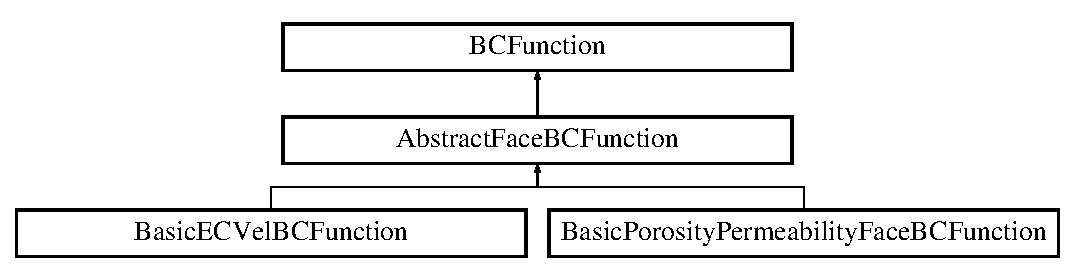
\includegraphics[height=3.000000cm]{class_abstract_face_b_c_function}
\end{center}
\end{figure}
\subsection*{Public Member Functions}
\begin{DoxyCompactItemize}
\item 
\hypertarget{class_abstract_face_b_c_function_afab41831f92499fc4d586c15c04a65e7}{\hyperlink{class_abstract_face_b_c_function_afab41831f92499fc4d586c15c04a65e7}{Abstract\-Face\-B\-C\-Function} ()}\label{class_abstract_face_b_c_function_afab41831f92499fc4d586c15c04a65e7}

\begin{DoxyCompactList}\small\item\em Default constructor. \end{DoxyCompactList}\item 
\hypertarget{class_abstract_face_b_c_function_a3a4587e8021aa687ad3903f99e415e1f}{\hyperlink{class_abstract_face_b_c_function_a3a4587e8021aa687ad3903f99e415e1f}{Abstract\-Face\-B\-C\-Function} (bool a\-\_\-is\-Homogeneous, int a\-\_\-comp, \hyperlink{class_mushy_layer_params}{Mushy\-Layer\-Params} a\-\_\-params)}\label{class_abstract_face_b_c_function_a3a4587e8021aa687ad3903f99e415e1f}

\begin{DoxyCompactList}\small\item\em Full constructor. \end{DoxyCompactList}\item 
\hypertarget{class_abstract_face_b_c_function_a7a864bc2f35778cd44d812c5c86db04b}{virtual void \hyperlink{class_abstract_face_b_c_function_a7a864bc2f35778cd44d812c5c86db04b}{operator()} (F\-Array\-Box \&a\-\_\-state, const Box \&a\-\_\-valid, const Problem\-Domain \&a\-\_\-domain, Real a\-\_\-dx, bool a\-\_\-homogeneous)=0}\label{class_abstract_face_b_c_function_a7a864bc2f35778cd44d812c5c86db04b}

\begin{DoxyCompactList}\small\item\em Apply B\-C. \end{DoxyCompactList}\item 
void \hyperlink{class_abstract_face_b_c_function_a176156d1142b51236652bbde0dee520a}{Diri\-Edge\-B\-C} (F\-Array\-Box \&a\-\_\-state, const Box \&a\-\_\-valid, Real a\-\_\-dx, bool a\-\_\-homogeneous, B\-C\-Value\-Holder a\-\_\-value, int a\-\_\-idir, Side\-::\-Lo\-Hi\-Side a\-\_\-side)
\item 
\hypertarget{class_abstract_face_b_c_function_a8a2f9d7139561aebae6dfd424d824fdb}{void \hyperlink{class_abstract_face_b_c_function_a8a2f9d7139561aebae6dfd424d824fdb}{Diri\-Edge\-Variable\-B\-C} (F\-Array\-Box \&a\-\_\-state, const Box \&a\-\_\-valid, Real a\-\_\-dx, bool a\-\_\-homogeneous, B\-C\-Value\-Holder a\-\_\-value, int a\-\_\-idir, Side\-::\-Lo\-Hi\-Side a\-\_\-side)}\label{class_abstract_face_b_c_function_a8a2f9d7139561aebae6dfd424d824fdb}

\begin{DoxyCompactList}\small\item\em Apply dirichlet B\-Cs (edge centred), allow different value at different locations. \end{DoxyCompactList}\item 
\hypertarget{class_abstract_face_b_c_function_a02f477a3ea7e1f91fa88815dadb1d9e9}{virtual void \hyperlink{class_abstract_face_b_c_function_a02f477a3ea7e1f91fa88815dadb1d9e9}{Neum\-Edge\-B\-C} (F\-Array\-Box \&a\-\_\-state, const Box \&a\-\_\-valid, Real a\-\_\-dx, bool a\-\_\-homogeneous, const B\-C\-Value\-Holder \&a\-\_\-value\-A, int a\-\_\-dir, Side\-::\-Lo\-Hi\-Side a\-\_\-side, Interval a\-\_\-interval)}\label{class_abstract_face_b_c_function_a02f477a3ea7e1f91fa88815dadb1d9e9}

\begin{DoxyCompactList}\small\item\em Apply neumann B\-Cs (edge centred) \end{DoxyCompactList}\end{DoxyCompactItemize}
\subsection*{Public Attributes}
\begin{DoxyCompactItemize}
\item 
\hypertarget{class_abstract_face_b_c_function_a68fdad0aa96f41e116e78f7488c9f747}{bool \hyperlink{class_abstract_face_b_c_function_a68fdad0aa96f41e116e78f7488c9f747}{m\-\_\-is\-Homogeneous}}\label{class_abstract_face_b_c_function_a68fdad0aa96f41e116e78f7488c9f747}

\begin{DoxyCompactList}\small\item\em Always enforce homogeneous form of B\-Cs? \end{DoxyCompactList}\item 
\hypertarget{class_abstract_face_b_c_function_ac626713cfdda3f62b9cece48abe03f2e}{int \hyperlink{class_abstract_face_b_c_function_ac626713cfdda3f62b9cece48abe03f2e}{m\-\_\-comp}}\label{class_abstract_face_b_c_function_ac626713cfdda3f62b9cece48abe03f2e}

\begin{DoxyCompactList}\small\item\em Component of velocity to apply B\-Cs to. \end{DoxyCompactList}\item 
\hypertarget{class_abstract_face_b_c_function_afe26ef4a7478bd64803699643d3dc11f}{\hyperlink{class_mushy_layer_params}{Mushy\-Layer\-Params} \hyperlink{class_abstract_face_b_c_function_afe26ef4a7478bd64803699643d3dc11f}{m\-\_\-params}}\label{class_abstract_face_b_c_function_afe26ef4a7478bd64803699643d3dc11f}

\begin{DoxyCompactList}\small\item\em Physical parameters for the problem. \end{DoxyCompactList}\end{DoxyCompactItemize}


\subsection{Detailed Description}
Note -\/ sets the same value along an entire boundary. 

\subsection{Member Function Documentation}
\hypertarget{class_abstract_face_b_c_function_a176156d1142b51236652bbde0dee520a}{\index{Abstract\-Face\-B\-C\-Function@{Abstract\-Face\-B\-C\-Function}!Diri\-Edge\-B\-C@{Diri\-Edge\-B\-C}}
\index{Diri\-Edge\-B\-C@{Diri\-Edge\-B\-C}!AbstractFaceBCFunction@{Abstract\-Face\-B\-C\-Function}}
\subsubsection[{Diri\-Edge\-B\-C}]{\setlength{\rightskip}{0pt plus 5cm}void Abstract\-Face\-B\-C\-Function\-::\-Diri\-Edge\-B\-C (
\begin{DoxyParamCaption}
\item[{F\-Array\-Box \&}]{a\-\_\-state, }
\item[{const Box \&}]{a\-\_\-valid, }
\item[{Real}]{a\-\_\-dx, }
\item[{bool}]{a\-\_\-homogeneous, }
\item[{B\-C\-Value\-Holder}]{a\-\_\-value, }
\item[{int}]{a\-\_\-idir, }
\item[{Side\-::\-Lo\-Hi\-Side}]{a\-\_\-side}
\end{DoxyParamCaption}
)\hspace{0.3cm}{\ttfamily [inline]}}}\label{class_abstract_face_b_c_function_a176156d1142b51236652bbde0dee520a}
Apply dirichlet B\-Cs (edge centred) apply the same B\-C value at all points 

The documentation for this class was generated from the following file\-:\begin{DoxyCompactItemize}
\item 
/home/parkinsonjl/mushy-\/layer/\-B\-Cutil/Phys\-B\-C\-Util.\-cpp\end{DoxyCompactItemize}

\hypertarget{class_abstract_scalar_b_c_function}{\section{Abstract\-Scalar\-B\-C\-Function Class Reference}
\label{class_abstract_scalar_b_c_function}\index{Abstract\-Scalar\-B\-C\-Function@{Abstract\-Scalar\-B\-C\-Function}}
}


Abstract scalar B\-C object.  


Inheritance diagram for Abstract\-Scalar\-B\-C\-Function\-:\begin{figure}[H]
\begin{center}
\leavevmode
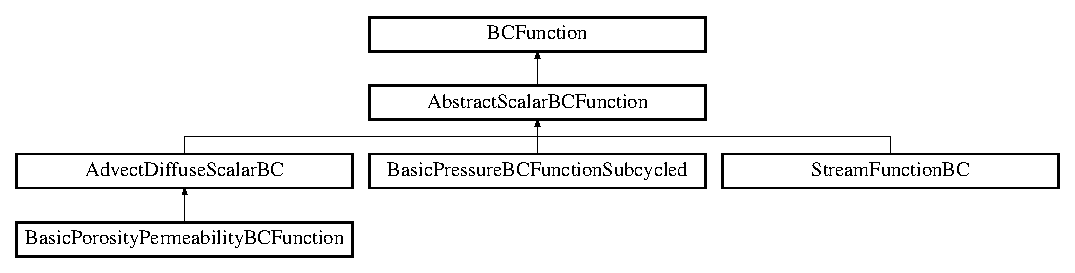
\includegraphics[height=3.218391cm]{class_abstract_scalar_b_c_function}
\end{center}
\end{figure}
\subsection*{Public Member Functions}
\begin{DoxyCompactItemize}
\item 
\hypertarget{class_abstract_scalar_b_c_function_ab17ecb34f1501f360d72fb3c2eb6d8a6}{\hyperlink{class_abstract_scalar_b_c_function_ab17ecb34f1501f360d72fb3c2eb6d8a6}{Abstract\-Scalar\-B\-C\-Function} ()}\label{class_abstract_scalar_b_c_function_ab17ecb34f1501f360d72fb3c2eb6d8a6}

\begin{DoxyCompactList}\small\item\em Default constructor. \end{DoxyCompactList}\item 
\hypertarget{class_abstract_scalar_b_c_function_ac391d3f5c821d7a7779b46388e89c221}{\hyperlink{class_abstract_scalar_b_c_function_ac391d3f5c821d7a7779b46388e89c221}{Abstract\-Scalar\-B\-C\-Function} (bool a\-\_\-is\-Defined, \hyperlink{class_mushy_layer_params}{Mushy\-Layer\-Params} a\-\_\-params, bool a\-\_\-homogeneous, Level\-Data$<$ Flux\-Box $>$ $\ast$a\-\_\-adv\-Vel, Real a\-\_\-dx, Interval a\-\_\-interval=Interval(0, 0))}\label{class_abstract_scalar_b_c_function_ac391d3f5c821d7a7779b46388e89c221}

\begin{DoxyCompactList}\small\item\em Full constructor. \end{DoxyCompactList}\item 
\hypertarget{class_abstract_scalar_b_c_function_a75298a4ff4835ee01361711eb73ea3ae}{virtual void \hyperlink{class_abstract_scalar_b_c_function_a75298a4ff4835ee01361711eb73ea3ae}{operator()} (F\-Array\-Box \&a\-\_\-state, const Box \&a\-\_\-valid, const Problem\-Domain \&a\-\_\-domain, Real a\-\_\-dx, bool a\-\_\-homogeneous)=0}\label{class_abstract_scalar_b_c_function_a75298a4ff4835ee01361711eb73ea3ae}

\begin{DoxyCompactList}\small\item\em Apply B\-C. \end{DoxyCompactList}\end{DoxyCompactItemize}
\subsection*{Public Attributes}
\begin{DoxyCompactItemize}
\item 
\hypertarget{class_abstract_scalar_b_c_function_ad13bee09bd7086a370e6f189d5641a29}{bool \hyperlink{class_abstract_scalar_b_c_function_ad13bee09bd7086a370e6f189d5641a29}{m\-\_\-is\-Defined}}\label{class_abstract_scalar_b_c_function_ad13bee09bd7086a370e6f189d5641a29}

\begin{DoxyCompactList}\small\item\em Is object defined? \end{DoxyCompactList}\item 
\hypertarget{class_abstract_scalar_b_c_function_a842c21b2fc8524d9f9c0b35ecb89e79b}{\hyperlink{class_mushy_layer_params}{Mushy\-Layer\-Params} \hyperlink{class_abstract_scalar_b_c_function_a842c21b2fc8524d9f9c0b35ecb89e79b}{m\-\_\-params}}\label{class_abstract_scalar_b_c_function_a842c21b2fc8524d9f9c0b35ecb89e79b}

\begin{DoxyCompactList}\small\item\em Physical parameters for the problem. \end{DoxyCompactList}\item 
\hypertarget{class_abstract_scalar_b_c_function_af24438d991ddc85df1f20f24a4a27ce8}{bool \hyperlink{class_abstract_scalar_b_c_function_af24438d991ddc85df1f20f24a4a27ce8}{m\-\_\-homogeneous}}\label{class_abstract_scalar_b_c_function_af24438d991ddc85df1f20f24a4a27ce8}

\begin{DoxyCompactList}\small\item\em Always enforce homogeneous B\-Cs? \end{DoxyCompactList}\item 
\hypertarget{class_abstract_scalar_b_c_function_a0c30e160f68816f2f87393397d76c4c6}{Level\-Data$<$ Flux\-Box $>$ $\ast$ \hyperlink{class_abstract_scalar_b_c_function_a0c30e160f68816f2f87393397d76c4c6}{m\-\_\-adv\-Vel}}\label{class_abstract_scalar_b_c_function_a0c30e160f68816f2f87393397d76c4c6}

\begin{DoxyCompactList}\small\item\em Advection velocity -\/ for inflow/outflow B\-Cs. \end{DoxyCompactList}\item 
\hypertarget{class_abstract_scalar_b_c_function_a32f08977d322c7c498a7567ed309d096}{Real \hyperlink{class_abstract_scalar_b_c_function_a32f08977d322c7c498a7567ed309d096}{m\-\_\-dx}}\label{class_abstract_scalar_b_c_function_a32f08977d322c7c498a7567ed309d096}

\begin{DoxyCompactList}\small\item\em Grid spacing for m\-\_\-adv\-Vel. \end{DoxyCompactList}\item 
\hypertarget{class_abstract_scalar_b_c_function_aeac3053b146f1138f2336e7d6562bf97}{Interval \hyperlink{class_abstract_scalar_b_c_function_aeac3053b146f1138f2336e7d6562bf97}{m\-\_\-interval}}\label{class_abstract_scalar_b_c_function_aeac3053b146f1138f2336e7d6562bf97}

\begin{DoxyCompactList}\small\item\em Interval to fill. \end{DoxyCompactList}\end{DoxyCompactItemize}


\subsection{Detailed Description}
Abstract scalar B\-C object. 

The documentation for this class was generated from the following file\-:\begin{DoxyCompactItemize}
\item 
/home/parkinsonjl/mushy-\/layer/\-B\-Cutil/Phys\-B\-C\-Util.\-cpp\end{DoxyCompactItemize}

\hypertarget{class_advect_diffuse_scalar_b_c}{\section{Advect\-Diffuse\-Scalar\-B\-C Class Reference}
\label{class_advect_diffuse_scalar_b_c}\index{Advect\-Diffuse\-Scalar\-B\-C@{Advect\-Diffuse\-Scalar\-B\-C}}
}


Scalar B\-C function which holds values at the top, bottom, and in the plume.  


Inheritance diagram for Advect\-Diffuse\-Scalar\-B\-C\-:\begin{figure}[H]
\begin{center}
\leavevmode
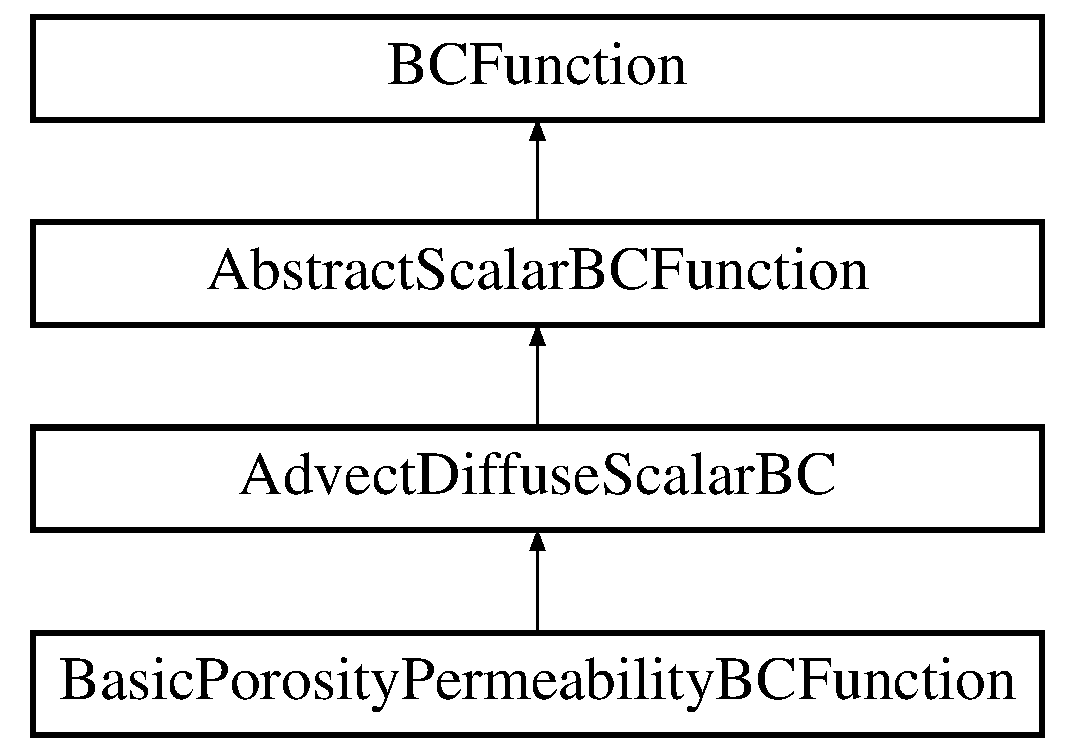
\includegraphics[height=4.000000cm]{class_advect_diffuse_scalar_b_c}
\end{center}
\end{figure}
\subsection*{Public Member Functions}
\begin{DoxyCompactItemize}
\item 
\hypertarget{class_advect_diffuse_scalar_b_c_a2227cd96500613d5eb7918cc6fa3a645}{{\bfseries Advect\-Diffuse\-Scalar\-B\-C} (bool a\-\_\-is\-Defined, \hyperlink{class_mushy_layer_params}{Mushy\-Layer\-Params} a\-\_\-params, bool a\-\_\-homogeneous, Level\-Data$<$ Flux\-Box $>$ $\ast$a\-\_\-adv\-Vel, Real a\-\_\-dx, Vector$<$ Real $>$ a\-\_\-plume\-Vals, Interval a\-\_\-interval, Vector$<$ Vector$<$ int $>$ $>$ \&a\-\_\-custom\-Lo\-B\-C, Vector$<$ Vector$<$ int $>$ $>$ \&a\-\_\-custom\-Hi\-B\-C, Vector$<$ Vector$<$ Real $>$ $>$ \&a\-\_\-custom\-Lo\-B\-C\-Val, Vector$<$ Vector$<$ Real $>$ $>$ \&a\-\_\-custom\-Hi\-B\-C\-Val)}\label{class_advect_diffuse_scalar_b_c_a2227cd96500613d5eb7918cc6fa3a645}

\item 
\hypertarget{class_advect_diffuse_scalar_b_c_ab55b1f2a27a3ff1ecda0d56acdbf0d77}{virtual void \hyperlink{class_advect_diffuse_scalar_b_c_ab55b1f2a27a3ff1ecda0d56acdbf0d77}{operator()} (F\-Array\-Box \&a\-\_\-state, const Box \&a\-\_\-valid, const Problem\-Domain \&a\-\_\-domain, Real a\-\_\-dx, bool a\-\_\-homogeneous)}\label{class_advect_diffuse_scalar_b_c_ab55b1f2a27a3ff1ecda0d56acdbf0d77}

\begin{DoxyCompactList}\small\item\em Apply B\-C. \end{DoxyCompactList}\end{DoxyCompactItemize}
\subsection*{Public Attributes}
\begin{DoxyCompactItemize}
\item 
\hypertarget{class_advect_diffuse_scalar_b_c_a24079c63607fa7aaada70d393c91038e}{Vector$<$ Real $>$ {\bfseries m\-\_\-plume\-Val}}\label{class_advect_diffuse_scalar_b_c_a24079c63607fa7aaada70d393c91038e}

\item 
\hypertarget{class_advect_diffuse_scalar_b_c_a88722dbb4d1fde30f3608db8104640c0}{Vector$<$ Vector$<$ int $>$ $>$ \hyperlink{class_advect_diffuse_scalar_b_c_a88722dbb4d1fde30f3608db8104640c0}{m\-\_\-custom\-Lo\-B\-C}}\label{class_advect_diffuse_scalar_b_c_a88722dbb4d1fde30f3608db8104640c0}

\begin{DoxyCompactList}\small\item\em Each element of the vector corresponds to a different interval. \end{DoxyCompactList}\item 
\hypertarget{class_advect_diffuse_scalar_b_c_a3143ed8cc319ce90e64e936c459f9b12}{Vector$<$ Vector$<$ int $>$ $>$ {\bfseries m\-\_\-custom\-Hi\-B\-C}}\label{class_advect_diffuse_scalar_b_c_a3143ed8cc319ce90e64e936c459f9b12}

\item 
\hypertarget{class_advect_diffuse_scalar_b_c_ab09adbfb8bbf7bd9ec9d51f2d0b1106a}{Vector$<$ Vector$<$ Real $>$ $>$ {\bfseries m\-\_\-custom\-Lo\-B\-C\-Val}}\label{class_advect_diffuse_scalar_b_c_ab09adbfb8bbf7bd9ec9d51f2d0b1106a}

\item 
\hypertarget{class_advect_diffuse_scalar_b_c_a5733082dd61f2021d755cfebda84481d}{Vector$<$ Vector$<$ Real $>$ $>$ {\bfseries m\-\_\-custom\-Hi\-B\-C\-Val}}\label{class_advect_diffuse_scalar_b_c_a5733082dd61f2021d755cfebda84481d}

\end{DoxyCompactItemize}


\subsection{Detailed Description}
Scalar B\-C function which holds values at the top, bottom, and in the plume. 

All these fields have the same type of conditions at each boundary, but just different values. 

The documentation for this class was generated from the following file\-:\begin{DoxyCompactItemize}
\item 
/home/parkinsonjl/mushy-\/layer/\-B\-Cutil/Phys\-B\-C\-Util.\-cpp\end{DoxyCompactItemize}

\hypertarget{class_advect_i_b_c}{\section{Advect\-I\-B\-C Class Reference}
\label{class_advect_i_b_c}\index{Advect\-I\-B\-C@{Advect\-I\-B\-C}}
}


I\-B\-C for simple advection.  




{\ttfamily \#include $<$Advect\-I\-B\-C.\-H$>$}

Inheritance diagram for Advect\-I\-B\-C\-:\begin{figure}[H]
\begin{center}
\leavevmode
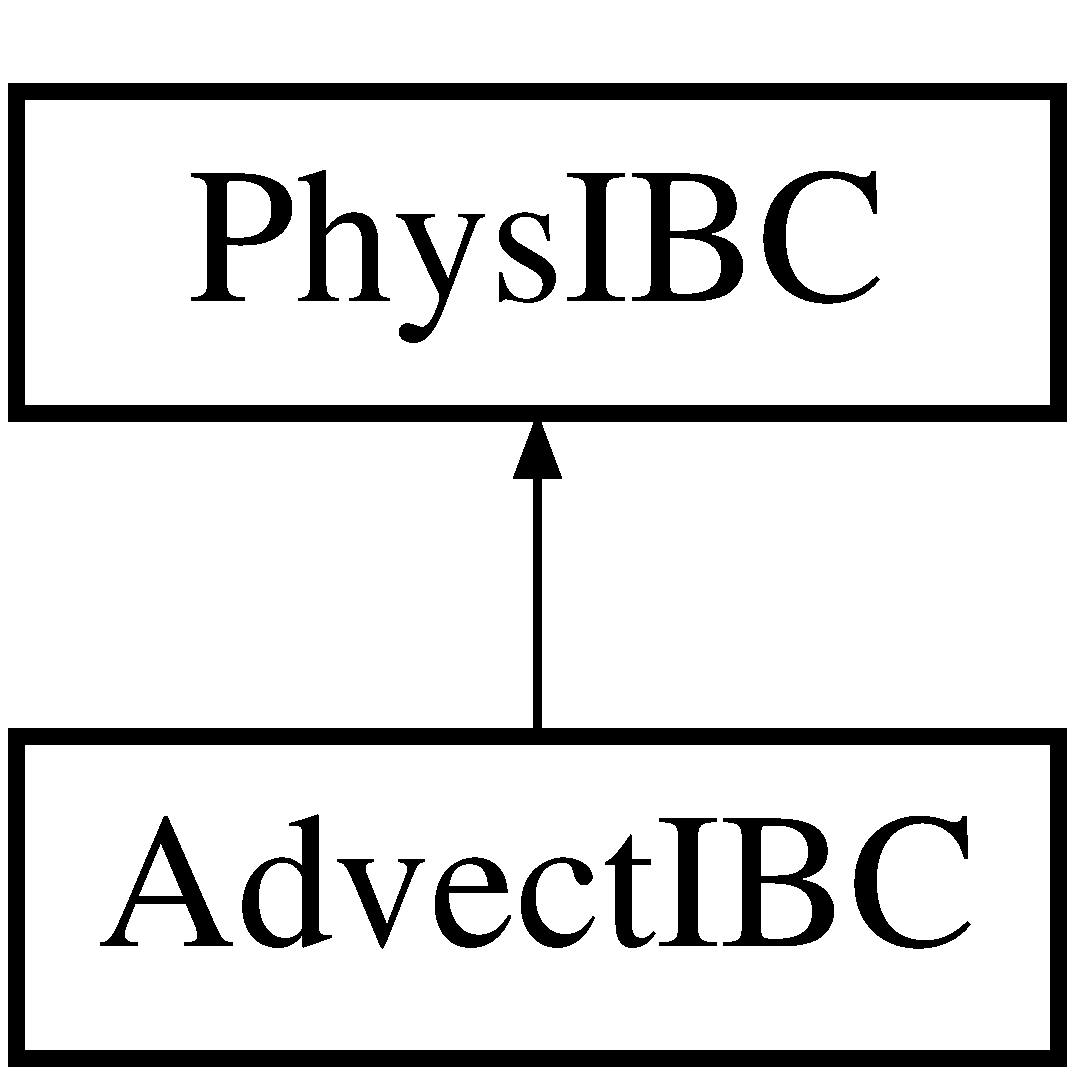
\includegraphics[height=2.000000cm]{class_advect_i_b_c}
\end{center}
\end{figure}
\subsection*{Public Types}
\begin{DoxyCompactItemize}
\item 
enum \hyperlink{class_advect_i_b_c_ad4d8474d7904dab87483522ebe711b8e}{bc\-Type} \{ \\*
{\bfseries m\-\_\-dirichlet}, 
{\bfseries m\-\_\-extrap}, 
{\bfseries m\-\_\-inflow\-Outflow}, 
{\bfseries m\-\_\-plume\-Inflow}, 
\\*
{\bfseries m\-\_\-neumann}, 
{\bfseries m\-\_\-num\-B\-C\-Types}
 \}
\begin{DoxyCompactList}\small\item\em Possible B\-C types. \end{DoxyCompactList}\end{DoxyCompactItemize}
\subsection*{Public Member Functions}
\begin{DoxyCompactItemize}
\item 
\hypertarget{class_advect_i_b_c_af2d3f4fff7f08be3e1e3f140034bc34c}{\hyperlink{class_advect_i_b_c_af2d3f4fff7f08be3e1e3f140034bc34c}{Advect\-I\-B\-C} ()}\label{class_advect_i_b_c_af2d3f4fff7f08be3e1e3f140034bc34c}

\begin{DoxyCompactList}\small\item\em Null constructor. \end{DoxyCompactList}\item 
\hypertarget{class_advect_i_b_c_a8897e6ad80cdff2121c4d4f6ce922ce1}{{\bfseries Advect\-I\-B\-C} (int a\-\_\-num\-Comp)}\label{class_advect_i_b_c_a8897e6ad80cdff2121c4d4f6ce922ce1}

\item 
\hypertarget{class_advect_i_b_c_a4d1d956949384ad8621ba145de87952e}{\hyperlink{class_advect_i_b_c_a4d1d956949384ad8621ba145de87952e}{$\sim$\-Advect\-I\-B\-C} ()}\label{class_advect_i_b_c_a4d1d956949384ad8621ba145de87952e}

\begin{DoxyCompactList}\small\item\em Destructor. \end{DoxyCompactList}\item 
Phys\-I\-B\-C $\ast$ \hyperlink{class_advect_i_b_c_a4d092d4a393e169a87f7df920d09a2b0}{new\-\_\-phys\-I\-B\-C} ()
\begin{DoxyCompactList}\small\item\em Factory method -\/ this object is its own factory. \end{DoxyCompactList}\item 
\hypertarget{class_advect_i_b_c_ae2edb5fa139b1655c3d7d87416da7023}{void \hyperlink{class_advect_i_b_c_ae2edb5fa139b1655c3d7d87416da7023}{set\-Default\-Values} (int a\-\_\-num\-Comp=1)}\label{class_advect_i_b_c_ae2edb5fa139b1655c3d7d87416da7023}

\begin{DoxyCompactList}\small\item\em set default boundary values \end{DoxyCompactList}\item 
\hypertarget{class_advect_i_b_c_af222561d9fba9498f4fc647a9e37547a}{void \hyperlink{class_advect_i_b_c_af222561d9fba9498f4fc647a9e37547a}{prim\-B\-C} (F\-Array\-Box \&a\-\_\-\-W\-Gdnv, const F\-Array\-Box \&a\-\_\-\-Wextrap, const F\-Array\-Box \&a\-\_\-\-W, const int \&a\-\_\-dir, const Side\-::\-Lo\-Hi\-Side \&a\-\_\-side, const Real \&a\-\_\-time)}\label{class_advect_i_b_c_af222561d9fba9498f4fc647a9e37547a}

\begin{DoxyCompactList}\small\item\em Set boundary fluxes. \end{DoxyCompactList}\item 
void \hyperlink{class_advect_i_b_c_a5410c1910c93274665fe324a5c6b3be9}{set\-Bdry\-Slopes} (F\-Array\-Box \&a\-\_\-d\-W, const F\-Array\-Box \&a\-\_\-\-W, const int \&a\-\_\-dir, const Real \&a\-\_\-time)
\begin{DoxyCompactList}\small\item\em Set boundary slopes. \end{DoxyCompactList}\item 
void \hyperlink{class_advect_i_b_c_abd44c883d18c238c99456b57d974f9dc}{initialize} (Level\-Data$<$ F\-Array\-Box $>$ \&a\-\_\-\-U)
\begin{DoxyCompactList}\small\item\em Set up initial conditions. \end{DoxyCompactList}\item 
\hypertarget{class_advect_i_b_c_ab09d9d22d56f103e39e08884fb4b6217}{void \hyperlink{class_advect_i_b_c_ab09d9d22d56f103e39e08884fb4b6217}{advection\-Vel} (const Real\-Vect \&a\-\_\-adv\-Vel)}\label{class_advect_i_b_c_ab09d9d22d56f103e39e08884fb4b6217}

\begin{DoxyCompactList}\small\item\em set velocity \end{DoxyCompactList}\item 
\hypertarget{class_advect_i_b_c_a249a4f558a5cfa9b51874cc6d51df02a}{const Real\-Vect \& \hyperlink{class_advect_i_b_c_a249a4f558a5cfa9b51874cc6d51df02a}{advection\-Vel} () const }\label{class_advect_i_b_c_a249a4f558a5cfa9b51874cc6d51df02a}

\begin{DoxyCompactList}\small\item\em advection velocity. No idea what this is here for. \end{DoxyCompactList}\item 
\hypertarget{class_advect_i_b_c_ab835398d8c5f12740518e69d47e8cad2}{void \hyperlink{class_advect_i_b_c_ab835398d8c5f12740518e69d47e8cad2}{prob\-Type} (const int a\-\_\-probtype)}\label{class_advect_i_b_c_ab835398d8c5f12740518e69d47e8cad2}

\begin{DoxyCompactList}\small\item\em set problem type \end{DoxyCompactList}\item 
\hypertarget{class_advect_i_b_c_a9d9cb1bf0ce09b8f4ce0429b850221a7}{void \hyperlink{class_advect_i_b_c_a9d9cb1bf0ce09b8f4ce0429b850221a7}{set\-Boundary\-Value} (Real a\-\_\-bc\-Val, int a\-\_\-bc\-Type, int a\-\_\-dir, Side\-::\-Lo\-Hi\-Side a\-\_\-hi\-Lo, int a\-\_\-comp=0)}\label{class_advect_i_b_c_a9d9cb1bf0ce09b8f4ce0429b850221a7}

\begin{DoxyCompactList}\small\item\em set boundary value (default is 0) \end{DoxyCompactList}\item 
\hypertarget{class_advect_i_b_c_aa03fa005397fe7ba2f40dfd0e4762f66}{void \hyperlink{class_advect_i_b_c_aa03fa005397fe7ba2f40dfd0e4762f66}{set\-Boundary\-Values} (Real\-Vect bc\-Vals, Int\-Vect \hyperlink{class_advect_i_b_c_ad4d8474d7904dab87483522ebe711b8e}{bc\-Type}, Side\-::\-Lo\-Hi\-Side a\-\_\-hi\-Lo, int a\-\_\-comp=0)}\label{class_advect_i_b_c_aa03fa005397fe7ba2f40dfd0e4762f66}

\begin{DoxyCompactList}\small\item\em Set boundary values (N dimensional version) \end{DoxyCompactList}\item 
\hypertarget{class_advect_i_b_c_a559e2f450c3ccbff23ba713d508117d5}{void \hyperlink{class_advect_i_b_c_a559e2f450c3ccbff23ba713d508117d5}{set\-Plume} (Vector$<$ Real $>$ a\-\_\-plume\-Vals, Vector$<$ Real $>$ plume\-Bounds)}\label{class_advect_i_b_c_a559e2f450c3ccbff23ba713d508117d5}

\begin{DoxyCompactList}\small\item\em Set plume details. \end{DoxyCompactList}\item 
\hypertarget{class_advect_i_b_c_abeb87fbdca5e7f2711161712734c3f9e}{void \hyperlink{class_advect_i_b_c_abeb87fbdca5e7f2711161712734c3f9e}{set\-B\-C\-Type} (int a\-\_\-bc\-Type, int a\-\_\-dir, Side\-::\-Lo\-Hi\-Side a\-\_\-hi\-Lo)}\label{class_advect_i_b_c_abeb87fbdca5e7f2711161712734c3f9e}

\begin{DoxyCompactList}\small\item\em Set the type of condition on each boundary. \end{DoxyCompactList}\item 
\hypertarget{class_advect_i_b_c_adabceffc28ca37c3be7a6fc3f674c69b}{Real \hyperlink{class_advect_i_b_c_adabceffc28ca37c3be7a6fc3f674c69b}{get\-Boundary\-Value} (int a\-\_\-dir, Side\-::\-Lo\-Hi\-Side a\-\_\-hi\-Lo, int a\-\_\-comp=0) const }\label{class_advect_i_b_c_adabceffc28ca37c3be7a6fc3f674c69b}

\begin{DoxyCompactList}\small\item\em access boundary value \end{DoxyCompactList}\item 
\hypertarget{class_advect_i_b_c_a28147c7f8464b4f5ce98813a277799ad}{void \hyperlink{class_advect_i_b_c_a28147c7f8464b4f5ce98813a277799ad}{set\-Adv\-Vel} (Level\-Data$<$ Flux\-Box $>$ $\ast$a\-\_\-adv\-Vel)}\label{class_advect_i_b_c_a28147c7f8464b4f5ce98813a277799ad}

\begin{DoxyCompactList}\small\item\em Set pointer to advection velocity. \end{DoxyCompactList}\item 
\hypertarget{class_advect_i_b_c_aae3c93645117a85f8ed4efbc758d9cc6}{void \hyperlink{class_advect_i_b_c_aae3c93645117a85f8ed4efbc758d9cc6}{set\-Adv\-Vel} (Flux\-Box $\ast$a\-\_\-adv\-Vel)}\label{class_advect_i_b_c_aae3c93645117a85f8ed4efbc758d9cc6}

\begin{DoxyCompactList}\small\item\em Set pointer to advection velocity for the box we're integrating over. \end{DoxyCompactList}\item 
\hypertarget{class_advect_i_b_c_a142042663359db469a777366ca287855}{void \hyperlink{class_advect_i_b_c_a142042663359db469a777366ca287855}{set\-Slope\-Value} (Real a\-\_\-slope\-Val, int a\-\_\-dir, Side\-::\-Lo\-Hi\-Side a\-\_\-hi\-Lo)}\label{class_advect_i_b_c_a142042663359db469a777366ca287855}

\begin{DoxyCompactList}\small\item\em set slope value (default is 0) \end{DoxyCompactList}\item 
\hypertarget{class_advect_i_b_c_a8feb7b809940db26555a59073cdb9de7}{Real \hyperlink{class_advect_i_b_c_a8feb7b809940db26555a59073cdb9de7}{get\-Slope\-Value} (int a\-\_\-dir, Side\-::\-Lo\-Hi\-Side a\-\_\-hi\-Lo) const }\label{class_advect_i_b_c_a8feb7b809940db26555a59073cdb9de7}

\begin{DoxyCompactList}\small\item\em access slope value \end{DoxyCompactList}\item 
\hypertarget{class_advect_i_b_c_a8109239cfc7cc3637da64045e4df1f30}{void \hyperlink{class_advect_i_b_c_a8109239cfc7cc3637da64045e4df1f30}{art\-Visc\-B\-C} (F\-Array\-Box \&a\-\_\-\-F, const F\-Array\-Box \&a\-\_\-\-U, const F\-Array\-Box \&a\-\_\-div\-Vel, const int \&a\-\_\-dir, const Real \&a\-\_\-time)}\label{class_advect_i_b_c_a8109239cfc7cc3637da64045e4df1f30}

\begin{DoxyCompactList}\small\item\em Apply artifical viscosity B\-Cs. \end{DoxyCompactList}\item 
\hypertarget{class_advect_i_b_c_ae61302d20370083b3d249c994aa368da}{int \hyperlink{class_advect_i_b_c_ae61302d20370083b3d249c994aa368da}{prob\-Type} () const }\label{class_advect_i_b_c_ae61302d20370083b3d249c994aa368da}

\begin{DoxyCompactList}\small\item\em accessor \end{DoxyCompactList}\end{DoxyCompactItemize}
\subsection*{Protected Attributes}
\begin{DoxyCompactItemize}
\item 
\hypertarget{class_advect_i_b_c_a7d844d0407883309028ab564f3b20261}{Real\-Vect \hyperlink{class_advect_i_b_c_a7d844d0407883309028ab564f3b20261}{m\-\_\-velocity}}\label{class_advect_i_b_c_a7d844d0407883309028ab564f3b20261}

\begin{DoxyCompactList}\small\item\em Don't know what this is for. \end{DoxyCompactList}\item 
\hypertarget{class_advect_i_b_c_a5737cd993143b522c10599caa94e849f}{Real \hyperlink{class_advect_i_b_c_a5737cd993143b522c10599caa94e849f}{m\-\_\-bc\-Val\-Plume}}\label{class_advect_i_b_c_a5737cd993143b522c10599caa94e849f}

\begin{DoxyCompactList}\small\item\em boundary value at the plume \end{DoxyCompactList}\item 
\hypertarget{class_advect_i_b_c_aeb567fe955fff5c26c250a77b1bd2762}{Real {\bfseries m\-\_\-inflow\-Val}}\label{class_advect_i_b_c_aeb567fe955fff5c26c250a77b1bd2762}

\item 
\hypertarget{class_advect_i_b_c_a4149bd47a240acfc4de71ff74e10df1d}{Vector$<$ Real $>$ {\bfseries m\-\_\-plume\-Bounds}}\label{class_advect_i_b_c_a4149bd47a240acfc4de71ff74e10df1d}

\item 
\hypertarget{class_advect_i_b_c_a2fd99ddeaa84fbadf49657de8491998f}{Level\-Data$<$ Flux\-Box $>$ $\ast$ \hyperlink{class_advect_i_b_c_a2fd99ddeaa84fbadf49657de8491998f}{m\-\_\-adv\-Vel}}\label{class_advect_i_b_c_a2fd99ddeaa84fbadf49657de8491998f}

\begin{DoxyCompactList}\small\item\em advection velocity field for the whole level \end{DoxyCompactList}\item 
\hypertarget{class_advect_i_b_c_a34ee29705f4f1205a75f0c725a135a1a}{Flux\-Box $\ast$ \hyperlink{class_advect_i_b_c_a34ee29705f4f1205a75f0c725a135a1a}{m\-\_\-adv\-Vel\-Box}}\label{class_advect_i_b_c_a34ee29705f4f1205a75f0c725a135a1a}

\begin{DoxyCompactList}\small\item\em advection velocity for the specific box we're integrating over \end{DoxyCompactList}\item 
\hypertarget{class_advect_i_b_c_a8d828241433e76c184521c9ae489f078}{Vector$<$ Real $>$ \hyperlink{class_advect_i_b_c_a8d828241433e76c184521c9ae489f078}{m\-\_\-bc\-Val} \mbox{[}Space\-Dim\mbox{]}\mbox{[}2\mbox{]}}\label{class_advect_i_b_c_a8d828241433e76c184521c9ae489f078}

\begin{DoxyCompactList}\small\item\em Boundary value. \end{DoxyCompactList}\item 
\hypertarget{class_advect_i_b_c_a4f7653572eab6fea3ad343517b9f87c6}{Real \hyperlink{class_advect_i_b_c_a4f7653572eab6fea3ad343517b9f87c6}{m\-\_\-slope\-Val} \mbox{[}Space\-Dim\mbox{]}\mbox{[}2\mbox{]}}\label{class_advect_i_b_c_a4f7653572eab6fea3ad343517b9f87c6}

\begin{DoxyCompactList}\small\item\em Boundary slope value. \end{DoxyCompactList}\item 
\hypertarget{class_advect_i_b_c_a690ab64b62ebfc1757ec94dc93706516}{Vector$<$ Real $>$ {\bfseries m\-\_\-plume\-Vals}}\label{class_advect_i_b_c_a690ab64b62ebfc1757ec94dc93706516}

\item 
\hypertarget{class_advect_i_b_c_aa2a891f499c8d490a7ac7531a33a5d85}{Vector$<$ int $>$ \hyperlink{class_advect_i_b_c_aa2a891f499c8d490a7ac7531a33a5d85}{m\-\_\-bc\-Type} \mbox{[}Space\-Dim\mbox{]}\mbox{[}2\mbox{]}}\label{class_advect_i_b_c_aa2a891f499c8d490a7ac7531a33a5d85}

\begin{DoxyCompactList}\small\item\em Boundary condition type. \end{DoxyCompactList}\item 
\hypertarget{class_advect_i_b_c_a3efbc8664456083ae4d71de9a7b17312}{bool \hyperlink{class_advect_i_b_c_a3efbc8664456083ae4d71de9a7b17312}{m\-\_\-is\-B\-Cval\-Set}}\label{class_advect_i_b_c_a3efbc8664456083ae4d71de9a7b17312}

\begin{DoxyCompactList}\small\item\em Whether or not B\-Cs have been set. \end{DoxyCompactList}\item 
\hypertarget{class_advect_i_b_c_afd9c2bb5aa7834ea549538f060857ba9}{bool \hyperlink{class_advect_i_b_c_afd9c2bb5aa7834ea549538f060857ba9}{m\-\_\-is\-Slope\-Val\-Set}}\label{class_advect_i_b_c_afd9c2bb5aa7834ea549538f060857ba9}

\begin{DoxyCompactList}\small\item\em Whether or not boundary slopes have been set. \end{DoxyCompactList}\item 
\hypertarget{class_advect_i_b_c_acccc5b94b75465b61128a7b8075516ae}{bool \hyperlink{class_advect_i_b_c_acccc5b94b75465b61128a7b8075516ae}{m\-\_\-is\-B\-Ctype\-Set}}\label{class_advect_i_b_c_acccc5b94b75465b61128a7b8075516ae}

\begin{DoxyCompactList}\small\item\em Whether or not B\-C types have been set. \end{DoxyCompactList}\item 
\hypertarget{class_advect_i_b_c_afcdc8bf740b7e44790927adce875cf59}{int \hyperlink{class_advect_i_b_c_afcdc8bf740b7e44790927adce875cf59}{m\-\_\-num\-Comps}}\label{class_advect_i_b_c_afcdc8bf740b7e44790927adce875cf59}

\begin{DoxyCompactList}\small\item\em number of components \end{DoxyCompactList}\end{DoxyCompactItemize}


\subsection{Detailed Description}
I\-B\-C for simple advection. 

Parameters\-: 

\subsection{Member Function Documentation}
\hypertarget{class_advect_i_b_c_abd44c883d18c238c99456b57d974f9dc}{\index{Advect\-I\-B\-C@{Advect\-I\-B\-C}!initialize@{initialize}}
\index{initialize@{initialize}!AdvectIBC@{Advect\-I\-B\-C}}
\subsubsection[{initialize}]{\setlength{\rightskip}{0pt plus 5cm}void Advect\-I\-B\-C\-::initialize (
\begin{DoxyParamCaption}
\item[{Level\-Data$<$ F\-Array\-Box $>$ \&}]{a\-\_\-\-U}
\end{DoxyParamCaption}
)}}\label{class_advect_i_b_c_abd44c883d18c238c99456b57d974f9dc}


Set up initial conditions. 

shouldn't be in this function \hypertarget{class_advect_i_b_c_a4d092d4a393e169a87f7df920d09a2b0}{\index{Advect\-I\-B\-C@{Advect\-I\-B\-C}!new\-\_\-phys\-I\-B\-C@{new\-\_\-phys\-I\-B\-C}}
\index{new\-\_\-phys\-I\-B\-C@{new\-\_\-phys\-I\-B\-C}!AdvectIBC@{Advect\-I\-B\-C}}
\subsubsection[{new\-\_\-phys\-I\-B\-C}]{\setlength{\rightskip}{0pt plus 5cm}Phys\-I\-B\-C $\ast$ Advect\-I\-B\-C\-::new\-\_\-phys\-I\-B\-C (
\begin{DoxyParamCaption}
{}
\end{DoxyParamCaption}
)}}\label{class_advect_i_b_c_a4d092d4a393e169a87f7df920d09a2b0}


Factory method -\/ this object is its own factory. 

Return a pointer to a new Phys\-I\-B\-C object with m\-\_\-is\-Defined = false (i.\-e., its define() must be called before it is used) and m\-\_\-is\-Fortran\-Common\-Set set to value of m\-\_\-is\-Fortran\-Commonset in the current (factory) object. \hypertarget{class_advect_i_b_c_a5410c1910c93274665fe324a5c6b3be9}{\index{Advect\-I\-B\-C@{Advect\-I\-B\-C}!set\-Bdry\-Slopes@{set\-Bdry\-Slopes}}
\index{set\-Bdry\-Slopes@{set\-Bdry\-Slopes}!AdvectIBC@{Advect\-I\-B\-C}}
\subsubsection[{set\-Bdry\-Slopes}]{\setlength{\rightskip}{0pt plus 5cm}void Advect\-I\-B\-C\-::set\-Bdry\-Slopes (
\begin{DoxyParamCaption}
\item[{F\-Array\-Box \&}]{a\-\_\-d\-W, }
\item[{const F\-Array\-Box \&}]{a\-\_\-\-W, }
\item[{const int \&}]{a\-\_\-dir, }
\item[{const Real \&}]{a\-\_\-time}
\end{DoxyParamCaption}
)}}\label{class_advect_i_b_c_a5410c1910c93274665fe324a5c6b3be9}


Set boundary slopes. 

The boundary slopes in a\-\_\-d\-W are already set to one sided difference approximations. If this function doesn't change them they will be used for the slopes at the boundaries. 

The documentation for this class was generated from the following files\-:\begin{DoxyCompactItemize}
\item 
/home/parkinsonjl/mushy-\/layer/\-B\-Cutil/Advect\-I\-B\-C.\-H\item 
/home/parkinsonjl/mushy-\/layer/\-B\-Cutil/Advect\-I\-B\-C.\-cpp\end{DoxyCompactItemize}

\hypertarget{class_advection_physics}{\section{Advection\-Physics Class Reference}
\label{class_advection_physics}\index{Advection\-Physics@{Advection\-Physics}}
}


An Godunov\-Physics-\/derived class for simple advection-\/diffusion problems.  




{\ttfamily \#include $<$Advection\-Physics.\-H$>$}

Inheritance diagram for Advection\-Physics\-:\begin{figure}[H]
\begin{center}
\leavevmode
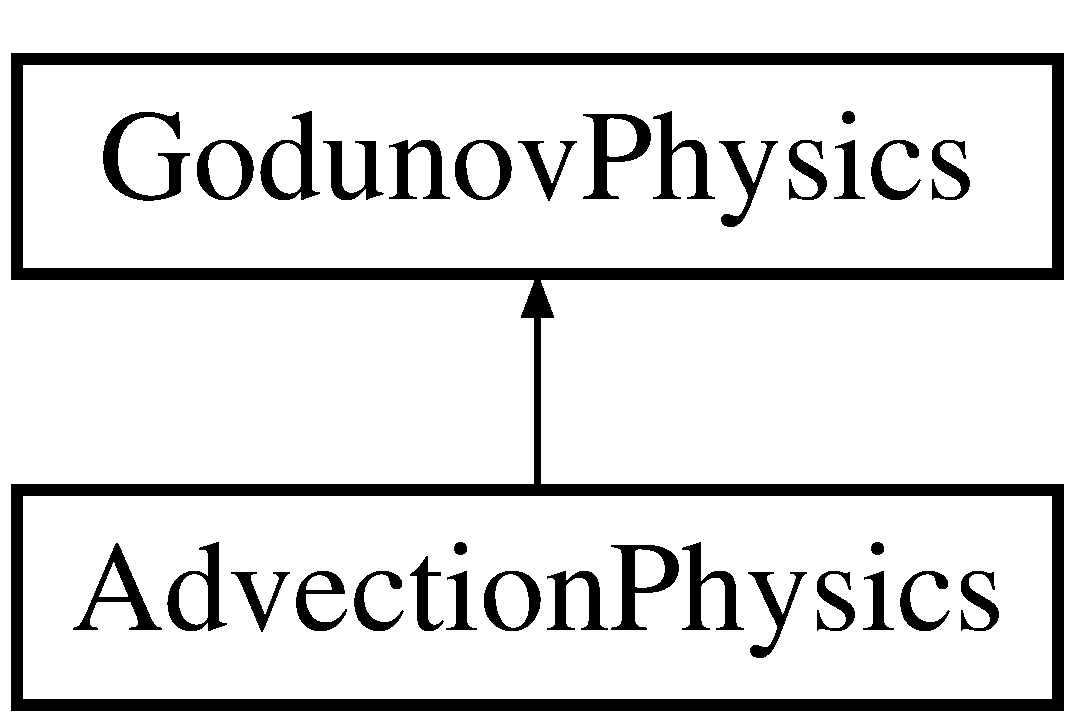
\includegraphics[height=2.000000cm]{class_advection_physics}
\end{center}
\end{figure}
\subsection*{Public Member Functions}
\begin{DoxyCompactItemize}
\item 
\hypertarget{class_advection_physics_ac392278448ed29a685f9562f709a5b4b}{\hyperlink{class_advection_physics_ac392278448ed29a685f9562f709a5b4b}{Advection\-Physics} ()}\label{class_advection_physics_ac392278448ed29a685f9562f709a5b4b}

\begin{DoxyCompactList}\small\item\em Constructor. \end{DoxyCompactList}\item 
\hypertarget{class_advection_physics_a90f848be0b676fed24227e782aec2eb6}{\hyperlink{class_advection_physics_a90f848be0b676fed24227e782aec2eb6}{$\sim$\-Advection\-Physics} ()}\label{class_advection_physics_a90f848be0b676fed24227e782aec2eb6}

\begin{DoxyCompactList}\small\item\em Destructor. \end{DoxyCompactList}\item 
\hypertarget{class_advection_physics_ad50a0a57026615c8d7fd14d8e523f463}{virtual void \hyperlink{class_advection_physics_ad50a0a57026615c8d7fd14d8e523f463}{set\-N\-Comp} (int a\-\_\-n\-Comp)}\label{class_advection_physics_ad50a0a57026615c8d7fd14d8e523f463}

\begin{DoxyCompactList}\small\item\em Set the number of components. \end{DoxyCompactList}\item 
\hypertarget{class_advection_physics_a4305b9cac37f64a32c3db11a28068944}{virtual Real \hyperlink{class_advection_physics_a4305b9cac37f64a32c3db11a28068944}{get\-Max\-Wave\-Speed} (const F\-Array\-Box \&a\-\_\-\-U, const Box \&a\-\_\-box)}\label{class_advection_physics_a4305b9cac37f64a32c3db11a28068944}

\begin{DoxyCompactList}\small\item\em Compute the maximum wave speed. \end{DoxyCompactList}\item 
virtual Godunov\-Physics $\ast$ \hyperlink{class_advection_physics_abbf17dd7a6726453af2e94d9ce1b5686}{new\-\_\-godunov\-Physics} () const 
\begin{DoxyCompactList}\small\item\em Factory method -\/ this object is its own factory. \end{DoxyCompactList}\item 
virtual int \hyperlink{class_advection_physics_ab139a3b1201a76e97e918381c5b3ff98}{num\-Conserved} ()
\begin{DoxyCompactList}\small\item\em Number of conserved variables. \end{DoxyCompactList}\item 
virtual Vector$<$ string $>$ \hyperlink{class_advection_physics_a992f0d9ca9515de44b82981c14a2fb31}{state\-Names} ()
\begin{DoxyCompactList}\small\item\em Names of the conserved variables. \end{DoxyCompactList}\item 
virtual int \hyperlink{class_advection_physics_ab59b268a446dbe2912e000c11870ab2f}{num\-Fluxes} ()
\begin{DoxyCompactList}\small\item\em Number of flux variables. \end{DoxyCompactList}\item 
virtual void \hyperlink{class_advection_physics_a469e6262703804372173e378c37b735f}{get\-Flux} (F\-Array\-Box \&a\-\_\-flux, const F\-Array\-Box \&a\-\_\-\-W\-Half, const int \&a\-\_\-dir, const Box \&a\-\_\-box)
\begin{DoxyCompactList}\small\item\em compute fluxes from primitive values on a face ( adv\-Vel$\ast$w\-Half) \end{DoxyCompactList}\item 
virtual bool \hyperlink{class_advection_physics_ac35ee4f5f59fd7c9af605b47af635f8e}{is\-Defined} () const 
\begin{DoxyCompactList}\small\item\em Is the object completely defined. \end{DoxyCompactList}\item 
virtual int \hyperlink{class_advection_physics_ad00c2d52ec684668ff5cd1da9eed42bf}{num\-Primitives} ()
\begin{DoxyCompactList}\small\item\em Number of primitve variables. \end{DoxyCompactList}\item 
virtual void \hyperlink{class_advection_physics_a63895f9dd1173d14684c0681653c8d36}{char\-Analysis} (F\-Array\-Box \&a\-\_\-d\-W, const F\-Array\-Box \&a\-\_\-\-W, const int \&a\-\_\-dir, const Box \&a\-\_\-box)
\begin{DoxyCompactList}\small\item\em Transform a\-\_\-d\-W from primitive to characteristic variables. \end{DoxyCompactList}\item 
virtual void \hyperlink{class_advection_physics_a8b1269b718057fe2a5d0bc8bdd183d0b}{char\-Synthesis} (F\-Array\-Box \&a\-\_\-d\-W, const F\-Array\-Box \&a\-\_\-\-W, const int \&a\-\_\-dir, const Box \&a\-\_\-box)
\begin{DoxyCompactList}\small\item\em Transform a\-\_\-d\-W from characteristic to primitive variables. \end{DoxyCompactList}\item 
virtual void \hyperlink{class_advection_physics_ac3c19f3db60ae92b995ff3d0cdc3f8dc}{char\-Values} (F\-Array\-Box \&a\-\_\-lambda, const F\-Array\-Box \&a\-\_\-\-W, const int \&a\-\_\-dir, const Box \&a\-\_\-box)
\begin{DoxyCompactList}\small\item\em Compute the characteristic values (eigenvalues) \end{DoxyCompactList}\item 
virtual void \hyperlink{class_advection_physics_a4fdd807a85bd6a9d1542a4d1745a4bf7}{increment\-Source} (F\-Array\-Box \&a\-\_\-\-S, const F\-Array\-Box \&a\-\_\-\-W, const Box \&a\-\_\-box)
\begin{DoxyCompactList}\small\item\em Add to (increment) the source terms given the current state. \end{DoxyCompactList}\item 
virtual void \hyperlink{class_advection_physics_aae156d1179d03c93022e39c9a378c120}{riemann} (F\-Array\-Box \&a\-\_\-\-W\-Gdnv, const F\-Array\-Box \&a\-\_\-\-W\-Left, const F\-Array\-Box \&a\-\_\-\-W\-Right, const F\-Array\-Box \&a\-\_\-\-W, const Real \&a\-\_\-time, const int \&a\-\_\-dir, const Box \&a\-\_\-box)
\begin{DoxyCompactList}\small\item\em Compute the solution to the Riemann problem. \end{DoxyCompactList}\item 
virtual void \hyperlink{class_advection_physics_adcff7bb0c3cf117a51836754921ea75a}{post\-Normal\-Pred} (F\-Array\-Box \&a\-\_\-d\-W\-Minus, F\-Array\-Box \&a\-\_\-d\-W\-Plus, const F\-Array\-Box \&a\-\_\-\-W, const Real \&a\-\_\-dt, const Real \&a\-\_\-dx, const int \&a\-\_\-dir, const Box \&a\-\_\-box)
\begin{DoxyCompactList}\small\item\em Post-\/normal predictor calculation. \end{DoxyCompactList}\item 
\hypertarget{class_advection_physics_ac5eff7a0d16d0cece194ccae1959d33d}{virtual void \hyperlink{class_advection_physics_ac5eff7a0d16d0cece194ccae1959d33d}{quasilinear\-Update} (F\-Array\-Box \&a\-\_\-\-Ad\-Wdx, const F\-Array\-Box \&a\-\_\-\-W\-Half, const F\-Array\-Box \&a\-\_\-\-W, const Real \&a\-\_\-scale, const int \&a\-\_\-dir, const Box \&a\-\_\-box)}\label{class_advection_physics_ac5eff7a0d16d0cece194ccae1959d33d}

\begin{DoxyCompactList}\small\item\em Compute the quasilinear update A$\ast$d\-W/dx. \end{DoxyCompactList}\item 
\hypertarget{class_advection_physics_a54c4977c33114766868740fd21429d5f}{virtual void \hyperlink{class_advection_physics_a54c4977c33114766868740fd21429d5f}{cons\-To\-Prim} (F\-Array\-Box \&a\-\_\-\-W, const F\-Array\-Box \&a\-\_\-\-U, const Box \&a\-\_\-box)}\label{class_advection_physics_a54c4977c33114766868740fd21429d5f}

\begin{DoxyCompactList}\small\item\em Compute primitive variables from conserved variables. \end{DoxyCompactList}\item 
virtual Interval \hyperlink{class_advection_physics_a245ebc2c16520c7f50cc25efc1eb5a0d}{velocity\-Interval} ()
\begin{DoxyCompactList}\small\item\em Interval within the primitive variables corresponding to the velocities. \end{DoxyCompactList}\item 
virtual int \hyperlink{class_advection_physics_a7b88645af918e8ae6ad2ec21eb49734f}{pressure\-Index} ()
\begin{DoxyCompactList}\small\item\em Component index within the primitive variables of the pressure. \end{DoxyCompactList}\item 
virtual Real \hyperlink{class_advection_physics_ae562469a45e542ceb2195ab8f3689db2}{small\-Pressure} ()
\begin{DoxyCompactList}\small\item\em Used to limit the absolute value of a \char`\"{}pressure\char`\"{} difference. \end{DoxyCompactList}\item 
virtual int \hyperlink{class_advection_physics_a2d6f7e55296e5701bb52eeea7610b1e5}{bulk\-Modulus\-Index} ()
\begin{DoxyCompactList}\small\item\em Component index within the primitive variables of the bulk modulus. \end{DoxyCompactList}\item 
\hypertarget{class_advection_physics_a3b6ea2376219a1ff7993a5109c77dcec}{void \hyperlink{class_advection_physics_a3b6ea2376219a1ff7993a5109c77dcec}{set\-Adv\-Vel\-Ptr} (Flux\-Box $\ast$a\-\_\-adv\-Vel\-Ptr)}\label{class_advection_physics_a3b6ea2376219a1ff7993a5109c77dcec}

\begin{DoxyCompactList}\small\item\em Set face-\/centered advection velocity. \end{DoxyCompactList}\item 
\hypertarget{class_advection_physics_ad499a64afa8af4bd84abdfd21963b2dd}{void \hyperlink{class_advection_physics_ad499a64afa8af4bd84abdfd21963b2dd}{set\-Inflow\-Outflow\-Vel\-Ptr} (Flux\-Box $\ast$a\-\_\-vel\-Ptr)}\label{class_advection_physics_ad499a64afa8af4bd84abdfd21963b2dd}

\begin{DoxyCompactList}\small\item\em Pass advection velocity to B\-Cs to determine if we have inflow or outflow at boundaries. \end{DoxyCompactList}\item 
\hypertarget{class_advection_physics_a8ea518201cb8ced7ec0f9e154d2ad3a7}{const Flux\-Box $\ast$ \hyperlink{class_advection_physics_a8ea518201cb8ced7ec0f9e154d2ad3a7}{advection\-Vel\-Ptr} () const }\label{class_advection_physics_a8ea518201cb8ced7ec0f9e154d2ad3a7}

\begin{DoxyCompactList}\small\item\em Get face-\/centered advection velocity. \end{DoxyCompactList}\item 
\hypertarget{class_advection_physics_af2735891315496f683f06d508c30f80c}{void \hyperlink{class_advection_physics_af2735891315496f683f06d508c30f80c}{set\-Cell\-Vel\-Ptr} (F\-Array\-Box $\ast$a\-\_\-cell\-Vel\-Ptr)}\label{class_advection_physics_af2735891315496f683f06d508c30f80c}

\begin{DoxyCompactList}\small\item\em Set cell-\/centered advection velocity. \end{DoxyCompactList}\item 
\hypertarget{class_advection_physics_a6ffc44bd3b25fb08de34413317c647d5}{const F\-Array\-Box $\ast$ \hyperlink{class_advection_physics_a6ffc44bd3b25fb08de34413317c647d5}{cell\-Vel\-Ptr} () const }\label{class_advection_physics_a6ffc44bd3b25fb08de34413317c647d5}

\begin{DoxyCompactList}\small\item\em Get cell-\/centered advection velocity. \end{DoxyCompactList}\end{DoxyCompactItemize}
\subsection*{Protected Attributes}
\begin{DoxyCompactItemize}
\item 
\hypertarget{class_advection_physics_a2190804e60d76f635a4038cd73181f36}{Flux\-Box $\ast$ \hyperlink{class_advection_physics_a2190804e60d76f635a4038cd73181f36}{m\-\_\-adv\-Vel\-Ptr}}\label{class_advection_physics_a2190804e60d76f635a4038cd73181f36}

\begin{DoxyCompactList}\small\item\em face-\/centered advection velocity \end{DoxyCompactList}\item 
\hypertarget{class_advection_physics_aba4173a2c90618f66566560d07de35d4}{F\-Array\-Box $\ast$ \hyperlink{class_advection_physics_aba4173a2c90618f66566560d07de35d4}{m\-\_\-cell\-Vel\-Ptr}}\label{class_advection_physics_aba4173a2c90618f66566560d07de35d4}

\begin{DoxyCompactList}\small\item\em cell-\/centered advection velocity (centered at old time) \end{DoxyCompactList}\item 
\hypertarget{class_advection_physics_a10c269a32c67b6651665ca09f9005af7}{bool \hyperlink{class_advection_physics_a10c269a32c67b6651665ca09f9005af7}{m\-\_\-n\-Comp\-Defined}}\label{class_advection_physics_a10c269a32c67b6651665ca09f9005af7}

\begin{DoxyCompactList}\small\item\em Have the numbers below been defined. \end{DoxyCompactList}\item 
\hypertarget{class_advection_physics_ac71f679ddec1513ac5f600840592a63b}{int \hyperlink{class_advection_physics_ac71f679ddec1513ac5f600840592a63b}{m\-\_\-num\-Cons}}\label{class_advection_physics_ac71f679ddec1513ac5f600840592a63b}

\begin{DoxyCompactList}\small\item\em number of conserved variables \end{DoxyCompactList}\item 
\hypertarget{class_advection_physics_aba83ecb3c338828921f17cba7faa2dc6}{int \hyperlink{class_advection_physics_aba83ecb3c338828921f17cba7faa2dc6}{m\-\_\-num\-Prim}}\label{class_advection_physics_aba83ecb3c338828921f17cba7faa2dc6}

\begin{DoxyCompactList}\small\item\em number of primitive variables \end{DoxyCompactList}\item 
\hypertarget{class_advection_physics_a4b511a54b271cfb434500fbf9ce3fc88}{int \hyperlink{class_advection_physics_a4b511a54b271cfb434500fbf9ce3fc88}{m\-\_\-num\-Flux}}\label{class_advection_physics_a4b511a54b271cfb434500fbf9ce3fc88}

\begin{DoxyCompactList}\small\item\em number of fluxes \end{DoxyCompactList}\end{DoxyCompactItemize}


\subsection{Detailed Description}
An Godunov\-Physics-\/derived class for simple advection-\/diffusion problems. 

\subsection{Member Function Documentation}
\hypertarget{class_advection_physics_a2d6f7e55296e5701bb52eeea7610b1e5}{\index{Advection\-Physics@{Advection\-Physics}!bulk\-Modulus\-Index@{bulk\-Modulus\-Index}}
\index{bulk\-Modulus\-Index@{bulk\-Modulus\-Index}!AdvectionPhysics@{Advection\-Physics}}
\subsubsection[{bulk\-Modulus\-Index}]{\setlength{\rightskip}{0pt plus 5cm}int Advection\-Physics\-::bulk\-Modulus\-Index (
\begin{DoxyParamCaption}
{}
\end{DoxyParamCaption}
)\hspace{0.3cm}{\ttfamily [virtual]}}}\label{class_advection_physics_a2d6f7e55296e5701bb52eeea7610b1e5}


Component index within the primitive variables of the bulk modulus. 

Return the component index withn the primitive variables for the bulk modulus. Used for slope flattening (slope computation) used as a normalization to measure shock strength. \hypertarget{class_advection_physics_a63895f9dd1173d14684c0681653c8d36}{\index{Advection\-Physics@{Advection\-Physics}!char\-Analysis@{char\-Analysis}}
\index{char\-Analysis@{char\-Analysis}!AdvectionPhysics@{Advection\-Physics}}
\subsubsection[{char\-Analysis}]{\setlength{\rightskip}{0pt plus 5cm}void Advection\-Physics\-::char\-Analysis (
\begin{DoxyParamCaption}
\item[{F\-Array\-Box \&}]{a\-\_\-d\-W, }
\item[{const F\-Array\-Box \&}]{a\-\_\-\-W, }
\item[{const int \&}]{a\-\_\-dir, }
\item[{const Box \&}]{a\-\_\-box}
\end{DoxyParamCaption}
)\hspace{0.3cm}{\ttfamily [virtual]}}}\label{class_advection_physics_a63895f9dd1173d14684c0681653c8d36}


Transform a\-\_\-d\-W from primitive to characteristic variables. 

On input, a\-\_\-d\-W contains the increments of the primitive variables. On output, it contains the increments in the characteristic variables.

I\-M\-P\-O\-R\-T\-A\-N\-T N\-O\-T\-E\-: It is assumed that the characteristic analysis puts the smallest eigenvalue first, the largest eigenvalue last, and orders the characteristic variables accordingly. \hypertarget{class_advection_physics_a8b1269b718057fe2a5d0bc8bdd183d0b}{\index{Advection\-Physics@{Advection\-Physics}!char\-Synthesis@{char\-Synthesis}}
\index{char\-Synthesis@{char\-Synthesis}!AdvectionPhysics@{Advection\-Physics}}
\subsubsection[{char\-Synthesis}]{\setlength{\rightskip}{0pt plus 5cm}void Advection\-Physics\-::char\-Synthesis (
\begin{DoxyParamCaption}
\item[{F\-Array\-Box \&}]{a\-\_\-d\-W, }
\item[{const F\-Array\-Box \&}]{a\-\_\-\-W, }
\item[{const int \&}]{a\-\_\-dir, }
\item[{const Box \&}]{a\-\_\-box}
\end{DoxyParamCaption}
)\hspace{0.3cm}{\ttfamily [virtual]}}}\label{class_advection_physics_a8b1269b718057fe2a5d0bc8bdd183d0b}


Transform a\-\_\-d\-W from characteristic to primitive variables. 

On input, a\-\_\-d\-W contains the increments of the characteristic variables. On output, it contains the increments in the primitive variables.

I\-M\-P\-O\-R\-T\-A\-N\-T N\-O\-T\-E\-: It is assumed that the characteristic analysis puts the smallest eigenvalue first, the largest eigenvalue last, and orders the characteristic variables accordingly. \hypertarget{class_advection_physics_ac3c19f3db60ae92b995ff3d0cdc3f8dc}{\index{Advection\-Physics@{Advection\-Physics}!char\-Values@{char\-Values}}
\index{char\-Values@{char\-Values}!AdvectionPhysics@{Advection\-Physics}}
\subsubsection[{char\-Values}]{\setlength{\rightskip}{0pt plus 5cm}void Advection\-Physics\-::char\-Values (
\begin{DoxyParamCaption}
\item[{F\-Array\-Box \&}]{a\-\_\-lambda, }
\item[{const F\-Array\-Box \&}]{a\-\_\-\-W, }
\item[{const int \&}]{a\-\_\-dir, }
\item[{const Box \&}]{a\-\_\-box}
\end{DoxyParamCaption}
)\hspace{0.3cm}{\ttfamily [virtual]}}}\label{class_advection_physics_ac3c19f3db60ae92b995ff3d0cdc3f8dc}


Compute the characteristic values (eigenvalues) 

Compute the characteristic values (eigenvalues).

I\-M\-P\-O\-R\-T\-A\-N\-T N\-O\-T\-E\-: It is assumed that the characteristic analysis puts the smallest eigenvalue first, the largest eigenvalue last, and orders the characteristic variables accordingly. \hypertarget{class_advection_physics_a469e6262703804372173e378c37b735f}{\index{Advection\-Physics@{Advection\-Physics}!get\-Flux@{get\-Flux}}
\index{get\-Flux@{get\-Flux}!AdvectionPhysics@{Advection\-Physics}}
\subsubsection[{get\-Flux}]{\setlength{\rightskip}{0pt plus 5cm}void Advection\-Physics\-::get\-Flux (
\begin{DoxyParamCaption}
\item[{F\-Array\-Box \&}]{a\-\_\-flux, }
\item[{const F\-Array\-Box \&}]{a\-\_\-\-W\-Half, }
\item[{const int \&}]{a\-\_\-dir, }
\item[{const Box \&}]{a\-\_\-box}
\end{DoxyParamCaption}
)\hspace{0.3cm}{\ttfamily [virtual]}}}\label{class_advection_physics_a469e6262703804372173e378c37b735f}


compute fluxes from primitive values on a face ( adv\-Vel$\ast$w\-Half) 

Fluxes are computed as adv\-Vel$\ast$w\-Half \hypertarget{class_advection_physics_a4fdd807a85bd6a9d1542a4d1745a4bf7}{\index{Advection\-Physics@{Advection\-Physics}!increment\-Source@{increment\-Source}}
\index{increment\-Source@{increment\-Source}!AdvectionPhysics@{Advection\-Physics}}
\subsubsection[{increment\-Source}]{\setlength{\rightskip}{0pt plus 5cm}void Advection\-Physics\-::increment\-Source (
\begin{DoxyParamCaption}
\item[{F\-Array\-Box \&}]{a\-\_\-\-S, }
\item[{const F\-Array\-Box \&}]{a\-\_\-\-W, }
\item[{const Box \&}]{a\-\_\-box}
\end{DoxyParamCaption}
)\hspace{0.3cm}{\ttfamily [virtual]}}}\label{class_advection_physics_a4fdd807a85bd6a9d1542a4d1745a4bf7}


Add to (increment) the source terms given the current state. 

On input, a\-\_\-\-S contains the current source terms. On output, a\-\_\-\-S has had any additional source terms (based on the current state, a\-\_\-\-W) added to it. This should all be done on the region defined by a\-\_\-box. \hypertarget{class_advection_physics_ac35ee4f5f59fd7c9af605b47af635f8e}{\index{Advection\-Physics@{Advection\-Physics}!is\-Defined@{is\-Defined}}
\index{is\-Defined@{is\-Defined}!AdvectionPhysics@{Advection\-Physics}}
\subsubsection[{is\-Defined}]{\setlength{\rightskip}{0pt plus 5cm}bool Advection\-Physics\-::is\-Defined (
\begin{DoxyParamCaption}
{}
\end{DoxyParamCaption}
) const\hspace{0.3cm}{\ttfamily [virtual]}}}\label{class_advection_physics_ac35ee4f5f59fd7c9af605b47af635f8e}


Is the object completely defined. 

Return true if the object is completely defined. \hypertarget{class_advection_physics_abbf17dd7a6726453af2e94d9ce1b5686}{\index{Advection\-Physics@{Advection\-Physics}!new\-\_\-godunov\-Physics@{new\-\_\-godunov\-Physics}}
\index{new\-\_\-godunov\-Physics@{new\-\_\-godunov\-Physics}!AdvectionPhysics@{Advection\-Physics}}
\subsubsection[{new\-\_\-godunov\-Physics}]{\setlength{\rightskip}{0pt plus 5cm}Godunov\-Physics $\ast$ Advection\-Physics\-::new\-\_\-godunov\-Physics (
\begin{DoxyParamCaption}
{}
\end{DoxyParamCaption}
) const\hspace{0.3cm}{\ttfamily [virtual]}}}\label{class_advection_physics_abbf17dd7a6726453af2e94d9ce1b5686}


Factory method -\/ this object is its own factory. 

Return a pointer to new \hyperlink{class_advection_physics}{Advection\-Physics} object with the same definition as this object. \hypertarget{class_advection_physics_ab139a3b1201a76e97e918381c5b3ff98}{\index{Advection\-Physics@{Advection\-Physics}!num\-Conserved@{num\-Conserved}}
\index{num\-Conserved@{num\-Conserved}!AdvectionPhysics@{Advection\-Physics}}
\subsubsection[{num\-Conserved}]{\setlength{\rightskip}{0pt plus 5cm}int Advection\-Physics\-::num\-Conserved (
\begin{DoxyParamCaption}
{}
\end{DoxyParamCaption}
)\hspace{0.3cm}{\ttfamily [virtual]}}}\label{class_advection_physics_ab139a3b1201a76e97e918381c5b3ff98}


Number of conserved variables. 

Return the number of conserved variables. \hypertarget{class_advection_physics_ab59b268a446dbe2912e000c11870ab2f}{\index{Advection\-Physics@{Advection\-Physics}!num\-Fluxes@{num\-Fluxes}}
\index{num\-Fluxes@{num\-Fluxes}!AdvectionPhysics@{Advection\-Physics}}
\subsubsection[{num\-Fluxes}]{\setlength{\rightskip}{0pt plus 5cm}int Advection\-Physics\-::num\-Fluxes (
\begin{DoxyParamCaption}
{}
\end{DoxyParamCaption}
)\hspace{0.3cm}{\ttfamily [virtual]}}}\label{class_advection_physics_ab59b268a446dbe2912e000c11870ab2f}


Number of flux variables. 

Return the number of flux variables. This can be greater than the number of conserved variables if addition fluxes/face-\/centered quantities are computed. \hypertarget{class_advection_physics_ad00c2d52ec684668ff5cd1da9eed42bf}{\index{Advection\-Physics@{Advection\-Physics}!num\-Primitives@{num\-Primitives}}
\index{num\-Primitives@{num\-Primitives}!AdvectionPhysics@{Advection\-Physics}}
\subsubsection[{num\-Primitives}]{\setlength{\rightskip}{0pt plus 5cm}int Advection\-Physics\-::num\-Primitives (
\begin{DoxyParamCaption}
{}
\end{DoxyParamCaption}
)\hspace{0.3cm}{\ttfamily [virtual]}}}\label{class_advection_physics_ad00c2d52ec684668ff5cd1da9eed42bf}


Number of primitve variables. 

Return the number of primitive variables. This may be greater than the number of conserved variables if derived/redundant quantities are also stored for convenience. \hypertarget{class_advection_physics_adcff7bb0c3cf117a51836754921ea75a}{\index{Advection\-Physics@{Advection\-Physics}!post\-Normal\-Pred@{post\-Normal\-Pred}}
\index{post\-Normal\-Pred@{post\-Normal\-Pred}!AdvectionPhysics@{Advection\-Physics}}
\subsubsection[{post\-Normal\-Pred}]{\setlength{\rightskip}{0pt plus 5cm}void Advection\-Physics\-::post\-Normal\-Pred (
\begin{DoxyParamCaption}
\item[{F\-Array\-Box \&}]{a\-\_\-d\-W\-Minus, }
\item[{F\-Array\-Box \&}]{a\-\_\-d\-W\-Plus, }
\item[{const F\-Array\-Box \&}]{a\-\_\-\-W, }
\item[{const Real \&}]{a\-\_\-dt, }
\item[{const Real \&}]{a\-\_\-dx, }
\item[{const int \&}]{a\-\_\-dir, }
\item[{const Box \&}]{a\-\_\-box}
\end{DoxyParamCaption}
)\hspace{0.3cm}{\ttfamily [virtual]}}}\label{class_advection_physics_adcff7bb0c3cf117a51836754921ea75a}


Post-\/normal predictor calculation. 

Add increment to normal predictor, e.\-g. to account for source terms due to spatially-\/varying coefficients, to bound primitive variable ranges. \hypertarget{class_advection_physics_a7b88645af918e8ae6ad2ec21eb49734f}{\index{Advection\-Physics@{Advection\-Physics}!pressure\-Index@{pressure\-Index}}
\index{pressure\-Index@{pressure\-Index}!AdvectionPhysics@{Advection\-Physics}}
\subsubsection[{pressure\-Index}]{\setlength{\rightskip}{0pt plus 5cm}int Advection\-Physics\-::pressure\-Index (
\begin{DoxyParamCaption}
{}
\end{DoxyParamCaption}
)\hspace{0.3cm}{\ttfamily [virtual]}}}\label{class_advection_physics_a7b88645af918e8ae6ad2ec21eb49734f}


Component index within the primitive variables of the pressure. 

Return the component index withn the primitive variables for the pressure. Used for slope flattening (slope computation). \hypertarget{class_advection_physics_aae156d1179d03c93022e39c9a378c120}{\index{Advection\-Physics@{Advection\-Physics}!riemann@{riemann}}
\index{riemann@{riemann}!AdvectionPhysics@{Advection\-Physics}}
\subsubsection[{riemann}]{\setlength{\rightskip}{0pt plus 5cm}void Advection\-Physics\-::riemann (
\begin{DoxyParamCaption}
\item[{F\-Array\-Box \&}]{a\-\_\-\-W\-Gdnv, }
\item[{const F\-Array\-Box \&}]{a\-\_\-\-W\-Left, }
\item[{const F\-Array\-Box \&}]{a\-\_\-\-W\-Right, }
\item[{const F\-Array\-Box \&}]{a\-\_\-\-W, }
\item[{const Real \&}]{a\-\_\-time, }
\item[{const int \&}]{a\-\_\-dir, }
\item[{const Box \&}]{a\-\_\-box}
\end{DoxyParamCaption}
)\hspace{0.3cm}{\ttfamily [virtual]}}}\label{class_advection_physics_aae156d1179d03c93022e39c9a378c120}


Compute the solution to the Riemann problem. 

Given input left and right states in a direction, a\-\_\-dir, compute a Riemann problem and generate fluxes at the faces within a\-\_\-box. \hypertarget{class_advection_physics_ae562469a45e542ceb2195ab8f3689db2}{\index{Advection\-Physics@{Advection\-Physics}!small\-Pressure@{small\-Pressure}}
\index{small\-Pressure@{small\-Pressure}!AdvectionPhysics@{Advection\-Physics}}
\subsubsection[{small\-Pressure}]{\setlength{\rightskip}{0pt plus 5cm}Real Advection\-Physics\-::small\-Pressure (
\begin{DoxyParamCaption}
{}
\end{DoxyParamCaption}
)\hspace{0.3cm}{\ttfamily [virtual]}}}\label{class_advection_physics_ae562469a45e542ceb2195ab8f3689db2}


Used to limit the absolute value of a \char`\"{}pressure\char`\"{} difference. 

Return a value that is used by slope flattening to limit (away from zero) the absolute value of a slope in the \hyperlink{class_advection_physics_a7b88645af918e8ae6ad2ec21eb49734f}{pressure\-Index()} component (slope computation). \hypertarget{class_advection_physics_a992f0d9ca9515de44b82981c14a2fb31}{\index{Advection\-Physics@{Advection\-Physics}!state\-Names@{state\-Names}}
\index{state\-Names@{state\-Names}!AdvectionPhysics@{Advection\-Physics}}
\subsubsection[{state\-Names}]{\setlength{\rightskip}{0pt plus 5cm}Vector$<$ string $>$ Advection\-Physics\-::state\-Names (
\begin{DoxyParamCaption}
{}
\end{DoxyParamCaption}
)\hspace{0.3cm}{\ttfamily [virtual]}}}\label{class_advection_physics_a992f0d9ca9515de44b82981c14a2fb31}


Names of the conserved variables. 

Return the names of the conserved variables. \hypertarget{class_advection_physics_a245ebc2c16520c7f50cc25efc1eb5a0d}{\index{Advection\-Physics@{Advection\-Physics}!velocity\-Interval@{velocity\-Interval}}
\index{velocity\-Interval@{velocity\-Interval}!AdvectionPhysics@{Advection\-Physics}}
\subsubsection[{velocity\-Interval}]{\setlength{\rightskip}{0pt plus 5cm}Interval Advection\-Physics\-::velocity\-Interval (
\begin{DoxyParamCaption}
{}
\end{DoxyParamCaption}
)\hspace{0.3cm}{\ttfamily [virtual]}}}\label{class_advection_physics_a245ebc2c16520c7f50cc25efc1eb5a0d}


Interval within the primitive variables corresponding to the velocities. 

Return the interval of component indices within the primitive variable of the velocities. Used for slope flattening (slope computation) and computing the divergence of the velocity (artificial viscosity). 

The documentation for this class was generated from the following files\-:\begin{DoxyCompactItemize}
\item 
/home/parkinsonjl/mushy-\/layer/src\-Subcycle/Advection\-Physics.\-H\item 
/home/parkinsonjl/mushy-\/layer/src\-Subcycle/Advection\-Physics.\-cpp\end{DoxyCompactItemize}

\hypertarget{class_a_m_r_level_mushy_layer}{\section{A\-M\-R\-Level\-Mushy\-Layer Class Reference}
\label{class_a_m_r_level_mushy_layer}\index{A\-M\-R\-Level\-Mushy\-Layer@{A\-M\-R\-Level\-Mushy\-Layer}}
}


A\-M\-R\-Level for mushy layer calculations.  




{\ttfamily \#include $<$A\-M\-R\-Level\-Mushy\-Layer.\-H$>$}

Inheritance diagram for A\-M\-R\-Level\-Mushy\-Layer\-:\begin{figure}[H]
\begin{center}
\leavevmode
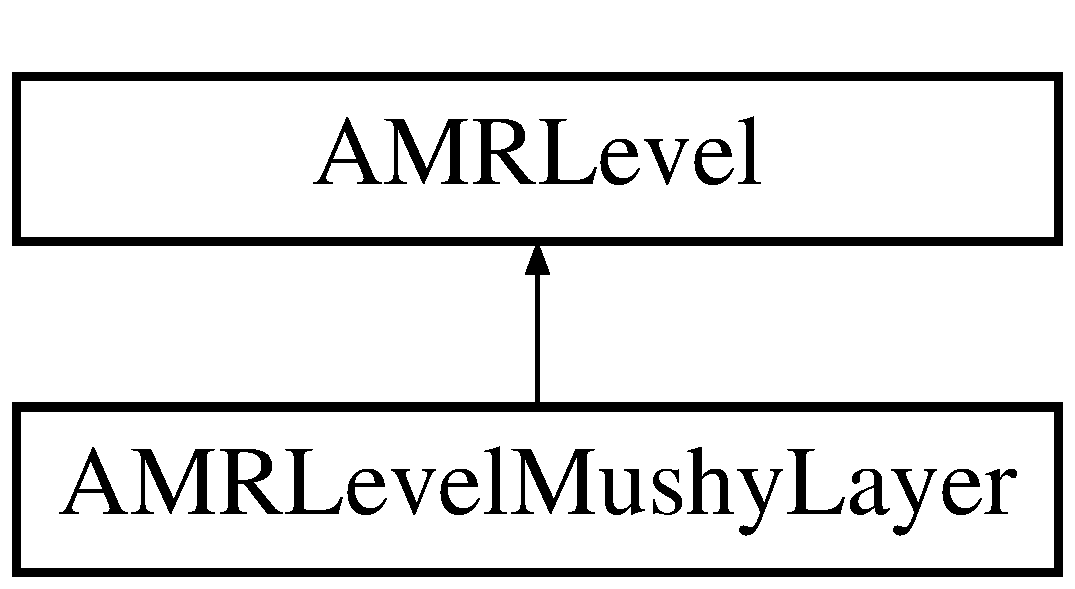
\includegraphics[height=2.000000cm]{class_a_m_r_level_mushy_layer}
\end{center}
\end{figure}
\subsection*{Public Member Functions}
\begin{DoxyCompactItemize}
\item 
\hypertarget{class_a_m_r_level_mushy_layer_adfca912f4bbd65b9d39f205a57bc651d}{\hyperlink{class_a_m_r_level_mushy_layer_adfca912f4bbd65b9d39f205a57bc651d}{A\-M\-R\-Level\-Mushy\-Layer} ()}\label{class_a_m_r_level_mushy_layer_adfca912f4bbd65b9d39f205a57bc651d}

\begin{DoxyCompactList}\small\item\em Default constructor. \end{DoxyCompactList}\item 
\hypertarget{class_a_m_r_level_mushy_layer_ad86102015982967da21a13e87f13e065}{\hyperlink{class_a_m_r_level_mushy_layer_ad86102015982967da21a13e87f13e065}{A\-M\-R\-Level\-Mushy\-Layer} (const Real \&a\-\_\-cfl, const Real \&a\-\_\-domain\-Width, const Real \&a\-\_\-refine\-Thresh, const int \&a\-\_\-tag\-Buffer\-Size, const bool \&a\-\_\-use\-Limiting)}\label{class_a_m_r_level_mushy_layer_ad86102015982967da21a13e87f13e065}

\begin{DoxyCompactList}\small\item\em Full constructor. Arguments are same as in \hyperlink{class_a_m_r_level_mushy_layer_a1510d27c94955086af90d133d3932610}{define()} \end{DoxyCompactList}\item 
void \hyperlink{class_a_m_r_level_mushy_layer_a1510d27c94955086af90d133d3932610}{define} (const Real \&a\-\_\-cfl, const Real \&a\-\_\-domain\-Width, const Real \&a\-\_\-refine\-Thresh, const int \&a\-\_\-tag\-Buffer\-Size, const bool \&a\-\_\-use\-Limiting)
\begin{DoxyCompactList}\small\item\em Defines this \hyperlink{class_a_m_r_level_mushy_layer}{A\-M\-R\-Level\-Mushy\-Layer}. \end{DoxyCompactList}\item 
\hypertarget{class_a_m_r_level_mushy_layer_a4520425f77deb76db6fd3eb789e4c68b}{virtual void \hyperlink{class_a_m_r_level_mushy_layer_a4520425f77deb76db6fd3eb789e4c68b}{define} (A\-M\-R\-Level $\ast$a\-\_\-coarser\-Level\-Ptr, const Box \&a\-\_\-problem\-Domain, int a\-\_\-level, int a\-\_\-ref\-Ratio)}\label{class_a_m_r_level_mushy_layer_a4520425f77deb76db6fd3eb789e4c68b}

\begin{DoxyCompactList}\small\item\em Never called\-: historical. \end{DoxyCompactList}\item 
\hypertarget{class_a_m_r_level_mushy_layer_a1ed163b80b24d3dc053097d24dc55be5}{virtual void \hyperlink{class_a_m_r_level_mushy_layer_a1ed163b80b24d3dc053097d24dc55be5}{define} (A\-M\-R\-Level $\ast$a\-\_\-coarser\-Level\-Ptr, const Problem\-Domain \&a\-\_\-problem\-Domain, int a\-\_\-level, int a\-\_\-ref\-Ratio)}\label{class_a_m_r_level_mushy_layer_a1ed163b80b24d3dc053097d24dc55be5}

\begin{DoxyCompactList}\small\item\em Define new \hyperlink{class_a_m_r_level_mushy_layer}{A\-M\-R\-Level\-Mushy\-Layer} from coarser. \end{DoxyCompactList}\item 
\hypertarget{class_a_m_r_level_mushy_layer_aa303a6233d0a9cf8701035e98e6d028d}{virtual Real \hyperlink{class_a_m_r_level_mushy_layer_aa303a6233d0a9cf8701035e98e6d028d}{advance} ()}\label{class_a_m_r_level_mushy_layer_aa303a6233d0a9cf8701035e98e6d028d}

\begin{DoxyCompactList}\small\item\em Advance by one timestep. \end{DoxyCompactList}\item 
\hypertarget{class_a_m_r_level_mushy_layer_a9c9c444cc77e9f623ddc9132ee4bc532}{virtual void \hyperlink{class_a_m_r_level_mushy_layer_a9c9c444cc77e9f623ddc9132ee4bc532}{post\-Time\-Step} ()}\label{class_a_m_r_level_mushy_layer_a9c9c444cc77e9f623ddc9132ee4bc532}

\begin{DoxyCompactList}\small\item\em Things to do after a timestep. \end{DoxyCompactList}\item 
\hypertarget{class_a_m_r_level_mushy_layer_a296b5accca2569adda4f91b90f0213e0}{void {\bfseries do\-Explicit\-Reflux} (int a\-\_\-var)}\label{class_a_m_r_level_mushy_layer_a296b5accca2569adda4f91b90f0213e0}

\item 
\hypertarget{class_a_m_r_level_mushy_layer_ad6c20b4a85790c49eab030f6909a0a0b}{Real {\bfseries do\-H\-Creflux} ()}\label{class_a_m_r_level_mushy_layer_ad6c20b4a85790c49eab030f6909a0a0b}

\item 
\hypertarget{class_a_m_r_level_mushy_layer_a74d98dd94e04f4732f7ac6b71e7b484c}{void {\bfseries do\-Momentum\-Reflux} (Vector$<$ Level\-Data$<$ F\-Array\-Box $>$ $\ast$ $>$ \&comp\-Vel)}\label{class_a_m_r_level_mushy_layer_a74d98dd94e04f4732f7ac6b71e7b484c}

\item 
\hypertarget{class_a_m_r_level_mushy_layer_aff274f3682a706271fc3a26eefb0be20}{virtual void \hyperlink{class_a_m_r_level_mushy_layer_aff274f3682a706271fc3a26eefb0be20}{tag\-Cells} (Int\-Vect\-Set \&a\-\_\-tags)}\label{class_a_m_r_level_mushy_layer_aff274f3682a706271fc3a26eefb0be20}

\begin{DoxyCompactList}\small\item\em Create tags for regridding. \end{DoxyCompactList}\item 
\hypertarget{class_a_m_r_level_mushy_layer_a3bfdf4f5d7260b8f6f834777ce8a7650}{void \hyperlink{class_a_m_r_level_mushy_layer_a3bfdf4f5d7260b8f6f834777ce8a7650}{tag\-Mush\-Liquid\-Boundary} (Int\-Vect\-Set \&local\-Tags)}\label{class_a_m_r_level_mushy_layer_a3bfdf4f5d7260b8f6f834777ce8a7650}

\begin{DoxyCompactList}\small\item\em Tags cells on the mush side of the mush-\/liquid boundary. \end{DoxyCompactList}\item 
\hypertarget{class_a_m_r_level_mushy_layer_a4581ecc244c826a19c696e5b8d01abf3}{void \hyperlink{class_a_m_r_level_mushy_layer_a4581ecc244c826a19c696e5b8d01abf3}{tag\-Boundary\-Layer\-Cells} (Int\-Vect\-Set \&local\-Tags)}\label{class_a_m_r_level_mushy_layer_a4581ecc244c826a19c696e5b8d01abf3}

\begin{DoxyCompactList}\small\item\em Tag cells on the domain boundary. \end{DoxyCompactList}\item 
\hypertarget{class_a_m_r_level_mushy_layer_a6eee1db20d8b07c958a1e19af1dbbe4a}{void \hyperlink{class_a_m_r_level_mushy_layer_a6eee1db20d8b07c958a1e19af1dbbe4a}{tag\-Center\-Cells} (Int\-Vect\-Set \&local\-Tags, Real radius=0)}\label{class_a_m_r_level_mushy_layer_a6eee1db20d8b07c958a1e19af1dbbe4a}

\begin{DoxyCompactList}\small\item\em Tag cells inside grid. \end{DoxyCompactList}\item 
\hypertarget{class_a_m_r_level_mushy_layer_a921f860820c88cc804345a20c2bd596d}{void \hyperlink{class_a_m_r_level_mushy_layer_a921f860820c88cc804345a20c2bd596d}{tag\-Mushy\-Cells} (Int\-Vect\-Set \&local\-Tags)}\label{class_a_m_r_level_mushy_layer_a921f860820c88cc804345a20c2bd596d}

\begin{DoxyCompactList}\small\item\em Tag cells with porosity $<$ 1. \end{DoxyCompactList}\item 
\hypertarget{class_a_m_r_level_mushy_layer_ac2a65f143504a09f92cb01907f15f124}{void \hyperlink{class_a_m_r_level_mushy_layer_ac2a65f143504a09f92cb01907f15f124}{tag\-Cells\-Var} (Int\-Vect\-Set \&local\-Tags, Real refine\-Thresh, int tagging\-Var, int vector\-Tagging\-Var, int tagging\-Method, int comp=-\/1)}\label{class_a_m_r_level_mushy_layer_ac2a65f143504a09f92cb01907f15f124}

\begin{DoxyCompactList}\small\item\em Add cells that specify criteria. \end{DoxyCompactList}\item 
void \hyperlink{class_a_m_r_level_mushy_layer_a5064704173348a8efa158f400983a101}{set\-Eta} (Real a\-\_\-eta)
\begin{DoxyCompactList}\small\item\em Set eta on all projection operators. \end{DoxyCompactList}\item 
\hypertarget{class_a_m_r_level_mushy_layer_a2771f661ce974eec626324cf2b07fd59}{Real \hyperlink{class_a_m_r_level_mushy_layer_a2771f661ce974eec626324cf2b07fd59}{max\-Allowed\-Eta} ()}\label{class_a_m_r_level_mushy_layer_a2771f661ce974eec626324cf2b07fd59}

\begin{DoxyCompactList}\small\item\em Maximum allowed eta. \end{DoxyCompactList}\item 
\hypertarget{class_a_m_r_level_mushy_layer_ac44c7ebcf787be031046fb732ac4aa96}{void \hyperlink{class_a_m_r_level_mushy_layer_ac44c7ebcf787be031046fb732ac4aa96}{set\-Adv\-Vel\-Centering} (Real a\-\_\-fraction)}\label{class_a_m_r_level_mushy_layer_ac44c7ebcf787be031046fb732ac4aa96}

\begin{DoxyCompactList}\small\item\em Set adv\-\_\-vel\-\_\-centering on all levels. \end{DoxyCompactList}\item 
\hypertarget{class_a_m_r_level_mushy_layer_a3239fcf9157c4b6174aba461e4e4b327}{virtual void \hyperlink{class_a_m_r_level_mushy_layer_a3239fcf9157c4b6174aba461e4e4b327}{tag\-Cells\-Init} (Int\-Vect\-Set \&a\-\_\-tags)}\label{class_a_m_r_level_mushy_layer_a3239fcf9157c4b6174aba461e4e4b327}

\begin{DoxyCompactList}\small\item\em Create tags at initialization. \end{DoxyCompactList}\item 
\hypertarget{class_a_m_r_level_mushy_layer_a92be42a12813c7e9bebb3ab6f025616f}{virtual void \hyperlink{class_a_m_r_level_mushy_layer_a92be42a12813c7e9bebb3ab6f025616f}{regrid} (const Vector$<$ Box $>$ \&a\-\_\-new\-Grids)}\label{class_a_m_r_level_mushy_layer_a92be42a12813c7e9bebb3ab6f025616f}

\begin{DoxyCompactList}\small\item\em Set up data on this level after regridding. \end{DoxyCompactList}\item 
\hypertarget{class_a_m_r_level_mushy_layer_adc885cc04926a87b4c4f97e3803fc749}{virtual void \hyperlink{class_a_m_r_level_mushy_layer_adc885cc04926a87b4c4f97e3803fc749}{initial\-Grid} (const Vector$<$ Box $>$ \&a\-\_\-new\-Grids)}\label{class_a_m_r_level_mushy_layer_adc885cc04926a87b4c4f97e3803fc749}

\begin{DoxyCompactList}\small\item\em Initialize grids. \end{DoxyCompactList}\item 
\hypertarget{class_a_m_r_level_mushy_layer_a7d430606668cadfa432d81d521d5cf79}{virtual void \hyperlink{class_a_m_r_level_mushy_layer_a7d430606668cadfa432d81d521d5cf79}{post\-Initial\-Grid} (const bool a\-\_\-restart)}\label{class_a_m_r_level_mushy_layer_a7d430606668cadfa432d81d521d5cf79}

\begin{DoxyCompactList}\small\item\em Operations to do after initial grids have been set up. \end{DoxyCompactList}\item 
\hypertarget{class_a_m_r_level_mushy_layer_a9b299b200bf4fadfb4ad7221177d4585}{virtual void \hyperlink{class_a_m_r_level_mushy_layer_a9b299b200bf4fadfb4ad7221177d4585}{post\-Regrid} (int a\-\_\-base\-\_\-level)}\label{class_a_m_r_level_mushy_layer_a9b299b200bf4fadfb4ad7221177d4585}

\begin{DoxyCompactList}\small\item\em Operations to execute after we've done regridding. \end{DoxyCompactList}\item 
\hypertarget{class_a_m_r_level_mushy_layer_a6763c8a7fef3e4f0c5da3c90df096e98}{void \hyperlink{class_a_m_r_level_mushy_layer_a6763c8a7fef3e4f0c5da3c90df096e98}{create\-Data\-Structures} ()}\label{class_a_m_r_level_mushy_layer_a6763c8a7fef3e4f0c5da3c90df096e98}

\begin{DoxyCompactList}\small\item\em Create structures to hold data. \end{DoxyCompactList}\item 
\hypertarget{class_a_m_r_level_mushy_layer_ac0291e7b321a6f26a057dfd2d6fb9466}{void \hyperlink{class_a_m_r_level_mushy_layer_ac0291e7b321a6f26a057dfd2d6fb9466}{init\-Data\-Structures} ()}\label{class_a_m_r_level_mushy_layer_ac0291e7b321a6f26a057dfd2d6fb9466}

\begin{DoxyCompactList}\small\item\em Initialize data structures -\/ resize arrays etc. \end{DoxyCompactList}\item 
\hypertarget{class_a_m_r_level_mushy_layer_a8dcd4deaca137c36c34b377c1f27d8af}{void {\bfseries compute\-All\-Velocities} (bool do\-F\-Rupdates)}\label{class_a_m_r_level_mushy_layer_a8dcd4deaca137c36c34b377c1f27d8af}

\item 
\hypertarget{class_a_m_r_level_mushy_layer_adae77fea47630fd1e3c2dea1c59e4c3a}{virtual void \hyperlink{class_a_m_r_level_mushy_layer_adae77fea47630fd1e3c2dea1c59e4c3a}{initial\-Data} ()}\label{class_a_m_r_level_mushy_layer_adae77fea47630fd1e3c2dea1c59e4c3a}

\begin{DoxyCompactList}\small\item\em Initialize data. \end{DoxyCompactList}\item 
\hypertarget{class_a_m_r_level_mushy_layer_ae1b467d34bd12136bab9f15b2186fd56}{void {\bfseries initial\-Data\-Corner\-Flow} ()}\label{class_a_m_r_level_mushy_layer_ae1b467d34bd12136bab9f15b2186fd56}

\item 
\hypertarget{class_a_m_r_level_mushy_layer_a3018e7aa05879f67daa66025f1a5dc02}{void {\bfseries initial\-Data\-H\-R\-L} ()}\label{class_a_m_r_level_mushy_layer_a3018e7aa05879f67daa66025f1a5dc02}

\item 
\hypertarget{class_a_m_r_level_mushy_layer_a3b71c86932fba19e9ff28e40503bc299}{void {\bfseries initial\-Data\-Convection\-Mixed\-Porous} ()}\label{class_a_m_r_level_mushy_layer_a3b71c86932fba19e9ff28e40503bc299}

\item 
\hypertarget{class_a_m_r_level_mushy_layer_a19fb2e0f21a8e3f92e6a6f4622dd9654}{void {\bfseries initial\-Data\-Poiseuille} ()}\label{class_a_m_r_level_mushy_layer_a19fb2e0f21a8e3f92e6a6f4622dd9654}

\item 
\hypertarget{class_a_m_r_level_mushy_layer_af0a22602d233dba91f217a4a2a9136b3}{void {\bfseries initial\-Data\-Ice\-Block} ()}\label{class_a_m_r_level_mushy_layer_af0a22602d233dba91f217a4a2a9136b3}

\item 
\hypertarget{class_a_m_r_level_mushy_layer_a601849adc5f5b5fc9e9999b568020922}{void {\bfseries initial\-Data\-Mushy\-Layer} ()}\label{class_a_m_r_level_mushy_layer_a601849adc5f5b5fc9e9999b568020922}

\item 
\hypertarget{class_a_m_r_level_mushy_layer_a68a589a8bddf6c0ef6a0ef4987c1e1ce}{void {\bfseries initial\-Data\-Zero\-Porosity\-Test} ()}\label{class_a_m_r_level_mushy_layer_a68a589a8bddf6c0ef6a0ef4987c1e1ce}

\item 
\hypertarget{class_a_m_r_level_mushy_layer_ab258a56bea5c0a889040d751c074f1ce}{void {\bfseries initial\-Data\-Diffusion} ()}\label{class_a_m_r_level_mushy_layer_ab258a56bea5c0a889040d751c074f1ce}

\item 
\hypertarget{class_a_m_r_level_mushy_layer_a2890289b25f3e4ea6b698ddb0d6b9223}{void {\bfseries initial\-Data\-Vortex\-Pair} ()}\label{class_a_m_r_level_mushy_layer_a2890289b25f3e4ea6b698ddb0d6b9223}

\item 
\hypertarget{class_a_m_r_level_mushy_layer_aa17f3ed72486c33689944f8c9ec5cce1}{void {\bfseries add\-Vortex} (Real\-Vect center, Real strength, Real radius)}\label{class_a_m_r_level_mushy_layer_aa17f3ed72486c33689944f8c9ec5cce1}

\item 
\hypertarget{class_a_m_r_level_mushy_layer_a376041439f9a4d8a2d62fbbd199f81f5}{void {\bfseries initial\-Data\-Rayleigh\-Benard} ()}\label{class_a_m_r_level_mushy_layer_a376041439f9a4d8a2d62fbbd199f81f5}

\item 
\hypertarget{class_a_m_r_level_mushy_layer_a36fcaecdd8d8033bdfb0d3492df1be20}{void {\bfseries initial\-Data\-Solute\-Flux} ()}\label{class_a_m_r_level_mushy_layer_a36fcaecdd8d8033bdfb0d3492df1be20}

\item 
\hypertarget{class_a_m_r_level_mushy_layer_a975f7e7062b5944e9e13c3d13fc27115}{void {\bfseries initial\-Data\-Sidewall\-Heating} ()}\label{class_a_m_r_level_mushy_layer_a975f7e7062b5944e9e13c3d13fc27115}

\item 
\hypertarget{class_a_m_r_level_mushy_layer_aeb53defbc82746d0570b7d39e6aa5b8f}{void {\bfseries initial\-Data\-Burgers} ()}\label{class_a_m_r_level_mushy_layer_aeb53defbc82746d0570b7d39e6aa5b8f}

\item 
\hypertarget{class_a_m_r_level_mushy_layer_adb8038e986c8d16f3116e267f2532409}{void {\bfseries initial\-Data\-Reflux\-Test} ()}\label{class_a_m_r_level_mushy_layer_adb8038e986c8d16f3116e267f2532409}

\item 
\hypertarget{class_a_m_r_level_mushy_layer_a0b73c4a7644eea767d6cf1d16676809d}{virtual bool \hyperlink{class_a_m_r_level_mushy_layer_a0b73c4a7644eea767d6cf1d16676809d}{converged\-To\-Steady\-State} ()}\label{class_a_m_r_level_mushy_layer_a0b73c4a7644eea767d6cf1d16676809d}

\begin{DoxyCompactList}\small\item\em Have we converged to steady state? \end{DoxyCompactList}\item 
\hypertarget{class_a_m_r_level_mushy_layer_a596d008b356f29abf0973a88136739a9}{virtual void \hyperlink{class_a_m_r_level_mushy_layer_a596d008b356f29abf0973a88136739a9}{post\-Initialize} ()}\label{class_a_m_r_level_mushy_layer_a596d008b356f29abf0973a88136739a9}

\begin{DoxyCompactList}\small\item\em Things to do after initialization. \end{DoxyCompactList}\item 
\hypertarget{class_a_m_r_level_mushy_layer_ac26973f409362a3b1aae6828737afbb3}{void \hyperlink{class_a_m_r_level_mushy_layer_ac26973f409362a3b1aae6828737afbb3}{compute\-Vorticity\-Streamfunction} ()}\label{class_a_m_r_level_mushy_layer_ac26973f409362a3b1aae6828737afbb3}

\begin{DoxyCompactList}\small\item\em Calculate vorticity and streamfunction so we can plot them. \end{DoxyCompactList}\item 
\hypertarget{class_a_m_r_level_mushy_layer_a559c35e8c90e8da2003dac3aa6cbdf8e}{void {\bfseries compute\-Vorticity} ()}\label{class_a_m_r_level_mushy_layer_a559c35e8c90e8da2003dac3aa6cbdf8e}

\item 
\hypertarget{class_a_m_r_level_mushy_layer_a318160aa2298ae805cbb19b5f2a7f750}{void {\bfseries get\-Extra\-Plot\-Fields} ()}\label{class_a_m_r_level_mushy_layer_a318160aa2298ae805cbb19b5f2a7f750}

\item 
void \hyperlink{class_a_m_r_level_mushy_layer_abedf24a1dd03d1de3c42222da1fcac3d}{write\-A\-M\-R\-Hierarchy} (string filename)
\item 
\hypertarget{class_a_m_r_level_mushy_layer_a3918643e41cb27879557d6cf06ac2f2b}{virtual Real \hyperlink{class_a_m_r_level_mushy_layer_a3918643e41cb27879557d6cf06ac2f2b}{compute\-Dt} ()}\label{class_a_m_r_level_mushy_layer_a3918643e41cb27879557d6cf06ac2f2b}

\begin{DoxyCompactList}\small\item\em Returns the dt computed earlier for this level. \end{DoxyCompactList}\item 
\hypertarget{class_a_m_r_level_mushy_layer_af9995d5aaa7f7ce624b934ba3ad9306c}{virtual Real \hyperlink{class_a_m_r_level_mushy_layer_af9995d5aaa7f7ce624b934ba3ad9306c}{compute\-Initial\-Dt} ()}\label{class_a_m_r_level_mushy_layer_af9995d5aaa7f7ce624b934ba3ad9306c}

\begin{DoxyCompactList}\small\item\em Compute dt using initial data. \end{DoxyCompactList}\item 
\hypertarget{class_a_m_r_level_mushy_layer_ac4dc44ed82584911b5d702070f493c73}{void \hyperlink{class_a_m_r_level_mushy_layer_ac4dc44ed82584911b5d702070f493c73}{compute\-Diagnostics} ()}\label{class_a_m_r_level_mushy_layer_ac4dc44ed82584911b5d702070f493c73}

\begin{DoxyCompactList}\small\item\em Compute nusselt number, salt fluxes etc. \end{DoxyCompactList}\item 
\hypertarget{class_a_m_r_level_mushy_layer_a5fc6a3c2fe287b52b6ab73d265d11cf2}{void \hyperlink{class_a_m_r_level_mushy_layer_a5fc6a3c2fe287b52b6ab73d265d11cf2}{define\-Solvers} (Real a\-\_\-time, bool a\-\_\-homogeneous=false, Real alpha=1.\-0, Real beta=1.\-0)}\label{class_a_m_r_level_mushy_layer_a5fc6a3c2fe287b52b6ab73d265d11cf2}

\begin{DoxyCompactList}\small\item\em Define solvers. \end{DoxyCompactList}\item 
\hypertarget{class_a_m_r_level_mushy_layer_af1f23fee3ffae8ab4a84caae3a87c4fc}{void {\bfseries compute\-Chimney\-Diagnostics} ()}\label{class_a_m_r_level_mushy_layer_af1f23fee3ffae8ab4a84caae3a87c4fc}

\item 
\hypertarget{class_a_m_r_level_mushy_layer_afbb2adb1dd99e2b69bcb58d5395fe3b5}{Disjoint\-Box\-Layout {\bfseries grids} ()}\label{class_a_m_r_level_mushy_layer_afbb2adb1dd99e2b69bcb58d5395fe3b5}

\item 
\hypertarget{class_a_m_r_level_mushy_layer_a03805c646cd80400874095a6960545cd}{void {\bfseries shift\-Data} (int dir, int distance)}\label{class_a_m_r_level_mushy_layer_a03805c646cd80400874095a6960545cd}

\item 
\hypertarget{class_a_m_r_level_mushy_layer_ab8b44ec14b5ddfb4d42358ae2a2f72ea}{void {\bfseries dx} (Real new\-Dx)}\label{class_a_m_r_level_mushy_layer_ab8b44ec14b5ddfb4d42358ae2a2f72ea}

\item 
\hypertarget{class_a_m_r_level_mushy_layer_a8032590f0d7a8160dc1a56151648f7c8}{void \hyperlink{class_a_m_r_level_mushy_layer_a8032590f0d7a8160dc1a56151648f7c8}{reshape\-Data} (Disjoint\-Box\-Layout new\-Grids, Problem\-Domain new\-Domain)}\label{class_a_m_r_level_mushy_layer_a8032590f0d7a8160dc1a56151648f7c8}

\begin{DoxyCompactList}\small\item\em Changed to allow changes in either x or y directions. \end{DoxyCompactList}\item 
\hypertarget{class_a_m_r_level_mushy_layer_a1afe0bf8c7646e56849d90da107afe1d}{void {\bfseries refine} (Real ref\-\_\-ratio, Disjoint\-Box\-Layout a\-\_\-grids, Problem\-Domain a\-\_\-domain)}\label{class_a_m_r_level_mushy_layer_a1afe0bf8c7646e56849d90da107afe1d}

\item 
\hypertarget{class_a_m_r_level_mushy_layer_aaeccaad92142479afdc82e3b127be495}{void \hyperlink{class_a_m_r_level_mushy_layer_aaeccaad92142479afdc82e3b127be495}{do\-Post\-Regrid\-Smoothing} (bool a\-\_\-smooth\-Vel=true, bool a\-\_\-smooth\-Scalar=true)}\label{class_a_m_r_level_mushy_layer_aaeccaad92142479afdc82e3b127be495}

\begin{DoxyCompactList}\small\item\em Do smoothing after regridding. \end{DoxyCompactList}\item 
\hypertarget{class_a_m_r_level_mushy_layer_a3c89f5bbdbe135424e8cdfd75fc03061}{void {\bfseries set\-Smoothing\-Coeff} (Real a\-\_\-coeff)}\label{class_a_m_r_level_mushy_layer_a3c89f5bbdbe135424e8cdfd75fc03061}

\item 
\hypertarget{class_a_m_r_level_mushy_layer_aca6ded080c70e8ea040576861d832e09}{void \hyperlink{class_a_m_r_level_mushy_layer_aca6ded080c70e8ea040576861d832e09}{set\-Vel\-Zero} (Level\-Data$<$ F\-Array\-Box $>$ \&a\-\_\-vel, Real a\-\_\-limit=-\/1, int a\-\_\-radius=0)}\label{class_a_m_r_level_mushy_layer_aca6ded080c70e8ea040576861d832e09}

\begin{DoxyCompactList}\small\item\em Make sure zero porosity regions have no velocity (cell centred velocity) \end{DoxyCompactList}\item 
\hypertarget{class_a_m_r_level_mushy_layer_a14cee19cc957db8f3cce3e09fca9edf3}{void \hyperlink{class_a_m_r_level_mushy_layer_a14cee19cc957db8f3cce3e09fca9edf3}{set\-Vel\-Zero} (Level\-Data$<$ Flux\-Box $>$ \&a\-\_\-vel, Real a\-\_\-limit=-\/1)}\label{class_a_m_r_level_mushy_layer_a14cee19cc957db8f3cce3e09fca9edf3}

\begin{DoxyCompactList}\small\item\em Make sure zero porosity regions have no velocity (face centred velocity) \end{DoxyCompactList}\item 
\hypertarget{class_a_m_r_level_mushy_layer_ae3dcf62f2464245d7a3035cd1508061f}{void {\bfseries set\-C\-C\-Vel\-Zero} (Real a\-\_\-limit)}\label{class_a_m_r_level_mushy_layer_ae3dcf62f2464245d7a3035cd1508061f}

\item 
\hypertarget{class_a_m_r_level_mushy_layer_a8679a53e5cbddc3af173ea3ff5b574de}{void \hyperlink{class_a_m_r_level_mushy_layer_a8679a53e5cbddc3af173ea3ff5b574de}{update\-Enthalpy\-Variables} ()}\label{class_a_m_r_level_mushy_layer_a8679a53e5cbddc3af173ea3ff5b574de}

\begin{DoxyCompactList}\small\item\em Update thermodynamic variables based on phase diagram. \end{DoxyCompactList}\item 
\hypertarget{class_a_m_r_level_mushy_layer_a2e827a3ed1a3ced10f1b47bb0014731b}{void \hyperlink{class_a_m_r_level_mushy_layer_a2e827a3ed1a3ced10f1b47bb0014731b}{compute\-Lambda\-Porosity} ()}\label{class_a_m_r_level_mushy_layer_a2e827a3ed1a3ced10f1b47bb0014731b}

\begin{DoxyCompactList}\small\item\em Compute lambda/porosity. \end{DoxyCompactList}\end{DoxyCompactItemize}
\subsection*{Public Attributes}
\begin{DoxyCompactItemize}
\item 
\hypertarget{class_a_m_r_level_mushy_layer_a280fdf87f2f58ddc25250fff6b6c9f19}{\hyperlink{class_diagnostics}{Diagnostics} \hyperlink{class_a_m_r_level_mushy_layer_a280fdf87f2f58ddc25250fff6b6c9f19}{m\-\_\-diagnostics}}\label{class_a_m_r_level_mushy_layer_a280fdf87f2f58ddc25250fff6b6c9f19}

\begin{DoxyCompactList}\small\item\em \hyperlink{class_diagnostics}{Diagnostics} e.\-g. Nusselt number, solute flux. \end{DoxyCompactList}\item 
\hypertarget{class_a_m_r_level_mushy_layer_afd5628964f3f9b398facc7098e27945b}{bool {\bfseries m\-\_\-compute\-Diagnostics}}\label{class_a_m_r_level_mushy_layer_afd5628964f3f9b398facc7098e27945b}

\end{DoxyCompactItemize}
\subsection*{Protected Types}
\begin{DoxyCompactItemize}
\item 
enum \hyperlink{class_a_m_r_level_mushy_layer_a664250846ba0de6313177ed258c1d9f4}{scalar\-Vars} \{ \\*
{\bfseries m\-\_\-enthalpy}, 
{\bfseries m\-\_\-bulk\-Concentration}, 
{\bfseries m\-\_\-temperature}, 
{\bfseries m\-\_\-porosity}, 
\\*
{\bfseries m\-\_\-liquid\-Concentration}, 
{\bfseries m\-\_\-solid\-Concentration}, 
{\bfseries m\-\_\-pressure}, 
{\bfseries m\-\_\-permeability}, 
\\*
{\bfseries m\-\_\-lambda}, 
{\bfseries m\-\_\-lambda\-\_\-porosity}, 
{\bfseries m\-\_\-enthalpy\-Solidus}, 
{\bfseries m\-\_\-enthalpy\-Liquidus}, 
\\*
{\bfseries m\-\_\-enthalpy\-Eutectic}, 
{\bfseries m\-\_\-porosity\-Analytic}, 
{\bfseries m\-\_\-temperature\-Analytic}, 
{\bfseries m\-\_\-salt\-Eqn\-Src\-Godunov}, 
\\*
{\bfseries m\-\_\-salt\-Eqn\-Src\-Finite\-Diff}, 
{\bfseries m\-\_\-salt\-Eqn\-Op}, 
{\bfseries m\-\_\-\-Terr}, 
{\bfseries m\-\_\-enthalpy\-Op}, 
\\*
{\bfseries m\-\_\-enthalpy\-Src}, 
{\bfseries m\-\_\-div\-Uadv}, 
{\bfseries m\-\_\-d\-Hdt}, 
{\bfseries m\-\_\-d\-Sdt}, 
\\*
{\bfseries m\-\_\-average\-Vertical\-Flux}, 
{\bfseries m\-\_\-solute\-Flux\-Analytic}, 
{\bfseries m\-\_\-vertical\-Flux}, 
{\bfseries m\-\_\-salt\-Residual}, 
\\*
{\bfseries m\-\_\-div\-U}, 
{\bfseries m\-\_\-average\-Heat\-Flux}, 
{\bfseries m\-\_\-streamfunction}, 
{\bfseries m\-\_\-vorticity}, 
\\*
{\bfseries m\-\_\-\-Fs\-Vert\-Diffusion}, 
{\bfseries m\-\_\-\-Fs\-Vert\-Fluid}, 
{\bfseries m\-\_\-\-Fs\-Vert\-Frame}, 
{\bfseries m\-\_\-div\-Ucorr}, 
\\*
{\bfseries m\-\_\-pi}, 
{\bfseries m\-\_\-phi}, 
{\bfseries m\-\_\-\-M\-A\-C\-B\-C}, 
{\bfseries m\-\_\-\-M\-A\-Crhs}, 
\\*
{\bfseries m\-\_\-\-C\-Crhs}, 
{\bfseries m\-\_\-num\-Scalar\-Vars}
 \}
\begin{DoxyCompactList}\small\item\em Identifiers for different scalar variables. \end{DoxyCompactList}\item 
enum \hyperlink{class_a_m_r_level_mushy_layer_ac7a25361b1895a85f5916a1adfd3153b}{vector\-Vars} \{ \\*
{\bfseries m\-\_\-fluid\-Vel}, 
{\bfseries m\-\_\-\-U\-\_\-porosity}, 
{\bfseries m\-\_\-\-Ustar}, 
{\bfseries m\-\_\-adv\-Ustar}, 
\\*
{\bfseries m\-\_\-advection\-Vel}, 
{\bfseries m\-\_\-viscous\-Solve\-Src}, 
{\bfseries m\-\_\-\-Udel\-U}, 
{\bfseries m\-\_\-advection\-Src}, 
\\*
{\bfseries m\-\_\-fluid\-Vel\-Analytic}, 
{\bfseries m\-\_\-fluid\-Vel\-Err}, 
{\bfseries m\-\_\-d\-Udt}, 
{\bfseries m\-\_\-\-Fs\-Diffusion}, 
\\*
{\bfseries m\-\_\-\-Fs\-Fluid}, 
{\bfseries m\-\_\-\-Fs}, 
{\bfseries m\-\_\-freestream\-Correction}, 
{\bfseries m\-\_\-\-Upre\-Projection}, 
\\*
{\bfseries m\-\_\-advection\-Implicit\-Src}, 
{\bfseries m\-\_\-\-M\-A\-Ccorrection}, 
{\bfseries m\-\_\-\-C\-Ccorrection}, 
{\bfseries m\-\_\-adv\-Src\-Lap\-U}, 
\\*
{\bfseries m\-\_\-adv\-Upre\-Projection}, 
{\bfseries m\-\_\-body\-Force}, 
{\bfseries m\-\_\-adv\-Vel\-Corr}, 
{\bfseries m\-\_\-num\-Vector\-Vars}
 \}
\begin{DoxyCompactList}\small\item\em Identifiers for vector variables. \end{DoxyCompactList}\item 
enum \hyperlink{class_a_m_r_level_mushy_layer_ac96810ce869ac7ad58404b43a823cba3}{M\-Gmethod} \{ \hyperlink{class_a_m_r_level_mushy_layer_ac96810ce869ac7ad58404b43a823cba3a7fcd73cadaa66126997b4e1183712951}{m\-\_\-standard}, 
\hyperlink{class_a_m_r_level_mushy_layer_ac96810ce869ac7ad58404b43a823cba3a2b0b946b439cf26fb2ee3648f4ea7744}{m\-\_\-\-F\-A\-S}
 \}
\begin{DoxyCompactList}\small\item\em Different multigrid methods. \end{DoxyCompactList}\item 
enum \hyperlink{class_a_m_r_level_mushy_layer_ae580be53bf92a5bad64ba0032282458b}{solver\-Restart} \{ {\bfseries m\-\_\-restart\-Halve\-Dt}, 
{\bfseries m\-\_\-restart\-Reset\-Data}
 \}
\begin{DoxyCompactList}\small\item\em What to do when restarting after a failed timestep. \end{DoxyCompactList}\item 
enum {\bfseries velocity\-Advection\-Types} \{ {\bfseries m\-\_\-porosity\-In\-Advection}, 
{\bfseries m\-\_\-porosity\-Outside\-Advection}, 
{\bfseries m\-\_\-no\-Porosity}
 \}
\end{DoxyCompactItemize}
\subsection*{Protected Member Functions}
\begin{DoxyCompactItemize}
\item 
\hypertarget{class_a_m_r_level_mushy_layer_aad8e3d2cda90acb68c1086e0e08096a6}{Real \hyperlink{class_a_m_r_level_mushy_layer_aad8e3d2cda90acb68c1086e0e08096a6}{converged\-To\-Steady\-State} (const int a\-\_\-var, bool vector=false)}\label{class_a_m_r_level_mushy_layer_aad8e3d2cda90acb68c1086e0e08096a6}

\begin{DoxyCompactList}\small\item\em Has a particular variable converged to steady state? \end{DoxyCompactList}\item 
\hypertarget{class_a_m_r_level_mushy_layer_a0f76ac50feba2ebcf8cd431948690a76}{void {\bfseries compute\-\_\-d\-\_\-dt} (const int a\-\_\-var, Level\-Data$<$ F\-Array\-Box $>$ \&diff, bool vector=false)}\label{class_a_m_r_level_mushy_layer_a0f76ac50feba2ebcf8cd431948690a76}

\item 
\hypertarget{class_a_m_r_level_mushy_layer_ab86dcb9c77a0696fbb3fbc7d6a1d09b3}{bool \hyperlink{class_a_m_r_level_mushy_layer_ab86dcb9c77a0696fbb3fbc7d6a1d09b3}{solving\-Full\-Darcy\-Brinkman} ()}\label{class_a_m_r_level_mushy_layer_ab86dcb9c77a0696fbb3fbc7d6a1d09b3}

\begin{DoxyCompactList}\small\item\em Determine if we're solving the full time dependent equation, or just darcy's law. \end{DoxyCompactList}\item 
\hypertarget{class_a_m_r_level_mushy_layer_a540bac726905fcc0af2fcfe7a8b7fed1}{void \hyperlink{class_a_m_r_level_mushy_layer_a540bac726905fcc0af2fcfe7a8b7fed1}{update\-Enthalpy\-Variables\-Old} ()}\label{class_a_m_r_level_mushy_layer_a540bac726905fcc0af2fcfe7a8b7fed1}

\begin{DoxyCompactList}\small\item\em Update thermodynamic variables based on phase diagram (old time) \end{DoxyCompactList}\item 
\hypertarget{class_a_m_r_level_mushy_layer_ad978d1a9a28c1ef557aa348807534eb4}{bool \hyperlink{class_a_m_r_level_mushy_layer_ad978d1a9a28c1ef557aa348807534eb4}{finest\-Level} ()}\label{class_a_m_r_level_mushy_layer_ad978d1a9a28c1ef557aa348807534eb4}

\begin{DoxyCompactList}\small\item\em Returns true if there is not a finer level with a grid defined on it. \end{DoxyCompactList}\item 
\hypertarget{class_a_m_r_level_mushy_layer_a52cfb93ecc1e44063a1db80fb417017b}{int \hyperlink{class_a_m_r_level_mushy_layer_a52cfb93ecc1e44063a1db80fb417017b}{get\-Finest\-Level} ()}\label{class_a_m_r_level_mushy_layer_a52cfb93ecc1e44063a1db80fb417017b}

\begin{DoxyCompactList}\small\item\em Return the finest level. \end{DoxyCompactList}\item 
\hypertarget{class_a_m_r_level_mushy_layer_a38c3d474a125f8cf66dd07e08ee02709}{Real \hyperlink{class_a_m_r_level_mushy_layer_a38c3d474a125f8cf66dd07e08ee02709}{compute\-Dt} (Real cfl)}\label{class_a_m_r_level_mushy_layer_a38c3d474a125f8cf66dd07e08ee02709}

\begin{DoxyCompactList}\small\item\em Returns $ \Delta t $. \end{DoxyCompactList}\item 
\hypertarget{class_a_m_r_level_mushy_layer_aa758dba965ec2072e89a8bb75620db1b}{Real {\bfseries get\-Max\-Velocity} ()}\label{class_a_m_r_level_mushy_layer_aa758dba965ec2072e89a8bb75620db1b}

\item 
\hypertarget{class_a_m_r_level_mushy_layer_a3eee3de4d8921d0778ed037698c5d5c4}{Real \hyperlink{class_a_m_r_level_mushy_layer_a3eee3de4d8921d0778ed037698c5d5c4}{compute\-Dt} (bool growdt)}\label{class_a_m_r_level_mushy_layer_a3eee3de4d8921d0778ed037698c5d5c4}

\begin{DoxyCompactList}\small\item\em Returns $ \Delta t $. \end{DoxyCompactList}\item 
\hypertarget{class_a_m_r_level_mushy_layer_aa98ba6180396656e312b6449f4ebd8eb}{void \hyperlink{class_a_m_r_level_mushy_layer_aa98ba6180396656e312b6449f4ebd8eb}{compute\-Salt\-Residual} (Level\-Data$<$ Flux\-Box $>$ \&total\-Solute\-Flux)}\label{class_a_m_r_level_mushy_layer_aa98ba6180396656e312b6449f4ebd8eb}

\begin{DoxyCompactList}\small\item\em Compute salt equation residual. \end{DoxyCompactList}\item 
\hypertarget{class_a_m_r_level_mushy_layer_adaba898a184c0cd44d6d1b12f52ef503}{void \hyperlink{class_a_m_r_level_mushy_layer_adaba898a184c0cd44d6d1b12f52ef503}{restart\-Timestep\-From\-Backup} (bool ignore\-Pressure=false)}\label{class_a_m_r_level_mushy_layer_adaba898a184c0cd44d6d1b12f52ef503}

\begin{DoxyCompactList}\small\item\em Replace with data from before the last backup. \end{DoxyCompactList}\item 
\hypertarget{class_a_m_r_level_mushy_layer_a165220ab8589f345f78556bf427e3745}{void \hyperlink{class_a_m_r_level_mushy_layer_a165220ab8589f345f78556bf427e3745}{backup\-Timestep} ()}\label{class_a_m_r_level_mushy_layer_a165220ab8589f345f78556bf427e3745}

\begin{DoxyCompactList}\small\item\em Save the current data. \end{DoxyCompactList}\item 
\hypertarget{class_a_m_r_level_mushy_layer_a2c8c30594b0753f915713ca0e701eb3a}{void \hyperlink{class_a_m_r_level_mushy_layer_a2c8c30594b0753f915713ca0e701eb3a}{get\-Hierarchy\-And\-Grids} (Vector$<$ \hyperlink{class_a_m_r_level_mushy_layer}{A\-M\-R\-Level\-Mushy\-Layer} $\ast$ $>$ \&a\-\_\-hierarchy, Vector$<$ Disjoint\-Box\-Layout $>$ \&a\-\_\-grids, Vector$<$ int $>$ \&a\-\_\-ref\-Rat, Problem\-Domain \&a\-\_\-lev0\-Dom, Real \&a\-\_\-lev0\-Dx)}\label{class_a_m_r_level_mushy_layer_a2c8c30594b0753f915713ca0e701eb3a}

\begin{DoxyCompactList}\small\item\em Get information on the entire A\-M\-R hierarchy. \end{DoxyCompactList}\item 
\hypertarget{class_a_m_r_level_mushy_layer_aef9f77f57da892bd8930943bfbec9a6b}{void \hyperlink{class_a_m_r_level_mushy_layer_aef9f77f57da892bd8930943bfbec9a6b}{calculate\-Permeability} ()}\label{class_a_m_r_level_mushy_layer_aef9f77f57da892bd8930943bfbec9a6b}

\begin{DoxyCompactList}\small\item\em Calculate permeability $ \Pi $. \end{DoxyCompactList}\item 
\hypertarget{class_a_m_r_level_mushy_layer_a3b0111c15c91c012d328e42b43fa954f}{void \hyperlink{class_a_m_r_level_mushy_layer_a3b0111c15c91c012d328e42b43fa954f}{calculate\-Coarse\-Fine\-Boundaries} (int a\-\_\-var, bool vector=false)}\label{class_a_m_r_level_mushy_layer_a3b0111c15c91c012d328e42b43fa954f}

\begin{DoxyCompactList}\small\item\em Fills coarse-\/fine boundaries on variable by quadratic interpolation. \end{DoxyCompactList}\item 
int \hyperlink{class_a_m_r_level_mushy_layer_adc086e9a094b35435de36aadb3891ab7}{multi\-Comp\-Advect\-Diffuse} (Level\-Data$<$ F\-Array\-Box $>$ \&a\-\_\-phi\-\_\-old, Level\-Data$<$ F\-Array\-Box $>$ \&a\-\_\-phi\-\_\-new, Level\-Data$<$ F\-Array\-Box $>$ \&a\-\_\-src, bool do\-F\-Rupdates=false, bool compute\-Advective\-Src=true)
\begin{DoxyCompactList}\small\item\em Advect and diffuse a scalar field. Returns multigrid status. \end{DoxyCompactList}\item 
\hypertarget{class_a_m_r_level_mushy_layer_af640c8b9d905e16e6b90b6c4f1c7fda2}{void \hyperlink{class_a_m_r_level_mushy_layer_af640c8b9d905e16e6b90b6c4f1c7fda2}{compute\-Scalar\-Advective\-Src} (Level\-Data$<$ F\-Array\-Box $>$ \&a\-\_\-src, int a\-\_\-var, bool converged, int a\-\_\-comp=0)}\label{class_a_m_r_level_mushy_layer_af640c8b9d905e16e6b90b6c4f1c7fda2}

\begin{DoxyCompactList}\small\item\em Compute src term and add it to a\-\_\-src. \end{DoxyCompactList}\item 
\hypertarget{class_a_m_r_level_mushy_layer_ab376d561af9e6d98881d71bb00184b7f}{void \hyperlink{class_a_m_r_level_mushy_layer_ab376d561af9e6d98881d71bb00184b7f}{compute\-Scalar\-Advective\-Src\-H\-C} (Level\-Data$<$ F\-Array\-Box $>$ \&a\-\_\-src, Level\-Data$<$ Flux\-Box $>$ \&edge\-Scal\-Total, bool converged)}\label{class_a_m_r_level_mushy_layer_ab376d561af9e6d98881d71bb00184b7f}

\begin{DoxyCompactList}\small\item\em Compute multi component source term\-: $ (\mathbf{U} \cdot \nabla T, \mathbf{U} \cdot \nabla S_l)$. \end{DoxyCompactList}\item 
\hypertarget{class_a_m_r_level_mushy_layer_a3ea7646ada59f1476523b7a71fa7c40d}{void {\bfseries increment\-Flux\-Registers} (Level\-Data$<$ Flux\-Box $>$ \&flux, Real flux\-Mult)}\label{class_a_m_r_level_mushy_layer_a3ea7646ada59f1476523b7a71fa7c40d}

\item 
void \hyperlink{class_a_m_r_level_mushy_layer_a8f04027bc844bd17a8bed1e073978436}{compute\-Total\-Advective\-Fluxes} (Level\-Data$<$ Flux\-Box $>$ \&edge\-Scal\-Total)
\begin{DoxyCompactList}\small\item\em Compute total fluxes that provide the source term for implicit enthalpy-\/salinity updates. \end{DoxyCompactList}\item 
void \hyperlink{class_a_m_r_level_mushy_layer_a367dd316723860bb7bd1c8b97895a3f4}{advect\-Scalar} (const int a\-\_\-scalar\-Var, const int a\-\_\-advection\-Var, Level\-Data$<$ Flux\-Box $>$ \&a\-\_\-adv\-Vel, bool do\-F\-Rupdates=true)
\begin{DoxyCompactList}\small\item\em Update a scalar field by advection. \end{DoxyCompactList}\item 
\hypertarget{class_a_m_r_level_mushy_layer_aec550a75ccdfb94eef6efb396228f075}{void {\bfseries advect\-Scalar} (const int a\-\_\-scalar\-Var, const int a\-\_\-advection\-Var, Level\-Data$<$ Flux\-Box $>$ \&a\-\_\-adv\-Vel, bool do\-F\-Rupdates, Level\-Data$<$ Flux\-Box $>$ \&flux)}\label{class_a_m_r_level_mushy_layer_aec550a75ccdfb94eef6efb396228f075}

\item 
\hypertarget{class_a_m_r_level_mushy_layer_a0d28eb0d78389d0fc13f0b6c69b8157b}{void {\bfseries update\-Scalar\-Flux\-Register} (int a\-\_\-scalar\-Var, Level\-Data$<$ Flux\-Box $>$ \&flux, Real scale)}\label{class_a_m_r_level_mushy_layer_a0d28eb0d78389d0fc13f0b6c69b8157b}

\item 
void \hyperlink{class_a_m_r_level_mushy_layer_acfd7a12794a564615d7b507717ea0d70}{advect\-Lambda} (bool do\-F\-Rupdates=true)
\begin{DoxyCompactList}\small\item\em Advect lambda field (for freestream preservation) \end{DoxyCompactList}\item 
void \hyperlink{class_a_m_r_level_mushy_layer_a4c5ae9f4b8016a17944e103389ac6c1f}{compute\-Advection\-Vel\-Source\-Term} (Level\-Data$<$ F\-Array\-Box $>$ \&advection\-Source\-Term)
\begin{DoxyCompactList}\small\item\em Time integration by the T\-G\-A method (2nd order accurate) \end{DoxyCompactList}\item 
\hypertarget{class_a_m_r_level_mushy_layer_a51a93e1db4963170b0cc831bf87bdbda}{void \hyperlink{class_a_m_r_level_mushy_layer_a51a93e1db4963170b0cc831bf87bdbda}{horizontally\-Average} (Level\-Data$<$ F\-Array\-Box $>$ \&a\-\_\-averaged, Level\-Data$<$ Flux\-Box $>$ \&a\-\_\-phi)}\label{class_a_m_r_level_mushy_layer_a51a93e1db4963170b0cc831bf87bdbda}

\begin{DoxyCompactList}\small\item\em Average vertical fluxes in the horizontal direction. \end{DoxyCompactList}\item 
\hypertarget{class_a_m_r_level_mushy_layer_a59d164085c308e534cdb44f558c56aed}{void {\bfseries horizontally\-Average} (Vector$<$ Real $>$ \&average\-Vector, Level\-Data$<$ Flux\-Box $>$ \&a\-\_\-phi)}\label{class_a_m_r_level_mushy_layer_a59d164085c308e534cdb44f558c56aed}

\item 
\hypertarget{class_a_m_r_level_mushy_layer_ace588d01606542a417a8d2d05c80c392}{void {\bfseries horizontally\-Average} (Level\-Data$<$ F\-Array\-Box $>$ \&a\-\_\-averaged, Level\-Data$<$ Flux\-Box $>$ \&a\-\_\-phi, Vector$<$ Real $>$ \&average\-Vector)}\label{class_a_m_r_level_mushy_layer_ace588d01606542a417a8d2d05c80c392}

\item 
\hypertarget{class_a_m_r_level_mushy_layer_a4467aac78f7a23f22a7d65d3441ffb8b}{void \hyperlink{class_a_m_r_level_mushy_layer_a4467aac78f7a23f22a7d65d3441ffb8b}{horizontally\-Average} (Level\-Data$<$ F\-Array\-Box $>$ \&a\-\_\-averaged, Level\-Data$<$ F\-Array\-Box $>$ \&a\-\_\-phi)}\label{class_a_m_r_level_mushy_layer_a4467aac78f7a23f22a7d65d3441ffb8b}

\begin{DoxyCompactList}\small\item\em Average vertical fluxes in the horizontal direction. \end{DoxyCompactList}\item 
\hypertarget{class_a_m_r_level_mushy_layer_a56619b718d89610566ede8f9a6f74270}{void {\bfseries horizontally\-Average} (Vector$<$ Real $>$ \&average\-Vector, Level\-Data$<$ F\-Array\-Box $>$ \&a\-\_\-phi)}\label{class_a_m_r_level_mushy_layer_a56619b718d89610566ede8f9a6f74270}

\item 
\hypertarget{class_a_m_r_level_mushy_layer_af2c7dbb0a17702772ed44fd557aff2ae}{void {\bfseries horizontally\-Average} (Level\-Data$<$ F\-Array\-Box $>$ \&a\-\_\-averaged, Level\-Data$<$ F\-Array\-Box $>$ \&a\-\_\-phi, Vector$<$ Real $>$ \&global\-Averaged)}\label{class_a_m_r_level_mushy_layer_af2c7dbb0a17702772ed44fd557aff2ae}

\item 
\hypertarget{class_a_m_r_level_mushy_layer_a7173a5848825f83a3692ff35bcb91631}{Real {\bfseries average\-Over\-Liquid\-Region} (int a\-\_\-val)}\label{class_a_m_r_level_mushy_layer_a7173a5848825f83a3692ff35bcb91631}

\item 
\hypertarget{class_a_m_r_level_mushy_layer_a6741ef0d7091e2c65c4e4b9f9d5a172a}{void {\bfseries get\-Total\-Flux} (Level\-Data$<$ Flux\-Box $>$ \&total\-Flux)}\label{class_a_m_r_level_mushy_layer_a6741ef0d7091e2c65c4e4b9f9d5a172a}

\item 
\hypertarget{class_a_m_r_level_mushy_layer_a4a641297a46991e7aca4ab750b347a1f}{void \hyperlink{class_a_m_r_level_mushy_layer_a4a641297a46991e7aca4ab750b347a1f}{compute\-Lap\-Vel} (Level\-Data$<$ F\-Array\-Box $>$ \&a\-\_\-lap\-Vel, Level\-Data$<$ F\-Array\-Box $>$ \&a\-\_\-vel, const Level\-Data$<$ F\-Array\-Box $>$ $\ast$a\-\_\-crse\-Vel\-Ptr)}\label{class_a_m_r_level_mushy_layer_a4a641297a46991e7aca4ab750b347a1f}

\begin{DoxyCompactList}\small\item\em Compute $ \nabla^2 \mathbf{U} $. \end{DoxyCompactList}\item 
\hypertarget{class_a_m_r_level_mushy_layer_ae23a8e865baef2bc23d79e7839c2a31b}{void \hyperlink{class_a_m_r_level_mushy_layer_ae23a8e865baef2bc23d79e7839c2a31b}{compute\-Scal\-Diffusion} (const int a\-\_\-var, Level\-Data$<$ F\-Array\-Box $>$ \&a\-\_\-lap\-Scal, Real a\-\_\-time)}\label{class_a_m_r_level_mushy_layer_ae23a8e865baef2bc23d79e7839c2a31b}

\begin{DoxyCompactList}\small\item\em Compute $ \nabla^2 \phi $. \end{DoxyCompactList}\item 
\hypertarget{class_a_m_r_level_mushy_layer_a00dc47be23a770c7a546a2b79a7bcf5c}{void \hyperlink{class_a_m_r_level_mushy_layer_a00dc47be23a770c7a546a2b79a7bcf5c}{compute\-Scal\-Diffusion} (Level\-Data$<$ F\-Array\-Box $>$ \&diffusive\-Src, Real a\-\_\-time)}\label{class_a_m_r_level_mushy_layer_a00dc47be23a770c7a546a2b79a7bcf5c}

\begin{DoxyCompactList}\small\item\em Compute $ \nabla^2 (H, S) $. \end{DoxyCompactList}\item 
\hypertarget{class_a_m_r_level_mushy_layer_a9af796bb0c94d60cb54d97c3c935bfdf}{void {\bfseries compute\-Scal\-Diffusion} (Level\-Data$<$ F\-Array\-Box $>$ \&a\-\_\-src, int a\-\_\-var)}\label{class_a_m_r_level_mushy_layer_a9af796bb0c94d60cb54d97c3c935bfdf}

\item 
\hypertarget{class_a_m_r_level_mushy_layer_add5a2303e20f8efa62a09005dc48bc6d}{void {\bfseries compute\-C\-Cvelocity} (Level\-Data$<$ F\-Array\-Box $>$ \&advection\-Source\-Term, Real a\-\_\-old\-Time, Real a\-\_\-dt, bool do\-F\-Rupdates=false, bool a\-\_\-do\-Projection=true, bool compute\-\_\-u\-Del\-U=true, bool a\-\_\-\-M\-A\-Cprojection=false)}\label{class_a_m_r_level_mushy_layer_add5a2303e20f8efa62a09005dc48bc6d}

\item 
\hypertarget{class_a_m_r_level_mushy_layer_a059eedd6197f85a0d1638ca6183295d4}{void \hyperlink{class_a_m_r_level_mushy_layer_a059eedd6197f85a0d1638ca6183295d4}{compute\-Ustar} (Level\-Data$<$ F\-Array\-Box $>$ \&a\-\_\-u\-Delu, Real a\-\_\-old\-Time, Real a\-\_\-dt, bool do\-F\-Rupdates, bool a\-\_\-\-M\-A\-Cprojection=false)}\label{class_a_m_r_level_mushy_layer_a059eedd6197f85a0d1638ca6183295d4}

\begin{DoxyCompactList}\small\item\em Compute $ \mathbf{U}^* $, the velocity before we project it. \end{DoxyCompactList}\item 
\hypertarget{class_a_m_r_level_mushy_layer_aeaec7664c5366f241354c00436e4a87f}{void \hyperlink{class_a_m_r_level_mushy_layer_aeaec7664c5366f241354c00436e4a87f}{compute\-Ustar\-Src} (Level\-Data$<$ F\-Array\-Box $>$ \&src, Level\-Data$<$ F\-Array\-Box $>$ \&a\-\_\-u\-Delu, Real src\-\_\-time, bool a\-\_\-\-M\-A\-Cprojection=false)}\label{class_a_m_r_level_mushy_layer_aeaec7664c5366f241354c00436e4a87f}

\begin{DoxyCompactList}\small\item\em Compute the source term for the $\mathbf{U}^* $ solve. \end{DoxyCompactList}\item 
\hypertarget{class_a_m_r_level_mushy_layer_a1699a841bc8d8371f55c6ac45152d4ea}{void \hyperlink{class_a_m_r_level_mushy_layer_a1699a841bc8d8371f55c6ac45152d4ea}{set\-Vel\-Zero} (F\-Array\-Box \&a\-\_\-vel, const F\-Array\-Box \&a\-\_\-porosity, const Real a\-\_\-limit, const int a\-\_\-radius=0)}\label{class_a_m_r_level_mushy_layer_a1699a841bc8d8371f55c6ac45152d4ea}

\begin{DoxyCompactList}\small\item\em F\-A\-B version. \end{DoxyCompactList}\item 
\hypertarget{class_a_m_r_level_mushy_layer_ad1e22532941e086464363b556c60b82c}{void \hyperlink{class_a_m_r_level_mushy_layer_ad1e22532941e086464363b556c60b82c}{compute\-Grad\-P} (Level\-Data$<$ F\-Array\-Box $>$ \&grad\-P, Real a\-\_\-time, bool a\-\_\-mac\-Projection=false)}\label{class_a_m_r_level_mushy_layer_ad1e22532941e086464363b556c60b82c}

\begin{DoxyCompactList}\small\item\em Returns $ \nabla P $ at the specified time. \end{DoxyCompactList}\item 
\hypertarget{class_a_m_r_level_mushy_layer_a1da14630642f32edf8ab0c3d27ecf60e}{void \hyperlink{class_a_m_r_level_mushy_layer_a1da14630642f32edf8ab0c3d27ecf60e}{trace\-Advection\-Vel} (Level\-Data$<$ Flux\-Box $>$ \&a\-\_\-adv\-Vel, Level\-Data$<$ F\-Array\-Box $>$ \&a\-\_\-old\-\_\-vel, Level\-Data$<$ F\-Array\-Box $>$ \&U\-\_\-chi, const Level\-Data$<$ F\-Array\-Box $>$ \&a\-\_\-viscous\-Source, Patch\-Godunov \&a\-\_\-patch\-God\-Velocity, Real a\-\_\-old\-\_\-time, Real a\-\_\-dt)}\label{class_a_m_r_level_mushy_layer_a1da14630642f32edf8ab0c3d27ecf60e}

\begin{DoxyCompactList}\small\item\em Trace the advection velocity forward in time. \end{DoxyCompactList}\item 
\hypertarget{class_a_m_r_level_mushy_layer_a93fde307e987b4d1e5dbdb06b29d23d0}{void \hyperlink{class_a_m_r_level_mushy_layer_a93fde307e987b4d1e5dbdb06b29d23d0}{compute\-Predicted\-Velocities} (Level\-Data$<$ Flux\-Box $>$ \&U\-\_\-chi\-\_\-new, Level\-Data$<$ F\-Array\-Box $>$ \&a\-\_\-trace\-Vel, Level\-Data$<$ Flux\-Box $>$ \&a\-\_\-adv\-Vel, Level\-Data$<$ F\-Array\-Box $>$ \&U\-\_\-chi, Level\-Data$<$ F\-Array\-Box $>$ \&a\-\_\-viscous\-Source, Patch\-Godunov \&a\-\_\-patch\-God\-Velocity, Level\-Data$<$ Flux\-Box $>$ \&a\-\_\-grad\-\_\-e\-Lambda, Level\-Data$<$ Flux\-Box $>$ \&a\-\_\-grad\-Phi, Level\-Data$<$ Flux\-Box $>$ \&porosity\-Face, Real a\-\_\-old\-\_\-time, Real a\-\_\-dt, bool legacy\-Compute=false)}\label{class_a_m_r_level_mushy_layer_a93fde307e987b4d1e5dbdb06b29d23d0}

\begin{DoxyCompactList}\small\item\em Compute advection velocities at the half time step. \end{DoxyCompactList}\item 
void \hyperlink{class_a_m_r_level_mushy_layer_a77914a8f6be67642c366b4da8e0a2829}{compute\-Scalar\-Advective\-Flux} (Level\-Data$<$ Flux\-Box $>$ \&a\-\_\-edge\-Scal, Level\-Data$<$ F\-Array\-Box $>$ \&a\-\_\-old\-\_\-scal, Level\-Data$<$ Flux\-Box $>$ \&a\-\_\-adv\-\_\-vel, Level\-Data$<$ Flux\-Box $>$ \&a\-\_\-inflow\-Outflow\-Vel, Level\-Data$<$ F\-Array\-Box $>$ \&a\-\_\-old\-\_\-vel, Level\-Data$<$ F\-Array\-Box $>$ \&a\-\_\-diffusive\-Src, Patch\-Godunov \&a\-\_\-patch\-God, Real a\-\_\-old\-\_\-time, Real a\-\_\-dt)
\begin{DoxyCompactList}\small\item\em Compute the advective flux given the scalar field, advection velocity and source term specified. \end{DoxyCompactList}\item 
\hypertarget{class_a_m_r_level_mushy_layer_a6d02158d0d0bc38c7d7841f526b6a5f8}{void \hyperlink{class_a_m_r_level_mushy_layer_a6d02158d0d0bc38c7d7841f526b6a5f8}{upwind} (Level\-Data$<$ Flux\-Box $>$ \&a\-\_\-edge\-Scal, Level\-Data$<$ F\-Array\-Box $>$ \&a\-\_\-old\-\_\-scal, Level\-Data$<$ Flux\-Box $>$ \&a\-\_\-adv\-\_\-vel, Level\-Data$<$ Flux\-Box $>$ \&a\-\_\-inflow\-Outflow\-Vel, Level\-Data$<$ F\-Array\-Box $>$ \&a\-\_\-old\-\_\-vel, Level\-Data$<$ F\-Array\-Box $>$ \&a\-\_\-diffusive\-Src, Patch\-Godunov \&a\-\_\-patch\-God, Real a\-\_\-old\-\_\-time, Real a\-\_\-dt)}\label{class_a_m_r_level_mushy_layer_a6d02158d0d0bc38c7d7841f526b6a5f8}

\begin{DoxyCompactList}\small\item\em Refactored this so we can also use for velocities if we want. \end{DoxyCompactList}\item 
void \hyperlink{class_a_m_r_level_mushy_layer_af3fc0d2c619ba6ad099b1ad6c39b352e}{compute\-Scalar\-Advective\-Flux} (Level\-Data$<$ Flux\-Box $>$ \&a\-\_\-edge\-Scal, int a\-\_\-advection\-Var, int a\-\_\-diffusion\-Var, Level\-Data$<$ Flux\-Box $>$ \&a\-\_\-adv\-Vel, Real a\-\_\-old\-\_\-time, Real a\-\_\-dt)
\begin{DoxyCompactList}\small\item\em Compute the advective flux. \end{DoxyCompactList}\item 
void \hyperlink{class_a_m_r_level_mushy_layer_a496393891a2db8a73b2f398f90324af5}{compute\-Scalar\-Advective\-Flux\-Multi\-Comp} (Level\-Data$<$ Flux\-Box $>$ \&a\-\_\-edge\-Scal, Level\-Data$<$ Flux\-Box $>$ \&a\-\_\-adv\-Vel, Patch\-Godunov \&a\-\_\-patch\-God, Level\-Data$<$ F\-Array\-Box $>$ \&a\-\_\-scal\-Old, Real a\-\_\-old\-\_\-time, Real a\-\_\-dt)
\begin{DoxyCompactList}\small\item\em Compute the advective flux for the enthalpy and salinity equations,. \end{DoxyCompactList}\item 
\hypertarget{class_a_m_r_level_mushy_layer_ab3565edc2fa5413b5ef6a6488494fe75}{void \hyperlink{class_a_m_r_level_mushy_layer_ab3565edc2fa5413b5ef6a6488494fe75}{predict\-Velocities} (Level\-Data$<$ F\-Array\-Box $>$ \&a\-\_\-u\-Del\-U, Level\-Data$<$ Flux\-Box $>$ \&a\-\_\-adv\-Vel, Level\-Data$<$ F\-Array\-Box $>$ \&viscous\-Source, Real old\-\_\-time, Real a\-\_\-dt, bool do\-F\-Rupdates)}\label{class_a_m_r_level_mushy_layer_ab3565edc2fa5413b5ef6a6488494fe75}

\begin{DoxyCompactList}\small\item\em Calculate $ \mathbf{u} \cdot \nabla \left( \mathbf{u}/\chi \right) $. \end{DoxyCompactList}\item 
void \hyperlink{class_a_m_r_level_mushy_layer_a0169d83decd5824058e36a4b126f762a}{calculate\-Time\-Ind\-Advection\-Vel} (Real a\-\_\-time, Level\-Data$<$ Flux\-Box $>$ \&a\-\_\-adv\-Vel)
\begin{DoxyCompactList}\small\item\em Calculate velocity for momentum equations which are time independent. \end{DoxyCompactList}\item 
\hypertarget{class_a_m_r_level_mushy_layer_ac2c8316afa057d4697ed7f7a5b8435b2}{void \hyperlink{class_a_m_r_level_mushy_layer_ac2c8316afa057d4697ed7f7a5b8435b2}{fill\-Adv\-Vel} (Real time, Level\-Data$<$ Flux\-Box $>$ \&a\-\_\-adv\-Vel)}\label{class_a_m_r_level_mushy_layer_ac2c8316afa057d4697ed7f7a5b8435b2}

\begin{DoxyCompactList}\small\item\em Fill advection velocity ghost cells. \end{DoxyCompactList}\item 
\hypertarget{class_a_m_r_level_mushy_layer_a12544df6a861f6b25411c1bb88247622}{void {\bfseries fill\-Analytic\-Vel} (Level\-Data$<$ Flux\-Box $>$ \&a\-\_\-adv\-Vel)}\label{class_a_m_r_level_mushy_layer_a12544df6a861f6b25411c1bb88247622}

\item 
\hypertarget{class_a_m_r_level_mushy_layer_aa31ea2f84b91e961b747c4cc471482f6}{void {\bfseries fill\-Analytic\-Vel} (F\-Array\-Box \&vel\-Dir, int dir, int comp, bool project)}\label{class_a_m_r_level_mushy_layer_aa31ea2f84b91e961b747c4cc471482f6}

\item 
\hypertarget{class_a_m_r_level_mushy_layer_a9ec0b80e9c4c2fb7eca849a4cb37b540}{void {\bfseries fill\-Analytic\-Vel} (Level\-Data$<$ F\-Array\-Box $>$ \&vel\-Dir)}\label{class_a_m_r_level_mushy_layer_a9ec0b80e9c4c2fb7eca849a4cb37b540}

\item 
\hypertarget{class_a_m_r_level_mushy_layer_aa6503b22c51b51c10ce48907d7a97960}{void {\bfseries fill\-Buoyancy} (Level\-Data$<$ F\-Array\-Box $>$ \&a\-\_\-buoyancy, Real a\-\_\-time)}\label{class_a_m_r_level_mushy_layer_aa6503b22c51b51c10ce48907d7a97960}

\item 
\hypertarget{class_a_m_r_level_mushy_layer_af42680f8ea7ca8a032d99316025c4430}{void {\bfseries fill\-Buoyancy} (Level\-Data$<$ F\-Array\-Box $>$ \&a\-\_\-buoyancy, Level\-Data$<$ F\-Array\-Box $>$ \&a\-\_\-temperature, Level\-Data$<$ F\-Array\-Box $>$ \&a\-\_\-liquid\-Conc, Level\-Data$<$ F\-Array\-Box $>$ \&a\-\_\-porosity)}\label{class_a_m_r_level_mushy_layer_af42680f8ea7ca8a032d99316025c4430}

\item 
\hypertarget{class_a_m_r_level_mushy_layer_a33522b27aabe2763e57c66c2ab4e2e09}{void {\bfseries fill\-Buoyancy} (F\-Array\-Box \&buoyancy, F\-Array\-Box \&temperature, F\-Array\-Box \&liquid\-Conc, F\-Array\-Box \&porosity, F\-Array\-Box \&body\-Force)}\label{class_a_m_r_level_mushy_layer_a33522b27aabe2763e57c66c2ab4e2e09}

\item 
\hypertarget{class_a_m_r_level_mushy_layer_a7e993cb0263c611cd4062a720e9674d2}{void {\bfseries fill\-Pressure\-Src\-Term} (Level\-Data$<$ F\-Array\-Box $>$ \&grad\-P, Level\-Data$<$ F\-Array\-Box $>$ \&porosity\-Centred, Real a\-\_\-time, bool a\-\_\-\-M\-A\-Cprojection)}\label{class_a_m_r_level_mushy_layer_a7e993cb0263c611cd4062a720e9674d2}

\item 
\hypertarget{class_a_m_r_level_mushy_layer_a36ec8a3c5ba9f94da4d1fe0e1e7463cb}{void {\bfseries fill\-A\-M\-R\-Vel\-Porosity} (Vector$<$ Level\-Data$<$ F\-Array\-Box $>$ $\ast$ $>$ \&amr\-Vel, Vector$<$ Ref\-Counted\-Ptr$<$ Level\-Data$<$ Flux\-Box $>$ $>$ $>$ \&amr\-Porosity\-Face, Vector$<$ Ref\-Counted\-Ptr$<$ Level\-Data$<$ F\-Array\-Box $>$ $>$ $>$ \&amr\-Porosity)}\label{class_a_m_r_level_mushy_layer_a36ec8a3c5ba9f94da4d1fe0e1e7463cb}

\item 
\hypertarget{class_a_m_r_level_mushy_layer_aeb42507e6f3613a4ea88070e858b0f48}{void \hyperlink{class_a_m_r_level_mushy_layer_aeb42507e6f3613a4ea88070e858b0f48}{fill\-H\-C} (Level\-Data$<$ F\-Array\-Box $>$ \&a\-\_\-phi, Real a\-\_\-time, bool do\-Interior=true, bool quad\-Interp=true)}\label{class_a_m_r_level_mushy_layer_aeb42507e6f3613a4ea88070e858b0f48}

\begin{DoxyCompactList}\small\item\em Should include correct exchange calls. \end{DoxyCompactList}\item 
\hypertarget{class_a_m_r_level_mushy_layer_a870c44d49909c5c650ea96bc09bff69e}{void {\bfseries fill\-Fixed\-Porosity} (Level\-Data$<$ F\-Array\-Box $>$ \&a\-\_\-porosity)}\label{class_a_m_r_level_mushy_layer_a870c44d49909c5c650ea96bc09bff69e}

\item 
\hypertarget{class_a_m_r_level_mushy_layer_a2b9e24e70db3c56fbf196b0a75dc4640}{void \hyperlink{class_a_m_r_level_mushy_layer_a2b9e24e70db3c56fbf196b0a75dc4640}{fill\-T\-Cl} (Level\-Data$<$ F\-Array\-Box $>$ \&a\-\_\-phi, Real a\-\_\-time, bool do\-Interior=true, bool quad\-Interp=true)}\label{class_a_m_r_level_mushy_layer_a2b9e24e70db3c56fbf196b0a75dc4640}

\begin{DoxyCompactList}\small\item\em Should include correct exchange calls. \end{DoxyCompactList}\item 
\hypertarget{class_a_m_r_level_mushy_layer_ab5c5ff020d63ce90bbae72a367b9ce8f}{void \hyperlink{class_a_m_r_level_mushy_layer_ab5c5ff020d63ce90bbae72a367b9ce8f}{fill\-Multi\-Comp} (Level\-Data$<$ F\-Array\-Box $>$ \&a\-\_\-phi, Real a\-\_\-time, int scal1, int scal2, bool do\-Interior=true, bool quad\-Interp=true)}\label{class_a_m_r_level_mushy_layer_ab5c5ff020d63ce90bbae72a367b9ce8f}

\begin{DoxyCompactList}\small\item\em Should include correct exchange calls. \end{DoxyCompactList}\item 
\hypertarget{class_a_m_r_level_mushy_layer_afafb4a5c5aa7d19d6f817d70d922ed37}{void {\bfseries fill\-A\-M\-R\-Lambda} (Vector$<$ Level\-Data$<$ F\-Array\-Box $>$ $\ast$ $>$ \&amr\-Lambda)}\label{class_a_m_r_level_mushy_layer_afafb4a5c5aa7d19d6f817d70d922ed37}

\item 
\hypertarget{class_a_m_r_level_mushy_layer_a7aef043fd3a6055c2240b297c0c62de1}{void \hyperlink{class_a_m_r_level_mushy_layer_a7aef043fd3a6055c2240b297c0c62de1}{calculate\-Analytic\-Solns} (bool enforce\-Solutions=true)}\label{class_a_m_r_level_mushy_layer_a7aef043fd3a6055c2240b297c0c62de1}

\begin{DoxyCompactList}\small\item\em Calculate analytic solution to this problem (if possible) \end{DoxyCompactList}\item 
\hypertarget{class_a_m_r_level_mushy_layer_a649d148960a286ead48d991f696ef945}{void \hyperlink{class_a_m_r_level_mushy_layer_a649d148960a286ead48d991f696ef945}{set\-Porosity} (F\-Array\-Box \&a\-\_\-porosity)}\label{class_a_m_r_level_mushy_layer_a649d148960a286ead48d991f696ef945}

\begin{DoxyCompactList}\small\item\em Set fixed porosity. \end{DoxyCompactList}\item 
\hypertarget{class_a_m_r_level_mushy_layer_aec845e1d2322bb91f229e21fe9131362}{void \hyperlink{class_a_m_r_level_mushy_layer_aec845e1d2322bb91f229e21fe9131362}{fill\-Frame\-Velocity} ()}\label{class_a_m_r_level_mushy_layer_aec845e1d2322bb91f229e21fe9131362}

\begin{DoxyCompactList}\small\item\em Fill frame advection velocity. \end{DoxyCompactList}\item 
\hypertarget{class_a_m_r_level_mushy_layer_a78e4a88f5513ac4af2b60516f429d148}{void \hyperlink{class_a_m_r_level_mushy_layer_a78e4a88f5513ac4af2b60516f429d148}{add\-Perturbation} (int a\-\_\-var, Real alpha, int wave\-Number=-\/1, Real phase\-Shift=0)}\label{class_a_m_r_level_mushy_layer_a78e4a88f5513ac4af2b60516f429d148}

\begin{DoxyCompactList}\small\item\em Add a small perturbation to the solution. \end{DoxyCompactList}\item 
\hypertarget{class_a_m_r_level_mushy_layer_a7b7760d193911a689cb815b254fd5e5e}{void \hyperlink{class_a_m_r_level_mushy_layer_a7b7760d193911a689cb815b254fd5e5e}{add\-Melt\-Pond} ()}\label{class_a_m_r_level_mushy_layer_a7b7760d193911a689cb815b254fd5e5e}

\begin{DoxyCompactList}\small\item\em Add a melt pond if we want. \end{DoxyCompactList}\item 
\hypertarget{class_a_m_r_level_mushy_layer_a042642fed8f9a314bc7b42a8c2766f0d}{void \hyperlink{class_a_m_r_level_mushy_layer_a042642fed8f9a314bc7b42a8c2766f0d}{define\-Ustar\-Solver} (Vector$<$ Ref\-Counted\-Ptr$<$ Level\-Backward\-Euler $>$ $>$ \&a\-\_\-\-Ustar\-B\-E, Vector$<$ Ref\-Counted\-Ptr$<$ Level\-T\-G\-A $>$ $>$ \&a\-\_\-\-Ustar\-T\-G\-A)}\label{class_a_m_r_level_mushy_layer_a042642fed8f9a314bc7b42a8c2766f0d}

\begin{DoxyCompactList}\small\item\em Define implicit solver for $ \mathbf{u}^* $ including timestepping. \end{DoxyCompactList}\item 
\hypertarget{class_a_m_r_level_mushy_layer_a21d85bbce02a400b103637203a57a3b3}{void \hyperlink{class_a_m_r_level_mushy_layer_a21d85bbce02a400b103637203a57a3b3}{define\-Ustar\-Solver} ()}\label{class_a_m_r_level_mushy_layer_a21d85bbce02a400b103637203a57a3b3}

\begin{DoxyCompactList}\small\item\em Define implicit solver for $ \mathbf{u}^* $. \end{DoxyCompactList}\item 
\hypertarget{class_a_m_r_level_mushy_layer_a0f1af6cfb8e2c45d129ad1915ede5dde}{void \hyperlink{class_a_m_r_level_mushy_layer_a0f1af6cfb8e2c45d129ad1915ede5dde}{initialize\-Level\-Pressure} (Real a\-\_\-current\-Time, Real a\-\_\-dt\-Init)}\label{class_a_m_r_level_mushy_layer_a0f1af6cfb8e2c45d129ad1915ede5dde}

\begin{DoxyCompactList}\small\item\em Initialize pressure on this level. \end{DoxyCompactList}\item 
\hypertarget{class_a_m_r_level_mushy_layer_a1f0fe62753524750fe9b697cfef36f7f}{void \hyperlink{class_a_m_r_level_mushy_layer_a1f0fe62753524750fe9b697cfef36f7f}{initialize\-Global\-Pressure} (Real dt\-Init=-\/1, bool init=true)}\label{class_a_m_r_level_mushy_layer_a1f0fe62753524750fe9b697cfef36f7f}

\begin{DoxyCompactList}\small\item\em Initialize pressure across all levels. \end{DoxyCompactList}\item 
\hypertarget{class_a_m_r_level_mushy_layer_ab47973fd99a94257b3221d1be16b1bf1}{void {\bfseries compute\-Init\-Advection\-Vel} ()}\label{class_a_m_r_level_mushy_layer_ab47973fd99a94257b3221d1be16b1bf1}

\item 
\hypertarget{class_a_m_r_level_mushy_layer_ad60f55a32e4f04bb5d3ddd101fb4c540}{bool {\bfseries new\-Level\-Added} ()}\label{class_a_m_r_level_mushy_layer_ad60f55a32e4f04bb5d3ddd101fb4c540}

\item 
\hypertarget{class_a_m_r_level_mushy_layer_a28479bc8ab69c855a8d79628cddd5b28}{void {\bfseries reset\-Lambda} ()}\label{class_a_m_r_level_mushy_layer_a28479bc8ab69c855a8d79628cddd5b28}

\item 
\hypertarget{class_a_m_r_level_mushy_layer_a57a9b87c77a7e0aa8b9082dc1a20959d}{void {\bfseries A\-M\-R\-Reflux\-Lambda} ()}\label{class_a_m_r_level_mushy_layer_a57a9b87c77a7e0aa8b9082dc1a20959d}

\item 
\hypertarget{class_a_m_r_level_mushy_layer_a9ea8d57926a8281f053c6277f5b39291}{void \hyperlink{class_a_m_r_level_mushy_layer_a9ea8d57926a8281f053c6277f5b39291}{define\-Regrid\-A\-M\-R\-Op} (A\-M\-R\-Poisson\-Op\-Factory \&a\-\_\-factory, const Vector$<$ Disjoint\-Box\-Layout $>$ \&a\-\_\-grids, const Vector$<$ Problem\-Domain $>$ \&a\-\_\-domains, const Vector$<$ Real $>$ \&a\-\_\-amr\-Dx, const Vector$<$ int $>$ \&a\-\_\-ref\-Ratios, const int \&a\-\_\-l\-Base)}\label{class_a_m_r_level_mushy_layer_a9ea8d57926a8281f053c6277f5b39291}

\begin{DoxyCompactList}\small\item\em Define operator for post regrid smoothing. \end{DoxyCompactList}\item 
\hypertarget{class_a_m_r_level_mushy_layer_a28cfa197f9958818d1e115e92321684d}{void \hyperlink{class_a_m_r_level_mushy_layer_a28cfa197f9958818d1e115e92321684d}{smooth\-Velocity\-Field} (int a\-\_\-lbase)}\label{class_a_m_r_level_mushy_layer_a28cfa197f9958818d1e115e92321684d}

\begin{DoxyCompactList}\small\item\em Smooth the velocity field. \end{DoxyCompactList}\item 
\hypertarget{class_a_m_r_level_mushy_layer_a0e1a5d490de9799a0579aa3bcc35a021}{void \hyperlink{class_a_m_r_level_mushy_layer_a0e1a5d490de9799a0579aa3bcc35a021}{get\-Coarse\-Scalar\-Data\-Pointers} (const int a\-\_\-scalar\-Var, Level\-Data$<$ F\-Array\-Box $>$ $\ast$$\ast$a\-\_\-coarser\-Data\-Old\-Ptr, Level\-Data$<$ F\-Array\-Box $>$ $\ast$$\ast$a\-\_\-coarser\-Data\-New\-Ptr, Level\-Flux\-Register $\ast$$\ast$a\-\_\-coarser\-F\-R\-Ptr, Level\-Flux\-Register $\ast$$\ast$a\-\_\-finer\-F\-R\-Ptr, Real \&a\-\_\-t\-Coarser\-Old, Real \&a\-\_\-t\-Coarser\-New)}\label{class_a_m_r_level_mushy_layer_a0e1a5d490de9799a0579aa3bcc35a021}

\begin{DoxyCompactList}\small\item\em Utility function to get pointers to coarse level objects. \end{DoxyCompactList}\item 
\hypertarget{class_a_m_r_level_mushy_layer_abc19ce85374efbff3c5c05d8bd71b330}{void \hyperlink{class_a_m_r_level_mushy_layer_abc19ce85374efbff3c5c05d8bd71b330}{get\-Coarse\-Vector\-Data\-Pointers} (const int a\-\_\-vector\-Var, Level\-Data$<$ F\-Array\-Box $>$ $\ast$$\ast$a\-\_\-coarser\-Data\-Old\-Ptr, Level\-Data$<$ F\-Array\-Box $>$ $\ast$$\ast$a\-\_\-coarser\-Data\-New\-Ptr, Level\-Flux\-Register $\ast$$\ast$a\-\_\-coarser\-F\-R\-Ptr, Level\-Flux\-Register $\ast$$\ast$a\-\_\-finer\-F\-R\-Ptr, Real \&a\-\_\-t\-Coarser\-Old, Real \&a\-\_\-t\-Coarser\-New)}\label{class_a_m_r_level_mushy_layer_abc19ce85374efbff3c5c05d8bd71b330}

\begin{DoxyCompactList}\small\item\em Utility function to get pointers to coarse level objects. \end{DoxyCompactList}\item 
\hypertarget{class_a_m_r_level_mushy_layer_af9d9ba5a4bed0091b9e5ecd4d84cd12d}{void \hyperlink{class_a_m_r_level_mushy_layer_af9d9ba5a4bed0091b9e5ecd4d84cd12d}{fill\-Vector\-Field} (Level\-Data$<$ F\-Array\-Box $>$ \&a\-\_\-vector, Real a\-\_\-time, int a\-\_\-var, bool do\-Interior=false, bool quad\-Interp=false)}\label{class_a_m_r_level_mushy_layer_af9d9ba5a4bed0091b9e5ecd4d84cd12d}

\begin{DoxyCompactList}\small\item\em Doesn't do any time interpolation -\/ just fills ghost cells if necessary. \end{DoxyCompactList}\item 
\hypertarget{class_a_m_r_level_mushy_layer_aebd51c6e4d51d6459c089771f958a30e}{void \hyperlink{class_a_m_r_level_mushy_layer_aebd51c6e4d51d6459c089771f958a30e}{fill\-Scalars} (Level\-Data$<$ F\-Array\-Box $>$ \&a\-\_\-scal, Real a\-\_\-time, const int a\-\_\-var, bool do\-Interior=false, bool quad\-Interp=false)}\label{class_a_m_r_level_mushy_layer_aebd51c6e4d51d6459c089771f958a30e}

\begin{DoxyCompactList}\small\item\em Fill ghost cells of scalar field. \end{DoxyCompactList}\item 
\hypertarget{class_a_m_r_level_mushy_layer_a0d83bb04c2d1d070bfaf5ee68d9fbb8e}{void \hyperlink{class_a_m_r_level_mushy_layer_a0d83bb04c2d1d070bfaf5ee68d9fbb8e}{fill\-Buoyancy} (Level\-Data$<$ F\-Array\-Box $>$ \&a\-\_\-buoyancy, Real a\-\_\-time, bool quad\-Interp)}\label{class_a_m_r_level_mushy_layer_a0d83bb04c2d1d070bfaf5ee68d9fbb8e}

\begin{DoxyCompactList}\small\item\em Helper function. \end{DoxyCompactList}\item 
\hypertarget{class_a_m_r_level_mushy_layer_a88670451228818765118f873401b7810}{void \hyperlink{class_a_m_r_level_mushy_layer_a88670451228818765118f873401b7810}{fill\-Buoyancy\-Face} (Level\-Data$<$ Flux\-Box $>$ \&a\-\_\-buoyancy, Real a\-\_\-time, bool quad\-Interp)}\label{class_a_m_r_level_mushy_layer_a88670451228818765118f873401b7810}

\begin{DoxyCompactList}\small\item\em Helper function. \end{DoxyCompactList}\item 
\hypertarget{class_a_m_r_level_mushy_layer_a1b8c487cd378d7aa409a59ecc18a1e66}{void \hyperlink{class_a_m_r_level_mushy_layer_a1b8c487cd378d7aa409a59ecc18a1e66}{fill\-Scalar\-Face} (Level\-Data$<$ Flux\-Box $>$ \&a\-\_\-scal, Real a\-\_\-time, const int a\-\_\-var, bool do\-Interior=false, bool quad\-Interp=false)}\label{class_a_m_r_level_mushy_layer_a1b8c487cd378d7aa409a59ecc18a1e66}

\begin{DoxyCompactList}\small\item\em Fill ghost cells of scalar field (edge-\/centred) \end{DoxyCompactList}\item 
\hypertarget{class_a_m_r_level_mushy_layer_a20fcbe7201a07b0e90405b45f806ffc7}{void {\bfseries fill\-Scalar\-Face} (Level\-Data$<$ Flux\-Box $>$ \&a\-\_\-scal, Real a\-\_\-time, const int a\-\_\-var, Cell\-To\-Edge\-Averaging\-Method method, bool do\-Interior=false, bool quad\-Interp=false, Real smoothing=0.\-0)}\label{class_a_m_r_level_mushy_layer_a20fcbe7201a07b0e90405b45f806ffc7}

\item 
\hypertarget{class_a_m_r_level_mushy_layer_aea3d5cfb654cc0e1e0f14bea830add39}{void {\bfseries smooth\-Scalar\-Field} (Level\-Data$<$ F\-Array\-Box $>$ \&a\-\_\-phi, int a\-\_\-var, Real a\-\_\-smoothing)}\label{class_a_m_r_level_mushy_layer_aea3d5cfb654cc0e1e0f14bea830add39}

\item 
\hypertarget{class_a_m_r_level_mushy_layer_a64193ef3a3eba669336ec93b6dde857f}{void \hyperlink{class_a_m_r_level_mushy_layer_a64193ef3a3eba669336ec93b6dde857f}{get\-Scalar\-B\-Cs} (B\-C\-Holder \&this\-B\-C, int a\-\_\-var, bool a\-\_\-homogeneous)}\label{class_a_m_r_level_mushy_layer_a64193ef3a3eba669336ec93b6dde857f}

\begin{DoxyCompactList}\small\item\em Get boundary conditions for implicit problems. \end{DoxyCompactList}\item 
\hypertarget{class_a_m_r_level_mushy_layer_ac533661ed4f32a562f30e7489bbb384f}{void \hyperlink{class_a_m_r_level_mushy_layer_ac533661ed4f32a562f30e7489bbb384f}{compute\-Inflow\-Outflow\-Adv\-Vel} ()}\label{class_a_m_r_level_mushy_layer_ac533661ed4f32a562f30e7489bbb384f}

\begin{DoxyCompactList}\small\item\em Refactored this to be consistent. \end{DoxyCompactList}\item 
\hypertarget{class_a_m_r_level_mushy_layer_a50b7408c664ba80543611da02f5d6900}{Phys\-I\-B\-C $\ast$ \hyperlink{class_a_m_r_level_mushy_layer_a50b7408c664ba80543611da02f5d6900}{get\-Scalar\-I\-B\-Cs} (int a\-\_\-var)}\label{class_a_m_r_level_mushy_layer_a50b7408c664ba80543611da02f5d6900}

\begin{DoxyCompactList}\small\item\em Get initial and boundary conditions for advection. \end{DoxyCompactList}\item 
\hypertarget{class_a_m_r_level_mushy_layer_af343ac4563d008066f072fee73d8dc0e}{void \hyperlink{class_a_m_r_level_mushy_layer_af343ac4563d008066f072fee73d8dc0e}{convert\-B\-C\-Type} (const int a\-\_\-implicit\-B\-C, const Real a\-\_\-implicit\-Val, int a\-\_\-explicit\-B\-C, Real a\-\_\-explicit\-Val)}\label{class_a_m_r_level_mushy_layer_af343ac4563d008066f072fee73d8dc0e}

\begin{DoxyCompactList}\small\item\em Need to convert implicit dirichlet/neuman/inflow outflow B\-Cs to advection B\-Cs. \end{DoxyCompactList}\item 
\hypertarget{class_a_m_r_level_mushy_layer_aae8bd0481accd53b1662d44ddf27eb33}{int {\bfseries convert\-B\-C\-Type} (const int a\-\_\-implicit\-B\-C)}\label{class_a_m_r_level_mushy_layer_aae8bd0481accd53b1662d44ddf27eb33}

\item 
\hypertarget{class_a_m_r_level_mushy_layer_a4cb7430dbeb587992f88b45d9b26ad64}{void \hyperlink{class_a_m_r_level_mushy_layer_a4cb7430dbeb587992f88b45d9b26ad64}{stokes\-Darcy\-Forcing} (Level\-Data$<$ F\-Array\-Box $>$ \&T, Real time)}\label{class_a_m_r_level_mushy_layer_a4cb7430dbeb587992f88b45d9b26ad64}

\begin{DoxyCompactList}\small\item\em Forcing term for darcy-\/brinkman test. \end{DoxyCompactList}\item 
\hypertarget{class_a_m_r_level_mushy_layer_a38a4a2391d1667f06f8f003afb3dba12}{bool \hyperlink{class_a_m_r_level_mushy_layer_a38a4a2391d1667f06f8f003afb3dba12}{crashed} ()}\label{class_a_m_r_level_mushy_layer_a38a4a2391d1667f06f8f003afb3dba12}

\begin{DoxyCompactList}\small\item\em Check the simulation hasn't crashed. \end{DoxyCompactList}\item 
void \hyperlink{class_a_m_r_level_mushy_layer_a508d3f7f8099dbaacfdaefe36d064e57}{do\-Regularisation\-Ops} (Level\-Data$<$ F\-Array\-Box $>$ \&a\-\_\-scal, int a\-\_\-var)
\begin{DoxyCompactList}\small\item\em Operations to keep variables bounded correctly. \end{DoxyCompactList}\item 
\hypertarget{class_a_m_r_level_mushy_layer_af2fd1f6837f1ee9f5eb1bdc50773d029}{void {\bfseries do\-Regularisation\-Ops} (Level\-Data$<$ Flux\-Box $>$ \&a\-\_\-scal, int a\-\_\-var)}\label{class_a_m_r_level_mushy_layer_af2fd1f6837f1ee9f5eb1bdc50773d029}

\item 
\hypertarget{class_a_m_r_level_mushy_layer_a0efd6693e4a91d5df4284c4b8570cb24}{void {\bfseries do\-Regularisation\-Ops} (int a\-\_\-var, F\-Array\-Box \&a\-\_\-state)}\label{class_a_m_r_level_mushy_layer_a0efd6693e4a91d5df4284c4b8570cb24}

\item 
\hypertarget{class_a_m_r_level_mushy_layer_a914c405e621143eed2da6da1bcae2604}{void \hyperlink{class_a_m_r_level_mushy_layer_a914c405e621143eed2da6da1bcae2604}{level\-Setup} ()}\label{class_a_m_r_level_mushy_layer_a914c405e621143eed2da6da1bcae2604}

\begin{DoxyCompactList}\small\item\em Setup menagerie of data structures. \end{DoxyCompactList}\item 
\hypertarget{class_a_m_r_level_mushy_layer_ae7241de9407e8d6a7ad84166d5cc24fc}{void \hyperlink{class_a_m_r_level_mushy_layer_ae7241de9407e8d6a7ad84166d5cc24fc}{set\-Flux\-Registers\-Zero} ()}\label{class_a_m_r_level_mushy_layer_ae7241de9407e8d6a7ad84166d5cc24fc}

\begin{DoxyCompactList}\small\item\em Reset all flux registers. \end{DoxyCompactList}\item 
void \hyperlink{class_a_m_r_level_mushy_layer_ad0fbde13c159047cbc2cfd3e3eb83eb0}{copy\-New\-To\-Old\-States} ()
\begin{DoxyCompactList}\small\item\em copy old data to new data, reset time \end{DoxyCompactList}\item 
\hypertarget{class_a_m_r_level_mushy_layer_a4223e19add7010f40fa97c297313af35}{void \hyperlink{class_a_m_r_level_mushy_layer_a4223e19add7010f40fa97c297313af35}{copy\-Old\-To\-New\-States} ()}\label{class_a_m_r_level_mushy_layer_a4223e19add7010f40fa97c297313af35}

\begin{DoxyCompactList}\small\item\em Copy old data to new data holders. \end{DoxyCompactList}\item 
\hypertarget{class_a_m_r_level_mushy_layer_a6eb2873a405edcb7f9ae01f6ba28fe44}{void \hyperlink{class_a_m_r_level_mushy_layer_a6eb2873a405edcb7f9ae01f6ba28fe44}{compute\-Advection\-Velocities} (Level\-Data$<$ F\-Array\-Box $>$ \&advection\-Src, Real adv\-Vel\-Centering=0.\-5)}\label{class_a_m_r_level_mushy_layer_a6eb2873a405edcb7f9ae01f6ba28fe44}

\begin{DoxyCompactList}\small\item\em Compute advection velocity. \end{DoxyCompactList}\item 
\hypertarget{class_a_m_r_level_mushy_layer_adbe81ed4dc8e5b76516390d359df16f7}{void \hyperlink{class_a_m_r_level_mushy_layer_adbe81ed4dc8e5b76516390d359df16f7}{correct\-Edge\-Centred\-Velocity} (Level\-Data$<$ Flux\-Box $>$ \&a\-\_\-adv\-Vel, Real a\-\_\-dt)}\label{class_a_m_r_level_mushy_layer_adbe81ed4dc8e5b76516390d359df16f7}

\begin{DoxyCompactList}\small\item\em Correct velocity (projection + volume discrepancy) \end{DoxyCompactList}\item 
\hypertarget{class_a_m_r_level_mushy_layer_ac35bf0ea694dbcba6b12ec5cdf5fbd67}{void \hyperlink{class_a_m_r_level_mushy_layer_ac35bf0ea694dbcba6b12ec5cdf5fbd67}{compute\-Volume\-Discrepancy\-Correction} (Level\-Data$<$ Flux\-Box $>$ \&a\-\_\-adv\-Vel)}\label{class_a_m_r_level_mushy_layer_ac35bf0ea694dbcba6b12ec5cdf5fbd67}

\begin{DoxyCompactList}\small\item\em Compute and apply volume discrepancy correction (edge centred velocity) \end{DoxyCompactList}\item 
\hypertarget{class_a_m_r_level_mushy_layer_aa6359d3a5c627812a89197d5ccb0a597}{Real {\bfseries compute\-Dt\-Init} (int finest\-\_\-level)}\label{class_a_m_r_level_mushy_layer_aa6359d3a5c627812a89197d5ccb0a597}

\item 
\hypertarget{class_a_m_r_level_mushy_layer_a9e20bcf141ad788f0ba357797cdeabea}{\hyperlink{class_a_m_r_level_mushy_layer}{A\-M\-R\-Level\-Mushy\-Layer} $\ast$ \hyperlink{class_a_m_r_level_mushy_layer_a9e20bcf141ad788f0ba357797cdeabea}{get\-Coarser\-Level} () const }\label{class_a_m_r_level_mushy_layer_a9e20bcf141ad788f0ba357797cdeabea}

\begin{DoxyCompactList}\small\item\em Get the next coarser level. \end{DoxyCompactList}\item 
\hypertarget{class_a_m_r_level_mushy_layer_a077bec843072abfd8ed2a23dfee10d56}{\hyperlink{class_a_m_r_level_mushy_layer}{A\-M\-R\-Level\-Mushy\-Layer} $\ast$ \hyperlink{class_a_m_r_level_mushy_layer_a077bec843072abfd8ed2a23dfee10d56}{get\-Coarsest\-Level} ()}\label{class_a_m_r_level_mushy_layer_a077bec843072abfd8ed2a23dfee10d56}

\begin{DoxyCompactList}\small\item\em Get the coarsest level. \end{DoxyCompactList}\item 
\hypertarget{class_a_m_r_level_mushy_layer_ae020365cfbaac92f38f32633dcbbc436}{\hyperlink{class_a_m_r_level_mushy_layer}{A\-M\-R\-Level\-Mushy\-Layer} $\ast$ \hyperlink{class_a_m_r_level_mushy_layer_ae020365cfbaac92f38f32633dcbbc436}{get\-Finer\-Level} () const }\label{class_a_m_r_level_mushy_layer_ae020365cfbaac92f38f32633dcbbc436}

\begin{DoxyCompactList}\small\item\em Get the next finer level. \end{DoxyCompactList}\item 
\hypertarget{class_a_m_r_level_mushy_layer_aa8b1365bdf67cc5b82bec6c04a25f6a0}{void \hyperlink{class_a_m_r_level_mushy_layer_aa8b1365bdf67cc5b82bec6c04a25f6a0}{set\-Advection\-B\-Cs} ()}\label{class_a_m_r_level_mushy_layer_aa8b1365bdf67cc5b82bec6c04a25f6a0}

\begin{DoxyCompactList}\small\item\em Set B\-Cs on advection physics classes. \end{DoxyCompactList}\end{DoxyCompactItemize}
\subsection*{Protected Attributes}
\begin{DoxyCompactItemize}
\item 
\hypertarget{class_a_m_r_level_mushy_layer_a1ee4e1a2fc0863bca7550be4e3dcc6c4}{Level\-Data$<$ Flux\-Box $>$ \hyperlink{class_a_m_r_level_mushy_layer_a1ee4e1a2fc0863bca7550be4e3dcc6c4}{m\-\_\-adv\-Vel}}\label{class_a_m_r_level_mushy_layer_a1ee4e1a2fc0863bca7550be4e3dcc6c4}

\begin{DoxyCompactList}\small\item\em Advection velocity. \end{DoxyCompactList}\item 
\hypertarget{class_a_m_r_level_mushy_layer_a43265d34b4981f1b0aa4008956e5ed6b}{Level\-Data$<$ Flux\-Box $>$ {\bfseries m\-\_\-adv\-Vel\-Explicit\-Correction}}\label{class_a_m_r_level_mushy_layer_a43265d34b4981f1b0aa4008956e5ed6b}

\item 
\hypertarget{class_a_m_r_level_mushy_layer_af8641fd347befbe1d1d1779102d08f74}{Level\-Data$<$ Flux\-Box $>$ \hyperlink{class_a_m_r_level_mushy_layer_af8641fd347befbe1d1d1779102d08f74}{m\-\_\-adv\-Vel\-Old}}\label{class_a_m_r_level_mushy_layer_af8641fd347befbe1d1d1779102d08f74}

\begin{DoxyCompactList}\small\item\em Advection velocity at old time. \end{DoxyCompactList}\item 
\hypertarget{class_a_m_r_level_mushy_layer_a348a74b9d75e95c79ea6a0edd050ab7f}{Level\-Data$<$ Flux\-Box $>$ \hyperlink{class_a_m_r_level_mushy_layer_a348a74b9d75e95c79ea6a0edd050ab7f}{m\-\_\-adv\-Vel\-New}}\label{class_a_m_r_level_mushy_layer_a348a74b9d75e95c79ea6a0edd050ab7f}

\begin{DoxyCompactList}\small\item\em Advection velocity at new time. \end{DoxyCompactList}\item 
\hypertarget{class_a_m_r_level_mushy_layer_a6faf8aa52dbd4627dce4a2408bac25e7}{Level\-Data$<$ Flux\-Box $>$ \hyperlink{class_a_m_r_level_mushy_layer_a6faf8aa52dbd4627dce4a2408bac25e7}{m\-\_\-frame\-Adv\-Vel}}\label{class_a_m_r_level_mushy_layer_a6faf8aa52dbd4627dce4a2408bac25e7}

\begin{DoxyCompactList}\small\item\em Frame advection velocity. \end{DoxyCompactList}\item 
\hypertarget{class_a_m_r_level_mushy_layer_a6bba1599c6385bfc52087d65d83e2485}{Level\-Data$<$ Flux\-Box $>$ \hyperlink{class_a_m_r_level_mushy_layer_a6bba1599c6385bfc52087d65d83e2485}{m\-\_\-total\-Adv\-Vel}}\label{class_a_m_r_level_mushy_layer_a6bba1599c6385bfc52087d65d83e2485}

\begin{DoxyCompactList}\small\item\em Frame advection velocity + fluid advection velocity. \end{DoxyCompactList}\item 
\hypertarget{class_a_m_r_level_mushy_layer_a40949c8df12b362facb7aa3f1d879cf6}{Real {\bfseries A\-M\-R\-Salt\-Sum\-\_\-new}}\label{class_a_m_r_level_mushy_layer_a40949c8df12b362facb7aa3f1d879cf6}

\item 
\hypertarget{class_a_m_r_level_mushy_layer_a9e9671d353d9bdf3e9be0bdbb06bc2be}{Real {\bfseries A\-M\-R\-Salt\-Sum\-\_\-old}}\label{class_a_m_r_level_mushy_layer_a9e9671d353d9bdf3e9be0bdbb06bc2be}

\item 
\hypertarget{class_a_m_r_level_mushy_layer_a2826cb43a2acbc06d05ea5625aed4263}{Real {\bfseries A\-M\-R\-Enthalpy\-Sum\-\_\-new}}\label{class_a_m_r_level_mushy_layer_a2826cb43a2acbc06d05ea5625aed4263}

\item 
\hypertarget{class_a_m_r_level_mushy_layer_abc6821ef9d09fddf0cd3e55fc0bb349d}{Real {\bfseries A\-M\-R\-Enthalpy\-Sum\-\_\-old}}\label{class_a_m_r_level_mushy_layer_abc6821ef9d09fddf0cd3e55fc0bb349d}

\item 
\hypertarget{class_a_m_r_level_mushy_layer_a89f01be36bc140aaac63f16a74aa6e9a}{Level\-Data$<$ F\-Array\-Box $>$ {\bfseries m\-\_\-salt\-Flux\-Top}}\label{class_a_m_r_level_mushy_layer_a89f01be36bc140aaac63f16a74aa6e9a}

\item 
\hypertarget{class_a_m_r_level_mushy_layer_a3019ebcb233c3bdb4f1646e1f1022221}{Level\-Data$<$ F\-Array\-Box $>$ {\bfseries m\-\_\-salt\-Flux\-Bottom}}\label{class_a_m_r_level_mushy_layer_a3019ebcb233c3bdb4f1646e1f1022221}

\item 
\hypertarget{class_a_m_r_level_mushy_layer_a519fbccec0b9fa2dff32d9040c7d579d}{Level\-Data$<$ F\-Array\-Box $>$ \hyperlink{class_a_m_r_level_mushy_layer_a519fbccec0b9fa2dff32d9040c7d579d}{m\-\_\-frame\-Vel}}\label{class_a_m_r_level_mushy_layer_a519fbccec0b9fa2dff32d9040c7d579d}

\begin{DoxyCompactList}\small\item\em Frame velocity (cell centred). Don't think we need this. \end{DoxyCompactList}\item 
\hypertarget{class_a_m_r_level_mushy_layer_ae2ec059dfa56298ffbc8dc412f84da8f}{Real \hyperlink{class_a_m_r_level_mushy_layer_ae2ec059dfa56298ffbc8dc412f84da8f}{m\-\_\-lower\-Porosity\-Limit}}\label{class_a_m_r_level_mushy_layer_ae2ec059dfa56298ffbc8dc412f84da8f}

\begin{DoxyCompactList}\small\item\em Cap on porosity. \end{DoxyCompactList}\item 
\hypertarget{class_a_m_r_level_mushy_layer_a3556903e5a8df44f5e8ad9113bb782a0}{Vector$<$ int $>$ \hyperlink{class_a_m_r_level_mushy_layer_a3556903e5a8df44f5e8ad9113bb782a0}{m\-\_\-output\-Scalar\-Vars}}\label{class_a_m_r_level_mushy_layer_a3556903e5a8df44f5e8ad9113bb782a0}

\begin{DoxyCompactList}\small\item\em List of scalar vars to write out to H\-D\-F5 files. \end{DoxyCompactList}\item 
\hypertarget{class_a_m_r_level_mushy_layer_a26eb81fbe2e9bcaf1d72099d4a15cc45}{Vector$<$ int $>$ \hyperlink{class_a_m_r_level_mushy_layer_a26eb81fbe2e9bcaf1d72099d4a15cc45}{m\-\_\-output\-Vector\-Vars}}\label{class_a_m_r_level_mushy_layer_a26eb81fbe2e9bcaf1d72099d4a15cc45}

\begin{DoxyCompactList}\small\item\em List of vector vars to write out to H\-D\-F5 files. \end{DoxyCompactList}\item 
\hypertarget{class_a_m_r_level_mushy_layer_a588ea6850fbe16d53bd496961ba5427b}{Vector$<$ int $>$ \hyperlink{class_a_m_r_level_mushy_layer_a588ea6850fbe16d53bd496961ba5427b}{m\-\_\-chk\-Vector\-Vars}}\label{class_a_m_r_level_mushy_layer_a588ea6850fbe16d53bd496961ba5427b}

\begin{DoxyCompactList}\small\item\em List of vector vars to write to checkpoint files. \end{DoxyCompactList}\item 
\hypertarget{class_a_m_r_level_mushy_layer_a8d09ec620023d399fcff3c8720d846c6}{Vector$<$ int $>$ \hyperlink{class_a_m_r_level_mushy_layer_a8d09ec620023d399fcff3c8720d846c6}{m\-\_\-chk\-Scalar\-Vars}}\label{class_a_m_r_level_mushy_layer_a8d09ec620023d399fcff3c8720d846c6}

\begin{DoxyCompactList}\small\item\em List of scalar vars to write to checkpoint files. \end{DoxyCompactList}\item 
\hypertarget{class_a_m_r_level_mushy_layer_a0f6d029ffba9fced9eea9b9abc193302}{int \hyperlink{class_a_m_r_level_mushy_layer_a0f6d029ffba9fced9eea9b9abc193302}{m\-\_\-num\-Output\-Comps}}\label{class_a_m_r_level_mushy_layer_a0f6d029ffba9fced9eea9b9abc193302}

\begin{DoxyCompactList}\small\item\em Number of component we write out to H\-D\-F5 files. \end{DoxyCompactList}\item 
\hypertarget{class_a_m_r_level_mushy_layer_a6d75b7140e1d162a99fd9e2253859977}{int \hyperlink{class_a_m_r_level_mushy_layer_a6d75b7140e1d162a99fd9e2253859977}{m\-\_\-\-M\-Gtype}}\label{class_a_m_r_level_mushy_layer_a6d75b7140e1d162a99fd9e2253859977}

\begin{DoxyCompactList}\small\item\em Which type of multigrid to use. \end{DoxyCompactList}\item 
\hypertarget{class_a_m_r_level_mushy_layer_ad040d219e6cc9b943f3d5e0042afb1fc}{bool \hyperlink{class_a_m_r_level_mushy_layer_ad040d219e6cc9b943f3d5e0042afb1fc}{m\-\_\-do\-Automatic\-Restart}}\label{class_a_m_r_level_mushy_layer_ad040d219e6cc9b943f3d5e0042afb1fc}

\begin{DoxyCompactList}\small\item\em Whether or not to restart with a small perturbation after reaching steady state. \end{DoxyCompactList}\item 
Real \hyperlink{class_a_m_r_level_mushy_layer_a49000dfb8d30dc44b35fc1c802c9fd4c}{m\-\_\-max\-Lambda}
\begin{DoxyCompactList}\small\item\em Store max value of $ \lambda-1 $ from previous timestep. \end{DoxyCompactList}\item 
Real \hyperlink{class_a_m_r_level_mushy_layer_ae2655a0f1abc12048154f60bfca18110}{m\-\_\-variable\-\_\-eta\-\_\-factor}
\begin{DoxyCompactList}\small\item\em Option to automatically increase/decrease $ \eta $. \end{DoxyCompactList}\item 
int \hyperlink{class_a_m_r_level_mushy_layer_afcdd508c570b393a964397f344bfd4a1}{C\-Finterp\-Order\-\_\-advection}
\item 
int \hyperlink{class_a_m_r_level_mushy_layer_ac4fc74a2eaea0389f94d8e36513b8773}{m\-\_\-steady\-State\-Norm\-Type}
\item 
Vector$<$ Ref\-Counted\-Ptr\\*
$<$ Level\-Data$<$ F\-Array\-Box $>$ $>$ $>$ \hyperlink{class_a_m_r_level_mushy_layer_a4937b8d2fdcfb86d57b7f197f91f5069}{m\-\_\-scalar\-New}
\begin{DoxyCompactList}\small\item\em Nusselt number (no longer used) \end{DoxyCompactList}\item 
\hypertarget{class_a_m_r_level_mushy_layer_ac46148c3e276d617167713088ffe0599}{Vector$<$ Ref\-Counted\-Ptr\\*
$<$ Level\-Data$<$ F\-Array\-Box $>$ $>$ $>$ \hyperlink{class_a_m_r_level_mushy_layer_ac46148c3e276d617167713088ffe0599}{m\-\_\-scalar\-Old}}\label{class_a_m_r_level_mushy_layer_ac46148c3e276d617167713088ffe0599}

\begin{DoxyCompactList}\small\item\em Scalar fields at old time. \end{DoxyCompactList}\item 
Vector$<$ Ref\-Counted\-Ptr\\*
$<$ Level\-Data$<$ F\-Array\-Box $>$ $>$ $>$ \hyperlink{class_a_m_r_level_mushy_layer_a05741bcf973b908f3defe7aa3de6dcc8}{m\-\_\-scalar\-Restart}
\begin{DoxyCompactList}\small\item\em Change in scalar fields. We don't actually seem to use this. \end{DoxyCompactList}\item 
\hypertarget{class_a_m_r_level_mushy_layer_a29bc16b92f683fa1006932cdc417b9f5}{Level\-Data$<$ F\-Array\-Box $>$ {\bfseries m\-\_\-d\-Porosity\-\_\-dt}}\label{class_a_m_r_level_mushy_layer_a29bc16b92f683fa1006932cdc417b9f5}

\item 
\hypertarget{class_a_m_r_level_mushy_layer_a3532d7906fe5e9bbdb42e6b861bd6f32}{Vector$<$ Ref\-Counted\-Ptr\\*
$<$ Level\-Data$<$ F\-Array\-Box $>$ $>$ $>$ \hyperlink{class_a_m_r_level_mushy_layer_a3532d7906fe5e9bbdb42e6b861bd6f32}{m\-\_\-vector\-New}}\label{class_a_m_r_level_mushy_layer_a3532d7906fe5e9bbdb42e6b861bd6f32}

\begin{DoxyCompactList}\small\item\em Vector fields at new time. \end{DoxyCompactList}\item 
\hypertarget{class_a_m_r_level_mushy_layer_a3462ba31ff9fc2ea54892d9f0c9ee88b}{Vector$<$ Ref\-Counted\-Ptr\\*
$<$ Level\-Data$<$ F\-Array\-Box $>$ $>$ $>$ \hyperlink{class_a_m_r_level_mushy_layer_a3462ba31ff9fc2ea54892d9f0c9ee88b}{m\-\_\-vector\-Old}}\label{class_a_m_r_level_mushy_layer_a3462ba31ff9fc2ea54892d9f0c9ee88b}

\begin{DoxyCompactList}\small\item\em Vector fields at old time. \end{DoxyCompactList}\item 
\hypertarget{class_a_m_r_level_mushy_layer_ae0b04f00d4e2178d4c5c4ab41f735a4b}{Vector$<$ Ref\-Counted\-Ptr\\*
$<$ Level\-Data$<$ F\-Array\-Box $>$ $>$ $>$ \hyperlink{class_a_m_r_level_mushy_layer_ae0b04f00d4e2178d4c5c4ab41f735a4b}{m\-\_\-d\-Vector}}\label{class_a_m_r_level_mushy_layer_ae0b04f00d4e2178d4c5c4ab41f735a4b}

\begin{DoxyCompactList}\small\item\em Change in vector fields. \end{DoxyCompactList}\item 
\hypertarget{class_a_m_r_level_mushy_layer_a728c07f2d1ab13e5e30f511f579786d1}{Vector$<$ Ref\-Counted\-Ptr\\*
$<$ Level\-Data$<$ F\-Array\-Box $>$ $>$ $>$ \hyperlink{class_a_m_r_level_mushy_layer_a728c07f2d1ab13e5e30f511f579786d1}{m\-\_\-vector\-Restart}}\label{class_a_m_r_level_mushy_layer_a728c07f2d1ab13e5e30f511f579786d1}

\begin{DoxyCompactList}\small\item\em Backed up vector fields to be used for restarting. \end{DoxyCompactList}\item 
\hypertarget{class_a_m_r_level_mushy_layer_ade5e5c646cf12ebaacd01f0a3ba137d9}{Vector$<$ string $>$ \hyperlink{class_a_m_r_level_mushy_layer_ade5e5c646cf12ebaacd01f0a3ba137d9}{m\-\_\-scalar\-Var\-Names}}\label{class_a_m_r_level_mushy_layer_ade5e5c646cf12ebaacd01f0a3ba137d9}

\begin{DoxyCompactList}\small\item\em Names of scalar variables. \end{DoxyCompactList}\item 
\hypertarget{class_a_m_r_level_mushy_layer_a6f408f55473cdc50d4f5fa9c8cc5649b}{Vector$<$ string $>$ \hyperlink{class_a_m_r_level_mushy_layer_a6f408f55473cdc50d4f5fa9c8cc5649b}{m\-\_\-vector\-Var\-Names}}\label{class_a_m_r_level_mushy_layer_a6f408f55473cdc50d4f5fa9c8cc5649b}

\begin{DoxyCompactList}\small\item\em Names of vector variables. \end{DoxyCompactList}\item 
\hypertarget{class_a_m_r_level_mushy_layer_a424ca17c77e48db3c2ceee5c1874ab68}{Ref\-Counted\-Ptr$<$ Level\-T\-G\-A $>$ \hyperlink{class_a_m_r_level_mushy_layer_a424ca17c77e48db3c2ceee5c1874ab68}{s\-\_\-enthalpy\-Salinity\-T\-G\-A}}\label{class_a_m_r_level_mushy_layer_a424ca17c77e48db3c2ceee5c1874ab68}

\begin{DoxyCompactList}\small\item\em T\-G\-A integrators (2nd order in time) \end{DoxyCompactList}\item 
\hypertarget{class_a_m_r_level_mushy_layer_a5ebc9f4dc4853347b581386dae2f17f3}{Ref\-Counted\-Ptr$<$ Level\-Backward\-Euler $>$ \hyperlink{class_a_m_r_level_mushy_layer_a5ebc9f4dc4853347b581386dae2f17f3}{s\-\_\-enthalpy\-Salinity\-B\-E}}\label{class_a_m_r_level_mushy_layer_a5ebc9f4dc4853347b581386dae2f17f3}

\begin{DoxyCompactList}\small\item\em Backward Euler integrators (1st order in time) \end{DoxyCompactList}\item 
\hypertarget{class_a_m_r_level_mushy_layer_a9b70c8623be78e3b15f34db75987507a}{Ref\-Counted\-Ptr$<$ A\-M\-R\-Multi\-Grid\\*
$<$ Level\-Data$<$ F\-Array\-Box $>$ $>$ $>$ \hyperlink{class_a_m_r_level_mushy_layer_a9b70c8623be78e3b15f34db75987507a}{s\-\_\-diffuse\-A\-M\-R\-M\-G} \mbox{[}m\-\_\-num\-Scalar\-Vars\mbox{]}}\label{class_a_m_r_level_mushy_layer_a9b70c8623be78e3b15f34db75987507a}

\begin{DoxyCompactList}\small\item\em A\-M\-R\-Multigrid operators for each scalar. \end{DoxyCompactList}\item 
\hypertarget{class_a_m_r_level_mushy_layer_ac9929ee850f10e1ffc3cf31811b4751c}{Ref\-Counted\-Ptr$<$ A\-M\-R\-F\-A\-S\-Multi\-Grid\\*
$<$ Level\-Data$<$ F\-Array\-Box $>$ $>$ $>$ \hyperlink{class_a_m_r_level_mushy_layer_ac9929ee850f10e1ffc3cf31811b4751c}{s\-\_\-diffuse\-A\-M\-R\-F\-A\-S\-M\-G} \mbox{[}m\-\_\-num\-Scalar\-Vars\mbox{]}}\label{class_a_m_r_level_mushy_layer_ac9929ee850f10e1ffc3cf31811b4751c}

\begin{DoxyCompactList}\small\item\em F\-A\-S\-A\-M\-R\-Multigrid operators for each scalar. \end{DoxyCompactList}\item 
\hypertarget{class_a_m_r_level_mushy_layer_aa4c450c7dd79bb47d3caa9aafbeda62a}{Ref\-Counted\-Ptr$<$ A\-M\-R\-F\-A\-S\-Multi\-Grid\\*
$<$ Level\-Data$<$ F\-Array\-Box $>$ $>$ $>$ {\bfseries s\-\_\-multi\-Comp\-F\-A\-S\-M\-G}}\label{class_a_m_r_level_mushy_layer_aa4c450c7dd79bb47d3caa9aafbeda62a}

\item 
\hypertarget{class_a_m_r_level_mushy_layer_a66838ab2619985c016ecd218b6e2bc20}{Ref\-Counted\-Ptr\\*
$<$ A\-M\-R\-Level\-Op\-Factory$<$ Level\-Data\\*
$<$ F\-Array\-Box $>$ $>$ $>$ \hyperlink{class_a_m_r_level_mushy_layer_a66838ab2619985c016ecd218b6e2bc20}{H\-C\-Op\-Fact}}\label{class_a_m_r_level_mushy_layer_a66838ab2619985c016ecd218b6e2bc20}

\begin{DoxyCompactList}\small\item\em Operator factories for scalar vars. \end{DoxyCompactList}\item 
\hypertarget{class_a_m_r_level_mushy_layer_abbb061fba0c367430c23fc97dc453db5}{Ref\-Counted\-Ptr$<$ A\-M\-R\-Multi\-Grid\\*
$<$ Level\-Data$<$ F\-Array\-Box $>$ $>$ $>$ \hyperlink{class_a_m_r_level_mushy_layer_abbb061fba0c367430c23fc97dc453db5}{s\-\_\-u\-Star\-A\-M\-R\-M\-G} \mbox{[}Space\-Dim\mbox{]}}\label{class_a_m_r_level_mushy_layer_abbb061fba0c367430c23fc97dc453db5}

\begin{DoxyCompactList}\small\item\em A\-M\-R\-Multigrid solver for unprojected velocity, $ \mathbf{u}^* $. \end{DoxyCompactList}\item 
\hypertarget{class_a_m_r_level_mushy_layer_abd0f7cb699d55a6f8cff657c24deedb7}{Ref\-Counted\-Ptr\\*
$<$ A\-M\-R\-Level\-Op\-Factory$<$ Level\-Data\\*
$<$ F\-Array\-Box $>$ $>$ $>$ \hyperlink{class_a_m_r_level_mushy_layer_abd0f7cb699d55a6f8cff657c24deedb7}{s\-\_\-u\-Star\-Op\-Fact} \mbox{[}Space\-Dim\mbox{]}}\label{class_a_m_r_level_mushy_layer_abd0f7cb699d55a6f8cff657c24deedb7}

\begin{DoxyCompactList}\small\item\em Operator factory for unprojected velocity, $ \mathbf{u}^* $. \end{DoxyCompactList}\item 
Ref\-Counted\-Ptr$<$ A\-M\-R\-Poisson\-Op $>$ \hyperlink{class_a_m_r_level_mushy_layer_a4d91e3fa25799fc66e74808c545892b6}{m\-\_\-viscous\-Op} \mbox{[}Space\-Dim\mbox{]}
\begin{DoxyCompactList}\small\item\em Operator factory for unprojected velocity, $ \mathbf{u}^* $. \end{DoxyCompactList}\item 
\hypertarget{class_a_m_r_level_mushy_layer_a6b8c2c0a55b677d826818cf7f26128aa}{bool \hyperlink{class_a_m_r_level_mushy_layer_a6b8c2c0a55b677d826818cf7f26128aa}{m\-\_\-is\-Defined}}\label{class_a_m_r_level_mushy_layer_a6b8c2c0a55b677d826818cf7f26128aa}

\begin{DoxyCompactList}\small\item\em Is object defined. \end{DoxyCompactList}\item 
\hypertarget{class_a_m_r_level_mushy_layer_abb1c15fe65dcc4dfa75b229f47386f39}{Real \hyperlink{class_a_m_r_level_mushy_layer_abb1c15fe65dcc4dfa75b229f47386f39}{m\-\_\-cfl}}\label{class_a_m_r_level_mushy_layer_abb1c15fe65dcc4dfa75b229f47386f39}

\begin{DoxyCompactList}\small\item\em C\-F\-L number -\/ to control timestep. \end{DoxyCompactList}\item 
Real \hyperlink{class_a_m_r_level_mushy_layer_aa7a6e8a5cb2cb6f690c047e46d70547f}{m\-\_\-computed\-C\-F\-L}
\begin{DoxyCompactList}\small\item\em The C\-F\-L number we're currently running at. \end{DoxyCompactList}\item 
\hypertarget{class_a_m_r_level_mushy_layer_a84fc3ef3cdbf715c83ff6d78293e9fee}{Real \hyperlink{class_a_m_r_level_mushy_layer_a84fc3ef3cdbf715c83ff6d78293e9fee}{m\-\_\-domain\-Width}}\label{class_a_m_r_level_mushy_layer_a84fc3ef3cdbf715c83ff6d78293e9fee}

\begin{DoxyCompactList}\small\item\em Domain width. \end{DoxyCompactList}\item 
\hypertarget{class_a_m_r_level_mushy_layer_aa662bb49cb6956efb2998484054c2281}{Real \hyperlink{class_a_m_r_level_mushy_layer_aa662bb49cb6956efb2998484054c2281}{m\-\_\-domain\-Height}}\label{class_a_m_r_level_mushy_layer_aa662bb49cb6956efb2998484054c2281}

\begin{DoxyCompactList}\small\item\em Domain height. \end{DoxyCompactList}\item 
\hypertarget{class_a_m_r_level_mushy_layer_a3b0c04c2f96d9a9ad8bf7dde59b91264}{Int\-Vect \hyperlink{class_a_m_r_level_mushy_layer_a3b0c04c2f96d9a9ad8bf7dde59b91264}{m\-\_\-num\-Cells}}\label{class_a_m_r_level_mushy_layer_a3b0c04c2f96d9a9ad8bf7dde59b91264}

\begin{DoxyCompactList}\small\item\em Number of cells in each direction of domain. \end{DoxyCompactList}\item 
\hypertarget{class_a_m_r_level_mushy_layer_a0687912b630f370dadca349161167b37}{Real \hyperlink{class_a_m_r_level_mushy_layer_a0687912b630f370dadca349161167b37}{m\-\_\-refine\-Thresh}}\label{class_a_m_r_level_mushy_layer_a0687912b630f370dadca349161167b37}

\begin{DoxyCompactList}\small\item\em Refinement threshold. \end{DoxyCompactList}\item 
\hypertarget{class_a_m_r_level_mushy_layer_ab60aa384ccfd15936e9fb822864b7274}{int \hyperlink{class_a_m_r_level_mushy_layer_ab60aa384ccfd15936e9fb822864b7274}{m\-\_\-tag\-Buffer\-Size}}\label{class_a_m_r_level_mushy_layer_ab60aa384ccfd15936e9fb822864b7274}

\begin{DoxyCompactList}\small\item\em Tag buffer size. \end{DoxyCompactList}\item 
\hypertarget{class_a_m_r_level_mushy_layer_a65a0a5abcc272ba9634034ff0fae81d8}{Real \hyperlink{class_a_m_r_level_mushy_layer_a65a0a5abcc272ba9634034ff0fae81d8}{m\-\_\-max\-\_\-dt\-\_\-growth}}\label{class_a_m_r_level_mushy_layer_a65a0a5abcc272ba9634034ff0fae81d8}

\begin{DoxyCompactList}\small\item\em Maxmimum fractional growth in $ \Delta t $ between timesteps. \end{DoxyCompactList}\item 
\hypertarget{class_a_m_r_level_mushy_layer_a5afc0cf82e7f6ccff19bcd39751308f6}{bool \hyperlink{class_a_m_r_level_mushy_layer_a5afc0cf82e7f6ccff19bcd39751308f6}{m\-\_\-use\-Limiting}}\label{class_a_m_r_level_mushy_layer_a5afc0cf82e7f6ccff19bcd39751308f6}

\begin{DoxyCompactList}\small\item\em Should we do slope limiting in advection solves? \end{DoxyCompactList}\item 
\hypertarget{class_a_m_r_level_mushy_layer_a6e8ce82a43920d2e8bcca5aab6b4ac5e}{Real \hyperlink{class_a_m_r_level_mushy_layer_a6e8ce82a43920d2e8bcca5aab6b4ac5e}{m\-\_\-dx}}\label{class_a_m_r_level_mushy_layer_a6e8ce82a43920d2e8bcca5aab6b4ac5e}

\begin{DoxyCompactList}\small\item\em Cell spacing. \end{DoxyCompactList}\item 
Ref\-Counted\-Ptr$<$ Advect\-Physics $>$ \hyperlink{class_a_m_r_level_mushy_layer_acc7b64a985eeb8434eff80c393733c1f}{m\-\_\-adv\-Phys\-Velocity}
\begin{DoxyCompactList}\small\item\em Object to do advection physics. \end{DoxyCompactList}\item 
Real \hyperlink{class_a_m_r_level_mushy_layer_afb12e6063552f8629a5d81fbac6ac20b}{m\-\_\-scalar\-Diffusion\-Coeffs} \mbox{[}m\-\_\-num\-Scalar\-Vars\mbox{]}
\begin{DoxyCompactList}\small\item\em Object to do advection physics for scalars. \end{DoxyCompactList}\item 
\hypertarget{class_a_m_r_level_mushy_layer_abe297f9aa07e4d85ac2bfdd1efe09781}{bool \hyperlink{class_a_m_r_level_mushy_layer_abe297f9aa07e4d85ac2bfdd1efe09781}{m\-\_\-use\-Subcycling}}\label{class_a_m_r_level_mushy_layer_abe297f9aa07e4d85ac2bfdd1efe09781}

\begin{DoxyCompactList}\small\item\em Whether or not to do subcycling. \end{DoxyCompactList}\item 
\hypertarget{class_a_m_r_level_mushy_layer_ad6dcb2741d855105a79cc6386a921cdc}{int \hyperlink{class_a_m_r_level_mushy_layer_ad6dcb2741d855105a79cc6386a921cdc}{m\-\_\-verbosity\-\_\-multigrid}}\label{class_a_m_r_level_mushy_layer_ad6dcb2741d855105a79cc6386a921cdc}

\begin{DoxyCompactList}\small\item\em So we can set multigrid verbosity off. \end{DoxyCompactList}\item 
\hypertarget{class_a_m_r_level_mushy_layer_abe361484bd04d3be84f4c3a0c96d896d}{\hyperlink{class_mushy_layer_params}{Mushy\-Layer\-Params} \hyperlink{class_a_m_r_level_mushy_layer_abe361484bd04d3be84f4c3a0c96d896d}{m\-\_\-parameters}}\label{class_a_m_r_level_mushy_layer_abe361484bd04d3be84f4c3a0c96d896d}

\begin{DoxyCompactList}\small\item\em Physical parameters. \end{DoxyCompactList}\item 
\hypertarget{class_a_m_r_level_mushy_layer_aa66b84701e0d54917f5953aace828534}{bool \hyperlink{class_a_m_r_level_mushy_layer_aa66b84701e0d54917f5953aace828534}{m\-\_\-do\-Euler\-Part}}\label{class_a_m_r_level_mushy_layer_aa66b84701e0d54917f5953aace828534}

\begin{DoxyCompactList}\small\item\em Whether or not to include the inertial terms $ \mathbf{u} \cdot \nabla \mathbf{u} $. \end{DoxyCompactList}\item 
\hypertarget{class_a_m_r_level_mushy_layer_ade6864a328f681146317e98f94ec6144}{bool \hyperlink{class_a_m_r_level_mushy_layer_ade6864a328f681146317e98f94ec6144}{m\-\_\-do\-Projection}}\label{class_a_m_r_level_mushy_layer_ade6864a328f681146317e98f94ec6144}

\begin{DoxyCompactList}\small\item\em Should we projection the velocity? \end{DoxyCompactList}\item 
\hypertarget{class_a_m_r_level_mushy_layer_a0e0e8e66ad58ebcf74775a8e799a26b0}{Real {\bfseries m\-\_\-max\-Div\-U\-Face}}\label{class_a_m_r_level_mushy_layer_a0e0e8e66ad58ebcf74775a8e799a26b0}

\item 
\hypertarget{class_a_m_r_level_mushy_layer_a7344a567872638f3663880c52c553ec3}{bool \hyperlink{class_a_m_r_level_mushy_layer_a7344a567872638f3663880c52c553ec3}{m\-\_\-do\-Sync\-Operations}}\label{class_a_m_r_level_mushy_layer_a7344a567872638f3663880c52c553ec3}

\begin{DoxyCompactList}\small\item\em Do synchronisation operations for velocity? \end{DoxyCompactList}\item 
bool \hyperlink{class_a_m_r_level_mushy_layer_a731a16b4dfaecb9235357b88e251af97}{m\-\_\-enforce\-Grad\-P}
\begin{DoxyCompactList}\small\item\em Should we enforce some analytic $ \nabla P $. \end{DoxyCompactList}\item 
bool \hyperlink{class_a_m_r_level_mushy_layer_ae251dc2af22530cbf8a9311a2e83e442}{m\-\_\-add\-Subtract\-Grad\-P}
\begin{DoxyCompactList}\small\item\em Should we use previous $ \nabla P $ to calculate $ \mathbf{u}^* $. \end{DoxyCompactList}\item 
\hypertarget{class_a_m_r_level_mushy_layer_a40e563bb6e1417ca7bf61987e13603c8}{bool {\bfseries m\-\_\-add\-Subtract\-Grad\-P\-Advection}}\label{class_a_m_r_level_mushy_layer_a40e563bb6e1417ca7bf61987e13603c8}

\item 
\hypertarget{class_a_m_r_level_mushy_layer_a3e84e8df24a1e38639c20b087e57898f}{bool \hyperlink{class_a_m_r_level_mushy_layer_a3e84e8df24a1e38639c20b087e57898f}{m\-\_\-enforce\-Analytic\-Soln}}\label{class_a_m_r_level_mushy_layer_a3e84e8df24a1e38639c20b087e57898f}

\begin{DoxyCompactList}\small\item\em Enforce analytic solution as initial conditions? \end{DoxyCompactList}\item 
\hypertarget{class_a_m_r_level_mushy_layer_a81cc07f84fdb23699edb0cd0947f43e3}{bool \hyperlink{class_a_m_r_level_mushy_layer_a81cc07f84fdb23699edb0cd0947f43e3}{m\-\_\-is\-Viscous}}\label{class_a_m_r_level_mushy_layer_a81cc07f84fdb23699edb0cd0947f43e3}

\begin{DoxyCompactList}\small\item\em Is problem viscous? \end{DoxyCompactList}\item 
\hypertarget{class_a_m_r_level_mushy_layer_af3468fbc83ccd99b67ae99bfce938210}{bool {\bfseries m\-\_\-viscous\-B\-Cs}}\label{class_a_m_r_level_mushy_layer_af3468fbc83ccd99b67ae99bfce938210}

\item 
\hypertarget{class_a_m_r_level_mushy_layer_acda4a7343a5b352ba224e6da9273825b}{bool \hyperlink{class_a_m_r_level_mushy_layer_acda4a7343a5b352ba224e6da9273825b}{explicit\-Darcy\-Term}}\label{class_a_m_r_level_mushy_layer_acda4a7343a5b352ba224e6da9273825b}

\begin{DoxyCompactList}\small\item\em T\-Reat darcy term in mom equation explicitly. \end{DoxyCompactList}\item 
\hypertarget{class_a_m_r_level_mushy_layer_a33b45393c7bac5c1bfec26a3ddc1bedf}{bool \hyperlink{class_a_m_r_level_mushy_layer_a33b45393c7bac5c1bfec26a3ddc1bedf}{m\-\_\-scale\-Pwith\-Porosity}}\label{class_a_m_r_level_mushy_layer_a33b45393c7bac5c1bfec26a3ddc1bedf}

\begin{DoxyCompactList}\small\item\em Should we calculate pressure like $ \chi \nabla P $? \end{DoxyCompactList}\item 
int \hyperlink{class_a_m_r_level_mushy_layer_a53408b847afbe94238f1f19daf166f2f}{m\-\_\-pressure\-Scale\-Var}
\begin{DoxyCompactList}\small\item\em Which field scales the pressure. \end{DoxyCompactList}\item 
\hypertarget{class_a_m_r_level_mushy_layer_a5c4b489e6ec6338b9f245f9786d31e46}{bool {\bfseries m\-\_\-split\-Darcy\-Solve}}\label{class_a_m_r_level_mushy_layer_a5c4b489e6ec6338b9f245f9786d31e46}

\item 
\hypertarget{class_a_m_r_level_mushy_layer_a117454cc35453023858217acf6771c54}{bool {\bfseries m\-\_\-do\-Advection\-Solve}}\label{class_a_m_r_level_mushy_layer_a117454cc35453023858217acf6771c54}

\item 
\hypertarget{class_a_m_r_level_mushy_layer_afbc664002e09b45bb20f5c652aa53a8d}{bool {\bfseries m\-\_\-scale\-Advection\-Src\-Extra\-Chi}}\label{class_a_m_r_level_mushy_layer_afbc664002e09b45bb20f5c652aa53a8d}

\item 
\hypertarget{class_a_m_r_level_mushy_layer_a093fc921a278a2a8bc25040df657a93d}{bool {\bfseries m\-\_\-implicit\-Advection\-Solve}}\label{class_a_m_r_level_mushy_layer_a093fc921a278a2a8bc25040df657a93d}

\item 
int \hyperlink{class_a_m_r_level_mushy_layer_a5304e0c78e438aea19acb6f3702e5243}{m\-\_\-advection\-Method}
\begin{DoxyCompactList}\small\item\em Don't use this anymroe. \end{DoxyCompactList}\item 
Real \hyperlink{class_a_m_r_level_mushy_layer_abe5e093bac71759f0e5b37c64d91b6cc}{m\-\_\-skip\-Tricky\-Source\-Term}
\begin{DoxyCompactList}\small\item\em Skip some velocity source terms. \end{DoxyCompactList}\item 
\hypertarget{class_a_m_r_level_mushy_layer_a556d09747dccd10f54abbf691c058bb5}{\hyperlink{class_phys_b_c_util}{Phys\-B\-C\-Util} $\ast$ \hyperlink{class_a_m_r_level_mushy_layer_a556d09747dccd10f54abbf691c058bb5}{m\-\_\-phys\-B\-C\-Ptr}}\label{class_a_m_r_level_mushy_layer_a556d09747dccd10f54abbf691c058bb5}

\begin{DoxyCompactList}\small\item\em Pointer to physics boundary condition object. \end{DoxyCompactList}\item 
\hypertarget{class_a_m_r_level_mushy_layer_a44fb7624096c8143df1c09e062d57fbf}{Fine\-Interp \hyperlink{class_a_m_r_level_mushy_layer_a44fb7624096c8143df1c09e062d57fbf}{m\-\_\-fine\-Interp\-Scalar}}\label{class_a_m_r_level_mushy_layer_a44fb7624096c8143df1c09e062d57fbf}

\begin{DoxyCompactList}\small\item\em For interpolating scalars from coarser grids. \end{DoxyCompactList}\item 
\hypertarget{class_a_m_r_level_mushy_layer_a9d616c357ecbe1098998feae5ffefa18}{Fine\-Interp \hyperlink{class_a_m_r_level_mushy_layer_a9d616c357ecbe1098998feae5ffefa18}{m\-\_\-fine\-Interp\-Vector}}\label{class_a_m_r_level_mushy_layer_a9d616c357ecbe1098998feae5ffefa18}

\begin{DoxyCompactList}\small\item\em For interpolating vectors from coarser grids. \end{DoxyCompactList}\item 
\hypertarget{class_a_m_r_level_mushy_layer_af0e2d84fa6c2cf813bf25f1bb4c880ab}{Coarse\-Average \hyperlink{class_a_m_r_level_mushy_layer_af0e2d84fa6c2cf813bf25f1bb4c880ab}{m\-\_\-coarse\-Average\-Scalar}}\label{class_a_m_r_level_mushy_layer_af0e2d84fa6c2cf813bf25f1bb4c880ab}

\begin{DoxyCompactList}\small\item\em For averaging scalars to coarse grids. \end{DoxyCompactList}\item 
\hypertarget{class_a_m_r_level_mushy_layer_a22ba6f41aa7c557ac01cf6cb9e5fc8c9}{Coarse\-Average \hyperlink{class_a_m_r_level_mushy_layer_a22ba6f41aa7c557ac01cf6cb9e5fc8c9}{m\-\_\-coarse\-Average\-H\-C}}\label{class_a_m_r_level_mushy_layer_a22ba6f41aa7c557ac01cf6cb9e5fc8c9}

\begin{DoxyCompactList}\small\item\em For 2 component enthalpy-\/salinity fields. \end{DoxyCompactList}\item 
\hypertarget{class_a_m_r_level_mushy_layer_a992715b841cd44d7dbb64cd99acb9306}{Coarse\-Average \hyperlink{class_a_m_r_level_mushy_layer_a992715b841cd44d7dbb64cd99acb9306}{m\-\_\-coarse\-Average\-Vector}}\label{class_a_m_r_level_mushy_layer_a992715b841cd44d7dbb64cd99acb9306}

\begin{DoxyCompactList}\small\item\em For averaging vectors to coarse grids. \end{DoxyCompactList}\item 
\hypertarget{class_a_m_r_level_mushy_layer_aaaff66ec4a08d3d90fdee05a2a67cede}{bool \hyperlink{class_a_m_r_level_mushy_layer_aaaff66ec4a08d3d90fdee05a2a67cede}{m\-\_\-timestep\-Reduced}}\label{class_a_m_r_level_mushy_layer_aaaff66ec4a08d3d90fdee05a2a67cede}

\begin{DoxyCompactList}\small\item\em For reducing the timestep after a failed timestep. \end{DoxyCompactList}\item 
\hypertarget{class_a_m_r_level_mushy_layer_a514c73fd99d14fb7e4ce39b50636f6ce}{int \hyperlink{class_a_m_r_level_mushy_layer_a514c73fd99d14fb7e4ce39b50636f6ce}{m\-\_\-dt\-Reduction}}\label{class_a_m_r_level_mushy_layer_a514c73fd99d14fb7e4ce39b50636f6ce}

\begin{DoxyCompactList}\small\item\em Factor reduce $ \Delta t $ by after a failed timestep. \end{DoxyCompactList}\item 
Real \hyperlink{class_a_m_r_level_mushy_layer_a3111453ab5dbcb11dbf0a3e22c5ef715}{m\-\_\-fixed\-Dt}
\begin{DoxyCompactList}\small\item\em Fixed $ Delta t $. \end{DoxyCompactList}\item 
\hypertarget{class_a_m_r_level_mushy_layer_abf254beee2f05065819e03b76e824d04}{bool \hyperlink{class_a_m_r_level_mushy_layer_abf254beee2f05065819e03b76e824d04}{m\-\_\-timestep\-Failed}}\label{class_a_m_r_level_mushy_layer_abf254beee2f05065819e03b76e824d04}

\begin{DoxyCompactList}\small\item\em Has this timestep failed? \end{DoxyCompactList}\item 
\hypertarget{class_a_m_r_level_mushy_layer_a9f70722407eeabafaddd7b045066c6dd}{bool \hyperlink{class_a_m_r_level_mushy_layer_a9f70722407eeabafaddd7b045066c6dd}{m\-\_\-new\-Level}}\label{class_a_m_r_level_mushy_layer_a9f70722407eeabafaddd7b045066c6dd}

\begin{DoxyCompactList}\small\item\em If this level has only just been added due to regridding. \end{DoxyCompactList}\item 
Real \hyperlink{class_a_m_r_level_mushy_layer_af41eb6058681e1345ce40633dd9fde1f}{m\-\_\-adv\-\_\-vel\-\_\-centering}
\begin{DoxyCompactList}\small\item\em The advection velocity is calculated at old\-\_\-time + m\-\_\-adv\-\_\-vel\-\_\-centering$\ast$dt. \end{DoxyCompactList}\item 
\hypertarget{class_a_m_r_level_mushy_layer_a532678009eb6a62cb967f6578c88fef6}{Real \hyperlink{class_a_m_r_level_mushy_layer_a532678009eb6a62cb967f6578c88fef6}{m\-\_\-adv\-\_\-vel\-\_\-centering\-\_\-growth}}\label{class_a_m_r_level_mushy_layer_a532678009eb6a62cb967f6578c88fef6}

\begin{DoxyCompactList}\small\item\em Rate at which we grow m\-\_\-adv\-\_\-vel\-\_\-centering each timestep. \end{DoxyCompactList}\item 
bool \hyperlink{class_a_m_r_level_mushy_layer_a7ddfec87b90ab2887546165b5ca7196b}{m\-\_\-ignore\-Solver\-Fails}
\begin{DoxyCompactList}\small\item\em Option to ignore solver fails. \end{DoxyCompactList}\item 
\hypertarget{class_a_m_r_level_mushy_layer_a8deec9976a07239f71a6efc88e579d53}{int \hyperlink{class_a_m_r_level_mushy_layer_a8deec9976a07239f71a6efc88e579d53}{m\-\_\-solver\-Fail\-Restart\-Method}}\label{class_a_m_r_level_mushy_layer_a8deec9976a07239f71a6efc88e579d53}

\begin{DoxyCompactList}\small\item\em What to do when restarting after a solver fail. \end{DoxyCompactList}\item 
\hypertarget{class_a_m_r_level_mushy_layer_aef47162bc24ba3eccffb5f7319c4d19d}{Quad\-C\-F\-Interp \hyperlink{class_a_m_r_level_mushy_layer_aef47162bc24ba3eccffb5f7319c4d19d}{m\-\_\-quad\-C\-F\-Interp\-Scalar}}\label{class_a_m_r_level_mushy_layer_aef47162bc24ba3eccffb5f7319c4d19d}

\begin{DoxyCompactList}\small\item\em For doing quadratic interpolation at coarse fine boundaries (for scalars) \end{DoxyCompactList}\item 
\hypertarget{class_a_m_r_level_mushy_layer_a95cbb370eeaed9cd89e03dbf57d69988}{Quad\-C\-F\-Interp \hyperlink{class_a_m_r_level_mushy_layer_a95cbb370eeaed9cd89e03dbf57d69988}{m\-\_\-quad\-C\-F\-Interp\-Vector}}\label{class_a_m_r_level_mushy_layer_a95cbb370eeaed9cd89e03dbf57d69988}

\begin{DoxyCompactList}\small\item\em For doing quadratic interpolation at coarse fine boundaries (for vectors) \end{DoxyCompactList}\item 
\hypertarget{class_a_m_r_level_mushy_layer_aba35ef990a5a51e81af28856f9bfd095}{int \hyperlink{class_a_m_r_level_mushy_layer_aba35ef990a5a51e81af28856f9bfd095}{m\-\_\-num\-Ghost}}\label{class_a_m_r_level_mushy_layer_aba35ef990a5a51e81af28856f9bfd095}

\begin{DoxyCompactList}\small\item\em Number of ghost cells for standard calculations. \end{DoxyCompactList}\item 
int \hyperlink{class_a_m_r_level_mushy_layer_a5ac61ca83db82c5642e21d7cbe83f37b}{m\-\_\-num\-Ghost\-Advection}
\begin{DoxyCompactList}\small\item\em Number of ghost cells for advection calculations. \end{DoxyCompactList}\item 
Patch\-Godunov \hyperlink{class_a_m_r_level_mushy_layer_a90acda5f43d2b66e4bcbd989f9354b1b}{m\-\_\-patch\-God\-Velocity}
\begin{DoxyCompactList}\small\item\em This is just used for calculating max(\-Dt) \end{DoxyCompactList}\item 
\hypertarget{class_a_m_r_level_mushy_layer_a75f21997491a30f17dfd30f2dd6b3967}{Patch\-Godunov \hyperlink{class_a_m_r_level_mushy_layer_a75f21997491a30f17dfd30f2dd6b3967}{m\-\_\-patch\-God\-H\-C}}\label{class_a_m_r_level_mushy_layer_a75f21997491a30f17dfd30f2dd6b3967}

\begin{DoxyCompactList}\small\item\em For multi component solve. \end{DoxyCompactList}\item 
\hypertarget{class_a_m_r_level_mushy_layer_a40f638ac59f7b05a5832d28ec2aa9ea6}{Patch\-Godunov {\bfseries m\-\_\-patch\-God\-T\-Sl}}\label{class_a_m_r_level_mushy_layer_a40f638ac59f7b05a5832d28ec2aa9ea6}

\item 
\hypertarget{class_a_m_r_level_mushy_layer_a8f211bc8b76a04f3be8ab05725179b8c}{Patch\-Godunov \hyperlink{class_a_m_r_level_mushy_layer_a8f211bc8b76a04f3be8ab05725179b8c}{m\-\_\-patch\-God\-H}}\label{class_a_m_r_level_mushy_layer_a8f211bc8b76a04f3be8ab05725179b8c}

\begin{DoxyCompactList}\small\item\em For single component solves. \end{DoxyCompactList}\item 
\hypertarget{class_a_m_r_level_mushy_layer_af6f10ce77edec7cf1643c7c58cbd9ca5}{Patch\-Godunov {\bfseries m\-\_\-patch\-God\-C}}\label{class_a_m_r_level_mushy_layer_af6f10ce77edec7cf1643c7c58cbd9ca5}

\item 
\hypertarget{class_a_m_r_level_mushy_layer_a5d5421485cb631a1031662bc2970b8b2}{Patch\-Godunov {\bfseries m\-\_\-patch\-God\-T}}\label{class_a_m_r_level_mushy_layer_a5d5421485cb631a1031662bc2970b8b2}

\item 
\hypertarget{class_a_m_r_level_mushy_layer_aaf69aef4a8257992ca9a178fc9e3789c}{Patch\-Godunov {\bfseries m\-\_\-patch\-God\-Sl}}\label{class_a_m_r_level_mushy_layer_aaf69aef4a8257992ca9a178fc9e3789c}

\item 
\hypertarget{class_a_m_r_level_mushy_layer_a233972001b8206d301933423130a7c61}{\hyperlink{class_advection_physics}{Advection\-Physics} \hyperlink{class_a_m_r_level_mushy_layer_a233972001b8206d301933423130a7c61}{m\-\_\-advection\-Physics\-Velocity}}\label{class_a_m_r_level_mushy_layer_a233972001b8206d301933423130a7c61}

\begin{DoxyCompactList}\small\item\em Physics for velocity advection. \end{DoxyCompactList}\item 
\hypertarget{class_a_m_r_level_mushy_layer_a7e25d8921ac7ab01740ed65b021d0e79}{\hyperlink{class_advection_physics}{Advection\-Physics} \hyperlink{class_a_m_r_level_mushy_layer_a7e25d8921ac7ab01740ed65b021d0e79}{m\-\_\-adv\-Phys\-H\-C}}\label{class_a_m_r_level_mushy_layer_a7e25d8921ac7ab01740ed65b021d0e79}

\begin{DoxyCompactList}\small\item\em Physics for H,C and T, Sl advection. \end{DoxyCompactList}\item 
\hypertarget{class_a_m_r_level_mushy_layer_acc1771419f8ae45a0303d8315e80798b}{\hyperlink{class_advection_physics}{Advection\-Physics} {\bfseries m\-\_\-adv\-Phys\-T\-Sl}}\label{class_a_m_r_level_mushy_layer_acc1771419f8ae45a0303d8315e80798b}

\item 
\hypertarget{class_a_m_r_level_mushy_layer_a12e1e6883d371f38d0ad9e1f8094c3a0}{\hyperlink{class_advection_physics}{Advection\-Physics} {\bfseries m\-\_\-adv\-Phys\-H}}\label{class_a_m_r_level_mushy_layer_a12e1e6883d371f38d0ad9e1f8094c3a0}

\item 
\hypertarget{class_a_m_r_level_mushy_layer_aa34869335db20c8d9e78b2fa7489ad9f}{\hyperlink{class_advection_physics}{Advection\-Physics} {\bfseries m\-\_\-adv\-Phys\-C}}\label{class_a_m_r_level_mushy_layer_aa34869335db20c8d9e78b2fa7489ad9f}

\item 
\hypertarget{class_a_m_r_level_mushy_layer_aeed83b5ab64ca1c98478753602ebbd40}{\hyperlink{class_advection_physics}{Advection\-Physics} {\bfseries m\-\_\-adv\-Phys\-T}}\label{class_a_m_r_level_mushy_layer_aeed83b5ab64ca1c98478753602ebbd40}

\item 
\hypertarget{class_a_m_r_level_mushy_layer_a6f0d3470a6089238d42a6eb3a2222142}{\hyperlink{class_advection_physics}{Advection\-Physics} {\bfseries m\-\_\-adv\-Phys\-Sl}}\label{class_a_m_r_level_mushy_layer_a6f0d3470a6089238d42a6eb3a2222142}

\item 
\hypertarget{class_a_m_r_level_mushy_layer_a624292a7c8fa00de496a75a9816d8f29}{Ref\-Counted\-Ptr$<$ Patch\-Godunov $>$ \hyperlink{class_a_m_r_level_mushy_layer_a624292a7c8fa00de496a75a9816d8f29}{m\-\_\-patch\-God\-Scalars} \mbox{[}m\-\_\-num\-Scalar\-Vars\mbox{]}}\label{class_a_m_r_level_mushy_layer_a624292a7c8fa00de496a75a9816d8f29}

\begin{DoxyCompactList}\small\item\em Handles advection of scalar vars. \end{DoxyCompactList}\item 
\hypertarget{class_a_m_r_level_mushy_layer_aff6179584bf6eaa3c6c016f03e23ba48}{Phys\-I\-B\-C $\ast$ \hyperlink{class_a_m_r_level_mushy_layer_aff6179584bf6eaa3c6c016f03e23ba48}{m\-\_\-scalar\-I\-B\-C} \mbox{[}m\-\_\-num\-Scalar\-Vars\mbox{]}}\label{class_a_m_r_level_mushy_layer_aff6179584bf6eaa3c6c016f03e23ba48}

\begin{DoxyCompactList}\small\item\em Initial and Boundary Conditions for scalar vars. \end{DoxyCompactList}\item 
\hypertarget{class_a_m_r_level_mushy_layer_a72b78b19e03f6c997c1cccf97dd20790}{\hyperlink{class_c_c_projector}{C\-C\-Projector} \hyperlink{class_a_m_r_level_mushy_layer_a72b78b19e03f6c997c1cccf97dd20790}{m\-\_\-projection}}\label{class_a_m_r_level_mushy_layer_a72b78b19e03f6c997c1cccf97dd20790}

\begin{DoxyCompactList}\small\item\em Handles pressure projection. \end{DoxyCompactList}\item 
\hypertarget{class_a_m_r_level_mushy_layer_a074c89f375f2e2436f0e9ab4b8846ad1}{\hyperlink{class_c_c_projector}{C\-C\-Projector} \hyperlink{class_a_m_r_level_mushy_layer_a074c89f375f2e2436f0e9ab4b8846ad1}{m\-\_\-projection\-Backup}}\label{class_a_m_r_level_mushy_layer_a074c89f375f2e2436f0e9ab4b8846ad1}

\begin{DoxyCompactList}\small\item\em Contains the old pressure, in case we need to restart. \end{DoxyCompactList}\item 
\hypertarget{class_a_m_r_level_mushy_layer_a415e82d9a6e78b645eef60b573aec79e}{Ref\-Counted\-Ptr$<$ Level\-Flux\-Register $>$ \hyperlink{class_a_m_r_level_mushy_layer_a415e82d9a6e78b645eef60b573aec79e}{m\-\_\-flux\-Registers} \mbox{[}m\-\_\-num\-Scalar\-Vars\mbox{]}}\label{class_a_m_r_level_mushy_layer_a415e82d9a6e78b645eef60b573aec79e}

\begin{DoxyCompactList}\small\item\em Flux registers for scalar variables. \end{DoxyCompactList}\item 
\hypertarget{class_a_m_r_level_mushy_layer_aeaa3fd2d4ab926288073064170e791f3}{Ref\-Counted\-Ptr$<$ Level\-Flux\-Register $>$ {\bfseries m\-\_\-flux\-Reg\-H\-C}}\label{class_a_m_r_level_mushy_layer_aeaa3fd2d4ab926288073064170e791f3}

\item 
\hypertarget{class_a_m_r_level_mushy_layer_ab6d6bc6e97ec3b0bdfe4a13de762f48c}{Ref\-Counted\-Ptr$<$ Level\-Flux\-Register $>$ \hyperlink{class_a_m_r_level_mushy_layer_ab6d6bc6e97ec3b0bdfe4a13de762f48c}{m\-\_\-vector\-Flux\-Registers} \mbox{[}m\-\_\-num\-Vector\-Vars\mbox{]}}\label{class_a_m_r_level_mushy_layer_ab6d6bc6e97ec3b0bdfe4a13de762f48c}

\begin{DoxyCompactList}\small\item\em Flux registers for vector variables. \end{DoxyCompactList}\item 
\hypertarget{class_a_m_r_level_mushy_layer_a9086ff974a6766f02f3ecf0d25e98a08}{Ref\-Counted\-Ptr$<$ Level\-Flux\-Register $>$ {\bfseries m\-\_\-adv\-Vel\-F\-R}}\label{class_a_m_r_level_mushy_layer_a9086ff974a6766f02f3ecf0d25e98a08}

\item 
\hypertarget{class_a_m_r_level_mushy_layer_a7f0dd62b216d0ab459d2f8469297c852}{Level\-Domain\-Flux\-Register {\bfseries m\-\_\-salt\-Domain\-Flux\-Register}}\label{class_a_m_r_level_mushy_layer_a7f0dd62b216d0ab459d2f8469297c852}

\item 
\hypertarget{class_a_m_r_level_mushy_layer_a12005aabbc909314eba74afaba3a9188}{Level\-Domain\-Flux\-Register {\bfseries m\-\_\-heat\-Domain\-Flux\-Register}}\label{class_a_m_r_level_mushy_layer_a12005aabbc909314eba74afaba3a9188}

\item 
\hypertarget{class_a_m_r_level_mushy_layer_a934fadf749cd979e03db2a084450ae73}{bool \hyperlink{class_a_m_r_level_mushy_layer_a934fadf749cd979e03db2a084450ae73}{m\-\_\-make\-Flux\-Reg\-For\-Scalar\-Var} \mbox{[}m\-\_\-num\-Scalar\-Vars\mbox{]}}\label{class_a_m_r_level_mushy_layer_a934fadf749cd979e03db2a084450ae73}

\begin{DoxyCompactList}\small\item\em Which scalar vars should we bother making flux registers for? \end{DoxyCompactList}\item 
\hypertarget{class_a_m_r_level_mushy_layer_adc0b73ca3269c4015bcc31850ab50785}{bool \hyperlink{class_a_m_r_level_mushy_layer_adc0b73ca3269c4015bcc31850ab50785}{m\-\_\-make\-Flux\-Reg\-For\-Vector\-Var} \mbox{[}m\-\_\-num\-Vector\-Vars\mbox{]}}\label{class_a_m_r_level_mushy_layer_adc0b73ca3269c4015bcc31850ab50785}

\begin{DoxyCompactList}\small\item\em Which vector vars should we bother making flux registers for? \end{DoxyCompactList}\item 
\hypertarget{class_a_m_r_level_mushy_layer_a3b035a45d271c4c771406dc0f181d44e}{bool \hyperlink{class_a_m_r_level_mushy_layer_a3b035a45d271c4c771406dc0f181d44e}{m\-\_\-has\-Coarser}}\label{class_a_m_r_level_mushy_layer_a3b035a45d271c4c771406dc0f181d44e}

\begin{DoxyCompactList}\small\item\em Does a coarser \hyperlink{class_a_m_r_level_mushy_layer}{A\-M\-R\-Level\-Mushy\-Layer} pointer exist? \end{DoxyCompactList}\item 
\hypertarget{class_a_m_r_level_mushy_layer_a4ae86c69a9100a32c7cc278100a534ee}{bool \hyperlink{class_a_m_r_level_mushy_layer_a4ae86c69a9100a32c7cc278100a534ee}{m\-\_\-has\-Finer}}\label{class_a_m_r_level_mushy_layer_a4ae86c69a9100a32c7cc278100a534ee}

\begin{DoxyCompactList}\small\item\em Does a finer \hyperlink{class_a_m_r_level_mushy_layer}{A\-M\-R\-Level\-Mushy\-Layer} pointer exist? \end{DoxyCompactList}\item 
\hypertarget{class_a_m_r_level_mushy_layer_a569c5dbec07fb04ccdd094584b66f7af}{bool \hyperlink{class_a_m_r_level_mushy_layer_a569c5dbec07fb04ccdd094584b66f7af}{s\-\_\-initialize\-\_\-pressures}}\label{class_a_m_r_level_mushy_layer_a569c5dbec07fb04ccdd094584b66f7af}

\begin{DoxyCompactList}\small\item\em Should we initialise the pressure? \end{DoxyCompactList}\item 
\hypertarget{class_a_m_r_level_mushy_layer_ad63ca84ccd8a3ed30ca6f9034cfb325f}{bool {\bfseries s\-\_\-regrid\-\_\-init\-\_\-pressure}}\label{class_a_m_r_level_mushy_layer_ad63ca84ccd8a3ed30ca6f9034cfb325f}

\item 
\hypertarget{class_a_m_r_level_mushy_layer_a9932c8c2aee096420d2b8dedb77b30e4}{bool \hyperlink{class_a_m_r_level_mushy_layer_a9932c8c2aee096420d2b8dedb77b30e4}{s\-\_\-project\-\_\-initial\-\_\-vel}}\label{class_a_m_r_level_mushy_layer_a9932c8c2aee096420d2b8dedb77b30e4}

\begin{DoxyCompactList}\small\item\em Should we project the initial velocity? \end{DoxyCompactList}\item 
\hypertarget{class_a_m_r_level_mushy_layer_a338b8e8a3fde134807d7e5b2ff47a64f}{bool \hyperlink{class_a_m_r_level_mushy_layer_a338b8e8a3fde134807d7e5b2ff47a64f}{s\-\_\-compute\-\_\-initial\-\_\-\-V\-D\-\_\-corr}}\label{class_a_m_r_level_mushy_layer_a338b8e8a3fde134807d7e5b2ff47a64f}

\begin{DoxyCompactList}\small\item\em Should we calculate the initial volume discrepancy correction? \end{DoxyCompactList}\item 
\hypertarget{class_a_m_r_level_mushy_layer_a1099c89fd5bc80bf46eea1823a0d3ae3}{Disjoint\-Box\-Layout \hyperlink{class_a_m_r_level_mushy_layer_a1099c89fd5bc80bf46eea1823a0d3ae3}{m\-\_\-grids}}\label{class_a_m_r_level_mushy_layer_a1099c89fd5bc80bf46eea1823a0d3ae3}

\begin{DoxyCompactList}\small\item\em Grids on this level. \end{DoxyCompactList}\item 
\hypertarget{class_a_m_r_level_mushy_layer_a8eec8d2d864c28268839fd35d1788cb4}{bool \hyperlink{class_a_m_r_level_mushy_layer_a8eec8d2d864c28268839fd35d1788cb4}{m\-\_\-new\-Grids\-\_\-different}}\label{class_a_m_r_level_mushy_layer_a8eec8d2d864c28268839fd35d1788cb4}

\begin{DoxyCompactList}\small\item\em Are the new grids different from current ones? \end{DoxyCompactList}\item 
\hypertarget{class_a_m_r_level_mushy_layer_a4c79c5e47b397340a7e682026e1a2081}{bool \hyperlink{class_a_m_r_level_mushy_layer_a4c79c5e47b397340a7e682026e1a2081}{m\-\_\-regrid\-\_\-smoothing\-\_\-done}}\label{class_a_m_r_level_mushy_layer_a4c79c5e47b397340a7e682026e1a2081}

\begin{DoxyCompactList}\small\item\em Has post regrid smoothing been done? \end{DoxyCompactList}\item 
\hypertarget{class_a_m_r_level_mushy_layer_a834319f2bb3eceeafa4d3db231ffe5a2}{Real \hyperlink{class_a_m_r_level_mushy_layer_a834319f2bb3eceeafa4d3db231ffe5a2}{s\-\_\-regrid\-\_\-smoothing\-\_\-coeff}}\label{class_a_m_r_level_mushy_layer_a834319f2bb3eceeafa4d3db231ffe5a2}

\begin{DoxyCompactList}\small\item\em Coefficient for post regrid smoothing. \end{DoxyCompactList}\item 
\hypertarget{class_a_m_r_level_mushy_layer_aa83f8a19f835a592c3484448f08ac33e}{bool \hyperlink{class_a_m_r_level_mushy_layer_aa83f8a19f835a592c3484448f08ac33e}{s\-\_\-do\-\_\-post\-Regrid\-\_\-smoothing}}\label{class_a_m_r_level_mushy_layer_aa83f8a19f835a592c3484448f08ac33e}

\begin{DoxyCompactList}\small\item\em Do smoothing after regridding? \end{DoxyCompactList}\item 
\hypertarget{class_a_m_r_level_mushy_layer_ae045eef1c0046ddff09f2dea5b127522}{bool \hyperlink{class_a_m_r_level_mushy_layer_ae045eef1c0046ddff09f2dea5b127522}{s\-\_\-implicit\-\_\-reflux}}\label{class_a_m_r_level_mushy_layer_ae045eef1c0046ddff09f2dea5b127522}

\begin{DoxyCompactList}\small\item\em Do reflux implicitly? \end{DoxyCompactList}\item 
\hypertarget{class_a_m_r_level_mushy_layer_a3c942f130fc8e0c07d003274a818121a}{bool \hyperlink{class_a_m_r_level_mushy_layer_a3c942f130fc8e0c07d003274a818121a}{s\-\_\-reflux\-\_\-momentum}}\label{class_a_m_r_level_mushy_layer_a3c942f130fc8e0c07d003274a818121a}

\begin{DoxyCompactList}\small\item\em Reflux momentum? \end{DoxyCompactList}\item 
\hypertarget{class_a_m_r_level_mushy_layer_a9bc89a93a661055dc7fdc2d16c8f65b5}{bool \hyperlink{class_a_m_r_level_mushy_layer_a9bc89a93a661055dc7fdc2d16c8f65b5}{s\-\_\-reflux\-\_\-normal\-\_\-momentum}}\label{class_a_m_r_level_mushy_layer_a9bc89a93a661055dc7fdc2d16c8f65b5}

\begin{DoxyCompactList}\small\item\em Reflux normal component of momentum? \end{DoxyCompactList}\item 
bool \hyperlink{class_a_m_r_level_mushy_layer_a17f58299941c1b1c2bf58a412d8c91a6}{s\-\_\-reflux\-\_\-enthalpy}
\begin{DoxyCompactList}\small\item\em Reflux scalar fields? \end{DoxyCompactList}\item 
\hypertarget{class_a_m_r_level_mushy_layer_a8afb3180fbc79a686b45976746e08e69}{bool \hyperlink{class_a_m_r_level_mushy_layer_a8afb3180fbc79a686b45976746e08e69}{s\-\_\-reflux\-\_\-concentration}}\label{class_a_m_r_level_mushy_layer_a8afb3180fbc79a686b45976746e08e69}

\begin{DoxyCompactList}\small\item\em Turn concentration refluxing on. \end{DoxyCompactList}\item 
bool \hyperlink{class_a_m_r_level_mushy_layer_ad8271cd4dc0e17cc132a28165ccdbbfc}{s\-\_\-reflux\-\_\-lambda}
\begin{DoxyCompactList}\small\item\em Turn lambda refluxing on. \end{DoxyCompactList}\item 
\hypertarget{class_a_m_r_level_mushy_layer_a57b52432290e5939d6093b0e21088a02}{Real \hyperlink{class_a_m_r_level_mushy_layer_a57b52432290e5939d6093b0e21088a02}{s\-\_\-viscous\-\_\-solver\-\_\-tol}}\label{class_a_m_r_level_mushy_layer_a57b52432290e5939d6093b0e21088a02}

\begin{DoxyCompactList}\small\item\em Viscous solver tolerance. \end{DoxyCompactList}\item 
\hypertarget{class_a_m_r_level_mushy_layer_a6f106e6e68635bc0f9d01c8ee9d07990}{int \hyperlink{class_a_m_r_level_mushy_layer_a6f106e6e68635bc0f9d01c8ee9d07990}{s\-\_\-viscous\-\_\-num\-\_\-smooth\-\_\-down}}\label{class_a_m_r_level_mushy_layer_a6f106e6e68635bc0f9d01c8ee9d07990}

\begin{DoxyCompactList}\small\item\em Number of down smooths for viscous solves. \end{DoxyCompactList}\item 
\hypertarget{class_a_m_r_level_mushy_layer_a05982dd38ce4afe6da1ca2545cca7591}{int \hyperlink{class_a_m_r_level_mushy_layer_a05982dd38ce4afe6da1ca2545cca7591}{s\-\_\-viscous\-\_\-num\-\_\-smooth\-\_\-up}}\label{class_a_m_r_level_mushy_layer_a05982dd38ce4afe6da1ca2545cca7591}

\begin{DoxyCompactList}\small\item\em Number of up smooths for viscous solves. \end{DoxyCompactList}\item 
int \hyperlink{class_a_m_r_level_mushy_layer_a760063c20ec9abb7820afc11cafad1ab}{m\-\_\-time\-Integration\-Order}
\begin{DoxyCompactList}\small\item\em Time integration accuracy. \end{DoxyCompactList}\item 
int \hyperlink{class_a_m_r_level_mushy_layer_a1b88cc852494c1537cd7e5fbc01bae53}{m\-\_\-iter\-\_\-plot\-\_\-interval}
\begin{DoxyCompactList}\small\item\em Plot interval for picard iterations. \end{DoxyCompactList}\item 
\hypertarget{class_a_m_r_level_mushy_layer_af39200bb363589378b4561cd9054b686}{Real {\bfseries m\-\_\-initial\-Perturbation}}\label{class_a_m_r_level_mushy_layer_af39200bb363589378b4561cd9054b686}

\item 
\hypertarget{class_a_m_r_level_mushy_layer_ad5de6949a3948b1adcb35344a6e34605}{Real {\bfseries m\-\_\-perturbation\-Time}}\label{class_a_m_r_level_mushy_layer_ad5de6949a3948b1adcb35344a6e34605}

\item 
\hypertarget{class_a_m_r_level_mushy_layer_a4c04f83744b285463b7e995e981f5106}{Real {\bfseries m\-\_\-delayed\-Perturbation}}\label{class_a_m_r_level_mushy_layer_a4c04f83744b285463b7e995e981f5106}

\item 
\hypertarget{class_a_m_r_level_mushy_layer_a842163e81fb5627656b0fef429302a9c}{Real {\bfseries m\-\_\-restart\-Perturbation}}\label{class_a_m_r_level_mushy_layer_a842163e81fb5627656b0fef429302a9c}

\item 
\hypertarget{class_a_m_r_level_mushy_layer_a6efe658340f6ed8e298d006c22a70d6e}{Real {\bfseries m\-\_\-perturbation\-Wavenumber}}\label{class_a_m_r_level_mushy_layer_a6efe658340f6ed8e298d006c22a70d6e}

\item 
\hypertarget{class_a_m_r_level_mushy_layer_a95dddef4de24d7af747d1ebb06b37936}{bool {\bfseries m\-\_\-perturbation\-Sin}}\label{class_a_m_r_level_mushy_layer_a95dddef4de24d7af747d1ebb06b37936}

\item 
\hypertarget{class_a_m_r_level_mushy_layer_af6c899586a7e51b2f7f88836354e6c58}{Real {\bfseries m\-\_\-fixed\-Porosity}}\label{class_a_m_r_level_mushy_layer_af6c899586a7e51b2f7f88836354e6c58}

\item 
\hypertarget{class_a_m_r_level_mushy_layer_a10f499d1859bd0d1a1e910ea35125e32}{int {\bfseries m\-\_\-porosity\-Function}}\label{class_a_m_r_level_mushy_layer_a10f499d1859bd0d1a1e910ea35125e32}

\end{DoxyCompactItemize}
\subsection*{Static Protected Attributes}
\begin{DoxyCompactItemize}
\item 
\hypertarget{class_a_m_r_level_mushy_layer_a8c401f05b4163845cc987f0d6baae9d0}{static Bi\-C\-G\-Stab\-Solver\\*
$<$ Level\-Data$<$ F\-Array\-Box $>$ $>$ \hyperlink{class_a_m_r_level_mushy_layer_a8c401f05b4163845cc987f0d6baae9d0}{s\-\_\-bot\-Solver}}\label{class_a_m_r_level_mushy_layer_a8c401f05b4163845cc987f0d6baae9d0}

\begin{DoxyCompactList}\small\item\em bottom solver \end{DoxyCompactList}\end{DoxyCompactItemize}


\subsection{Detailed Description}
A\-M\-R\-Level for mushy layer calculations. 

Big class to manage integration of nonlinear mushy layer equations on an A\-M\-R level 

\subsection{Member Enumeration Documentation}
\hypertarget{class_a_m_r_level_mushy_layer_ac96810ce869ac7ad58404b43a823cba3}{\index{A\-M\-R\-Level\-Mushy\-Layer@{A\-M\-R\-Level\-Mushy\-Layer}!M\-Gmethod@{M\-Gmethod}}
\index{M\-Gmethod@{M\-Gmethod}!AMRLevelMushyLayer@{A\-M\-R\-Level\-Mushy\-Layer}}
\subsubsection[{M\-Gmethod}]{\setlength{\rightskip}{0pt plus 5cm}enum {\bf A\-M\-R\-Level\-Mushy\-Layer\-::\-M\-Gmethod}\hspace{0.3cm}{\ttfamily [protected]}}}\label{class_a_m_r_level_mushy_layer_ac96810ce869ac7ad58404b43a823cba3}


Different multigrid methods. 

\begin{Desc}
\item[Enumerator]\par
\begin{description}
\index{m\-\_\-standard@{m\-\_\-standard}!A\-M\-R\-Level\-Mushy\-Layer@{A\-M\-R\-Level\-Mushy\-Layer}}\index{A\-M\-R\-Level\-Mushy\-Layer@{A\-M\-R\-Level\-Mushy\-Layer}!m\-\_\-standard@{m\-\_\-standard}}\item[{\em 
\hypertarget{class_a_m_r_level_mushy_layer_ac96810ce869ac7ad58404b43a823cba3a7fcd73cadaa66126997b4e1183712951}{m\-\_\-standard}\label{class_a_m_r_level_mushy_layer_ac96810ce869ac7ad58404b43a823cba3a7fcd73cadaa66126997b4e1183712951}
}]Normal linear multigrid. \index{m\-\_\-\-F\-A\-S@{m\-\_\-\-F\-A\-S}!A\-M\-R\-Level\-Mushy\-Layer@{A\-M\-R\-Level\-Mushy\-Layer}}\index{A\-M\-R\-Level\-Mushy\-Layer@{A\-M\-R\-Level\-Mushy\-Layer}!m\-\_\-\-F\-A\-S@{m\-\_\-\-F\-A\-S}}\item[{\em 
\hypertarget{class_a_m_r_level_mushy_layer_ac96810ce869ac7ad58404b43a823cba3a2b0b946b439cf26fb2ee3648f4ea7744}{m\-\_\-\-F\-A\-S}\label{class_a_m_r_level_mushy_layer_ac96810ce869ac7ad58404b43a823cba3a2b0b946b439cf26fb2ee3648f4ea7744}
}]Full Approximation Scheme (for nonlinear problems) \end{description}
\end{Desc}


\subsection{Member Function Documentation}
\hypertarget{class_a_m_r_level_mushy_layer_acfd7a12794a564615d7b507717ea0d70}{\index{A\-M\-R\-Level\-Mushy\-Layer@{A\-M\-R\-Level\-Mushy\-Layer}!advect\-Lambda@{advect\-Lambda}}
\index{advect\-Lambda@{advect\-Lambda}!AMRLevelMushyLayer@{A\-M\-R\-Level\-Mushy\-Layer}}
\subsubsection[{advect\-Lambda}]{\setlength{\rightskip}{0pt plus 5cm}void A\-M\-R\-Level\-Mushy\-Layer\-::advect\-Lambda (
\begin{DoxyParamCaption}
\item[{bool}]{do\-F\-Rupdates = {\ttfamily true}}
\end{DoxyParamCaption}
)\hspace{0.3cm}{\ttfamily [protected]}}}\label{class_a_m_r_level_mushy_layer_acfd7a12794a564615d7b507717ea0d70}


Advect lambda field (for freestream preservation) 

Let's also write out the correction \hypertarget{class_a_m_r_level_mushy_layer_a367dd316723860bb7bd1c8b97895a3f4}{\index{A\-M\-R\-Level\-Mushy\-Layer@{A\-M\-R\-Level\-Mushy\-Layer}!advect\-Scalar@{advect\-Scalar}}
\index{advect\-Scalar@{advect\-Scalar}!AMRLevelMushyLayer@{A\-M\-R\-Level\-Mushy\-Layer}}
\subsubsection[{advect\-Scalar}]{\setlength{\rightskip}{0pt plus 5cm}void A\-M\-R\-Level\-Mushy\-Layer\-::advect\-Scalar (
\begin{DoxyParamCaption}
\item[{const int}]{a\-\_\-scalar\-Var, }
\item[{const int}]{a\-\_\-advection\-Var, }
\item[{Level\-Data$<$ Flux\-Box $>$ \&}]{a\-\_\-adv\-Vel, }
\item[{bool}]{do\-F\-Rupdates = {\ttfamily true}}
\end{DoxyParamCaption}
)\hspace{0.3cm}{\ttfamily [protected]}}}\label{class_a_m_r_level_mushy_layer_a367dd316723860bb7bd1c8b97895a3f4}


Update a scalar field by advection. 

a\-\_\-scalar\-Var is the field which is updated, whilst a\-\_\-advection\-Var is the field that has been advected. These don't need to be the same, i.\-e. could do advect\-Scalar(enthalpy, temperature, ...) in order to compute an update for the equation d(enthalpy)/dt + u.\-grad(temperature) = 0 \hypertarget{class_a_m_r_level_mushy_layer_a0169d83decd5824058e36a4b126f762a}{\index{A\-M\-R\-Level\-Mushy\-Layer@{A\-M\-R\-Level\-Mushy\-Layer}!calculate\-Time\-Ind\-Advection\-Vel@{calculate\-Time\-Ind\-Advection\-Vel}}
\index{calculate\-Time\-Ind\-Advection\-Vel@{calculate\-Time\-Ind\-Advection\-Vel}!AMRLevelMushyLayer@{A\-M\-R\-Level\-Mushy\-Layer}}
\subsubsection[{calculate\-Time\-Ind\-Advection\-Vel}]{\setlength{\rightskip}{0pt plus 5cm}void A\-M\-R\-Level\-Mushy\-Layer\-::calculate\-Time\-Ind\-Advection\-Vel (
\begin{DoxyParamCaption}
\item[{Real}]{a\-\_\-time, }
\item[{Level\-Data$<$ Flux\-Box $>$ \&}]{a\-\_\-adv\-Vel}
\end{DoxyParamCaption}
)\hspace{0.3cm}{\ttfamily [protected]}}}\label{class_a_m_r_level_mushy_layer_a0169d83decd5824058e36a4b126f762a}


Calculate velocity for momentum equations which are time independent. 

Calculate advection velocity for momentum equations which are time independent \hypertarget{class_a_m_r_level_mushy_layer_a4c5ae9f4b8016a17944e103389ac6c1f}{\index{A\-M\-R\-Level\-Mushy\-Layer@{A\-M\-R\-Level\-Mushy\-Layer}!compute\-Advection\-Vel\-Source\-Term@{compute\-Advection\-Vel\-Source\-Term}}
\index{compute\-Advection\-Vel\-Source\-Term@{compute\-Advection\-Vel\-Source\-Term}!AMRLevelMushyLayer@{A\-M\-R\-Level\-Mushy\-Layer}}
\subsubsection[{compute\-Advection\-Vel\-Source\-Term}]{\setlength{\rightskip}{0pt plus 5cm}void A\-M\-R\-Level\-Mushy\-Layer\-::compute\-Advection\-Vel\-Source\-Term (
\begin{DoxyParamCaption}
\item[{Level\-Data$<$ F\-Array\-Box $>$ \&}]{advection\-Source\-Term}
\end{DoxyParamCaption}
)\hspace{0.3cm}{\ttfamily [protected]}}}\label{class_a_m_r_level_mushy_layer_a4c5ae9f4b8016a17944e103389ac6c1f}


Time integration by the T\-G\-A method (2nd order accurate) 

Time integration by the Backward Euler method (1st order accurate) Make source term for the advection velocity solve \hypertarget{class_a_m_r_level_mushy_layer_a77914a8f6be67642c366b4da8e0a2829}{\index{A\-M\-R\-Level\-Mushy\-Layer@{A\-M\-R\-Level\-Mushy\-Layer}!compute\-Scalar\-Advective\-Flux@{compute\-Scalar\-Advective\-Flux}}
\index{compute\-Scalar\-Advective\-Flux@{compute\-Scalar\-Advective\-Flux}!AMRLevelMushyLayer@{A\-M\-R\-Level\-Mushy\-Layer}}
\subsubsection[{compute\-Scalar\-Advective\-Flux}]{\setlength{\rightskip}{0pt plus 5cm}void A\-M\-R\-Level\-Mushy\-Layer\-::compute\-Scalar\-Advective\-Flux (
\begin{DoxyParamCaption}
\item[{Level\-Data$<$ Flux\-Box $>$ \&}]{a\-\_\-edge\-Scal, }
\item[{Level\-Data$<$ F\-Array\-Box $>$ \&}]{a\-\_\-old\-\_\-scal, }
\item[{Level\-Data$<$ Flux\-Box $>$ \&}]{a\-\_\-adv\-\_\-vel, }
\item[{Level\-Data$<$ Flux\-Box $>$ \&}]{a\-\_\-inflow\-Outflow\-Vel, }
\item[{Level\-Data$<$ F\-Array\-Box $>$ \&}]{a\-\_\-old\-\_\-vel, }
\item[{Level\-Data$<$ F\-Array\-Box $>$ \&}]{a\-\_\-diffusive\-Src, }
\item[{Patch\-Godunov \&}]{a\-\_\-patch\-God, }
\item[{Real}]{a\-\_\-old\-\_\-time, }
\item[{Real}]{a\-\_\-dt}
\end{DoxyParamCaption}
)\hspace{0.3cm}{\ttfamily [protected]}}}\label{class_a_m_r_level_mushy_layer_a77914a8f6be67642c366b4da8e0a2829}


Compute the advective flux given the scalar field, advection velocity and source term specified. 

Should work for multiple components \hypertarget{class_a_m_r_level_mushy_layer_af3fc0d2c619ba6ad099b1ad6c39b352e}{\index{A\-M\-R\-Level\-Mushy\-Layer@{A\-M\-R\-Level\-Mushy\-Layer}!compute\-Scalar\-Advective\-Flux@{compute\-Scalar\-Advective\-Flux}}
\index{compute\-Scalar\-Advective\-Flux@{compute\-Scalar\-Advective\-Flux}!AMRLevelMushyLayer@{A\-M\-R\-Level\-Mushy\-Layer}}
\subsubsection[{compute\-Scalar\-Advective\-Flux}]{\setlength{\rightskip}{0pt plus 5cm}void A\-M\-R\-Level\-Mushy\-Layer\-::compute\-Scalar\-Advective\-Flux (
\begin{DoxyParamCaption}
\item[{Level\-Data$<$ Flux\-Box $>$ \&}]{a\-\_\-edge\-Scal, }
\item[{int}]{a\-\_\-advection\-Var, }
\item[{int}]{a\-\_\-diffusion\-Var, }
\item[{Level\-Data$<$ Flux\-Box $>$ \&}]{a\-\_\-adv\-Vel, }
\item[{Real}]{a\-\_\-old\-\_\-time, }
\item[{Real}]{a\-\_\-dt}
\end{DoxyParamCaption}
)\hspace{0.3cm}{\ttfamily [protected]}}}\label{class_a_m_r_level_mushy_layer_af3fc0d2c619ba6ad099b1ad6c39b352e}


Compute the advective flux. 

advection var is what we advect diffusion var determines the variable used to calculate the diffusive src. Set to -\/1 to use no source. \hypertarget{class_a_m_r_level_mushy_layer_a496393891a2db8a73b2f398f90324af5}{\index{A\-M\-R\-Level\-Mushy\-Layer@{A\-M\-R\-Level\-Mushy\-Layer}!compute\-Scalar\-Advective\-Flux\-Multi\-Comp@{compute\-Scalar\-Advective\-Flux\-Multi\-Comp}}
\index{compute\-Scalar\-Advective\-Flux\-Multi\-Comp@{compute\-Scalar\-Advective\-Flux\-Multi\-Comp}!AMRLevelMushyLayer@{A\-M\-R\-Level\-Mushy\-Layer}}
\subsubsection[{compute\-Scalar\-Advective\-Flux\-Multi\-Comp}]{\setlength{\rightskip}{0pt plus 5cm}void A\-M\-R\-Level\-Mushy\-Layer\-::compute\-Scalar\-Advective\-Flux\-Multi\-Comp (
\begin{DoxyParamCaption}
\item[{Level\-Data$<$ Flux\-Box $>$ \&}]{a\-\_\-edge\-Scal, }
\item[{Level\-Data$<$ Flux\-Box $>$ \&}]{a\-\_\-adv\-Vel, }
\item[{Patch\-Godunov \&}]{a\-\_\-patch\-God, }
\item[{Level\-Data$<$ F\-Array\-Box $>$ \&}]{a\-\_\-scal\-Old, }
\item[{Real}]{a\-\_\-old\-\_\-time, }
\item[{Real}]{a\-\_\-dt}
\end{DoxyParamCaption}
)\hspace{0.3cm}{\ttfamily [protected]}}}\label{class_a_m_r_level_mushy_layer_a496393891a2db8a73b2f398f90324af5}


Compute the advective flux for the enthalpy and salinity equations,. 

Compute temperature and salinity advective flux.

edge\-Scal contains two components\-: $ (\mathbf{U} T, \mathbf{U} S_l) $ or $ (V H, V S) $ depending on the parameters given \hypertarget{class_a_m_r_level_mushy_layer_a8f04027bc844bd17a8bed1e073978436}{\index{A\-M\-R\-Level\-Mushy\-Layer@{A\-M\-R\-Level\-Mushy\-Layer}!compute\-Total\-Advective\-Fluxes@{compute\-Total\-Advective\-Fluxes}}
\index{compute\-Total\-Advective\-Fluxes@{compute\-Total\-Advective\-Fluxes}!AMRLevelMushyLayer@{A\-M\-R\-Level\-Mushy\-Layer}}
\subsubsection[{compute\-Total\-Advective\-Fluxes}]{\setlength{\rightskip}{0pt plus 5cm}void A\-M\-R\-Level\-Mushy\-Layer\-::compute\-Total\-Advective\-Fluxes (
\begin{DoxyParamCaption}
\item[{Level\-Data$<$ Flux\-Box $>$ \&}]{edge\-Scal\-Total}
\end{DoxyParamCaption}
)\hspace{0.3cm}{\ttfamily [protected]}}}\label{class_a_m_r_level_mushy_layer_a8f04027bc844bd17a8bed1e073978436}


Compute total fluxes that provide the source term for implicit enthalpy-\/salinity updates. 

$ (\mathbf{U} T + V H \mathbf{k}, \mathbf{U} S_l + V S \mathbf{k})$ \hypertarget{class_a_m_r_level_mushy_layer_ad0fbde13c159047cbc2cfd3e3eb83eb0}{\index{A\-M\-R\-Level\-Mushy\-Layer@{A\-M\-R\-Level\-Mushy\-Layer}!copy\-New\-To\-Old\-States@{copy\-New\-To\-Old\-States}}
\index{copy\-New\-To\-Old\-States@{copy\-New\-To\-Old\-States}!AMRLevelMushyLayer@{A\-M\-R\-Level\-Mushy\-Layer}}
\subsubsection[{copy\-New\-To\-Old\-States}]{\setlength{\rightskip}{0pt plus 5cm}void A\-M\-R\-Level\-Mushy\-Layer\-::copy\-New\-To\-Old\-States (
\begin{DoxyParamCaption}
{}
\end{DoxyParamCaption}
)\hspace{0.3cm}{\ttfamily [protected]}}}\label{class_a_m_r_level_mushy_layer_ad0fbde13c159047cbc2cfd3e3eb83eb0}


copy old data to new data, reset time 

Copy new data to old data holders \hypertarget{class_a_m_r_level_mushy_layer_a1510d27c94955086af90d133d3932610}{\index{A\-M\-R\-Level\-Mushy\-Layer@{A\-M\-R\-Level\-Mushy\-Layer}!define@{define}}
\index{define@{define}!AMRLevelMushyLayer@{A\-M\-R\-Level\-Mushy\-Layer}}
\subsubsection[{define}]{\setlength{\rightskip}{0pt plus 5cm}void A\-M\-R\-Level\-Mushy\-Layer\-::define (
\begin{DoxyParamCaption}
\item[{const Real \&}]{a\-\_\-cfl, }
\item[{const Real \&}]{a\-\_\-domain\-Width, }
\item[{const Real \&}]{a\-\_\-refine\-Thresh, }
\item[{const int \&}]{a\-\_\-tag\-Buffer\-Size, }
\item[{const bool \&}]{a\-\_\-use\-Limiting}
\end{DoxyParamCaption}
)}}\label{class_a_m_r_level_mushy_layer_a1510d27c94955086af90d133d3932610}


Defines this \hyperlink{class_a_m_r_level_mushy_layer}{A\-M\-R\-Level\-Mushy\-Layer}. 

m\-\_\-parameters.\-prandtl;

todo 
\begin{DoxyParams}{Parameters}
{\em a\-\_\-cfl} & C\-F\-L number \\
\hline
{\em a\-\_\-domain\-Width} & physical width of domain \\
\hline
{\em a\-\_\-refine\-Thresh} & undivided gradient size over which a cell will be tagged for refinement \\
\hline
{\em a\-\_\-tag\-Buffer\-Size} & number of buffer cells around each tagged cell that will also be tagged \\
\hline
{\em a\-\_\-use\-Limiting} & whether to use van Leer limiting \\
\hline
\end{DoxyParams}
\hypertarget{class_a_m_r_level_mushy_layer_a508d3f7f8099dbaacfdaefe36d064e57}{\index{A\-M\-R\-Level\-Mushy\-Layer@{A\-M\-R\-Level\-Mushy\-Layer}!do\-Regularisation\-Ops@{do\-Regularisation\-Ops}}
\index{do\-Regularisation\-Ops@{do\-Regularisation\-Ops}!AMRLevelMushyLayer@{A\-M\-R\-Level\-Mushy\-Layer}}
\subsubsection[{do\-Regularisation\-Ops}]{\setlength{\rightskip}{0pt plus 5cm}void A\-M\-R\-Level\-Mushy\-Layer\-::do\-Regularisation\-Ops (
\begin{DoxyParamCaption}
\item[{Level\-Data$<$ F\-Array\-Box $>$ \&}]{a\-\_\-scal, }
\item[{int}]{a\-\_\-var}
\end{DoxyParamCaption}
)\hspace{0.3cm}{\ttfamily [protected]}}}\label{class_a_m_r_level_mushy_layer_a508d3f7f8099dbaacfdaefe36d064e57}


Operations to keep variables bounded correctly. 

Porosity $ \chi > 0 $ Liquid concentration $ -1 <= \Theta_l <= 0 $ \hypertarget{class_a_m_r_level_mushy_layer_adc086e9a094b35435de36aadb3891ab7}{\index{A\-M\-R\-Level\-Mushy\-Layer@{A\-M\-R\-Level\-Mushy\-Layer}!multi\-Comp\-Advect\-Diffuse@{multi\-Comp\-Advect\-Diffuse}}
\index{multi\-Comp\-Advect\-Diffuse@{multi\-Comp\-Advect\-Diffuse}!AMRLevelMushyLayer@{A\-M\-R\-Level\-Mushy\-Layer}}
\subsubsection[{multi\-Comp\-Advect\-Diffuse}]{\setlength{\rightskip}{0pt plus 5cm}int A\-M\-R\-Level\-Mushy\-Layer\-::multi\-Comp\-Advect\-Diffuse (
\begin{DoxyParamCaption}
\item[{Level\-Data$<$ F\-Array\-Box $>$ \&}]{a\-\_\-phi\-\_\-old, }
\item[{Level\-Data$<$ F\-Array\-Box $>$ \&}]{a\-\_\-phi\-\_\-new, }
\item[{Level\-Data$<$ F\-Array\-Box $>$ \&}]{a\-\_\-src, }
\item[{bool}]{do\-F\-Rupdates = {\ttfamily false}, }
\item[{bool}]{compute\-Advective\-Src = {\ttfamily true}}
\end{DoxyParamCaption}
)\hspace{0.3cm}{\ttfamily [protected]}}}\label{class_a_m_r_level_mushy_layer_adc086e9a094b35435de36aadb3891ab7}


Advect and diffuse a scalar field. Returns multigrid status. 

Advection diffusion for multiple components \hypertarget{class_a_m_r_level_mushy_layer_a5064704173348a8efa158f400983a101}{\index{A\-M\-R\-Level\-Mushy\-Layer@{A\-M\-R\-Level\-Mushy\-Layer}!set\-Eta@{set\-Eta}}
\index{set\-Eta@{set\-Eta}!AMRLevelMushyLayer@{A\-M\-R\-Level\-Mushy\-Layer}}
\subsubsection[{set\-Eta}]{\setlength{\rightskip}{0pt plus 5cm}void A\-M\-R\-Level\-Mushy\-Layer\-::set\-Eta (
\begin{DoxyParamCaption}
\item[{Real}]{a\-\_\-eta}
\end{DoxyParamCaption}
)}}\label{class_a_m_r_level_mushy_layer_a5064704173348a8efa158f400983a101}


Set eta on all projection operators. 

Only call from level 0 \hypertarget{class_a_m_r_level_mushy_layer_abedf24a1dd03d1de3c42222da1fcac3d}{\index{A\-M\-R\-Level\-Mushy\-Layer@{A\-M\-R\-Level\-Mushy\-Layer}!write\-A\-M\-R\-Hierarchy@{write\-A\-M\-R\-Hierarchy}}
\index{write\-A\-M\-R\-Hierarchy@{write\-A\-M\-R\-Hierarchy}!AMRLevelMushyLayer@{A\-M\-R\-Level\-Mushy\-Layer}}
\subsubsection[{write\-A\-M\-R\-Hierarchy}]{\setlength{\rightskip}{0pt plus 5cm}void A\-M\-R\-Level\-Mushy\-Layer\-::write\-A\-M\-R\-Hierarchy (
\begin{DoxyParamCaption}
\item[{string}]{filename}
\end{DoxyParamCaption}
)}}\label{class_a_m_r_level_mushy_layer_abedf24a1dd03d1de3c42222da1fcac3d}
file to send output to

grids at each level

data indexed by level

names of variables in {\itshape a\-\_\-vect\-Data}

domain at base level given by {\itshape a\-\_\-levels}.begin()

grid spacing at base level

time step at base level

time

refinement ratios between adjacent levels, starting with {\itshape a\-\_\-ref\-Ratio}\mbox{[}0\mbox{]}, the refinement ratio between levels 0 and 1; Vector length at least {\itshape a\-\_\-num\-Levels}-\/1

indices of levels to write out 

\subsection{Member Data Documentation}
\hypertarget{class_a_m_r_level_mushy_layer_afcdd508c570b393a964397f344bfd4a1}{\index{A\-M\-R\-Level\-Mushy\-Layer@{A\-M\-R\-Level\-Mushy\-Layer}!C\-Finterp\-Order\-\_\-advection@{C\-Finterp\-Order\-\_\-advection}}
\index{C\-Finterp\-Order\-\_\-advection@{C\-Finterp\-Order\-\_\-advection}!AMRLevelMushyLayer@{A\-M\-R\-Level\-Mushy\-Layer}}
\subsubsection[{C\-Finterp\-Order\-\_\-advection}]{\setlength{\rightskip}{0pt plus 5cm}int A\-M\-R\-Level\-Mushy\-Layer\-::\-C\-Finterp\-Order\-\_\-advection\hspace{0.3cm}{\ttfamily [protected]}}}\label{class_a_m_r_level_mushy_layer_afcdd508c570b393a964397f344bfd4a1}
either first or second order interpolation at C\-F boundaries for advection problems \hypertarget{class_a_m_r_level_mushy_layer_ae251dc2af22530cbf8a9311a2e83e442}{\index{A\-M\-R\-Level\-Mushy\-Layer@{A\-M\-R\-Level\-Mushy\-Layer}!m\-\_\-add\-Subtract\-Grad\-P@{m\-\_\-add\-Subtract\-Grad\-P}}
\index{m\-\_\-add\-Subtract\-Grad\-P@{m\-\_\-add\-Subtract\-Grad\-P}!AMRLevelMushyLayer@{A\-M\-R\-Level\-Mushy\-Layer}}
\subsubsection[{m\-\_\-add\-Subtract\-Grad\-P}]{\setlength{\rightskip}{0pt plus 5cm}bool A\-M\-R\-Level\-Mushy\-Layer\-::m\-\_\-add\-Subtract\-Grad\-P\hspace{0.3cm}{\ttfamily [protected]}}}\label{class_a_m_r_level_mushy_layer_ae251dc2af22530cbf8a9311a2e83e442}


Should we use previous $ \nabla P $ to calculate $ \mathbf{u}^* $. 

We then subtract off $ \nabla P $ before actually doing the projection \hypertarget{class_a_m_r_level_mushy_layer_af41eb6058681e1345ce40633dd9fde1f}{\index{A\-M\-R\-Level\-Mushy\-Layer@{A\-M\-R\-Level\-Mushy\-Layer}!m\-\_\-adv\-\_\-vel\-\_\-centering@{m\-\_\-adv\-\_\-vel\-\_\-centering}}
\index{m\-\_\-adv\-\_\-vel\-\_\-centering@{m\-\_\-adv\-\_\-vel\-\_\-centering}!AMRLevelMushyLayer@{A\-M\-R\-Level\-Mushy\-Layer}}
\subsubsection[{m\-\_\-adv\-\_\-vel\-\_\-centering}]{\setlength{\rightskip}{0pt plus 5cm}Real A\-M\-R\-Level\-Mushy\-Layer\-::m\-\_\-adv\-\_\-vel\-\_\-centering\hspace{0.3cm}{\ttfamily [protected]}}}\label{class_a_m_r_level_mushy_layer_af41eb6058681e1345ce40633dd9fde1f}


The advection velocity is calculated at old\-\_\-time + m\-\_\-adv\-\_\-vel\-\_\-centering$\ast$dt. 

Usually 0.\-5, but set to something smaller after regridding for stability \hypertarget{class_a_m_r_level_mushy_layer_a5304e0c78e438aea19acb6f3702e5243}{\index{A\-M\-R\-Level\-Mushy\-Layer@{A\-M\-R\-Level\-Mushy\-Layer}!m\-\_\-advection\-Method@{m\-\_\-advection\-Method}}
\index{m\-\_\-advection\-Method@{m\-\_\-advection\-Method}!AMRLevelMushyLayer@{A\-M\-R\-Level\-Mushy\-Layer}}
\subsubsection[{m\-\_\-advection\-Method}]{\setlength{\rightskip}{0pt plus 5cm}int A\-M\-R\-Level\-Mushy\-Layer\-::m\-\_\-advection\-Method\hspace{0.3cm}{\ttfamily [protected]}}}\label{class_a_m_r_level_mushy_layer_a5304e0c78e438aea19acb6f3702e5243}


Don't use this anymroe. 

How to handle velocity advection \hypertarget{class_a_m_r_level_mushy_layer_acc7b64a985eeb8434eff80c393733c1f}{\index{A\-M\-R\-Level\-Mushy\-Layer@{A\-M\-R\-Level\-Mushy\-Layer}!m\-\_\-adv\-Phys\-Velocity@{m\-\_\-adv\-Phys\-Velocity}}
\index{m\-\_\-adv\-Phys\-Velocity@{m\-\_\-adv\-Phys\-Velocity}!AMRLevelMushyLayer@{A\-M\-R\-Level\-Mushy\-Layer}}
\subsubsection[{m\-\_\-adv\-Phys\-Velocity}]{\setlength{\rightskip}{0pt plus 5cm}Ref\-Counted\-Ptr$<$Advect\-Physics$>$ A\-M\-R\-Level\-Mushy\-Layer\-::m\-\_\-adv\-Phys\-Velocity\hspace{0.3cm}{\ttfamily [protected]}}}\label{class_a_m_r_level_mushy_layer_acc7b64a985eeb8434eff80c393733c1f}


Object to do advection physics. 

Object to do advection physics for velocity \hypertarget{class_a_m_r_level_mushy_layer_aa7a6e8a5cb2cb6f690c047e46d70547f}{\index{A\-M\-R\-Level\-Mushy\-Layer@{A\-M\-R\-Level\-Mushy\-Layer}!m\-\_\-computed\-C\-F\-L@{m\-\_\-computed\-C\-F\-L}}
\index{m\-\_\-computed\-C\-F\-L@{m\-\_\-computed\-C\-F\-L}!AMRLevelMushyLayer@{A\-M\-R\-Level\-Mushy\-Layer}}
\subsubsection[{m\-\_\-computed\-C\-F\-L}]{\setlength{\rightskip}{0pt plus 5cm}Real A\-M\-R\-Level\-Mushy\-Layer\-::m\-\_\-computed\-C\-F\-L\hspace{0.3cm}{\ttfamily [protected]}}}\label{class_a_m_r_level_mushy_layer_aa7a6e8a5cb2cb6f690c047e46d70547f}


The C\-F\-L number we're currently running at. 

computed from the current max velocity and the grid spacing. \hypertarget{class_a_m_r_level_mushy_layer_a731a16b4dfaecb9235357b88e251af97}{\index{A\-M\-R\-Level\-Mushy\-Layer@{A\-M\-R\-Level\-Mushy\-Layer}!m\-\_\-enforce\-Grad\-P@{m\-\_\-enforce\-Grad\-P}}
\index{m\-\_\-enforce\-Grad\-P@{m\-\_\-enforce\-Grad\-P}!AMRLevelMushyLayer@{A\-M\-R\-Level\-Mushy\-Layer}}
\subsubsection[{m\-\_\-enforce\-Grad\-P}]{\setlength{\rightskip}{0pt plus 5cm}bool A\-M\-R\-Level\-Mushy\-Layer\-::m\-\_\-enforce\-Grad\-P\hspace{0.3cm}{\ttfamily [protected]}}}\label{class_a_m_r_level_mushy_layer_a731a16b4dfaecb9235357b88e251af97}


Should we enforce some analytic $ \nabla P $. 

Usually false, but can be useful to do this for benchmark problems \hypertarget{class_a_m_r_level_mushy_layer_a3111453ab5dbcb11dbf0a3e22c5ef715}{\index{A\-M\-R\-Level\-Mushy\-Layer@{A\-M\-R\-Level\-Mushy\-Layer}!m\-\_\-fixed\-Dt@{m\-\_\-fixed\-Dt}}
\index{m\-\_\-fixed\-Dt@{m\-\_\-fixed\-Dt}!AMRLevelMushyLayer@{A\-M\-R\-Level\-Mushy\-Layer}}
\subsubsection[{m\-\_\-fixed\-Dt}]{\setlength{\rightskip}{0pt plus 5cm}Real A\-M\-R\-Level\-Mushy\-Layer\-::m\-\_\-fixed\-Dt\hspace{0.3cm}{\ttfamily [protected]}}}\label{class_a_m_r_level_mushy_layer_a3111453ab5dbcb11dbf0a3e22c5ef715}


Fixed $ Delta t $. 

Used if $>$ 0 in place of a variable timestep \hypertarget{class_a_m_r_level_mushy_layer_a7ddfec87b90ab2887546165b5ca7196b}{\index{A\-M\-R\-Level\-Mushy\-Layer@{A\-M\-R\-Level\-Mushy\-Layer}!m\-\_\-ignore\-Solver\-Fails@{m\-\_\-ignore\-Solver\-Fails}}
\index{m\-\_\-ignore\-Solver\-Fails@{m\-\_\-ignore\-Solver\-Fails}!AMRLevelMushyLayer@{A\-M\-R\-Level\-Mushy\-Layer}}
\subsubsection[{m\-\_\-ignore\-Solver\-Fails}]{\setlength{\rightskip}{0pt plus 5cm}bool A\-M\-R\-Level\-Mushy\-Layer\-::m\-\_\-ignore\-Solver\-Fails\hspace{0.3cm}{\ttfamily [protected]}}}\label{class_a_m_r_level_mushy_layer_a7ddfec87b90ab2887546165b5ca7196b}


Option to ignore solver fails. 

Default is to restart the timestep with a reduced $ \Delta t$ \hypertarget{class_a_m_r_level_mushy_layer_a1b88cc852494c1537cd7e5fbc01bae53}{\index{A\-M\-R\-Level\-Mushy\-Layer@{A\-M\-R\-Level\-Mushy\-Layer}!m\-\_\-iter\-\_\-plot\-\_\-interval@{m\-\_\-iter\-\_\-plot\-\_\-interval}}
\index{m\-\_\-iter\-\_\-plot\-\_\-interval@{m\-\_\-iter\-\_\-plot\-\_\-interval}!AMRLevelMushyLayer@{A\-M\-R\-Level\-Mushy\-Layer}}
\subsubsection[{m\-\_\-iter\-\_\-plot\-\_\-interval}]{\setlength{\rightskip}{0pt plus 5cm}int A\-M\-R\-Level\-Mushy\-Layer\-::m\-\_\-iter\-\_\-plot\-\_\-interval\hspace{0.3cm}{\ttfamily [protected]}}}\label{class_a_m_r_level_mushy_layer_a1b88cc852494c1537cd7e5fbc01bae53}


Plot interval for picard iterations. 

1 means don't make any plots \hypertarget{class_a_m_r_level_mushy_layer_a49000dfb8d30dc44b35fc1c802c9fd4c}{\index{A\-M\-R\-Level\-Mushy\-Layer@{A\-M\-R\-Level\-Mushy\-Layer}!m\-\_\-max\-Lambda@{m\-\_\-max\-Lambda}}
\index{m\-\_\-max\-Lambda@{m\-\_\-max\-Lambda}!AMRLevelMushyLayer@{A\-M\-R\-Level\-Mushy\-Layer}}
\subsubsection[{m\-\_\-max\-Lambda}]{\setlength{\rightskip}{0pt plus 5cm}Real A\-M\-R\-Level\-Mushy\-Layer\-::m\-\_\-max\-Lambda\hspace{0.3cm}{\ttfamily [protected]}}}\label{class_a_m_r_level_mushy_layer_a49000dfb8d30dc44b35fc1c802c9fd4c}


Store max value of $ \lambda-1 $ from previous timestep. 

We may decide to increase $ \eta $ if we're not decreasing lambda quickly enough \hypertarget{class_a_m_r_level_mushy_layer_a5ac61ca83db82c5642e21d7cbe83f37b}{\index{A\-M\-R\-Level\-Mushy\-Layer@{A\-M\-R\-Level\-Mushy\-Layer}!m\-\_\-num\-Ghost\-Advection@{m\-\_\-num\-Ghost\-Advection}}
\index{m\-\_\-num\-Ghost\-Advection@{m\-\_\-num\-Ghost\-Advection}!AMRLevelMushyLayer@{A\-M\-R\-Level\-Mushy\-Layer}}
\subsubsection[{m\-\_\-num\-Ghost\-Advection}]{\setlength{\rightskip}{0pt plus 5cm}int A\-M\-R\-Level\-Mushy\-Layer\-::m\-\_\-num\-Ghost\-Advection\hspace{0.3cm}{\ttfamily [protected]}}}\label{class_a_m_r_level_mushy_layer_a5ac61ca83db82c5642e21d7cbe83f37b}


Number of ghost cells for advection calculations. 

Generally need extra ghost cells when doing advection problems \hypertarget{class_a_m_r_level_mushy_layer_a90acda5f43d2b66e4bcbd989f9354b1b}{\index{A\-M\-R\-Level\-Mushy\-Layer@{A\-M\-R\-Level\-Mushy\-Layer}!m\-\_\-patch\-God\-Velocity@{m\-\_\-patch\-God\-Velocity}}
\index{m\-\_\-patch\-God\-Velocity@{m\-\_\-patch\-God\-Velocity}!AMRLevelMushyLayer@{A\-M\-R\-Level\-Mushy\-Layer}}
\subsubsection[{m\-\_\-patch\-God\-Velocity}]{\setlength{\rightskip}{0pt plus 5cm}Patch\-Godunov A\-M\-R\-Level\-Mushy\-Layer\-::m\-\_\-patch\-God\-Velocity\hspace{0.3cm}{\ttfamily [protected]}}}\label{class_a_m_r_level_mushy_layer_a90acda5f43d2b66e4bcbd989f9354b1b}


This is just used for calculating max(\-Dt) 

Handles advection of velocity \hypertarget{class_a_m_r_level_mushy_layer_a53408b847afbe94238f1f19daf166f2f}{\index{A\-M\-R\-Level\-Mushy\-Layer@{A\-M\-R\-Level\-Mushy\-Layer}!m\-\_\-pressure\-Scale\-Var@{m\-\_\-pressure\-Scale\-Var}}
\index{m\-\_\-pressure\-Scale\-Var@{m\-\_\-pressure\-Scale\-Var}!AMRLevelMushyLayer@{A\-M\-R\-Level\-Mushy\-Layer}}
\subsubsection[{m\-\_\-pressure\-Scale\-Var}]{\setlength{\rightskip}{0pt plus 5cm}int A\-M\-R\-Level\-Mushy\-Layer\-::m\-\_\-pressure\-Scale\-Var\hspace{0.3cm}{\ttfamily [protected]}}}\label{class_a_m_r_level_mushy_layer_a53408b847afbe94238f1f19daf166f2f}


Which field scales the pressure. 

We either have $ \chi \nabla P $ or $ \Pi \nabla P $ \hypertarget{class_a_m_r_level_mushy_layer_afb12e6063552f8629a5d81fbac6ac20b}{\index{A\-M\-R\-Level\-Mushy\-Layer@{A\-M\-R\-Level\-Mushy\-Layer}!m\-\_\-scalar\-Diffusion\-Coeffs@{m\-\_\-scalar\-Diffusion\-Coeffs}}
\index{m\-\_\-scalar\-Diffusion\-Coeffs@{m\-\_\-scalar\-Diffusion\-Coeffs}!AMRLevelMushyLayer@{A\-M\-R\-Level\-Mushy\-Layer}}
\subsubsection[{m\-\_\-scalar\-Diffusion\-Coeffs}]{\setlength{\rightskip}{0pt plus 5cm}Real A\-M\-R\-Level\-Mushy\-Layer\-::m\-\_\-scalar\-Diffusion\-Coeffs\mbox{[}m\-\_\-num\-Scalar\-Vars\mbox{]}\hspace{0.3cm}{\ttfamily [protected]}}}\label{class_a_m_r_level_mushy_layer_afb12e6063552f8629a5d81fbac6ac20b}


Object to do advection physics for scalars. 

Diffusion coefficients for different scalar fields \hypertarget{class_a_m_r_level_mushy_layer_a4937b8d2fdcfb86d57b7f197f91f5069}{\index{A\-M\-R\-Level\-Mushy\-Layer@{A\-M\-R\-Level\-Mushy\-Layer}!m\-\_\-scalar\-New@{m\-\_\-scalar\-New}}
\index{m\-\_\-scalar\-New@{m\-\_\-scalar\-New}!AMRLevelMushyLayer@{A\-M\-R\-Level\-Mushy\-Layer}}
\subsubsection[{m\-\_\-scalar\-New}]{\setlength{\rightskip}{0pt plus 5cm}Vector$<$Ref\-Counted\-Ptr$<$Level\-Data$<$F\-Array\-Box$>$ $>$ $>$ A\-M\-R\-Level\-Mushy\-Layer\-::m\-\_\-scalar\-New\hspace{0.3cm}{\ttfamily [protected]}}}\label{class_a_m_r_level_mushy_layer_a4937b8d2fdcfb86d57b7f197f91f5069}


Nusselt number (no longer used) 

Scalar fields at new time \hypertarget{class_a_m_r_level_mushy_layer_a05741bcf973b908f3defe7aa3de6dcc8}{\index{A\-M\-R\-Level\-Mushy\-Layer@{A\-M\-R\-Level\-Mushy\-Layer}!m\-\_\-scalar\-Restart@{m\-\_\-scalar\-Restart}}
\index{m\-\_\-scalar\-Restart@{m\-\_\-scalar\-Restart}!AMRLevelMushyLayer@{A\-M\-R\-Level\-Mushy\-Layer}}
\subsubsection[{m\-\_\-scalar\-Restart}]{\setlength{\rightskip}{0pt plus 5cm}Vector$<$Ref\-Counted\-Ptr$<$Level\-Data$<$F\-Array\-Box$>$ $>$ $>$ A\-M\-R\-Level\-Mushy\-Layer\-::m\-\_\-scalar\-Restart\hspace{0.3cm}{\ttfamily [protected]}}}\label{class_a_m_r_level_mushy_layer_a05741bcf973b908f3defe7aa3de6dcc8}


Change in scalar fields. We don't actually seem to use this. 

Backed up scalar fields to be used for restarting \hypertarget{class_a_m_r_level_mushy_layer_abe5e093bac71759f0e5b37c64d91b6cc}{\index{A\-M\-R\-Level\-Mushy\-Layer@{A\-M\-R\-Level\-Mushy\-Layer}!m\-\_\-skip\-Tricky\-Source\-Term@{m\-\_\-skip\-Tricky\-Source\-Term}}
\index{m\-\_\-skip\-Tricky\-Source\-Term@{m\-\_\-skip\-Tricky\-Source\-Term}!AMRLevelMushyLayer@{A\-M\-R\-Level\-Mushy\-Layer}}
\subsubsection[{m\-\_\-skip\-Tricky\-Source\-Term}]{\setlength{\rightskip}{0pt plus 5cm}Real A\-M\-R\-Level\-Mushy\-Layer\-::m\-\_\-skip\-Tricky\-Source\-Term\hspace{0.3cm}{\ttfamily [protected]}}}\label{class_a_m_r_level_mushy_layer_abe5e093bac71759f0e5b37c64d91b6cc}


Skip some velocity source terms. 

When restarting and changing parameters, it can be useful to skip some source terms in the velocity calculation for some period of time to stop simulations blowing up \hypertarget{class_a_m_r_level_mushy_layer_ac4fc74a2eaea0389f94d8e36513b8773}{\index{A\-M\-R\-Level\-Mushy\-Layer@{A\-M\-R\-Level\-Mushy\-Layer}!m\-\_\-steady\-State\-Norm\-Type@{m\-\_\-steady\-State\-Norm\-Type}}
\index{m\-\_\-steady\-State\-Norm\-Type@{m\-\_\-steady\-State\-Norm\-Type}!AMRLevelMushyLayer@{A\-M\-R\-Level\-Mushy\-Layer}}
\subsubsection[{m\-\_\-steady\-State\-Norm\-Type}]{\setlength{\rightskip}{0pt plus 5cm}int A\-M\-R\-Level\-Mushy\-Layer\-::m\-\_\-steady\-State\-Norm\-Type\hspace{0.3cm}{\ttfamily [protected]}}}\label{class_a_m_r_level_mushy_layer_ac4fc74a2eaea0389f94d8e36513b8773}
norm\-Type\-: 0 = max, 1 = volume averaged switched to 1 because we weren't converging due to single grid cells \hypertarget{class_a_m_r_level_mushy_layer_a760063c20ec9abb7820afc11cafad1ab}{\index{A\-M\-R\-Level\-Mushy\-Layer@{A\-M\-R\-Level\-Mushy\-Layer}!m\-\_\-time\-Integration\-Order@{m\-\_\-time\-Integration\-Order}}
\index{m\-\_\-time\-Integration\-Order@{m\-\_\-time\-Integration\-Order}!AMRLevelMushyLayer@{A\-M\-R\-Level\-Mushy\-Layer}}
\subsubsection[{m\-\_\-time\-Integration\-Order}]{\setlength{\rightskip}{0pt plus 5cm}int A\-M\-R\-Level\-Mushy\-Layer\-::m\-\_\-time\-Integration\-Order\hspace{0.3cm}{\ttfamily [protected]}}}\label{class_a_m_r_level_mushy_layer_a760063c20ec9abb7820afc11cafad1ab}


Time integration accuracy. 

1 = backward euler 2 = T\-G\-A \hypertarget{class_a_m_r_level_mushy_layer_ae2655a0f1abc12048154f60bfca18110}{\index{A\-M\-R\-Level\-Mushy\-Layer@{A\-M\-R\-Level\-Mushy\-Layer}!m\-\_\-variable\-\_\-eta\-\_\-factor@{m\-\_\-variable\-\_\-eta\-\_\-factor}}
\index{m\-\_\-variable\-\_\-eta\-\_\-factor@{m\-\_\-variable\-\_\-eta\-\_\-factor}!AMRLevelMushyLayer@{A\-M\-R\-Level\-Mushy\-Layer}}
\subsubsection[{m\-\_\-variable\-\_\-eta\-\_\-factor}]{\setlength{\rightskip}{0pt plus 5cm}Real A\-M\-R\-Level\-Mushy\-Layer\-::m\-\_\-variable\-\_\-eta\-\_\-factor\hspace{0.3cm}{\ttfamily [protected]}}}\label{class_a_m_r_level_mushy_layer_ae2655a0f1abc12048154f60bfca18110}


Option to automatically increase/decrease $ \eta $. 

Default value is 1.\-0, i.\-e. don't change eta \hypertarget{class_a_m_r_level_mushy_layer_a4d91e3fa25799fc66e74808c545892b6}{\index{A\-M\-R\-Level\-Mushy\-Layer@{A\-M\-R\-Level\-Mushy\-Layer}!m\-\_\-viscous\-Op@{m\-\_\-viscous\-Op}}
\index{m\-\_\-viscous\-Op@{m\-\_\-viscous\-Op}!AMRLevelMushyLayer@{A\-M\-R\-Level\-Mushy\-Layer}}
\subsubsection[{m\-\_\-viscous\-Op}]{\setlength{\rightskip}{0pt plus 5cm}Ref\-Counted\-Ptr$<$A\-M\-R\-Poisson\-Op$>$ A\-M\-R\-Level\-Mushy\-Layer\-::m\-\_\-viscous\-Op\mbox{[}Space\-Dim\mbox{]}\hspace{0.3cm}{\ttfamily [protected]}}}\label{class_a_m_r_level_mushy_layer_a4d91e3fa25799fc66e74808c545892b6}


Operator factory for unprojected velocity, $ \mathbf{u}^* $. 

Variable coefficient version, not currently used\-Operator for computing components of $ \nabla^2 \mathbf{u} $ \hypertarget{class_a_m_r_level_mushy_layer_a17f58299941c1b1c2bf58a412d8c91a6}{\index{A\-M\-R\-Level\-Mushy\-Layer@{A\-M\-R\-Level\-Mushy\-Layer}!s\-\_\-reflux\-\_\-enthalpy@{s\-\_\-reflux\-\_\-enthalpy}}
\index{s\-\_\-reflux\-\_\-enthalpy@{s\-\_\-reflux\-\_\-enthalpy}!AMRLevelMushyLayer@{A\-M\-R\-Level\-Mushy\-Layer}}
\subsubsection[{s\-\_\-reflux\-\_\-enthalpy}]{\setlength{\rightskip}{0pt plus 5cm}bool A\-M\-R\-Level\-Mushy\-Layer\-::s\-\_\-reflux\-\_\-enthalpy\hspace{0.3cm}{\ttfamily [protected]}}}\label{class_a_m_r_level_mushy_layer_a17f58299941c1b1c2bf58a412d8c91a6}


Reflux scalar fields? 

Turn enthalpy refluxing on \hypertarget{class_a_m_r_level_mushy_layer_ad8271cd4dc0e17cc132a28165ccdbbfc}{\index{A\-M\-R\-Level\-Mushy\-Layer@{A\-M\-R\-Level\-Mushy\-Layer}!s\-\_\-reflux\-\_\-lambda@{s\-\_\-reflux\-\_\-lambda}}
\index{s\-\_\-reflux\-\_\-lambda@{s\-\_\-reflux\-\_\-lambda}!AMRLevelMushyLayer@{A\-M\-R\-Level\-Mushy\-Layer}}
\subsubsection[{s\-\_\-reflux\-\_\-lambda}]{\setlength{\rightskip}{0pt plus 5cm}bool A\-M\-R\-Level\-Mushy\-Layer\-::s\-\_\-reflux\-\_\-lambda\hspace{0.3cm}{\ttfamily [protected]}}}\label{class_a_m_r_level_mushy_layer_ad8271cd4dc0e17cc132a28165ccdbbfc}


Turn lambda refluxing on. 

This is necessary for computing the freestream preservation correction 

The documentation for this class was generated from the following files\-:\begin{DoxyCompactItemize}
\item 
/home/parkinsonjl/mushy-\/layer/src\-Subcycle/A\-M\-R\-Level\-Mushy\-Layer.\-H\item 
/home/parkinsonjl/mushy-\/layer/src\-Subcycle/A\-M\-R\-Level\-Mushy\-Layer.\-cpp\item 
/home/parkinsonjl/mushy-\/layer/src\-Subcycle/A\-M\-R\-Level\-Mushy\-Layer\-Init.\-cpp\item 
/home/parkinsonjl/mushy-\/layer/src\-Subcycle/A\-M\-R\-Level\-Mushy\-Layer\-I\-O.\-cpp\item 
/home/parkinsonjl/mushy-\/layer/src\-Subcycle/A\-M\-R\-Level\-Mushy\-Layer\-Regrid.\-cpp\item 
/home/parkinsonjl/mushy-\/layer/src\-Subcycle/A\-M\-R\-Level\-Mushy\-Layer\-Sync.\-cpp\end{DoxyCompactItemize}

\hypertarget{class_a_m_r_level_mushy_layer_factory}{\section{A\-M\-R\-Level\-Mushy\-Layer\-Factory Class Reference}
\label{class_a_m_r_level_mushy_layer_factory}\index{A\-M\-R\-Level\-Mushy\-Layer\-Factory@{A\-M\-R\-Level\-Mushy\-Layer\-Factory}}
}


Factory to create \hyperlink{class_a_m_r_level_mushy_layer}{A\-M\-R\-Level\-Mushy\-Layer}.  




{\ttfamily \#include $<$A\-M\-R\-Level\-Mushy\-Layer\-Factory.\-H$>$}

Inheritance diagram for A\-M\-R\-Level\-Mushy\-Layer\-Factory\-:\begin{figure}[H]
\begin{center}
\leavevmode
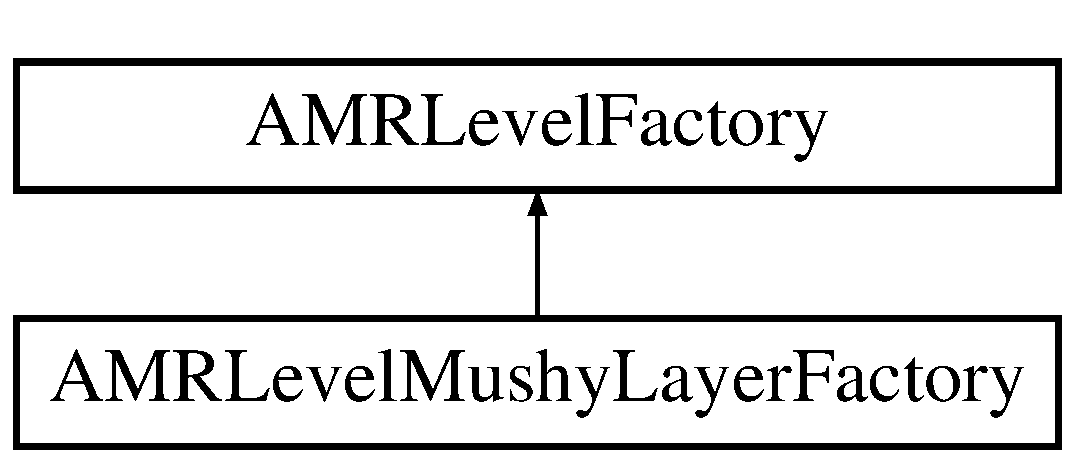
\includegraphics[height=2.000000cm]{class_a_m_r_level_mushy_layer_factory}
\end{center}
\end{figure}
\subsection*{Public Member Functions}
\begin{DoxyCompactItemize}
\item 
\hyperlink{class_a_m_r_level_mushy_layer_factory_af5500c64b1b300e8c11211aa617ff792}{A\-M\-R\-Level\-Mushy\-Layer\-Factory} (const Real \&a\-\_\-cfl, const Real \&a\-\_\-domain\-Width, const Real \&a\-\_\-refine\-Thresh, const int \&a\-\_\-tag\-Buffer\-Size, const bool \&a\-\_\-use\-Limiting)
\begin{DoxyCompactList}\small\item\em Constructor. \end{DoxyCompactList}\item 
\hypertarget{class_a_m_r_level_mushy_layer_factory_af574fd628470ed342ad0687f055924f1}{virtual \hyperlink{class_a_m_r_level_mushy_layer_factory_af574fd628470ed342ad0687f055924f1}{$\sim$\-A\-M\-R\-Level\-Mushy\-Layer\-Factory} ()}\label{class_a_m_r_level_mushy_layer_factory_af574fd628470ed342ad0687f055924f1}

\begin{DoxyCompactList}\small\item\em Destructor. \end{DoxyCompactList}\item 
\hypertarget{class_a_m_r_level_mushy_layer_factory_abf0a09d3816249031b1d583b74120355}{virtual A\-M\-R\-Level $\ast$ \hyperlink{class_a_m_r_level_mushy_layer_factory_abf0a09d3816249031b1d583b74120355}{new\-\_\-amrlevel} () const }\label{class_a_m_r_level_mushy_layer_factory_abf0a09d3816249031b1d583b74120355}

\begin{DoxyCompactList}\small\item\em Create new A\-M\-R\-Level. \end{DoxyCompactList}\end{DoxyCompactItemize}
\subsection*{Protected Attributes}
\begin{DoxyCompactItemize}
\item 
\hypertarget{class_a_m_r_level_mushy_layer_factory_a5ba6c44beb706a74802158e7490ac25b}{Real \hyperlink{class_a_m_r_level_mushy_layer_factory_a5ba6c44beb706a74802158e7490ac25b}{m\-\_\-cfl}}\label{class_a_m_r_level_mushy_layer_factory_a5ba6c44beb706a74802158e7490ac25b}

\begin{DoxyCompactList}\small\item\em C\-F\-L number. \end{DoxyCompactList}\item 
\hypertarget{class_a_m_r_level_mushy_layer_factory_adf85b7f5b35f914e1b31ad7aaeca5636}{Real \hyperlink{class_a_m_r_level_mushy_layer_factory_adf85b7f5b35f914e1b31ad7aaeca5636}{m\-\_\-domain\-Width}}\label{class_a_m_r_level_mushy_layer_factory_adf85b7f5b35f914e1b31ad7aaeca5636}

\begin{DoxyCompactList}\small\item\em Domain width. \end{DoxyCompactList}\item 
\hypertarget{class_a_m_r_level_mushy_layer_factory_ac2d21dd74453e56e44e1ddc52ff25afd}{Real \hyperlink{class_a_m_r_level_mushy_layer_factory_ac2d21dd74453e56e44e1ddc52ff25afd}{m\-\_\-refine\-Thresh}}\label{class_a_m_r_level_mushy_layer_factory_ac2d21dd74453e56e44e1ddc52ff25afd}

\begin{DoxyCompactList}\small\item\em Refinement threshold. \end{DoxyCompactList}\item 
\hypertarget{class_a_m_r_level_mushy_layer_factory_aa40e49179557fe927f578e5b4881790e}{int \hyperlink{class_a_m_r_level_mushy_layer_factory_aa40e49179557fe927f578e5b4881790e}{m\-\_\-tag\-Buffer\-Size}}\label{class_a_m_r_level_mushy_layer_factory_aa40e49179557fe927f578e5b4881790e}

\begin{DoxyCompactList}\small\item\em Tag buffer size. \end{DoxyCompactList}\item 
\hypertarget{class_a_m_r_level_mushy_layer_factory_a455170bf5a891c45e7647ca9f21af33a}{bool \hyperlink{class_a_m_r_level_mushy_layer_factory_a455170bf5a891c45e7647ca9f21af33a}{m\-\_\-use\-Limiting}}\label{class_a_m_r_level_mushy_layer_factory_a455170bf5a891c45e7647ca9f21af33a}

\begin{DoxyCompactList}\small\item\em Use slope limiting in advection calculations? \end{DoxyCompactList}\end{DoxyCompactItemize}


\subsection{Detailed Description}
Factory to create \hyperlink{class_a_m_r_level_mushy_layer}{A\-M\-R\-Level\-Mushy\-Layer}. 

Factory to create \hyperlink{class_a_m_r_level_mushy_layer}{A\-M\-R\-Level\-Mushy\-Layer} 

\subsection{Constructor \& Destructor Documentation}
\hypertarget{class_a_m_r_level_mushy_layer_factory_af5500c64b1b300e8c11211aa617ff792}{\index{A\-M\-R\-Level\-Mushy\-Layer\-Factory@{A\-M\-R\-Level\-Mushy\-Layer\-Factory}!A\-M\-R\-Level\-Mushy\-Layer\-Factory@{A\-M\-R\-Level\-Mushy\-Layer\-Factory}}
\index{A\-M\-R\-Level\-Mushy\-Layer\-Factory@{A\-M\-R\-Level\-Mushy\-Layer\-Factory}!AMRLevelMushyLayerFactory@{A\-M\-R\-Level\-Mushy\-Layer\-Factory}}
\subsubsection[{A\-M\-R\-Level\-Mushy\-Layer\-Factory}]{\setlength{\rightskip}{0pt plus 5cm}A\-M\-R\-Level\-Mushy\-Layer\-Factory\-::\-A\-M\-R\-Level\-Mushy\-Layer\-Factory (
\begin{DoxyParamCaption}
\item[{const Real \&}]{a\-\_\-cfl, }
\item[{const Real \&}]{a\-\_\-domain\-Width, }
\item[{const Real \&}]{a\-\_\-refine\-Thresh, }
\item[{const int \&}]{a\-\_\-tag\-Buffer\-Size, }
\item[{const bool \&}]{a\-\_\-use\-Limiting}
\end{DoxyParamCaption}
)}}\label{class_a_m_r_level_mushy_layer_factory_af5500c64b1b300e8c11211aa617ff792}


Constructor. 


\begin{DoxyParams}{Parameters}
{\em a\-\_\-cfl} & C\-F\-L number \\
\hline
{\em a\-\_\-domain\-Width} & physical width of domain \\
\hline
{\em a\-\_\-refine\-Thresh} & undivided gradient size over which a cell will be tagged for refinement \\
\hline
{\em a\-\_\-tag\-Buffer\-Size} & number of buffer cells around each tagged cell that will also be tagged \\
\hline
{\em a\-\_\-use\-Limiting} & whether to use van Leer limiting \\
\hline
\end{DoxyParams}


The documentation for this class was generated from the following files\-:\begin{DoxyCompactItemize}
\item 
/home/parkinsonjl/mushy-\/layer/src\-Subcycle/A\-M\-R\-Level\-Mushy\-Layer\-Factory.\-H\item 
/home/parkinsonjl/mushy-\/layer/src\-Subcycle/A\-M\-R\-Level\-Mushy\-Layer\-Factory.\-cpp\end{DoxyCompactItemize}

\hypertarget{classamr_mushy_layer}{\section{amr\-Mushy\-Layer Class Reference}
\label{classamr_mushy_layer}\index{amr\-Mushy\-Layer@{amr\-Mushy\-Layer}}
}


class to manage non-\/subcycled A\-M\-R computation of mushy layer dynamics  




{\ttfamily \#include $<$amr\-Mushy\-Layer.\-H$>$}

\subsection*{Public Member Functions}
\begin{DoxyCompactItemize}
\item 
\hyperlink{classamr_mushy_layer_a24060c00c555f171a510316e485e717a}{amr\-Mushy\-Layer} ()
\begin{DoxyCompactList}\small\item\em Default constructor. \end{DoxyCompactList}\item 
\hyperlink{classamr_mushy_layer_af0ccf706c8d1181abd8dd76fc4c51486}{$\sim$amr\-Mushy\-Layer} ()
\begin{DoxyCompactList}\small\item\em destructor \end{DoxyCompactList}\item 
\hypertarget{classamr_mushy_layer_a05a7ecf7f66e663d8fb68de84e6a5fc5}{void \hyperlink{classamr_mushy_layer_a05a7ecf7f66e663d8fb68de84e6a5fc5}{set\-Defaults} ()}\label{classamr_mushy_layer_a05a7ecf7f66e663d8fb68de84e6a5fc5}

\begin{DoxyCompactList}\small\item\em set default values before initialization \end{DoxyCompactList}\item 
void \hyperlink{classamr_mushy_layer_ac1e6c05047b20f43c849ffb5e409563e}{initialize} ()
\begin{DoxyCompactList}\small\item\em initializes object based on inputs data passed in through parm\-Parse \end{DoxyCompactList}\item 
\hypertarget{classamr_mushy_layer_ad3348089d05d4c0d90a9dbbfc2d62cd4}{void \hyperlink{classamr_mushy_layer_ad3348089d05d4c0d90a9dbbfc2d62cd4}{run} (Real a\-\_\-max\-\_\-time, int a\-\_\-max\-\_\-step)}\label{classamr_mushy_layer_ad3348089d05d4c0d90a9dbbfc2d62cd4}

\begin{DoxyCompactList}\small\item\em advance solution until either max\-\_\-time or max\-\_\-step are reached \end{DoxyCompactList}\item 
\hypertarget{classamr_mushy_layer_a2e73f3e60e9bbc8741a7d2be51a3dbb5}{bool \hyperlink{classamr_mushy_layer_a2e73f3e60e9bbc8741a7d2be51a3dbb5}{is\-Defined} () const }\label{classamr_mushy_layer_a2e73f3e60e9bbc8741a7d2be51a3dbb5}

\begin{DoxyCompactList}\small\item\em is this object defined and initialized? \end{DoxyCompactList}\end{DoxyCompactItemize}
\subsection*{Protected Types}
\begin{DoxyCompactItemize}
\item 
enum \hyperlink{classamr_mushy_layer_a0cf5dc1675842f2dcb139ba40f1f0ba0}{vector\-Vars} \{ \\*
{\bfseries m\-\_\-fluid\-Vel}, 
{\bfseries m\-\_\-fluid\-Vel\-Pred}, 
{\bfseries m\-\_\-grad\-Pressure}, 
{\bfseries m\-\_\-fluid\-Vel\-Analytic}, 
\\*
{\bfseries m\-\_\-fluid\-Vel\-Err}, 
{\bfseries m\-\_\-grad\-Pressure\-Err}
 \}
\begin{DoxyCompactList}\small\item\em List of vector fields. \end{DoxyCompactList}\item 
enum \hyperlink{classamr_mushy_layer_af138d45c7c0bf1d7e7efe38f7de2da96}{vars} \{ \\*
{\bfseries m\-\_\-enthalpy}, 
{\bfseries m\-\_\-enthalpy\-Solid}, 
{\bfseries m\-\_\-enthalpy\-Eutectic}, 
{\bfseries m\-\_\-enthalpy\-Liquid}, 
\\*
{\bfseries m\-\_\-composition}, 
{\bfseries m\-\_\-theta}, 
{\bfseries m\-\_\-theta\-Liquidus}, 
{\bfseries m\-\_\-theta\-Solidus}, 
\\*
{\bfseries m\-\_\-porosity}, 
{\bfseries m\-\_\-porosity\-Eutectic}, 
{\bfseries m\-\_\-composition\-Liquid}, 
{\bfseries m\-\_\-composition\-Solid}, 
\\*
{\bfseries m\-\_\-theta\-Forcing}, 
{\bfseries m\-\_\-liquid\-Composition\-Grad}, 
{\bfseries m\-\_\-solid\-Fraction}, 
{\bfseries m\-\_\-steady\-State\-Imbalance}, 
\\*
{\bfseries m\-\_\-\-Tanalytic}, 
{\bfseries m\-\_\-\-Theta\-L\-Analytic}, 
{\bfseries m\-\_\-solid\-Fraction\-True}, 
{\bfseries m\-\_\-theta\-True}, 
\\*
{\bfseries m\-\_\-\-Theta\-Analytic}, 
{\bfseries m\-\_\-enthalpy\-Analytic}, 
{\bfseries m\-\_\-enthalpy\-Advection}, 
{\bfseries m\-\_\-theta\-Laplacian}, 
\\*
{\bfseries m\-\_\-stream\-Function}, 
{\bfseries m\-\_\-resid}, 
{\bfseries m\-\_\-conc\-Source}, 
{\bfseries m\-\_\-\-Theta\-Diffusion}, 
\\*
{\bfseries m\-\_\-\-Theta\-Diffusion\-N}, 
{\bfseries m\-\_\-theta\-Bcoef}, 
{\bfseries m\-\_\-\-Theta\-B\-Coef}, 
{\bfseries m\-\_\-permeability}, 
\\*
{\bfseries m\-\_\-pressure}, 
{\bfseries m\-\_\-div\-U}, 
{\bfseries m\-\_\-\-Theta\-Frame\-Advection}, 
{\bfseries m\-\_\-\-Theta\-S\-Source}, 
\\*
{\bfseries m\-\_\-\-Theta\-Porosity\-Source}, 
{\bfseries m\-\_\-pressure\-Error}, 
{\bfseries m\-\_\-pressure\-Analytic}, 
{\bfseries m\-\_\-div\-Uerror}, 
\\*
{\bfseries m\-\_\-theta\-Forcing\-Error}, 
{\bfseries m\-\_\-theta\-Forcing\-Analytic}, 
{\bfseries m\-\_\-\-C\-F\-Interp\-Test}, 
{\bfseries m\-\_\-div\-Ustar}, 
\\*
{\bfseries m\-\_\-div\-Ustar\-Err}, 
{\bfseries m\-\_\-lambda}, 
{\bfseries m\-\_\-lambda\-Post\-Corr}, 
{\bfseries m\-\_\-buoyancy\-Filter}
 \}
\begin{DoxyCompactList}\small\item\em List of scalar fields. \end{DoxyCompactList}\item 
enum \hyperlink{classamr_mushy_layer_aa2979f33ff164690d99ca7f334c49ac7}{problem\-Type} \{ \\*
{\bfseries m\-\_\-full\-Problem}, 
{\bfseries m\-\_\-bm\-Diffusive\-Solidification}, 
{\bfseries m\-\_\-bm\-H\-R\-L}, 
{\bfseries m\-\_\-bm\-Diffusion}, 
\\*
{\bfseries m\-\_\-bm\-Advection}, 
{\bfseries m\-\_\-enforced\-Porosity}
 \}
\begin{DoxyCompactList}\small\item\em Which problem to solve? \end{DoxyCompactList}\item 
enum \hyperlink{classamr_mushy_layer_abd7c190080fa5c06b3587aae34a2af94}{frame\-Advection\-Methods} \{ {\bfseries m\-\_\-godunov}, 
{\bfseries m\-\_\-finite\-Difference}
 \}
\begin{DoxyCompactList}\small\item\em Different ways of calculating the frame advection term. \end{DoxyCompactList}\item 
enum \hyperlink{classamr_mushy_layer_a9ff26f4fd929196eb797c70e9a27d0d5}{domain\-Regions} \{ {\bfseries m\-\_\-solid\-Region}, 
{\bfseries m\-\_\-eutectic\-Region}, 
{\bfseries m\-\_\-mushy\-Region}, 
{\bfseries m\-\_\-liquid\-Region}
 \}
\begin{DoxyCompactList}\small\item\em Different phases we could be in. \end{DoxyCompactList}\end{DoxyCompactItemize}
\subsection*{Protected Member Functions}
\begin{DoxyCompactItemize}
\item 
void \hyperlink{classamr_mushy_layer_abf8a2ced1a62c3bf413494827c043a5d}{time\-Step} ()
\begin{DoxyCompactList}\small\item\em compute one timestep \end{DoxyCompactList}\item 
\hypertarget{classamr_mushy_layer_a84651402cfdf12a589571326ba3d76b0}{void \hyperlink{classamr_mushy_layer_a84651402cfdf12a589571326ba3d76b0}{regrid} ()}\label{classamr_mushy_layer_a84651402cfdf12a589571326ba3d76b0}

\begin{DoxyCompactList}\small\item\em do regridding \end{DoxyCompactList}\item 
\hypertarget{classamr_mushy_layer_ab4506f0846d5f996510308bac8bbc988}{void \hyperlink{classamr_mushy_layer_ab4506f0846d5f996510308bac8bbc988}{tag\-Cells} (Vector$<$ Int\-Vect\-Set $>$ \&a\-\_\-tags)}\label{classamr_mushy_layer_ab4506f0846d5f996510308bac8bbc988}

\begin{DoxyCompactList}\small\item\em compute tags for regridding \end{DoxyCompactList}\item 
\hypertarget{classamr_mushy_layer_a58f515311979c3fbb70d173c9a41b2b1}{void \hyperlink{classamr_mushy_layer_a58f515311979c3fbb70d173c9a41b2b1}{tag\-Cells\-Level} (Int\-Vect\-Set \&a\-\_\-tags, int a\-\_\-level)}\label{classamr_mushy_layer_a58f515311979c3fbb70d173c9a41b2b1}

\begin{DoxyCompactList}\small\item\em compute tags for the level a\-\_\-level \end{DoxyCompactList}\item 
\hypertarget{classamr_mushy_layer_addb6e9526d99bb162454080ebbc68c32}{void \hyperlink{classamr_mushy_layer_addb6e9526d99bb162454080ebbc68c32}{tag\-Cells\-Init} (Vector$<$ Int\-Vect\-Set $>$ \&a\-\_\-tags)}\label{classamr_mushy_layer_addb6e9526d99bb162454080ebbc68c32}

\begin{DoxyCompactList}\small\item\em compute tags at initial time \end{DoxyCompactList}\item 
\hypertarget{classamr_mushy_layer_a1596613735e6de7faa78dcc327267336}{void \hyperlink{classamr_mushy_layer_a1596613735e6de7faa78dcc327267336}{init\-Vars} (const int lev)}\label{classamr_mushy_layer_a1596613735e6de7faa78dcc327267336}

\begin{DoxyCompactList}\small\item\em Initialize all global variables on this level. \end{DoxyCompactList}\item 
\hypertarget{classamr_mushy_layer_aa29676c4f3489936cc67ee1fefcfc6fa}{void \hyperlink{classamr_mushy_layer_aa29676c4f3489936cc67ee1fefcfc6fa}{init\-Grids} (int a\-\_\-finest\-\_\-level)}\label{classamr_mushy_layer_aa29676c4f3489936cc67ee1fefcfc6fa}

\begin{DoxyCompactList}\small\item\em initialize grids at initial time \end{DoxyCompactList}\item 
\hypertarget{classamr_mushy_layer_ae4714d7bd538ceef23aae93667272158}{void \hyperlink{classamr_mushy_layer_ae4714d7bd538ceef23aae93667272158}{setup\-Fixed\-Grids} (const std\-::string \&a\-\_\-grid\-File)}\label{classamr_mushy_layer_ae4714d7bd538ceef23aae93667272158}

\begin{DoxyCompactList}\small\item\em set up grids from grids file \end{DoxyCompactList}\item 
\hypertarget{classamr_mushy_layer_a651b87329473d360eeaf90569d08e28e}{void \hyperlink{classamr_mushy_layer_a651b87329473d360eeaf90569d08e28e}{init\-Data} ()}\label{classamr_mushy_layer_a651b87329473d360eeaf90569d08e28e}

\begin{DoxyCompactList}\small\item\em initialize data on hierarchy \end{DoxyCompactList}\item 
\hypertarget{classamr_mushy_layer_a89fcf5b782c5325e9fe8ad9ed879dc3d}{void \hyperlink{classamr_mushy_layer_a89fcf5b782c5325e9fe8ad9ed879dc3d}{load\-From\-File} (const int a\-\_\-var, const string filename, const int num\-\_\-ghost, const int comp=0)}\label{classamr_mushy_layer_a89fcf5b782c5325e9fe8ad9ed879dc3d}

\begin{DoxyCompactList}\small\item\em Fill variable with data from file. \end{DoxyCompactList}\item 
\hypertarget{classamr_mushy_layer_a18162ee9e4bea27bf1e2d2c21cba7ac1}{Real \hyperlink{classamr_mushy_layer_a18162ee9e4bea27bf1e2d2c21cba7ac1}{time\-Dep\-Porosity} (Real x, Real z, Real t)}\label{classamr_mushy_layer_a18162ee9e4bea27bf1e2d2c21cba7ac1}

\begin{DoxyCompactList}\small\item\em Calculate time dependent porosity (for some benchmarks) \end{DoxyCompactList}\item 
\hypertarget{classamr_mushy_layer_a2992090df1afaa67bc95b148716df929}{void \hyperlink{classamr_mushy_layer_a2992090df1afaa67bc95b148716df929}{compute\-Dt} ()}\label{classamr_mushy_layer_a2992090df1afaa67bc95b148716df929}

\begin{DoxyCompactList}\small\item\em compute timestep \end{DoxyCompactList}\item 
\hypertarget{classamr_mushy_layer_a8573d490c20d6f6c2e069fee72dd81b8}{void \hyperlink{classamr_mushy_layer_a8573d490c20d6f6c2e069fee72dd81b8}{compute\-Initial\-Dt} ()}\label{classamr_mushy_layer_a8573d490c20d6f6c2e069fee72dd81b8}

\begin{DoxyCompactList}\small\item\em compute timestep at initial time \end{DoxyCompactList}\item 
\hypertarget{classamr_mushy_layer_afb9fd56d615299eb57fa799c58113d3a}{void \hyperlink{classamr_mushy_layer_afb9fd56d615299eb57fa799c58113d3a}{converged\-To\-Steady\-State} ()}\label{classamr_mushy_layer_afb9fd56d615299eb57fa799c58113d3a}

\begin{DoxyCompactList}\small\item\em Check if we've reached steady state. \end{DoxyCompactList}\item 
\hypertarget{classamr_mushy_layer_a547493d383066ed91739f7132b8d0715}{void \hyperlink{classamr_mushy_layer_a547493d383066ed91739f7132b8d0715}{setup\-Poisson\-Solvers} (Vector$<$ Level\-Data$<$ F\-Array\-Box $>$ $\ast$ $>$ \&a\-\_\-theta\-New, Vector$<$ Level\-Data$<$ F\-Array\-Box $>$ $\ast$ $>$ \&theta\-Source, Vector$<$ Level\-Data$<$ F\-Array\-Box $>$ $\ast$ $>$ \&a\-\_\-\-Theta\-L\-New, Vector$<$ Level\-Data$<$ F\-Array\-Box $>$ $\ast$ $>$ \&Theta\-Source, Vector$<$ Disjoint\-Box\-Layout $>$ \&active\-Grids)}\label{classamr_mushy_layer_a547493d383066ed91739f7132b8d0715}

\begin{DoxyCompactList}\small\item\em Initialise elliptic operators for $ \theta, \Theta_l $. \end{DoxyCompactList}\item 
\hypertarget{classamr_mushy_layer_a028dcc5f3cd2e10ebc5367d028e53d92}{void \hyperlink{classamr_mushy_layer_a028dcc5f3cd2e10ebc5367d028e53d92}{setup\-Multigrid} (Vector$<$ Level\-Data$<$ F\-Array\-Box $>$ $\ast$ $>$ \&a\-\_\-theta\-New, Vector$<$ Level\-Data$<$ F\-Array\-Box $>$ $\ast$ $>$ \&theta\-Source, Vector$<$ Level\-Data$<$ F\-Array\-Box $>$ $\ast$ $>$ \&a\-\_\-\-Theta\-L\-New, Vector$<$ Level\-Data$<$ F\-Array\-Box $>$ $\ast$ $>$ \&Theta\-L\-Source, Vector$<$ Disjoint\-Box\-Layout $>$ \&active\-Grids)}\label{classamr_mushy_layer_a028dcc5f3cd2e10ebc5367d028e53d92}

\begin{DoxyCompactList}\small\item\em Setup multigrid solvers and timestepping (backward euler, T\-G\-A etc.) \end{DoxyCompactList}\item 
\hypertarget{classamr_mushy_layer_a335bb9a21350557b2df0ee5213ab1a30}{void \hyperlink{classamr_mushy_layer_a335bb9a21350557b2df0ee5213ab1a30}{setup\-Advection\-Solvers} ()}\label{classamr_mushy_layer_a335bb9a21350557b2df0ee5213ab1a30}

\begin{DoxyCompactList}\small\item\em Initialise Godunov operators for frame advection calculations (enthalpy and bulk concentration) \end{DoxyCompactList}\item 
\hypertarget{classamr_mushy_layer_a26a96dc51faf448641df859c35f672f7}{void \hyperlink{classamr_mushy_layer_a26a96dc51faf448641df859c35f672f7}{setup\-I\-B\-C\-S} ()}\label{classamr_mushy_layer_a26a96dc51faf448641df859c35f672f7}

\begin{DoxyCompactList}\small\item\em Initialise various initial and boundary conditions. \end{DoxyCompactList}\item 
void \hyperlink{classamr_mushy_layer_a2f60c4520ecd9955f4fa9d26790b82d5}{get\-Active\-Grids\-Vars} (Vector$<$ Vector$<$ Ref\-Counted\-Ptr$<$ Level\-Data$<$ F\-Array\-Box $>$ $>$ $>$ $>$ \&a\-\_\-scalar\-New, Vector$<$ Vector$<$ Ref\-Counted\-Ptr$<$ Level\-Data$<$ F\-Array\-Box $>$ $>$ $>$ $>$ \&a\-\_\-scalar\-Old, Vector$<$ Disjoint\-Box\-Layout $>$ \&a\-\_\-amr\-Grids)
\item 
\hypertarget{classamr_mushy_layer_a402fc66363b84c6a064ef92ee8b37a1e}{void \hyperlink{classamr_mushy_layer_a402fc66363b84c6a064ef92ee8b37a1e}{get\-Level\-Advections\-Vars} (const int a\-\_\-var, const int lev, int \&ref\-Ratio, const bool has\-Coarser, const bool has\-Finer, const bool use\-\_\-limiting, Ref\-Counted\-Ptr$<$ Level\-Data$<$ F\-Array\-Box $>$ $>$ \&coarser\-Data\-Old\-Ptr\-Enthalpy, Ref\-Counted\-Ptr$<$ Level\-Data$<$ F\-Array\-Box $>$ $>$ \&coarser\-Data\-New\-Ptr\-Enthalpy, Ref\-Counted\-Ptr$<$ Level\-Flux\-Register $>$ \&coarser\-F\-R\-Ptr\-Enthalpy, Ref\-Counted\-Ptr$<$ Level\-Flux\-Register $>$ \&finer\-F\-R\-Ptr\-Enthalpy, Disjoint\-Box\-Layout \&coarse\-Grid, \hyperlink{class_level_advect}{Level\-Advect} \&lev\-Advect, Real \&t\-Coarser\-New, Real \&t\-Coarser\-Old)}\label{classamr_mushy_layer_a402fc66363b84c6a064ef92ee8b37a1e}

\begin{DoxyCompactList}\small\item\em Get all the variables needed to calculate advection on this level. \end{DoxyCompactList}\item 
void \hyperlink{classamr_mushy_layer_a6ba0c9d6199a5aed7ad596639c90656d}{get\-Frame\-Advection} (const int lev)
\item 
\hypertarget{classamr_mushy_layer_af3003a8b8122c744d6809731b1940210}{void \hyperlink{classamr_mushy_layer_af3003a8b8122c744d6809731b1940210}{get\-Fluid\-Advection} (const int lev)}\label{classamr_mushy_layer_af3003a8b8122c744d6809731b1940210}

\begin{DoxyCompactList}\small\item\em Convert the F\-Array\-Box of fluid velocities to a fluxbox. \end{DoxyCompactList}\item 
void \hyperlink{classamr_mushy_layer_ad1f6a703a258aa8a10185fcd72a6d988}{theta\-V\-C\-Op\-Coeffs} (Real \&alpha, Real \&beta, Vector$<$ Ref\-Counted\-Ptr$<$ Level\-Data$<$ F\-Array\-Box $>$ $>$ $>$ \&a\-Coef, Vector$<$ Ref\-Counted\-Ptr$<$ Level\-Data$<$ Flux\-Box $>$ $>$ $>$ \&b\-Coef)
\begin{DoxyCompactList}\small\item\em Get coefficients for the $ \theta $ V\-C\-A\-M\-R\-Poisson\-Op2 object. \end{DoxyCompactList}\item 
void \hyperlink{classamr_mushy_layer_aac3e8f11df8de976c0be9ab054a76e6b}{advect\-Scalar} (int a\-\_\-var, Vector$<$ Level\-Data$<$ F\-Array\-Box $>$ $\ast$ $>$ a\-\_\-source, Vector$<$ Level\-Data$<$ Flux\-Box $>$ $\ast$ $>$ a\-\_\-adv\-Vel)
\item 
\hypertarget{classamr_mushy_layer_a734cdc2ecc10363633bd1b6d4651dbb0}{void \hyperlink{classamr_mushy_layer_a734cdc2ecc10363633bd1b6d4651dbb0}{do\-Reflux} (int a\-\_\-var, int reflux\-Level)}\label{classamr_mushy_layer_a734cdc2ecc10363633bd1b6d4651dbb0}

\begin{DoxyCompactList}\small\item\em reflux \end{DoxyCompactList}\item 
\hypertarget{classamr_mushy_layer_a15862a52a9c7ef32d940d471260e79cb}{void \hyperlink{classamr_mushy_layer_a15862a52a9c7ef32d940d471260e79cb}{do\-Implicit\-Reflux} (int a\-\_\-var, int lev)}\label{classamr_mushy_layer_a15862a52a9c7ef32d940d471260e79cb}

\begin{DoxyCompactList}\small\item\em Reflux for when we have diffusion as well. Ripped from A\-M\-R\-Godunov example. \end{DoxyCompactList}\item 
\hypertarget{classamr_mushy_layer_aff391cf87d3082ffd28ba1ec6d10ece6}{void \hyperlink{classamr_mushy_layer_aff391cf87d3082ffd28ba1ec6d10ece6}{make\-Advection\-Term} (const int a\-\_\-var, const Vector$<$ Level\-Data$<$ F\-Array\-Box $>$ $\ast$ $>$ a\-\_\-source, const Vector$<$ Level\-Data$<$ Flux\-Box $>$ $\ast$ $>$ a\-\_\-adv\-Vel, Vector$<$ Ref\-Counted\-Ptr$<$ Level\-Data$<$ F\-Array\-Box $>$ $>$ $>$ a\-\_\-adv\-Term)}\label{classamr_mushy_layer_aff391cf87d3082ffd28ba1ec6d10ece6}

\begin{DoxyCompactList}\small\item\em Advect scalar and put U.\-grad(var) into a\-\_\-adv\-Term. \end{DoxyCompactList}\item 
\hypertarget{classamr_mushy_layer_ab217064d67f9cfb5f9b862f3f2700aeb}{void \hyperlink{classamr_mushy_layer_ab217064d67f9cfb5f9b862f3f2700aeb}{active\-Level\-Copy} (Vector$<$ Ref\-Counted\-Ptr$<$ Level\-Data$<$ F\-Array\-Box $>$ $>$ $>$ from, Vector$<$ Ref\-Counted\-Ptr$<$ Level\-Data$<$ F\-Array\-Box $>$ $>$ $>$ to)}\label{classamr_mushy_layer_ab217064d67f9cfb5f9b862f3f2700aeb}

\begin{DoxyCompactList}\small\item\em Copy across all the active levels of a Vector$<$\-Level\-Data$>$ to another. \end{DoxyCompactList}\item 
void \hyperlink{classamr_mushy_layer_accf7a2c238f97c60a3a4ad83b02add7e}{calculatetheta\-Source\-Term} (Vector$<$ Level\-Data$<$ F\-Array\-Box $>$ $\ast$ $>$ theta\-Source, Vector$<$ Level\-Data$<$ F\-Array\-Box $>$ $\ast$ $>$ V\-\_\-grad\-H)
\item 
\hypertarget{classamr_mushy_layer_a736acc5a72c3760580565312c8df1547}{void \hyperlink{classamr_mushy_layer_a736acc5a72c3760580565312c8df1547}{calculate\-Enthalpy} ()}\label{classamr_mushy_layer_a736acc5a72c3760580565312c8df1547}

\begin{DoxyCompactList}\small\item\em Calculate $ H = \chi S + (\chi + (1-\chi) c_p)\theta $. \end{DoxyCompactList}\item 
\hypertarget{classamr_mushy_layer_ac2ce75e559b336ca9fa9c2c72c224249}{void \hyperlink{classamr_mushy_layer_ac2ce75e559b336ca9fa9c2c72c224249}{calculate\-Bulk\-Concentration} ()}\label{classamr_mushy_layer_ac2ce75e559b336ca9fa9c2c72c224249}

\begin{DoxyCompactList}\small\item\em Calculate $ \Theta = \chi \Theta_l + (1-\chi) \Theta_s$. \end{DoxyCompactList}\item 
\hypertarget{classamr_mushy_layer_ac2534289ebb1a6150257076e00a89d75}{void \hyperlink{classamr_mushy_layer_ac2534289ebb1a6150257076e00a89d75}{calculate\-Porosity} ()}\label{classamr_mushy_layer_ac2534289ebb1a6150257076e00a89d75}

\begin{DoxyCompactList}\small\item\em Calculate porosity using the phase diagram. \end{DoxyCompactList}\item 
\hypertarget{classamr_mushy_layer_a4e5595ecd8886f14a9e585aaca80f13f}{void \hyperlink{classamr_mushy_layer_a4e5595ecd8886f14a9e585aaca80f13f}{make\-Laplacian} (const int a\-\_\-var, const int lev, Level\-Data$<$ F\-Array\-Box $>$ \&a\-\_\-laplacian)}\label{classamr_mushy_layer_a4e5595ecd8886f14a9e585aaca80f13f}

\begin{DoxyCompactList}\small\item\em Calculate $ \nabla^2 \phi $ on this level if we have an operator for that. \end{DoxyCompactList}\item 
\hypertarget{classamr_mushy_layer_af2ae32e36e6ea4f55e82d4ae02f44374}{void \hyperlink{classamr_mushy_layer_af2ae32e36e6ea4f55e82d4ae02f44374}{update\-Enthalpy\-Variables} ()}\label{classamr_mushy_layer_af2ae32e36e6ea4f55e82d4ae02f44374}

\begin{DoxyCompactList}\small\item\em Update enthalpy method variables. \end{DoxyCompactList}\item 
\hypertarget{classamr_mushy_layer_acad764d7b02e9d3a46aecd5fa9291658}{Real \hyperlink{classamr_mushy_layer_acad764d7b02e9d3a46aecd5fa9291658}{calculate\-Heat\-Eqn\-Residual2} (const Vector$<$ Level\-Data$<$ F\-Array\-Box $>$ $\ast$ $>$a\-\_\-theta\-New, const Vector$<$ Level\-Data$<$ F\-Array\-Box $>$ $\ast$ $>$ a\-\_\-theta\-New\-Prev)}\label{classamr_mushy_layer_acad764d7b02e9d3a46aecd5fa9291658}

\begin{DoxyCompactList}\small\item\em Calculate $ H^{k} - H^{k+1} $ where $ k $ is the iteration number. \end{DoxyCompactList}\item 
\hypertarget{classamr_mushy_layer_a6ec9dce5f92315519275f8f77a90e968}{void \hyperlink{classamr_mushy_layer_a6ec9dce5f92315519275f8f77a90e968}{calculate\-Analytic\-Solution} ()}\label{classamr_mushy_layer_a6ec9dce5f92315519275f8f77a90e968}

\begin{DoxyCompactList}\small\item\em Calculate the analytic solution for this particular problem if possible. \end{DoxyCompactList}\item 
\hypertarget{classamr_mushy_layer_aec43865ff120106dd5b24076b0cc293e}{void \hyperlink{classamr_mushy_layer_aec43865ff120106dd5b24076b0cc293e}{calculate\-Soln\-Bm1} ()}\label{classamr_mushy_layer_aec43865ff120106dd5b24076b0cc293e}

\begin{DoxyCompactList}\small\item\em Analytic solution for benchmark 1 -\/ directional solidification without flow (Worster 1991) \end{DoxyCompactList}\item 
\hypertarget{classamr_mushy_layer_a2b24a38504f094c84f33481e81e3c5ac}{void \hyperlink{classamr_mushy_layer_a2b24a38504f094c84f33481e81e3c5ac}{calculate\-Soln\-Diffusion} ()}\label{classamr_mushy_layer_a2b24a38504f094c84f33481e81e3c5ac}

\begin{DoxyCompactList}\small\item\em Analytic solution for simple temperature diffusion $ \partial \theta / \partial t = \nabla^2 \theta $. \end{DoxyCompactList}\item 
\hypertarget{classamr_mushy_layer_a9c562e8758d467e0e917ae2fd5b35c3c}{void \hyperlink{classamr_mushy_layer_a9c562e8758d467e0e917ae2fd5b35c3c}{calculate\-Soln\-Bm2} ()}\label{classamr_mushy_layer_a9c562e8758d467e0e917ae2fd5b35c3c}

\begin{DoxyCompactList}\small\item\em Analytic solution for benchmark 2 -\/ flow in a fixed porous medium. \end{DoxyCompactList}\item 
\hypertarget{classamr_mushy_layer_a026ec617dc4f07424222aed6e1ada71e}{void \hyperlink{classamr_mushy_layer_a026ec617dc4f07424222aed6e1ada71e}{enforce\-Analytic\-Solution} ()}\label{classamr_mushy_layer_a026ec617dc4f07424222aed6e1ada71e}

\begin{DoxyCompactList}\small\item\em Fill the fields used in calculations with the analytic values, if possible. \end{DoxyCompactList}\item 
\hypertarget{classamr_mushy_layer_a72a4f6cf4f003bc955237811f5f17e05}{void \hyperlink{classamr_mushy_layer_a72a4f6cf4f003bc955237811f5f17e05}{write\-Solution\-To\-Text\-File} (int lev)}\label{classamr_mushy_layer_a72a4f6cf4f003bc955237811f5f17e05}

\begin{DoxyCompactList}\small\item\em Write the primary variables of the current solution to a text file. \end{DoxyCompactList}\item 
\hypertarget{classamr_mushy_layer_ad108111c89c43cb54a5d362fc3425a12}{void \hyperlink{classamr_mushy_layer_ad108111c89c43cb54a5d362fc3425a12}{average\-Coarse\-To\-Fine\-Solutions} ()}\label{classamr_mushy_layer_ad108111c89c43cb54a5d362fc3425a12}

\begin{DoxyCompactList}\small\item\em replace coarse data with the average of finer data where appropriate \end{DoxyCompactList}\item 
\hypertarget{classamr_mushy_layer_a54969e4eb65f804525820e4f13ab09b2}{void \hyperlink{classamr_mushy_layer_a54969e4eb65f804525820e4f13ab09b2}{interp\-To\-Fine\-Solutions} (int lev, const std\-::vector$<$ int $>$ scalar\-Vars=std\-::vector$<$ int $>$(), const std\-::vector$<$ int $>$ \hyperlink{classamr_mushy_layer_a0cf5dc1675842f2dcb139ba40f1f0ba0}{vector\-Vars}=std\-::vector$<$ int $>$())}\label{classamr_mushy_layer_a54969e4eb65f804525820e4f13ab09b2}

\begin{DoxyCompactList}\small\item\em Fill fine levels with data from coarser levels. \end{DoxyCompactList}\item 
\hypertarget{classamr_mushy_layer_a91c301183cfb40d065cf15f332de0056}{bool \hyperlink{classamr_mushy_layer_a91c301183cfb40d065cf15f332de0056}{residuals\-Diverging} (const Vector$<$ Real $>$ residuals)}\label{classamr_mushy_layer_a91c301183cfb40d065cf15f332de0056}

\begin{DoxyCompactList}\small\item\em Check a sequence of residuals isn't diverging. \end{DoxyCompactList}\item 
\hypertarget{classamr_mushy_layer_a1ddc3d2211b8610021a1520039af8ef9}{bool \hyperlink{classamr_mushy_layer_a1ddc3d2211b8610021a1520039af8ef9}{residuals\-Constant} (const Vector$<$ Real $>$ residuals)}\label{classamr_mushy_layer_a1ddc3d2211b8610021a1520039af8ef9}

\begin{DoxyCompactList}\small\item\em Check that a sequence of residuals isn't equal (relative to our tolerance level) \end{DoxyCompactList}\item 
\hypertarget{classamr_mushy_layer_a6ee5e0d648d50df048b2ad4f1caffdde}{void \hyperlink{classamr_mushy_layer_a6ee5e0d648d50df048b2ad4f1caffdde}{setup\-Flux\-Registers} ()}\label{classamr_mushy_layer_a6ee5e0d648d50df048b2ad4f1caffdde}

\begin{DoxyCompactList}\small\item\em Set up flux registers. \end{DoxyCompactList}\item 
\hypertarget{classamr_mushy_layer_a2c10fd1cc77ccb14d4d4c5c2806548dd}{void \hyperlink{classamr_mushy_layer_a2c10fd1cc77ccb14d4d4c5c2806548dd}{do\-C\-F\-Interp\-Test} ()}\label{classamr_mushy_layer_a2c10fd1cc77ccb14d4d4c5c2806548dd}

\begin{DoxyCompactList}\small\item\em A test to see what C\-F interp does. \end{DoxyCompactList}\item 
\hypertarget{classamr_mushy_layer_a78d9b1fe087c0b66f2644a1edd708dcf}{void \hyperlink{classamr_mushy_layer_a78d9b1fe087c0b66f2644a1edd708dcf}{calculate\-Frame\-Advection} (int a\-\_\-var, Vector$<$ Level\-Data$<$ F\-Array\-Box $>$ $\ast$ $>$ \&a\-\_\-grad, Real frame\-Adv\-Vel)}\label{classamr_mushy_layer_a78d9b1fe087c0b66f2644a1edd708dcf}

\begin{DoxyCompactList}\small\item\em Calculate $ V d \phi / dt $ using a one sided, second order, finite difference. \end{DoxyCompactList}\item 
\hypertarget{classamr_mushy_layer_aadf951416861e7913d032f10e034f1fb}{void \hyperlink{classamr_mushy_layer_aadf951416861e7913d032f10e034f1fb}{calculate\-Frame\-Advection\-Godunov} (const int a\-\_\-var)}\label{classamr_mushy_layer_aadf951416861e7913d032f10e034f1fb}

\begin{DoxyCompactList}\small\item\em Calculate $ V d \phi / dt $ using a Godunov (flux conservative) method. Think this is first order in space. \end{DoxyCompactList}\item 
void \hyperlink{classamr_mushy_layer_a75ef657901ce964fd2ea6b0d92e9c65f}{calculate\-Theta\-L\-Source\-Term} (Vector$<$ Level\-Data$<$ F\-Array\-Box $>$ $\ast$ $>$ V\-\_\-d\-Thetadz\-\_\-n, Vector$<$ Level\-Data$<$ F\-Array\-Box $>$ $\ast$ $>$ Theta\-Diffusion\-\_\-n)
\item 
\hypertarget{classamr_mushy_layer_a3db516a1b0dc1b9e7aeaa17f47157c9c}{void \hyperlink{classamr_mushy_layer_a3db516a1b0dc1b9e7aeaa17f47157c9c}{calculate\-Theta\-Diffusion} (Vector$<$ Level\-Data$<$ F\-Array\-Box $>$ $\ast$ $>$ a\-\_\-\-Theta\-Diffusion)}\label{classamr_mushy_layer_a3db516a1b0dc1b9e7aeaa17f47157c9c}

\begin{DoxyCompactList}\small\item\em Calculate $ Le^{-1} \nabla \chi \nabla \Theta_l $. \end{DoxyCompactList}\item 
\hypertarget{classamr_mushy_layer_aa6d3cfa6c1b4bfa2938d9ccbc44f516e}{void \hyperlink{classamr_mushy_layer_aa6d3cfa6c1b4bfa2938d9ccbc44f516e}{calculatetheta\-Diffusion} (Vector$<$ Ref\-Counted\-Ptr$<$ Level\-Data$<$ F\-Array\-Box $>$ $>$ $>$ \&a\-\_\-\-Theta\-Diffusion, Vector$<$ Level\-Data$<$ F\-Array\-Box $>$ $\ast$ $>$ \&a\-\_\-theta\-Old)}\label{classamr_mushy_layer_aa6d3cfa6c1b4bfa2938d9ccbc44f516e}

\begin{DoxyCompactList}\small\item\em Calculate $ \nabla^2 \theta $. \end{DoxyCompactList}\item 
Real \hyperlink{classamr_mushy_layer_a97818cd2b7076805211c086af2d375f1}{calculate\-Residual2} (const Vector$<$ Ref\-Counted\-Ptr$<$ Level\-Data$<$ F\-Array\-Box $>$ $>$ $>$ a\-\_\-phi\-Old, const Vector$<$ Ref\-Counted\-Ptr$<$ Level\-Data$<$ F\-Array\-Box $>$ $>$ $>$ a\-\_\-phi\-New)
\item 
void \hyperlink{classamr_mushy_layer_a876a962765e746e053aed9f8383868a6}{update\-Velocity} (Vector$<$ Disjoint\-Box\-Layout $>$ active\-Grids, Real alpha=0)
\item 
\hypertarget{classamr_mushy_layer_a2497035467f060ad356e6f1c63c717c9}{void \hyperlink{classamr_mushy_layer_a2497035467f060ad356e6f1c63c717c9}{update\-Velocity\-Comp} (Vector$<$ Disjoint\-Box\-Layout $>$ active\-Grids, Real alpha=0)}\label{classamr_mushy_layer_a2497035467f060ad356e6f1c63c717c9}

\begin{DoxyCompactList}\small\item\em Not used anymore. \end{DoxyCompactList}\item 
\hypertarget{classamr_mushy_layer_a6fef0624f462d75984aca1c995f8c2aa}{void \hyperlink{classamr_mushy_layer_a6fef0624f462d75984aca1c995f8c2aa}{do\-Implicit\-Velocity\-Reflux} (int m\-\_\-level)}\label{classamr_mushy_layer_a6fef0624f462d75984aca1c995f8c2aa}

\begin{DoxyCompactList}\small\item\em Do implicity velocity reflux on level. \end{DoxyCompactList}\item 
\hypertarget{classamr_mushy_layer_a09ace24946676ed537647ccd6950bc5b}{void \hyperlink{classamr_mushy_layer_a09ace24946676ed537647ccd6950bc5b}{do\-Explicit\-Velocity\-Reflux} ()}\label{classamr_mushy_layer_a09ace24946676ed537647ccd6950bc5b}

\begin{DoxyCompactList}\small\item\em Do explicit velocity reflux. \end{DoxyCompactList}\item 
\hypertarget{classamr_mushy_layer_a28fe2843693ea38d7be472049f7eae28}{void \hyperlink{classamr_mushy_layer_a28fe2843693ea38d7be472049f7eae28}{init\-Scalar\-Vars} (const int lev)}\label{classamr_mushy_layer_a28fe2843693ea38d7be472049f7eae28}

\begin{DoxyCompactList}\small\item\em Initialise all scalar fields on this level, so the data structures can be used. \end{DoxyCompactList}\item 
\hypertarget{classamr_mushy_layer_a92d0abef37c6cdb9e3546624c96a6ac7}{void \hyperlink{classamr_mushy_layer_a92d0abef37c6cdb9e3546624c96a6ac7}{init\-Vector\-Vars} (const int lev)}\label{classamr_mushy_layer_a92d0abef37c6cdb9e3546624c96a6ac7}

\begin{DoxyCompactList}\small\item\em Initialise all vector fields on this level, so the data structures can be used. \end{DoxyCompactList}\item 
Vector$<$ Level\-Data$<$ F\-Array\-Box $>$ $\ast$ $>$ \hyperlink{classamr_mushy_layer_a7b11792039dd642fccc7af0e757408f4}{time\-Centered\-Scalar} (const int a\-\_\-var)
\item 
\hypertarget{classamr_mushy_layer_a927fa5b33122ac70bb19a9d65d0c4416}{void \hyperlink{classamr_mushy_layer_a927fa5b33122ac70bb19a9d65d0c4416}{enforce\-Abs\-Cap} (Vector$<$ Ref\-Counted\-Ptr$<$ Level\-Data$<$ F\-Array\-Box $>$ $>$ $>$ a\-\_\-phi, Real a\-\_\-cap)}\label{classamr_mushy_layer_a927fa5b33122ac70bb19a9d65d0c4416}

\begin{DoxyCompactList}\small\item\em For each value x in a\-\_\-phi, if $\vert$x$\vert$ $>$ $\vert$a\-\_\-cap$\vert$ set x=a\-\_\-cap (with the relevant sign) \end{DoxyCompactList}\item 
\hypertarget{classamr_mushy_layer_a627e21c7786688fc1723e738f6f3ce0e}{void \hyperlink{classamr_mushy_layer_a627e21c7786688fc1723e738f6f3ce0e}{remove\-Nan\-Values} (F\-Array\-Box \&fab)}\label{classamr_mushy_layer_a627e21c7786688fc1723e738f6f3ce0e}

\begin{DoxyCompactList}\small\item\em Remove nan values and replace them with 0. \end{DoxyCompactList}\item 
\hypertarget{classamr_mushy_layer_a4b534f6320075017ec12636e721ebf9a}{bool \hyperlink{classamr_mushy_layer_a4b534f6320075017ec12636e721ebf9a}{nonlinear\-Solver} (Vector$<$ Vector$<$ Ref\-Counted\-Ptr$<$ Level\-Data$<$ F\-Array\-Box $>$ $>$ $>$ $>$ a\-\_\-scalar\-New, Vector$<$ Vector$<$ Ref\-Counted\-Ptr$<$ Level\-Data$<$ F\-Array\-Box $>$ $>$ $>$ $>$a\-\_\-scalar\-Old, Vector$<$ Disjoint\-Box\-Layout $>$ a\-\_\-amr\-Grids, Vector$<$ Level\-Data$<$ F\-Array\-Box $>$ $\ast$ $>$ a\-\_\-theta\-New, Vector$<$ Level\-Data$<$ F\-Array\-Box $>$ $\ast$ $>$ a\-\_\-theta\-Old, Vector$<$ Level\-Data$<$ F\-Array\-Box $>$ $\ast$ $>$ a\-\_\-theta\-Diff, Vector$<$ Level\-Data$<$ F\-Array\-Box $>$ $\ast$ $>$ a\-\_\-theta\-Old\-Temp, Vector$<$ Level\-Data$<$ F\-Array\-Box $>$ $\ast$ $>$ a\-\_\-\-Theta\-L\-New, Vector$<$ Level\-Data$<$ F\-Array\-Box $>$ $\ast$ $>$ a\-\_\-\-Theta\-L\-Old, Vector$<$ Level\-Data$<$ F\-Array\-Box $>$ $\ast$ $>$ a\-\_\-theta\-New\-Prev, Vector$<$ Level\-Data$<$ F\-Array\-Box $>$ $\ast$ $>$ zero\-Source, Vector$<$ Level\-Data$<$ F\-Array\-Box $>$ $\ast$ $>$ V\-\_\-grad\-H\-\_\-n, Vector$<$ Level\-Data$<$ F\-Array\-Box $>$ $\ast$ $>$ V\-\_\-d\-Thetadz\-\_\-n, Vector$<$ Level\-Data$<$ F\-Array\-Box $>$ $\ast$ $>$ theta\-Source, Vector$<$ Level\-Data$<$ F\-Array\-Box $>$ $\ast$ $>$ Theta\-L\-Source, Vector$<$ Ref\-Counted\-Ptr$<$ Level\-Data$<$ F\-Array\-Box $>$ $>$ $>$ a\-\_\-\-Theta\-Prev\-Iteration, Vector$<$ Ref\-Counted\-Ptr$<$ Level\-Data$<$ F\-Array\-Box $>$ $>$ $>$ a\-\_\-\-H\-Prev\-Iteration, Vector$<$ Ref\-Counted\-Ptr$<$ Level\-Data$<$ F\-Array\-Box $>$ $>$ $>$ a\-\_\-\-Theta\-Two\-Prev, Vector$<$ Ref\-Counted\-Ptr$<$ Level\-Data$<$ F\-Array\-Box $>$ $>$ $>$ a\-\_\-\-H\-Two\-Prev, Real residual\-Enthalpy, Real residual\-Conc, Vector$<$ Real $>$ \&heat\-Residuals, Vector$<$ Real $>$ \&conc\-Residuals, int \&iteration)}\label{classamr_mushy_layer_a4b534f6320075017ec12636e721ebf9a}

\begin{DoxyCompactList}\small\item\em Do one iteration of the nonlinear solver. \end{DoxyCompactList}\item 
void \hyperlink{classamr_mushy_layer_adada677b759fd1b2e5236b9002e5990c}{get\-Theta\-L\-Op\-Coeffs} (Real \&alpha, Real \&beta, Vector$<$ Ref\-Counted\-Ptr$<$ Level\-Data$<$ F\-Array\-Box $>$ $>$ $>$ \&a\-Coef, Vector$<$ Ref\-Counted\-Ptr$<$ Level\-Data$<$ Flux\-Box $>$ $>$ $>$ \&b\-Coef)
\item 
\hypertarget{classamr_mushy_layer_a117c9ac8cf3066b5826d3cd15d98d84c}{void \hyperlink{classamr_mushy_layer_a117c9ac8cf3066b5826d3cd15d98d84c}{log\-Message} (int priority, string message)}\label{classamr_mushy_layer_a117c9ac8cf3066b5826d3cd15d98d84c}

\begin{DoxyCompactList}\small\item\em helper function -\/ if priority $>$= s\-\_\-verbosity, write out message \end{DoxyCompactList}\item 
\hypertarget{classamr_mushy_layer_aa01cbe0216c124b1f6731b52e79a0587}{void \hyperlink{classamr_mushy_layer_aa01cbe0216c124b1f6731b52e79a0587}{ptr\-To\-Ref\-Counted\-Ptr} (Vector$<$ Level\-Data$<$ F\-Array\-Box $>$ $\ast$ $>$ \&ptr, Vector$<$ Ref\-Counted\-Ptr$<$ Level\-Data$<$ F\-Array\-Box $>$ $>$ $>$ \&ref\-Ptr)}\label{classamr_mushy_layer_aa01cbe0216c124b1f6731b52e79a0587}

\begin{DoxyCompactList}\small\item\em Take a pointer and return a Ref\-Counted\-Ptr to the same data. \end{DoxyCompactList}\item 
\hypertarget{classamr_mushy_layer_a917e8918451988372e556e8f8f4e391c}{void \hyperlink{classamr_mushy_layer_a917e8918451988372e556e8f8f4e391c}{ref\-Counted\-Ptr\-To\-Ptr} (Vector$<$ Ref\-Counted\-Ptr$<$ Level\-Data$<$ F\-Array\-Box $>$ $>$ $>$ \&ref\-Ptr, Vector$<$ Level\-Data$<$ F\-Array\-Box $>$ $\ast$ $>$ \&ptr)}\label{classamr_mushy_layer_a917e8918451988372e556e8f8f4e391c}

\begin{DoxyCompactList}\small\item\em Take a Ref\-Counted\-Ptr and return a pointer to the same data. \end{DoxyCompactList}\item 
\hypertarget{classamr_mushy_layer_acbd65aadd4ec5c022282a9633d7a6959}{void \hyperlink{classamr_mushy_layer_acbd65aadd4ec5c022282a9633d7a6959}{get\-Location} (const Int\-Vect iv, const int lev, Real\-Vect \&loc, Real cc\-Offset\-X=0.\-5, Real cc\-Offset\-Y=0.\-5)}\label{classamr_mushy_layer_acbd65aadd4ec5c022282a9633d7a6959}

\begin{DoxyCompactList}\small\item\em Get the actual location (x,y,z) of an Int\-Vect. \end{DoxyCompactList}\item 
\hypertarget{classamr_mushy_layer_ab43481a5faeb81d3641d522599851384}{void \hyperlink{classamr_mushy_layer_ab43481a5faeb81d3641d522599851384}{get\-Var\-Names} (Vector$<$ string $>$ \&var\-Names)}\label{classamr_mushy_layer_ab43481a5faeb81d3641d522599851384}

\begin{DoxyCompactList}\small\item\em Get a vector containing all var names (scalar and vector components) \end{DoxyCompactList}\item 
void \hyperlink{classamr_mushy_layer_a94dadf602acc348aa6a00714fe5e3338}{get\-Pressure\-V\-Ccoefs} (Vector$<$ Ref\-Counted\-Ptr$<$ Level\-Data$<$ F\-Array\-Box $>$ $>$ $>$ \&a\-Coef, Vector$<$ Ref\-Counted\-Ptr$<$ Level\-Data$<$ Flux\-Box $>$ $>$ $>$ \&b\-Coef)
\item 
\hypertarget{classamr_mushy_layer_a1a941f38c0efa3626ff8bb49278c0e0a}{void \hyperlink{classamr_mushy_layer_a1a941f38c0efa3626ff8bb49278c0e0a}{apply\-B\-Cs} (const int a\-\_\-var, const int lev)}\label{classamr_mushy_layer_a1a941f38c0efa3626ff8bb49278c0e0a}

\begin{DoxyCompactList}\small\item\em apply boundary conditions to a specific variable (if possible) and on a specific level (if specified) \end{DoxyCompactList}\item 
\hypertarget{classamr_mushy_layer_ae00c39bc7eaf2a9203a6779426e27ede}{void \hyperlink{classamr_mushy_layer_ae00c39bc7eaf2a9203a6779426e27ede}{apply\-Vector\-B\-Cs} (const int a\-\_\-var, const int lev)}\label{classamr_mushy_layer_ae00c39bc7eaf2a9203a6779426e27ede}

\begin{DoxyCompactList}\small\item\em apply boundary conditions to vector field \end{DoxyCompactList}\item 
\hypertarget{classamr_mushy_layer_ae495b9a6e1b154a504d5ab31ac3e546a}{void \hyperlink{classamr_mushy_layer_ae495b9a6e1b154a504d5ab31ac3e546a}{apply\-B\-Cs} (int a\-\_\-var)}\label{classamr_mushy_layer_ae495b9a6e1b154a504d5ab31ac3e546a}

\begin{DoxyCompactList}\small\item\em apply boundary conditions to a specific variable (if possible) on all levels \end{DoxyCompactList}\item 
\hypertarget{classamr_mushy_layer_acf79957581036bb510de411d03fd8f10}{Real \hyperlink{classamr_mushy_layer_acf79957581036bb510de411d03fd8f10}{calculate\-Max\-Diff} (Vector$<$ Level\-Data$<$ F\-Array\-Box $>$ $\ast$ $>$ a\-\_\-phi\-New, Vector$<$ Level\-Data$<$ F\-Array\-Box $>$ $\ast$ $>$ a\-\_\-phi\-Old)}\label{classamr_mushy_layer_acf79957581036bb510de411d03fd8f10}

\begin{DoxyCompactList}\small\item\em Subtract one field from the other and find the maximum difference (for normal pointers) \end{DoxyCompactList}\item 
\hypertarget{classamr_mushy_layer_a4813a89202d3fed9b4d164bb258c9903}{Real \hyperlink{classamr_mushy_layer_a4813a89202d3fed9b4d164bb258c9903}{calculate\-Max\-Diff} (Vector$<$ Ref\-Counted\-Ptr$<$ Level\-Data$<$ F\-Array\-Box $>$ $>$ $>$ a\-\_\-phi\-New, Vector$<$ Ref\-Counted\-Ptr$<$ Level\-Data$<$ F\-Array\-Box $>$ $>$ $>$ a\-\_\-phi\-Old)}\label{classamr_mushy_layer_a4813a89202d3fed9b4d164bb258c9903}

\begin{DoxyCompactList}\small\item\em Subtract one field from the other and find the maximum difference (for Ref\-Counted pointers) \end{DoxyCompactList}\item 
Real \hyperlink{classamr_mushy_layer_affbab962771336f6361fe092ca6f3810}{calculate\-Diff\-At\-Point} (Vector$<$ Ref\-Counted\-Ptr$<$ Level\-Data$<$ F\-Array\-Box $>$ $>$ $>$ a\-\_\-phi\-New, Vector$<$ Ref\-Counted\-Ptr$<$ Level\-Data$<$ F\-Array\-Box $>$ $>$ $>$ a\-\_\-phi\-Old, int z\-\_\-i)
\item 
Vector$<$ Level\-Data$<$ F\-Array\-Box $>$ $\ast$ $>$ \hyperlink{classamr_mushy_layer_a88d1d5e4f6172ce81f4fcc8cf225ed13}{new\-Empty\-Ptr} ()
\item 
Vector$<$ Ref\-Counted\-Ptr\\*
$<$ Level\-Data$<$ F\-Array\-Box $>$ $>$ $>$ \hyperlink{classamr_mushy_layer_a454bb00da5ae0a5043c2e8372bf943f5}{new\-Empty\-Ref\-Ptr} ()
\item 
\hypertarget{classamr_mushy_layer_a8cf2560b9789b5cf972fd782efa7ef6f}{void \hyperlink{classamr_mushy_layer_a8cf2560b9789b5cf972fd782efa7ef6f}{setup\-Projection\-Operators} ()}\label{classamr_mushy_layer_a8cf2560b9789b5cf972fd782efa7ef6f}

\begin{DoxyCompactList}\small\item\em Define projection operators on current levels. \end{DoxyCompactList}\item 
\hypertarget{classamr_mushy_layer_a3d65ea9364f2a2c9fcf34275770d63f3}{int \hyperlink{classamr_mushy_layer_a3d65ea9364f2a2c9fcf34275770d63f3}{get\-Refinement\-Ratio} (int coarse\-Level)}\label{classamr_mushy_layer_a3d65ea9364f2a2c9fcf34275770d63f3}

\begin{DoxyCompactList}\small\item\em Get refinement ratio between coarse level and next finer. \end{DoxyCompactList}\item 
\hypertarget{classamr_mushy_layer_a40517f3a8938e0d6f419c3ded3bdd593}{void \hyperlink{classamr_mushy_layer_a40517f3a8938e0d6f419c3ded3bdd593}{calculate\-Permeability} (bool old\-Time=false)}\label{classamr_mushy_layer_a40517f3a8938e0d6f419c3ded3bdd593}

\begin{DoxyCompactList}\small\item\em calculate the permeability $ k=k(\chi) $, using the method prescribed by m\-\_\-permeability\-Function \end{DoxyCompactList}\end{DoxyCompactItemize}
\subsection*{Protected Attributes}
\begin{DoxyCompactItemize}
\item 
\hypertarget{classamr_mushy_layer_a0ed2056249b7a069ef3fb4c647296ad2}{int \hyperlink{classamr_mushy_layer_a0ed2056249b7a069ef3fb4c647296ad2}{m\-\_\-max\-\_\-level}}\label{classamr_mushy_layer_a0ed2056249b7a069ef3fb4c647296ad2}

\begin{DoxyCompactList}\small\item\em max number of levels \end{DoxyCompactList}\item 
\hypertarget{classamr_mushy_layer_a6b145b4cac6888a210bf843b2dc21dd8}{int \hyperlink{classamr_mushy_layer_a6b145b4cac6888a210bf843b2dc21dd8}{m\-\_\-finest\-\_\-level}}\label{classamr_mushy_layer_a6b145b4cac6888a210bf843b2dc21dd8}

\begin{DoxyCompactList}\small\item\em current finest level \end{DoxyCompactList}\item 
\hypertarget{classamr_mushy_layer_a03bc5211ae05d30d1a5cd479fe3cf244}{int \hyperlink{classamr_mushy_layer_a03bc5211ae05d30d1a5cd479fe3cf244}{m\-\_\-block\-\_\-factor}}\label{classamr_mushy_layer_a03bc5211ae05d30d1a5cd479fe3cf244}

\begin{DoxyCompactList}\small\item\em blocking factor \end{DoxyCompactList}\item 
\hypertarget{classamr_mushy_layer_adda79971726f270ea425a31e3d4348e4}{Real \hyperlink{classamr_mushy_layer_adda79971726f270ea425a31e3d4348e4}{m\-\_\-fill\-\_\-ratio}}\label{classamr_mushy_layer_adda79971726f270ea425a31e3d4348e4}

\begin{DoxyCompactList}\small\item\em grid efficiency \end{DoxyCompactList}\item 
\hypertarget{classamr_mushy_layer_a904ac67217c2d87e38be674ffdd07ea7}{int \hyperlink{classamr_mushy_layer_a904ac67217c2d87e38be674ffdd07ea7}{m\-\_\-nesting\-\_\-radius}}\label{classamr_mushy_layer_a904ac67217c2d87e38be674ffdd07ea7}

\begin{DoxyCompactList}\small\item\em proper nesting radius \end{DoxyCompactList}\item 
\hypertarget{classamr_mushy_layer_af41c908443cec4bef1502413e8b18a26}{int \hyperlink{classamr_mushy_layer_af41c908443cec4bef1502413e8b18a26}{m\-\_\-max\-\_\-box\-\_\-size}}\label{classamr_mushy_layer_af41c908443cec4bef1502413e8b18a26}

\begin{DoxyCompactList}\small\item\em max box size \end{DoxyCompactList}\item 
\hypertarget{classamr_mushy_layer_abe028c34b8f5137455d005da47936a59}{int \hyperlink{classamr_mushy_layer_abe028c34b8f5137455d005da47936a59}{m\-\_\-regrid\-\_\-interval}}\label{classamr_mushy_layer_abe028c34b8f5137455d005da47936a59}

\begin{DoxyCompactList}\small\item\em Regrid interval. \end{DoxyCompactList}\item 
\hypertarget{classamr_mushy_layer_a330704138f8cdb8cfce8e01bfe74cb1c}{Real \hyperlink{classamr_mushy_layer_a330704138f8cdb8cfce8e01bfe74cb1c}{m\-\_\-tagging\-\_\-val}}\label{classamr_mushy_layer_a330704138f8cdb8cfce8e01bfe74cb1c}

\begin{DoxyCompactList}\small\item\em tagging value (undivided gradient threshold for regridding) \end{DoxyCompactList}\item 
\hypertarget{classamr_mushy_layer_aaebc6f69efd64b3eac01a2895dff9528}{int \hyperlink{classamr_mushy_layer_aaebc6f69efd64b3eac01a2895dff9528}{m\-\_\-tagging\-\_\-scalar\-\_\-var}}\label{classamr_mushy_layer_aaebc6f69efd64b3eac01a2895dff9528}

\begin{DoxyCompactList}\small\item\em Scalar field to use for refinement. If $>$ -\/1 use this. \end{DoxyCompactList}\item 
\hypertarget{classamr_mushy_layer_a9723904fd2f8564e484e3413275aebbc}{int \hyperlink{classamr_mushy_layer_a9723904fd2f8564e484e3413275aebbc}{m\-\_\-tagging\-\_\-vector\-\_\-var}}\label{classamr_mushy_layer_a9723904fd2f8564e484e3413275aebbc}

\begin{DoxyCompactList}\small\item\em Vector field to use for refinement. Only use if m\-\_\-tagging\-\_\-scalar\-\_\-var = -\/1. \end{DoxyCompactList}\item 
\hypertarget{classamr_mushy_layer_ad39218782bbab2d64037366cbd66dece}{int \hyperlink{classamr_mushy_layer_ad39218782bbab2d64037366cbd66dece}{m\-\_\-tags\-\_\-grow}}\label{classamr_mushy_layer_ad39218782bbab2d64037366cbd66dece}

\begin{DoxyCompactList}\small\item\em amount to buffer tags used in regridding \end{DoxyCompactList}\item 
\hypertarget{classamr_mushy_layer_a28320bd867ec84a74aa37258051eae9d}{Vector$<$ int $>$ \hyperlink{classamr_mushy_layer_a28320bd867ec84a74aa37258051eae9d}{m\-\_\-refinement\-\_\-ratios}}\label{classamr_mushy_layer_a28320bd867ec84a74aa37258051eae9d}

\begin{DoxyCompactList}\small\item\em refinement ratio between this level and the next finer \end{DoxyCompactList}\item 
\hypertarget{classamr_mushy_layer_ae29dfe7de99f9dbe2100c0ac43fbe2e8}{Vector$<$ Real $>$ \hyperlink{classamr_mushy_layer_ae29dfe7de99f9dbe2100c0ac43fbe2e8}{m\-\_\-amr\-Dx}}\label{classamr_mushy_layer_ae29dfe7de99f9dbe2100c0ac43fbe2e8}

\begin{DoxyCompactList}\small\item\em cell spacing at each level \end{DoxyCompactList}\item 
\hypertarget{classamr_mushy_layer_af1f126c4df9514671a9958e07b5269dd}{Vector$<$ Problem\-Domain $>$ \hyperlink{classamr_mushy_layer_af1f126c4df9514671a9958e07b5269dd}{m\-\_\-amr\-Domains}}\label{classamr_mushy_layer_af1f126c4df9514671a9958e07b5269dd}

\begin{DoxyCompactList}\small\item\em problem domains at each level \end{DoxyCompactList}\item 
\hypertarget{classamr_mushy_layer_a3367d021ac538dcd74929daa4e4ba637}{Real\-Vect \hyperlink{classamr_mushy_layer_a3367d021ac538dcd74929daa4e4ba637}{m\-\_\-domain\-Size}}\label{classamr_mushy_layer_a3367d021ac538dcd74929daa4e4ba637}

\begin{DoxyCompactList}\small\item\em problem domain size \end{DoxyCompactList}\item 
\hypertarget{classamr_mushy_layer_a8181443b430846f1329568648bd38643}{Vector$<$ int $>$ \hyperlink{classamr_mushy_layer_a8181443b430846f1329568648bd38643}{m\-\_\-ncells}}\label{classamr_mushy_layer_a8181443b430846f1329568648bd38643}

\begin{DoxyCompactList}\small\item\em How many grid cells we have on the coarsest level. \end{DoxyCompactList}\item 
\hypertarget{classamr_mushy_layer_aea54f4c044f996ed325b3ed9e724f635}{Vector$<$ Disjoint\-Box\-Layout $>$ \hyperlink{classamr_mushy_layer_aea54f4c044f996ed325b3ed9e724f635}{m\-\_\-amr\-Grids}}\label{classamr_mushy_layer_aea54f4c044f996ed325b3ed9e724f635}

\begin{DoxyCompactList}\small\item\em current grids \end{DoxyCompactList}\item 
\hypertarget{classamr_mushy_layer_a062279762cc34b3cfb985624bc540102}{Vector$<$ int $>$ \hyperlink{classamr_mushy_layer_a062279762cc34b3cfb985624bc540102}{m\-\_\-covered\-\_\-level}}\label{classamr_mushy_layer_a062279762cc34b3cfb985624bc540102}

\begin{DoxyCompactList}\small\item\em keeps track of which levels are completely covered \end{DoxyCompactList}\item 
\hypertarget{classamr_mushy_layer_a604e2cc3dab5b3d20485ee043f85e108}{Vector$<$ int $>$ \hyperlink{classamr_mushy_layer_a604e2cc3dab5b3d20485ee043f85e108}{m\-\_\-num\-\_\-cells}}\label{classamr_mushy_layer_a604e2cc3dab5b3d20485ee043f85e108}

\begin{DoxyCompactList}\small\item\em book-\/keeping; keeps strack of number of cells per level \end{DoxyCompactList}\item 
\hypertarget{classamr_mushy_layer_a199fa466c7f07be2360dc16e48f85cd1}{Real \hyperlink{classamr_mushy_layer_a199fa466c7f07be2360dc16e48f85cd1}{m\-\_\-time}}\label{classamr_mushy_layer_a199fa466c7f07be2360dc16e48f85cd1}

\begin{DoxyCompactList}\small\item\em current time \end{DoxyCompactList}\item 
\hypertarget{classamr_mushy_layer_ae6469630ae686c3e824d7d8208fa052b}{Real \hyperlink{classamr_mushy_layer_ae6469630ae686c3e824d7d8208fa052b}{m\-\_\-dt}}\label{classamr_mushy_layer_ae6469630ae686c3e824d7d8208fa052b}

\begin{DoxyCompactList}\small\item\em most recent timestep \end{DoxyCompactList}\item 
\hypertarget{classamr_mushy_layer_a1b6cbcee09d4e25fce79303fff7711f4}{Real \hyperlink{classamr_mushy_layer_a1b6cbcee09d4e25fce79303fff7711f4}{m\-\_\-max\-\_\-dt}}\label{classamr_mushy_layer_a1b6cbcee09d4e25fce79303fff7711f4}

\begin{DoxyCompactList}\small\item\em Cap dt, just incase something odd is happening with fluid velocities. \end{DoxyCompactList}\item 
\hypertarget{classamr_mushy_layer_ac61f8e0e20cf368012804a3c4c77cb61}{int \hyperlink{classamr_mushy_layer_ac61f8e0e20cf368012804a3c4c77cb61}{m\-\_\-min\-Timestep}}\label{classamr_mushy_layer_ac61f8e0e20cf368012804a3c4c77cb61}

\begin{DoxyCompactList}\small\item\em In case we want to enforce a minimum number of timesteps. \end{DoxyCompactList}\item 
\hypertarget{classamr_mushy_layer_aacdfaa40080f4cb3e537b4ccd37ef740}{Real \hyperlink{classamr_mushy_layer_aacdfaa40080f4cb3e537b4ccd37ef740}{m\-\_\-cfl}}\label{classamr_mushy_layer_aacdfaa40080f4cb3e537b4ccd37ef740}

\begin{DoxyCompactList}\small\item\em timestep scaling \end{DoxyCompactList}\item 
\hypertarget{classamr_mushy_layer_a130bc2b5f7f063889f113df1b5f9796a}{Real \hyperlink{classamr_mushy_layer_a130bc2b5f7f063889f113df1b5f9796a}{m\-\_\-initial\-\_\-cfl}}\label{classamr_mushy_layer_a130bc2b5f7f063889f113df1b5f9796a}

\begin{DoxyCompactList}\small\item\em cfl number for initial timestep (useful if initial data needs small cfl) \end{DoxyCompactList}\item 
\hypertarget{classamr_mushy_layer_ac58670c2e03b19ab37cec285a7cc9792}{Real \hyperlink{classamr_mushy_layer_ac58670c2e03b19ab37cec285a7cc9792}{m\-\_\-max\-\_\-dt\-\_\-grow}}\label{classamr_mushy_layer_ac58670c2e03b19ab37cec285a7cc9792}

\begin{DoxyCompactList}\small\item\em maximum amount cfl number may grow in one timestep \end{DoxyCompactList}\item 
\hypertarget{classamr_mushy_layer_ae0814b89090383705d3853338924c846}{int \hyperlink{classamr_mushy_layer_ae0814b89090383705d3853338924c846}{m\-\_\-cur\-\_\-step}}\label{classamr_mushy_layer_ae0814b89090383705d3853338924c846}

\begin{DoxyCompactList}\small\item\em current step \end{DoxyCompactList}\item 
\hypertarget{classamr_mushy_layer_a2b22606f1274ddd091de6e8eeee91047}{bool \hyperlink{classamr_mushy_layer_a2b22606f1274ddd091de6e8eeee91047}{m\-\_\-steady\-\_\-state}}\label{classamr_mushy_layer_a2b22606f1274ddd091de6e8eeee91047}

\begin{DoxyCompactList}\small\item\em have we reached steady state? \end{DoxyCompactList}\item 
\hypertarget{classamr_mushy_layer_a1a9448460955d41f98fac01c5dfef6d8}{\hyperlink{class_mushy_layer_params}{Mushy\-Layer\-Params} \hyperlink{classamr_mushy_layer_a1a9448460955d41f98fac01c5dfef6d8}{m\-\_\-parameters}}\label{classamr_mushy_layer_a1a9448460955d41f98fac01c5dfef6d8}

\begin{DoxyCompactList}\small\item\em Parameters used in the model. \end{DoxyCompactList}\item 
\hypertarget{classamr_mushy_layer_a865993093d68eb322c4936c4dde1ee22}{bool \hyperlink{classamr_mushy_layer_a865993093d68eb322c4936c4dde1ee22}{m\-\_\-debugging\-\_\-fix\-Velocity}}\label{classamr_mushy_layer_a865993093d68eb322c4936c4dde1ee22}

\begin{DoxyCompactList}\small\item\em Try to fix velocity. \end{DoxyCompactList}\item 
\hypertarget{classamr_mushy_layer_a379c51006aa273452e2fca1e3885a978}{bool \hyperlink{classamr_mushy_layer_a379c51006aa273452e2fca1e3885a978}{m\-\_\-debugging\-\_\-reset\-Temperature\-Field}}\label{classamr_mushy_layer_a379c51006aa273452e2fca1e3885a978}

\begin{DoxyCompactList}\small\item\em Resets temperature field. \end{DoxyCompactList}\item 
\hypertarget{classamr_mushy_layer_a369d5b85d71b36bc64b579762828c292}{Vector$<$ Vector$<$ Ref\-Counted\-Ptr\\*
$<$ Level\-Data$<$ F\-Array\-Box $>$ $>$ $>$ $>$ \hyperlink{classamr_mushy_layer_a369d5b85d71b36bc64b579762828c292}{m\-\_\-scalar\-New}}\label{classamr_mushy_layer_a369d5b85d71b36bc64b579762828c292}

\begin{DoxyCompactList}\small\item\em Scalar fields at new timestep. \end{DoxyCompactList}\item 
\hypertarget{classamr_mushy_layer_ad8c87eac8ca68c057dc63380bdd88c36}{Vector$<$ Vector$<$ Ref\-Counted\-Ptr\\*
$<$ Level\-Data$<$ F\-Array\-Box $>$ $>$ $>$ $>$ \hyperlink{classamr_mushy_layer_ad8c87eac8ca68c057dc63380bdd88c36}{m\-\_\-scalar\-Old}}\label{classamr_mushy_layer_ad8c87eac8ca68c057dc63380bdd88c36}

\begin{DoxyCompactList}\small\item\em Scalar fields at old timestep. \end{DoxyCompactList}\item 
Vector$<$ Vector$<$ Ref\-Counted\-Ptr\\*
$<$ Level\-Data$<$ F\-Array\-Box $>$ $>$ $>$ $>$ \hyperlink{classamr_mushy_layer_af1edd977e248b432f8395bd9c8e8af4f}{m\-\_\-d\-Scalar}
\item 
\hypertarget{classamr_mushy_layer_a5979c77b59295ecd5219b30b97c446ab}{Vector$<$ Vector$<$ Level\-Data\\*
$<$ F\-Array\-Box $>$ $\ast$ $>$ $>$ \hyperlink{classamr_mushy_layer_a5979c77b59295ecd5219b30b97c446ab}{m\-\_\-vector\-New}}\label{classamr_mushy_layer_a5979c77b59295ecd5219b30b97c446ab}

\begin{DoxyCompactList}\small\item\em Vector fields at new timestep. \end{DoxyCompactList}\item 
\hypertarget{classamr_mushy_layer_a85e519a0c824adb807a95473fe57c771}{Vector$<$ Vector$<$ Level\-Data\\*
$<$ F\-Array\-Box $>$ $\ast$ $>$ $>$ \hyperlink{classamr_mushy_layer_a85e519a0c824adb807a95473fe57c771}{m\-\_\-vector\-Old}}\label{classamr_mushy_layer_a85e519a0c824adb807a95473fe57c771}

\begin{DoxyCompactList}\small\item\em Vector fields at old timestep. \end{DoxyCompactList}\item 
Vector$<$ Vector$<$ Level\-Data\\*
$<$ F\-Array\-Box $>$ $\ast$ $>$ $>$ \hyperlink{classamr_mushy_layer_a968557aafa369bfa973d63e07557a551}{m\-\_\-d\-Vector}
\item 
\hypertarget{classamr_mushy_layer_a4e7713bc5aee77742f3f64cc518f33ca}{int \hyperlink{classamr_mushy_layer_a4e7713bc5aee77742f3f64cc518f33ca}{m\-\_\-num\-Vector\-Vars}}\label{classamr_mushy_layer_a4e7713bc5aee77742f3f64cc518f33ca}

\begin{DoxyCompactList}\small\item\em Number of vector fields. Must be set manually. \end{DoxyCompactList}\item 
\hypertarget{classamr_mushy_layer_a2a0580554da0af6fd138876f588bee91}{int \hyperlink{classamr_mushy_layer_a2a0580554da0af6fd138876f588bee91}{m\-\_\-num\-Vars}}\label{classamr_mushy_layer_a2a0580554da0af6fd138876f588bee91}

\begin{DoxyCompactList}\small\item\em Number of scalar fields. Must be set manually. \end{DoxyCompactList}\item 
\hypertarget{classamr_mushy_layer_a3cf1e849c89b35ac9cacb2fb31f3cd2d}{Vector$<$ Level\-Data$<$ Flux\-Box $>$ $\ast$ $>$ \hyperlink{classamr_mushy_layer_a3cf1e849c89b35ac9cacb2fb31f3cd2d}{m\-\_\-frame\-Adv}}\label{classamr_mushy_layer_a3cf1e849c89b35ac9cacb2fb31f3cd2d}

\begin{DoxyCompactList}\small\item\em Frame advection velocity, constant. \end{DoxyCompactList}\item 
\hypertarget{classamr_mushy_layer_a7a524a754780e9f087d9d8494c7b4e70}{Vector$<$ Level\-Data$<$ Flux\-Box $>$ $\ast$ $>$ \hyperlink{classamr_mushy_layer_a7a524a754780e9f087d9d8494c7b4e70}{m\-\_\-fluid\-Adv}}\label{classamr_mushy_layer_a7a524a754780e9f087d9d8494c7b4e70}

\begin{DoxyCompactList}\small\item\em Darcy velocity (mass flux) \end{DoxyCompactList}\item 
\hypertarget{classamr_mushy_layer_a50ec9a3ae0a85f03cf5a85cf7d02da20}{Vector$<$ string $>$ \hyperlink{classamr_mushy_layer_a50ec9a3ae0a85f03cf5a85cf7d02da20}{m\-\_\-var\-Names}}\label{classamr_mushy_layer_a50ec9a3ae0a85f03cf5a85cf7d02da20}

\begin{DoxyCompactList}\small\item\em To map a scalar variable to it's name. \end{DoxyCompactList}\item 
\hypertarget{classamr_mushy_layer_aa80cc150bd308f3bacbcfeacaa9f4688}{Vector$<$ string $>$ \hyperlink{classamr_mushy_layer_aa80cc150bd308f3bacbcfeacaa9f4688}{m\-\_\-vector\-Var\-Names}}\label{classamr_mushy_layer_aa80cc150bd308f3bacbcfeacaa9f4688}

\begin{DoxyCompactList}\small\item\em To map a vector variable to it's name. \end{DoxyCompactList}\item 
\hypertarget{classamr_mushy_layer_a0f3a4a2b6f77184814e3ef2f522a4438}{int \hyperlink{classamr_mushy_layer_a0f3a4a2b6f77184814e3ef2f522a4438}{m\-\_\-frame\-Advection\-Method}}\label{classamr_mushy_layer_a0f3a4a2b6f77184814e3ef2f522a4438}

\begin{DoxyCompactList}\small\item\em How should we calculate $ V d\phi / dt $ terms? \end{DoxyCompactList}\item 
int \hyperlink{classamr_mushy_layer_adca557c16f43ad73fcb91bc1b05b6862}{m\-\_\-fluid\-Vel\-Diff\-Order}
\item 
int \hyperlink{classamr_mushy_layer_a161be4ad2be61ff80d97834ac501a080}{m\-\_\-fluid\-Vel\-Interp\-Order}
\item 
\hypertarget{classamr_mushy_layer_aac52ab8066830f1e08ac6e8d8b06a68c}{bool \hyperlink{classamr_mushy_layer_aac52ab8066830f1e08ac6e8d8b06a68c}{m\-\_\-own\-Vel\-Calc}}\label{classamr_mushy_layer_aac52ab8066830f1e08ac6e8d8b06a68c}

\begin{DoxyCompactList}\small\item\em Whether to calculate velocity using my hand written code or the code copied from \hyperlink{class_c_c_projector}{C\-C\-Projector}. \end{DoxyCompactList}\item 
int \hyperlink{classamr_mushy_layer_a1c6df6b648acbc11679adc49c7148992}{m\-\_\-time\-Integration\-Order}
\item 
\hypertarget{classamr_mushy_layer_a086a7a08cc6983e024c1c72f8104f4c3}{Vector$<$ Ref\-Counted\-Ptr\\*
$<$ Advect\-Physics $>$ $>$ \hyperlink{classamr_mushy_layer_a086a7a08cc6983e024c1c72f8104f4c3}{m\-\_\-adv\-Phystheta}}\label{classamr_mushy_layer_a086a7a08cc6983e024c1c72f8104f4c3}

\begin{DoxyCompactList}\small\item\em Advection operator for temperature. \end{DoxyCompactList}\item 
\hypertarget{classamr_mushy_layer_a5c8ae1a24964e369a013b483d078e70f}{Vector$<$ Ref\-Counted\-Ptr\\*
$<$ Advect\-Physics $>$ $>$ \hyperlink{classamr_mushy_layer_a5c8ae1a24964e369a013b483d078e70f}{m\-\_\-adv\-Phys\-Conc\-Liquid}}\label{classamr_mushy_layer_a5c8ae1a24964e369a013b483d078e70f}

\begin{DoxyCompactList}\small\item\em Advection operator for liquid concentration. \end{DoxyCompactList}\item 
\hypertarget{classamr_mushy_layer_aceebb7881eeab27ee7e79c4ca68f79b0}{Vector$<$ Ref\-Counted\-Ptr\\*
$<$ Advect\-Physics $>$ $>$ \hyperlink{classamr_mushy_layer_aceebb7881eeab27ee7e79c4ca68f79b0}{m\-\_\-adv\-Phys\-Enthalpy}}\label{classamr_mushy_layer_aceebb7881eeab27ee7e79c4ca68f79b0}

\begin{DoxyCompactList}\small\item\em Advection operator for enthalpy. \end{DoxyCompactList}\item 
\hypertarget{classamr_mushy_layer_a42f4912e166de1bb4bccbd6700289367}{Vector$<$ Ref\-Counted\-Ptr\\*
$<$ Advect\-Physics $>$ $>$ \hyperlink{classamr_mushy_layer_a42f4912e166de1bb4bccbd6700289367}{m\-\_\-adv\-Phys\-Conc}}\label{classamr_mushy_layer_a42f4912e166de1bb4bccbd6700289367}

\begin{DoxyCompactList}\small\item\em Advection operator for bulk concentration. \end{DoxyCompactList}\item 
\hypertarget{classamr_mushy_layer_ae1d0345c755e2455a7dd8c8cb40e3e6d}{Vector$<$ Ref\-Counted\-Ptr\\*
$<$ Advect\-Physics $>$ $>$ \hyperlink{classamr_mushy_layer_ae1d0345c755e2455a7dd8c8cb40e3e6d}{m\-\_\-adv\-Phys\-Lambda}}\label{classamr_mushy_layer_ae1d0345c755e2455a7dd8c8cb40e3e6d}

\begin{DoxyCompactList}\small\item\em Advection operator for lambda. \end{DoxyCompactList}\item 
\hypertarget{classamr_mushy_layer_a676a225a8c1d145f552331f59d09dd94}{Vector$<$ Ref\-Counted\-Ptr\\*
$<$ \hyperlink{class_level_advect}{Level\-Advect} $>$ $>$ \hyperlink{classamr_mushy_layer_a676a225a8c1d145f552331f59d09dd94}{m\-\_\-godunovtheta}}\label{classamr_mushy_layer_a676a225a8c1d145f552331f59d09dd94}

\begin{DoxyCompactList}\small\item\em \hyperlink{class_level_advect}{Level\-Advect} operator for temperature. \end{DoxyCompactList}\item 
\hypertarget{classamr_mushy_layer_aba9987a4f0476ddf3667ad93ee15381f}{Vector$<$ Ref\-Counted\-Ptr\\*
$<$ \hyperlink{class_level_advect}{Level\-Advect} $>$ $>$ \hyperlink{classamr_mushy_layer_aba9987a4f0476ddf3667ad93ee15381f}{m\-\_\-godunov\-Conc\-Liquid}}\label{classamr_mushy_layer_aba9987a4f0476ddf3667ad93ee15381f}

\begin{DoxyCompactList}\small\item\em \hyperlink{class_level_advect}{Level\-Advect} operator for liquid concentration. \end{DoxyCompactList}\item 
\hypertarget{classamr_mushy_layer_a38ab0e7bd321b69e31cc92ab2d691b73}{Vector$<$ Ref\-Counted\-Ptr\\*
$<$ \hyperlink{class_level_advect}{Level\-Advect} $>$ $>$ \hyperlink{classamr_mushy_layer_a38ab0e7bd321b69e31cc92ab2d691b73}{m\-\_\-godunov\-Conc}}\label{classamr_mushy_layer_a38ab0e7bd321b69e31cc92ab2d691b73}

\begin{DoxyCompactList}\small\item\em \hyperlink{class_level_advect}{Level\-Advect} operator for bulk concentration. \end{DoxyCompactList}\item 
\hypertarget{classamr_mushy_layer_a4d5020eb95fb17dfb501f8352eb27c7b}{Vector$<$ Ref\-Counted\-Ptr\\*
$<$ \hyperlink{class_level_advect}{Level\-Advect} $>$ $>$ \hyperlink{classamr_mushy_layer_a4d5020eb95fb17dfb501f8352eb27c7b}{m\-\_\-godunov\-Enthalpy}}\label{classamr_mushy_layer_a4d5020eb95fb17dfb501f8352eb27c7b}

\begin{DoxyCompactList}\small\item\em \hyperlink{class_level_advect}{Level\-Advect} operator for enthalpy. \end{DoxyCompactList}\item 
Vector$<$ Vector$<$ Ref\-Counted\-Ptr\\*
$<$ Level\-Flux\-Register $>$ $>$ $>$ \hyperlink{classamr_mushy_layer_a012cf527ccae6d0b358f1a9cd9ef2a50}{m\-\_\-flux\-Register}
\begin{DoxyCompactList}\small\item\em Flux registers for scalar vars. \end{DoxyCompactList}\item 
Vector$<$ Vector$<$ Ref\-Counted\-Ptr\\*
$<$ Level\-Flux\-Register $>$ $>$ $>$ \hyperlink{classamr_mushy_layer_ab8be3498c90ee0be2b448e479239126d}{m\-\_\-vector\-Flux\-Register}
\begin{DoxyCompactList}\small\item\em Flux registers for vector vars. \end{DoxyCompactList}\item 
Ref\-Counted\-Ptr\\*
$<$ A\-M\-R\-Poisson\-Op\-Factory $>$ \hyperlink{classamr_mushy_layer_abcd65730bc3f80c5b274ab3249d74cb6}{theta\-Poisson\-Op\-Fact}
\begin{DoxyCompactList}\small\item\em Flux registers for velocity. \end{DoxyCompactList}\item 
\hypertarget{classamr_mushy_layer_afda9b6a05d586a2e82090dc6b783ecb1}{Ref\-Counted\-Ptr\\*
$<$ V\-C\-A\-M\-R\-Poisson\-Op2\-Factory $>$ \hyperlink{classamr_mushy_layer_afda9b6a05d586a2e82090dc6b783ecb1}{theta\-V\-C\-Op\-Fact}}\label{classamr_mushy_layer_afda9b6a05d586a2e82090dc6b783ecb1}

\begin{DoxyCompactList}\small\item\em Operator factory for theta, using a variable coefficient poisson solver. \end{DoxyCompactList}\item 
\hypertarget{classamr_mushy_layer_a2db54086f5a1ee11301430017f425b72}{Ref\-Counted\-Ptr\\*
$<$ V\-C\-A\-M\-R\-Poisson\-Op2\-Factory $>$ \hyperlink{classamr_mushy_layer_a2db54086f5a1ee11301430017f425b72}{Theta\-L\-V\-C\-Op\-Fact}}\label{classamr_mushy_layer_a2db54086f5a1ee11301430017f425b72}

\begin{DoxyCompactList}\small\item\em Operator factory for Theta\-\_\-l, using a variable coefficient poisson solver. \end{DoxyCompactList}\item 
\hypertarget{classamr_mushy_layer_ade8ca78b02cb578fc70950085684e1f0}{Ref\-Counted\-Ptr\\*
$<$ A\-M\-R\-Poisson\-Op\-Factory $>$ \hyperlink{classamr_mushy_layer_ade8ca78b02cb578fc70950085684e1f0}{m\-\_\-reflux\-Op\-Fact}}\label{classamr_mushy_layer_ade8ca78b02cb578fc70950085684e1f0}

\begin{DoxyCompactList}\small\item\em Op factory for solving for reflux corrections. \end{DoxyCompactList}\item 
\hypertarget{classamr_mushy_layer_a5f152d446e12a98e9674c89f9e98f307}{Bi\-C\-G\-Stab\-Solver$<$ Level\-Data\\*
$<$ F\-Array\-Box $>$ $>$ \hyperlink{classamr_mushy_layer_a5f152d446e12a98e9674c89f9e98f307}{s\-\_\-bottom\-Solver}}\label{classamr_mushy_layer_a5f152d446e12a98e9674c89f9e98f307}

\begin{DoxyCompactList}\small\item\em Diffusion/multigrid bottom solver. \end{DoxyCompactList}\item 
\hypertarget{classamr_mushy_layer_a5a3f686e3be5da3df1c2b437cc46838d}{Bi\-C\-G\-Stab\-Solver$<$ Level\-Data\\*
$<$ F\-Array\-Box $>$ $>$ \hyperlink{classamr_mushy_layer_a5a3f686e3be5da3df1c2b437cc46838d}{s\-\_\-bottom\-Solver\-V\-C}}\label{classamr_mushy_layer_a5a3f686e3be5da3df1c2b437cc46838d}

\begin{DoxyCompactList}\small\item\em Bottom solver for variable coefficient computations. \end{DoxyCompactList}\item 
\hypertarget{classamr_mushy_layer_ad17d3ac7f4d28c0de852e9a7995c88a4}{Ref\-Counted\-Ptr$<$ Backward\-Euler $>$ \hyperlink{classamr_mushy_layer_ad17d3ac7f4d28c0de852e9a7995c88a4}{m\-\_\-diffuse\-B\-Etheta}}\label{classamr_mushy_layer_ad17d3ac7f4d28c0de852e9a7995c88a4}

\begin{DoxyCompactList}\small\item\em Backward Euler timestepping (temperature) \end{DoxyCompactList}\item 
\hypertarget{classamr_mushy_layer_a0f43e7e22f667c53c6a12600dc13f17d}{Ref\-Counted\-Ptr$<$ Backward\-Euler $>$ \hyperlink{classamr_mushy_layer_a0f43e7e22f667c53c6a12600dc13f17d}{m\-\_\-diffuse\-B\-E\-Theta\-L}}\label{classamr_mushy_layer_a0f43e7e22f667c53c6a12600dc13f17d}

\begin{DoxyCompactList}\small\item\em Backward Euler timestepping (liquid salinity) \end{DoxyCompactList}\item 
\hypertarget{classamr_mushy_layer_a49b8b88e6730972a029e2bf6d4182ee7}{Ref\-Counted\-Ptr$<$ A\-M\-R\-T\-G\-A\\*
$<$ Level\-Data$<$ F\-Array\-Box $>$ $>$ $>$ \hyperlink{classamr_mushy_layer_a49b8b88e6730972a029e2bf6d4182ee7}{m\-\_\-diffuse\-T\-G\-Atheta}}\label{classamr_mushy_layer_a49b8b88e6730972a029e2bf6d4182ee7}

\begin{DoxyCompactList}\small\item\em T\-G\-A timestepping for temperature. \end{DoxyCompactList}\item 
\hypertarget{classamr_mushy_layer_a79ad018a6ce1b9d7f35416626460df84}{Ref\-Counted\-Ptr$<$ A\-M\-R\-T\-G\-A\\*
$<$ Level\-Data$<$ F\-Array\-Box $>$ $>$ $>$ \hyperlink{classamr_mushy_layer_a79ad018a6ce1b9d7f35416626460df84}{m\-\_\-diffuse\-T\-G\-A\-Theta\-L}}\label{classamr_mushy_layer_a79ad018a6ce1b9d7f35416626460df84}

\begin{DoxyCompactList}\small\item\em T\-G\-A timestepping for liquid salinity. \end{DoxyCompactList}\item 
\hypertarget{classamr_mushy_layer_a13dd34a374c9127861e59199773db8e6}{Ref\-Counted\-Ptr$<$ A\-M\-R\-Multi\-Grid\\*
$<$ Level\-Data$<$ F\-Array\-Box $>$ $>$ $>$ \hyperlink{classamr_mushy_layer_a13dd34a374c9127861e59199773db8e6}{m\-\_\-amr\-Solver\-V\-C\-Theta\-L}}\label{classamr_mushy_layer_a13dd34a374c9127861e59199773db8e6}

\begin{DoxyCompactList}\small\item\em Multigrid solver for $ \Theta_l $. \end{DoxyCompactList}\item 
\hypertarget{classamr_mushy_layer_a87b32d2b06ea2c925a6ac51ddaf64729}{Ref\-Counted\-Ptr$<$ A\-M\-R\-Multi\-Grid\\*
$<$ Level\-Data$<$ F\-Array\-Box $>$ $>$ $>$ \hyperlink{classamr_mushy_layer_a87b32d2b06ea2c925a6ac51ddaf64729}{m\-\_\-amr\-Solver\-V\-Ctheta}}\label{classamr_mushy_layer_a87b32d2b06ea2c925a6ac51ddaf64729}

\begin{DoxyCompactList}\small\item\em Multigrid solver for $ \theta $. \end{DoxyCompactList}\item 
\hypertarget{classamr_mushy_layer_a372db2a37684c61ed39145954cb623dc}{Ref\-Counted\-Ptr$<$ A\-M\-R\-Multi\-Grid\\*
$<$ Level\-Data$<$ F\-Array\-Box $>$ $>$ $>$ \hyperlink{classamr_mushy_layer_a372db2a37684c61ed39145954cb623dc}{m\-\_\-reflux\-A\-M\-R\-M\-G}}\label{classamr_mushy_layer_a372db2a37684c61ed39145954cb623dc}

\begin{DoxyCompactList}\small\item\em Multigrid solver for reflux corrections. \end{DoxyCompactList}\item 
\hypertarget{classamr_mushy_layer_a451d9fac98dc5d672b8a5ba93b6e8d0d}{\hyperlink{class_phys_b_c_util}{Phys\-B\-C\-Util} $\ast$ \hyperlink{classamr_mushy_layer_a451d9fac98dc5d672b8a5ba93b6e8d0d}{m\-\_\-phys\-B\-C\-Ptr}}\label{classamr_mushy_layer_a451d9fac98dc5d672b8a5ba93b6e8d0d}

\begin{DoxyCompactList}\small\item\em Pointer to physics boundary condition object. \end{DoxyCompactList}\item 
\hypertarget{classamr_mushy_layer_a42144967628e2cb15758a5b119c16b38}{bool \hyperlink{classamr_mushy_layer_a42144967628e2cb15758a5b119c16b38}{m\-\_\-is\-\_\-defined}}\label{classamr_mushy_layer_a42144967628e2cb15758a5b119c16b38}

\begin{DoxyCompactList}\small\item\em is this object initialized? \end{DoxyCompactList}\item 
\hypertarget{classamr_mushy_layer_aa868e891b991b1730f44847912b1d778}{int \hyperlink{classamr_mushy_layer_aa868e891b991b1730f44847912b1d778}{m\-\_\-restart\-\_\-step}}\label{classamr_mushy_layer_aa868e891b991b1730f44847912b1d778}

\begin{DoxyCompactList}\small\item\em if starting from a restart, timestep of restart \end{DoxyCompactList}\item 
bool \hyperlink{classamr_mushy_layer_a9a6dfcb69360b920e0eb7d995ed4c144}{m\-\_\-refine\-\_\-initial\-\_\-domain}
\begin{DoxyCompactList}\small\item\em initially refine entire domain (rather than generating tags) \end{DoxyCompactList}\item 
\hypertarget{classamr_mushy_layer_aac76e5d9044ef2b9f8c108c6611de9b4}{string \hyperlink{classamr_mushy_layer_aac76e5d9044ef2b9f8c108c6611de9b4}{m\-\_\-output\-\_\-folder}}\label{classamr_mushy_layer_aac76e5d9044ef2b9f8c108c6611de9b4}

\begin{DoxyCompactList}\small\item\em Folder (relative to current directory) into which to write output file. \end{DoxyCompactList}\item 
\hypertarget{classamr_mushy_layer_a4ad75305195e041a1cb29f72a019f217}{string \hyperlink{classamr_mushy_layer_a4ad75305195e041a1cb29f72a019f217}{m\-\_\-plot\-\_\-prefix}}\label{classamr_mushy_layer_a4ad75305195e041a1cb29f72a019f217}

\begin{DoxyCompactList}\small\item\em Prefix for plot files. \end{DoxyCompactList}\item 
\hypertarget{classamr_mushy_layer_a61641edb4434e9da02836eb41b205d10}{string \hyperlink{classamr_mushy_layer_a61641edb4434e9da02836eb41b205d10}{m\-\_\-check\-\_\-prefix}}\label{classamr_mushy_layer_a61641edb4434e9da02836eb41b205d10}

\begin{DoxyCompactList}\small\item\em Prefix for checkpoint files. \end{DoxyCompactList}\item 
\hypertarget{classamr_mushy_layer_a0c49443f126b1b3dd66cf19c37fc55de}{int \hyperlink{classamr_mushy_layer_a0c49443f126b1b3dd66cf19c37fc55de}{m\-\_\-plot\-\_\-interval}}\label{classamr_mushy_layer_a0c49443f126b1b3dd66cf19c37fc55de}

\begin{DoxyCompactList}\small\item\em Determines after how many timesteps we write a plot file (1 = every timestep, -\/1 = never) \end{DoxyCompactList}\item 
\hypertarget{classamr_mushy_layer_a903770c308b932545c1f96091af9b8c1}{int \hyperlink{classamr_mushy_layer_a903770c308b932545c1f96091af9b8c1}{m\-\_\-iteration\-\_\-plot\-\_\-interval}}\label{classamr_mushy_layer_a903770c308b932545c1f96091af9b8c1}

\begin{DoxyCompactList}\small\item\em Determines after how many iterations (within a timestep) we write a plot file (1 = every timestep, -\/1 = never) \end{DoxyCompactList}\item 
\hypertarget{classamr_mushy_layer_ab3794560d5dc3d0fda50a368f3733496}{int \hyperlink{classamr_mushy_layer_ab3794560d5dc3d0fda50a368f3733496}{m\-\_\-check\-\_\-interval}}\label{classamr_mushy_layer_ab3794560d5dc3d0fda50a368f3733496}

\begin{DoxyCompactList}\small\item\em Determines after how many timesteps we write a checkpoint file (1 = every timestep, -\/1 = never) \end{DoxyCompactList}\item 
\hypertarget{classamr_mushy_layer_a5dc9a79e44987dfc24744c768dcb184b}{bool \hyperlink{classamr_mushy_layer_a5dc9a79e44987dfc24744c768dcb184b}{m\-\_\-print\-Analytic\-Soln}}\label{classamr_mushy_layer_a5dc9a79e44987dfc24744c768dcb184b}

\begin{DoxyCompactList}\small\item\em Whether or not the model should just output the analytic solution and stop. \end{DoxyCompactList}\item 
\hypertarget{classamr_mushy_layer_a04f94d886182e415a68c3dd1b8416902}{int \hyperlink{classamr_mushy_layer_a04f94d886182e415a68c3dd1b8416902}{m\-\_\-num\-\_\-ghost}}\label{classamr_mushy_layer_a04f94d886182e415a68c3dd1b8416902}

\begin{DoxyCompactList}\small\item\em Number of ghost cells. \end{DoxyCompactList}\item 
\hypertarget{classamr_mushy_layer_a77d4e6eba972c58097c3aa69331a3494}{bool \hyperlink{classamr_mushy_layer_a77d4e6eba972c58097c3aa69331a3494}{m\-\_\-is\-\_\-periodic} \mbox{[}Space\-Dim\mbox{]}}\label{classamr_mushy_layer_a77d4e6eba972c58097c3aa69331a3494}

\begin{DoxyCompactList}\small\item\em Is domain periodic in each direction? \end{DoxyCompactList}\item 
\hypertarget{classamr_mushy_layer_ad3c4cd03af4412e3e8005cbac57a6e84}{Int\-Vect \hyperlink{classamr_mushy_layer_ad3c4cd03af4412e3e8005cbac57a6e84}{m\-\_\-ghost\-Vect}}\label{classamr_mushy_layer_ad3c4cd03af4412e3e8005cbac57a6e84}

\begin{DoxyCompactList}\small\item\em Ghostvector of length m\-\_\-num\-\_\-ghost. \end{DoxyCompactList}\item 
\hypertarget{classamr_mushy_layer_ad685e67f8fef393030233177edfae6bf}{bool \hyperlink{classamr_mushy_layer_ad685e67f8fef393030233177edfae6bf}{m\-\_\-enforce\-Analytic\-Soln}}\label{classamr_mushy_layer_ad685e67f8fef393030233177edfae6bf}

\begin{DoxyCompactList}\small\item\em Whether or not to initialise from the analytic solution (if possible) \end{DoxyCompactList}\item 
\hypertarget{classamr_mushy_layer_a125264af73838934c050238aaede242a}{int \hyperlink{classamr_mushy_layer_a125264af73838934c050238aaede242a}{m\-\_\-total\-\_\-num\-\_\-iterations}}\label{classamr_mushy_layer_a125264af73838934c050238aaede242a}

\begin{DoxyCompactList}\small\item\em Keep a count of how many iterations we've done in total. \end{DoxyCompactList}\end{DoxyCompactItemize}
\subsection*{Static Protected Attributes}
\begin{DoxyCompactItemize}
\item 
\hypertarget{classamr_mushy_layer_a3844d5fcc9b4306b0b0d35609727222c}{static int \hyperlink{classamr_mushy_layer_a3844d5fcc9b4306b0b0d35609727222c}{s\-\_\-verbosity} = 1}\label{classamr_mushy_layer_a3844d5fcc9b4306b0b0d35609727222c}

\begin{DoxyCompactList}\small\item\em how verbose should we be? \end{DoxyCompactList}\end{DoxyCompactItemize}


\subsection{Detailed Description}
class to manage non-\/subcycled A\-M\-R computation of mushy layer dynamics 

\subsection{Member Enumeration Documentation}
\hypertarget{classamr_mushy_layer_aa2979f33ff164690d99ca7f334c49ac7}{\index{amr\-Mushy\-Layer@{amr\-Mushy\-Layer}!problem\-Type@{problem\-Type}}
\index{problem\-Type@{problem\-Type}!amrMushyLayer@{amr\-Mushy\-Layer}}
\subsubsection[{problem\-Type}]{\setlength{\rightskip}{0pt plus 5cm}enum {\bf amr\-Mushy\-Layer\-::problem\-Type}\hspace{0.3cm}{\ttfamily [protected]}}}\label{classamr_mushy_layer_aa2979f33ff164690d99ca7f334c49ac7}


Which problem to solve? 

0 -\/ full problem \par
1 -\/ benchmark 1, directional solidification without flow \par
2 -\/ benchmark 2, \par
3 -\/ heat diffusion in a liquid 

\subsection{Constructor \& Destructor Documentation}
\hypertarget{classamr_mushy_layer_a24060c00c555f171a510316e485e717a}{\index{amr\-Mushy\-Layer@{amr\-Mushy\-Layer}!amr\-Mushy\-Layer@{amr\-Mushy\-Layer}}
\index{amr\-Mushy\-Layer@{amr\-Mushy\-Layer}!amrMushyLayer@{amr\-Mushy\-Layer}}
\subsubsection[{amr\-Mushy\-Layer}]{\setlength{\rightskip}{0pt plus 5cm}amr\-Mushy\-Layer\-::amr\-Mushy\-Layer (
\begin{DoxyParamCaption}
{}
\end{DoxyParamCaption}
)}}\label{classamr_mushy_layer_a24060c00c555f171a510316e485e717a}


Default constructor. 

At the moment, there is only one constructor, which defines itself based on an inputs file. (This may change, of course) \hypertarget{classamr_mushy_layer_af0ccf706c8d1181abd8dd76fc4c51486}{\index{amr\-Mushy\-Layer@{amr\-Mushy\-Layer}!$\sim$amr\-Mushy\-Layer@{$\sim$amr\-Mushy\-Layer}}
\index{$\sim$amr\-Mushy\-Layer@{$\sim$amr\-Mushy\-Layer}!amrMushyLayer@{amr\-Mushy\-Layer}}
\subsubsection[{$\sim$amr\-Mushy\-Layer}]{\setlength{\rightskip}{0pt plus 5cm}amr\-Mushy\-Layer\-::$\sim$amr\-Mushy\-Layer (
\begin{DoxyParamCaption}
{}
\end{DoxyParamCaption}
)}}\label{classamr_mushy_layer_af0ccf706c8d1181abd8dd76fc4c51486}


destructor 

destructor 

\subsection{Member Function Documentation}
\hypertarget{classamr_mushy_layer_aac3e8f11df8de976c0be9ab054a76e6b}{\index{amr\-Mushy\-Layer@{amr\-Mushy\-Layer}!advect\-Scalar@{advect\-Scalar}}
\index{advect\-Scalar@{advect\-Scalar}!amrMushyLayer@{amr\-Mushy\-Layer}}
\subsubsection[{advect\-Scalar}]{\setlength{\rightskip}{0pt plus 5cm}void amr\-Mushy\-Layer\-::advect\-Scalar (
\begin{DoxyParamCaption}
\item[{int}]{a\-\_\-var, }
\item[{Vector$<$ Level\-Data$<$ F\-Array\-Box $>$ $\ast$ $>$}]{a\-\_\-source, }
\item[{Vector$<$ Level\-Data$<$ Flux\-Box $>$ $\ast$ $>$}]{a\-\_\-adv\-Vel}
\end{DoxyParamCaption}
)\hspace{0.3cm}{\ttfamily [protected]}}}\label{classamr_mushy_layer_aac3e8f11df8de976c0be9ab054a76e6b}
Advect the scalar field by one timestep. The source term is used to calculate intermediate fluxes, but not included in the final calculation. \hypertarget{classamr_mushy_layer_affbab962771336f6361fe092ca6f3810}{\index{amr\-Mushy\-Layer@{amr\-Mushy\-Layer}!calculate\-Diff\-At\-Point@{calculate\-Diff\-At\-Point}}
\index{calculate\-Diff\-At\-Point@{calculate\-Diff\-At\-Point}!amrMushyLayer@{amr\-Mushy\-Layer}}
\subsubsection[{calculate\-Diff\-At\-Point}]{\setlength{\rightskip}{0pt plus 5cm}Real amr\-Mushy\-Layer\-::calculate\-Diff\-At\-Point (
\begin{DoxyParamCaption}
\item[{Vector$<$ Ref\-Counted\-Ptr$<$ Level\-Data$<$ F\-Array\-Box $>$ $>$ $>$}]{a\-\_\-phi\-New, }
\item[{Vector$<$ Ref\-Counted\-Ptr$<$ Level\-Data$<$ F\-Array\-Box $>$ $>$ $>$}]{a\-\_\-phi\-Old, }
\item[{int}]{z\-\_\-i}
\end{DoxyParamCaption}
)\hspace{0.3cm}{\ttfamily [protected]}}}\label{classamr_mushy_layer_affbab962771336f6361fe092ca6f3810}
Calculate the difference between two fields at a specific z-\/index, assuming there is no variation in the x-\/direction. \hypertarget{classamr_mushy_layer_a97818cd2b7076805211c086af2d375f1}{\index{amr\-Mushy\-Layer@{amr\-Mushy\-Layer}!calculate\-Residual2@{calculate\-Residual2}}
\index{calculate\-Residual2@{calculate\-Residual2}!amrMushyLayer@{amr\-Mushy\-Layer}}
\subsubsection[{calculate\-Residual2}]{\setlength{\rightskip}{0pt plus 5cm}Real amr\-Mushy\-Layer\-::calculate\-Residual2 (
\begin{DoxyParamCaption}
\item[{const Vector$<$ Ref\-Counted\-Ptr$<$ Level\-Data$<$ F\-Array\-Box $>$ $>$ $>$}]{a\-\_\-phi\-Old, }
\item[{const Vector$<$ Ref\-Counted\-Ptr$<$ Level\-Data$<$ F\-Array\-Box $>$ $>$ $>$}]{a\-\_\-phi\-New}
\end{DoxyParamCaption}
)\hspace{0.3cm}{\ttfamily [protected]}}}\label{classamr_mushy_layer_a97818cd2b7076805211c086af2d375f1}
calculate the concentration equations residual Theta$^\wedge$\{k\} -\/ Theta$^\wedge$\{k-\/1\} where k is iteration number. Returned value can be positive or negative! \hypertarget{classamr_mushy_layer_a75ef657901ce964fd2ea6b0d92e9c65f}{\index{amr\-Mushy\-Layer@{amr\-Mushy\-Layer}!calculate\-Theta\-L\-Source\-Term@{calculate\-Theta\-L\-Source\-Term}}
\index{calculate\-Theta\-L\-Source\-Term@{calculate\-Theta\-L\-Source\-Term}!amrMushyLayer@{amr\-Mushy\-Layer}}
\subsubsection[{calculate\-Theta\-L\-Source\-Term}]{\setlength{\rightskip}{0pt plus 5cm}void amr\-Mushy\-Layer\-::calculate\-Theta\-L\-Source\-Term (
\begin{DoxyParamCaption}
\item[{Vector$<$ Level\-Data$<$ F\-Array\-Box $>$ $\ast$ $>$}]{V\-\_\-d\-Thetadz\-\_\-n, }
\item[{Vector$<$ Level\-Data$<$ F\-Array\-Box $>$ $\ast$ $>$}]{Theta\-Diffusion\-\_\-n}
\end{DoxyParamCaption}
)\hspace{0.3cm}{\ttfamily [protected]}}}\label{classamr_mushy_layer_a75ef657901ce964fd2ea6b0d92e9c65f}
Calculate the source term for the $ \Theta_l $ equation, $ V \frac{\partial \Theta^{n+1/2}}{\partial z} - \frac{(1-\chi^*)\Theta_s^* - (1-\chi^n)\Theta_s^n}{\Delta t} - \Theta_l^{n+1/2} \frac{\chi^* - \chi^n}{\Delta t} $ where superscripts denote time centering \hypertarget{classamr_mushy_layer_accf7a2c238f97c60a3a4ad83b02add7e}{\index{amr\-Mushy\-Layer@{amr\-Mushy\-Layer}!calculatetheta\-Source\-Term@{calculatetheta\-Source\-Term}}
\index{calculatetheta\-Source\-Term@{calculatetheta\-Source\-Term}!amrMushyLayer@{amr\-Mushy\-Layer}}
\subsubsection[{calculatetheta\-Source\-Term}]{\setlength{\rightskip}{0pt plus 5cm}void amr\-Mushy\-Layer\-::calculatetheta\-Source\-Term (
\begin{DoxyParamCaption}
\item[{Vector$<$ Level\-Data$<$ F\-Array\-Box $>$ $\ast$ $>$}]{theta\-Source, }
\item[{Vector$<$ Level\-Data$<$ F\-Array\-Box $>$ $\ast$ $>$}]{V\-\_\-grad\-H}
\end{DoxyParamCaption}
)\hspace{0.3cm}{\ttfamily [protected]}}}\label{classamr_mushy_layer_accf7a2c238f97c60a3a4ad83b02add7e}
Calculate the source term for the $ \theta $ equation, \par
 $ B \theta_\infty + V \frac{\partial H^{n+1/2}}{\partial z} + \left(\theta^{n+1/2} (c_p - 1) - S \right) \frac{\chi^* - \chi^n}{\Delta t}$ \hypertarget{classamr_mushy_layer_a2f60c4520ecd9955f4fa9d26790b82d5}{\index{amr\-Mushy\-Layer@{amr\-Mushy\-Layer}!get\-Active\-Grids\-Vars@{get\-Active\-Grids\-Vars}}
\index{get\-Active\-Grids\-Vars@{get\-Active\-Grids\-Vars}!amrMushyLayer@{amr\-Mushy\-Layer}}
\subsubsection[{get\-Active\-Grids\-Vars}]{\setlength{\rightskip}{0pt plus 5cm}void amr\-Mushy\-Layer\-::get\-Active\-Grids\-Vars (
\begin{DoxyParamCaption}
\item[{Vector$<$ Vector$<$ Ref\-Counted\-Ptr$<$ Level\-Data$<$ F\-Array\-Box $>$ $>$ $>$ $>$ \&}]{a\-\_\-scalar\-New, }
\item[{Vector$<$ Vector$<$ Ref\-Counted\-Ptr$<$ Level\-Data$<$ F\-Array\-Box $>$ $>$ $>$ $>$ \&}]{a\-\_\-scalar\-Old, }
\item[{Vector$<$ Disjoint\-Box\-Layout $>$ \&}]{a\-\_\-amr\-Grids}
\end{DoxyParamCaption}
)\hspace{0.3cm}{\ttfamily [protected]}}}\label{classamr_mushy_layer_a2f60c4520ecd9955f4fa9d26790b82d5}
Get grids and scalar fields for the levels that we're currently working on. \par
May well be less than the maximum number of levels. \hypertarget{classamr_mushy_layer_a6ba0c9d6199a5aed7ad596639c90656d}{\index{amr\-Mushy\-Layer@{amr\-Mushy\-Layer}!get\-Frame\-Advection@{get\-Frame\-Advection}}
\index{get\-Frame\-Advection@{get\-Frame\-Advection}!amrMushyLayer@{amr\-Mushy\-Layer}}
\subsubsection[{get\-Frame\-Advection}]{\setlength{\rightskip}{0pt plus 5cm}void amr\-Mushy\-Layer\-::get\-Frame\-Advection (
\begin{DoxyParamCaption}
\item[{const int}]{lev}
\end{DoxyParamCaption}
)\hspace{0.3cm}{\ttfamily [protected]}}}\label{classamr_mushy_layer_a6ba0c9d6199a5aed7ad596639c90656d}
Populate m\-\_\-frame\-Adv with the frame advection velocity $ \mathbf{V} = - |V| \mathbf{e}_z $ which is constant in space and time \hypertarget{classamr_mushy_layer_a94dadf602acc348aa6a00714fe5e3338}{\index{amr\-Mushy\-Layer@{amr\-Mushy\-Layer}!get\-Pressure\-V\-Ccoefs@{get\-Pressure\-V\-Ccoefs}}
\index{get\-Pressure\-V\-Ccoefs@{get\-Pressure\-V\-Ccoefs}!amrMushyLayer@{amr\-Mushy\-Layer}}
\subsubsection[{get\-Pressure\-V\-Ccoefs}]{\setlength{\rightskip}{0pt plus 5cm}void amr\-Mushy\-Layer\-::get\-Pressure\-V\-Ccoefs (
\begin{DoxyParamCaption}
\item[{Vector$<$ Ref\-Counted\-Ptr$<$ Level\-Data$<$ F\-Array\-Box $>$ $>$ $>$ \&}]{a\-Coef, }
\item[{Vector$<$ Ref\-Counted\-Ptr$<$ Level\-Data$<$ Flux\-Box $>$ $>$ $>$ \&}]{b\-Coef}
\end{DoxyParamCaption}
)\hspace{0.3cm}{\ttfamily [protected]}}}\label{classamr_mushy_layer_a94dadf602acc348aa6a00714fe5e3338}
Get the coefficients for the V\-C\-A\-M\-R\-Poisson\-Op2 objects which we use to calculate the pressure. \par
a\-Coef = $ 0$, \par
b\-Coef = $ k(\chi)$ (permeability) \hypertarget{classamr_mushy_layer_adada677b759fd1b2e5236b9002e5990c}{\index{amr\-Mushy\-Layer@{amr\-Mushy\-Layer}!get\-Theta\-L\-Op\-Coeffs@{get\-Theta\-L\-Op\-Coeffs}}
\index{get\-Theta\-L\-Op\-Coeffs@{get\-Theta\-L\-Op\-Coeffs}!amrMushyLayer@{amr\-Mushy\-Layer}}
\subsubsection[{get\-Theta\-L\-Op\-Coeffs}]{\setlength{\rightskip}{0pt plus 5cm}void amr\-Mushy\-Layer\-::get\-Theta\-L\-Op\-Coeffs (
\begin{DoxyParamCaption}
\item[{Real \&}]{alpha, }
\item[{Real \&}]{beta, }
\item[{Vector$<$ Ref\-Counted\-Ptr$<$ Level\-Data$<$ F\-Array\-Box $>$ $>$ $>$ \&}]{a\-Coef, }
\item[{Vector$<$ Ref\-Counted\-Ptr$<$ Level\-Data$<$ Flux\-Box $>$ $>$ $>$ \&}]{b\-Coef}
\end{DoxyParamCaption}
)\hspace{0.3cm}{\ttfamily [protected]}}}\label{classamr_mushy_layer_adada677b759fd1b2e5236b9002e5990c}
Get the coefficients for the $ \Theta_l $ elliptic operator, V\-C\-A\-M\-R\-Poisson\-Op2. (alpha $\ast$ a\-Coef(x) $\ast$ I -\/ beta $\ast$ Div(b\-Coef(x) . Grad)) phi = rho \par
alpha, beta are set later by the Backward\-Euler/\-T\-G\-A solver. \par
a\-Coef(x) = $ (\chi^{n+1} + \chi^{n})/2 $. \par
b\-Coef(x) = $ Le^{-1} \chi^{n+1} $ \par
 \hypertarget{classamr_mushy_layer_ac1e6c05047b20f43c849ffb5e409563e}{\index{amr\-Mushy\-Layer@{amr\-Mushy\-Layer}!initialize@{initialize}}
\index{initialize@{initialize}!amrMushyLayer@{amr\-Mushy\-Layer}}
\subsubsection[{initialize}]{\setlength{\rightskip}{0pt plus 5cm}void amr\-Mushy\-Layer\-::initialize (
\begin{DoxyParamCaption}
{}
\end{DoxyParamCaption}
)}}\label{classamr_mushy_layer_ac1e6c05047b20f43c849ffb5e409563e}


initializes object based on inputs data passed in through parm\-Parse 

initializes new object based on data in Parm\-Parse database. This may change to a more explicit initialization if it's thought to be a good idea. \hypertarget{classamr_mushy_layer_a88d1d5e4f6172ce81f4fcc8cf225ed13}{\index{amr\-Mushy\-Layer@{amr\-Mushy\-Layer}!new\-Empty\-Ptr@{new\-Empty\-Ptr}}
\index{new\-Empty\-Ptr@{new\-Empty\-Ptr}!amrMushyLayer@{amr\-Mushy\-Layer}}
\subsubsection[{new\-Empty\-Ptr}]{\setlength{\rightskip}{0pt plus 5cm}Vector$<$ Level\-Data$<$ F\-Array\-Box $>$ $\ast$ $>$ amr\-Mushy\-Layer\-::new\-Empty\-Ptr (
\begin{DoxyParamCaption}
{}
\end{DoxyParamCaption}
)\hspace{0.3cm}{\ttfamily [protected]}}}\label{classamr_mushy_layer_a88d1d5e4f6172ce81f4fcc8cf225ed13}
Gives a Vector$<$Level\-Data$<$\-F\-Array\-Box$>$$\ast$ $>$ on the current A\-M\-R structure, with every value initialised to zero \hypertarget{classamr_mushy_layer_a454bb00da5ae0a5043c2e8372bf943f5}{\index{amr\-Mushy\-Layer@{amr\-Mushy\-Layer}!new\-Empty\-Ref\-Ptr@{new\-Empty\-Ref\-Ptr}}
\index{new\-Empty\-Ref\-Ptr@{new\-Empty\-Ref\-Ptr}!amrMushyLayer@{amr\-Mushy\-Layer}}
\subsubsection[{new\-Empty\-Ref\-Ptr}]{\setlength{\rightskip}{0pt plus 5cm}Vector$<$ Ref\-Counted\-Ptr$<$ Level\-Data$<$ F\-Array\-Box $>$ $>$ $>$ amr\-Mushy\-Layer\-::new\-Empty\-Ref\-Ptr (
\begin{DoxyParamCaption}
{}
\end{DoxyParamCaption}
)\hspace{0.3cm}{\ttfamily [protected]}}}\label{classamr_mushy_layer_a454bb00da5ae0a5043c2e8372bf943f5}
Gives a Vector$<$Ref\-Counted\-Ptr$<$Level\-Data$<$\-F\-Array\-Box$>$ $>$ $>$ on the current A\-M\-R structure, with every value initialised to zero \hypertarget{classamr_mushy_layer_ad1f6a703a258aa8a10185fcd72a6d988}{\index{amr\-Mushy\-Layer@{amr\-Mushy\-Layer}!theta\-V\-C\-Op\-Coeffs@{theta\-V\-C\-Op\-Coeffs}}
\index{theta\-V\-C\-Op\-Coeffs@{theta\-V\-C\-Op\-Coeffs}!amrMushyLayer@{amr\-Mushy\-Layer}}
\subsubsection[{theta\-V\-C\-Op\-Coeffs}]{\setlength{\rightskip}{0pt plus 5cm}void amr\-Mushy\-Layer\-::theta\-V\-C\-Op\-Coeffs (
\begin{DoxyParamCaption}
\item[{Real \&}]{alpha, }
\item[{Real \&}]{beta, }
\item[{Vector$<$ Ref\-Counted\-Ptr$<$ Level\-Data$<$ F\-Array\-Box $>$ $>$ $>$ \&}]{a\-Coef, }
\item[{Vector$<$ Ref\-Counted\-Ptr$<$ Level\-Data$<$ Flux\-Box $>$ $>$ $>$ \&}]{b\-Coef}
\end{DoxyParamCaption}
)\hspace{0.3cm}{\ttfamily [protected]}}}\label{classamr_mushy_layer_ad1f6a703a258aa8a10185fcd72a6d988}


Get coefficients for the $ \theta $ V\-C\-A\-M\-R\-Poisson\-Op2 object. 

a\-Coef = $ \chi + (1-\chi) c_p $ \par
b\-Coef = $ \chi + (1-\chi) k $ \hypertarget{classamr_mushy_layer_a7b11792039dd642fccc7af0e757408f4}{\index{amr\-Mushy\-Layer@{amr\-Mushy\-Layer}!time\-Centered\-Scalar@{time\-Centered\-Scalar}}
\index{time\-Centered\-Scalar@{time\-Centered\-Scalar}!amrMushyLayer@{amr\-Mushy\-Layer}}
\subsubsection[{time\-Centered\-Scalar}]{\setlength{\rightskip}{0pt plus 5cm}Vector$<$ Level\-Data$<$ F\-Array\-Box $>$ $\ast$ $>$ amr\-Mushy\-Layer\-::time\-Centered\-Scalar (
\begin{DoxyParamCaption}
\item[{const int}]{a\-\_\-var}
\end{DoxyParamCaption}
)\hspace{0.3cm}{\ttfamily [protected]}}}\label{classamr_mushy_layer_a7b11792039dd642fccc7af0e757408f4}
Calculate the average of m\-\_\-scalar\-New\mbox{[}a\-\_\-var\mbox{]} and m\-\_\-scalar\-Old\mbox{[}a\-\_\-var\mbox{]}, i.\-e. $ (\phi^n + \phi^{n-1}) / 2 $ \hypertarget{classamr_mushy_layer_abf8a2ced1a62c3bf413494827c043a5d}{\index{amr\-Mushy\-Layer@{amr\-Mushy\-Layer}!time\-Step@{time\-Step}}
\index{time\-Step@{time\-Step}!amrMushyLayer@{amr\-Mushy\-Layer}}
\subsubsection[{time\-Step}]{\setlength{\rightskip}{0pt plus 5cm}void amr\-Mushy\-Layer\-::time\-Step (
\begin{DoxyParamCaption}
{}
\end{DoxyParamCaption}
)\hspace{0.3cm}{\ttfamily [protected]}}}\label{classamr_mushy_layer_abf8a2ced1a62c3bf413494827c043a5d}


compute one timestep 

values at n-\/2 timestep, for predictor in non-\/linear update

Calculate V$\ast$d\-H/dz at time n \hypertarget{classamr_mushy_layer_a876a962765e746e053aed9f8383868a6}{\index{amr\-Mushy\-Layer@{amr\-Mushy\-Layer}!update\-Velocity@{update\-Velocity}}
\index{update\-Velocity@{update\-Velocity}!amrMushyLayer@{amr\-Mushy\-Layer}}
\subsubsection[{update\-Velocity}]{\setlength{\rightskip}{0pt plus 5cm}void amr\-Mushy\-Layer\-::update\-Velocity (
\begin{DoxyParamCaption}
\item[{Vector$<$ Disjoint\-Box\-Layout $>$}]{active\-Grids, }
\item[{Real}]{alpha = {\ttfamily 0}}
\end{DoxyParamCaption}
)\hspace{0.3cm}{\ttfamily [protected]}}}\label{classamr_mushy_layer_a876a962765e746e053aed9f8383868a6}
Calculate the Darcy velocity (mass flux) based on the current temperature and porosity fields Alpha determines which timestep to use for the scalar fields. alpha = 0 -\/ old time, alpha = 1 -\/ new time, alpha = 1/2 -\/ mean of both fields 

\subsection{Member Data Documentation}
\hypertarget{classamr_mushy_layer_af1edd977e248b432f8395bd9c8e8af4f}{\index{amr\-Mushy\-Layer@{amr\-Mushy\-Layer}!m\-\_\-d\-Scalar@{m\-\_\-d\-Scalar}}
\index{m\-\_\-d\-Scalar@{m\-\_\-d\-Scalar}!amrMushyLayer@{amr\-Mushy\-Layer}}
\subsubsection[{m\-\_\-d\-Scalar}]{\setlength{\rightskip}{0pt plus 5cm}Vector$<$Vector$<$Ref\-Counted\-Ptr$<$Level\-Data$<$F\-Array\-Box$>$ $>$ $>$ $>$ amr\-Mushy\-Layer\-::m\-\_\-d\-Scalar\hspace{0.3cm}{\ttfamily [protected]}}}\label{classamr_mushy_layer_af1edd977e248b432f8395bd9c8e8af4f}
Difference between some scalar fields, source term etc -\/ used in different ways to pass data between functions \hypertarget{classamr_mushy_layer_a968557aafa369bfa973d63e07557a551}{\index{amr\-Mushy\-Layer@{amr\-Mushy\-Layer}!m\-\_\-d\-Vector@{m\-\_\-d\-Vector}}
\index{m\-\_\-d\-Vector@{m\-\_\-d\-Vector}!amrMushyLayer@{amr\-Mushy\-Layer}}
\subsubsection[{m\-\_\-d\-Vector}]{\setlength{\rightskip}{0pt plus 5cm}Vector$<$Vector$<$Level\-Data$<$F\-Array\-Box$>$$\ast$$>$ $>$ amr\-Mushy\-Layer\-::m\-\_\-d\-Vector\hspace{0.3cm}{\ttfamily [protected]}}}\label{classamr_mushy_layer_a968557aafa369bfa973d63e07557a551}
Difference between vectors field, or a vector field source term -\/ used in different ways at different points in the code \hypertarget{classamr_mushy_layer_adca557c16f43ad73fcb91bc1b05b6862}{\index{amr\-Mushy\-Layer@{amr\-Mushy\-Layer}!m\-\_\-fluid\-Vel\-Diff\-Order@{m\-\_\-fluid\-Vel\-Diff\-Order}}
\index{m\-\_\-fluid\-Vel\-Diff\-Order@{m\-\_\-fluid\-Vel\-Diff\-Order}!amrMushyLayer@{amr\-Mushy\-Layer}}
\subsubsection[{m\-\_\-fluid\-Vel\-Diff\-Order}]{\setlength{\rightskip}{0pt plus 5cm}int amr\-Mushy\-Layer\-::m\-\_\-fluid\-Vel\-Diff\-Order\hspace{0.3cm}{\ttfamily [protected]}}}\label{classamr_mushy_layer_adca557c16f43ad73fcb91bc1b05b6862}
2 or 4. How accurately to calculate divergences and gradients when finding U \hypertarget{classamr_mushy_layer_a161be4ad2be61ff80d97834ac501a080}{\index{amr\-Mushy\-Layer@{amr\-Mushy\-Layer}!m\-\_\-fluid\-Vel\-Interp\-Order@{m\-\_\-fluid\-Vel\-Interp\-Order}}
\index{m\-\_\-fluid\-Vel\-Interp\-Order@{m\-\_\-fluid\-Vel\-Interp\-Order}!amrMushyLayer@{amr\-Mushy\-Layer}}
\subsubsection[{m\-\_\-fluid\-Vel\-Interp\-Order}]{\setlength{\rightskip}{0pt plus 5cm}int amr\-Mushy\-Layer\-::m\-\_\-fluid\-Vel\-Interp\-Order\hspace{0.3cm}{\ttfamily [protected]}}}\label{classamr_mushy_layer_a161be4ad2be61ff80d97834ac501a080}
0,1,2. How accurately to interpolate from cell centred to face centred values when finding U \hypertarget{classamr_mushy_layer_a012cf527ccae6d0b358f1a9cd9ef2a50}{\index{amr\-Mushy\-Layer@{amr\-Mushy\-Layer}!m\-\_\-flux\-Register@{m\-\_\-flux\-Register}}
\index{m\-\_\-flux\-Register@{m\-\_\-flux\-Register}!amrMushyLayer@{amr\-Mushy\-Layer}}
\subsubsection[{m\-\_\-flux\-Register}]{\setlength{\rightskip}{0pt plus 5cm}Vector$<$Vector$<$Ref\-Counted\-Ptr$<$Level\-Flux\-Register$>$ $>$ $>$ amr\-Mushy\-Layer\-::m\-\_\-flux\-Register\hspace{0.3cm}{\ttfamily [protected]}}}\label{classamr_mushy_layer_a012cf527ccae6d0b358f1a9cd9ef2a50}


Flux registers for scalar vars. 

Flux register lives on the coarser level \hypertarget{classamr_mushy_layer_a9a6dfcb69360b920e0eb7d995ed4c144}{\index{amr\-Mushy\-Layer@{amr\-Mushy\-Layer}!m\-\_\-refine\-\_\-initial\-\_\-domain@{m\-\_\-refine\-\_\-initial\-\_\-domain}}
\index{m\-\_\-refine\-\_\-initial\-\_\-domain@{m\-\_\-refine\-\_\-initial\-\_\-domain}!amrMushyLayer@{amr\-Mushy\-Layer}}
\subsubsection[{m\-\_\-refine\-\_\-initial\-\_\-domain}]{\setlength{\rightskip}{0pt plus 5cm}bool amr\-Mushy\-Layer\-::m\-\_\-refine\-\_\-initial\-\_\-domain\hspace{0.3cm}{\ttfamily [protected]}}}\label{classamr_mushy_layer_a9a6dfcb69360b920e0eb7d995ed4c144}


initially refine entire domain (rather than generating tags) 

If true, the entire domain is refined to the finest possible resolution at the initial step, rather than generating tags, etc. This can be useful for random initial conditions \hypertarget{classamr_mushy_layer_a1c6df6b648acbc11679adc49c7148992}{\index{amr\-Mushy\-Layer@{amr\-Mushy\-Layer}!m\-\_\-time\-Integration\-Order@{m\-\_\-time\-Integration\-Order}}
\index{m\-\_\-time\-Integration\-Order@{m\-\_\-time\-Integration\-Order}!amrMushyLayer@{amr\-Mushy\-Layer}}
\subsubsection[{m\-\_\-time\-Integration\-Order}]{\setlength{\rightskip}{0pt plus 5cm}int amr\-Mushy\-Layer\-::m\-\_\-time\-Integration\-Order\hspace{0.3cm}{\ttfamily [protected]}}}\label{classamr_mushy_layer_a1c6df6b648acbc11679adc49c7148992}
Should we do 1st or 2nd order integration in time? \par
1-\/backward euler 2-\/\-T\-G\-A \hypertarget{classamr_mushy_layer_ab8be3498c90ee0be2b448e479239126d}{\index{amr\-Mushy\-Layer@{amr\-Mushy\-Layer}!m\-\_\-vector\-Flux\-Register@{m\-\_\-vector\-Flux\-Register}}
\index{m\-\_\-vector\-Flux\-Register@{m\-\_\-vector\-Flux\-Register}!amrMushyLayer@{amr\-Mushy\-Layer}}
\subsubsection[{m\-\_\-vector\-Flux\-Register}]{\setlength{\rightskip}{0pt plus 5cm}Vector$<$Vector$<$Ref\-Counted\-Ptr$<$Level\-Flux\-Register$>$ $>$ $>$ amr\-Mushy\-Layer\-::m\-\_\-vector\-Flux\-Register\hspace{0.3cm}{\ttfamily [protected]}}}\label{classamr_mushy_layer_ab8be3498c90ee0be2b448e479239126d}


Flux registers for vector vars. 

Flux register lives on the coarser level \hypertarget{classamr_mushy_layer_abcd65730bc3f80c5b274ab3249d74cb6}{\index{amr\-Mushy\-Layer@{amr\-Mushy\-Layer}!theta\-Poisson\-Op\-Fact@{theta\-Poisson\-Op\-Fact}}
\index{theta\-Poisson\-Op\-Fact@{theta\-Poisson\-Op\-Fact}!amrMushyLayer@{amr\-Mushy\-Layer}}
\subsubsection[{theta\-Poisson\-Op\-Fact}]{\setlength{\rightskip}{0pt plus 5cm}Ref\-Counted\-Ptr$<$A\-M\-R\-Poisson\-Op\-Factory$>$ amr\-Mushy\-Layer\-::theta\-Poisson\-Op\-Fact\hspace{0.3cm}{\ttfamily [protected]}}}\label{classamr_mushy_layer_abcd65730bc3f80c5b274ab3249d74cb6}


Flux registers for velocity. 

Operator factory for $ \theta $ (using a simple poisson solver) 

The documentation for this class was generated from the following files\-:\begin{DoxyCompactItemize}
\item 
/home/parkinsonjl/mushy-\/layer/src\-Non\-Subcycle/amr\-Mushy\-Layer.\-H\item 
/home/parkinsonjl/mushy-\/layer/src\-Non\-Subcycle/amr\-Mushy\-Layer.\-cpp\item 
/home/parkinsonjl/mushy-\/layer/src\-Non\-Subcycle/amr\-Mushy\-Layer\-Advance.\-cpp\item 
/home/parkinsonjl/mushy-\/layer/src\-Non\-Subcycle/amr\-Mushy\-Layer\-Analytic.\-cpp\item 
/home/parkinsonjl/mushy-\/layer/src\-Non\-Subcycle/amr\-Mushy\-Layer\-Init.\-cpp\item 
/home/parkinsonjl/mushy-\/layer/src\-Non\-Subcycle/amr\-Mushy\-Layer\-I\-O.\-cpp\end{DoxyCompactItemize}

\hypertarget{class_a_m_r_non_linear_multi_comp_op}{\section{A\-M\-R\-Non\-Linear\-Multi\-Comp\-Op Class Reference}
\label{class_a_m_r_non_linear_multi_comp_op}\index{A\-M\-R\-Non\-Linear\-Multi\-Comp\-Op@{A\-M\-R\-Non\-Linear\-Multi\-Comp\-Op}}
}


Nonlinear variable coefficient operator.  




{\ttfamily \#include $<$A\-M\-R\-Non\-Linear\-Multi\-Comp\-Op.\-H$>$}

Inheritance diagram for A\-M\-R\-Non\-Linear\-Multi\-Comp\-Op\-:\begin{figure}[H]
\begin{center}
\leavevmode
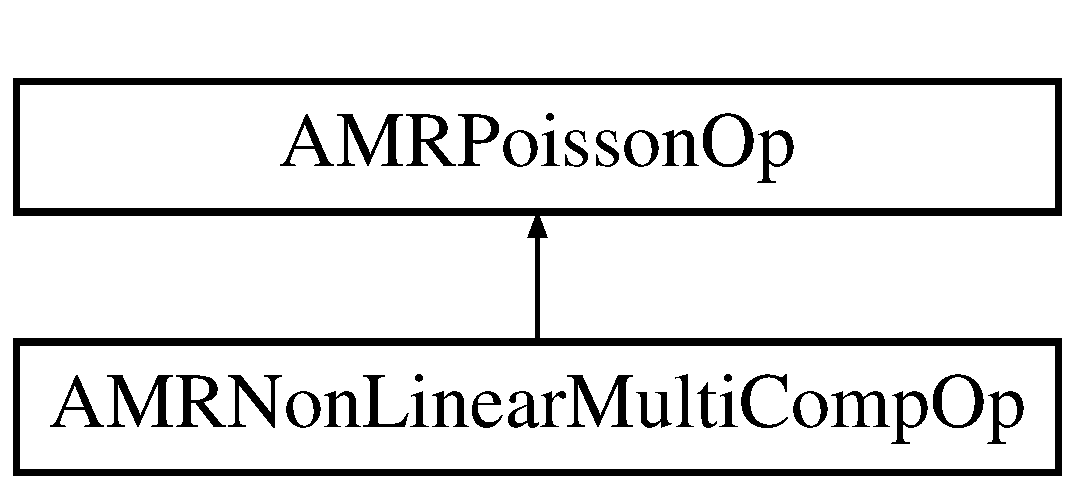
\includegraphics[height=2.000000cm]{class_a_m_r_non_linear_multi_comp_op}
\end{center}
\end{figure}
\subsection*{Public Member Functions}
\begin{DoxyCompactItemize}
\item 
void \hyperlink{class_a_m_r_non_linear_multi_comp_op_ad5c79a27d60fc17c24eea9c052aa84ac}{finer\-Operator\-Changed} (const M\-G\-Level\-Op$<$ Level\-Data$<$ F\-Array\-Box $>$ $>$ \&a\-\_\-operator, int a\-\_\-coarsening\-Factor)
\item 
\hypertarget{class_a_m_r_non_linear_multi_comp_op_a639364f5cf0da9ec0237241639ae8404}{Level\-Data$<$ F\-Array\-Box $>$ \& \hyperlink{class_a_m_r_non_linear_multi_comp_op_a639364f5cf0da9ec0237241639ae8404}{identity\-Coef} ()}\label{class_a_m_r_non_linear_multi_comp_op_a639364f5cf0da9ec0237241639ae8404}

\begin{DoxyCompactList}\small\item\em Returns identity coefficient data. \end{DoxyCompactList}\item 
void \hyperlink{class_a_m_r_non_linear_multi_comp_op_a64125ca23b133e2ca86437d7b8cfad3c}{set\-B\-Coef\-Interpolator} (Ref\-Counted\-Ptr$<$ \hyperlink{class_coefficient_interpolator_linear_face}{Coefficient\-Interpolator\-Linear\-Face} $>$ \&a\-\_\-b\-Coef\-Interpolator)
\item 
void \hyperlink{class_a_m_r_non_linear_multi_comp_op_afbc2843a557aa21ae1e88372dae80f9b}{set\-A\-Coef\-Interpolator} (Ref\-Counted\-Ptr$<$ \hyperlink{class_coefficient_interpolator_linear}{Coefficient\-Interpolator\-Linear} $>$ \&a\-\_\-a\-Coef\-Interpolator)
\item 
\hypertarget{class_a_m_r_non_linear_multi_comp_op_a58e58cbf6a60f356392931aaf4d6c268}{Level\-Data$<$ Flux\-Box $>$ \& \hyperlink{class_a_m_r_non_linear_multi_comp_op_a58e58cbf6a60f356392931aaf4d6c268}{B\-Coef} ()}\label{class_a_m_r_non_linear_multi_comp_op_a58e58cbf6a60f356392931aaf4d6c268}

\begin{DoxyCompactList}\small\item\em Returns the B coefficient. \end{DoxyCompactList}\item 
\hypertarget{class_a_m_r_non_linear_multi_comp_op_a15f72d25367f2a9a8c8a5211357947d0}{Ref\-Counted\-Ptr\\*
$<$ \hyperlink{class_coefficient_interpolator_linear_face}{Coefficient\-Interpolator\-Linear\-Face} $>$ \hyperlink{class_a_m_r_non_linear_multi_comp_op_a15f72d25367f2a9a8c8a5211357947d0}{B\-Coef\-Interpolator} ()}\label{class_a_m_r_non_linear_multi_comp_op_a15f72d25367f2a9a8c8a5211357947d0}

\begin{DoxyCompactList}\small\item\em Allows access to the B coefficient interpolator. \end{DoxyCompactList}\item 
\hypertarget{class_a_m_r_non_linear_multi_comp_op_a3f2f1e5860115bff0d72527de816bc64}{Ref\-Counted\-Ptr\\*
$<$ \hyperlink{class_coefficient_interpolator_linear}{Coefficient\-Interpolator\-Linear} $>$ \hyperlink{class_a_m_r_non_linear_multi_comp_op_a3f2f1e5860115bff0d72527de816bc64}{A\-Coef\-Interpolator} ()}\label{class_a_m_r_non_linear_multi_comp_op_a3f2f1e5860115bff0d72527de816bc64}

\begin{DoxyCompactList}\small\item\em Allows access to the A coefficient interpolator. \end{DoxyCompactList}\item 
void \hyperlink{class_a_m_r_non_linear_multi_comp_op_afb810f3b1d7826edd752a2d90264cc8e}{set\-Time} (Real a\-\_\-time)
\item 
\hypertarget{class_a_m_r_non_linear_multi_comp_op_a8a43737a8d5fe5805ebbf3d72388df9b}{void \hyperlink{class_a_m_r_non_linear_multi_comp_op_a8a43737a8d5fe5805ebbf3d72388df9b}{compute\-Diffused\-Var} (Level\-Data$<$ F\-Array\-Box $>$ \&liquid\-Conc, const Level\-Data$<$ F\-Array\-Box $>$ \&bulk\-Conc, bool a\-\_\-homogeneous=false)}\label{class_a_m_r_non_linear_multi_comp_op_a8a43737a8d5fe5805ebbf3d72388df9b}

\begin{DoxyCompactList}\small\item\em Compute temperature, liquid concentration from enthalpy, bulk concentration etc. \end{DoxyCompactList}\item 
\hypertarget{class_a_m_r_non_linear_multi_comp_op_a7100d4ee1ab6e020e6fe62522c762b18}{virtual void \hyperlink{class_a_m_r_non_linear_multi_comp_op_a7100d4ee1ab6e020e6fe62522c762b18}{compute\-Diffused\-Var} (F\-Array\-Box \&a\-\_\-calculated\-Var, const F\-Array\-Box \&a\-\_\-primary\-Var, const Data\-Index dit, bool a\-\_\-homogeneous=false)}\label{class_a_m_r_non_linear_multi_comp_op_a7100d4ee1ab6e020e6fe62522c762b18}

\begin{DoxyCompactList}\small\item\em Compute temperature, liquid concentration from enthalpy, bulk concentration etc. \end{DoxyCompactList}\end{DoxyCompactItemize}
\begin{Indent}{\bf A\-M\-R\-Non\-Linear\-Multi\-Comp\-Op functions}\par
\begin{DoxyCompactItemize}
\item 
\hypertarget{class_a_m_r_non_linear_multi_comp_op_a2205291922bf767821fcbeb13f52a338}{{\bfseries A\-M\-R\-Non\-Linear\-Multi\-Comp\-Op} ()}\label{class_a_m_r_non_linear_multi_comp_op_a2205291922bf767821fcbeb13f52a338}

\item 
\hypertarget{class_a_m_r_non_linear_multi_comp_op_a6f358cdb028df9d5a9d274fda7c77a77}{virtual {\bfseries $\sim$\-A\-M\-R\-Non\-Linear\-Multi\-Comp\-Op} ()}\label{class_a_m_r_non_linear_multi_comp_op_a6f358cdb028df9d5a9d274fda7c77a77}

\item 
\hypertarget{class_a_m_r_non_linear_multi_comp_op_a8c6014f3d9208f5184d09d700876335b}{virtual void \hyperlink{class_a_m_r_non_linear_multi_comp_op_a8c6014f3d9208f5184d09d700876335b}{residual\-I} (Level\-Data$<$ F\-Array\-Box $>$ \&a\-\_\-lhs, const Level\-Data$<$ F\-Array\-Box $>$ \&a\-\_\-phi, const Level\-Data$<$ F\-Array\-Box $>$ \&a\-\_\-rhs, bool a\-\_\-homogeneous=false)}\label{class_a_m_r_non_linear_multi_comp_op_a8c6014f3d9208f5184d09d700876335b}

\begin{DoxyCompactList}\small\item\em Compute residual. \end{DoxyCompactList}\item 
\hypertarget{class_a_m_r_non_linear_multi_comp_op_aef99970c9405719bde322dde73ba1aff}{virtual void \hyperlink{class_a_m_r_non_linear_multi_comp_op_aef99970c9405719bde322dde73ba1aff}{pre\-Cond} (Level\-Data$<$ F\-Array\-Box $>$ \&a\-\_\-correction, const Level\-Data$<$ F\-Array\-Box $>$ \&a\-\_\-residual)}\label{class_a_m_r_non_linear_multi_comp_op_aef99970c9405719bde322dde73ba1aff}

\begin{DoxyCompactList}\small\item\em Preconditioner. \end{DoxyCompactList}\item 
\hypertarget{class_a_m_r_non_linear_multi_comp_op_a8313cc6520e242cfc9eb796038268bb6}{virtual void \hyperlink{class_a_m_r_non_linear_multi_comp_op_a8313cc6520e242cfc9eb796038268bb6}{apply\-Op\-I} (Level\-Data$<$ F\-Array\-Box $>$ \&a\-\_\-lhs, const Level\-Data$<$ F\-Array\-Box $>$ \&a\-\_\-phi, bool a\-\_\-homogeneous=false)}\label{class_a_m_r_non_linear_multi_comp_op_a8313cc6520e242cfc9eb796038268bb6}

\begin{DoxyCompactList}\small\item\em Apply operator. \end{DoxyCompactList}\item 
\hypertarget{class_a_m_r_non_linear_multi_comp_op_aa6b8a71fa8501fdb71adab30bc7d5295}{virtual void \hyperlink{class_a_m_r_non_linear_multi_comp_op_aa6b8a71fa8501fdb71adab30bc7d5295}{apply\-Op\-No\-Boundary} (Level\-Data$<$ F\-Array\-Box $>$ \&a\-\_\-lhs, const Level\-Data$<$ F\-Array\-Box $>$ \&a\-\_\-phi)}\label{class_a_m_r_non_linear_multi_comp_op_aa6b8a71fa8501fdb71adab30bc7d5295}

\begin{DoxyCompactList}\small\item\em Apply operator. \end{DoxyCompactList}\item 
\hypertarget{class_a_m_r_non_linear_multi_comp_op_a2dba9dd175512b57ac8e2a7d88a0d79c}{void \hyperlink{class_a_m_r_non_linear_multi_comp_op_a2dba9dd175512b57ac8e2a7d88a0d79c}{apply\-Op\-No\-Boundary2} (Level\-Data$<$ F\-Array\-Box $>$ \&a\-\_\-lhs, const Level\-Data$<$ F\-Array\-Box $>$ \&a\-\_\-phi, bool a\-\_\-homogeneous)}\label{class_a_m_r_non_linear_multi_comp_op_a2dba9dd175512b57ac8e2a7d88a0d79c}

\begin{DoxyCompactList}\small\item\em Apply operator. \end{DoxyCompactList}\item 
\hypertarget{class_a_m_r_non_linear_multi_comp_op_a8febdc5604ebbaabbbb09832fe829a24}{virtual void \hyperlink{class_a_m_r_non_linear_multi_comp_op_a8febdc5604ebbaabbbb09832fe829a24}{diagonal\-Scale} (Level\-Data$<$ F\-Array\-Box $>$ \&a\-\_\-rhs, bool a\-\_\-kappa\-Weighted)}\label{class_a_m_r_non_linear_multi_comp_op_a8febdc5604ebbaabbbb09832fe829a24}

\begin{DoxyCompactList}\small\item\em Scale with identity coefficient. \end{DoxyCompactList}\item 
\hypertarget{class_a_m_r_non_linear_multi_comp_op_a9b8f70f0355ad8fe044d132d5235b50d}{virtual void \hyperlink{class_a_m_r_non_linear_multi_comp_op_a9b8f70f0355ad8fe044d132d5235b50d}{divide\-By\-Identity\-Coef} (Level\-Data$<$ F\-Array\-Box $>$ \&a\-\_\-rhs)}\label{class_a_m_r_non_linear_multi_comp_op_a9b8f70f0355ad8fe044d132d5235b50d}

\begin{DoxyCompactList}\small\item\em Divide by identity coefficient. \end{DoxyCompactList}\item 
\hypertarget{class_a_m_r_non_linear_multi_comp_op_a78c046aa738c5edede492bf14ef913de}{virtual void \hyperlink{class_a_m_r_non_linear_multi_comp_op_a78c046aa738c5edede492bf14ef913de}{set\-Alpha\-And\-Beta} (const Real \&a\-\_\-alpha, const Real \&a\-\_\-beta)}\label{class_a_m_r_non_linear_multi_comp_op_a78c046aa738c5edede492bf14ef913de}

\begin{DoxyCompactList}\small\item\em For tga stuff. \end{DoxyCompactList}\item 
\hypertarget{class_a_m_r_non_linear_multi_comp_op_a6029b152d2e8faddbf820f188cb73c01}{virtual void \hyperlink{class_a_m_r_non_linear_multi_comp_op_a6029b152d2e8faddbf820f188cb73c01}{set\-Coefs} (const Ref\-Counted\-Ptr$<$ Level\-Data$<$ F\-Array\-Box $>$ $>$ \&a\-\_\-a\-Coef, const Ref\-Counted\-Ptr$<$ Level\-Data$<$ Flux\-Box $>$ $>$ \&a\-\_\-b\-Coef, const Real \&a\-\_\-alpha, const Real \&a\-\_\-beta)}\label{class_a_m_r_non_linear_multi_comp_op_a6029b152d2e8faddbf820f188cb73c01}

\begin{DoxyCompactList}\small\item\em Also calls reset lambda. \end{DoxyCompactList}\item 
\hypertarget{class_a_m_r_non_linear_multi_comp_op_aa558902d2bd88e41dff404c6b3ae206f}{virtual void \hyperlink{class_a_m_r_non_linear_multi_comp_op_aa558902d2bd88e41dff404c6b3ae206f}{reset\-Lambda} ()}\label{class_a_m_r_non_linear_multi_comp_op_aa558902d2bd88e41dff404c6b3ae206f}

\begin{DoxyCompactList}\small\item\em Should be called before the relaxation parameter is needed. \end{DoxyCompactList}\item 
\hypertarget{class_a_m_r_non_linear_multi_comp_op_ad3c8e757a15bb3fdfa03c7b0c05315df}{void \hyperlink{class_a_m_r_non_linear_multi_comp_op_ad3c8e757a15bb3fdfa03c7b0c05315df}{reset\-Lambda\-Non\-Linear} (const Level\-Data$<$ F\-Array\-Box $>$ \&a\-\_\-phi)}\label{class_a_m_r_non_linear_multi_comp_op_ad3c8e757a15bb3fdfa03c7b0c05315df}

\begin{DoxyCompactList}\small\item\em Recalculate lambda for nonlinear calculations (not actually current used) \end{DoxyCompactList}\item 
\hypertarget{class_a_m_r_non_linear_multi_comp_op_a4fe4520a51b78a009eba0cde433949dd}{virtual void \hyperlink{class_a_m_r_non_linear_multi_comp_op_a4fe4520a51b78a009eba0cde433949dd}{compute\-Lambda} ()}\label{class_a_m_r_non_linear_multi_comp_op_a4fe4520a51b78a009eba0cde433949dd}

\begin{DoxyCompactList}\small\item\em Compute lambda once alpha, a\-Coef, beta, b\-Coef are defined. \end{DoxyCompactList}\item 
\hypertarget{class_a_m_r_non_linear_multi_comp_op_a2fb72537fbed147bb56f3eea440746ea}{virtual void \hyperlink{class_a_m_r_non_linear_multi_comp_op_a2fb72537fbed147bb56f3eea440746ea}{reflux} (const Level\-Data$<$ F\-Array\-Box $>$ \&a\-\_\-phi\-Fine, const Level\-Data$<$ F\-Array\-Box $>$ \&a\-\_\-phi, Level\-Data$<$ F\-Array\-Box $>$ \&a\-\_\-residual, A\-M\-R\-Level\-Op$<$ Level\-Data$<$ F\-Array\-Box $>$ $>$ $\ast$a\-\_\-finer\-Op)}\label{class_a_m_r_non_linear_multi_comp_op_a2fb72537fbed147bb56f3eea440746ea}

\begin{DoxyCompactList}\small\item\em Increment flux registers and calculate reflux. \end{DoxyCompactList}\item 
virtual void \hyperlink{class_a_m_r_non_linear_multi_comp_op_a348203bd1783a1ce09fb8dbf876d79ae}{get\-Flux} (Flux\-Box \&a\-\_\-flux, const Level\-Data$<$ F\-Array\-Box $>$ \&a\-\_\-data, const Box \&a\-\_\-grid, const Data\-Index \&a\-\_\-dit, Real a\-\_\-scale)
\begin{DoxyCompactList}\small\item\em get\-Flux function which matches interface to A\-M\-R\-Poisson\-Op \end{DoxyCompactList}\item 
\hypertarget{class_a_m_r_non_linear_multi_comp_op_ab3b9ca0576f197409ff893e598a286d0}{virtual void \hyperlink{class_a_m_r_non_linear_multi_comp_op_ab3b9ca0576f197409ff893e598a286d0}{get\-Flux} (Flux\-Box \&a\-\_\-flux, const Level\-Data$<$ F\-Array\-Box $>$ \&a\-\_\-data, const Flux\-Box \&a\-\_\-b\-Coef, const Box \&a\-\_\-grid, const Data\-Index \&a\-\_\-dit, Real a\-\_\-scale)}\label{class_a_m_r_non_linear_multi_comp_op_ab3b9ca0576f197409ff893e598a286d0}

\begin{DoxyCompactList}\small\item\em get diffusive flux \end{DoxyCompactList}\end{DoxyCompactItemize}
\end{Indent}
\begin{Indent}{\bf M\-G\-Level\-Op functions}\par
{\em \subsection*{$<$$<$$<$$<$$<$$<$$<$ \hyperlink{_a_m_r_non_linear_multi_comp_op_8_h_source}{A\-M\-R\-Non\-Linear\-Multi\-Comp\-Op.\-H} }}\begin{DoxyCompactItemize}
\item 
virtual void \hyperlink{class_a_m_r_non_linear_multi_comp_op_ad0f58cb65ab237d61874f2aeae1a4da3}{restrict\-Residual} (Level\-Data$<$ F\-Array\-Box $>$ \&a\-\_\-res\-Coarse, Level\-Data$<$ F\-Array\-Box $>$ \&a\-\_\-phi\-Fine, const Level\-Data$<$ F\-Array\-Box $>$ \&a\-\_\-rhs\-Fine)
\begin{DoxyCompactList}\small\item\em calculate restricted residual \end{DoxyCompactList}\item 
\hypertarget{class_a_m_r_non_linear_multi_comp_op_a65b95bc4127ffdfab47bd5a81acf2772}{virtual void \hyperlink{class_a_m_r_non_linear_multi_comp_op_a65b95bc4127ffdfab47bd5a81acf2772}{restrict\-Residual} (Level\-Data$<$ F\-Array\-Box $>$ \&a\-\_\-res\-Coarse, Level\-Data$<$ F\-Array\-Box $>$ \&a\-\_\-phi\-Fine, const Level\-Data$<$ F\-Array\-Box $>$ $\ast$a\-\_\-phi\-Coarse, const Level\-Data$<$ F\-Array\-Box $>$ \&a\-\_\-rhs\-Fine, bool homogeneous)}\label{class_a_m_r_non_linear_multi_comp_op_a65b95bc4127ffdfab47bd5a81acf2772}

\begin{DoxyCompactList}\small\item\em calculate restricted residual \end{DoxyCompactList}\item 
\hypertarget{class_a_m_r_non_linear_multi_comp_op_ac3ea29dd436c89aafde25c8f33fdb30d}{virtual void \hyperlink{class_a_m_r_non_linear_multi_comp_op_ac3ea29dd436c89aafde25c8f33fdb30d}{create\-Coarser} (Level\-Data$<$ F\-Array\-Box $>$ \&a\-\_\-coarse, const Level\-Data$<$ F\-Array\-Box $>$ \&a\-\_\-fine, bool a\-\_\-ghosted)}\label{class_a_m_r_non_linear_multi_comp_op_ac3ea29dd436c89aafde25c8f33fdb30d}

\begin{DoxyCompactList}\small\item\em Create coarser version of field. \end{DoxyCompactList}\item 
\hypertarget{class_a_m_r_non_linear_multi_comp_op_a47ff0ed449857310593c55c4d192a581}{virtual void \hyperlink{class_a_m_r_non_linear_multi_comp_op_a47ff0ed449857310593c55c4d192a581}{prolong\-Increment} (Level\-Data$<$ F\-Array\-Box $>$ \&a\-\_\-phi\-This\-Level, const Level\-Data$<$ F\-Array\-Box $>$ \&a\-\_\-correct\-Coarse)}\label{class_a_m_r_non_linear_multi_comp_op_a47ff0ed449857310593c55c4d192a581}

\begin{DoxyCompactList}\small\item\em Prolong correction. \end{DoxyCompactList}\item 
\hypertarget{class_a_m_r_non_linear_multi_comp_op_a7825a1c5e9bffc3fefe6b5b7fb1458f7}{virtual void \hyperlink{class_a_m_r_non_linear_multi_comp_op_a7825a1c5e9bffc3fefe6b5b7fb1458f7}{restrict} (Level\-Data$<$ F\-Array\-Box $>$ \&a\-\_\-phi\-Coarse, const Level\-Data$<$ F\-Array\-Box $>$ \&a\-\_\-phi\-Fine)}\label{class_a_m_r_non_linear_multi_comp_op_a7825a1c5e9bffc3fefe6b5b7fb1458f7}

\begin{DoxyCompactList}\small\item\em Restrict solution to coarser level. \end{DoxyCompactList}\item 
\hypertarget{class_a_m_r_non_linear_multi_comp_op_aee81544614b579b9ca7cb03c6e92f9cd}{void \hyperlink{class_a_m_r_non_linear_multi_comp_op_aee81544614b579b9ca7cb03c6e92f9cd}{apply\-Op\-Mg} (Level\-Data$<$ F\-Array\-Box $>$ \&a\-\_\-lhs, Level\-Data$<$ F\-Array\-Box $>$ \&a\-\_\-phi, Level\-Data$<$ F\-Array\-Box $>$ $\ast$a\-\_\-phi\-Coarse, bool a\-\_\-homogeneous)}\label{class_a_m_r_non_linear_multi_comp_op_aee81544614b579b9ca7cb03c6e92f9cd}

\begin{DoxyCompactList}\small\item\em Apply operator. \end{DoxyCompactList}\end{DoxyCompactItemize}
\end{Indent}
\subsection*{Public Attributes}
\begin{DoxyCompactItemize}
\item 
\hypertarget{class_a_m_r_non_linear_multi_comp_op_af95d5785a1c0291dbd7309b1539ab2fb}{Ref\-Counted\-Ptr$<$ Level\-Data\\*
$<$ F\-Array\-Box $>$ $>$ \hyperlink{class_a_m_r_non_linear_multi_comp_op_af95d5785a1c0291dbd7309b1539ab2fb}{m\-\_\-a\-Coef}}\label{class_a_m_r_non_linear_multi_comp_op_af95d5785a1c0291dbd7309b1539ab2fb}

\begin{DoxyCompactList}\small\item\em Identity operator spatially varying coefficient storage (cell-\/centered) --- if you change this call \hyperlink{class_a_m_r_non_linear_multi_comp_op_aa558902d2bd88e41dff404c6b3ae206f}{reset\-Lambda()} \end{DoxyCompactList}\item 
\hypertarget{class_a_m_r_non_linear_multi_comp_op_a137649e6de11ed5ebf0fd06ed6766e65}{Ref\-Counted\-Ptr$<$ Level\-Data\\*
$<$ F\-Array\-Box $>$ $>$ \hyperlink{class_a_m_r_non_linear_multi_comp_op_a137649e6de11ed5ebf0fd06ed6766e65}{m\-\_\-secondary\-Var}}\label{class_a_m_r_non_linear_multi_comp_op_a137649e6de11ed5ebf0fd06ed6766e65}

\begin{DoxyCompactList}\small\item\em Which of enthalpy or bulk concentration we're not solving for. \end{DoxyCompactList}\item 
\hypertarget{class_a_m_r_non_linear_multi_comp_op_ad6cea304fd804cbf1c7340a9740ad955}{Ref\-Counted\-Ptr$<$ Level\-Data\\*
$<$ F\-Array\-Box $>$ $>$ \hyperlink{class_a_m_r_non_linear_multi_comp_op_ad6cea304fd804cbf1c7340a9740ad955}{m\-\_\-enthalpy\-Solidus}}\label{class_a_m_r_non_linear_multi_comp_op_ad6cea304fd804cbf1c7340a9740ad955}

\begin{DoxyCompactList}\small\item\em Enthalpy solidus. \end{DoxyCompactList}\item 
\hypertarget{class_a_m_r_non_linear_multi_comp_op_a285a99a0a4dcf36cd641f8c46d815873}{Ref\-Counted\-Ptr$<$ Level\-Data\\*
$<$ F\-Array\-Box $>$ $>$ \hyperlink{class_a_m_r_non_linear_multi_comp_op_a285a99a0a4dcf36cd641f8c46d815873}{m\-\_\-enthalpy\-Liquidus}}\label{class_a_m_r_non_linear_multi_comp_op_a285a99a0a4dcf36cd641f8c46d815873}

\begin{DoxyCompactList}\small\item\em Enthalpy liquidus. \end{DoxyCompactList}\item 
\hypertarget{class_a_m_r_non_linear_multi_comp_op_a84014ea27489edc10ca99fd27e3fa59b}{Ref\-Counted\-Ptr$<$ Level\-Data\\*
$<$ F\-Array\-Box $>$ $>$ \hyperlink{class_a_m_r_non_linear_multi_comp_op_a84014ea27489edc10ca99fd27e3fa59b}{m\-\_\-enthalpy\-Eutectic}}\label{class_a_m_r_non_linear_multi_comp_op_a84014ea27489edc10ca99fd27e3fa59b}

\begin{DoxyCompactList}\small\item\em Eutectic enthalpy. \end{DoxyCompactList}\item 
\hypertarget{class_a_m_r_non_linear_multi_comp_op_a84251f9cbb92946cd0eba54571ba0010}{B\-C\-Holder {\bfseries m\-\_\-diffused\-Var\-B\-C}}\label{class_a_m_r_non_linear_multi_comp_op_a84251f9cbb92946cd0eba54571ba0010}

\item 
\hypertarget{class_a_m_r_non_linear_multi_comp_op_a585689df6d0c8fe37528664bad748725}{Ref\-Counted\-Ptr$<$ Level\-Data\\*
$<$ Flux\-Box $>$ $>$ \hyperlink{class_a_m_r_non_linear_multi_comp_op_a585689df6d0c8fe37528664bad748725}{m\-\_\-b\-Coef}}\label{class_a_m_r_non_linear_multi_comp_op_a585689df6d0c8fe37528664bad748725}

\begin{DoxyCompactList}\small\item\em Laplacian operator spatially varying coefficient storage (face-\/centered) --- if you change this call \hyperlink{class_a_m_r_non_linear_multi_comp_op_aa558902d2bd88e41dff404c6b3ae206f}{reset\-Lambda()} \end{DoxyCompactList}\item 
\hypertarget{class_a_m_r_non_linear_multi_comp_op_afc96721bca344bb2d470d7f0731b4285}{Level\-Data$<$ F\-Array\-Box $>$ \hyperlink{class_a_m_r_non_linear_multi_comp_op_afc96721bca344bb2d470d7f0731b4285}{m\-\_\-lambda}}\label{class_a_m_r_non_linear_multi_comp_op_afc96721bca344bb2d470d7f0731b4285}

\begin{DoxyCompactList}\small\item\em Reciprocal of the diagonal entry of the operator matrix. \end{DoxyCompactList}\item 
\hypertarget{class_a_m_r_non_linear_multi_comp_op_aafb3edc6ac424eb1e6f7bbc9a15c1c9e}{\hyperlink{class_mushy_layer_params}{Mushy\-Layer\-Params} $\ast$ \hyperlink{class_a_m_r_non_linear_multi_comp_op_aafb3edc6ac424eb1e6f7bbc9a15c1c9e}{m\-\_\-params}}\label{class_a_m_r_non_linear_multi_comp_op_aafb3edc6ac424eb1e6f7bbc9a15c1c9e}

\begin{DoxyCompactList}\small\item\em Physical parameters for problems. \end{DoxyCompactList}\item 
bool \hyperlink{class_a_m_r_non_linear_multi_comp_op_a56ee2a89dc1bce9701951d48633fc808}{m\-\_\-\-F\-A\-S}
\begin{DoxyCompactList}\small\item\em Object to compute enthalpy method variables. \end{DoxyCompactList}\end{DoxyCompactItemize}
\subsection*{Protected Member Functions}
\begin{DoxyCompactItemize}
\item 
\hypertarget{class_a_m_r_non_linear_multi_comp_op_a8ec4d6960ca7282d700aa370b3ce875e}{virtual void \hyperlink{class_a_m_r_non_linear_multi_comp_op_a8ec4d6960ca7282d700aa370b3ce875e}{level\-G\-S\-R\-B} (Level\-Data$<$ F\-Array\-Box $>$ \&a\-\_\-phi, const Level\-Data$<$ F\-Array\-Box $>$ \&a\-\_\-rhs)}\label{class_a_m_r_non_linear_multi_comp_op_a8ec4d6960ca7282d700aa370b3ce875e}

\begin{DoxyCompactList}\small\item\em Gauss-\/seidel relaxation. \end{DoxyCompactList}\item 
\hypertarget{class_a_m_r_non_linear_multi_comp_op_a68cf60aeb967af9a3c7e1c628d7969f2}{virtual void \hyperlink{class_a_m_r_non_linear_multi_comp_op_a68cf60aeb967af9a3c7e1c628d7969f2}{level\-Multi\-Color} (Level\-Data$<$ F\-Array\-Box $>$ \&a\-\_\-phi, const Level\-Data$<$ F\-Array\-Box $>$ \&a\-\_\-rhs)}\label{class_a_m_r_non_linear_multi_comp_op_a68cf60aeb967af9a3c7e1c628d7969f2}

\begin{DoxyCompactList}\small\item\em Multicolor relaxation. \end{DoxyCompactList}\item 
\hypertarget{class_a_m_r_non_linear_multi_comp_op_a2bb1423e981bdf7357bc3faab3385908}{virtual void \hyperlink{class_a_m_r_non_linear_multi_comp_op_a2bb1423e981bdf7357bc3faab3385908}{loose\-G\-S\-R\-B} (Level\-Data$<$ F\-Array\-Box $>$ \&a\-\_\-phi, const Level\-Data$<$ F\-Array\-Box $>$ \&a\-\_\-rhs)}\label{class_a_m_r_non_linear_multi_comp_op_a2bb1423e981bdf7357bc3faab3385908}

\begin{DoxyCompactList}\small\item\em Gauss-\/seidel relaxation. \end{DoxyCompactList}\item 
\hypertarget{class_a_m_r_non_linear_multi_comp_op_a123577c271aa45f550fbc159b03a144c}{virtual void \hyperlink{class_a_m_r_non_linear_multi_comp_op_a123577c271aa45f550fbc159b03a144c}{overlap\-G\-S\-R\-B} (Level\-Data$<$ F\-Array\-Box $>$ \&a\-\_\-phi, const Level\-Data$<$ F\-Array\-Box $>$ \&a\-\_\-rhs)}\label{class_a_m_r_non_linear_multi_comp_op_a123577c271aa45f550fbc159b03a144c}

\begin{DoxyCompactList}\small\item\em Gauss-\/seidel relaxation. \end{DoxyCompactList}\item 
\hypertarget{class_a_m_r_non_linear_multi_comp_op_a301f4fedc4fed7a13e914d5f26f8d719}{virtual void \hyperlink{class_a_m_r_non_linear_multi_comp_op_a301f4fedc4fed7a13e914d5f26f8d719}{level\-G\-S\-R\-B\-Lazy} (Level\-Data$<$ F\-Array\-Box $>$ \&a\-\_\-phi, const Level\-Data$<$ F\-Array\-Box $>$ \&a\-\_\-rhs)}\label{class_a_m_r_non_linear_multi_comp_op_a301f4fedc4fed7a13e914d5f26f8d719}

\begin{DoxyCompactList}\small\item\em Gauss-\/seidel relaxation. \end{DoxyCompactList}\item 
\hypertarget{class_a_m_r_non_linear_multi_comp_op_a7fd508a366d0e779e8ac82ca7f03ec69}{virtual void \hyperlink{class_a_m_r_non_linear_multi_comp_op_a7fd508a366d0e779e8ac82ca7f03ec69}{level\-Jacobi} (Level\-Data$<$ F\-Array\-Box $>$ \&a\-\_\-phi, const Level\-Data$<$ F\-Array\-Box $>$ \&a\-\_\-rhs)}\label{class_a_m_r_non_linear_multi_comp_op_a7fd508a366d0e779e8ac82ca7f03ec69}

\begin{DoxyCompactList}\small\item\em Jacobi relaxation. \end{DoxyCompactList}\item 
\hypertarget{class_a_m_r_non_linear_multi_comp_op_aa97fbc9429f251b8d61722652547822f}{virtual void \hyperlink{class_a_m_r_non_linear_multi_comp_op_aa97fbc9429f251b8d61722652547822f}{get\-Flux} (F\-Array\-Box \&a\-\_\-flux, const F\-Array\-Box \&a\-\_\-data, const Flux\-Box \&a\-\_\-b\-Coef, const Box \&a\-\_\-facebox, int a\-\_\-dir, const Data\-Index \&a\-\_\-dit, int a\-\_\-ref=1) const }\label{class_a_m_r_non_linear_multi_comp_op_aa97fbc9429f251b8d61722652547822f}

\begin{DoxyCompactList}\small\item\em computes flux over face-\/centered a\-\_\-facebox. \end{DoxyCompactList}\end{DoxyCompactItemize}
\subsection*{Protected Attributes}
\begin{DoxyCompactItemize}
\item 
\hypertarget{class_a_m_r_non_linear_multi_comp_op_a15ba0831b7d6ed8509954fcdedbc68b2}{Layout\-Data$<$ C\-F\-I\-V\-S $>$ \hyperlink{class_a_m_r_non_linear_multi_comp_op_a15ba0831b7d6ed8509954fcdedbc68b2}{m\-\_\-lo\-C\-F\-I\-V\-S} \mbox{[}Space\-Dim\mbox{]}}\label{class_a_m_r_non_linear_multi_comp_op_a15ba0831b7d6ed8509954fcdedbc68b2}

\begin{DoxyCompactList}\small\item\em Intvects on coarse-\/fine interfaces. \end{DoxyCompactList}\item 
\hypertarget{class_a_m_r_non_linear_multi_comp_op_ad98133545fea83f7ea83d97b571864ab}{Layout\-Data$<$ C\-F\-I\-V\-S $>$ \hyperlink{class_a_m_r_non_linear_multi_comp_op_ad98133545fea83f7ea83d97b571864ab}{m\-\_\-hi\-C\-F\-I\-V\-S} \mbox{[}Space\-Dim\mbox{]}}\label{class_a_m_r_non_linear_multi_comp_op_ad98133545fea83f7ea83d97b571864ab}

\begin{DoxyCompactList}\small\item\em Intvects on coarse-\/fine interfaces. \end{DoxyCompactList}\item 
\hypertarget{class_a_m_r_non_linear_multi_comp_op_a355e5cdcad525f983a8122bcf0ab09b4}{Ref\-Counted\-Ptr\\*
$<$ \hyperlink{class_coefficient_interpolator_linear_face}{Coefficient\-Interpolator\-Linear\-Face} $>$ \hyperlink{class_a_m_r_non_linear_multi_comp_op_a355e5cdcad525f983a8122bcf0ab09b4}{m\-\_\-b\-Coef\-Interpolator}}\label{class_a_m_r_non_linear_multi_comp_op_a355e5cdcad525f983a8122bcf0ab09b4}

\begin{DoxyCompactList}\small\item\em Interpolator for b coefficient data. \end{DoxyCompactList}\item 
\hypertarget{class_a_m_r_non_linear_multi_comp_op_a725b0c0f13966b9b4ef303219a25fe7d}{Ref\-Counted\-Ptr\\*
$<$ \hyperlink{class_coefficient_interpolator_linear}{Coefficient\-Interpolator\-Linear} $>$ \hyperlink{class_a_m_r_non_linear_multi_comp_op_a725b0c0f13966b9b4ef303219a25fe7d}{m\-\_\-a\-Coef\-Interpolator}}\label{class_a_m_r_non_linear_multi_comp_op_a725b0c0f13966b9b4ef303219a25fe7d}

\begin{DoxyCompactList}\small\item\em Interpolator for a coefficient data. \end{DoxyCompactList}\item 
\hypertarget{class_a_m_r_non_linear_multi_comp_op_a70bf32d1723de157b96d70bd53d2f255}{Real \hyperlink{class_a_m_r_non_linear_multi_comp_op_a70bf32d1723de157b96d70bd53d2f255}{m\-\_\-time}}\label{class_a_m_r_non_linear_multi_comp_op_a70bf32d1723de157b96d70bd53d2f255}

\begin{DoxyCompactList}\small\item\em Current time. \end{DoxyCompactList}\item 
\hypertarget{class_a_m_r_non_linear_multi_comp_op_a799454b3424eebb1f152b131cf6ea1f4}{bool \hyperlink{class_a_m_r_non_linear_multi_comp_op_a799454b3424eebb1f152b131cf6ea1f4}{m\-\_\-lambda\-Needs\-Resetting}}\label{class_a_m_r_non_linear_multi_comp_op_a799454b3424eebb1f152b131cf6ea1f4}

\begin{DoxyCompactList}\small\item\em Does the relaxation coefficient need to be reset? \end{DoxyCompactList}\end{DoxyCompactItemize}


\subsection{Detailed Description}
Nonlinear variable coefficient operator. 

Operator for solving variable-\/coefficient (alpha $\ast$ a\-Coef(x) $\ast$ I -\/ beta $\ast$ Div(b\-Coef(x) . Grad)) phi = rho over an A\-M\-R hierarchy. 

\subsection{Member Function Documentation}
\hypertarget{class_a_m_r_non_linear_multi_comp_op_ad5c79a27d60fc17c24eea9c052aa84ac}{\index{A\-M\-R\-Non\-Linear\-Multi\-Comp\-Op@{A\-M\-R\-Non\-Linear\-Multi\-Comp\-Op}!finer\-Operator\-Changed@{finer\-Operator\-Changed}}
\index{finer\-Operator\-Changed@{finer\-Operator\-Changed}!AMRNonLinearMultiCompOp@{A\-M\-R\-Non\-Linear\-Multi\-Comp\-Op}}
\subsubsection[{finer\-Operator\-Changed}]{\setlength{\rightskip}{0pt plus 5cm}void A\-M\-R\-Non\-Linear\-Multi\-Comp\-Op\-::finer\-Operator\-Changed (
\begin{DoxyParamCaption}
\item[{const M\-G\-Level\-Op$<$ Level\-Data$<$ F\-Array\-Box $>$ $>$ \&}]{a\-\_\-operator, }
\item[{int}]{a\-\_\-coarsening\-Factor}
\end{DoxyParamCaption}
)}}\label{class_a_m_r_non_linear_multi_comp_op_ad5c79a27d60fc17c24eea9c052aa84ac}
Has finer operator changed? This is called on multigrid operators when their A\-M\-R operators are altered. \hypertarget{class_a_m_r_non_linear_multi_comp_op_a348203bd1783a1ce09fb8dbf876d79ae}{\index{A\-M\-R\-Non\-Linear\-Multi\-Comp\-Op@{A\-M\-R\-Non\-Linear\-Multi\-Comp\-Op}!get\-Flux@{get\-Flux}}
\index{get\-Flux@{get\-Flux}!AMRNonLinearMultiCompOp@{A\-M\-R\-Non\-Linear\-Multi\-Comp\-Op}}
\subsubsection[{get\-Flux}]{\setlength{\rightskip}{0pt plus 5cm}virtual void A\-M\-R\-Non\-Linear\-Multi\-Comp\-Op\-::get\-Flux (
\begin{DoxyParamCaption}
\item[{Flux\-Box \&}]{a\-\_\-flux, }
\item[{const Level\-Data$<$ F\-Array\-Box $>$ \&}]{a\-\_\-data, }
\item[{const Box \&}]{a\-\_\-grid, }
\item[{const Data\-Index \&}]{a\-\_\-dit, }
\item[{Real}]{a\-\_\-scale}
\end{DoxyParamCaption}
)\hspace{0.3cm}{\ttfamily [inline]}, {\ttfamily [virtual]}}}\label{class_a_m_r_non_linear_multi_comp_op_a348203bd1783a1ce09fb8dbf876d79ae}


get\-Flux function which matches interface to A\-M\-R\-Poisson\-Op 

assumes we want to use member-\/data b\-Coef, then calls second get\-Flux function Note that a\-\_\-data is the thing we take the gradient of, i.\-e. we calculate $ \chi \nabla \phi $ where $ \phi $ is a\-\_\-data. a\-\_\-data is N\-O\-T the bulk concentration or enthalpy \hypertarget{class_a_m_r_non_linear_multi_comp_op_ad0f58cb65ab237d61874f2aeae1a4da3}{\index{A\-M\-R\-Non\-Linear\-Multi\-Comp\-Op@{A\-M\-R\-Non\-Linear\-Multi\-Comp\-Op}!restrict\-Residual@{restrict\-Residual}}
\index{restrict\-Residual@{restrict\-Residual}!AMRNonLinearMultiCompOp@{A\-M\-R\-Non\-Linear\-Multi\-Comp\-Op}}
\subsubsection[{restrict\-Residual}]{\setlength{\rightskip}{0pt plus 5cm}void A\-M\-R\-Non\-Linear\-Multi\-Comp\-Op\-::restrict\-Residual (
\begin{DoxyParamCaption}
\item[{Level\-Data$<$ F\-Array\-Box $>$ \&}]{a\-\_\-res\-Coarse, }
\item[{Level\-Data$<$ F\-Array\-Box $>$ \&}]{a\-\_\-phi\-Fine, }
\item[{const Level\-Data$<$ F\-Array\-Box $>$ \&}]{a\-\_\-rhs\-Fine}
\end{DoxyParamCaption}
)\hspace{0.3cm}{\ttfamily [virtual]}}}\label{class_a_m_r_non_linear_multi_comp_op_ad0f58cb65ab237d61874f2aeae1a4da3}


calculate restricted residual 

a\-\_\-res\-Coarse\mbox{[}2h\mbox{]} = I\mbox{[}h-\/$>$2h\mbox{]} (rhs\-Fine\mbox{[}h\mbox{]} -\/ L\mbox{[}h\mbox{]}(phi\-Fine\mbox{[}h\mbox{]}) \hypertarget{class_a_m_r_non_linear_multi_comp_op_afbc2843a557aa21ae1e88372dae80f9b}{\index{A\-M\-R\-Non\-Linear\-Multi\-Comp\-Op@{A\-M\-R\-Non\-Linear\-Multi\-Comp\-Op}!set\-A\-Coef\-Interpolator@{set\-A\-Coef\-Interpolator}}
\index{set\-A\-Coef\-Interpolator@{set\-A\-Coef\-Interpolator}!AMRNonLinearMultiCompOp@{A\-M\-R\-Non\-Linear\-Multi\-Comp\-Op}}
\subsubsection[{set\-A\-Coef\-Interpolator}]{\setlength{\rightskip}{0pt plus 5cm}void A\-M\-R\-Non\-Linear\-Multi\-Comp\-Op\-::set\-A\-Coef\-Interpolator (
\begin{DoxyParamCaption}
\item[{Ref\-Counted\-Ptr$<$ {\bf Coefficient\-Interpolator\-Linear} $>$ \&}]{a\-\_\-a\-Coef\-Interpolator}
\end{DoxyParamCaption}
)\hspace{0.3cm}{\ttfamily [inline]}}}\label{class_a_m_r_non_linear_multi_comp_op_afbc2843a557aa21ae1e88372dae80f9b}
Sets up a model that modifies a coefficient data when the operator's time is set. 
\begin{DoxyParams}{Parameters}
{\em a\-\_\-a\-Coef\-Interpolator} & A Coefficient\-Interpolator that will be used to compute the a coefficient at specific times. \\
\hline
\end{DoxyParams}
\hypertarget{class_a_m_r_non_linear_multi_comp_op_a64125ca23b133e2ca86437d7b8cfad3c}{\index{A\-M\-R\-Non\-Linear\-Multi\-Comp\-Op@{A\-M\-R\-Non\-Linear\-Multi\-Comp\-Op}!set\-B\-Coef\-Interpolator@{set\-B\-Coef\-Interpolator}}
\index{set\-B\-Coef\-Interpolator@{set\-B\-Coef\-Interpolator}!AMRNonLinearMultiCompOp@{A\-M\-R\-Non\-Linear\-Multi\-Comp\-Op}}
\subsubsection[{set\-B\-Coef\-Interpolator}]{\setlength{\rightskip}{0pt plus 5cm}void A\-M\-R\-Non\-Linear\-Multi\-Comp\-Op\-::set\-B\-Coef\-Interpolator (
\begin{DoxyParamCaption}
\item[{Ref\-Counted\-Ptr$<$ {\bf Coefficient\-Interpolator\-Linear\-Face} $>$ \&}]{a\-\_\-b\-Coef\-Interpolator}
\end{DoxyParamCaption}
)\hspace{0.3cm}{\ttfamily [inline]}}}\label{class_a_m_r_non_linear_multi_comp_op_a64125ca23b133e2ca86437d7b8cfad3c}
Sets up a model that modifies b coefficient data when the operator's time is set. 
\begin{DoxyParams}{Parameters}
{\em a\-\_\-b\-Coef\-Interpolator} & A Coefficient\-Interpolator that will be used to compute the b coefficient at specific times. \\
\hline
\end{DoxyParams}
\hypertarget{class_a_m_r_non_linear_multi_comp_op_afb810f3b1d7826edd752a2d90264cc8e}{\index{A\-M\-R\-Non\-Linear\-Multi\-Comp\-Op@{A\-M\-R\-Non\-Linear\-Multi\-Comp\-Op}!set\-Time@{set\-Time}}
\index{set\-Time@{set\-Time}!AMRNonLinearMultiCompOp@{A\-M\-R\-Non\-Linear\-Multi\-Comp\-Op}}
\subsubsection[{set\-Time}]{\setlength{\rightskip}{0pt plus 5cm}void A\-M\-R\-Non\-Linear\-Multi\-Comp\-Op\-::set\-Time (
\begin{DoxyParamCaption}
\item[{Real}]{a\-\_\-time}
\end{DoxyParamCaption}
)}}\label{class_a_m_r_non_linear_multi_comp_op_afb810f3b1d7826edd752a2d90264cc8e}
Sets the time centering of the operator. This interpolates b coefficient data at the given time if an interpolator is set. 

\subsection{Member Data Documentation}
\hypertarget{class_a_m_r_non_linear_multi_comp_op_a56ee2a89dc1bce9701951d48633fc808}{\index{A\-M\-R\-Non\-Linear\-Multi\-Comp\-Op@{A\-M\-R\-Non\-Linear\-Multi\-Comp\-Op}!m\-\_\-\-F\-A\-S@{m\-\_\-\-F\-A\-S}}
\index{m\-\_\-\-F\-A\-S@{m\-\_\-\-F\-A\-S}!AMRNonLinearMultiCompOp@{A\-M\-R\-Non\-Linear\-Multi\-Comp\-Op}}
\subsubsection[{m\-\_\-\-F\-A\-S}]{\setlength{\rightskip}{0pt plus 5cm}bool A\-M\-R\-Non\-Linear\-Multi\-Comp\-Op\-::m\-\_\-\-F\-A\-S}}\label{class_a_m_r_non_linear_multi_comp_op_a56ee2a89dc1bce9701951d48633fc808}


Object to compute enthalpy method variables. 

Boundary conditions for porosity true if we're running in F\-A\-S mode (much quicker for nonlinear problems) 

The documentation for this class was generated from the following files\-:\begin{DoxyCompactItemize}
\item 
/home/parkinsonjl/mushy-\/layer/src/A\-M\-R\-Non\-Linear\-Multi\-Comp\-Op.\-H\item 
/home/parkinsonjl/mushy-\/layer/src/A\-M\-R\-Non\-Linear\-Multi\-Comp\-Op.\-cpp\end{DoxyCompactItemize}

\hypertarget{class_a_m_r_non_linear_multi_comp_op_factory}{\section{A\-M\-R\-Non\-Linear\-Multi\-Comp\-Op\-Factory Class Reference}
\label{class_a_m_r_non_linear_multi_comp_op_factory}\index{A\-M\-R\-Non\-Linear\-Multi\-Comp\-Op\-Factory@{A\-M\-R\-Non\-Linear\-Multi\-Comp\-Op\-Factory}}
}


Factory for nonlinear variable coefficient operator.  




{\ttfamily \#include $<$A\-M\-R\-Non\-Linear\-Multi\-Comp\-Op.\-H$>$}

Inheritance diagram for A\-M\-R\-Non\-Linear\-Multi\-Comp\-Op\-Factory\-:\begin{figure}[H]
\begin{center}
\leavevmode
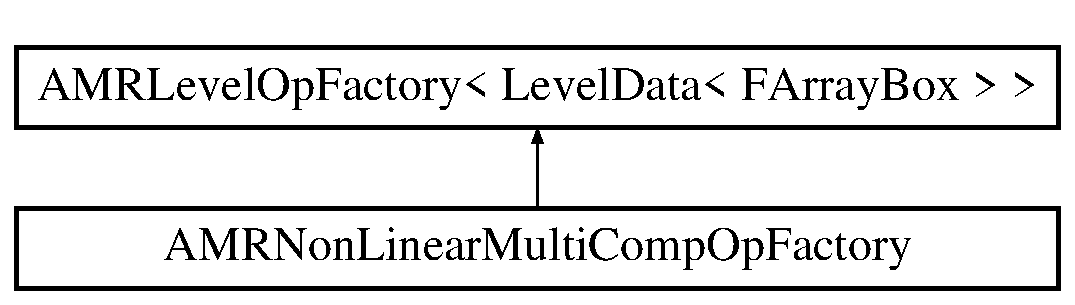
\includegraphics[height=2.000000cm]{class_a_m_r_non_linear_multi_comp_op_factory}
\end{center}
\end{figure}
\subsection*{Public Member Functions}
\begin{DoxyCompactItemize}
\item 
void \hyperlink{class_a_m_r_non_linear_multi_comp_op_factory_a197bda0900c2f6315d509a8176b738df}{define} (const Problem\-Domain \&a\-\_\-coarse\-Domain, const Vector$<$ Disjoint\-Box\-Layout $>$ \&a\-\_\-grids, const Vector$<$ int $>$ \&a\-\_\-ref\-Ratios, const Real \&a\-\_\-coarsedx, B\-C\-Holder a\-\_\-bc, const Real \&a\-\_\-alpha, Vector$<$ Ref\-Counted\-Ptr$<$ Level\-Data$<$ F\-Array\-Box $>$ $>$ $>$ \&a\-\_\-a\-Coef, const Real \&a\-\_\-beta, Vector$<$ Ref\-Counted\-Ptr$<$ Level\-Data$<$ Flux\-Box $>$ $>$ $>$ \&a\-\_\-b\-Coef, Vector$<$ Ref\-Counted\-Ptr$<$ Level\-Data$<$ F\-Array\-Box $>$ $>$ $>$ \&a\-\_\-enthalpy\-Solidus, Vector$<$ Ref\-Counted\-Ptr$<$ Level\-Data$<$ F\-Array\-Box $>$ $>$ $>$ \&a\-\_\-enthalpy\-Liquidus, Vector$<$ Ref\-Counted\-Ptr$<$ Level\-Data$<$ F\-Array\-Box $>$ $>$ $>$ \&a\-\_\-enthalpy\-Eutectic, \hyperlink{class_mushy_layer_params}{Mushy\-Layer\-Params} $\ast$a\-\_\-params, B\-C\-Holder a\-\_\-derived\-Var\-B\-C, int a\-\_\-relax\-Mode, \hyperlink{class_edge_vel_b_c_holder}{Edge\-Vel\-B\-C\-Holder} a\-\_\-porosity\-Edge\-B\-C)
\begin{DoxyCompactList}\small\item\em Define object. \end{DoxyCompactList}\item 
virtual M\-G\-Level\-Op$<$ Level\-Data\\*
$<$ F\-Array\-Box $>$ $>$ $\ast$ \hyperlink{class_a_m_r_non_linear_multi_comp_op_factory_a4a0bf3a8d0337e5a42ce03648779bc73}{M\-Gnew\-Op} (const Problem\-Domain \&a\-\_\-\-Fineindex\-Space, int a\-\_\-depth, bool a\-\_\-homo\-Only=true)
\begin{DoxyCompactList}\small\item\em New M\-G\-Level\-Op. \end{DoxyCompactList}\item 
\hypertarget{class_a_m_r_non_linear_multi_comp_op_factory_aa9a0f8df336179fba6a0ccb390914c55}{virtual A\-M\-R\-Level\-Op$<$ Level\-Data\\*
$<$ F\-Array\-Box $>$ $>$ $\ast$ \hyperlink{class_a_m_r_non_linear_multi_comp_op_factory_aa9a0f8df336179fba6a0ccb390914c55}{A\-M\-Rnew\-Op} (const Problem\-Domain \&a\-\_\-index\-Space)}\label{class_a_m_r_non_linear_multi_comp_op_factory_aa9a0f8df336179fba6a0ccb390914c55}

\begin{DoxyCompactList}\small\item\em New A\-M\-R\-Level\-Op. \end{DoxyCompactList}\item 
\hypertarget{class_a_m_r_non_linear_multi_comp_op_factory_a0ef63f87a51d7a6b41906fb19b5f9159}{virtual int \hyperlink{class_a_m_r_non_linear_multi_comp_op_factory_a0ef63f87a51d7a6b41906fb19b5f9159}{ref\-To\-Finer} (const Problem\-Domain \&a\-\_\-domain) const }\label{class_a_m_r_non_linear_multi_comp_op_factory_a0ef63f87a51d7a6b41906fb19b5f9159}

\begin{DoxyCompactList}\small\item\em refinement ratio to finer level \end{DoxyCompactList}\item 
\hypertarget{class_a_m_r_non_linear_multi_comp_op_factory_a93acce1cf394f1bfcd607379483c3fea}{void {\bfseries set\-Primary\-Var\-Ptr} (Vector$<$ Ref\-Counted\-Ptr$<$ Level\-Data$<$ F\-Array\-Box $>$ $>$ $>$ \&a\-\_\-primary\-Var\-Ptr)}\label{class_a_m_r_non_linear_multi_comp_op_factory_a93acce1cf394f1bfcd607379483c3fea}

\item 
\hypertarget{class_a_m_r_non_linear_multi_comp_op_factory_a26cb81294d2e7f9e9ebe7b8fd65c9a97}{void {\bfseries set\-Use\-Primary\-Var} (bool a\-\_\-use\-Primary\-Var)}\label{class_a_m_r_non_linear_multi_comp_op_factory_a26cb81294d2e7f9e9ebe7b8fd65c9a97}

\item 
\hypertarget{class_a_m_r_non_linear_multi_comp_op_factory_acff316ce90ff199f95b6858790d30c31}{void {\bfseries set\-B\-C} (B\-C\-Holder \&a\-\_\-bc)}\label{class_a_m_r_non_linear_multi_comp_op_factory_acff316ce90ff199f95b6858790d30c31}

\end{DoxyCompactItemize}
\subsection*{Public Attributes}
\begin{DoxyCompactItemize}
\item 
\hypertarget{class_a_m_r_non_linear_multi_comp_op_factory_adbaf572b2b096b6a8ff502b943bd4c2f}{int \hyperlink{class_a_m_r_non_linear_multi_comp_op_factory_adbaf572b2b096b6a8ff502b943bd4c2f}{m\-\_\-coefficient\-\_\-average\-\_\-type}}\label{class_a_m_r_non_linear_multi_comp_op_factory_adbaf572b2b096b6a8ff502b943bd4c2f}

\begin{DoxyCompactList}\small\item\em Type of coefficient averaging. \end{DoxyCompactList}\end{DoxyCompactItemize}


\subsection{Detailed Description}
Factory for nonlinear variable coefficient operator. 

Factory to create A\-M\-R\-Non\-Linear\-Multi\-Comp\-Ops 

\subsection{Member Function Documentation}
\hypertarget{class_a_m_r_non_linear_multi_comp_op_factory_a197bda0900c2f6315d509a8176b738df}{\index{A\-M\-R\-Non\-Linear\-Multi\-Comp\-Op\-Factory@{A\-M\-R\-Non\-Linear\-Multi\-Comp\-Op\-Factory}!define@{define}}
\index{define@{define}!AMRNonLinearMultiCompOpFactory@{A\-M\-R\-Non\-Linear\-Multi\-Comp\-Op\-Factory}}
\subsubsection[{define}]{\setlength{\rightskip}{0pt plus 5cm}void A\-M\-R\-Non\-Linear\-Multi\-Comp\-Op\-Factory\-::define (
\begin{DoxyParamCaption}
\item[{const Problem\-Domain \&}]{a\-\_\-coarse\-Domain, }
\item[{const Vector$<$ Disjoint\-Box\-Layout $>$ \&}]{a\-\_\-grids, }
\item[{const Vector$<$ int $>$ \&}]{a\-\_\-ref\-Ratios, }
\item[{const Real \&}]{a\-\_\-coarsedx, }
\item[{B\-C\-Holder}]{a\-\_\-bc, }
\item[{const Real \&}]{a\-\_\-alpha, }
\item[{Vector$<$ Ref\-Counted\-Ptr$<$ Level\-Data$<$ F\-Array\-Box $>$ $>$ $>$ \&}]{a\-\_\-a\-Coef, }
\item[{const Real \&}]{a\-\_\-beta, }
\item[{Vector$<$ Ref\-Counted\-Ptr$<$ Level\-Data$<$ Flux\-Box $>$ $>$ $>$ \&}]{a\-\_\-b\-Coef, }
\item[{Vector$<$ Ref\-Counted\-Ptr$<$ Level\-Data$<$ F\-Array\-Box $>$ $>$ $>$ \&}]{a\-\_\-enthalpy\-Solidus, }
\item[{Vector$<$ Ref\-Counted\-Ptr$<$ Level\-Data$<$ F\-Array\-Box $>$ $>$ $>$ \&}]{a\-\_\-enthalpy\-Liquidus, }
\item[{Vector$<$ Ref\-Counted\-Ptr$<$ Level\-Data$<$ F\-Array\-Box $>$ $>$ $>$ \&}]{a\-\_\-enthalpy\-Eutectic, }
\item[{{\bf Mushy\-Layer\-Params} $\ast$}]{a\-\_\-params, }
\item[{B\-C\-Holder}]{a\-\_\-derived\-Var\-B\-C, }
\item[{int}]{a\-\_\-relax\-Mode, }
\item[{{\bf Edge\-Vel\-B\-C\-Holder}}]{a\-\_\-porosity\-Edge\-B\-C}
\end{DoxyParamCaption}
)}}\label{class_a_m_r_non_linear_multi_comp_op_factory_a197bda0900c2f6315d509a8176b738df}


Define object. 

a\-\_\-coarse\-Domain is the domain at the coarsest level. a\-\_\-grids is the A\-M\-R hierarchy. a\-\_\-ref\-Ratios are the refinement ratios between levels. The ratio lives with the coarser level so a\-\_\-ref\-Ratios\mbox{[}ilev\mbox{]} is the ratio between ilev and ilev+1 a\-\_\-coarse\-Dx is the grid spacing at the coarsest level. a\-\_\-bc holds the boundary conditions. a\-\_\-alpha is the identity constant coefficient a\-\_\-beta is the laplacian constant coefficient. a\-\_\-a\-Coef is the identity spatially varying coefficient a\-\_\-b\-Coef is the laplacian spatially varying coefficient. \hypertarget{class_a_m_r_non_linear_multi_comp_op_factory_a4a0bf3a8d0337e5a42ce03648779bc73}{\index{A\-M\-R\-Non\-Linear\-Multi\-Comp\-Op\-Factory@{A\-M\-R\-Non\-Linear\-Multi\-Comp\-Op\-Factory}!M\-Gnew\-Op@{M\-Gnew\-Op}}
\index{M\-Gnew\-Op@{M\-Gnew\-Op}!AMRNonLinearMultiCompOpFactory@{A\-M\-R\-Non\-Linear\-Multi\-Comp\-Op\-Factory}}
\subsubsection[{M\-Gnew\-Op}]{\setlength{\rightskip}{0pt plus 5cm}M\-G\-Level\-Op$<$ Level\-Data$<$ F\-Array\-Box $>$ $>$ $\ast$ A\-M\-R\-Non\-Linear\-Multi\-Comp\-Op\-Factory\-::\-M\-Gnew\-Op (
\begin{DoxyParamCaption}
\item[{const Problem\-Domain \&}]{a\-\_\-\-Fineindex\-Space, }
\item[{int}]{a\-\_\-depth, }
\item[{bool}]{a\-\_\-homo\-Only = {\ttfamily true}}
\end{DoxyParamCaption}
)\hspace{0.3cm}{\ttfamily [virtual]}}}\label{class_a_m_r_non_linear_multi_comp_op_factory_a4a0bf3a8d0337e5a42ce03648779bc73}


New M\-G\-Level\-Op. 

Different number of components for these 

The documentation for this class was generated from the following files\-:\begin{DoxyCompactItemize}
\item 
/home/parkinsonjl/mushy-\/layer/src/A\-M\-R\-Non\-Linear\-Multi\-Comp\-Op.\-H\item 
/home/parkinsonjl/mushy-\/layer/src/A\-M\-R\-Non\-Linear\-Multi\-Comp\-Op.\-cpp\end{DoxyCompactItemize}

\hypertarget{classband__matrix}{\section{band\-\_\-matrix Class Reference}
\label{classband__matrix}\index{band\-\_\-matrix@{band\-\_\-matrix}}
}
\subsection*{Public Member Functions}
\begin{DoxyCompactItemize}
\item 
\hypertarget{classband__matrix_a4168e9aecf418e3471bddb516d3f1862}{{\bfseries band\-\_\-matrix} (int dim, int n\-\_\-u, int n\-\_\-l)}\label{classband__matrix_a4168e9aecf418e3471bddb516d3f1862}

\item 
\hypertarget{classband__matrix_a1aa747b2d152bebd3d7840c81f1a1bd4}{void {\bfseries resize} (int dim, int n\-\_\-u, int n\-\_\-l)}\label{classband__matrix_a1aa747b2d152bebd3d7840c81f1a1bd4}

\item 
\hypertarget{classband__matrix_ad8f0937c38e99d53ef48984d5b96c770}{int {\bfseries dim} () const }\label{classband__matrix_ad8f0937c38e99d53ef48984d5b96c770}

\item 
\hypertarget{classband__matrix_afb0256e0f498b7bee7f57cfd240b6fbe}{int {\bfseries num\-\_\-upper} () const }\label{classband__matrix_afb0256e0f498b7bee7f57cfd240b6fbe}

\item 
\hypertarget{classband__matrix_a54c2f1fbc3c6e72c2db7dded8fa33b49}{int {\bfseries num\-\_\-lower} () const }\label{classband__matrix_a54c2f1fbc3c6e72c2db7dded8fa33b49}

\item 
\hypertarget{classband__matrix_aaec1dcb90de7879c78e9abd99fe1c975}{Real \& {\bfseries operator()} (int i, int j)}\label{classband__matrix_aaec1dcb90de7879c78e9abd99fe1c975}

\item 
\hypertarget{classband__matrix_a8d9d3ac39f686ff8b2dedf6903c75b45}{Real {\bfseries operator()} (int i, int j) const }\label{classband__matrix_a8d9d3ac39f686ff8b2dedf6903c75b45}

\item 
\hypertarget{classband__matrix_ab810540005fc4a28650c1df42c94bb53}{Real \& {\bfseries saved\-\_\-diag} (int i)}\label{classband__matrix_ab810540005fc4a28650c1df42c94bb53}

\item 
\hypertarget{classband__matrix_afac2203c979ad33886bf6829c2d0c94f}{Real {\bfseries saved\-\_\-diag} (int i) const }\label{classband__matrix_afac2203c979ad33886bf6829c2d0c94f}

\item 
\hypertarget{classband__matrix_ac5e874f32b8256dc18e5722997f79792}{void {\bfseries lu\-\_\-decompose} ()}\label{classband__matrix_ac5e874f32b8256dc18e5722997f79792}

\item 
\hypertarget{classband__matrix_ac3876eb17d6092b111a7f973276815c2}{std\-::vector$<$ Real $>$ {\bfseries r\-\_\-solve} (const std\-::vector$<$ Real $>$ \&b) const }\label{classband__matrix_ac3876eb17d6092b111a7f973276815c2}

\item 
\hypertarget{classband__matrix_a9278ea9153d956d70e967d78ddafdd04}{std\-::vector$<$ Real $>$ {\bfseries l\-\_\-solve} (const std\-::vector$<$ Real $>$ \&b) const }\label{classband__matrix_a9278ea9153d956d70e967d78ddafdd04}

\item 
\hypertarget{classband__matrix_a7e7b28c210d76f3826dac2462ebdca48}{std\-::vector$<$ Real $>$ {\bfseries lu\-\_\-solve} (const std\-::vector$<$ Real $>$ \&b, bool is\-\_\-lu\-\_\-decomposed=false)}\label{classband__matrix_a7e7b28c210d76f3826dac2462ebdca48}

\end{DoxyCompactItemize}


The documentation for this class was generated from the following files\-:\begin{DoxyCompactItemize}
\item 
/home/parkinsonjl/mushy-\/layer/src/Chombo\-Spline.\-h\item 
/home/parkinsonjl/mushy-\/layer/src/Chombo\-Spline.\-cpp\end{DoxyCompactItemize}

\hypertarget{class_basic_c_c_vel_b_c_function}{\section{Basic\-C\-C\-Vel\-B\-C\-Function Class Reference}
\label{class_basic_c_c_vel_b_c_function}\index{Basic\-C\-C\-Vel\-B\-C\-Function@{Basic\-C\-C\-Vel\-B\-C\-Function}}
}


Boundary condition for velocity (cell-\/centred)  


Inheritance diagram for Basic\-C\-C\-Vel\-B\-C\-Function\-:\begin{figure}[H]
\begin{center}
\leavevmode
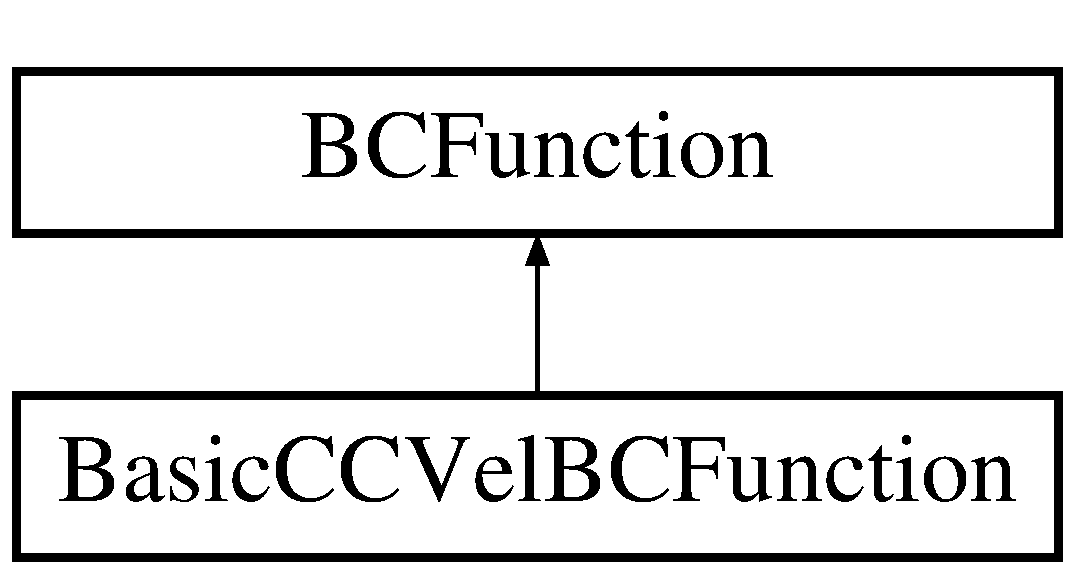
\includegraphics[height=2.000000cm]{class_basic_c_c_vel_b_c_function}
\end{center}
\end{figure}
\subsection*{Public Member Functions}
\begin{DoxyCompactItemize}
\item 
\hypertarget{class_basic_c_c_vel_b_c_function_a2aefce6b0178a7685f7e9a8870e06469}{\hyperlink{class_basic_c_c_vel_b_c_function_a2aefce6b0178a7685f7e9a8870e06469}{Basic\-C\-C\-Vel\-B\-C\-Function} ()}\label{class_basic_c_c_vel_b_c_function_a2aefce6b0178a7685f7e9a8870e06469}

\begin{DoxyCompactList}\small\item\em Default constructor. \end{DoxyCompactList}\item 
\hypertarget{class_basic_c_c_vel_b_c_function_af0169553178a9d0147b4b486b0d72984}{\hyperlink{class_basic_c_c_vel_b_c_function_af0169553178a9d0147b4b486b0d72984}{Basic\-C\-C\-Vel\-B\-C\-Function} (Real a\-\_\-bc\-Val, bool a\-\_\-is\-Homogeneous, bool a\-\_\-is\-Viscous, int a\-\_\-comp, const Interval \&a\-\_\-interval, \hyperlink{class_mushy_layer_params}{Mushy\-Layer\-Params} a\-\_\-params)}\label{class_basic_c_c_vel_b_c_function_af0169553178a9d0147b4b486b0d72984}

\begin{DoxyCompactList}\small\item\em Full constructor. \end{DoxyCompactList}\item 
\hypertarget{class_basic_c_c_vel_b_c_function_aaa772ec6372e133171a66d8d778a3cb7}{virtual void \hyperlink{class_basic_c_c_vel_b_c_function_aaa772ec6372e133171a66d8d778a3cb7}{operator()} (F\-Array\-Box \&a\-\_\-state, const Box \&a\-\_\-valid, const Problem\-Domain \&a\-\_\-domain, Real a\-\_\-dx, bool a\-\_\-homogeneous)}\label{class_basic_c_c_vel_b_c_function_aaa772ec6372e133171a66d8d778a3cb7}

\begin{DoxyCompactList}\small\item\em Apply B\-C. \end{DoxyCompactList}\end{DoxyCompactItemize}
\subsection*{Public Attributes}
\begin{DoxyCompactItemize}
\item 
\hypertarget{class_basic_c_c_vel_b_c_function_adeca967b84062f4242387b38461a8865}{int \hyperlink{class_basic_c_c_vel_b_c_function_adeca967b84062f4242387b38461a8865}{m\-\_\-comp}}\label{class_basic_c_c_vel_b_c_function_adeca967b84062f4242387b38461a8865}

\begin{DoxyCompactList}\small\item\em Component of velocity to apply B\-Cs to. \end{DoxyCompactList}\item 
\hypertarget{class_basic_c_c_vel_b_c_function_a252af4c47d5055d3b861f5e7353eec1e}{Real \hyperlink{class_basic_c_c_vel_b_c_function_a252af4c47d5055d3b861f5e7353eec1e}{m\-\_\-bc\-Val}}\label{class_basic_c_c_vel_b_c_function_a252af4c47d5055d3b861f5e7353eec1e}

\begin{DoxyCompactList}\small\item\em Currently unused. \end{DoxyCompactList}\item 
\hypertarget{class_basic_c_c_vel_b_c_function_ae7f9d35862d6f4d60b66a1cc2d471124}{bool \hyperlink{class_basic_c_c_vel_b_c_function_ae7f9d35862d6f4d60b66a1cc2d471124}{m\-\_\-is\-Homogeneous}}\label{class_basic_c_c_vel_b_c_function_ae7f9d35862d6f4d60b66a1cc2d471124}

\begin{DoxyCompactList}\small\item\em Always enforce homogeneous form of B\-Cs? \end{DoxyCompactList}\item 
\hypertarget{class_basic_c_c_vel_b_c_function_a58aac1d527fc1867d9dbff790b38609f}{bool \hyperlink{class_basic_c_c_vel_b_c_function_a58aac1d527fc1867d9dbff790b38609f}{m\-\_\-is\-Viscous}}\label{class_basic_c_c_vel_b_c_function_a58aac1d527fc1867d9dbff790b38609f}

\begin{DoxyCompactList}\small\item\em Is there non-\/zero viscosity? \end{DoxyCompactList}\item 
\hypertarget{class_basic_c_c_vel_b_c_function_a7697caeb1754d5cca737daff6dcb2445}{Interval \hyperlink{class_basic_c_c_vel_b_c_function_a7697caeb1754d5cca737daff6dcb2445}{m\-\_\-interval}}\label{class_basic_c_c_vel_b_c_function_a7697caeb1754d5cca737daff6dcb2445}

\begin{DoxyCompactList}\small\item\em Specifies where in a\-\_\-state we will find the component we should apply B\-Cs to. \end{DoxyCompactList}\item 
\hypertarget{class_basic_c_c_vel_b_c_function_aefbcd5a114ca8e72723790c20feb1466}{\hyperlink{class_mushy_layer_params}{Mushy\-Layer\-Params} \hyperlink{class_basic_c_c_vel_b_c_function_aefbcd5a114ca8e72723790c20feb1466}{m\-\_\-params}}\label{class_basic_c_c_vel_b_c_function_aefbcd5a114ca8e72723790c20feb1466}

\begin{DoxyCompactList}\small\item\em Physical parameters for the problem. \end{DoxyCompactList}\end{DoxyCompactItemize}


\subsection{Detailed Description}
Boundary condition for velocity (cell-\/centred) 

The documentation for this class was generated from the following file\-:\begin{DoxyCompactItemize}
\item 
/home/parkinsonjl/mushy-\/layer/\-B\-Cutil/Phys\-B\-C\-Util.\-cpp\end{DoxyCompactItemize}

\hypertarget{class_basic_e_c_vel_b_c_function}{\section{Basic\-E\-C\-Vel\-B\-C\-Function Class Reference}
\label{class_basic_e_c_vel_b_c_function}\index{Basic\-E\-C\-Vel\-B\-C\-Function@{Basic\-E\-C\-Vel\-B\-C\-Function}}
}


Boundary conditions for velocity (edge-\/centred)  


Inheritance diagram for Basic\-E\-C\-Vel\-B\-C\-Function\-:\begin{figure}[H]
\begin{center}
\leavevmode
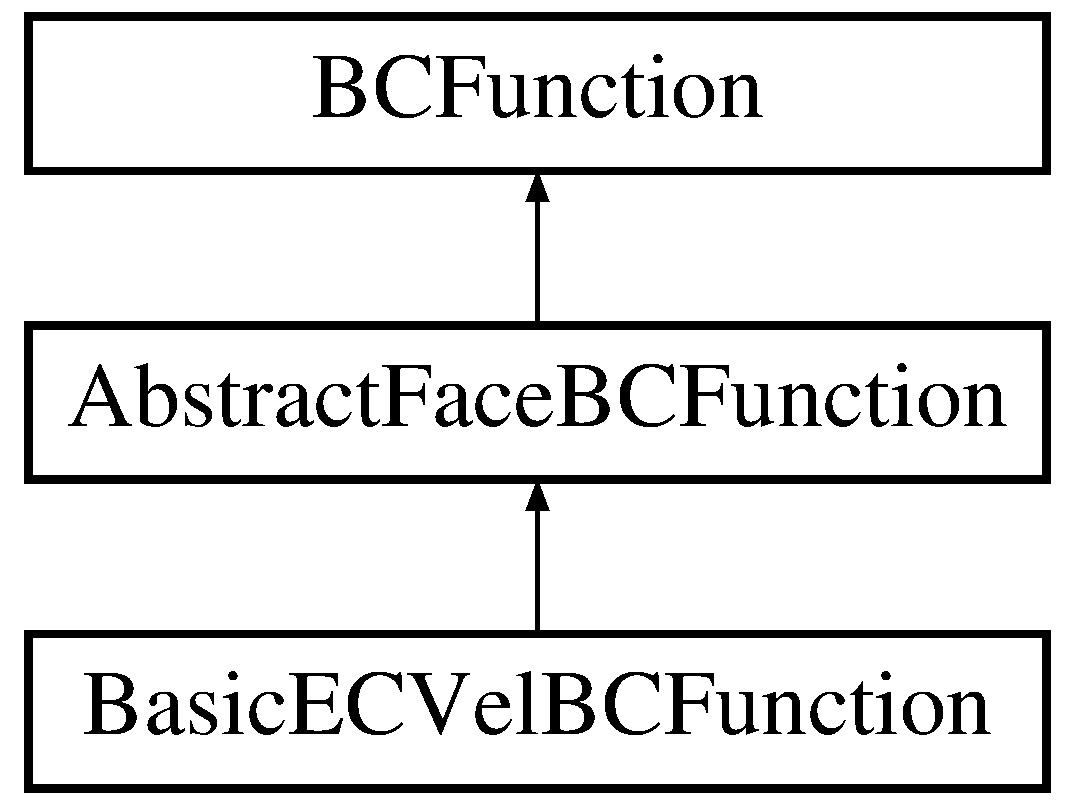
\includegraphics[height=3.000000cm]{class_basic_e_c_vel_b_c_function}
\end{center}
\end{figure}
\subsection*{Public Member Functions}
\begin{DoxyCompactItemize}
\item 
\hypertarget{class_basic_e_c_vel_b_c_function_a8ae38232cd83d5af7f7c2a2ca25bc714}{\hyperlink{class_basic_e_c_vel_b_c_function_a8ae38232cd83d5af7f7c2a2ca25bc714}{Basic\-E\-C\-Vel\-B\-C\-Function} (bool a\-\_\-is\-Homogeneous, bool a\-\_\-is\-Viscous, int a\-\_\-comp, const Interval \&a\-\_\-interval, \hyperlink{class_mushy_layer_params}{Mushy\-Layer\-Params} a\-\_\-params)}\label{class_basic_e_c_vel_b_c_function_a8ae38232cd83d5af7f7c2a2ca25bc714}

\begin{DoxyCompactList}\small\item\em Full constructor. \end{DoxyCompactList}\item 
\hypertarget{class_basic_e_c_vel_b_c_function_a4dc48ed586c036b77c1b85efbdfc4f92}{void \hyperlink{class_basic_e_c_vel_b_c_function_a4dc48ed586c036b77c1b85efbdfc4f92}{operator()} (F\-Array\-Box \&a\-\_\-state, const Box \&a\-\_\-valid, const Problem\-Domain \&a\-\_\-domain, Real a\-\_\-dx, bool a\-\_\-homogeneous)}\label{class_basic_e_c_vel_b_c_function_a4dc48ed586c036b77c1b85efbdfc4f92}

\begin{DoxyCompactList}\small\item\em Apply B\-C. \end{DoxyCompactList}\end{DoxyCompactItemize}
\subsection*{Public Attributes}
\begin{DoxyCompactItemize}
\item 
\hypertarget{class_basic_e_c_vel_b_c_function_aa1522389e5ac482263af7757e8a381e6}{bool \hyperlink{class_basic_e_c_vel_b_c_function_aa1522389e5ac482263af7757e8a381e6}{m\-\_\-is\-Viscous}}\label{class_basic_e_c_vel_b_c_function_aa1522389e5ac482263af7757e8a381e6}

\begin{DoxyCompactList}\small\item\em Is there non-\/zero viscosity? \end{DoxyCompactList}\item 
\hypertarget{class_basic_e_c_vel_b_c_function_aed09a1041c4354b17080f48ea887caa9}{Interval \hyperlink{class_basic_e_c_vel_b_c_function_aed09a1041c4354b17080f48ea887caa9}{m\-\_\-interval}}\label{class_basic_e_c_vel_b_c_function_aed09a1041c4354b17080f48ea887caa9}

\begin{DoxyCompactList}\small\item\em Currently unused. \end{DoxyCompactList}\end{DoxyCompactItemize}


\subsection{Detailed Description}
Boundary conditions for velocity (edge-\/centred) 

Sets specified boundary conditions for the velocity. For use on an edge-\/centred velocity, i.\-e. a Level\-Data$<$\-Flux\-Box$>$ 

The documentation for this class was generated from the following file\-:\begin{DoxyCompactItemize}
\item 
/home/parkinsonjl/mushy-\/layer/\-B\-Cutil/Phys\-B\-C\-Util.\-cpp\end{DoxyCompactItemize}

\hypertarget{class_basic_extrap_b_c_function}{\section{Basic\-Extrap\-B\-C\-Function Class Reference}
\label{class_basic_extrap_b_c_function}\index{Basic\-Extrap\-B\-C\-Function@{Basic\-Extrap\-B\-C\-Function}}
}


Apply extrapolation boundary condition on all sides.  


Inheritance diagram for Basic\-Extrap\-B\-C\-Function\-:\begin{figure}[H]
\begin{center}
\leavevmode
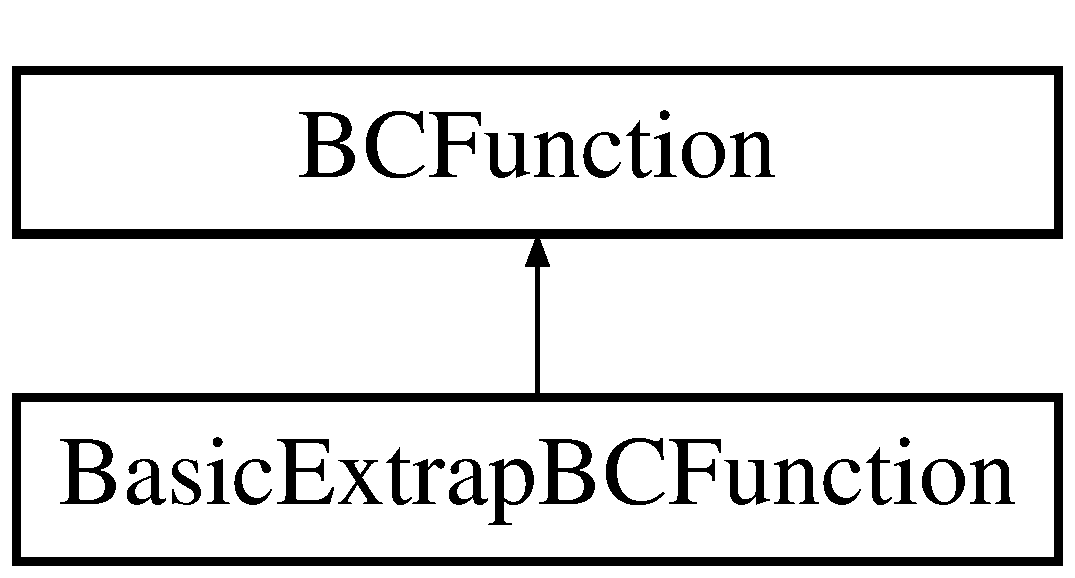
\includegraphics[height=2.000000cm]{class_basic_extrap_b_c_function}
\end{center}
\end{figure}
\subsection*{Public Member Functions}
\begin{DoxyCompactItemize}
\item 
\hypertarget{class_basic_extrap_b_c_function_a989fb8339fdf36db5afbce00a5ae98bc}{\hyperlink{class_basic_extrap_b_c_function_a989fb8339fdf36db5afbce00a5ae98bc}{Basic\-Extrap\-B\-C\-Function} ()}\label{class_basic_extrap_b_c_function_a989fb8339fdf36db5afbce00a5ae98bc}

\begin{DoxyCompactList}\small\item\em Default constructor. \end{DoxyCompactList}\item 
\hypertarget{class_basic_extrap_b_c_function_a96b6cfd3661ba2ccfa52c40683ccfe0a}{\hyperlink{class_basic_extrap_b_c_function_a96b6cfd3661ba2ccfa52c40683ccfe0a}{Basic\-Extrap\-B\-C\-Function} (bool a\-\_\-is\-Defined, \hyperlink{class_mushy_layer_params}{Mushy\-Layer\-Params} a\-\_\-params, int a\-\_\-ghost=1, int a\-\_\-comp=1)}\label{class_basic_extrap_b_c_function_a96b6cfd3661ba2ccfa52c40683ccfe0a}

\begin{DoxyCompactList}\small\item\em Full constructor. \end{DoxyCompactList}\item 
\hypertarget{class_basic_extrap_b_c_function_a68c6e7666355e178e8005b6e63473d19}{virtual void \hyperlink{class_basic_extrap_b_c_function_a68c6e7666355e178e8005b6e63473d19}{operator()} (F\-Array\-Box \&a\-\_\-state, const Box \&a\-\_\-valid, const Problem\-Domain \&a\-\_\-domain, Real a\-\_\-dx, bool a\-\_\-homogeneous)}\label{class_basic_extrap_b_c_function_a68c6e7666355e178e8005b6e63473d19}

\begin{DoxyCompactList}\small\item\em Apply B\-C. \end{DoxyCompactList}\end{DoxyCompactItemize}
\subsection*{Public Attributes}
\begin{DoxyCompactItemize}
\item 
\hypertarget{class_basic_extrap_b_c_function_afedbf88ca74b82464859f699b0634dea}{bool \hyperlink{class_basic_extrap_b_c_function_afedbf88ca74b82464859f699b0634dea}{m\-\_\-is\-Defined}}\label{class_basic_extrap_b_c_function_afedbf88ca74b82464859f699b0634dea}

\begin{DoxyCompactList}\small\item\em Is object defined? \end{DoxyCompactList}\item 
\hypertarget{class_basic_extrap_b_c_function_a746a5c4527d9c8ad96dcbbe2fbc834b0}{\hyperlink{class_mushy_layer_params}{Mushy\-Layer\-Params} \hyperlink{class_basic_extrap_b_c_function_a746a5c4527d9c8ad96dcbbe2fbc834b0}{m\-\_\-params}}\label{class_basic_extrap_b_c_function_a746a5c4527d9c8ad96dcbbe2fbc834b0}

\begin{DoxyCompactList}\small\item\em Physical parameters for the problem. \end{DoxyCompactList}\item 
\hypertarget{class_basic_extrap_b_c_function_a14b9554c8baea2a9b215272daac1f183}{int \hyperlink{class_basic_extrap_b_c_function_a14b9554c8baea2a9b215272daac1f183}{m\-\_\-ghost}}\label{class_basic_extrap_b_c_function_a14b9554c8baea2a9b215272daac1f183}

\begin{DoxyCompactList}\small\item\em Number of ghost cells to fill. \end{DoxyCompactList}\item 
\hypertarget{class_basic_extrap_b_c_function_a00c04067887286a621897ebb7778fcb1}{int \hyperlink{class_basic_extrap_b_c_function_a00c04067887286a621897ebb7778fcb1}{m\-\_\-comp}}\label{class_basic_extrap_b_c_function_a00c04067887286a621897ebb7778fcb1}

\begin{DoxyCompactList}\small\item\em Component of velocity to apply B\-Cs to. \end{DoxyCompactList}\end{DoxyCompactItemize}


\subsection{Detailed Description}
Apply extrapolation boundary condition on all sides. 

The documentation for this class was generated from the following file\-:\begin{DoxyCompactItemize}
\item 
/home/parkinsonjl/mushy-\/layer/\-B\-Cutil/Phys\-B\-C\-Util.\-cpp\end{DoxyCompactItemize}

\hypertarget{class_basic_extrap_interior_function}{\section{Basic\-Extrap\-Interior\-Function Class Reference}
\label{class_basic_extrap_interior_function}\index{Basic\-Extrap\-Interior\-Function@{Basic\-Extrap\-Interior\-Function}}
}


This class only fills cells on the interior of the domain!  


Inheritance diagram for Basic\-Extrap\-Interior\-Function\-:\begin{figure}[H]
\begin{center}
\leavevmode
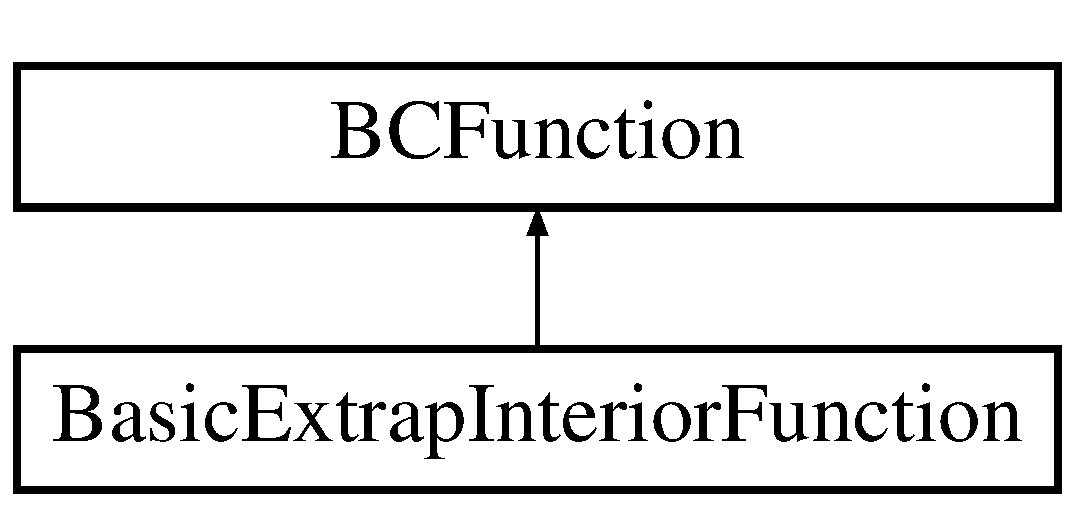
\includegraphics[height=2.000000cm]{class_basic_extrap_interior_function}
\end{center}
\end{figure}
\subsection*{Public Member Functions}
\begin{DoxyCompactItemize}
\item 
\hypertarget{class_basic_extrap_interior_function_a27c9cd01ac58476e1501d762d29a0b22}{\hyperlink{class_basic_extrap_interior_function_a27c9cd01ac58476e1501d762d29a0b22}{Basic\-Extrap\-Interior\-Function} ()}\label{class_basic_extrap_interior_function_a27c9cd01ac58476e1501d762d29a0b22}

\begin{DoxyCompactList}\small\item\em Default constructor. \end{DoxyCompactList}\item 
\hypertarget{class_basic_extrap_interior_function_a2b065fb8eac306deec75ae29512ea8fd}{\hyperlink{class_basic_extrap_interior_function_a2b065fb8eac306deec75ae29512ea8fd}{Basic\-Extrap\-Interior\-Function} (bool a\-\_\-is\-Defined, \hyperlink{class_mushy_layer_params}{Mushy\-Layer\-Params} a\-\_\-params, int a\-\_\-ghost)}\label{class_basic_extrap_interior_function_a2b065fb8eac306deec75ae29512ea8fd}

\begin{DoxyCompactList}\small\item\em Full constructor. \end{DoxyCompactList}\item 
\hypertarget{class_basic_extrap_interior_function_a67862d99ecbc2102bac335e28d7f39d4}{virtual void \hyperlink{class_basic_extrap_interior_function_a67862d99ecbc2102bac335e28d7f39d4}{operator()} (F\-Array\-Box \&a\-\_\-state, const Box \&a\-\_\-valid, const Problem\-Domain \&a\-\_\-domain, Real a\-\_\-dx, bool a\-\_\-homogeneous)}\label{class_basic_extrap_interior_function_a67862d99ecbc2102bac335e28d7f39d4}

\begin{DoxyCompactList}\small\item\em Apply B\-C. \end{DoxyCompactList}\end{DoxyCompactItemize}
\subsection*{Public Attributes}
\begin{DoxyCompactItemize}
\item 
\hypertarget{class_basic_extrap_interior_function_a5911f83345d9b3cb0ee298bc3c064e51}{bool \hyperlink{class_basic_extrap_interior_function_a5911f83345d9b3cb0ee298bc3c064e51}{m\-\_\-is\-Defined}}\label{class_basic_extrap_interior_function_a5911f83345d9b3cb0ee298bc3c064e51}

\begin{DoxyCompactList}\small\item\em Is object defined? \end{DoxyCompactList}\item 
\hypertarget{class_basic_extrap_interior_function_a2f965779be41bf4def8beb03fb734008}{\hyperlink{class_mushy_layer_params}{Mushy\-Layer\-Params} \hyperlink{class_basic_extrap_interior_function_a2f965779be41bf4def8beb03fb734008}{m\-\_\-params}}\label{class_basic_extrap_interior_function_a2f965779be41bf4def8beb03fb734008}

\begin{DoxyCompactList}\small\item\em Physical parameters for the problem. \end{DoxyCompactList}\item 
\hypertarget{class_basic_extrap_interior_function_a3b76f37832a33939ce6b5a83b73648e0}{int \hyperlink{class_basic_extrap_interior_function_a3b76f37832a33939ce6b5a83b73648e0}{m\-\_\-ghost}}\label{class_basic_extrap_interior_function_a3b76f37832a33939ce6b5a83b73648e0}

\begin{DoxyCompactList}\small\item\em Number of ghost cells to fill. \end{DoxyCompactList}\end{DoxyCompactItemize}


\subsection{Detailed Description}
This class only fills cells on the interior of the domain! 

The documentation for this class was generated from the following file\-:\begin{DoxyCompactItemize}
\item 
/home/parkinsonjl/mushy-\/layer/\-B\-Cutil/Phys\-B\-C\-Util.\-cpp\end{DoxyCompactItemize}

\hypertarget{class_basic_flux_extrap_b_c_function}{\section{Basic\-Flux\-Extrap\-B\-C\-Function Class Reference}
\label{class_basic_flux_extrap_b_c_function}\index{Basic\-Flux\-Extrap\-B\-C\-Function@{Basic\-Flux\-Extrap\-B\-C\-Function}}
}


Apply extrapolation B\-Cs to a flux component.  


Inheritance diagram for Basic\-Flux\-Extrap\-B\-C\-Function\-:\begin{figure}[H]
\begin{center}
\leavevmode
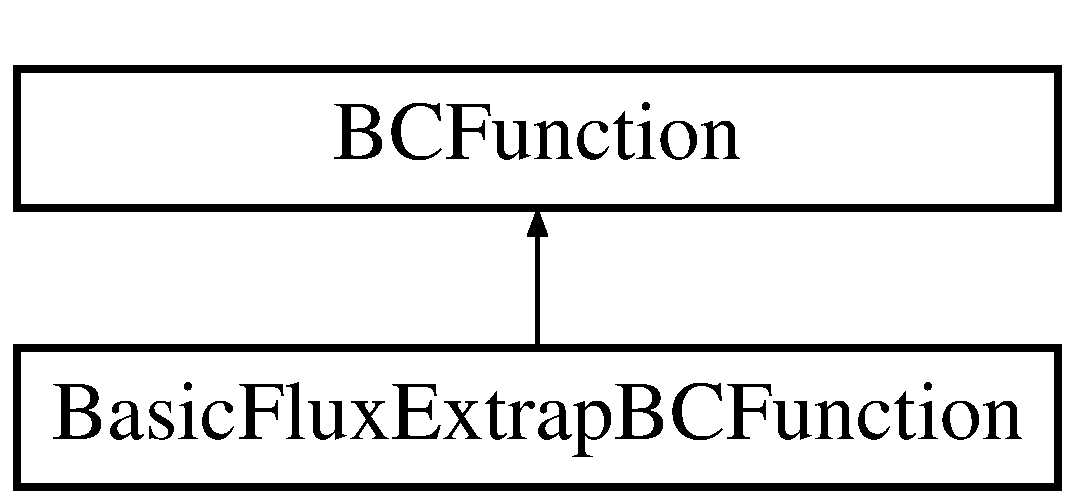
\includegraphics[height=2.000000cm]{class_basic_flux_extrap_b_c_function}
\end{center}
\end{figure}
\subsection*{Public Member Functions}
\begin{DoxyCompactItemize}
\item 
\hypertarget{class_basic_flux_extrap_b_c_function_a0f3d312b4ee41771e6e48b8bd4f17469}{\hyperlink{class_basic_flux_extrap_b_c_function_a0f3d312b4ee41771e6e48b8bd4f17469}{Basic\-Flux\-Extrap\-B\-C\-Function} (int a\-\_\-comp)}\label{class_basic_flux_extrap_b_c_function_a0f3d312b4ee41771e6e48b8bd4f17469}

\begin{DoxyCompactList}\small\item\em Full constructor. \end{DoxyCompactList}\item 
\hypertarget{class_basic_flux_extrap_b_c_function_abe5db40b5f849d39e06b44376d0b6bdf}{virtual void \hyperlink{class_basic_flux_extrap_b_c_function_abe5db40b5f849d39e06b44376d0b6bdf}{operator()} (F\-Array\-Box \&a\-\_\-state, const Box \&a\-\_\-valid, const Problem\-Domain \&a\-\_\-domain, Real a\-\_\-dx, bool a\-\_\-homogeneous)}\label{class_basic_flux_extrap_b_c_function_abe5db40b5f849d39e06b44376d0b6bdf}

\begin{DoxyCompactList}\small\item\em Apply B\-C. \end{DoxyCompactList}\end{DoxyCompactItemize}
\subsection*{Public Attributes}
\begin{DoxyCompactItemize}
\item 
\hypertarget{class_basic_flux_extrap_b_c_function_ad57cef41aad080d3997f5ecebd2936e1}{int \hyperlink{class_basic_flux_extrap_b_c_function_ad57cef41aad080d3997f5ecebd2936e1}{m\-\_\-comp}}\label{class_basic_flux_extrap_b_c_function_ad57cef41aad080d3997f5ecebd2936e1}

\begin{DoxyCompactList}\small\item\em Component of velocity to apply B\-Cs to. \end{DoxyCompactList}\end{DoxyCompactItemize}


\subsection{Detailed Description}
Apply extrapolation B\-Cs to a flux component. 

Extrapolation B\-Cs for the specified component of a flux box. 

The documentation for this class was generated from the following file\-:\begin{DoxyCompactItemize}
\item 
/home/parkinsonjl/mushy-\/layer/\-B\-Cutil/Phys\-B\-C\-Util.\-cpp\end{DoxyCompactItemize}

\hypertarget{class_basic_grad_pressure_b_c_function}{\section{Basic\-Grad\-Pressure\-B\-C\-Function Class Reference}
\label{class_basic_grad_pressure_b_c_function}\index{Basic\-Grad\-Pressure\-B\-C\-Function@{Basic\-Grad\-Pressure\-B\-C\-Function}}
}


Boundary condition for the pressure gradient.  


Inheritance diagram for Basic\-Grad\-Pressure\-B\-C\-Function\-:\begin{figure}[H]
\begin{center}
\leavevmode
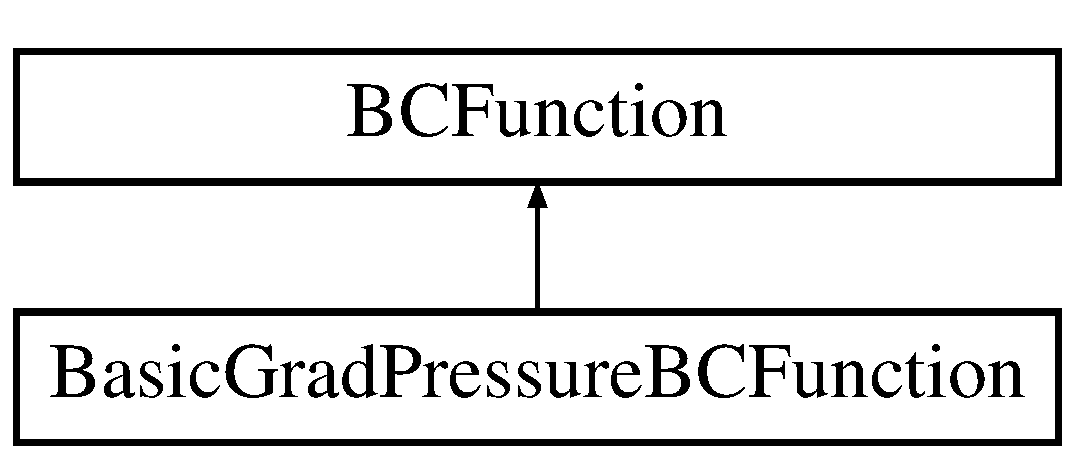
\includegraphics[height=2.000000cm]{class_basic_grad_pressure_b_c_function}
\end{center}
\end{figure}
\subsection*{Public Member Functions}
\begin{DoxyCompactItemize}
\item 
\hypertarget{class_basic_grad_pressure_b_c_function_a26372a752dd51acbaa659039b70980e4}{\hyperlink{class_basic_grad_pressure_b_c_function_a26372a752dd51acbaa659039b70980e4}{Basic\-Grad\-Pressure\-B\-C\-Function} ()}\label{class_basic_grad_pressure_b_c_function_a26372a752dd51acbaa659039b70980e4}

\begin{DoxyCompactList}\small\item\em Default constructor. \end{DoxyCompactList}\item 
\hypertarget{class_basic_grad_pressure_b_c_function_ae6c3e1cbb5fa5fc028d678ab12f133e6}{\hyperlink{class_basic_grad_pressure_b_c_function_ae6c3e1cbb5fa5fc028d678ab12f133e6}{Basic\-Grad\-Pressure\-B\-C\-Function} (bool a\-\_\-is\-Defined, \hyperlink{class_mushy_layer_params}{Mushy\-Layer\-Params} a\-\_\-params)}\label{class_basic_grad_pressure_b_c_function_ae6c3e1cbb5fa5fc028d678ab12f133e6}

\begin{DoxyCompactList}\small\item\em Full constructor. \end{DoxyCompactList}\item 
\hypertarget{class_basic_grad_pressure_b_c_function_a96a8f342fb3f7cfffe2998ec22f07bc9}{virtual void \hyperlink{class_basic_grad_pressure_b_c_function_a96a8f342fb3f7cfffe2998ec22f07bc9}{operator()} (F\-Array\-Box \&a\-\_\-state, const Box \&a\-\_\-valid, const Problem\-Domain \&a\-\_\-domain, Real a\-\_\-dx, bool a\-\_\-homogeneous)}\label{class_basic_grad_pressure_b_c_function_a96a8f342fb3f7cfffe2998ec22f07bc9}

\begin{DoxyCompactList}\small\item\em Apply B\-C. \end{DoxyCompactList}\end{DoxyCompactItemize}
\subsection*{Public Attributes}
\begin{DoxyCompactItemize}
\item 
\hypertarget{class_basic_grad_pressure_b_c_function_ab06c724ad26290b8b8fd7fb332890d0f}{bool \hyperlink{class_basic_grad_pressure_b_c_function_ab06c724ad26290b8b8fd7fb332890d0f}{m\-\_\-is\-Defined}}\label{class_basic_grad_pressure_b_c_function_ab06c724ad26290b8b8fd7fb332890d0f}

\begin{DoxyCompactList}\small\item\em Is object defined? \end{DoxyCompactList}\item 
\hypertarget{class_basic_grad_pressure_b_c_function_a803f06865c3dcb81d220f4410b569113}{\hyperlink{class_mushy_layer_params}{Mushy\-Layer\-Params} \hyperlink{class_basic_grad_pressure_b_c_function_a803f06865c3dcb81d220f4410b569113}{m\-\_\-params}}\label{class_basic_grad_pressure_b_c_function_a803f06865c3dcb81d220f4410b569113}

\begin{DoxyCompactList}\small\item\em Physical parameters for the problem. \end{DoxyCompactList}\end{DoxyCompactItemize}


\subsection{Detailed Description}
Boundary condition for the pressure gradient. 

Extrapolation on all sides 

The documentation for this class was generated from the following file\-:\begin{DoxyCompactItemize}
\item 
/home/parkinsonjl/mushy-\/layer/\-B\-Cutil/Phys\-B\-C\-Util.\-cpp\end{DoxyCompactItemize}

\hypertarget{class_basic_porosity_permeability_b_c_function}{\section{Basic\-Porosity\-Permeability\-B\-C\-Function Class Reference}
\label{class_basic_porosity_permeability_b_c_function}\index{Basic\-Porosity\-Permeability\-B\-C\-Function@{Basic\-Porosity\-Permeability\-B\-C\-Function}}
}


Boundary conditions for $\Pi$ (permeability)  


Inheritance diagram for Basic\-Porosity\-Permeability\-B\-C\-Function\-:\begin{figure}[H]
\begin{center}
\leavevmode
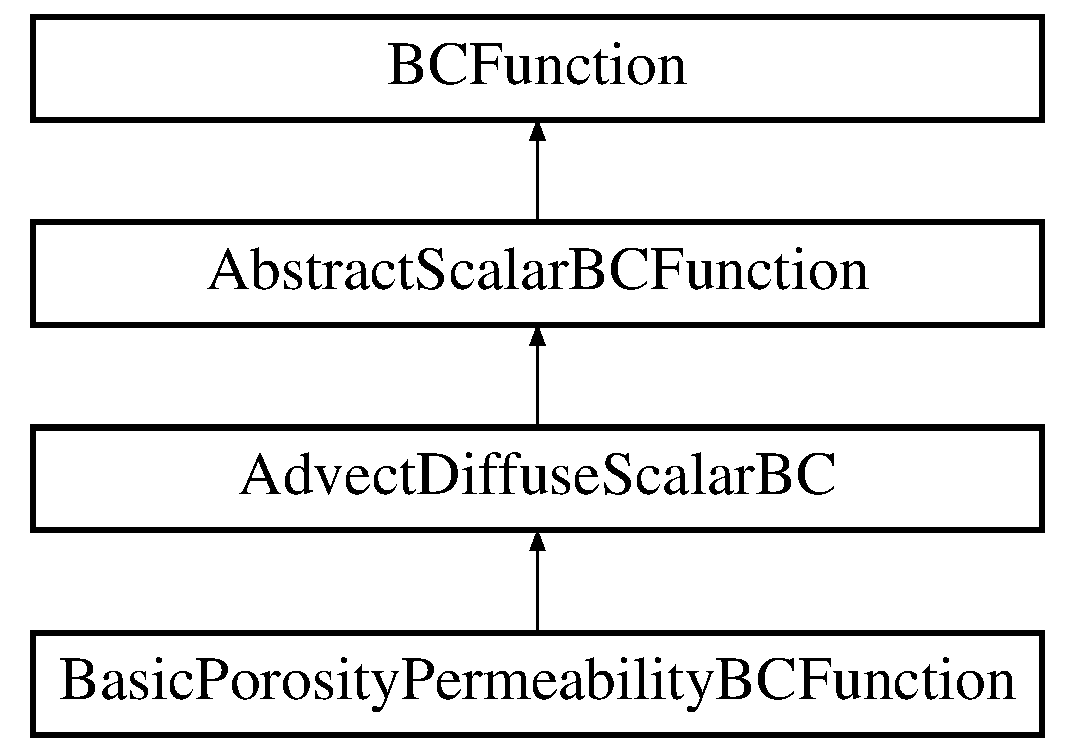
\includegraphics[height=4.000000cm]{class_basic_porosity_permeability_b_c_function}
\end{center}
\end{figure}
\subsection*{Public Member Functions}
\begin{DoxyCompactItemize}
\item 
\hypertarget{class_basic_porosity_permeability_b_c_function_a0b9bf045ea7a47fee8064ca8a0437eee}{{\bfseries Basic\-Porosity\-Permeability\-B\-C\-Function} (bool a\-\_\-is\-Defined, \hyperlink{class_mushy_layer_params}{Mushy\-Layer\-Params} a\-\_\-params, bool a\-\_\-homogeneous, Level\-Data$<$ Flux\-Box $>$ $\ast$a\-\_\-adv\-Vel, Real a\-\_\-dx, Vector$<$ Real $>$ a\-\_\-plume\-Val, Interval intvl, Vector$<$ Vector$<$ int $>$ $>$ \&a\-\_\-custom\-Lo\-B\-C, Vector$<$ Vector$<$ int $>$ $>$ \&a\-\_\-custom\-Hi\-B\-C, Vector$<$ Vector$<$ Real $>$ $>$ \&a\-\_\-custom\-Lo\-B\-C\-Val, Vector$<$ Vector$<$ Real $>$ $>$ \&a\-\_\-custom\-Hi\-B\-C\-Val)}\label{class_basic_porosity_permeability_b_c_function_a0b9bf045ea7a47fee8064ca8a0437eee}

\item 
void \hyperlink{class_basic_porosity_permeability_b_c_function_a436d10317f86cbf27980f1b3a694386a}{operator()} (F\-Array\-Box \&a\-\_\-state, const Box \&a\-\_\-valid, const Problem\-Domain \&a\-\_\-domain, Real a\-\_\-dx, bool a\-\_\-homogeneous)
\begin{DoxyCompactList}\small\item\em Apply B\-C. \end{DoxyCompactList}\end{DoxyCompactItemize}
\subsection*{Additional Inherited Members}


\subsection{Detailed Description}
Boundary conditions for $\Pi$ (permeability) 

\subsection{Member Function Documentation}
\hypertarget{class_basic_porosity_permeability_b_c_function_a436d10317f86cbf27980f1b3a694386a}{\index{Basic\-Porosity\-Permeability\-B\-C\-Function@{Basic\-Porosity\-Permeability\-B\-C\-Function}!operator()@{operator()}}
\index{operator()@{operator()}!BasicPorosityPermeabilityBCFunction@{Basic\-Porosity\-Permeability\-B\-C\-Function}}
\subsubsection[{operator()}]{\setlength{\rightskip}{0pt plus 5cm}void Basic\-Porosity\-Permeability\-B\-C\-Function\-::operator() (
\begin{DoxyParamCaption}
\item[{F\-Array\-Box \&}]{a\-\_\-state, }
\item[{const Box \&}]{a\-\_\-valid, }
\item[{const Problem\-Domain \&}]{a\-\_\-domain, }
\item[{Real}]{a\-\_\-dx, }
\item[{bool}]{a\-\_\-homogeneous}
\end{DoxyParamCaption}
)\hspace{0.3cm}{\ttfamily [inline]}, {\ttfamily [virtual]}}}\label{class_basic_porosity_permeability_b_c_function_a436d10317f86cbf27980f1b3a694386a}


Apply B\-C. 

assuming we only have one component to fill here 

Reimplemented from \hyperlink{class_advect_diffuse_scalar_b_c_ab55b1f2a27a3ff1ecda0d56acdbf0d77}{Advect\-Diffuse\-Scalar\-B\-C}.



The documentation for this class was generated from the following file\-:\begin{DoxyCompactItemize}
\item 
/home/parkinsonjl/mushy-\/layer/\-B\-Cutil/Phys\-B\-C\-Util.\-cpp\end{DoxyCompactItemize}

\hypertarget{class_basic_porosity_permeability_face_b_c_function}{\section{Basic\-Porosity\-Permeability\-Face\-B\-C\-Function Class Reference}
\label{class_basic_porosity_permeability_face_b_c_function}\index{Basic\-Porosity\-Permeability\-Face\-B\-C\-Function@{Basic\-Porosity\-Permeability\-Face\-B\-C\-Function}}
}


B\-C object for edge centered porosity.  


Inheritance diagram for Basic\-Porosity\-Permeability\-Face\-B\-C\-Function\-:\begin{figure}[H]
\begin{center}
\leavevmode
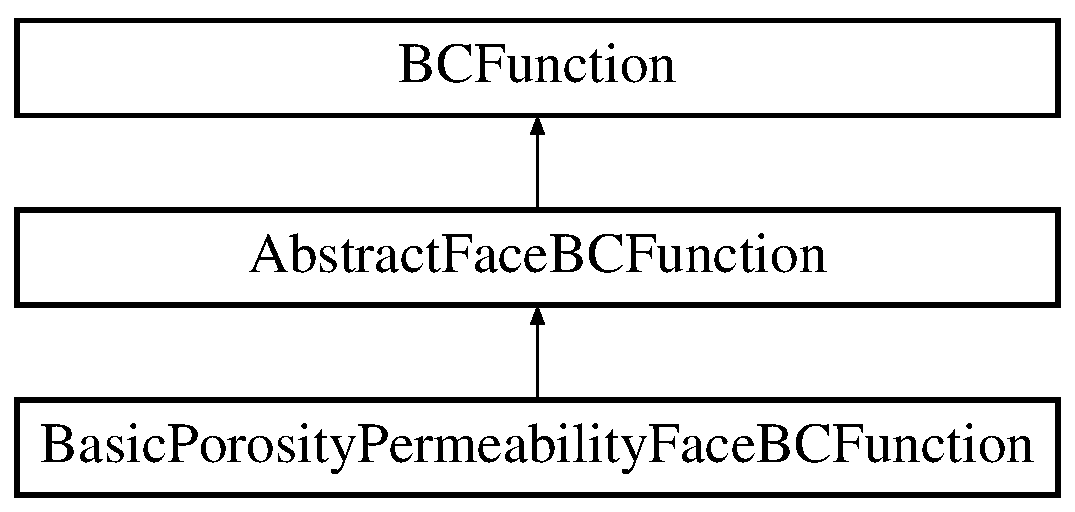
\includegraphics[height=3.000000cm]{class_basic_porosity_permeability_face_b_c_function}
\end{center}
\end{figure}
\subsection*{Public Member Functions}
\begin{DoxyCompactItemize}
\item 
\hypertarget{class_basic_porosity_permeability_face_b_c_function_a9c4f07215d310756b2cb65d57566c10c}{\hyperlink{class_basic_porosity_permeability_face_b_c_function_a9c4f07215d310756b2cb65d57566c10c}{Basic\-Porosity\-Permeability\-Face\-B\-C\-Function} (bool a\-\_\-is\-Homogeneous, int a\-\_\-comp, \hyperlink{class_mushy_layer_params}{Mushy\-Layer\-Params} a\-\_\-params, Real a\-\_\-plume\-Val, Vector$<$ Vector$<$ int $>$ $>$ a\-\_\-bc\-Type\-Lo, Vector$<$ Vector$<$ int $>$ $>$ a\-\_\-bc\-Type\-Hi, Vector$<$ Vector$<$ Real $>$ $>$ a\-\_\-bc\-Val\-Lo, Vector$<$ Vector$<$ Real $>$ $>$ a\-\_\-bc\-Val\-Hi)}\label{class_basic_porosity_permeability_face_b_c_function_a9c4f07215d310756b2cb65d57566c10c}

\begin{DoxyCompactList}\small\item\em Full constructor. \end{DoxyCompactList}\item 
\hypertarget{class_basic_porosity_permeability_face_b_c_function_a1acbb0ff29e6fe27f3a0907c611bddf2}{void \hyperlink{class_basic_porosity_permeability_face_b_c_function_a1acbb0ff29e6fe27f3a0907c611bddf2}{operator()} (F\-Array\-Box \&a\-\_\-state, const Box \&a\-\_\-valid, const Problem\-Domain \&a\-\_\-domain, Real a\-\_\-dx, bool a\-\_\-homogeneous)}\label{class_basic_porosity_permeability_face_b_c_function_a1acbb0ff29e6fe27f3a0907c611bddf2}

\begin{DoxyCompactList}\small\item\em Apply B\-C. \end{DoxyCompactList}\end{DoxyCompactItemize}
\subsection*{Public Attributes}
\begin{DoxyCompactItemize}
\item 
\hypertarget{class_basic_porosity_permeability_face_b_c_function_aa1d072b0f7a83cee89f8c74800724f2f}{Real {\bfseries m\-\_\-plume\-Val}}\label{class_basic_porosity_permeability_face_b_c_function_aa1d072b0f7a83cee89f8c74800724f2f}

\item 
\hypertarget{class_basic_porosity_permeability_face_b_c_function_adf25634e67df48830f18ddd5c2aab692}{Vector$<$ Vector$<$ int $>$ $>$ {\bfseries m\-\_\-bc\-Type\-Lo}}\label{class_basic_porosity_permeability_face_b_c_function_adf25634e67df48830f18ddd5c2aab692}

\item 
\hypertarget{class_basic_porosity_permeability_face_b_c_function_a14bc35227bde0f362318c3089918d728}{Vector$<$ Vector$<$ int $>$ $>$ {\bfseries m\-\_\-bc\-Type\-Hi}}\label{class_basic_porosity_permeability_face_b_c_function_a14bc35227bde0f362318c3089918d728}

\item 
\hypertarget{class_basic_porosity_permeability_face_b_c_function_afb2fb410e5dbcd33748fd5085c2fb0d4}{Vector$<$ Vector$<$ Real $>$ $>$ {\bfseries m\-\_\-bc\-Val\-Lo}}\label{class_basic_porosity_permeability_face_b_c_function_afb2fb410e5dbcd33748fd5085c2fb0d4}

\item 
\hypertarget{class_basic_porosity_permeability_face_b_c_function_ae15db449a406cd36b5b2306eb5ef8aeb}{Vector$<$ Vector$<$ Real $>$ $>$ {\bfseries m\-\_\-bc\-Val\-Hi}}\label{class_basic_porosity_permeability_face_b_c_function_ae15db449a406cd36b5b2306eb5ef8aeb}

\end{DoxyCompactItemize}


\subsection{Detailed Description}
B\-C object for edge centered porosity. 

The documentation for this class was generated from the following file\-:\begin{DoxyCompactItemize}
\item 
/home/parkinsonjl/mushy-\/layer/\-B\-Cutil/Phys\-B\-C\-Util.\-cpp\end{DoxyCompactItemize}

\hypertarget{class_basic_pressure_b_c_function}{\section{Basic\-Pressure\-B\-C\-Function Class Reference}
\label{class_basic_pressure_b_c_function}\index{Basic\-Pressure\-B\-C\-Function@{Basic\-Pressure\-B\-C\-Function}}
}


Boundary conditions for $P$ (pressure)  


Inheritance diagram for Basic\-Pressure\-B\-C\-Function\-:\begin{figure}[H]
\begin{center}
\leavevmode
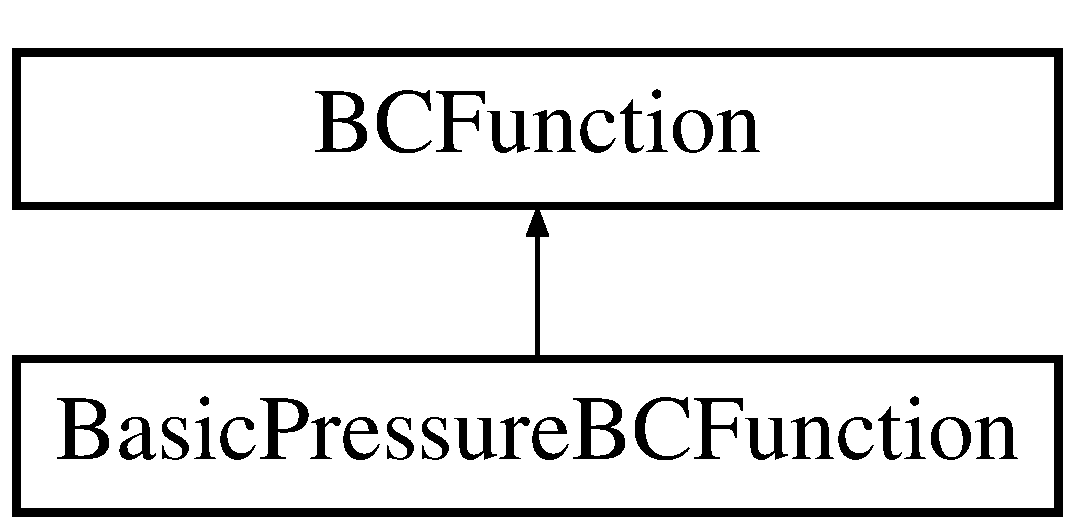
\includegraphics[height=2.000000cm]{class_basic_pressure_b_c_function}
\end{center}
\end{figure}
\subsection*{Public Member Functions}
\begin{DoxyCompactItemize}
\item 
\hypertarget{class_basic_pressure_b_c_function_aa7dc8b5320567833c200b65b668a5302}{\hyperlink{class_basic_pressure_b_c_function_aa7dc8b5320567833c200b65b668a5302}{Basic\-Pressure\-B\-C\-Function} ()}\label{class_basic_pressure_b_c_function_aa7dc8b5320567833c200b65b668a5302}

\begin{DoxyCompactList}\small\item\em Default constructor. \end{DoxyCompactList}\item 
\hypertarget{class_basic_pressure_b_c_function_aff0d91afdc797c0d253a747cd34e123d}{\hyperlink{class_basic_pressure_b_c_function_aff0d91afdc797c0d253a747cd34e123d}{Basic\-Pressure\-B\-C\-Function} (bool a\-\_\-is\-Defined, bool a\-\_\-is\-Homogeneous, \hyperlink{class_mushy_layer_params}{Mushy\-Layer\-Params} a\-\_\-params, Vector$<$ Ref\-Counted\-Ptr$<$ Level\-Data$<$ F\-Array\-Box $>$ $>$ $>$ a\-\_\-theta)}\label{class_basic_pressure_b_c_function_aff0d91afdc797c0d253a747cd34e123d}

\begin{DoxyCompactList}\small\item\em Full constructor. \end{DoxyCompactList}\item 
\hypertarget{class_basic_pressure_b_c_function_a944fde5ba556caf5f590972b60926fd2}{virtual void \hyperlink{class_basic_pressure_b_c_function_a944fde5ba556caf5f590972b60926fd2}{operator()} (F\-Array\-Box \&a\-\_\-state, const Box \&a\-\_\-valid, const Problem\-Domain \&a\-\_\-domain, Real a\-\_\-dx, bool a\-\_\-homogeneous)}\label{class_basic_pressure_b_c_function_a944fde5ba556caf5f590972b60926fd2}

\begin{DoxyCompactList}\small\item\em Apply B\-C. \end{DoxyCompactList}\end{DoxyCompactItemize}
\subsection*{Public Attributes}
\begin{DoxyCompactItemize}
\item 
\hypertarget{class_basic_pressure_b_c_function_a43356f3f0a9b5c53eb640704fa31164f}{bool \hyperlink{class_basic_pressure_b_c_function_a43356f3f0a9b5c53eb640704fa31164f}{m\-\_\-is\-Defined}}\label{class_basic_pressure_b_c_function_a43356f3f0a9b5c53eb640704fa31164f}

\begin{DoxyCompactList}\small\item\em Is object defined? \end{DoxyCompactList}\item 
\hypertarget{class_basic_pressure_b_c_function_aaa9abdedf2ccc38350fa36510a738f53}{bool \hyperlink{class_basic_pressure_b_c_function_aaa9abdedf2ccc38350fa36510a738f53}{m\-\_\-is\-Homogeneous}}\label{class_basic_pressure_b_c_function_aaa9abdedf2ccc38350fa36510a738f53}

\begin{DoxyCompactList}\small\item\em Always enforce homogeneous form of B\-Cs? \end{DoxyCompactList}\item 
\hypertarget{class_basic_pressure_b_c_function_a6330db574ca42615d78c4ddac98e4ccd}{\hyperlink{class_mushy_layer_params}{Mushy\-Layer\-Params} \hyperlink{class_basic_pressure_b_c_function_a6330db574ca42615d78c4ddac98e4ccd}{m\-\_\-params}}\label{class_basic_pressure_b_c_function_a6330db574ca42615d78c4ddac98e4ccd}

\begin{DoxyCompactList}\small\item\em Physical parameters for the problem. \end{DoxyCompactList}\item 
\hypertarget{class_basic_pressure_b_c_function_a232e0c7e4b9e41dd05a0cc4d33ac2920}{Vector$<$ Ref\-Counted\-Ptr\\*
$<$ Level\-Data$<$ F\-Array\-Box $>$ $>$ $>$ \hyperlink{class_basic_pressure_b_c_function_a232e0c7e4b9e41dd05a0cc4d33ac2920}{m\-\_\-theta}}\label{class_basic_pressure_b_c_function_a232e0c7e4b9e41dd05a0cc4d33ac2920}

\begin{DoxyCompactList}\small\item\em Temperature, for determining B\-Cs. \end{DoxyCompactList}\end{DoxyCompactItemize}


\subsection{Detailed Description}
Boundary conditions for $P$ (pressure) 

The documentation for this class was generated from the following file\-:\begin{DoxyCompactItemize}
\item 
/home/parkinsonjl/mushy-\/layer/\-B\-Cutil/Phys\-B\-C\-Util.\-cpp\end{DoxyCompactItemize}

\hypertarget{class_basic_pressure_b_c_function_subcycled}{\section{Basic\-Pressure\-B\-C\-Function\-Subcycled Class Reference}
\label{class_basic_pressure_b_c_function_subcycled}\index{Basic\-Pressure\-B\-C\-Function\-Subcycled@{Basic\-Pressure\-B\-C\-Function\-Subcycled}}
}


Boundary conditions for pressure $P$ (subcycled version)  


Inheritance diagram for Basic\-Pressure\-B\-C\-Function\-Subcycled\-:\begin{figure}[H]
\begin{center}
\leavevmode
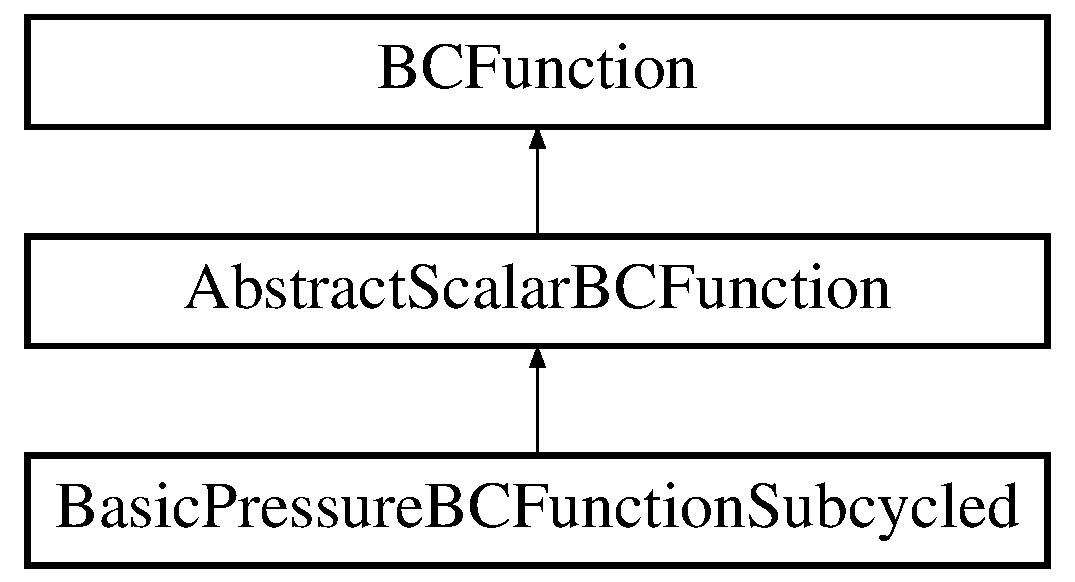
\includegraphics[height=3.000000cm]{class_basic_pressure_b_c_function_subcycled}
\end{center}
\end{figure}
\subsection*{Public Member Functions}
\begin{DoxyCompactItemize}
\item 
\hypertarget{class_basic_pressure_b_c_function_subcycled_a6a5170b9ac2de09c1a41a48dd7bb53cd}{{\bfseries Basic\-Pressure\-B\-C\-Function\-Subcycled} (bool a\-\_\-is\-Defined, \hyperlink{class_mushy_layer_params}{Mushy\-Layer\-Params} a\-\_\-params, bool a\-\_\-homogeneous, Level\-Data$<$ Flux\-Box $>$ $\ast$a\-\_\-adv\-Vel, Real a\-\_\-dx)}\label{class_basic_pressure_b_c_function_subcycled_a6a5170b9ac2de09c1a41a48dd7bb53cd}

\item 
\hypertarget{class_basic_pressure_b_c_function_subcycled_a11485aa5383fdd9b183da7905d852276}{void \hyperlink{class_basic_pressure_b_c_function_subcycled_a11485aa5383fdd9b183da7905d852276}{operator()} (F\-Array\-Box \&a\-\_\-state, const Box \&a\-\_\-valid, const Problem\-Domain \&a\-\_\-domain, Real a\-\_\-dx, bool a\-\_\-homogeneous)}\label{class_basic_pressure_b_c_function_subcycled_a11485aa5383fdd9b183da7905d852276}

\begin{DoxyCompactList}\small\item\em Apply B\-C. \end{DoxyCompactList}\end{DoxyCompactItemize}
\subsection*{Additional Inherited Members}


\subsection{Detailed Description}
Boundary conditions for pressure $P$ (subcycled version) 

The documentation for this class was generated from the following file\-:\begin{DoxyCompactItemize}
\item 
/home/parkinsonjl/mushy-\/layer/\-B\-Cutil/Phys\-B\-C\-Util.\-cpp\end{DoxyCompactItemize}

\hypertarget{class_basic_reflux_corr_b_c_function}{\section{Basic\-Reflux\-Corr\-B\-C\-Function Class Reference}
\label{class_basic_reflux_corr_b_c_function}\index{Basic\-Reflux\-Corr\-B\-C\-Function@{Basic\-Reflux\-Corr\-B\-C\-Function}}
}


Boundary condition for reflux correction.  


Inheritance diagram for Basic\-Reflux\-Corr\-B\-C\-Function\-:\begin{figure}[H]
\begin{center}
\leavevmode
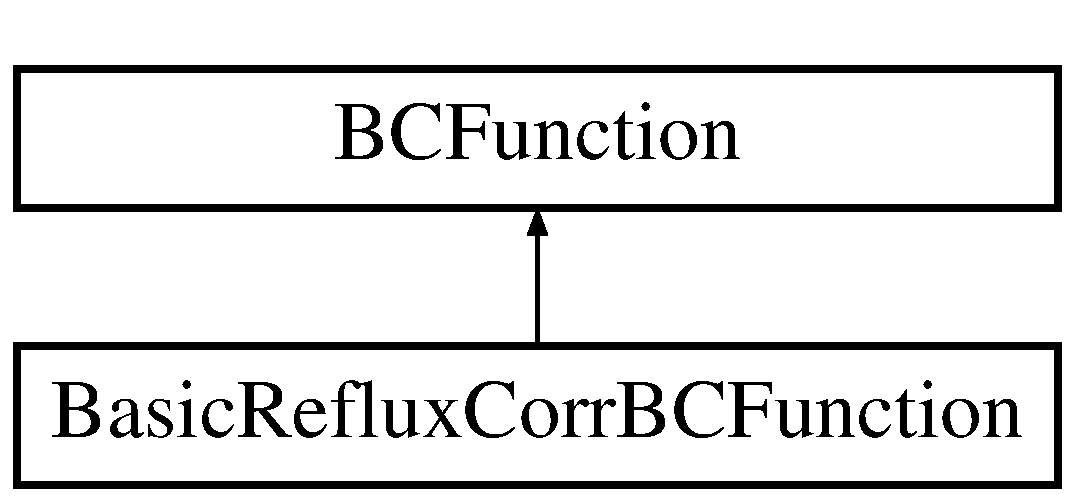
\includegraphics[height=2.000000cm]{class_basic_reflux_corr_b_c_function}
\end{center}
\end{figure}
\subsection*{Public Member Functions}
\begin{DoxyCompactItemize}
\item 
\hypertarget{class_basic_reflux_corr_b_c_function_a891b9aa97bcbdac51b3f0170c0608255}{\hyperlink{class_basic_reflux_corr_b_c_function_a891b9aa97bcbdac51b3f0170c0608255}{Basic\-Reflux\-Corr\-B\-C\-Function} ()}\label{class_basic_reflux_corr_b_c_function_a891b9aa97bcbdac51b3f0170c0608255}

\begin{DoxyCompactList}\small\item\em Default constructor. \end{DoxyCompactList}\item 
\hypertarget{class_basic_reflux_corr_b_c_function_a785a5780cdf367b9e945f8c991115b9d}{\hyperlink{class_basic_reflux_corr_b_c_function_a785a5780cdf367b9e945f8c991115b9d}{Basic\-Reflux\-Corr\-B\-C\-Function} (bool a\-\_\-is\-Defined, \hyperlink{class_mushy_layer_params}{Mushy\-Layer\-Params} a\-\_\-params)}\label{class_basic_reflux_corr_b_c_function_a785a5780cdf367b9e945f8c991115b9d}

\begin{DoxyCompactList}\small\item\em Full constructor. \end{DoxyCompactList}\item 
\hypertarget{class_basic_reflux_corr_b_c_function_a2c253616dd672bae591b3686d65270f3}{virtual void \hyperlink{class_basic_reflux_corr_b_c_function_a2c253616dd672bae591b3686d65270f3}{operator()} (F\-Array\-Box \&a\-\_\-state, const Box \&a\-\_\-valid, const Problem\-Domain \&a\-\_\-domain, Real a\-\_\-dx, bool a\-\_\-homogeneous)}\label{class_basic_reflux_corr_b_c_function_a2c253616dd672bae591b3686d65270f3}

\begin{DoxyCompactList}\small\item\em Apply B\-C. \end{DoxyCompactList}\end{DoxyCompactItemize}
\subsection*{Public Attributes}
\begin{DoxyCompactItemize}
\item 
\hypertarget{class_basic_reflux_corr_b_c_function_a667eac94d48b9867f55f03c949718081}{bool \hyperlink{class_basic_reflux_corr_b_c_function_a667eac94d48b9867f55f03c949718081}{m\-\_\-is\-Defined}}\label{class_basic_reflux_corr_b_c_function_a667eac94d48b9867f55f03c949718081}

\begin{DoxyCompactList}\small\item\em Is object defined? \end{DoxyCompactList}\item 
\hypertarget{class_basic_reflux_corr_b_c_function_a995e4e848ecd97309a1fcd549a1a969b}{\hyperlink{class_mushy_layer_params}{Mushy\-Layer\-Params} \hyperlink{class_basic_reflux_corr_b_c_function_a995e4e848ecd97309a1fcd549a1a969b}{m\-\_\-params}}\label{class_basic_reflux_corr_b_c_function_a995e4e848ecd97309a1fcd549a1a969b}

\begin{DoxyCompactList}\small\item\em Physical parameters for the problem. \end{DoxyCompactList}\end{DoxyCompactItemize}


\subsection{Detailed Description}
Boundary condition for reflux correction. 

Sets correction = 0 on all boundaries 

The documentation for this class was generated from the following file\-:\begin{DoxyCompactItemize}
\item 
/home/parkinsonjl/mushy-\/layer/\-B\-Cutil/Phys\-B\-C\-Util.\-cpp\end{DoxyCompactItemize}

\hypertarget{class_c_c_projector}{\section{C\-C\-Projector Class Reference}
\label{class_c_c_projector}\index{C\-C\-Projector@{C\-C\-Projector}}
}


this class manages the various forms of the C\-C projection  




{\ttfamily \#include $<$C\-C\-Projector.\-H$>$}

\subsection*{Public Member Functions}
\begin{DoxyCompactItemize}
\item 
\hypertarget{class_c_c_projector_a547db2c47a61e24635b4c6ddee960b77}{\hyperlink{class_c_c_projector_a547db2c47a61e24635b4c6ddee960b77}{C\-C\-Projector} ()}\label{class_c_c_projector_a547db2c47a61e24635b4c6ddee960b77}

\begin{DoxyCompactList}\small\item\em default constructor \end{DoxyCompactList}\item 
\hypertarget{class_c_c_projector_a7c30d55680a13c7c7f63b10e9e36b0cb}{\hyperlink{class_c_c_projector_a7c30d55680a13c7c7f63b10e9e36b0cb}{C\-C\-Projector} (const Disjoint\-Box\-Layout \&a\-\_\-grids, const Disjoint\-Box\-Layout $\ast$a\-\_\-crse\-Grids\-Ptr, const Box \&a\-\_\-domain, const Real a\-\_\-dx, \hyperlink{class_c_c_projector}{C\-C\-Projector} $\ast$a\-\_\-finer\-Proj, \hyperlink{class_c_c_projector}{C\-C\-Projector} $\ast$a\-\_\-crse\-Proj, int a\-\_\-n\-Ref\-Crse, int a\-\_\-level, \hyperlink{class_phys_b_c_util}{Phys\-B\-C\-Util} \&a\-\_\-phys\-B\-C)}\label{class_c_c_projector_a7c30d55680a13c7c7f63b10e9e36b0cb}

\begin{DoxyCompactList}\small\item\em full constructor \end{DoxyCompactList}\item 
\hypertarget{class_c_c_projector_aadbd3ece02dccc91c1255c2512b38673}{\hyperlink{class_c_c_projector_aadbd3ece02dccc91c1255c2512b38673}{C\-C\-Projector} (const Disjoint\-Box\-Layout \&a\-\_\-grids, const Disjoint\-Box\-Layout $\ast$a\-\_\-crse\-Grids\-Ptr, const Problem\-Domain \&a\-\_\-domain, const Real a\-\_\-dx, \hyperlink{class_c_c_projector}{C\-C\-Projector} $\ast$a\-\_\-finer\-Proj, \hyperlink{class_c_c_projector}{C\-C\-Projector} $\ast$a\-\_\-crse\-Proj, int a\-\_\-n\-Ref\-Crse, int a\-\_\-level, \hyperlink{class_phys_b_c_util}{Phys\-B\-C\-Util} \&a\-\_\-phys\-B\-C)}\label{class_c_c_projector_aadbd3ece02dccc91c1255c2512b38673}

\begin{DoxyCompactList}\small\item\em full constructor \end{DoxyCompactList}\item 
\hypertarget{class_c_c_projector_a790b9f6f5afb6ef1f5ad271520cfe81b}{void \hyperlink{class_c_c_projector_a790b9f6f5afb6ef1f5ad271520cfe81b}{copy\-Pressure} (\hyperlink{class_c_c_projector}{C\-C\-Projector} \&a\-\_\-proj)}\label{class_c_c_projector_a790b9f6f5afb6ef1f5ad271520cfe81b}

\begin{DoxyCompactList}\small\item\em Copy pressure from another projection object. \end{DoxyCompactList}\item 
\hypertarget{class_c_c_projector_af83bdefcca4df21139b3ccd890eaef2f}{void \hyperlink{class_c_c_projector_af83bdefcca4df21139b3ccd890eaef2f}{rescale\-Pressure} (Real a\-\_\-old\-Dt, Real a\-\_\-new\-Dt)}\label{class_c_c_projector_af83bdefcca4df21139b3ccd890eaef2f}

\begin{DoxyCompactList}\small\item\em May need to rescale pressures after changing the timestep? \end{DoxyCompactList}\item 
\hypertarget{class_c_c_projector_a8aac47d884f711d95d65d198cf450879}{\hyperlink{class_c_c_projector_a8aac47d884f711d95d65d198cf450879}{$\sim$\-C\-C\-Projector} ()}\label{class_c_c_projector_a8aac47d884f711d95d65d198cf450879}

\begin{DoxyCompactList}\small\item\em destructor \end{DoxyCompactList}\item 
\hypertarget{class_c_c_projector_ab4a0aa3833b78d47b37d0f3f78adaa23}{void \hyperlink{class_c_c_projector_ab4a0aa3833b78d47b37d0f3f78adaa23}{define} (const Disjoint\-Box\-Layout \&a\-\_\-grids, const Disjoint\-Box\-Layout $\ast$a\-\_\-crse\-Grids\-Ptr, const Box \&a\-\_\-domain, const Real a\-\_\-dx, \hyperlink{class_c_c_projector}{C\-C\-Projector} $\ast$a\-\_\-finer\-Proj, \hyperlink{class_c_c_projector}{C\-C\-Projector} $\ast$a\-\_\-crse\-Proj, int a\-\_\-n\-Ref\-Crse, int a\-\_\-level, \hyperlink{class_phys_b_c_util}{Phys\-B\-C\-Util} \&a\-\_\-phys\-B\-C, bool a\-\_\-use\-Pi\-Advection\-B\-Cs=true)}\label{class_c_c_projector_ab4a0aa3833b78d47b37d0f3f78adaa23}

\begin{DoxyCompactList}\small\item\em define function \end{DoxyCompactList}\item 
\hypertarget{class_c_c_projector_a4206ad38acdba73ac2cb102bf7c304ad}{void \hyperlink{class_c_c_projector_a4206ad38acdba73ac2cb102bf7c304ad}{define} (const Disjoint\-Box\-Layout \&a\-\_\-grids, const Disjoint\-Box\-Layout $\ast$a\-\_\-crse\-Grids\-Ptr, const Problem\-Domain \&a\-\_\-domain, const Real a\-\_\-dx, \hyperlink{class_c_c_projector}{C\-C\-Projector} $\ast$a\-\_\-finer\-Proj, \hyperlink{class_c_c_projector}{C\-C\-Projector} $\ast$a\-\_\-crse\-Proj, int a\-\_\-n\-Ref\-Crse, int a\-\_\-level, \hyperlink{class_phys_b_c_util}{Phys\-B\-C\-Util} \&a\-\_\-phys\-B\-C, bool a\-\_\-use\-Pi\-Advection\-B\-Cs=true)}\label{class_c_c_projector_a4206ad38acdba73ac2cb102bf7c304ad}

\begin{DoxyCompactList}\small\item\em define function \end{DoxyCompactList}\item 
\hypertarget{class_c_c_projector_a21effc1cbe234d3a1f5fb9215a6e8828}{void \hyperlink{class_c_c_projector_a21effc1cbe234d3a1f5fb9215a6e8828}{init} (const \hyperlink{class_c_c_projector}{C\-C\-Projector} \&a\-\_\-old\-Proj)}\label{class_c_c_projector_a21effc1cbe234d3a1f5fb9215a6e8828}

\begin{DoxyCompactList}\small\item\em initialize new projection with data from old projection \end{DoxyCompactList}\item 
\hypertarget{class_c_c_projector_abab3938be8033546c9d60b123595d826}{void \hyperlink{class_c_c_projector_abab3938be8033546c9d60b123595d826}{variable\-Set\-Up} ()}\label{class_c_c_projector_abab3938be8033546c9d60b123595d826}

\begin{DoxyCompactList}\small\item\em define static parts \end{DoxyCompactList}\item 
\hypertarget{class_c_c_projector_a90f1a765c266cc5aff5a675bc33d442e}{void \hyperlink{class_c_c_projector_a90f1a765c266cc5aff5a675bc33d442e}{set\-Crse\-Proj} (\hyperlink{class_c_c_projector}{C\-C\-Projector} $\ast$a\-\_\-crse\-Proj, int \hyperlink{class_c_c_projector_a4d0ad1e561b567a441489b9b9c79b643}{n\-Ref\-Crse})}\label{class_c_c_projector_a90f1a765c266cc5aff5a675bc33d442e}

\begin{DoxyCompactList}\small\item\em set coarse projection operator \end{DoxyCompactList}\item 
\hypertarget{class_c_c_projector_ab0bbf1c37684fb885be17880899f2a68}{void \hyperlink{class_c_c_projector_ab0bbf1c37684fb885be17880899f2a68}{set\-Fine\-Proj} (\hyperlink{class_c_c_projector}{C\-C\-Projector} $\ast$a\-\_\-fine\-Proj)}\label{class_c_c_projector_ab0bbf1c37684fb885be17880899f2a68}

\begin{DoxyCompactList}\small\item\em set fine projection operator \end{DoxyCompactList}\item 
\hypertarget{class_c_c_projector_ad14f70084789b918a9e4da699e1499db}{void \hyperlink{class_c_c_projector_ad14f70084789b918a9e4da699e1499db}{scale\-Pwith\-Porosity} (bool a\-\_\-scale\-Pwith\-Porosity)}\label{class_c_c_projector_ad14f70084789b918a9e4da699e1499db}

\begin{DoxyCompactList}\small\item\em set whether to scale pressure with porosity \end{DoxyCompactList}\item 
\hypertarget{class_c_c_projector_a7a9dc5baa36fb83923972a952bac556a}{void \hyperlink{class_c_c_projector_a7a9dc5baa36fb83923972a952bac556a}{limit\-Solver\-Coarsening} (bool a\-\_\-limit\-Solver\-Coarsening)}\label{class_c_c_projector_a7a9dc5baa36fb83923972a952bac556a}

\begin{DoxyCompactList}\small\item\em set solver parameter \end{DoxyCompactList}\item 
\hypertarget{class_c_c_projector_a93c4e4df5657e9af48d2613e16fba8d9}{void \hyperlink{class_c_c_projector_a93c4e4df5657e9af48d2613e16fba8d9}{write\-Checkpoint\-Header} (H\-D\-F5\-Handle \&a\-\_\-handle) const }\label{class_c_c_projector_a93c4e4df5657e9af48d2613e16fba8d9}

\begin{DoxyCompactList}\small\item\em write checkpoint header \end{DoxyCompactList}\item 
\hypertarget{class_c_c_projector_a196c1973fa913f9000338652aa746bf3}{void \hyperlink{class_c_c_projector_a196c1973fa913f9000338652aa746bf3}{write\-Checkpoint\-Level} (H\-D\-F5\-Handle \&a\-\_\-handle) const }\label{class_c_c_projector_a196c1973fa913f9000338652aa746bf3}

\begin{DoxyCompactList}\small\item\em write this class to a checkpoint file for later restart \end{DoxyCompactList}\item 
\hypertarget{class_c_c_projector_a61eac81bacc310cc46a9cbfb4b140601}{void \hyperlink{class_c_c_projector_a61eac81bacc310cc46a9cbfb4b140601}{read\-Checkpoint\-Header} (H\-D\-F5\-Handle \&a\-\_\-handle)}\label{class_c_c_projector_a61eac81bacc310cc46a9cbfb4b140601}

\begin{DoxyCompactList}\small\item\em read the checkpoint header \end{DoxyCompactList}\item 
\hypertarget{class_c_c_projector_abb282f36626a6ba9a298e9723e8f4161}{void \hyperlink{class_c_c_projector_abb282f36626a6ba9a298e9723e8f4161}{read\-Checkpoint\-Level} (H\-D\-F5\-Handle \&a\-\_\-handle)}\label{class_c_c_projector_abb282f36626a6ba9a298e9723e8f4161}

\begin{DoxyCompactList}\small\item\em read this class from a checkpoint file \end{DoxyCompactList}\item 
\hypertarget{class_c_c_projector_adc813efc7d9cdae9598a316cd97fb566}{void \hyperlink{class_c_c_projector_adc813efc7d9cdae9598a316cd97fb566}{level\-Mac\-Project} (Level\-Data$<$ Flux\-Box $>$ \&u\-Edge, Real a\-\_\-old\-Time, Real a\-\_\-dt, const Ref\-Counted\-Ptr$<$ Level\-Data$<$ F\-Array\-Box $>$ $>$ a\-\_\-porosity\-Ptr, const Ref\-Counted\-Ptr$<$ Level\-Data$<$ F\-Array\-Box $>$ $>$ a\-\_\-crse\-Porosity\-Ptr, const Ref\-Counted\-Ptr$<$ Level\-Data$<$ Flux\-Box $>$ $>$ a\-\_\-porosity\-Edge\-Ptr, const Ref\-Counted\-Ptr$<$ Level\-Data$<$ Flux\-Box $>$ $>$ a\-\_\-crse\-Porosity\-Edge\-Ptr)}\label{class_c_c_projector_adc813efc7d9cdae9598a316cd97fb566}

\begin{DoxyCompactList}\small\item\em do level M\-A\-C projection, correct u\-Edge. \end{DoxyCompactList}\item 
\hypertarget{class_c_c_projector_a5a1eef04875d51a7c4a922a77175c077}{Real {\bfseries get\-Phi\-Scale} (Real a\-\_\-dt)}\label{class_c_c_projector_a5a1eef04875d51a7c4a922a77175c077}

\item 
\hypertarget{class_c_c_projector_a1f70af91475a0f1654a6dabfc7ca9ac7}{Real {\bfseries get\-Scale} (Real a\-\_\-scale, Real a\-\_\-dt)}\label{class_c_c_projector_a1f70af91475a0f1654a6dabfc7ca9ac7}

\item 
\hypertarget{class_c_c_projector_a1ecab9203ea2a6748434d3b8ece0dc7f}{void {\bfseries set\-Non\-Subcycled\-M\-A\-C\-B\-Cs} ()}\label{class_c_c_projector_a1ecab9203ea2a6748434d3b8ece0dc7f}

\item 
\hypertarget{class_c_c_projector_a2ec3a7069c9f9910cb766dd37ed46ac3}{void {\bfseries set\-Subcycled\-M\-A\-C\-B\-Cs} ()}\label{class_c_c_projector_a2ec3a7069c9f9910cb766dd37ed46ac3}

\item 
\hypertarget{class_c_c_projector_a3ccedca3d35f9f45dff8c4b8eee5fd57}{void \hyperlink{class_c_c_projector_a3ccedca3d35f9f45dff8c4b8eee5fd57}{level\-Mac\-Project} (Level\-Data$<$ Flux\-Box $>$ \&a\-\_\-u\-Edge, Real a\-\_\-dt, const Ref\-Counted\-Ptr$<$ Level\-Data$<$ F\-Array\-Box $>$ $>$ a\-\_\-crse\-Pressure\-Ptr, const Ref\-Counted\-Ptr$<$ Level\-Data$<$ F\-Array\-Box $>$ $>$ a\-\_\-porosity\-Ptr, const Ref\-Counted\-Ptr$<$ Level\-Data$<$ F\-Array\-Box $>$ $>$ a\-\_\-crse\-Porosity\-Ptr, const Ref\-Counted\-Ptr$<$ Level\-Data$<$ Flux\-Box $>$ $>$ a\-\_\-porosity\-Edge\-Ptr, const Ref\-Counted\-Ptr$<$ Level\-Data$<$ Flux\-Box $>$ $>$ a\-\_\-crse\-Porosity\-Edge\-Ptr, bool alreadyhas\-Phi=false)}\label{class_c_c_projector_a3ccedca3d35f9f45dff8c4b8eee5fd57}

\begin{DoxyCompactList}\small\item\em Projection function that let's user specify pressure coarse fine boundary condition. \end{DoxyCompactList}\item 
\hypertarget{class_c_c_projector_ae42a597ab7f71cf7e1162e31f1cd407f}{void \hyperlink{class_c_c_projector_ae42a597ab7f71cf7e1162e31f1cd407f}{get\-C\-F\-B\-C} (Level\-Data$<$ F\-Array\-Box $>$ \&crse\-Vel\-Ptr, Level\-Data$<$ F\-Array\-Box $>$ $\ast$a\-\_\-crse\-Vel\-Ptr, Level\-Data$<$ F\-Array\-Box $>$ $\ast$a\-\_\-crse\-Porosity\-Ptr, Real a\-\_\-dt)}\label{class_c_c_projector_ae42a597ab7f71cf7e1162e31f1cd407f}

\begin{DoxyCompactList}\small\item\em Refactored this so we can use for an implicit M\-A\-C solve. \end{DoxyCompactList}\item 
\hypertarget{class_c_c_projector_ac693b442a9420260d2d1d0720a8b1f1a}{void \hyperlink{class_c_c_projector_ac693b442a9420260d2d1d0720a8b1f1a}{scale\-R\-H\-S} (Level\-Data$<$ F\-Array\-Box $>$ \&a\-\_\-rhs, Real a\-\_\-scale)}\label{class_c_c_projector_ac693b442a9420260d2d1d0720a8b1f1a}

\begin{DoxyCompactList}\small\item\em Refactored to use in implicit M\-A\-C solve. \end{DoxyCompactList}\item 
\hypertarget{class_c_c_projector_a89be4cb355ab581f1040033491dcaab7}{void \hyperlink{class_c_c_projector_a89be4cb355ab581f1040033491dcaab7}{Level\-Project} (Level\-Data$<$ F\-Array\-Box $>$ \&a\-\_\-velocity, Level\-Data$<$ F\-Array\-Box $>$ $\ast$a\-\_\-crse\-Vel\-Ptr, const Real a\-\_\-new\-Time, const Real a\-\_\-dt, const Ref\-Counted\-Ptr$<$ Level\-Data$<$ F\-Array\-Box $>$ $>$ a\-\_\-porosity\-Ptr, const Ref\-Counted\-Ptr$<$ Level\-Data$<$ F\-Array\-Box $>$ $>$ a\-\_\-crse\-Porosity\-Ptr, const Ref\-Counted\-Ptr$<$ Level\-Data$<$ Flux\-Box $>$ $>$ a\-\_\-porosity\-Edge\-Ptr, const Ref\-Counted\-Ptr$<$ Level\-Data$<$ Flux\-Box $>$ $>$ a\-\_\-crse\-Porosity\-Edge\-Ptr, const bool a\-\_\-is\-Viscous)}\label{class_c_c_projector_a89be4cb355ab581f1040033491dcaab7}

\begin{DoxyCompactList}\small\item\em do level projection and correct (cell-\/centered) velocities; \end{DoxyCompactList}\item 
void \hyperlink{class_c_c_projector_a417b66addbb26b54260c42103d00b215}{do\-Sync\-Operations} (Vector$<$ Level\-Data$<$ F\-Array\-Box $>$ $\ast$ $>$ \&a\-\_\-velocity, Vector$<$ Level\-Data$<$ F\-Array\-Box $>$ $\ast$ $>$ \&a\-\_\-lambda, Vector$<$ Ref\-Counted\-Ptr$<$ Level\-Data$<$ Flux\-Box $>$ $>$ $>$ \&a\-\_\-porosity\-Face, Vector$<$ Ref\-Counted\-Ptr$<$ Level\-Data$<$ F\-Array\-Box $>$ $>$ $>$ \&a\-\_\-porosity, const Real a\-\_\-new\-Time, const Real a\-\_\-dt\-Sync)
\begin{DoxyCompactList}\small\item\em do synchronisation operations \end{DoxyCompactList}\item 
void \hyperlink{class_c_c_projector_a0eea395df93dbbe9511b8125d42225fc}{initial\-Level\-Project} (Level\-Data$<$ F\-Array\-Box $>$ \&a\-\_\-velocity, Level\-Data$<$ F\-Array\-Box $>$ $\ast$a\-\_\-crse\-Vel\-Ptr, const Real a\-\_\-old\-Time, const Real a\-\_\-new\-Time, const Ref\-Counted\-Ptr$<$ Level\-Data$<$ F\-Array\-Box $>$ $>$ a\-\_\-porosity\-Ptr, const Ref\-Counted\-Ptr$<$ Level\-Data$<$ F\-Array\-Box $>$ $>$ a\-\_\-crse\-Porosity\-Ptr, const Ref\-Counted\-Ptr$<$ Level\-Data$<$ Flux\-Box $>$ $>$ a\-\_\-porosity\-Edge\-Ptr, const Ref\-Counted\-Ptr$<$ Level\-Data$<$ Flux\-Box $>$ $>$ a\-\_\-crse\-Porosity\-Edge\-Ptr)
\begin{DoxyCompactList}\small\item\em Initialization functions. \end{DoxyCompactList}\item 
void \hyperlink{class_c_c_projector_ad247c3066a024e02753e3b87f69f0fad}{do\-Initial\-Sync\-Operations} (Vector$<$ Level\-Data$<$ F\-Array\-Box $>$ $\ast$ $>$ \&a\-\_\-vel, Vector$<$ Level\-Data$<$ F\-Array\-Box $>$ $\ast$ $>$ \&a\-\_\-lambda, Vector$<$ Ref\-Counted\-Ptr$<$ Level\-Data$<$ Flux\-Box $>$ $>$ $>$ \&a\-\_\-porosity\-Face, Vector$<$ Ref\-Counted\-Ptr$<$ Level\-Data$<$ F\-Array\-Box $>$ $>$ $>$ \&a\-\_\-porosity, const Real a\-\_\-new\-Time, const Real a\-\_\-dt\-Sync)
\item 
void \hyperlink{class_c_c_projector_a5be1b25977418d8d2fd9fe7b96d9dfa7}{initial\-Velocity\-Project} (Vector$<$ Level\-Data$<$ F\-Array\-Box $>$ $\ast$ $>$ \&a\-\_\-velocity, Vector$<$ Ref\-Counted\-Ptr$<$ Level\-Data$<$ Flux\-Box $>$ $>$ $>$ \&a\-\_\-porosity\-Face, Vector$<$ Ref\-Counted\-Ptr$<$ Level\-Data$<$ F\-Array\-Box $>$ $>$ $>$ \&a\-\_\-porosity, bool a\-\_\-homogeneous\-C\-F\-B\-C=true)
\begin{DoxyCompactList}\small\item\em performs multilevel projection on velocity, modifies velocity in place \end{DoxyCompactList}\item 
\hypertarget{class_c_c_projector_a53aebcd829575db167dda5d0879ae213}{void \hyperlink{class_c_c_projector_a53aebcd829575db167dda5d0879ae213}{initial\-Velocity\-Project} (Vector$<$ Level\-Data$<$ F\-Array\-Box $>$ $\ast$ $>$ \&a\-\_\-velocity, Vector$<$ Ref\-Counted\-Ptr$<$ Level\-Data$<$ F\-Array\-Box $>$ $>$ $>$ \&a\-\_\-porosity, A\-M\-R\-Multi\-Grid$<$ Level\-Data$<$ F\-Array\-Box $>$ $>$ \&a\-\_\-solver, bool a\-\_\-homogeneous\-C\-F\-B\-C=true)}\label{class_c_c_projector_a53aebcd829575db167dda5d0879ae213}

\begin{DoxyCompactList}\small\item\em same as other initial\-Velocity\-Project, but uses a pre-\/defined A\-M\-R\-Solver \end{DoxyCompactList}\item 
\hypertarget{class_c_c_projector_afc5961c62c5fdcf5036c6d965ef85239}{void \hyperlink{class_c_c_projector_afc5961c62c5fdcf5036c6d965ef85239}{do\-Post\-Regrid\-Ops} (Vector$<$ Level\-Data$<$ F\-Array\-Box $>$ $\ast$ $>$ \&a\-\_\-lambda, Vector$<$ Ref\-Counted\-Ptr$<$ Level\-Data$<$ Flux\-Box $>$ $>$ $>$ \&a\-\_\-porosity, const Real a\-\_\-dt, const Real a\-\_\-time, const Real a\-\_\-eta\-Scale=1.\-0)}\label{class_c_c_projector_afc5961c62c5fdcf5036c6d965ef85239}

\begin{DoxyCompactList}\small\item\em performs the necessary re-\/initialization after regridding \end{DoxyCompactList}\item 
int \hyperlink{class_c_c_projector_aa5303ddd85df578976393c38268896bd}{get\-Level} () const 
\begin{DoxyCompactList}\small\item\em access functions \end{DoxyCompactList}\item 
\hypertarget{class_c_c_projector_aa921cf122bae6bb141c6a210fdb96099}{const Problem\-Domain \& \hyperlink{class_c_c_projector_aa921cf122bae6bb141c6a210fdb96099}{d\-Problem} () const }\label{class_c_c_projector_aa921cf122bae6bb141c6a210fdb96099}

\begin{DoxyCompactList}\small\item\em get the problem domain \end{DoxyCompactList}\item 
\hypertarget{class_c_c_projector_a3499a327b37a1e76481cfd57dd04d5f8}{const Disjoint\-Box\-Layout \& \hyperlink{class_c_c_projector_a3499a327b37a1e76481cfd57dd04d5f8}{get\-Boxes} () const }\label{class_c_c_projector_a3499a327b37a1e76481cfd57dd04d5f8}

\begin{DoxyCompactList}\small\item\em get the Disjoint\-Box\-Layout for this projection operator \end{DoxyCompactList}\item 
\hypertarget{class_c_c_projector_a4d0ad1e561b567a441489b9b9c79b643}{int \hyperlink{class_c_c_projector_a4d0ad1e561b567a441489b9b9c79b643}{n\-Ref\-Crse} () const }\label{class_c_c_projector_a4d0ad1e561b567a441489b9b9c79b643}

\begin{DoxyCompactList}\small\item\em get the refinement ratio to the coarser level \end{DoxyCompactList}\item 
\hypertarget{class_c_c_projector_a9d32bc92bfb6968b683fb750686e1167}{Real \hyperlink{class_c_c_projector_a9d32bc92bfb6968b683fb750686e1167}{dx} () const }\label{class_c_c_projector_a9d32bc92bfb6968b683fb750686e1167}

\begin{DoxyCompactList}\small\item\em get the cell spacing \end{DoxyCompactList}\item 
\hypertarget{class_c_c_projector_a1c63bccce1cf3b8207604bc75ea5c9de}{Real \hyperlink{class_c_c_projector_a1c63bccce1cf3b8207604bc75ea5c9de}{eta\-Lambda} () const }\label{class_c_c_projector_a1c63bccce1cf3b8207604bc75ea5c9de}

\begin{DoxyCompactList}\small\item\em returns coefficient for volume-\/discrepancy solve. \end{DoxyCompactList}\item 
\hypertarget{class_c_c_projector_a22c8a042effcc631045f8987227dc698}{void \hyperlink{class_c_c_projector_a22c8a042effcc631045f8987227dc698}{eta\-Lambda} (Real a\-\_\-eta)}\label{class_c_c_projector_a22c8a042effcc631045f8987227dc698}

\begin{DoxyCompactList}\small\item\em We may want to change the value of $ \eta $ during a simulation. \end{DoxyCompactList}\item 
\hypertarget{class_c_c_projector_a10b37341aaded18ecf01e1cb34dcd479}{\hyperlink{class_c_c_projector}{C\-C\-Projector} $\ast$ \hyperlink{class_c_c_projector_a10b37341aaded18ecf01e1cb34dcd479}{fine\-Proj\-Ptr} () const }\label{class_c_c_projector_a10b37341aaded18ecf01e1cb34dcd479}

\begin{DoxyCompactList}\small\item\em pointer to fine projection operator \end{DoxyCompactList}\item 
\hypertarget{class_c_c_projector_a5b5a0458c7ccf0b93640cded8e04b817}{\hyperlink{class_c_c_projector}{C\-C\-Projector} $\ast$ \hyperlink{class_c_c_projector_a5b5a0458c7ccf0b93640cded8e04b817}{crse\-Proj\-Ptr} () const }\label{class_c_c_projector_a5b5a0458c7ccf0b93640cded8e04b817}

\begin{DoxyCompactList}\small\item\em pointer to coarse projection operator \end{DoxyCompactList}\item 
\hypertarget{class_c_c_projector_ab427dcfce904936e3ae28396f1eacc10}{Level\-Data$<$ F\-Array\-Box $>$ \& \hyperlink{class_c_c_projector_ab427dcfce904936e3ae28396f1eacc10}{phi} ()}\label{class_c_c_projector_ab427dcfce904936e3ae28396f1eacc10}

\begin{DoxyCompactList}\small\item\em returns M\-A\-C correction \end{DoxyCompactList}\item 
\hypertarget{class_c_c_projector_a7b3627d76111f4ea9d4d6f575ef4b722}{void {\bfseries get\-Phi} (Level\-Data$<$ F\-Array\-Box $>$ \&a\-\_\-phi)}\label{class_c_c_projector_a7b3627d76111f4ea9d4d6f575ef4b722}

\item 
\hypertarget{class_c_c_projector_a9adbaa5d24ecf558eaee82147795f921}{const Level\-Data$<$ F\-Array\-Box $>$ \& \hyperlink{class_c_c_projector_a9adbaa5d24ecf558eaee82147795f921}{phi} () const }\label{class_c_c_projector_a9adbaa5d24ecf558eaee82147795f921}

\begin{DoxyCompactList}\small\item\em const version of accessor \end{DoxyCompactList}\item 
\hypertarget{class_c_c_projector_a78b5d331b25101752255a719c9ab6f06}{void \hyperlink{class_c_c_projector_a78b5d331b25101752255a719c9ab6f06}{grad\-Phi} (Level\-Data$<$ F\-Array\-Box $>$ \&a\-\_\-grad\-Phi, int a\-\_\-dir) const }\label{class_c_c_projector_a78b5d331b25101752255a719c9ab6f06}

\begin{DoxyCompactList}\small\item\em returns edge-\/centered grad(phi) in direction dir \end{DoxyCompactList}\item 
\hypertarget{class_c_c_projector_a3f453b4035eac4713caa1640f3f88bf8}{void \hyperlink{class_c_c_projector_a3f453b4035eac4713caa1640f3f88bf8}{grad\-Phi} (Level\-Data$<$ Flux\-Box $>$ \&a\-\_\-grad\-Phi) const }\label{class_c_c_projector_a3f453b4035eac4713caa1640f3f88bf8}

\begin{DoxyCompactList}\small\item\em returns all components of grad(phi) (grad\-Phi should be correct size) \end{DoxyCompactList}\item 
\hypertarget{class_c_c_projector_aa91243e2c9e3b6a65b64d454180fc27f}{Level\-Data$<$ F\-Array\-Box $>$ \& \hyperlink{class_c_c_projector_aa91243e2c9e3b6a65b64d454180fc27f}{Pi} ()}\label{class_c_c_projector_aa91243e2c9e3b6a65b64d454180fc27f}

\begin{DoxyCompactList}\small\item\em returns level-\/projection pressure \end{DoxyCompactList}\item 
\hypertarget{class_c_c_projector_a6b761d0314a4fe5c288a814ca78cbf47}{Level\-Data$<$ F\-Array\-Box $>$ \& {\bfseries C\-Crhs} ()}\label{class_c_c_projector_a6b761d0314a4fe5c288a814ca78cbf47}

\item 
\hypertarget{class_c_c_projector_a6ab765a1b76f21987d2a93a18e915038}{Level\-Data$<$ F\-Array\-Box $>$ \& {\bfseries M\-A\-Crhs} ()}\label{class_c_c_projector_a6ab765a1b76f21987d2a93a18e915038}

\item 
\hypertarget{class_c_c_projector_a30274bb19cd174ec3ceba3773dfce422}{Level\-Data$<$ F\-Array\-Box $>$ \& {\bfseries C\-Ccorrection} ()}\label{class_c_c_projector_a30274bb19cd174ec3ceba3773dfce422}

\item 
\hypertarget{class_c_c_projector_a629d1aa1a2f57ce49ca42864b34fce54}{Level\-Data$<$ Flux\-Box $>$ \& {\bfseries M\-A\-Ccorrection} ()}\label{class_c_c_projector_a629d1aa1a2f57ce49ca42864b34fce54}

\item 
\hypertarget{class_c_c_projector_a964f5dc421d4110c56ece31da12bfcc2}{void \hyperlink{class_c_c_projector_a964f5dc421d4110c56ece31da12bfcc2}{unscaled\-Pi} (Level\-Data$<$ F\-Array\-Box $>$ \&unscaled\-Pi, Real a\-\_\-dt)}\label{class_c_c_projector_a964f5dc421d4110c56ece31da12bfcc2}

\begin{DoxyCompactList}\small\item\em Pressure, not scaled by the timestep. \end{DoxyCompactList}\item 
\hypertarget{class_c_c_projector_a4bf99e3ff4784892e3a363fa36c983fc}{void \hyperlink{class_c_c_projector_a4bf99e3ff4784892e3a363fa36c983fc}{grad\-Pi} (Level\-Data$<$ F\-Array\-Box $>$ \&a\-\_\-grad\-Pi, int a\-\_\-dir) const }\label{class_c_c_projector_a4bf99e3ff4784892e3a363fa36c983fc}

\begin{DoxyCompactList}\small\item\em returns grad(pi) in direction dir \end{DoxyCompactList}\item 
\hypertarget{class_c_c_projector_a21908065e9659406950b034adc339308}{void \hyperlink{class_c_c_projector_a21908065e9659406950b034adc339308}{grad\-Pi} (Level\-Data$<$ F\-Array\-Box $>$ \&a\-\_\-grad\-Pi) const }\label{class_c_c_projector_a21908065e9659406950b034adc339308}

\begin{DoxyCompactList}\small\item\em returns grad(pi) in all directions into Space\-Dim-\/dimensioned grad\-Pi \end{DoxyCompactList}\item 
\hypertarget{class_c_c_projector_aec099d756e323d4cb5e04568d668a95c}{void \hyperlink{class_c_c_projector_aec099d756e323d4cb5e04568d668a95c}{grad\-Pi\-B\-Cs} (Level\-Data$<$ F\-Array\-Box $>$ \&a\-\_\-grad\-Pi, bool extrap\-B\-Cs=false, bool a\-\_\-use\-Phi=false)}\label{class_c_c_projector_aec099d756e323d4cb5e04568d668a95c}

\begin{DoxyCompactList}\small\item\em Applys B\-Cs. \end{DoxyCompactList}\item 
\hypertarget{class_c_c_projector_ab9392b70ccfc766ec6ef7433812c307e}{Level\-Data$<$ F\-Array\-Box $>$ \& \hyperlink{class_c_c_projector_ab9392b70ccfc766ec6ef7433812c307e}{e\-Sync} ()}\label{class_c_c_projector_ab9392b70ccfc766ec6ef7433812c307e}

\begin{DoxyCompactList}\small\item\em returns synchronization correction \end{DoxyCompactList}\item 
\hypertarget{class_c_c_projector_acbfcf47382339b5df185df7ef9c831c5}{const Level\-Data$<$ F\-Array\-Box $>$ \& \hyperlink{class_c_c_projector_acbfcf47382339b5df185df7ef9c831c5}{e\-Sync} () const }\label{class_c_c_projector_acbfcf47382339b5df185df7ef9c831c5}

\begin{DoxyCompactList}\small\item\em returns synchronization correction (const version) \end{DoxyCompactList}\item 
\hypertarget{class_c_c_projector_adde417ede217d2f34412cea08570793e}{void \hyperlink{class_c_c_projector_adde417ede217d2f34412cea08570793e}{grad\-\_\-e\-Sync} (Level\-Data$<$ F\-Array\-Box $>$ \&a\-\_\-grad\-\_\-e\-Sync, int a\-\_\-dir) const }\label{class_c_c_projector_adde417ede217d2f34412cea08570793e}

\begin{DoxyCompactList}\small\item\em returns cell-\/centered grad(e\-Sync) (composite gradient) \end{DoxyCompactList}\item 
\hypertarget{class_c_c_projector_adace61bd91737f6412492472a8a8c569}{void \hyperlink{class_c_c_projector_adace61bd91737f6412492472a8a8c569}{grad\-\_\-e\-Sync} (Level\-Data$<$ F\-Array\-Box $>$ \&a\-\_\-grad\-\_\-e\-Sync) const }\label{class_c_c_projector_adace61bd91737f6412492472a8a8c569}

\begin{DoxyCompactList}\small\item\em returns cell-\/centered G$^\wedge$\{comp\}(e\-Sync) \end{DoxyCompactList}\item 
\hypertarget{class_c_c_projector_af6958ec09330ba57f6cd304eddc6eeef}{Level\-Data$<$ F\-Array\-Box $>$ \& \hyperlink{class_c_c_projector_af6958ec09330ba57f6cd304eddc6eeef}{e\-Lambda} ()}\label{class_c_c_projector_af6958ec09330ba57f6cd304eddc6eeef}

\begin{DoxyCompactList}\small\item\em returns volume-\/discrepancy correction \end{DoxyCompactList}\item 
\hypertarget{class_c_c_projector_a6e659129f1e178e62c0c03c315c77189}{const Level\-Data$<$ F\-Array\-Box $>$ \& \hyperlink{class_c_c_projector_a6e659129f1e178e62c0c03c315c77189}{e\-Lambda} () const }\label{class_c_c_projector_a6e659129f1e178e62c0c03c315c77189}

\begin{DoxyCompactList}\small\item\em returns volume-\/discrepancy correction (const version) \end{DoxyCompactList}\item 
\hypertarget{class_c_c_projector_ad1fb6f86ffaa237ccedd8837c6158b7a}{void \hyperlink{class_c_c_projector_ad1fb6f86ffaa237ccedd8837c6158b7a}{grad\-\_\-e\-Lambda} (Level\-Data$<$ F\-Array\-Box $>$ \&a\-\_\-grad\-\_\-e\-Lambda, int a\-\_\-dir) const }\label{class_c_c_projector_ad1fb6f86ffaa237ccedd8837c6158b7a}

\begin{DoxyCompactList}\small\item\em returns edge-\/centered grad(e\-Lambda) in direction dir \end{DoxyCompactList}\item 
\hypertarget{class_c_c_projector_a55be8a48dc945b23e8ee08dd50d9e585}{void \hyperlink{class_c_c_projector_a55be8a48dc945b23e8ee08dd50d9e585}{apply\-Freestream\-Correction} (Level\-Data$<$ Flux\-Box $>$ \&a\-\_\-adv\-Vel, Real scale=1.\-0)}\label{class_c_c_projector_a55be8a48dc945b23e8ee08dd50d9e585}

\begin{DoxyCompactList}\small\item\em correct face centred velocities with the already calculated grad(e\-\_\-lambda) \end{DoxyCompactList}\item 
\hypertarget{class_c_c_projector_a77b0a8f1aa7b91bffd504965ca7c1102}{void {\bfseries remove\-Freestream\-Correction} (Level\-Data$<$ Flux\-Box $>$ \&a\-\_\-adv\-Vel)}\label{class_c_c_projector_a77b0a8f1aa7b91bffd504965ca7c1102}

\item 
Level\-Data$<$ Flux\-Box $>$ \& \hyperlink{class_c_c_projector_a69ed7e0a1be9517f8481b6933e4352ca}{grad\-\_\-e\-Lambda} ()
\begin{DoxyCompactList}\small\item\em returns edge-\/centered grad(e\-Lambda) in all directions \end{DoxyCompactList}\item 
\hypertarget{class_c_c_projector_aa29e4447b106f00580c75dd8456bcd6e}{const Level\-Data$<$ Flux\-Box $>$ \& \hyperlink{class_c_c_projector_aa29e4447b106f00580c75dd8456bcd6e}{grad\-\_\-e\-Lambda} () const }\label{class_c_c_projector_aa29e4447b106f00580c75dd8456bcd6e}

\begin{DoxyCompactList}\small\item\em returns edge-\/centered grad(e\-Lambda) in all directions \end{DoxyCompactList}\item 
\hypertarget{class_c_c_projector_afa03c1c186f18d2e8e1eea7780055d06}{bool \hyperlink{class_c_c_projector_afa03c1c186f18d2e8e1eea7780055d06}{do\-Sync\-Projection} () const }\label{class_c_c_projector_afa03c1c186f18d2e8e1eea7780055d06}

\begin{DoxyCompactList}\small\item\em should we do sync projection? \end{DoxyCompactList}\item 
\hypertarget{class_c_c_projector_a5d6a554b9a052f75596f55d9e0770f41}{bool \hyperlink{class_c_c_projector_a5d6a554b9a052f75596f55d9e0770f41}{do\-Mac\-Sync} () const }\label{class_c_c_projector_a5d6a554b9a052f75596f55d9e0770f41}

\begin{DoxyCompactList}\small\item\em should we do volume discrepancy correction? \end{DoxyCompactList}\item 
\hypertarget{class_c_c_projector_a35f319f0ad8410215bb2c6af10e7aec7}{bool \hyperlink{class_c_c_projector_a35f319f0ad8410215bb2c6af10e7aec7}{is\-Initialized} () const }\label{class_c_c_projector_a35f319f0ad8410215bb2c6af10e7aec7}

\begin{DoxyCompactList}\small\item\em has this object been completely initialized? \end{DoxyCompactList}\item 
\hypertarget{class_c_c_projector_afc4a0d19f0795d6f0e8c32902a03a01f}{bool \hyperlink{class_c_c_projector_afc4a0d19f0795d6f0e8c32902a03a01f}{do\-Quad\-Interp} () const }\label{class_c_c_projector_afc4a0d19f0795d6f0e8c32902a03a01f}

\begin{DoxyCompactList}\small\item\em use quadratic interpolation (instead of extrap) for c/f bc \end{DoxyCompactList}\item 
\hypertarget{class_c_c_projector_a52bc277796c2e16fcf7c4da6a9756097}{Quad\-C\-F\-Interp \& \hyperlink{class_c_c_projector_a52bc277796c2e16fcf7c4da6a9756097}{quad\-C\-F\-Interpolator} ()}\label{class_c_c_projector_a52bc277796c2e16fcf7c4da6a9756097}

\begin{DoxyCompactList}\small\item\em returns predefined quadratic coarse-\/fine interpolation object \end{DoxyCompactList}\item 
\hypertarget{class_c_c_projector_aee236ee73b669fd0bc6a3e08a3540df1}{const Layout\-Data$<$ Int\-Vect\-Set $>$ \& \hyperlink{class_c_c_projector_aee236ee73b669fd0bc6a3e08a3540df1}{get\-Grid\-I\-V\-S} ()}\label{class_c_c_projector_aee236ee73b669fd0bc6a3e08a3540df1}

\begin{DoxyCompactList}\small\item\em returns predefined intvectset which shows coverage \end{DoxyCompactList}\item 
\hypertarget{class_c_c_projector_aa6c16b1dfb4ea8b60c34bdecc9abd919}{bool \hyperlink{class_c_c_projector_aa6c16b1dfb4ea8b60c34bdecc9abd919}{is\-Finest\-Level} () const }\label{class_c_c_projector_aa6c16b1dfb4ea8b60c34bdecc9abd919}

\begin{DoxyCompactList}\small\item\em is this the finest level? \end{DoxyCompactList}\item 
\hypertarget{class_c_c_projector_a6a90b1421b4b069fb2cd8030b6f69010}{void \hyperlink{class_c_c_projector_a6a90b1421b4b069fb2cd8030b6f69010}{is\-Finest\-Level} (bool a\-\_\-finest\-\_\-level)}\label{class_c_c_projector_a6a90b1421b4b069fb2cd8030b6f69010}

\begin{DoxyCompactList}\small\item\em set whether this is the finest level \end{DoxyCompactList}\item 
\hypertarget{class_c_c_projector_a2f4aad52da3e1285a19c6bdd6d3cc4c4}{void \hyperlink{class_c_c_projector_a2f4aad52da3e1285a19c6bdd6d3cc4c4}{verbosity} (int a\-\_\-verbosity)}\label{class_c_c_projector_a2f4aad52da3e1285a19c6bdd6d3cc4c4}

\begin{DoxyCompactList}\small\item\em set verbosity \end{DoxyCompactList}\item 
int \hyperlink{class_c_c_projector_a751e8815f9ce55d9bad3cd3fc497abd2}{verbosity} () const 
\begin{DoxyCompactList}\small\item\em Set fine proj ptr. \end{DoxyCompactList}\item 
\hypertarget{class_c_c_projector_aaf356086a1992d20d874793a6176189d}{void \hyperlink{class_c_c_projector_aaf356086a1992d20d874793a6176189d}{set\-Phys\-B\-C} (\hyperlink{class_phys_b_c_util}{Phys\-B\-C\-Util} \&a\-\_\-bc)}\label{class_c_c_projector_aaf356086a1992d20d874793a6176189d}

\begin{DoxyCompactList}\small\item\em sets phys\-B\-Cs \end{DoxyCompactList}\item 
\hyperlink{class_phys_b_c_util}{Phys\-B\-C\-Util} $\ast$ \hyperlink{class_c_c_projector_aedc2b916e5c5d387efe18d42971244cc}{get\-Phys\-B\-C\-Ptr} () const 
\begin{DoxyCompactList}\small\item\em compute the volume discrepancy correction \end{DoxyCompactList}\item 
\hypertarget{class_c_c_projector_ab8507104a097dee438e12924ab9fdbfa}{void \hyperlink{class_c_c_projector_ab8507104a097dee438e12924ab9fdbfa}{compute\-V\-D\-Correction} (Vector$<$ Level\-Data$<$ F\-Array\-Box $>$ $\ast$ $>$ \&a\-\_\-lambda, Vector$<$ Ref\-Counted\-Ptr$<$ Level\-Data$<$ Flux\-Box $>$ $>$ $>$ \&a\-\_\-porosity, const Real a\-\_\-new\-Time, const Real a\-\_\-dt\-Sync)}\label{class_c_c_projector_ab8507104a097dee438e12924ab9fdbfa}

\begin{DoxyCompactList}\small\item\em Version which defines it's own amr multigrid. \end{DoxyCompactList}\end{DoxyCompactItemize}
\subsection*{Public Attributes}
\begin{DoxyCompactItemize}
\item 
\hypertarget{class_c_c_projector_ac7b91d7b25f49df0318a71ee0dd7f4e6}{Real \hyperlink{class_c_c_projector_ac7b91d7b25f49df0318a71ee0dd7f4e6}{m\-\_\-sum\-V\-Drhs}}\label{class_c_c_projector_ac7b91d7b25f49df0318a71ee0dd7f4e6}

\begin{DoxyCompactList}\small\item\em Sum of R\-H\-S for V\-D correction. \end{DoxyCompactList}\end{DoxyCompactItemize}
\subsection*{Protected Member Functions}
\begin{DoxyCompactItemize}
\item 
void \hyperlink{class_c_c_projector_a3640ab686b29c975e57bf94e4577b6f9}{apply\-Mac\-Correction} (Level\-Data$<$ Flux\-Box $>$ \&a\-\_\-u\-Edge, Level\-Data$<$ F\-Array\-Box $>$ $\ast$crse\-B\-C\-Data\-Ptr, Real phi\-Scale=1.\-0)
\begin{DoxyCompactList}\small\item\em returns u\-Edge -\/ G(phi\-\_\-mac); C/\-F B\-C is C\-Fscale$\ast$\-Pi(crse) \end{DoxyCompactList}\item 
void \hyperlink{class_c_c_projector_ae5f12569335d2a93b17e8f1ed9352452}{apply\-C\-Ccorrection} (Level\-Data$<$ F\-Array\-Box $>$ \&a\-\_\-velocity, const Real scale)
\begin{DoxyCompactList}\small\item\em vel \-:= vel -\/ scale$\ast$\-G\-\_\-\-C\-C(pi) \end{DoxyCompactList}\item 
\hypertarget{class_c_c_projector_a2238c15f0f7dc0da06cc299ca81d6bc7}{void \hyperlink{class_c_c_projector_a2238c15f0f7dc0da06cc299ca81d6bc7}{do\-Sync\-Projection} (Vector$<$ Level\-Data$<$ F\-Array\-Box $>$ $\ast$ $>$ \&a\-\_\-velocity, Vector$<$ Ref\-Counted\-Ptr$<$ Level\-Data$<$ F\-Array\-Box $>$ $>$ $>$ \&a\-\_\-porosity, const Real a\-\_\-new\-Time, const Real a\-\_\-dt\-Sync, A\-M\-R\-Multi\-Grid$<$ Level\-Data$<$ F\-Array\-Box $>$ $>$ \&a\-\_\-solver)}\label{class_c_c_projector_a2238c15f0f7dc0da06cc299ca81d6bc7}

\begin{DoxyCompactList}\small\item\em do sync projection with this level as l\-Base; corrects velocity in place \end{DoxyCompactList}\item 
\hypertarget{class_c_c_projector_a84f5a2f8d3e1f4bfc8892f2984ace095}{void \hyperlink{class_c_c_projector_a84f5a2f8d3e1f4bfc8892f2984ace095}{initial\-Sync\-Projection} (Vector$<$ Level\-Data$<$ F\-Array\-Box $>$ $\ast$ $>$ \&a\-\_\-velocity, Vector$<$ Ref\-Counted\-Ptr$<$ Level\-Data$<$ F\-Array\-Box $>$ $>$ $>$ \&a\-\_\-porosity, const Real a\-\_\-new\-Time, const Real a\-\_\-dt\-Sync, A\-M\-R\-Multi\-Grid$<$ Level\-Data$<$ F\-Array\-Box $>$ $>$ \&a\-\_\-solver)}\label{class_c_c_projector_a84f5a2f8d3e1f4bfc8892f2984ace095}

\begin{DoxyCompactList}\small\item\em perform initial sync projection \end{DoxyCompactList}\item 
\hypertarget{class_c_c_projector_acb7565b0f86279120a291d53cbf3a4a8}{void \hyperlink{class_c_c_projector_acb7565b0f86279120a291d53cbf3a4a8}{compute\-V\-D\-Correction} (Vector$<$ Level\-Data$<$ F\-Array\-Box $>$ $\ast$ $>$ \&a\-\_\-lambda, Vector$<$ Ref\-Counted\-Ptr$<$ Level\-Data$<$ Flux\-Box $>$ $>$ $>$ \&a\-\_\-porosity, const Real a\-\_\-new\-Time, const Real a\-\_\-dt\-Sync, A\-M\-R\-Multi\-Grid$<$ Level\-Data$<$ F\-Array\-Box $>$ $>$ \&a\-\_\-solver)}\label{class_c_c_projector_acb7565b0f86279120a291d53cbf3a4a8}

\begin{DoxyCompactList}\small\item\em do volume discrepancy solve, with this level as l\-Base \end{DoxyCompactList}\item 
void \hyperlink{class_c_c_projector_af71bc3dcbcd6759135b6f349eafc180a}{apply\-Sync\-Correction} (Vector$<$ Level\-Data$<$ F\-Array\-Box $>$ $\ast$ $>$ \&a\-\_\-velocity, Vector$<$ Ref\-Counted\-Ptr$<$ Level\-Data$<$ F\-Array\-Box $>$ $>$ $>$ \&a\-\_\-porosity, const Real scale, Level\-Data$<$ F\-Array\-Box $>$ $\ast$crse\-Corr)
\begin{DoxyCompactList}\small\item\em Compute volume discrepancy with this level as l\-Max. \end{DoxyCompactList}\item 
\hypertarget{class_c_c_projector_af9259948926d326e7dd8ab17fd458477}{void \hyperlink{class_c_c_projector_af9259948926d326e7dd8ab17fd458477}{compute\-Grad\-\_\-e\-Lambda} (Vector$<$ Ref\-Counted\-Ptr$<$ Level\-Data$<$ Flux\-Box $>$ $>$ $>$ \&a\-\_\-porosity)}\label{class_c_c_projector_af9259948926d326e7dd8ab17fd458477}

\begin{DoxyCompactList}\small\item\em compute composite gradient of e\-Lambda -- does this recursively \end{DoxyCompactList}\item 
void \hyperlink{class_c_c_projector_a3b905445dfce1e8ab339f0ad85e26b45}{define\-Multi\-Grid} (A\-M\-R\-Multi\-Grid$<$ Level\-Data$<$ F\-Array\-Box $>$ $>$ \&a\-\_\-solver, Linear\-Solver$<$ Level\-Data$<$ F\-Array\-Box $>$ $>$ $\ast$a\-\_\-bottom\-Solver, const Vector$<$ Level\-Data$<$ F\-Array\-Box $>$ $\ast$ $>$ \&a\-\_\-vel, Vector$<$ Ref\-Counted\-Ptr$<$ Level\-Data$<$ Flux\-Box $>$ $>$ $>$ \&a\-\_\-porosity, bool a\-\_\-freestream\-Solver)
\begin{DoxyCompactList}\small\item\em rescales composite gradient of e\-Lambda, recursively all finer levels \end{DoxyCompactList}\item 
void \hyperlink{class_c_c_projector_ad1826c62c5ee7fd1395fd7abdfaf747e}{define\-Solver\-M\-Glevel} (const Disjoint\-Box\-Layout \&a\-\_\-grids, const Disjoint\-Box\-Layout $\ast$a\-\_\-crse\-Grids\-Ptr)
\begin{DoxyCompactList}\small\item\em Define multigrid solver for freestream preservation solve. \end{DoxyCompactList}\item 
void \hyperlink{class_c_c_projector_a67cb3a305d06e5fc4a6a02164730f83a}{define\-Solver\-M\-G\-Level\-V\-C\-Op} (const Ref\-Counted\-Ptr$<$ Level\-Data$<$ F\-Array\-Box $>$ $>$ a\-\_\-porosity\-Ptr, const Ref\-Counted\-Ptr$<$ Level\-Data$<$ F\-Array\-Box $>$ $>$ a\-\_\-crse\-Porosity\-Ptr, const Ref\-Counted\-Ptr$<$ Level\-Data$<$ Flux\-Box $>$ $>$ a\-\_\-porosity\-Edge\-Ptr, const Ref\-Counted\-Ptr$<$ Level\-Data$<$ Flux\-Box $>$ $>$ a\-\_\-crse\-Porosity\-Edge\-Ptr, bool cell\-Centred=false)
\begin{DoxyCompactList}\small\item\em define multigrid solver for this level \end{DoxyCompactList}\item 
\hypertarget{class_c_c_projector_a3b79907f4f05faf6ef2c785a3129e59d}{void \hyperlink{class_c_c_projector_a3b79907f4f05faf6ef2c785a3129e59d}{solve\-M\-Glevel} (Level\-Data$<$ F\-Array\-Box $>$ \&a\-\_\-phi, const Level\-Data$<$ F\-Array\-Box $>$ $\ast$a\-\_\-phi\-Coarse\-Ptr, const Level\-Data$<$ F\-Array\-Box $>$ \&a\-\_\-rhs, const Ref\-Counted\-Ptr$<$ Level\-Data$<$ F\-Array\-Box $>$ $>$ a\-\_\-porosity\-Ptr, const Ref\-Counted\-Ptr$<$ Level\-Data$<$ F\-Array\-Box $>$ $>$ a\-\_\-crse\-Pressure\-Scale\-Ptr, const Ref\-Counted\-Ptr$<$ Level\-Data$<$ Flux\-Box $>$ $>$ a\-\_\-porosity\-Edge\-Ptr, const Ref\-Counted\-Ptr$<$ Level\-Data$<$ Flux\-Box $>$ $>$ a\-\_\-crse\-Porosity\-Edge\-Ptr, bool cell\-Centred=false)}\label{class_c_c_projector_a3b79907f4f05faf6ef2c785a3129e59d}

\begin{DoxyCompactList}\small\item\em solve for pressure on this level \end{DoxyCompactList}\item 
\hypertarget{class_c_c_projector_ad0fc920b9e00d242d911fca0cf6a4cd9}{void \hyperlink{class_c_c_projector_ad0fc920b9e00d242d911fca0cf6a4cd9}{post\-Restart} ()}\label{class_c_c_projector_ad0fc920b9e00d242d911fca0cf6a4cd9}

\begin{DoxyCompactList}\small\item\em takes care of setting ghost cell values after restarting \end{DoxyCompactList}\end{DoxyCompactItemize}


\subsection{Detailed Description}
this class manages the various forms of the C\-C projection 

this class performs the various cell-\/centered projections required by the I\-A\-M\-R algorithm. These include the single-\/level operators level\-Mac and level\-Project, as well as the multilevel sync projection and volume discrepancy solves. 

\subsection{Member Function Documentation}
\hypertarget{class_c_c_projector_ae5f12569335d2a93b17e8f1ed9352452}{\index{C\-C\-Projector@{C\-C\-Projector}!apply\-C\-Ccorrection@{apply\-C\-Ccorrection}}
\index{apply\-C\-Ccorrection@{apply\-C\-Ccorrection}!CCProjector@{C\-C\-Projector}}
\subsubsection[{apply\-C\-Ccorrection}]{\setlength{\rightskip}{0pt plus 5cm}void C\-C\-Projector\-::apply\-C\-Ccorrection (
\begin{DoxyParamCaption}
\item[{Level\-Data$<$ F\-Array\-Box $>$ \&}]{a\-\_\-velocity, }
\item[{const Real}]{scale}
\end{DoxyParamCaption}
)\hspace{0.3cm}{\ttfamily [protected]}}}\label{class_c_c_projector_ae5f12569335d2a93b17e8f1ed9352452}


vel \-:= vel -\/ scale$\ast$\-G\-\_\-\-C\-C(pi) 

\[ \mathbf{u} = \mathbf{u} - \alpha \nabla \Pi \] where $ \alpha $ is the scale \hypertarget{class_c_c_projector_a3640ab686b29c975e57bf94e4577b6f9}{\index{C\-C\-Projector@{C\-C\-Projector}!apply\-Mac\-Correction@{apply\-Mac\-Correction}}
\index{apply\-Mac\-Correction@{apply\-Mac\-Correction}!CCProjector@{C\-C\-Projector}}
\subsubsection[{apply\-Mac\-Correction}]{\setlength{\rightskip}{0pt plus 5cm}void C\-C\-Projector\-::apply\-Mac\-Correction (
\begin{DoxyParamCaption}
\item[{Level\-Data$<$ Flux\-Box $>$ \&}]{a\-\_\-u\-Edge, }
\item[{Level\-Data$<$ F\-Array\-Box $>$ $\ast$}]{crse\-B\-C\-Data\-Ptr, }
\item[{Real}]{phi\-Scale = {\ttfamily 1.0}}
\end{DoxyParamCaption}
)\hspace{0.3cm}{\ttfamily [protected]}}}\label{class_c_c_projector_a3640ab686b29c975e57bf94e4577b6f9}


returns u\-Edge -\/ G(phi\-\_\-mac); C/\-F B\-C is C\-Fscale$\ast$\-Pi(crse) 

\[ \mathbf{u}^{edge} - \nabla \phi^{mac} \] \hypertarget{class_c_c_projector_af71bc3dcbcd6759135b6f349eafc180a}{\index{C\-C\-Projector@{C\-C\-Projector}!apply\-Sync\-Correction@{apply\-Sync\-Correction}}
\index{apply\-Sync\-Correction@{apply\-Sync\-Correction}!CCProjector@{C\-C\-Projector}}
\subsubsection[{apply\-Sync\-Correction}]{\setlength{\rightskip}{0pt plus 5cm}void C\-C\-Projector\-::apply\-Sync\-Correction (
\begin{DoxyParamCaption}
\item[{Vector$<$ Level\-Data$<$ F\-Array\-Box $>$ $\ast$ $>$ \&}]{a\-\_\-velocity, }
\item[{Vector$<$ Ref\-Counted\-Ptr$<$ Level\-Data$<$ F\-Array\-Box $>$ $>$ $>$ \&}]{a\-\_\-porosity, }
\item[{const Real}]{scale, }
\item[{Level\-Data$<$ F\-Array\-Box $>$ $\ast$}]{crse\-Corr}
\end{DoxyParamCaption}
)\hspace{0.3cm}{\ttfamily [protected]}}}\label{class_c_c_projector_af71bc3dcbcd6759135b6f349eafc180a}


Compute volume discrepancy with this level as l\-Max. 

apply sync correction vel = vel -\/ scale$\ast$\-G$^\wedge$\{comp\} e\-Sync (recursively applies correction to all finer levels) \hypertarget{class_c_c_projector_a3b905445dfce1e8ab339f0ad85e26b45}{\index{C\-C\-Projector@{C\-C\-Projector}!define\-Multi\-Grid@{define\-Multi\-Grid}}
\index{define\-Multi\-Grid@{define\-Multi\-Grid}!CCProjector@{C\-C\-Projector}}
\subsubsection[{define\-Multi\-Grid}]{\setlength{\rightskip}{0pt plus 5cm}void C\-C\-Projector\-::define\-Multi\-Grid (
\begin{DoxyParamCaption}
\item[{A\-M\-R\-Multi\-Grid$<$ Level\-Data$<$ F\-Array\-Box $>$ $>$ \&}]{a\-\_\-solver, }
\item[{Linear\-Solver$<$ Level\-Data$<$ F\-Array\-Box $>$ $>$ $\ast$}]{a\-\_\-bottom\-Solver, }
\item[{const Vector$<$ Level\-Data$<$ F\-Array\-Box $>$ $\ast$ $>$ \&}]{a\-\_\-vel, }
\item[{Vector$<$ Ref\-Counted\-Ptr$<$ Level\-Data$<$ Flux\-Box $>$ $>$ $>$ \&}]{a\-\_\-porosity, }
\item[{bool}]{a\-\_\-freestream\-Solver}
\end{DoxyParamCaption}
)\hspace{0.3cm}{\ttfamily [protected]}}}\label{class_c_c_projector_a3b905445dfce1e8ab339f0ad85e26b45}


rescales composite gradient of e\-Lambda, recursively all finer levels 

rescales grad(e\-Lambda) by (a\-\_\-dx\-\_\-lbase)/m\-\_\-dx for this level and recursively calls this function for finer levels. This is done for stability reasons.\-defines Multilevel A\-M\-R\-Solver used for composite projections uses grids in vel, l\-Base is this level. a\-\_\-freestream solver is true if solver will be used for freestream preservation solve. \hypertarget{class_c_c_projector_ad1826c62c5ee7fd1395fd7abdfaf747e}{\index{C\-C\-Projector@{C\-C\-Projector}!define\-Solver\-M\-Glevel@{define\-Solver\-M\-Glevel}}
\index{define\-Solver\-M\-Glevel@{define\-Solver\-M\-Glevel}!CCProjector@{C\-C\-Projector}}
\subsubsection[{define\-Solver\-M\-Glevel}]{\setlength{\rightskip}{0pt plus 5cm}void C\-C\-Projector\-::define\-Solver\-M\-Glevel (
\begin{DoxyParamCaption}
\item[{const Disjoint\-Box\-Layout \&}]{a\-\_\-grids, }
\item[{const Disjoint\-Box\-Layout $\ast$}]{a\-\_\-crse\-Grids\-Ptr}
\end{DoxyParamCaption}
)\hspace{0.3cm}{\ttfamily [protected]}}}\label{class_c_c_projector_ad1826c62c5ee7fd1395fd7abdfaf747e}


Define multigrid solver for freestream preservation solve. 

defines multigrid solver for this level \hypertarget{class_c_c_projector_a67cb3a305d06e5fc4a6a02164730f83a}{\index{C\-C\-Projector@{C\-C\-Projector}!define\-Solver\-M\-G\-Level\-V\-C\-Op@{define\-Solver\-M\-G\-Level\-V\-C\-Op}}
\index{define\-Solver\-M\-G\-Level\-V\-C\-Op@{define\-Solver\-M\-G\-Level\-V\-C\-Op}!CCProjector@{C\-C\-Projector}}
\subsubsection[{define\-Solver\-M\-G\-Level\-V\-C\-Op}]{\setlength{\rightskip}{0pt plus 5cm}void C\-C\-Projector\-::define\-Solver\-M\-G\-Level\-V\-C\-Op (
\begin{DoxyParamCaption}
\item[{const Ref\-Counted\-Ptr$<$ Level\-Data$<$ F\-Array\-Box $>$ $>$}]{a\-\_\-porosity\-Ptr, }
\item[{const Ref\-Counted\-Ptr$<$ Level\-Data$<$ F\-Array\-Box $>$ $>$}]{a\-\_\-crse\-Porosity\-Ptr, }
\item[{const Ref\-Counted\-Ptr$<$ Level\-Data$<$ Flux\-Box $>$ $>$}]{a\-\_\-porosity\-Edge\-Ptr, }
\item[{const Ref\-Counted\-Ptr$<$ Level\-Data$<$ Flux\-Box $>$ $>$}]{a\-\_\-crse\-Porosity\-Edge\-Ptr, }
\item[{bool}]{cell\-Centred = {\ttfamily false}}
\end{DoxyParamCaption}
)\hspace{0.3cm}{\ttfamily [protected]}}}\label{class_c_c_projector_a67cb3a305d06e5fc4a6a02164730f83a}


define multigrid solver for this level 

variable coefficient version to deal with variable porosity \hypertarget{class_c_c_projector_ad247c3066a024e02753e3b87f69f0fad}{\index{C\-C\-Projector@{C\-C\-Projector}!do\-Initial\-Sync\-Operations@{do\-Initial\-Sync\-Operations}}
\index{do\-Initial\-Sync\-Operations@{do\-Initial\-Sync\-Operations}!CCProjector@{C\-C\-Projector}}
\subsubsection[{do\-Initial\-Sync\-Operations}]{\setlength{\rightskip}{0pt plus 5cm}void C\-C\-Projector\-::do\-Initial\-Sync\-Operations (
\begin{DoxyParamCaption}
\item[{Vector$<$ Level\-Data$<$ F\-Array\-Box $>$ $\ast$ $>$ \&}]{a\-\_\-vel, }
\item[{Vector$<$ Level\-Data$<$ F\-Array\-Box $>$ $\ast$ $>$ \&}]{a\-\_\-lambda, }
\item[{Vector$<$ Ref\-Counted\-Ptr$<$ Level\-Data$<$ Flux\-Box $>$ $>$ $>$ \&}]{a\-\_\-porosity\-Face, }
\item[{Vector$<$ Ref\-Counted\-Ptr$<$ Level\-Data$<$ F\-Array\-Box $>$ $>$ $>$ \&}]{a\-\_\-porosity, }
\item[{const Real}]{a\-\_\-new\-Time, }
\item[{const Real}]{a\-\_\-dt\-Sync}
\end{DoxyParamCaption}
)}}\label{class_c_c_projector_ad247c3066a024e02753e3b87f69f0fad}
defines A\-M\-R\-Solver and calls initial sync projection and freestream preservation solves \hypertarget{class_c_c_projector_a417b66addbb26b54260c42103d00b215}{\index{C\-C\-Projector@{C\-C\-Projector}!do\-Sync\-Operations@{do\-Sync\-Operations}}
\index{do\-Sync\-Operations@{do\-Sync\-Operations}!CCProjector@{C\-C\-Projector}}
\subsubsection[{do\-Sync\-Operations}]{\setlength{\rightskip}{0pt plus 5cm}void C\-C\-Projector\-::do\-Sync\-Operations (
\begin{DoxyParamCaption}
\item[{Vector$<$ Level\-Data$<$ F\-Array\-Box $>$ $\ast$ $>$ \&}]{a\-\_\-velocity, }
\item[{Vector$<$ Level\-Data$<$ F\-Array\-Box $>$ $\ast$ $>$ \&}]{a\-\_\-lambda, }
\item[{Vector$<$ Ref\-Counted\-Ptr$<$ Level\-Data$<$ Flux\-Box $>$ $>$ $>$ \&}]{a\-\_\-porosity\-Face, }
\item[{Vector$<$ Ref\-Counted\-Ptr$<$ Level\-Data$<$ F\-Array\-Box $>$ $>$ $>$ \&}]{a\-\_\-porosity, }
\item[{const Real}]{a\-\_\-new\-Time, }
\item[{const Real}]{a\-\_\-dt\-Sync}
\end{DoxyParamCaption}
)}}\label{class_c_c_projector_a417b66addbb26b54260c42103d00b215}


do synchronisation operations 

defines A\-M\-R\-Solver and calls sync projection and freestream preservation solve. assumes all physical and copy B\-C's already set (does C/\-F B\-C's however) \hypertarget{class_c_c_projector_aa5303ddd85df578976393c38268896bd}{\index{C\-C\-Projector@{C\-C\-Projector}!get\-Level@{get\-Level}}
\index{get\-Level@{get\-Level}!CCProjector@{C\-C\-Projector}}
\subsubsection[{get\-Level}]{\setlength{\rightskip}{0pt plus 5cm}int C\-C\-Projector\-::get\-Level (
\begin{DoxyParamCaption}
{}
\end{DoxyParamCaption}
) const}}\label{class_c_c_projector_aa5303ddd85df578976393c38268896bd}


access functions 

first define quick-\/n-\/easy access functions

get the level this projector is defined for \hypertarget{class_c_c_projector_aedc2b916e5c5d387efe18d42971244cc}{\index{C\-C\-Projector@{C\-C\-Projector}!get\-Phys\-B\-C\-Ptr@{get\-Phys\-B\-C\-Ptr}}
\index{get\-Phys\-B\-C\-Ptr@{get\-Phys\-B\-C\-Ptr}!CCProjector@{C\-C\-Projector}}
\subsubsection[{get\-Phys\-B\-C\-Ptr}]{\setlength{\rightskip}{0pt plus 5cm}{\bf Phys\-B\-C\-Util} $\ast$ C\-C\-Projector\-::get\-Phys\-B\-C\-Ptr (
\begin{DoxyParamCaption}
{}
\end{DoxyParamCaption}
) const}}\label{class_c_c_projector_aedc2b916e5c5d387efe18d42971244cc}


compute the volume discrepancy correction 

pointer to the boundary condition object \hypertarget{class_c_c_projector_a69ed7e0a1be9517f8481b6933e4352ca}{\index{C\-C\-Projector@{C\-C\-Projector}!grad\-\_\-e\-Lambda@{grad\-\_\-e\-Lambda}}
\index{grad\-\_\-e\-Lambda@{grad\-\_\-e\-Lambda}!CCProjector@{C\-C\-Projector}}
\subsubsection[{grad\-\_\-e\-Lambda}]{\setlength{\rightskip}{0pt plus 5cm}Level\-Data$<$ Flux\-Box $>$ \& C\-C\-Projector\-::grad\-\_\-e\-Lambda (
\begin{DoxyParamCaption}
{}
\end{DoxyParamCaption}
)}}\label{class_c_c_projector_a69ed7e0a1be9517f8481b6933e4352ca}


returns edge-\/centered grad(e\-Lambda) in all directions 

non-\/constant reference returned because of need to rescale. \hypertarget{class_c_c_projector_a0eea395df93dbbe9511b8125d42225fc}{\index{C\-C\-Projector@{C\-C\-Projector}!initial\-Level\-Project@{initial\-Level\-Project}}
\index{initial\-Level\-Project@{initial\-Level\-Project}!CCProjector@{C\-C\-Projector}}
\subsubsection[{initial\-Level\-Project}]{\setlength{\rightskip}{0pt plus 5cm}void C\-C\-Projector\-::initial\-Level\-Project (
\begin{DoxyParamCaption}
\item[{Level\-Data$<$ F\-Array\-Box $>$ \&}]{a\-\_\-velocity, }
\item[{Level\-Data$<$ F\-Array\-Box $>$ $\ast$}]{a\-\_\-crse\-Vel\-Ptr, }
\item[{const Real}]{a\-\_\-old\-Time, }
\item[{const Real}]{a\-\_\-new\-Time, }
\item[{const Ref\-Counted\-Ptr$<$ Level\-Data$<$ F\-Array\-Box $>$ $>$}]{a\-\_\-porosity\-Ptr, }
\item[{const Ref\-Counted\-Ptr$<$ Level\-Data$<$ F\-Array\-Box $>$ $>$}]{a\-\_\-crse\-Porosity\-Ptr, }
\item[{const Ref\-Counted\-Ptr$<$ Level\-Data$<$ Flux\-Box $>$ $>$}]{a\-\_\-porosity\-Edge\-Ptr, }
\item[{const Ref\-Counted\-Ptr$<$ Level\-Data$<$ Flux\-Box $>$ $>$}]{a\-\_\-crse\-Porosity\-Edge\-Ptr}
\end{DoxyParamCaption}
)}}\label{class_c_c_projector_a0eea395df93dbbe9511b8125d42225fc}


Initialization functions. 

performs initial level projection -- phys and copy B\-C's should be preset \hypertarget{class_c_c_projector_a5be1b25977418d8d2fd9fe7b96d9dfa7}{\index{C\-C\-Projector@{C\-C\-Projector}!initial\-Velocity\-Project@{initial\-Velocity\-Project}}
\index{initial\-Velocity\-Project@{initial\-Velocity\-Project}!CCProjector@{C\-C\-Projector}}
\subsubsection[{initial\-Velocity\-Project}]{\setlength{\rightskip}{0pt plus 5cm}void C\-C\-Projector\-::initial\-Velocity\-Project (
\begin{DoxyParamCaption}
\item[{Vector$<$ Level\-Data$<$ F\-Array\-Box $>$ $\ast$ $>$ \&}]{a\-\_\-velocity, }
\item[{Vector$<$ Ref\-Counted\-Ptr$<$ Level\-Data$<$ Flux\-Box $>$ $>$ $>$ \&}]{a\-\_\-porosity\-Face, }
\item[{Vector$<$ Ref\-Counted\-Ptr$<$ Level\-Data$<$ F\-Array\-Box $>$ $>$ $>$ \&}]{a\-\_\-porosity, }
\item[{bool}]{a\-\_\-homogeneous\-C\-F\-B\-C = {\ttfamily true}}
\end{DoxyParamCaption}
)}}\label{class_c_c_projector_a5be1b25977418d8d2fd9fe7b96d9dfa7}


performs multilevel projection on velocity, modifies velocity in place 

dt\-Sync is used as a scaling factor for coarse-\/level B\-C's, not used in actual projection. if homogeneous\-C\-F\-B\-C is false, C/\-F bc for l\-\_\-base is taken from coarse-\/level e\-Sync, o/w use l\-\_\-base-\/1 correction field = 0. if apply\-Correction == false, then correction is computed, but not applied (can be useful as a diagnostic). physical and copy B\-C's should already be set before this is called. \hypertarget{class_c_c_projector_a751e8815f9ce55d9bad3cd3fc497abd2}{\index{C\-C\-Projector@{C\-C\-Projector}!verbosity@{verbosity}}
\index{verbosity@{verbosity}!CCProjector@{C\-C\-Projector}}
\subsubsection[{verbosity}]{\setlength{\rightskip}{0pt plus 5cm}int C\-C\-Projector\-::verbosity (
\begin{DoxyParamCaption}
{}
\end{DoxyParamCaption}
) const}}\label{class_c_c_projector_a751e8815f9ce55d9bad3cd3fc497abd2}


Set fine proj ptr. 

returns verbosity 

The documentation for this class was generated from the following files\-:\begin{DoxyCompactItemize}
\item 
/home/parkinsonjl/mushy-\/layer/src\-Subcycle/C\-C\-Projector.\-H\item 
/home/parkinsonjl/mushy-\/layer/src\-Subcycle/C\-C\-Projector.\-cpp\end{DoxyCompactItemize}

\hypertarget{class_channel}{\section{Channel Class Reference}
\label{class_channel}\index{Channel@{Channel}}
}


Representation of a brine channel.  




{\ttfamily \#include $<$Channel.\-h$>$}

Inheritance diagram for Channel\-:\begin{figure}[H]
\begin{center}
\leavevmode
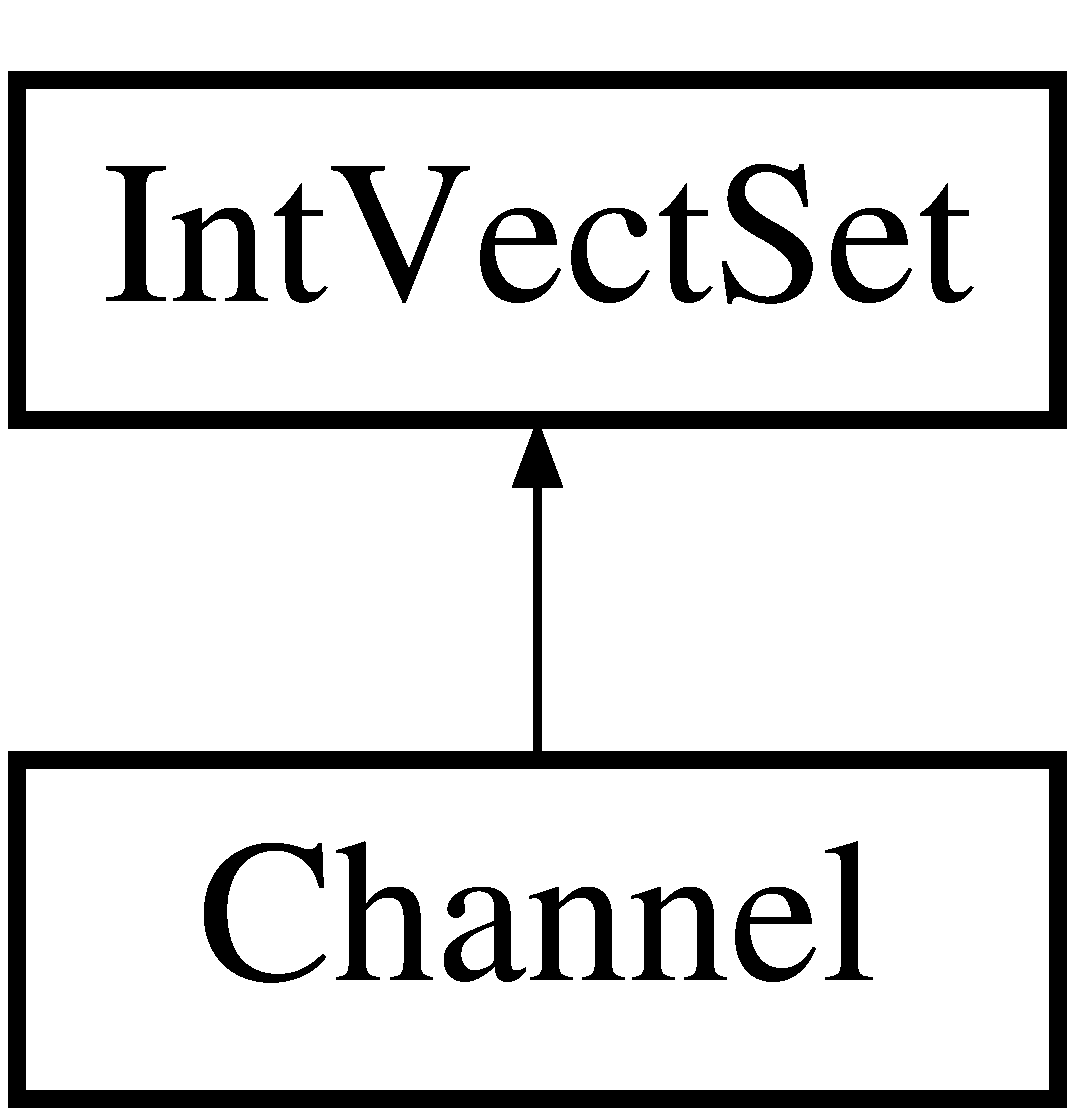
\includegraphics[height=2.000000cm]{class_channel}
\end{center}
\end{figure}
\subsection*{Public Member Functions}
\begin{DoxyCompactItemize}
\item 
\hypertarget{class_channel_a80cbe21d69e3b524a126b5a0665ecffc}{{\bfseries Channel} (const Int\-Vect \&iv)}\label{class_channel_a80cbe21d69e3b524a126b5a0665ecffc}

\item 
\hypertarget{class_channel_a7de646c5752623df873facb0172ceb25}{bool \hyperlink{class_channel_a7de646c5752623df873facb0172ceb25}{borders} (const Int\-Vect \&iv)}\label{class_channel_a7de646c5752623df873facb0172ceb25}

\begin{DoxyCompactList}\small\item\em Does this channel border the intvect? \end{DoxyCompactList}\item 
\hypertarget{class_channel_af98ac8c6c72edc3b8591bd0e043a2aa2}{Real \hyperlink{class_channel_af98ac8c6c72edc3b8591bd0e043a2aa2}{width} (Side\-::\-Lo\-Hi\-Side a\-\_\-side, int a\-\_\-offset, Real a\-\_\-dx)}\label{class_channel_af98ac8c6c72edc3b8591bd0e043a2aa2}

\begin{DoxyCompactList}\small\item\em Get the width at the vertical position specified. \end{DoxyCompactList}\item 
\hypertarget{class_channel_ab65c9b664c6772a0dd9d08cc0215030c}{Real {\bfseries height} (Real a\-\_\-dx)}\label{class_channel_ab65c9b664c6772a0dd9d08cc0215030c}

\item 
\hypertarget{class_channel_a69386c5177bdc4e2cc986e32e620e3b0}{Real {\bfseries average\-Width} (Real a\-\_\-dx)}\label{class_channel_a69386c5177bdc4e2cc986e32e620e3b0}

\item 
Real \hyperlink{class_channel_abaeb092cb3b9705a69f6c1bb26d50aa4}{location} ()
\begin{DoxyCompactList}\small\item\em Horizontal position in grid. \end{DoxyCompactList}\item 
\hypertarget{class_channel_a4c6e4cec9b33ddbdbeade8787c3e80b6}{void \hyperlink{class_channel_a4c6e4cec9b33ddbdbeade8787c3e80b6}{remove\-Bottom\-Cells} ()}\label{class_channel_a4c6e4cec9b33ddbdbeade8787c3e80b6}

\begin{DoxyCompactList}\small\item\em Remove bottom row of cells. \end{DoxyCompactList}\item 
\hypertarget{class_channel_ae46d657b8f6d3af08c2d724d6b74f360}{bool {\bfseries is\-Finished} ()}\label{class_channel_ae46d657b8f6d3af08c2d724d6b74f360}

\item 
\hypertarget{class_channel_ae872e9e8559f93f901dd0d54e3014d6f}{void {\bfseries set\-Finished} ()}\label{class_channel_ae872e9e8559f93f901dd0d54e3014d6f}

\end{DoxyCompactItemize}
\subsection*{Static Public Member Functions}
\begin{DoxyCompactItemize}
\item 
\hypertarget{class_channel_a076ddf7dc30c3fe797c3095390d1cff7}{static void {\bfseries channel\-Spacing} (Vector$<$ Real $>$ \&a\-\_\-spacing, Vector$<$ \hyperlink{class_channel}{Channel} $\ast$ $>$ \&a\-\_\-channels, Real a\-\_\-dx, Problem\-Domain a\-\_\-prob\-Domain)}\label{class_channel_a076ddf7dc30c3fe797c3095390d1cff7}

\end{DoxyCompactItemize}


\subsection{Detailed Description}
Representation of a brine channel. 

Consider a channel as just a collection of Int\-Vects (an Int\-Vect\-Set) but with a few other helpful functions e.\-g. calculating the width 

\subsection{Member Function Documentation}
\hypertarget{class_channel_abaeb092cb3b9705a69f6c1bb26d50aa4}{\index{Channel@{Channel}!location@{location}}
\index{location@{location}!Channel@{Channel}}
\subsubsection[{location}]{\setlength{\rightskip}{0pt plus 5cm}Real Channel\-::location (
\begin{DoxyParamCaption}
{}
\end{DoxyParamCaption}
)}}\label{class_channel_abaeb092cb3b9705a69f6c1bb26d50aa4}


Horizontal position in grid. 

Implicit assumption here is all channels are symmetric 

The documentation for this class was generated from the following files\-:\begin{DoxyCompactItemize}
\item 
/home/parkinsonjl/mushy-\/layer/src/Channel.\-h\item 
/home/parkinsonjl/mushy-\/layer/src/Channel.\-cpp\end{DoxyCompactItemize}

\hypertarget{class_coarse_average_edge}{\section{Coarse\-Average\-Edge Class Reference}
\label{class_coarse_average_edge}\index{Coarse\-Average\-Edge@{Coarse\-Average\-Edge}}
}


replaces edge-\/centered coarse-\/level data w/ averaged fine-\/level data  




{\ttfamily \#include $<$Coarse\-Average\-Edge.\-H$>$}

\subsection*{Public Member Functions}
\begin{DoxyCompactItemize}
\item 
\hypertarget{class_coarse_average_edge_ab19f8a588cdb3b2ecaacd58e0340aa6d}{\hyperlink{class_coarse_average_edge_ab19f8a588cdb3b2ecaacd58e0340aa6d}{Coarse\-Average\-Edge} ()}\label{class_coarse_average_edge_ab19f8a588cdb3b2ecaacd58e0340aa6d}

\begin{DoxyCompactList}\small\item\em Default constructor. \end{DoxyCompactList}\item 
\hypertarget{class_coarse_average_edge_a587bc75ddb480a189e5e619a3b23dc62}{\hyperlink{class_coarse_average_edge_a587bc75ddb480a189e5e619a3b23dc62}{Coarse\-Average\-Edge} (const Disjoint\-Box\-Layout \&a\-\_\-fine\-Grids, int a\-\_\-n\-Comp, int a\-\_\-n\-Ref)}\label{class_coarse_average_edge_a587bc75ddb480a189e5e619a3b23dc62}

\begin{DoxyCompactList}\small\item\em defining constructor \end{DoxyCompactList}\item 
\hypertarget{class_coarse_average_edge_a9f9f40f39d1de2bee0f060e8a1829df6}{\hyperlink{class_coarse_average_edge_a9f9f40f39d1de2bee0f060e8a1829df6}{$\sim$\-Coarse\-Average\-Edge} ()}\label{class_coarse_average_edge_a9f9f40f39d1de2bee0f060e8a1829df6}

\begin{DoxyCompactList}\small\item\em destructor \end{DoxyCompactList}\item 
\hypertarget{class_coarse_average_edge_afd652746f2915f00ed0b2aaad8888f4f}{void \hyperlink{class_coarse_average_edge_afd652746f2915f00ed0b2aaad8888f4f}{define} (const Disjoint\-Box\-Layout \&a\-\_\-fine\-Grids, int a\-\_\-n\-Comp, int a\-\_\-n\-Ref)}\label{class_coarse_average_edge_afd652746f2915f00ed0b2aaad8888f4f}

\begin{DoxyCompactList}\small\item\em defines the object \end{DoxyCompactList}\item 
\hypertarget{class_coarse_average_edge_acb4c74b4b3af18340fffd63b9e088efe}{bool \hyperlink{class_coarse_average_edge_acb4c74b4b3af18340fffd63b9e088efe}{is\-Defined} () const }\label{class_coarse_average_edge_acb4c74b4b3af18340fffd63b9e088efe}

\begin{DoxyCompactList}\small\item\em is object defined? \end{DoxyCompactList}\item 
\hypertarget{class_coarse_average_edge_a66df1f9dfcd7c36e5f03c777ad3889fb}{void \hyperlink{class_coarse_average_edge_a66df1f9dfcd7c36e5f03c777ad3889fb}{average\-To\-Coarse} (Level\-Data$<$ Flux\-Box $>$ \&a\-\_\-coarse\-\_\-data, const Level\-Data$<$ Flux\-Box $>$ \&a\-\_\-fine\-\_\-data)}\label{class_coarse_average_edge_a66df1f9dfcd7c36e5f03c777ad3889fb}

\begin{DoxyCompactList}\small\item\em averages fine-\/level data to coarse level \end{DoxyCompactList}\end{DoxyCompactItemize}
\subsection*{Protected Member Functions}
\begin{DoxyCompactItemize}
\item 
\hypertarget{class_coarse_average_edge_a9da8d288b5030bce697f2a862e2e0732}{void \hyperlink{class_coarse_average_edge_a9da8d288b5030bce697f2a862e2e0732}{average\-Grid\-Data} (Flux\-Box \&a\-\_\-coarsened\-Fine, const Flux\-Box \&fine) const }\label{class_coarse_average_edge_a9da8d288b5030bce697f2a862e2e0732}

\begin{DoxyCompactList}\small\item\em averages entire single grid data from fine-\/$>$crse \end{DoxyCompactList}\end{DoxyCompactItemize}
\subsection*{Protected Attributes}
\begin{DoxyCompactItemize}
\item 
\hypertarget{class_coarse_average_edge_a4a9be01bec3331bb86caceb272a8e7ea}{bool \hyperlink{class_coarse_average_edge_a4a9be01bec3331bb86caceb272a8e7ea}{m\-\_\-is\-Defined}}\label{class_coarse_average_edge_a4a9be01bec3331bb86caceb272a8e7ea}

\begin{DoxyCompactList}\small\item\em is object defined? \end{DoxyCompactList}\item 
\hypertarget{class_coarse_average_edge_a3a1d2d45d28e7b8c06287c0f5cc5cdd6}{int \hyperlink{class_coarse_average_edge_a3a1d2d45d28e7b8c06287c0f5cc5cdd6}{m\-\_\-n\-Ref}}\label{class_coarse_average_edge_a3a1d2d45d28e7b8c06287c0f5cc5cdd6}

\begin{DoxyCompactList}\small\item\em refinement ratio \end{DoxyCompactList}\item 
\hypertarget{class_coarse_average_edge_a4a8c9e61ce976a3e28ec52bb8ff78a64}{Level\-Data$<$ Flux\-Box $>$ \hyperlink{class_coarse_average_edge_a4a8c9e61ce976a3e28ec52bb8ff78a64}{m\-\_\-coarsened\-Fine\-Data}}\label{class_coarse_average_edge_a4a8c9e61ce976a3e28ec52bb8ff78a64}

\begin{DoxyCompactList}\small\item\em work array for coarsening of fine data, same \char`\"{}shape\char`\"{} as fine data \end{DoxyCompactList}\end{DoxyCompactItemize}


\subsection{Detailed Description}
replaces edge-\/centered coarse-\/level data w/ averaged fine-\/level data 

This class replaces edge-\/centered data on a coarse level of refinement with the average of the finer-\/level data which overlays the edge. This class is similar to Coarse\-Average 

The documentation for this class was generated from the following files\-:\begin{DoxyCompactItemize}
\item 
/home/parkinsonjl/mushy-\/layer/util/Coarse\-Average\-Edge.\-H\item 
/home/parkinsonjl/mushy-\/layer/util/Coarse\-Average\-Edge.\-cpp\end{DoxyCompactItemize}

\hypertarget{class_coefficient_interpolator_linear}{\section{Coefficient\-Interpolator\-Linear Class Reference}
\label{class_coefficient_interpolator_linear}\index{Coefficient\-Interpolator\-Linear@{Coefficient\-Interpolator\-Linear}}
}


Linear coefficient interpolator.  




{\ttfamily \#include $<$Coefficient\-Interpolator\-Linear.\-H$>$}

Inheritance diagram for Coefficient\-Interpolator\-Linear\-:\begin{figure}[H]
\begin{center}
\leavevmode
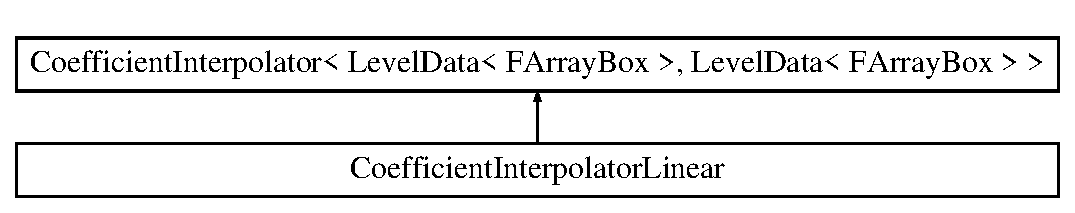
\includegraphics[height=2.000000cm]{class_coefficient_interpolator_linear}
\end{center}
\end{figure}
\subsection*{Public Member Functions}
\begin{DoxyCompactItemize}
\item 
\hypertarget{class_coefficient_interpolator_linear_a99f4253fee5e273890ca1dbf9f9ff60e}{\hyperlink{class_coefficient_interpolator_linear_a99f4253fee5e273890ca1dbf9f9ff60e}{Coefficient\-Interpolator\-Linear} (int a\-\_\-num\-Comps=1)}\label{class_coefficient_interpolator_linear_a99f4253fee5e273890ca1dbf9f9ff60e}

\begin{DoxyCompactList}\small\item\em default constructor \end{DoxyCompactList}\item 
\hypertarget{class_coefficient_interpolator_linear_ae9e668747f2c5a702d022c26d27ceb3a}{virtual void \hyperlink{class_coefficient_interpolator_linear_ae9e668747f2c5a702d022c26d27ceb3a}{interpolate} (Level\-Data$<$ F\-Array\-Box $>$ \&a\-\_\-result, Real a\-\_\-time)}\label{class_coefficient_interpolator_linear_ae9e668747f2c5a702d022c26d27ceb3a}

\begin{DoxyCompactList}\small\item\em Interpolate in time. \end{DoxyCompactList}\item 
virtual void \hyperlink{class_coefficient_interpolator_linear_a7558771f5d460bb587cc8f90c0156b1f}{interpolate} (Level\-Data$<$ F\-Array\-Box $>$ \&a\-\_\-result, const Level\-Data$<$ F\-Array\-Box $>$ \&a\-\_\-solution, Real a\-\_\-time)
\item 
virtual bool \hyperlink{class_coefficient_interpolator_linear_a498be7688cfdc0831606822cfde2de24}{depends\-Upon\-Solution} () const 
\item 
virtual void \hyperlink{class_coefficient_interpolator_linear_a86904e8968464cbeaf2c5dbae76f7545}{interpolate\-Prime} (Level\-Data$<$ F\-Array\-Box $>$ \&a\-\_\-prime, const Level\-Data$<$ F\-Array\-Box $>$ \&a\-\_\-solution, Real a\-\_\-time)
\item 
virtual void \hyperlink{class_coefficient_interpolator_linear_ab1c2295a8ed1749ad55dd366bde4139a}{solve} (Level\-Data$<$ F\-Array\-Box $>$ \&a\-\_\-phi, const Level\-Data$<$ F\-Array\-Box $>$ \&a\-\_\-f, Real a\-\_\-time, const Level\-Data$<$ F\-Array\-Box $>$ \&a\-\_\-phi0, Real a\-\_\-tolerance)
\item 
\hypertarget{class_coefficient_interpolator_linear_af6983e0b6efb89666c6e163db00aa79c}{void \hyperlink{class_coefficient_interpolator_linear_af6983e0b6efb89666c6e163db00aa79c}{define} (Ref\-Counted\-Ptr$<$ Level\-Data$<$ F\-Array\-Box $>$ $>$ a\-\_\-coef\-Old, Ref\-Counted\-Ptr$<$ Level\-Data$<$ F\-Array\-Box $>$ $>$ a\-\_\-coef\-New, Real a\-\_\-time\-Old, Real a\-\_\-time\-New)}\label{class_coefficient_interpolator_linear_af6983e0b6efb89666c6e163db00aa79c}

\begin{DoxyCompactList}\small\item\em Define coefficients. \end{DoxyCompactList}\end{DoxyCompactItemize}
\subsection*{Public Attributes}
\begin{DoxyCompactItemize}
\item 
\hypertarget{class_coefficient_interpolator_linear_a4f859c7c7aa5fefe581e70b641c2c7cd}{Ref\-Counted\-Ptr$<$ Level\-Data\\*
$<$ F\-Array\-Box $>$ $>$ \hyperlink{class_coefficient_interpolator_linear_a4f859c7c7aa5fefe581e70b641c2c7cd}{m\-\_\-coef\-Old}}\label{class_coefficient_interpolator_linear_a4f859c7c7aa5fefe581e70b641c2c7cd}

\begin{DoxyCompactList}\small\item\em Coefficient at old time. \end{DoxyCompactList}\item 
\hypertarget{class_coefficient_interpolator_linear_ab139ee5bd26c87a907242072d79080e2}{Ref\-Counted\-Ptr$<$ Level\-Data\\*
$<$ F\-Array\-Box $>$ $>$ \hyperlink{class_coefficient_interpolator_linear_ab139ee5bd26c87a907242072d79080e2}{m\-\_\-coef\-New}}\label{class_coefficient_interpolator_linear_ab139ee5bd26c87a907242072d79080e2}

\begin{DoxyCompactList}\small\item\em Coefficient at new time. \end{DoxyCompactList}\item 
\hypertarget{class_coefficient_interpolator_linear_a2ab6b22fe2ae4b4a67c2b2e8939a7725}{Real \hyperlink{class_coefficient_interpolator_linear_a2ab6b22fe2ae4b4a67c2b2e8939a7725}{m\-\_\-time\-Old}}\label{class_coefficient_interpolator_linear_a2ab6b22fe2ae4b4a67c2b2e8939a7725}

\begin{DoxyCompactList}\small\item\em Old time. \end{DoxyCompactList}\item 
\hypertarget{class_coefficient_interpolator_linear_a6202c9344b2886cf3a951e8aed4c9dbd}{Real \hyperlink{class_coefficient_interpolator_linear_a6202c9344b2886cf3a951e8aed4c9dbd}{m\-\_\-time\-New}}\label{class_coefficient_interpolator_linear_a6202c9344b2886cf3a951e8aed4c9dbd}

\begin{DoxyCompactList}\small\item\em New time. \end{DoxyCompactList}\end{DoxyCompactItemize}


\subsection{Detailed Description}
Linear coefficient interpolator. 

Class to get time depdendent coefficients by interpolating linearly in time. 

\subsection{Member Function Documentation}
\hypertarget{class_coefficient_interpolator_linear_a498be7688cfdc0831606822cfde2de24}{\index{Coefficient\-Interpolator\-Linear@{Coefficient\-Interpolator\-Linear}!depends\-Upon\-Solution@{depends\-Upon\-Solution}}
\index{depends\-Upon\-Solution@{depends\-Upon\-Solution}!CoefficientInterpolatorLinear@{Coefficient\-Interpolator\-Linear}}
\subsubsection[{depends\-Upon\-Solution}]{\setlength{\rightskip}{0pt plus 5cm}bool Coefficient\-Interpolator\-Linear\-::depends\-Upon\-Solution (
\begin{DoxyParamCaption}
{}
\end{DoxyParamCaption}
) const\hspace{0.3cm}{\ttfamily [virtual]}}}\label{class_coefficient_interpolator_linear_a498be7688cfdc0831606822cfde2de24}
Returns true if the coefficient depends on the solution to the partial differential equation (rendering it nonlinear), false otherwise. By default, the coefficient is assumed not to depend upon the solution. \hypertarget{class_coefficient_interpolator_linear_a7558771f5d460bb587cc8f90c0156b1f}{\index{Coefficient\-Interpolator\-Linear@{Coefficient\-Interpolator\-Linear}!interpolate@{interpolate}}
\index{interpolate@{interpolate}!CoefficientInterpolatorLinear@{Coefficient\-Interpolator\-Linear}}
\subsubsection[{interpolate}]{\setlength{\rightskip}{0pt plus 5cm}void Coefficient\-Interpolator\-Linear\-::interpolate (
\begin{DoxyParamCaption}
\item[{Level\-Data$<$ F\-Array\-Box $>$ \&}]{a\-\_\-result, }
\item[{const Level\-Data$<$ F\-Array\-Box $>$ \&}]{a\-\_\-solution, }
\item[{Real}]{a\-\_\-time}
\end{DoxyParamCaption}
)\hspace{0.3cm}{\ttfamily [virtual]}}}\label{class_coefficient_interpolator_linear_a7558771f5d460bb587cc8f90c0156b1f}
Interpolate the coefficient at the given time, placing the result in the given Level\-Data object. This method assumes that the coefficient depends upon the solution to the partial differential equation in question, so the solution is passed into it as an argument. 
\begin{DoxyParams}{Parameters}
{\em a\-\_\-result} & The Level\-Data object that will store the result. \\
\hline
{\em a\-\_\-solution} & The solution to the partial differential equation. \\
\hline
{\em a\-\_\-time} & The time at which the coefficient is to be evaluated. \\
\hline
\end{DoxyParams}
\hypertarget{class_coefficient_interpolator_linear_a86904e8968464cbeaf2c5dbae76f7545}{\index{Coefficient\-Interpolator\-Linear@{Coefficient\-Interpolator\-Linear}!interpolate\-Prime@{interpolate\-Prime}}
\index{interpolate\-Prime@{interpolate\-Prime}!CoefficientInterpolatorLinear@{Coefficient\-Interpolator\-Linear}}
\subsubsection[{interpolate\-Prime}]{\setlength{\rightskip}{0pt plus 5cm}void Coefficient\-Interpolator\-Linear\-::interpolate\-Prime (
\begin{DoxyParamCaption}
\item[{Level\-Data$<$ F\-Array\-Box $>$ \&}]{a\-\_\-prime, }
\item[{const Level\-Data$<$ F\-Array\-Box $>$ \&}]{a\-\_\-solution, }
\item[{Real}]{a\-\_\-time}
\end{DoxyParamCaption}
)\hspace{0.3cm}{\ttfamily [virtual]}}}\label{class_coefficient_interpolator_linear_a86904e8968464cbeaf2c5dbae76f7545}
Computes the derivative of the coefficient with respect to the solution at the desired time. By default, this sets {\itshape a\-\_\-deriv} to 0. 
\begin{DoxyParams}{Parameters}
{\em a\-\_\-prime} & The coefficient derivative data will be stored here. \\
\hline
{\em a\-\_\-solution} & The solution to the partial differential equation. \\
\hline
{\em a\-\_\-time} & The time at which to compute the coefficient data. \\
\hline
\end{DoxyParams}
\hypertarget{class_coefficient_interpolator_linear_ab1c2295a8ed1749ad55dd366bde4139a}{\index{Coefficient\-Interpolator\-Linear@{Coefficient\-Interpolator\-Linear}!solve@{solve}}
\index{solve@{solve}!CoefficientInterpolatorLinear@{Coefficient\-Interpolator\-Linear}}
\subsubsection[{solve}]{\setlength{\rightskip}{0pt plus 5cm}void Coefficient\-Interpolator\-Linear\-::solve (
\begin{DoxyParamCaption}
\item[{Level\-Data$<$ F\-Array\-Box $>$ \&}]{a\-\_\-phi, }
\item[{const Level\-Data$<$ F\-Array\-Box $>$ \&}]{a\-\_\-f, }
\item[{Real}]{a\-\_\-time, }
\item[{const Level\-Data$<$ F\-Array\-Box $>$ \&}]{a\-\_\-phi0, }
\item[{Real}]{a\-\_\-tolerance}
\end{DoxyParamCaption}
)\hspace{0.3cm}{\ttfamily [virtual]}}}\label{class_coefficient_interpolator_linear_ab1c2295a8ed1749ad55dd366bde4139a}
This virtual void method performs the iterative nonlinear solve $A(\phi) \phi - f(\vec{x}) = 0$ for $\phi$. 
\begin{DoxyParams}{Parameters}
{\em a\-\_\-phi} & The solution to the equation, $\phi$, will be stored here. \\
\hline
{\em a\-\_\-f} & The term $f(\vec{x})$ in the equation. \\
\hline
{\em a\-\_\-time} & The time at which the equation is solved. \\
\hline
{\em a\-\_\-phi0} & The initial estimate for $\phi$. \\
\hline
{\em a\-\_\-tolerance} & The threshold for the error in the equation that dictates when iteration should cease. \\
\hline
\end{DoxyParams}


The documentation for this class was generated from the following files\-:\begin{DoxyCompactItemize}
\item 
/home/parkinsonjl/mushy-\/layer/src/Coefficient\-Interpolator\-Linear.\-H\item 
/home/parkinsonjl/mushy-\/layer/src/Coefficient\-Interpolator\-Linear.\-cpp\end{DoxyCompactItemize}

\hypertarget{class_coefficient_interpolator_linear_face}{\section{Coefficient\-Interpolator\-Linear\-Face Class Reference}
\label{class_coefficient_interpolator_linear_face}\index{Coefficient\-Interpolator\-Linear\-Face@{Coefficient\-Interpolator\-Linear\-Face}}
}


Linear coefficient interpolator (face centred)  




{\ttfamily \#include $<$Coefficient\-Interpolator\-Linear\-Face.\-H$>$}

Inheritance diagram for Coefficient\-Interpolator\-Linear\-Face\-:\begin{figure}[H]
\begin{center}
\leavevmode
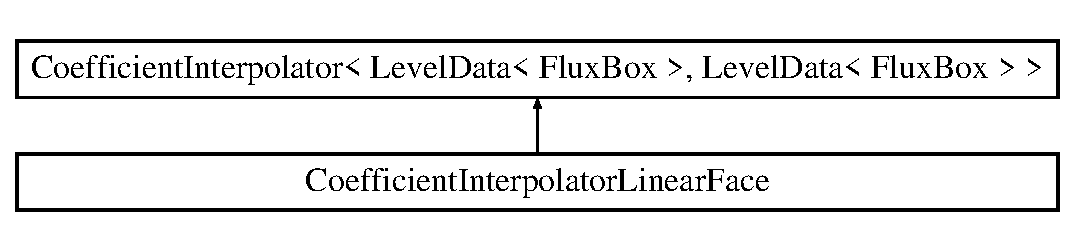
\includegraphics[height=2.000000cm]{class_coefficient_interpolator_linear_face}
\end{center}
\end{figure}
\subsection*{Public Member Functions}
\begin{DoxyCompactItemize}
\item 
\hypertarget{class_coefficient_interpolator_linear_face_a64b4959fa8d8df6705df5a8baf31f3f5}{\hyperlink{class_coefficient_interpolator_linear_face_a64b4959fa8d8df6705df5a8baf31f3f5}{Coefficient\-Interpolator\-Linear\-Face} (int a\-\_\-num\-Comps=1)}\label{class_coefficient_interpolator_linear_face_a64b4959fa8d8df6705df5a8baf31f3f5}

\begin{DoxyCompactList}\small\item\em default constructor \end{DoxyCompactList}\item 
\hypertarget{class_coefficient_interpolator_linear_face_a08d5f51d4204deb361b6c8cb054cff69}{virtual void \hyperlink{class_coefficient_interpolator_linear_face_a08d5f51d4204deb361b6c8cb054cff69}{interpolate} (Level\-Data$<$ Flux\-Box $>$ \&a\-\_\-result, Real a\-\_\-time)}\label{class_coefficient_interpolator_linear_face_a08d5f51d4204deb361b6c8cb054cff69}

\begin{DoxyCompactList}\small\item\em Interpolate coefficient. \end{DoxyCompactList}\item 
virtual void \hyperlink{class_coefficient_interpolator_linear_face_a825a5def3f5da9e2a8890bd46d2af5b0}{interpolate} (Level\-Data$<$ Flux\-Box $>$ \&a\-\_\-result, const Level\-Data$<$ Flux\-Box $>$ \&a\-\_\-solution, Real a\-\_\-time)
\item 
virtual bool \hyperlink{class_coefficient_interpolator_linear_face_a233d0b610df69e882c5820610dc65f99}{depends\-Upon\-Solution} () const 
\item 
virtual void \hyperlink{class_coefficient_interpolator_linear_face_a6a9d41e8aac928cad20649644ce70aeb}{interpolate\-Prime} (Level\-Data$<$ Flux\-Box $>$ \&a\-\_\-prime, const Level\-Data$<$ Flux\-Box $>$ \&a\-\_\-solution, Real a\-\_\-time)
\item 
virtual void \hyperlink{class_coefficient_interpolator_linear_face_aa1d2b29813de7845fda24e5c523ca5b7}{solve} (Level\-Data$<$ Flux\-Box $>$ \&a\-\_\-phi, const Level\-Data$<$ Flux\-Box $>$ \&a\-\_\-f, Real a\-\_\-time, const Level\-Data$<$ Flux\-Box $>$ \&a\-\_\-phi0, Real a\-\_\-tolerance)
\item 
\hypertarget{class_coefficient_interpolator_linear_face_af27d8bed697ac3ddda5accdd37df3dee}{void \hyperlink{class_coefficient_interpolator_linear_face_af27d8bed697ac3ddda5accdd37df3dee}{define} (Ref\-Counted\-Ptr$<$ Level\-Data$<$ Flux\-Box $>$ $>$ a\-\_\-coef\-Old, Ref\-Counted\-Ptr$<$ Level\-Data$<$ Flux\-Box $>$ $>$ a\-\_\-coef\-New, Real a\-\_\-time\-Old, Real a\-\_\-time\-New)}\label{class_coefficient_interpolator_linear_face_af27d8bed697ac3ddda5accdd37df3dee}

\begin{DoxyCompactList}\small\item\em Define. \end{DoxyCompactList}\end{DoxyCompactItemize}
\subsection*{Public Attributes}
\begin{DoxyCompactItemize}
\item 
\hypertarget{class_coefficient_interpolator_linear_face_aae51740c3e19c958371b6b1136f8d9c1}{Ref\-Counted\-Ptr$<$ Level\-Data\\*
$<$ Flux\-Box $>$ $>$ \hyperlink{class_coefficient_interpolator_linear_face_aae51740c3e19c958371b6b1136f8d9c1}{m\-\_\-coef\-Old}}\label{class_coefficient_interpolator_linear_face_aae51740c3e19c958371b6b1136f8d9c1}

\begin{DoxyCompactList}\small\item\em Coefficient at old time. \end{DoxyCompactList}\item 
\hypertarget{class_coefficient_interpolator_linear_face_a8211cb341ee6772d07fc4951aab16a00}{Ref\-Counted\-Ptr$<$ Level\-Data\\*
$<$ Flux\-Box $>$ $>$ \hyperlink{class_coefficient_interpolator_linear_face_a8211cb341ee6772d07fc4951aab16a00}{m\-\_\-coef\-New}}\label{class_coefficient_interpolator_linear_face_a8211cb341ee6772d07fc4951aab16a00}

\begin{DoxyCompactList}\small\item\em Coefficient at new time. \end{DoxyCompactList}\item 
\hypertarget{class_coefficient_interpolator_linear_face_aa4b51decdda11a34c0d910cd1be109bd}{Real \hyperlink{class_coefficient_interpolator_linear_face_aa4b51decdda11a34c0d910cd1be109bd}{m\-\_\-time\-Old}}\label{class_coefficient_interpolator_linear_face_aa4b51decdda11a34c0d910cd1be109bd}

\begin{DoxyCompactList}\small\item\em Old time. \end{DoxyCompactList}\item 
\hypertarget{class_coefficient_interpolator_linear_face_af4baef6ce288a442d798fe1650b9a932}{Real \hyperlink{class_coefficient_interpolator_linear_face_af4baef6ce288a442d798fe1650b9a932}{m\-\_\-time\-New}}\label{class_coefficient_interpolator_linear_face_af4baef6ce288a442d798fe1650b9a932}

\begin{DoxyCompactList}\small\item\em New time. \end{DoxyCompactList}\end{DoxyCompactItemize}


\subsection{Detailed Description}
Linear coefficient interpolator (face centred) 

Class to get time depdendent (face centred) coefficients by interpolating linearly in time. 

\subsection{Member Function Documentation}
\hypertarget{class_coefficient_interpolator_linear_face_a233d0b610df69e882c5820610dc65f99}{\index{Coefficient\-Interpolator\-Linear\-Face@{Coefficient\-Interpolator\-Linear\-Face}!depends\-Upon\-Solution@{depends\-Upon\-Solution}}
\index{depends\-Upon\-Solution@{depends\-Upon\-Solution}!CoefficientInterpolatorLinearFace@{Coefficient\-Interpolator\-Linear\-Face}}
\subsubsection[{depends\-Upon\-Solution}]{\setlength{\rightskip}{0pt plus 5cm}bool Coefficient\-Interpolator\-Linear\-Face\-::depends\-Upon\-Solution (
\begin{DoxyParamCaption}
{}
\end{DoxyParamCaption}
) const\hspace{0.3cm}{\ttfamily [virtual]}}}\label{class_coefficient_interpolator_linear_face_a233d0b610df69e882c5820610dc65f99}
Returns true if the coefficient depends on the solution to the partial differential equation (rendering it nonlinear), false otherwise. By default, the coefficient is assumed not to depend upon the solution. \hypertarget{class_coefficient_interpolator_linear_face_a825a5def3f5da9e2a8890bd46d2af5b0}{\index{Coefficient\-Interpolator\-Linear\-Face@{Coefficient\-Interpolator\-Linear\-Face}!interpolate@{interpolate}}
\index{interpolate@{interpolate}!CoefficientInterpolatorLinearFace@{Coefficient\-Interpolator\-Linear\-Face}}
\subsubsection[{interpolate}]{\setlength{\rightskip}{0pt plus 5cm}void Coefficient\-Interpolator\-Linear\-Face\-::interpolate (
\begin{DoxyParamCaption}
\item[{Level\-Data$<$ Flux\-Box $>$ \&}]{a\-\_\-result, }
\item[{const Level\-Data$<$ Flux\-Box $>$ \&}]{a\-\_\-solution, }
\item[{Real}]{a\-\_\-time}
\end{DoxyParamCaption}
)\hspace{0.3cm}{\ttfamily [virtual]}}}\label{class_coefficient_interpolator_linear_face_a825a5def3f5da9e2a8890bd46d2af5b0}
Interpolate the coefficient at the given time, placing the result in the given Level\-Data object. This method assumes that the coefficient depends upon the solution to the partial differential equation in question, so the solution is passed into it as an argument. 
\begin{DoxyParams}{Parameters}
{\em a\-\_\-result} & The Level\-Data object that will store the result. \\
\hline
{\em a\-\_\-solution} & The solution to the partial differential equation. \\
\hline
{\em a\-\_\-time} & The time at which the coefficient is to be evaluated. \\
\hline
\end{DoxyParams}
\hypertarget{class_coefficient_interpolator_linear_face_a6a9d41e8aac928cad20649644ce70aeb}{\index{Coefficient\-Interpolator\-Linear\-Face@{Coefficient\-Interpolator\-Linear\-Face}!interpolate\-Prime@{interpolate\-Prime}}
\index{interpolate\-Prime@{interpolate\-Prime}!CoefficientInterpolatorLinearFace@{Coefficient\-Interpolator\-Linear\-Face}}
\subsubsection[{interpolate\-Prime}]{\setlength{\rightskip}{0pt plus 5cm}void Coefficient\-Interpolator\-Linear\-Face\-::interpolate\-Prime (
\begin{DoxyParamCaption}
\item[{Level\-Data$<$ Flux\-Box $>$ \&}]{a\-\_\-prime, }
\item[{const Level\-Data$<$ Flux\-Box $>$ \&}]{a\-\_\-solution, }
\item[{Real}]{a\-\_\-time}
\end{DoxyParamCaption}
)\hspace{0.3cm}{\ttfamily [virtual]}}}\label{class_coefficient_interpolator_linear_face_a6a9d41e8aac928cad20649644ce70aeb}
Computes the derivative of the coefficient with respect to the solution at the desired time. By default, this sets {\itshape a\-\_\-deriv} to 0. 
\begin{DoxyParams}{Parameters}
{\em a\-\_\-prime} & The coefficient derivative data will be stored here. \\
\hline
{\em a\-\_\-solution} & The solution to the partial differential equation. \\
\hline
{\em a\-\_\-time} & The time at which to compute the coefficient data. \\
\hline
\end{DoxyParams}
\hypertarget{class_coefficient_interpolator_linear_face_aa1d2b29813de7845fda24e5c523ca5b7}{\index{Coefficient\-Interpolator\-Linear\-Face@{Coefficient\-Interpolator\-Linear\-Face}!solve@{solve}}
\index{solve@{solve}!CoefficientInterpolatorLinearFace@{Coefficient\-Interpolator\-Linear\-Face}}
\subsubsection[{solve}]{\setlength{\rightskip}{0pt plus 5cm}void Coefficient\-Interpolator\-Linear\-Face\-::solve (
\begin{DoxyParamCaption}
\item[{Level\-Data$<$ Flux\-Box $>$ \&}]{a\-\_\-phi, }
\item[{const Level\-Data$<$ Flux\-Box $>$ \&}]{a\-\_\-f, }
\item[{Real}]{a\-\_\-time, }
\item[{const Level\-Data$<$ Flux\-Box $>$ \&}]{a\-\_\-phi0, }
\item[{Real}]{a\-\_\-tolerance}
\end{DoxyParamCaption}
)\hspace{0.3cm}{\ttfamily [virtual]}}}\label{class_coefficient_interpolator_linear_face_aa1d2b29813de7845fda24e5c523ca5b7}
This virtual void method performs the iterative nonlinear solve $A(\phi) \phi - f(\vec{x}) = 0$ for $\phi$. 
\begin{DoxyParams}{Parameters}
{\em a\-\_\-phi} & The solution to the equation, $\phi$, will be stored here. \\
\hline
{\em a\-\_\-f} & The term $f(\vec{x})$ in the equation. \\
\hline
{\em a\-\_\-time} & The time at which the equation is solved. \\
\hline
{\em a\-\_\-phi0} & The initial estimate for $\phi$. \\
\hline
{\em a\-\_\-tolerance} & The threshold for the error in the equation that dictates when iteration should cease. \\
\hline
\end{DoxyParams}


The documentation for this class was generated from the following files\-:\begin{DoxyCompactItemize}
\item 
/home/parkinsonjl/mushy-\/layer/src/Coefficient\-Interpolator\-Linear\-Face.\-H\item 
/home/parkinsonjl/mushy-\/layer/src/Coefficient\-Interpolator\-Linear\-Face.\-cpp\end{DoxyCompactItemize}

\hypertarget{class_const_value_function}{\section{Const\-Value\-Function Class Reference}
\label{class_const_value_function}\index{Const\-Value\-Function@{Const\-Value\-Function}}
}


Constant value B\-C.  


Inheritance diagram for Const\-Value\-Function\-:\begin{figure}[H]
\begin{center}
\leavevmode
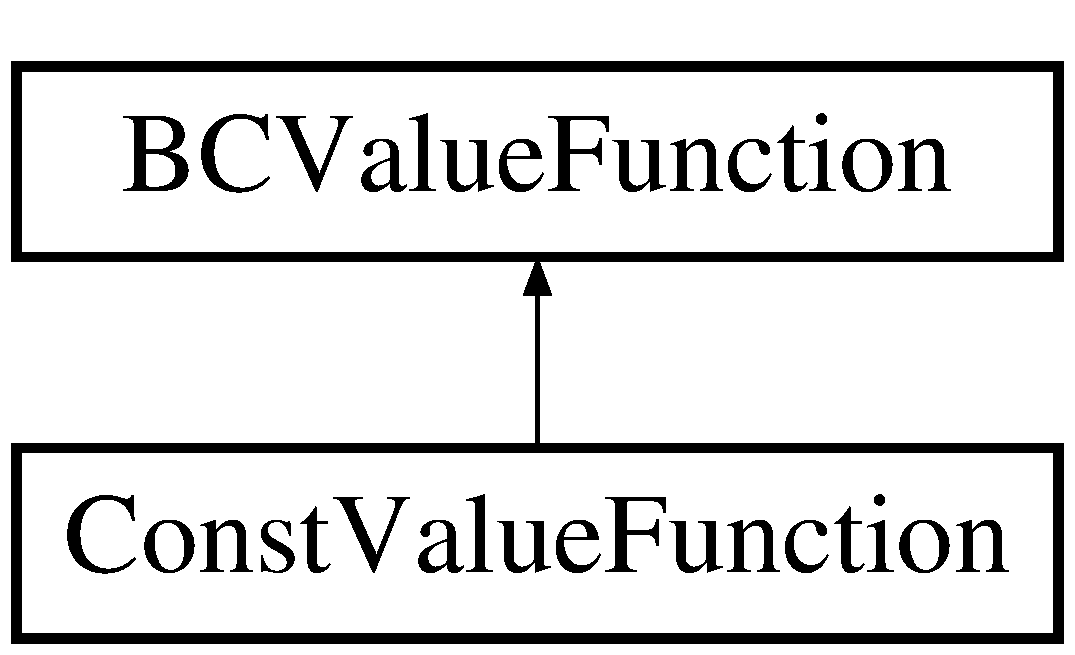
\includegraphics[height=2.000000cm]{class_const_value_function}
\end{center}
\end{figure}
\subsection*{Public Member Functions}
\begin{DoxyCompactItemize}
\item 
\hypertarget{class_const_value_function_a3022feb84ef9e65bba61c2fe27a3bcd3}{\hyperlink{class_const_value_function_a3022feb84ef9e65bba61c2fe27a3bcd3}{Const\-Value\-Function} ()}\label{class_const_value_function_a3022feb84ef9e65bba61c2fe27a3bcd3}

\begin{DoxyCompactList}\small\item\em Default constructor. \end{DoxyCompactList}\item 
\hypertarget{class_const_value_function_a2c0a36991ee9548815186ac1db46d133}{\hyperlink{class_const_value_function_a2c0a36991ee9548815186ac1db46d133}{Const\-Value\-Function} (Real a\-\_\-value, int a\-\_\-n\-Comp)}\label{class_const_value_function_a2c0a36991ee9548815186ac1db46d133}

\begin{DoxyCompactList}\small\item\em Constructor. \end{DoxyCompactList}\item 
\hypertarget{class_const_value_function_a417fb6f37a91828d252e433b3992e585}{virtual void \hyperlink{class_const_value_function_a417fb6f37a91828d252e433b3992e585}{operator()} (Real $\ast$a\-\_\-pos, int $\ast$a\-\_\-dir, Side\-::\-Lo\-Hi\-Side $\ast$a\-\_\-side, Real $\ast$a\-\_\-value)}\label{class_const_value_function_a417fb6f37a91828d252e433b3992e585}

\begin{DoxyCompactList}\small\item\em Apply B\-C. \end{DoxyCompactList}\end{DoxyCompactItemize}
\subsection*{Public Attributes}
\begin{DoxyCompactItemize}
\item 
\hypertarget{class_const_value_function_ab7eca155d9349f33bc744398a5b34def}{Real \hyperlink{class_const_value_function_ab7eca155d9349f33bc744398a5b34def}{m\-\_\-value}}\label{class_const_value_function_ab7eca155d9349f33bc744398a5b34def}

\begin{DoxyCompactList}\small\item\em The constant value to apply. \end{DoxyCompactList}\item 
\hypertarget{class_const_value_function_a9a8923f47bc33ea19749a2b60b9416e2}{int \hyperlink{class_const_value_function_a9a8923f47bc33ea19749a2b60b9416e2}{m\-\_\-n\-Comp}}\label{class_const_value_function_a9a8923f47bc33ea19749a2b60b9416e2}

\begin{DoxyCompactList}\small\item\em The component to apply this B\-C to. \end{DoxyCompactList}\end{DoxyCompactItemize}


\subsection{Detailed Description}
Constant value B\-C. 

Returns a single scalar value, independent of side or position along side, which can be different for different components. 

The documentation for this class was generated from the following file\-:\begin{DoxyCompactItemize}
\item 
/home/parkinsonjl/mushy-\/layer/\-B\-Cutil/Phys\-B\-C\-Util.\-cpp\end{DoxyCompactItemize}

\hypertarget{class_darcy_brinkman_op}{\section{Darcy\-Brinkman\-Op Class Reference}
\label{class_darcy_brinkman_op}\index{Darcy\-Brinkman\-Op@{Darcy\-Brinkman\-Op}}
}


Operator for solving the Darcy-\/\-Brinkman equation.  




{\ttfamily \#include $<$Darcy\-Brinkman\-Op.\-H$>$}

Inheritance diagram for Darcy\-Brinkman\-Op\-:\begin{figure}[H]
\begin{center}
\leavevmode
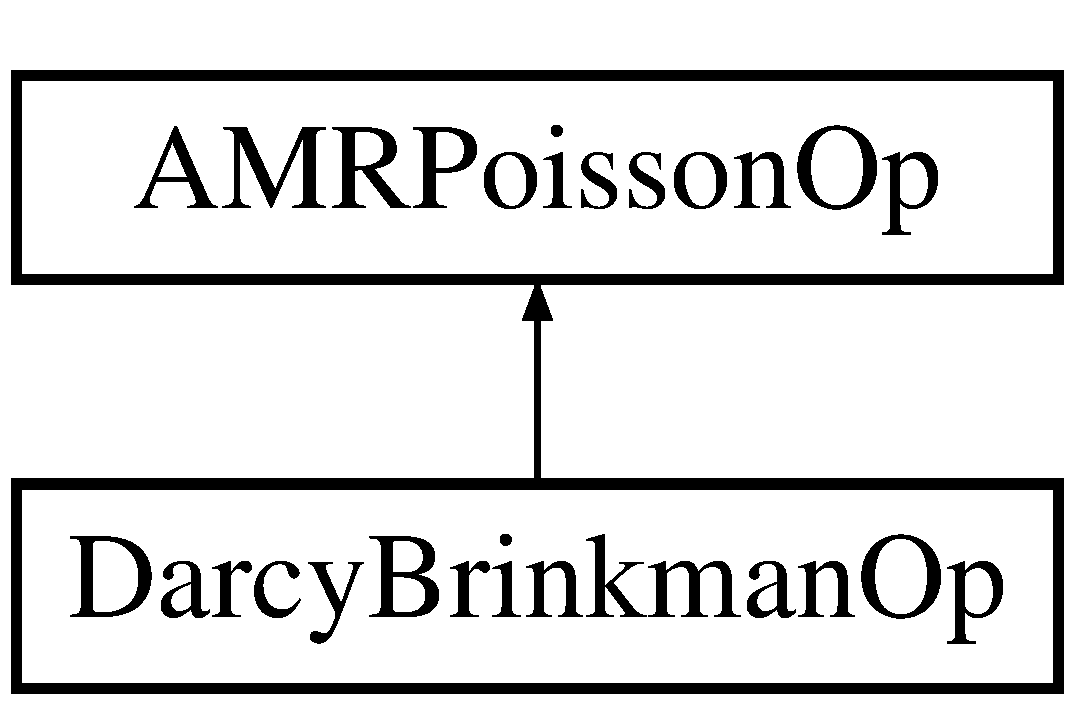
\includegraphics[height=2.000000cm]{class_darcy_brinkman_op}
\end{center}
\end{figure}
\subsection*{Public Member Functions}
\begin{DoxyCompactItemize}
\item 
void \hyperlink{class_darcy_brinkman_op_ac6da9fd6f61b40c42b3a94b645c21e35}{finer\-Operator\-Changed} (const M\-G\-Level\-Op$<$ Level\-Data$<$ F\-Array\-Box $>$ $>$ \&a\-\_\-operator, int a\-\_\-coarsening\-Factor)
\item 
\hypertarget{class_darcy_brinkman_op_a27d3f026aea19d8b7f14f6801d4fb479}{Level\-Data$<$ F\-Array\-Box $>$ \& \hyperlink{class_darcy_brinkman_op_a27d3f026aea19d8b7f14f6801d4fb479}{identity\-Coef} ()}\label{class_darcy_brinkman_op_a27d3f026aea19d8b7f14f6801d4fb479}

\begin{DoxyCompactList}\small\item\em Returns identity coefficient data. \end{DoxyCompactList}\item 
\hypertarget{class_darcy_brinkman_op_a4c661019f1436c2d7f68e6d7ec8a216c}{virtual void \hyperlink{class_darcy_brinkman_op_a4c661019f1436c2d7f68e6d7ec8a216c}{diagonal\-Scale} (Level\-Data$<$ F\-Array\-Box $>$ \&a\-\_\-rhs, bool a\-\_\-kappa\-Weighted)}\label{class_darcy_brinkman_op_a4c661019f1436c2d7f68e6d7ec8a216c}

\begin{DoxyCompactList}\small\item\em For tga stuff. \end{DoxyCompactList}\item 
\hypertarget{class_darcy_brinkman_op_a6b3aa7b8af250978e180b477a9037061}{virtual void \hyperlink{class_darcy_brinkman_op_a6b3aa7b8af250978e180b477a9037061}{divide\-By\-Identity\-Coef} (Level\-Data$<$ F\-Array\-Box $>$ \&a\-\_\-rhs)}\label{class_darcy_brinkman_op_a6b3aa7b8af250978e180b477a9037061}

\begin{DoxyCompactList}\small\item\em For tga stuff. \end{DoxyCompactList}\item 
void \hyperlink{class_darcy_brinkman_op_a291dd090a4475bcb95fe2901722660c9}{set\-B\-Coef\-Interpolator} (Ref\-Counted\-Ptr$<$ Coefficient\-Interpolator$<$ Level\-Data$<$ Flux\-Box $>$, Level\-Data$<$ F\-Array\-Box $>$ $>$ $>$ \&a\-\_\-b\-Coef\-Interpolator)
\item 
\hypertarget{class_darcy_brinkman_op_a9b2d72f39820a3dfcd502ea60232ddeb}{Level\-Data$<$ Flux\-Box $>$ \& \hyperlink{class_darcy_brinkman_op_a9b2d72f39820a3dfcd502ea60232ddeb}{B\-Coef} ()}\label{class_darcy_brinkman_op_a9b2d72f39820a3dfcd502ea60232ddeb}

\begin{DoxyCompactList}\small\item\em Returns the B coefficient. \end{DoxyCompactList}\item 
\hypertarget{class_darcy_brinkman_op_a16cce095d955f2514589e45bd6b348df}{Ref\-Counted\-Ptr\\*
$<$ Coefficient\-Interpolator\\*
$<$ Level\-Data$<$ Flux\-Box $>$\\*
, Level\-Data$<$ F\-Array\-Box $>$ $>$ $>$ \hyperlink{class_darcy_brinkman_op_a16cce095d955f2514589e45bd6b348df}{B\-Coef\-Interpolator} ()}\label{class_darcy_brinkman_op_a16cce095d955f2514589e45bd6b348df}

\begin{DoxyCompactList}\small\item\em Allows access to the B coefficient interpolator. \end{DoxyCompactList}\item 
void \hyperlink{class_darcy_brinkman_op_a50dc1353f78c310c788763b122ca939d}{set\-Time} (Real a\-\_\-time)
\item 
virtual void \hyperlink{class_darcy_brinkman_op_adfd7590e98c5edd78140265bb05eef17}{get\-Flux} (Flux\-Box \&a\-\_\-flux, const Level\-Data$<$ F\-Array\-Box $>$ \&a\-\_\-data, const Box \&a\-\_\-grid, const Data\-Index \&a\-\_\-dit, Real a\-\_\-scale)
\begin{DoxyCompactList}\small\item\em get\-Flux function which matches interface to A\-M\-R\-Poisson\-Op \end{DoxyCompactList}\item 
\hypertarget{class_darcy_brinkman_op_acf0aa656f124288b7d3cd2a11b1ab0be}{virtual void \hyperlink{class_darcy_brinkman_op_acf0aa656f124288b7d3cd2a11b1ab0be}{get\-Flux} (Flux\-Box \&a\-\_\-flux, const Level\-Data$<$ F\-Array\-Box $>$ \&a\-\_\-data, const F\-Array\-Box \&a\-\_\-c\-Coef, const Flux\-Box \&a\-\_\-b\-Coef, const Box \&a\-\_\-grid, const Data\-Index \&a\-\_\-dit, Real a\-\_\-scale)}\label{class_darcy_brinkman_op_acf0aa656f124288b7d3cd2a11b1ab0be}

\begin{DoxyCompactList}\small\item\em get diffusive flux \end{DoxyCompactList}\end{DoxyCompactItemize}
\begin{Indent}{\bf Darcy\-Brinkman\-Op functions}\par
\begin{DoxyCompactItemize}
\item 
\hypertarget{class_darcy_brinkman_op_a6cd24f28d1df8726929ae287490b9a3c}{{\bfseries Darcy\-Brinkman\-Op} ()}\label{class_darcy_brinkman_op_a6cd24f28d1df8726929ae287490b9a3c}

\item 
\hypertarget{class_darcy_brinkman_op_a944fdaaac1b4d62baad0d5ecd148891f}{virtual {\bfseries $\sim$\-Darcy\-Brinkman\-Op} ()}\label{class_darcy_brinkman_op_a944fdaaac1b4d62baad0d5ecd148891f}

\item 
\hypertarget{class_darcy_brinkman_op_a9bacaab9278b52f297ba8ef6fdd438a4}{virtual void {\bfseries residual\-I} (Level\-Data$<$ F\-Array\-Box $>$ \&a\-\_\-lhs, const Level\-Data$<$ F\-Array\-Box $>$ \&a\-\_\-phi, const Level\-Data$<$ F\-Array\-Box $>$ \&a\-\_\-rhs, bool a\-\_\-homogeneous=false)}\label{class_darcy_brinkman_op_a9bacaab9278b52f297ba8ef6fdd438a4}

\item 
\hypertarget{class_darcy_brinkman_op_af6eb3662000de656241b272ca947ff53}{virtual void {\bfseries pre\-Cond} (Level\-Data$<$ F\-Array\-Box $>$ \&a\-\_\-correction, const Level\-Data$<$ F\-Array\-Box $>$ \&a\-\_\-residual)}\label{class_darcy_brinkman_op_af6eb3662000de656241b272ca947ff53}

\item 
\hypertarget{class_darcy_brinkman_op_ab844b37881daf983c00080b9cb4da099}{virtual void {\bfseries apply\-Op\-I} (Level\-Data$<$ F\-Array\-Box $>$ \&a\-\_\-lhs, const Level\-Data$<$ F\-Array\-Box $>$ \&a\-\_\-phi, bool a\-\_\-homogeneous=false)}\label{class_darcy_brinkman_op_ab844b37881daf983c00080b9cb4da099}

\item 
\hypertarget{class_darcy_brinkman_op_aa7c0a826f1109c621a7ce43efb915c5e}{virtual void {\bfseries apply\-Op\-No\-Boundary} (Level\-Data$<$ F\-Array\-Box $>$ \&a\-\_\-lhs, const Level\-Data$<$ F\-Array\-Box $>$ \&a\-\_\-phi)}\label{class_darcy_brinkman_op_aa7c0a826f1109c621a7ce43efb915c5e}

\item 
\hypertarget{class_darcy_brinkman_op_ac2879982d9153c9e83b1e86c2a19caa7}{virtual void \hyperlink{class_darcy_brinkman_op_ac2879982d9153c9e83b1e86c2a19caa7}{set\-Alpha\-And\-Beta} (const Real \&a\-\_\-alpha, const Real \&a\-\_\-beta)}\label{class_darcy_brinkman_op_ac2879982d9153c9e83b1e86c2a19caa7}

\begin{DoxyCompactList}\small\item\em For tga stuff. \end{DoxyCompactList}\item 
\hypertarget{class_darcy_brinkman_op_afc3972638ccf8fb63e080a533f66efcc}{virtual void \hyperlink{class_darcy_brinkman_op_afc3972638ccf8fb63e080a533f66efcc}{set\-Coefs} (const Ref\-Counted\-Ptr$<$ Level\-Data$<$ F\-Array\-Box $>$ $>$ \&a\-\_\-a\-Coef, const Ref\-Counted\-Ptr$<$ Level\-Data$<$ Flux\-Box $>$ $>$ \&a\-\_\-b\-Coef, const Real \&a\-\_\-alpha, const Real \&a\-\_\-beta, const Ref\-Counted\-Ptr$<$ Level\-Data$<$ F\-Array\-Box $>$ $>$ \&a\-\_\-c\-Coef)}\label{class_darcy_brinkman_op_afc3972638ccf8fb63e080a533f66efcc}

\begin{DoxyCompactList}\small\item\em Also calls reset lambda. \end{DoxyCompactList}\item 
\hypertarget{class_darcy_brinkman_op_a35fa524145af3a0641f10817ce291b0b}{virtual void \hyperlink{class_darcy_brinkman_op_a35fa524145af3a0641f10817ce291b0b}{reset\-Lambda} ()}\label{class_darcy_brinkman_op_a35fa524145af3a0641f10817ce291b0b}

\begin{DoxyCompactList}\small\item\em Should be called before the relaxation parameter is needed. \end{DoxyCompactList}\item 
\hypertarget{class_darcy_brinkman_op_aa6b2a052c4d143cd0b946518cd19f313}{virtual void \hyperlink{class_darcy_brinkman_op_aa6b2a052c4d143cd0b946518cd19f313}{compute\-Lambda} ()}\label{class_darcy_brinkman_op_aa6b2a052c4d143cd0b946518cd19f313}

\begin{DoxyCompactList}\small\item\em Compute lambda once alpha, a\-Coef, beta, b\-Coef are defined. \end{DoxyCompactList}\item 
\hypertarget{class_darcy_brinkman_op_a1e8a4aec2b75bd325cf0d89feb0f0581}{virtual void {\bfseries reflux} (const Level\-Data$<$ F\-Array\-Box $>$ \&a\-\_\-phi\-Fine, const Level\-Data$<$ F\-Array\-Box $>$ \&a\-\_\-phi, Level\-Data$<$ F\-Array\-Box $>$ \&a\-\_\-residual, A\-M\-R\-Level\-Op$<$ Level\-Data$<$ F\-Array\-Box $>$ $>$ $\ast$a\-\_\-finer\-Op)}\label{class_darcy_brinkman_op_a1e8a4aec2b75bd325cf0d89feb0f0581}

\end{DoxyCompactItemize}
\end{Indent}
\begin{Indent}{\bf M\-G\-Level\-Op functions}\par
{\em \subsection*{$<$$<$$<$$<$$<$$<$$<$ \hyperlink{_darcy_brinkman_op_8_h_source}{Darcy\-Brinkman\-Op.\-H} }}\begin{DoxyCompactItemize}
\item 
virtual void \hyperlink{class_darcy_brinkman_op_a22da926f24eef3899c539896dc6cc314}{restrict\-Residual} (Level\-Data$<$ F\-Array\-Box $>$ \&a\-\_\-res\-Coarse, Level\-Data$<$ F\-Array\-Box $>$ \&a\-\_\-phi\-Fine, const Level\-Data$<$ F\-Array\-Box $>$ \&a\-\_\-rhs\-Fine)
\end{DoxyCompactItemize}
\end{Indent}
\subsection*{Public Attributes}
\begin{DoxyCompactItemize}
\item 
\hypertarget{class_darcy_brinkman_op_a7e1b9891159ab88e702382380c253758}{Ref\-Counted\-Ptr$<$ Level\-Data\\*
$<$ F\-Array\-Box $>$ $>$ \hyperlink{class_darcy_brinkman_op_a7e1b9891159ab88e702382380c253758}{m\-\_\-a\-Coef}}\label{class_darcy_brinkman_op_a7e1b9891159ab88e702382380c253758}

\begin{DoxyCompactList}\small\item\em Identity operator spatially varying coefficient storage (cell-\/centered) --- if you change this call \hyperlink{class_darcy_brinkman_op_a35fa524145af3a0641f10817ce291b0b}{reset\-Lambda()} \end{DoxyCompactList}\item 
\hypertarget{class_darcy_brinkman_op_a6fd695093ab30f1ce1de57c4eb3f0d1e}{Ref\-Counted\-Ptr$<$ Level\-Data\\*
$<$ F\-Array\-Box $>$ $>$ \hyperlink{class_darcy_brinkman_op_a6fd695093ab30f1ce1de57c4eb3f0d1e}{m\-\_\-c\-Coef}}\label{class_darcy_brinkman_op_a6fd695093ab30f1ce1de57c4eb3f0d1e}

\begin{DoxyCompactList}\small\item\em Darcy coefficient. \end{DoxyCompactList}\item 
\hypertarget{class_darcy_brinkman_op_a2363c28bf18a93ddd9096973959fb299}{Ref\-Counted\-Ptr$<$ Level\-Data\\*
$<$ Flux\-Box $>$ $>$ \hyperlink{class_darcy_brinkman_op_a2363c28bf18a93ddd9096973959fb299}{m\-\_\-b\-Coef}}\label{class_darcy_brinkman_op_a2363c28bf18a93ddd9096973959fb299}

\begin{DoxyCompactList}\small\item\em Laplacian operator spatially varying coefficient storage (face-\/centered) --- if you change this call \hyperlink{class_darcy_brinkman_op_a35fa524145af3a0641f10817ce291b0b}{reset\-Lambda()} \end{DoxyCompactList}\item 
\hypertarget{class_darcy_brinkman_op_ab4521803f9a322aa5a1113f642e3a054}{Level\-Data$<$ F\-Array\-Box $>$ \hyperlink{class_darcy_brinkman_op_ab4521803f9a322aa5a1113f642e3a054}{m\-\_\-lambda}}\label{class_darcy_brinkman_op_ab4521803f9a322aa5a1113f642e3a054}

\begin{DoxyCompactList}\small\item\em Reciprocal of the diagonal entry of the operator matrix. \end{DoxyCompactList}\end{DoxyCompactItemize}
\subsection*{Protected Member Functions}
\begin{DoxyCompactItemize}
\item 
\hypertarget{class_darcy_brinkman_op_a0f64c952b5180bb6ab279842b4f0cb50}{virtual void \hyperlink{class_darcy_brinkman_op_a0f64c952b5180bb6ab279842b4f0cb50}{level\-G\-S\-R\-B} (Level\-Data$<$ F\-Array\-Box $>$ \&a\-\_\-phi, const Level\-Data$<$ F\-Array\-Box $>$ \&a\-\_\-rhs)}\label{class_darcy_brinkman_op_a0f64c952b5180bb6ab279842b4f0cb50}

\begin{DoxyCompactList}\small\item\em Gauss-\/\-Seidel relaxation. \end{DoxyCompactList}\item 
\hypertarget{class_darcy_brinkman_op_a62d977a105970a27de2f50989798c3d8}{virtual void \hyperlink{class_darcy_brinkman_op_a62d977a105970a27de2f50989798c3d8}{level\-Multi\-Color} (Level\-Data$<$ F\-Array\-Box $>$ \&a\-\_\-phi, const Level\-Data$<$ F\-Array\-Box $>$ \&a\-\_\-rhs)}\label{class_darcy_brinkman_op_a62d977a105970a27de2f50989798c3d8}

\begin{DoxyCompactList}\small\item\em Multicolor relaxation. \end{DoxyCompactList}\item 
\hypertarget{class_darcy_brinkman_op_a2f0ad8188c617c1f0a560dda3aa88ed1}{virtual void \hyperlink{class_darcy_brinkman_op_a2f0ad8188c617c1f0a560dda3aa88ed1}{loose\-G\-S\-R\-B} (Level\-Data$<$ F\-Array\-Box $>$ \&a\-\_\-phi, const Level\-Data$<$ F\-Array\-Box $>$ \&a\-\_\-rhs)}\label{class_darcy_brinkman_op_a2f0ad8188c617c1f0a560dda3aa88ed1}

\begin{DoxyCompactList}\small\item\em Gauss-\/\-Seidel relaxation. \end{DoxyCompactList}\item 
\hypertarget{class_darcy_brinkman_op_a5c792a6fc34828e86caa1492346abdbf}{virtual void \hyperlink{class_darcy_brinkman_op_a5c792a6fc34828e86caa1492346abdbf}{overlap\-G\-S\-R\-B} (Level\-Data$<$ F\-Array\-Box $>$ \&a\-\_\-phi, const Level\-Data$<$ F\-Array\-Box $>$ \&a\-\_\-rhs)}\label{class_darcy_brinkman_op_a5c792a6fc34828e86caa1492346abdbf}

\begin{DoxyCompactList}\small\item\em Gauss-\/\-Seidel relaxation. \end{DoxyCompactList}\item 
\hypertarget{class_darcy_brinkman_op_a6743cea1c7637481cc5a40fc7431aece}{virtual void \hyperlink{class_darcy_brinkman_op_a6743cea1c7637481cc5a40fc7431aece}{level\-G\-S\-R\-B\-Lazy} (Level\-Data$<$ F\-Array\-Box $>$ \&a\-\_\-phi, const Level\-Data$<$ F\-Array\-Box $>$ \&a\-\_\-rhs)}\label{class_darcy_brinkman_op_a6743cea1c7637481cc5a40fc7431aece}

\begin{DoxyCompactList}\small\item\em Gauss-\/\-Seidel relaxation. \end{DoxyCompactList}\item 
\hypertarget{class_darcy_brinkman_op_a9ad6b182c9779e420fef314ace1438ae}{virtual void \hyperlink{class_darcy_brinkman_op_a9ad6b182c9779e420fef314ace1438ae}{level\-Jacobi} (Level\-Data$<$ F\-Array\-Box $>$ \&a\-\_\-phi, const Level\-Data$<$ F\-Array\-Box $>$ \&a\-\_\-rhs)}\label{class_darcy_brinkman_op_a9ad6b182c9779e420fef314ace1438ae}

\begin{DoxyCompactList}\small\item\em jacobi relaxation \end{DoxyCompactList}\item 
\hypertarget{class_darcy_brinkman_op_a58e6e29ef7c3648c4ff3f159f9a4f660}{virtual void \hyperlink{class_darcy_brinkman_op_a58e6e29ef7c3648c4ff3f159f9a4f660}{get\-Flux} (F\-Array\-Box \&a\-\_\-flux, const F\-Array\-Box \&a\-\_\-data, const F\-Array\-Box \&a\-\_\-c\-Coef, const Flux\-Box \&a\-\_\-b\-Coef, const Box \&a\-\_\-facebox, int a\-\_\-dir, int a\-\_\-ref=1) const }\label{class_darcy_brinkman_op_a58e6e29ef7c3648c4ff3f159f9a4f660}

\begin{DoxyCompactList}\small\item\em computes flux over face-\/centered a\-\_\-facebox. \end{DoxyCompactList}\end{DoxyCompactItemize}
\subsection*{Protected Attributes}
\begin{DoxyCompactItemize}
\item 
\hypertarget{class_darcy_brinkman_op_a22e511a984f56a6ddfdf90dc6ec5ac0a}{Layout\-Data$<$ C\-F\-I\-V\-S $>$ \hyperlink{class_darcy_brinkman_op_a22e511a984f56a6ddfdf90dc6ec5ac0a}{m\-\_\-lo\-C\-F\-I\-V\-S} \mbox{[}Space\-Dim\mbox{]}}\label{class_darcy_brinkman_op_a22e511a984f56a6ddfdf90dc6ec5ac0a}

\begin{DoxyCompactList}\small\item\em Coarse fine intvect sets. \end{DoxyCompactList}\item 
\hypertarget{class_darcy_brinkman_op_a6177888421b0d13671e8a05a7c25a99a}{Layout\-Data$<$ C\-F\-I\-V\-S $>$ \hyperlink{class_darcy_brinkman_op_a6177888421b0d13671e8a05a7c25a99a}{m\-\_\-hi\-C\-F\-I\-V\-S} \mbox{[}Space\-Dim\mbox{]}}\label{class_darcy_brinkman_op_a6177888421b0d13671e8a05a7c25a99a}

\begin{DoxyCompactList}\small\item\em Coarse fine intvect sets. \end{DoxyCompactList}\item 
\hypertarget{class_darcy_brinkman_op_ab867d6f04206f2212c8e458fc460551e}{Ref\-Counted\-Ptr\\*
$<$ Coefficient\-Interpolator\\*
$<$ Level\-Data$<$ Flux\-Box $>$\\*
, Level\-Data$<$ F\-Array\-Box $>$ $>$ $>$ \hyperlink{class_darcy_brinkman_op_ab867d6f04206f2212c8e458fc460551e}{m\-\_\-b\-Coef\-Interpolator}}\label{class_darcy_brinkman_op_ab867d6f04206f2212c8e458fc460551e}

\begin{DoxyCompactList}\small\item\em Interpolator for b coefficient data. \end{DoxyCompactList}\item 
\hypertarget{class_darcy_brinkman_op_ae3bc28a06e580430b51aaf07db866117}{Real \hyperlink{class_darcy_brinkman_op_ae3bc28a06e580430b51aaf07db866117}{m\-\_\-time}}\label{class_darcy_brinkman_op_ae3bc28a06e580430b51aaf07db866117}

\begin{DoxyCompactList}\small\item\em Current time. \end{DoxyCompactList}\item 
\hypertarget{class_darcy_brinkman_op_a854d500d6bf64372c1249e8b0d919c8e}{bool \hyperlink{class_darcy_brinkman_op_a854d500d6bf64372c1249e8b0d919c8e}{m\-\_\-lambda\-Needs\-Resetting}}\label{class_darcy_brinkman_op_a854d500d6bf64372c1249e8b0d919c8e}

\begin{DoxyCompactList}\small\item\em Does the relaxation coefficient need to be reset? \end{DoxyCompactList}\end{DoxyCompactItemize}


\subsection{Detailed Description}
Operator for solving the Darcy-\/\-Brinkman equation. 

Operator for solving one component of \[ (alpha * aCoef(x) * I - beta * (cCoef(x) + Lap) ) phi = rho \] over an A\-M\-R hierarchy. 

\subsection{Member Function Documentation}
\hypertarget{class_darcy_brinkman_op_ac6da9fd6f61b40c42b3a94b645c21e35}{\index{Darcy\-Brinkman\-Op@{Darcy\-Brinkman\-Op}!finer\-Operator\-Changed@{finer\-Operator\-Changed}}
\index{finer\-Operator\-Changed@{finer\-Operator\-Changed}!DarcyBrinkmanOp@{Darcy\-Brinkman\-Op}}
\subsubsection[{finer\-Operator\-Changed}]{\setlength{\rightskip}{0pt plus 5cm}void Darcy\-Brinkman\-Op\-::finer\-Operator\-Changed (
\begin{DoxyParamCaption}
\item[{const M\-G\-Level\-Op$<$ Level\-Data$<$ F\-Array\-Box $>$ $>$ \&}]{a\-\_\-operator, }
\item[{int}]{a\-\_\-coarsening\-Factor}
\end{DoxyParamCaption}
)}}\label{class_darcy_brinkman_op_ac6da9fd6f61b40c42b3a94b645c21e35}
This is called on multigrid operators when their A\-M\-R operators are altered. \hypertarget{class_darcy_brinkman_op_adfd7590e98c5edd78140265bb05eef17}{\index{Darcy\-Brinkman\-Op@{Darcy\-Brinkman\-Op}!get\-Flux@{get\-Flux}}
\index{get\-Flux@{get\-Flux}!DarcyBrinkmanOp@{Darcy\-Brinkman\-Op}}
\subsubsection[{get\-Flux}]{\setlength{\rightskip}{0pt plus 5cm}virtual void Darcy\-Brinkman\-Op\-::get\-Flux (
\begin{DoxyParamCaption}
\item[{Flux\-Box \&}]{a\-\_\-flux, }
\item[{const Level\-Data$<$ F\-Array\-Box $>$ \&}]{a\-\_\-data, }
\item[{const Box \&}]{a\-\_\-grid, }
\item[{const Data\-Index \&}]{a\-\_\-dit, }
\item[{Real}]{a\-\_\-scale}
\end{DoxyParamCaption}
)\hspace{0.3cm}{\ttfamily [inline]}, {\ttfamily [virtual]}}}\label{class_darcy_brinkman_op_adfd7590e98c5edd78140265bb05eef17}


get\-Flux function which matches interface to A\-M\-R\-Poisson\-Op 

assumes we want to use member-\/data b\-Coef, then calls second get\-Flux function \hypertarget{class_darcy_brinkman_op_a22da926f24eef3899c539896dc6cc314}{\index{Darcy\-Brinkman\-Op@{Darcy\-Brinkman\-Op}!restrict\-Residual@{restrict\-Residual}}
\index{restrict\-Residual@{restrict\-Residual}!DarcyBrinkmanOp@{Darcy\-Brinkman\-Op}}
\subsubsection[{restrict\-Residual}]{\setlength{\rightskip}{0pt plus 5cm}void Darcy\-Brinkman\-Op\-::restrict\-Residual (
\begin{DoxyParamCaption}
\item[{Level\-Data$<$ F\-Array\-Box $>$ \&}]{a\-\_\-res\-Coarse, }
\item[{Level\-Data$<$ F\-Array\-Box $>$ \&}]{a\-\_\-phi\-Fine, }
\item[{const Level\-Data$<$ F\-Array\-Box $>$ \&}]{a\-\_\-rhs\-Fine}
\end{DoxyParamCaption}
)\hspace{0.3cm}{\ttfamily [virtual]}}}\label{class_darcy_brinkman_op_a22da926f24eef3899c539896dc6cc314}
\begin{quotation}
\begin{quotation}
\begin{quotation}
\begin{quotation}
\begin{quotation}
\begin{quotation}
\begin{quotation}
1.\-6

\end{quotation}


\end{quotation}


\end{quotation}


\end{quotation}


\end{quotation}


\end{quotation}


\end{quotation}
calculate restricted residual a\-\_\-res\-Coarse\mbox{[}2h\mbox{]} = I\mbox{[}h-\/$>$2h\mbox{]} (rhs\-Fine\mbox{[}h\mbox{]} -\/ L\mbox{[}h\mbox{]}(phi\-Fine\mbox{[}h\mbox{]}) \hypertarget{class_darcy_brinkman_op_a291dd090a4475bcb95fe2901722660c9}{\index{Darcy\-Brinkman\-Op@{Darcy\-Brinkman\-Op}!set\-B\-Coef\-Interpolator@{set\-B\-Coef\-Interpolator}}
\index{set\-B\-Coef\-Interpolator@{set\-B\-Coef\-Interpolator}!DarcyBrinkmanOp@{Darcy\-Brinkman\-Op}}
\subsubsection[{set\-B\-Coef\-Interpolator}]{\setlength{\rightskip}{0pt plus 5cm}void Darcy\-Brinkman\-Op\-::set\-B\-Coef\-Interpolator (
\begin{DoxyParamCaption}
\item[{Ref\-Counted\-Ptr$<$ Coefficient\-Interpolator$<$ Level\-Data$<$ Flux\-Box $>$, Level\-Data$<$ F\-Array\-Box $>$ $>$ $>$ \&}]{a\-\_\-b\-Coef\-Interpolator}
\end{DoxyParamCaption}
)\hspace{0.3cm}{\ttfamily [inline]}}}\label{class_darcy_brinkman_op_a291dd090a4475bcb95fe2901722660c9}
Sets up a model that modifies b coefficient data when the operator's time is set. 
\begin{DoxyParams}{Parameters}
{\em a\-\_\-b\-Coef\-Interpolator} & A Coefficient\-Interpolator that will be used to compute the b coefficient at specific times. \\
\hline
\end{DoxyParams}
\hypertarget{class_darcy_brinkman_op_a50dc1353f78c310c788763b122ca939d}{\index{Darcy\-Brinkman\-Op@{Darcy\-Brinkman\-Op}!set\-Time@{set\-Time}}
\index{set\-Time@{set\-Time}!DarcyBrinkmanOp@{Darcy\-Brinkman\-Op}}
\subsubsection[{set\-Time}]{\setlength{\rightskip}{0pt plus 5cm}void Darcy\-Brinkman\-Op\-::set\-Time (
\begin{DoxyParamCaption}
\item[{Real}]{a\-\_\-time}
\end{DoxyParamCaption}
)}}\label{class_darcy_brinkman_op_a50dc1353f78c310c788763b122ca939d}
Sets the time centering of the operator. This interpolates b coefficient data at the given time if an interpolator is set. 

The documentation for this class was generated from the following files\-:\begin{DoxyCompactItemize}
\item 
/home/parkinsonjl/mushy-\/layer/src/Darcy\-Brinkman\-Op.\-H\item 
/home/parkinsonjl/mushy-\/layer/src/Darcy\-Brinkman\-Op.\-cpp\end{DoxyCompactItemize}

\hypertarget{class_darcy_brinkman_op_factory}{\section{Darcy\-Brinkman\-Op\-Factory Class Reference}
\label{class_darcy_brinkman_op_factory}\index{Darcy\-Brinkman\-Op\-Factory@{Darcy\-Brinkman\-Op\-Factory}}
}


Factory to create \hyperlink{class_darcy_brinkman_op}{Darcy\-Brinkman\-Op}.  




{\ttfamily \#include $<$Darcy\-Brinkman\-Op.\-H$>$}

Inheritance diagram for Darcy\-Brinkman\-Op\-Factory\-:\begin{figure}[H]
\begin{center}
\leavevmode
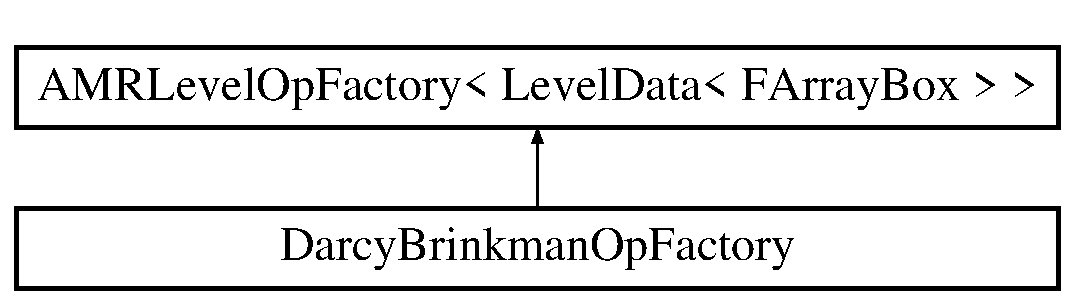
\includegraphics[height=2.000000cm]{class_darcy_brinkman_op_factory}
\end{center}
\end{figure}
\subsection*{Public Member Functions}
\begin{DoxyCompactItemize}
\item 
\hypertarget{class_darcy_brinkman_op_factory_a33cfe1c1920f58a73f46b7dc5b9b0f3b}{\hyperlink{class_darcy_brinkman_op_factory_a33cfe1c1920f58a73f46b7dc5b9b0f3b}{Darcy\-Brinkman\-Op\-Factory} ()}\label{class_darcy_brinkman_op_factory_a33cfe1c1920f58a73f46b7dc5b9b0f3b}

\begin{DoxyCompactList}\small\item\em Default constructor. \end{DoxyCompactList}\item 
void \hyperlink{class_darcy_brinkman_op_factory_adffcc15076241ed69d214197b2c21433}{define} (const Problem\-Domain \&a\-\_\-coarse\-Domain, const Vector$<$ Disjoint\-Box\-Layout $>$ \&a\-\_\-grids, const Vector$<$ int $>$ \&a\-\_\-ref\-Ratios, const Real \&a\-\_\-coarsedx, B\-C\-Holder a\-\_\-bc, const Real \&a\-\_\-alpha, Vector$<$ Ref\-Counted\-Ptr$<$ Level\-Data$<$ F\-Array\-Box $>$ $>$ $>$ \&a\-\_\-a\-Coef, const Real \&a\-\_\-beta, Vector$<$ Ref\-Counted\-Ptr$<$ Level\-Data$<$ Flux\-Box $>$ $>$ $>$ \&a\-\_\-b\-Coef, Vector$<$ Ref\-Counted\-Ptr$<$ Level\-Data$<$ F\-Array\-Box $>$ $>$ $>$ \&a\-\_\-c\-Coef)
\begin{DoxyCompactList}\small\item\em define method \end{DoxyCompactList}\item 
void \hyperlink{class_darcy_brinkman_op_factory_a128c500e2c129aa3bc6ba7e20bf23cf1}{define} (const Problem\-Domain \&a\-\_\-coarse\-Domain, const Vector$<$ Disjoint\-Box\-Layout $>$ \&a\-\_\-grids, const Vector$<$ int $>$ \&a\-\_\-ref\-Ratios, const Real \&a\-\_\-coarsedx, B\-C\-Holder a\-\_\-bc, const Int\-Vect \&a\-\_\-ghost\-Vect)
\item 
\hypertarget{class_darcy_brinkman_op_factory_a6b5e609db52c2363aa015eb0b811d98d}{virtual M\-G\-Level\-Op$<$ Level\-Data\\*
$<$ F\-Array\-Box $>$ $>$ $\ast$ \hyperlink{class_darcy_brinkman_op_factory_a6b5e609db52c2363aa015eb0b811d98d}{M\-Gnew\-Op} (const Problem\-Domain \&a\-\_\-\-Fineindex\-Space, int a\-\_\-depth, bool a\-\_\-homo\-Only=true)}\label{class_darcy_brinkman_op_factory_a6b5e609db52c2363aa015eb0b811d98d}

\begin{DoxyCompactList}\small\item\em make new M\-G\-Level\-Op \end{DoxyCompactList}\item 
\hypertarget{class_darcy_brinkman_op_factory_a82a0943e3ec0acaa1954c1f4c3e3bfa7}{virtual A\-M\-R\-Level\-Op$<$ Level\-Data\\*
$<$ F\-Array\-Box $>$ $>$ $\ast$ \hyperlink{class_darcy_brinkman_op_factory_a82a0943e3ec0acaa1954c1f4c3e3bfa7}{A\-M\-Rnew\-Op} (const Problem\-Domain \&a\-\_\-index\-Space)}\label{class_darcy_brinkman_op_factory_a82a0943e3ec0acaa1954c1f4c3e3bfa7}

\begin{DoxyCompactList}\small\item\em make new A\-M\-R\-Level\-Op \end{DoxyCompactList}\item 
\hypertarget{class_darcy_brinkman_op_factory_a416f30542290000a01ccf209fabd5646}{virtual int \hyperlink{class_darcy_brinkman_op_factory_a416f30542290000a01ccf209fabd5646}{ref\-To\-Finer} (const Problem\-Domain \&a\-\_\-domain) const }\label{class_darcy_brinkman_op_factory_a416f30542290000a01ccf209fabd5646}

\begin{DoxyCompactList}\small\item\em ref ratio to next finer level \end{DoxyCompactList}\end{DoxyCompactItemize}
\subsection*{Public Attributes}
\begin{DoxyCompactItemize}
\item 
\hypertarget{class_darcy_brinkman_op_factory_a02ce1a05ae4fba39abdc0c37ebd8afd8}{int \hyperlink{class_darcy_brinkman_op_factory_a02ce1a05ae4fba39abdc0c37ebd8afd8}{m\-\_\-coefficient\-\_\-average\-\_\-type}}\label{class_darcy_brinkman_op_factory_a02ce1a05ae4fba39abdc0c37ebd8afd8}

\begin{DoxyCompactList}\small\item\em coefficient averaging method \end{DoxyCompactList}\end{DoxyCompactItemize}


\subsection{Detailed Description}
Factory to create \hyperlink{class_darcy_brinkman_op}{Darcy\-Brinkman\-Op}. 

Factory to create Darcy\-Brinkman\-Ops 

\subsection{Member Function Documentation}
\hypertarget{class_darcy_brinkman_op_factory_adffcc15076241ed69d214197b2c21433}{\index{Darcy\-Brinkman\-Op\-Factory@{Darcy\-Brinkman\-Op\-Factory}!define@{define}}
\index{define@{define}!DarcyBrinkmanOpFactory@{Darcy\-Brinkman\-Op\-Factory}}
\subsubsection[{define}]{\setlength{\rightskip}{0pt plus 5cm}void Darcy\-Brinkman\-Op\-Factory\-::define (
\begin{DoxyParamCaption}
\item[{const Problem\-Domain \&}]{a\-\_\-coarse\-Domain, }
\item[{const Vector$<$ Disjoint\-Box\-Layout $>$ \&}]{a\-\_\-grids, }
\item[{const Vector$<$ int $>$ \&}]{a\-\_\-ref\-Ratios, }
\item[{const Real \&}]{a\-\_\-coarsedx, }
\item[{B\-C\-Holder}]{a\-\_\-bc, }
\item[{const Real \&}]{a\-\_\-alpha, }
\item[{Vector$<$ Ref\-Counted\-Ptr$<$ Level\-Data$<$ F\-Array\-Box $>$ $>$ $>$ \&}]{a\-\_\-a\-Coef, }
\item[{const Real \&}]{a\-\_\-beta, }
\item[{Vector$<$ Ref\-Counted\-Ptr$<$ Level\-Data$<$ Flux\-Box $>$ $>$ $>$ \&}]{a\-\_\-b\-Coef, }
\item[{Vector$<$ Ref\-Counted\-Ptr$<$ Level\-Data$<$ F\-Array\-Box $>$ $>$ $>$ \&}]{a\-\_\-c\-Coef}
\end{DoxyParamCaption}
)}}\label{class_darcy_brinkman_op_factory_adffcc15076241ed69d214197b2c21433}


define method 

a\-\_\-coarse\-Domain is the domain at the coarsest level. a\-\_\-grids is the A\-M\-R hierarchy. a\-\_\-ref\-Ratios are the refinement ratios between levels. The ratio lives with the coarser level so a\-\_\-ref\-Ratios\mbox{[}ilev\mbox{]} is the ratio between ilev and ilev+1 a\-\_\-coarse\-Dx is the grid spacing at the coarsest level. a\-\_\-bc holds the boundary conditions. a\-\_\-alpha is the identity constant coefficient a\-\_\-beta is the laplacian constant coefficient. a\-\_\-a\-Coef is the identity spatially varying coefficient a\-\_\-b\-Coef is the laplacian spatially varying coefficient. \hypertarget{class_darcy_brinkman_op_factory_a128c500e2c129aa3bc6ba7e20bf23cf1}{\index{Darcy\-Brinkman\-Op\-Factory@{Darcy\-Brinkman\-Op\-Factory}!define@{define}}
\index{define@{define}!DarcyBrinkmanOpFactory@{Darcy\-Brinkman\-Op\-Factory}}
\subsubsection[{define}]{\setlength{\rightskip}{0pt plus 5cm}void Darcy\-Brinkman\-Op\-Factory\-::define (
\begin{DoxyParamCaption}
\item[{const Problem\-Domain \&}]{a\-\_\-coarse\-Domain, }
\item[{const Vector$<$ Disjoint\-Box\-Layout $>$ \&}]{a\-\_\-grids, }
\item[{const Vector$<$ int $>$ \&}]{a\-\_\-ref\-Ratios, }
\item[{const Real \&}]{a\-\_\-coarsedx, }
\item[{B\-C\-Holder}]{a\-\_\-bc, }
\item[{const Int\-Vect \&}]{a\-\_\-ghost\-Vect}
\end{DoxyParamCaption}
)}}\label{class_darcy_brinkman_op_factory_a128c500e2c129aa3bc6ba7e20bf23cf1}
Defines a factory for \hyperlink{class_darcy_brinkman_op}{Darcy\-Brinkman\-Op} which allows the operators to allocate their own coefficient data. $\alpha$ and $\beta$ coefficients are initialized to 1. 
\begin{DoxyParams}{Parameters}
{\em a\-\_\-coarse\-Domain} & The domain at the coarsest level. \\
\hline
{\em a\-\_\-grids} & The disjoint box layouts for the various refinement levels. \\
\hline
{\em a\-\_\-ref\-Ratios} & The refinement ratios between levels. \\
\hline
{\em a\-\_\-coarsedx} & The grid spacing at the coarsest level. \\
\hline
{\em a\-\_\-bc} & The boundary condition imposed on the solution. \\
\hline
{\em a\-\_\-ghost\-Vect} & The ghost stencil to use in the created coefficient data. \\
\hline
\end{DoxyParams}


The documentation for this class was generated from the following files\-:\begin{DoxyCompactItemize}
\item 
/home/parkinsonjl/mushy-\/layer/src/Darcy\-Brinkman\-Op.\-H\item 
/home/parkinsonjl/mushy-\/layer/src/Darcy\-Brinkman\-Op.\-cpp\end{DoxyCompactItemize}

\hypertarget{class_diagnostics}{\section{Diagnostics Class Reference}
\label{class_diagnostics}\index{Diagnostics@{Diagnostics}}
}


Class to contain diagnostics.  




{\ttfamily \#include $<$Diagnostics.\-h$>$}

\subsection*{Public Types}
\begin{DoxyCompactItemize}
\item 
enum \hyperlink{class_diagnostics_a773b8651afdbc8f9d6106c01a093814f}{diagnostic\-Names} \{ \\*
{\bfseries m\-\_\-time}, 
{\bfseries m\-\_\-dt}, 
{\bfseries m\-\_\-average\-Vertical\-Salt\-Flux}, 
{\bfseries m\-\_\-\-L2\-Fs\-Vert\-Diffusion}, 
\\*
{\bfseries m\-\_\-\-L2\-Fs\-Vert\-Fluid}, 
{\bfseries m\-\_\-\-L2\-Fs\-Vert\-Frame}, 
{\bfseries m\-\_\-\-L1\-Fs\-Vert\-Diffusion}, 
{\bfseries m\-\_\-\-L1\-Fs\-Vert\-Fluid}, 
\\*
{\bfseries m\-\_\-\-L1\-Fs\-Vert\-Frame}, 
{\bfseries m\-\_\-\-L0\-Fs\-Vert\-Diffusion}, 
{\bfseries m\-\_\-\-L0\-Fs\-Vert\-Fluid}, 
{\bfseries m\-\_\-\-L0\-Fs\-Vert\-Frame}, 
\\*
{\bfseries m\-\_\-solute\-Flux\-Top}, 
{\bfseries m\-\_\-solute\-Flux\-Bottom}, 
{\bfseries m\-\_\-solute\-Flux\-Sponge}, 
{\bfseries m\-\_\-heat\-Flux\-Bottom}, 
\\*
{\bfseries m\-\_\-heat\-Flux\-Top}, 
{\bfseries m\-\_\-d\-Udt}, 
{\bfseries m\-\_\-d\-Sdt}, 
{\bfseries m\-\_\-d\-Tdt}, 
\\*
{\bfseries m\-\_\-chimney\-Spacing}, 
{\bfseries m\-\_\-chimney\-Width}, 
{\bfseries m\-\_\-\-Horiz\-Av\-Salinity0}, 
{\bfseries m\-\_\-\-Horiz\-Av\-Salinity20}, 
\\*
{\bfseries m\-\_\-\-Horiz\-Av\-Salinity40}, 
{\bfseries m\-\_\-\-Horiz\-Av\-Salinity60}, 
{\bfseries m\-\_\-av\-Salinity}, 
{\bfseries m\-\_\-mush\-Depth}, 
\\*
{\bfseries m\-\_\-\-Nu}, 
{\bfseries m\-\_\-heat\-Flux\-Abs\-Mismatch}, 
{\bfseries m\-\_\-salt\-Flux\-Abs\-Mismatch}, 
{\bfseries m\-\_\-heat\-Flux\-Rel\-Mismatch}, 
\\*
{\bfseries m\-\_\-salt\-Flux\-Rel\-Mismatch}, 
{\bfseries m\-\_\-max\-Lambda}, 
{\bfseries m\-\_\-sum\-Lambda}, 
{\bfseries m\-\_\-max\-Vel}, 
\\*
{\bfseries m\-\_\-num\-Diagnostics}
 \}
\begin{DoxyCompactList}\small\item\em Different diagnostics we consider. \end{DoxyCompactList}\end{DoxyCompactItemize}
\subsection*{Public Member Functions}
\begin{DoxyCompactItemize}
\item 
\hypertarget{class_diagnostics_a24c4f22a9628a083b82a194089cfdd19}{\hyperlink{class_diagnostics_a24c4f22a9628a083b82a194089cfdd19}{Diagnostics} ()}\label{class_diagnostics_a24c4f22a9628a083b82a194089cfdd19}

\begin{DoxyCompactList}\small\item\em Default constructore. \end{DoxyCompactList}\item 
\hypertarget{class_diagnostics_a33a91e98836bc1c3bf022c09a97b5e51}{void \hyperlink{class_diagnostics_a33a91e98836bc1c3bf022c09a97b5e51}{define} (Real a\-\_\-moving\-Average\-Timescale, int a\-\_\-verbosity, Real a\-\_\-conv\-Crit)}\label{class_diagnostics_a33a91e98836bc1c3bf022c09a97b5e51}

\begin{DoxyCompactList}\small\item\em Define object. \end{DoxyCompactList}\item 
\hypertarget{class_diagnostics_a4051c6c9cfa8a2c0fa30ee2bdd3ff8b5}{void \hyperlink{class_diagnostics_a4051c6c9cfa8a2c0fa30ee2bdd3ff8b5}{add\-Diagnostic} (int a\-\_\-diagnostic, Real a\-\_\-time, Real value)}\label{class_diagnostics_a4051c6c9cfa8a2c0fa30ee2bdd3ff8b5}

\begin{DoxyCompactList}\small\item\em Add a diagnostic. \end{DoxyCompactList}\item 
\hypertarget{class_diagnostics_adbcc14b64242b09e780950d8814608db}{Real \hyperlink{class_diagnostics_adbcc14b64242b09e780950d8814608db}{get\-Diagnostic} (int a\-\_\-diagnostic, Real a\-\_\-time, int timestep\-Offset=0)}\label{class_diagnostics_adbcc14b64242b09e780950d8814608db}

\begin{DoxyCompactList}\small\item\em Get the value of a diagnostic, $ \alpha $. \end{DoxyCompactList}\item 
\hypertarget{class_diagnostics_a8213d3b6dc239506777f7161a07b5635}{Real \hyperlink{class_diagnostics_a8213d3b6dc239506777f7161a07b5635}{get\-Moving\-Average} (int a\-\_\-diagnostic, Real a\-\_\-end\-Time, Real a\-\_\-time\-Span)}\label{class_diagnostics_a8213d3b6dc239506777f7161a07b5635}

\begin{DoxyCompactList}\small\item\em Get the moving average of a diagnostic. \end{DoxyCompactList}\item 
\hypertarget{class_diagnostics_a7b5123f8f4ba2972d02f09026b7532c9}{Real \hyperlink{class_diagnostics_a7b5123f8f4ba2972d02f09026b7532c9}{get\-Rate\-Of\-Change} (int a\-\_\-diagnostic, Real a\-\_\-end\-Time, Real a\-\_\-dt)}\label{class_diagnostics_a7b5123f8f4ba2972d02f09026b7532c9}

\begin{DoxyCompactList}\small\item\em Get $ \frac{d \alpha}{d t} $. \end{DoxyCompactList}\item 
\hypertarget{class_diagnostics_a1785a5913fda81eb98c9f72a44aca154}{Real \hyperlink{class_diagnostics_a1785a5913fda81eb98c9f72a44aca154}{get\-Second\-Rate\-Of\-Change} (int a\-\_\-diagnostic, Real a\-\_\-end\-Time, Real a\-\_\-dt)}\label{class_diagnostics_a1785a5913fda81eb98c9f72a44aca154}

\begin{DoxyCompactList}\small\item\em Calculate $ \frac{d^2 \alpha}{dt^2} $. \end{DoxyCompactList}\item 
\hypertarget{class_diagnostics_a26cd9476e6f736d2fead8380db0f9fa2}{bool \hyperlink{class_diagnostics_a26cd9476e6f736d2fead8380db0f9fa2}{moving\-Average\-Has\-Converged} (int a\-\_\-diagnostic, Real m\-\_\-time, Real a\-\_\-dt)}\label{class_diagnostics_a26cd9476e6f736d2fead8380db0f9fa2}

\begin{DoxyCompactList}\small\item\em Determine if the moving average has reached steady state. \end{DoxyCompactList}\item 
\hypertarget{class_diagnostics_a2868f16188ebe067533afd6c0a27ff6a}{void {\bfseries print\-Header} ()}\label{class_diagnostics_a2868f16188ebe067533afd6c0a27ff6a}

\item 
\hypertarget{class_diagnostics_a69849023434b32047f39b51e0630f568}{void {\bfseries print\-Header} (std\-::ofstream \&a\-\_\-file)}\label{class_diagnostics_a69849023434b32047f39b51e0630f568}

\item 
\hypertarget{class_diagnostics_acd87da429ff720d80cbb2e82431fadb7}{void {\bfseries print\-Diagnostics} (Real a\-\_\-time)}\label{class_diagnostics_acd87da429ff720d80cbb2e82431fadb7}

\item 
\hypertarget{class_diagnostics_a510534ea0fa2b5e49f9f0aec1d7f8693}{void {\bfseries print\-Diagnostics} (Real a\-\_\-time, std\-::ofstream \&a\-\_\-file)}\label{class_diagnostics_a510534ea0fa2b5e49f9f0aec1d7f8693}

\end{DoxyCompactItemize}


\subsection{Detailed Description}
Class to contain diagnostics. 

This class manages various diagnostics that we want to track during simulations 

The documentation for this class was generated from the following files\-:\begin{DoxyCompactItemize}
\item 
/home/parkinsonjl/mushy-\/layer/src/Diagnostics.\-h\item 
/home/parkinsonjl/mushy-\/layer/src/Diagnostics.\-cpp\end{DoxyCompactItemize}

\hypertarget{class_divergence}{\section{Divergence Class Reference}
\label{class_divergence}\index{Divergence@{Divergence}}
}


Class to encapsulate \hyperlink{class_divergence}{Divergence} functions.  




{\ttfamily \#include $<$Divergence.\-H$>$}

\subsection*{Static Public Member Functions}
\begin{DoxyCompactItemize}
\item 
static void \hyperlink{class_divergence_a85ddcbfb1ed4cd7e6624c33d0bd918f3}{level\-Divergence\-C\-C} (Level\-Data$<$ F\-Array\-Box $>$ \&a\-\_\-div, Level\-Data$<$ F\-Array\-Box $>$ \&a\-\_\-u, Level\-Data$<$ F\-Array\-Box $>$ $\ast$a\-\_\-u\-Crse\-Ptr, const Real a\-\_\-dx, const int a\-\_\-n\-Ref\-Crse, const Problem\-Domain \&a\-\_\-d\-Problem, const bool a\-\_\-quad\-Interp)
\item 
static void \hyperlink{class_divergence_a832809fde8a4344564e82a2a4881dccb}{level\-Divergence\-C\-C} (Level\-Data$<$ F\-Array\-Box $>$ \&a\-\_\-div, Level\-Data$<$ F\-Array\-Box $>$ \&a\-\_\-u, Level\-Data$<$ F\-Array\-Box $>$ $\ast$a\-\_\-u\-Crse\-Ptr, const Real a\-\_\-dx, const int a\-\_\-n\-Ref\-Crse, const Box \&a\-\_\-d\-Problem, const bool a\-\_\-quad\-Interp)
\item 
static void \hyperlink{class_divergence_a8714fec933884a4b9e6f8173e22574e3}{level\-Divergence\-C\-C} (Level\-Data$<$ F\-Array\-Box $>$ \&a\-\_\-div, Level\-Data$<$ F\-Array\-Box $>$ \&a\-\_\-u, Level\-Data$<$ F\-Array\-Box $>$ $\ast$a\-\_\-u\-Crse\-Ptr, const Real a\-\_\-dx, const bool a\-\_\-quad\-Interp, Quad\-C\-F\-Interp \&a\-\_\-cf\-Interp)
\item 
\hypertarget{class_divergence_ae2ca2377231f1c6a272151d3ffe95432}{static void \hyperlink{class_divergence_ae2ca2377231f1c6a272151d3ffe95432}{level\-Divergence\-C\-C} (Level\-Data$<$ F\-Array\-Box $>$ \&a\-\_\-div, Level\-Data$<$ F\-Array\-Box $>$ \&a\-\_\-u, const Real a\-\_\-dx)}\label{class_divergence_ae2ca2377231f1c6a272151d3ffe95432}

\begin{DoxyCompactList}\small\item\em Version for a single level, assumes B\-Cs all set. \end{DoxyCompactList}\item 
static void \hyperlink{class_divergence_a77ec6a5b421cc2360223b7b0879786e8}{level\-Divergence\-C\-C\-New} (Level\-Data$<$ F\-Array\-Box $>$ \&a\-\_\-div, Level\-Data$<$ F\-Array\-Box $>$ \&a\-\_\-u, Level\-Data$<$ F\-Array\-Box $>$ $\ast$a\-\_\-u\-Crse\-Ptr, const Real a\-\_\-dx, const bool a\-\_\-quad\-Interp, Quad\-C\-F\-Interp \&a\-\_\-cf\-Interp)
\item 
static void \hyperlink{class_divergence_af3bff43b62b95d79fcd50484019e3e41}{comp\-Divergence\-C\-C} (Level\-Data$<$ F\-Array\-Box $>$ \&a\-\_\-div, Level\-Data$<$ F\-Array\-Box $>$ \&a\-\_\-u, Level\-Data$<$ F\-Array\-Box $>$ $\ast$a\-\_\-u\-Crse\-Ptr, Level\-Data$<$ F\-Array\-Box $>$ $\ast$a\-\_\-u\-Fine\-Ptr, const Real a\-\_\-dx, const int a\-\_\-n\-Ref\-Crse, const int a\-\_\-n\-Ref\-Fine, const Problem\-Domain \&a\-\_\-d\-Problem, const bool a\-\_\-quad\-Interp)
\item 
static void \hyperlink{class_divergence_ad1d85e2db60cacec07a004c9d0b19b24}{comp\-Divergence\-C\-C} (Level\-Data$<$ F\-Array\-Box $>$ \&a\-\_\-div, Level\-Data$<$ F\-Array\-Box $>$ \&a\-\_\-u, Level\-Data$<$ F\-Array\-Box $>$ $\ast$a\-\_\-u\-Crse\-Ptr, Level\-Data$<$ F\-Array\-Box $>$ $\ast$a\-\_\-u\-Fine\-Ptr, const Real a\-\_\-dx, const int a\-\_\-n\-Ref\-Crse, const int a\-\_\-n\-Ref\-Fine, const Box \&a\-\_\-d\-Problem, const bool a\-\_\-quad\-Interp)
\item 
static void \hyperlink{class_divergence_a4bafaf6a0fee4270b05bfb1b31c915ed}{comp\-Divergence\-C\-C} (Level\-Data$<$ F\-Array\-Box $>$ \&a\-\_\-div, Level\-Data$<$ F\-Array\-Box $>$ \&a\-\_\-u, Level\-Data$<$ F\-Array\-Box $>$ $\ast$a\-\_\-u\-Crse\-Ptr, Level\-Data$<$ F\-Array\-Box $>$ $\ast$a\-\_\-u\-Fine\-Ptr, const Real a\-\_\-dx, const int a\-\_\-n\-Ref\-Fine, const int a\-\_\-n\-Ref\-Crse, const Problem\-Domain \&a\-\_\-d\-Problem, const bool a\-\_\-quad\-Interp, Level\-Flux\-Register $\ast$a\-\_\-flux\-Reg\-Fine\-Ptr, Quad\-C\-F\-Interp \&a\-\_\-cf\-Interp\-Crse, Quad\-C\-F\-Interp \&a\-\_\-cf\-Interp\-Fine)
\item 
static void \hyperlink{class_divergence_ab20b13344306e041cbf99e4234a46244}{comp\-Divergence\-C\-C} (Level\-Data$<$ F\-Array\-Box $>$ \&a\-\_\-div, Level\-Data$<$ F\-Array\-Box $>$ \&a\-\_\-u, Level\-Data$<$ F\-Array\-Box $>$ $\ast$a\-\_\-u\-Crse\-Ptr, Level\-Data$<$ F\-Array\-Box $>$ $\ast$a\-\_\-u\-Fine\-Ptr, const Real a\-\_\-dx, const int a\-\_\-n\-Ref\-Fine, const int a\-\_\-n\-Ref\-Crse, const Box \&a\-\_\-d\-Problem, const bool a\-\_\-quad\-Interp, Level\-Flux\-Register $\ast$a\-\_\-flux\-Reg\-Fine\-Ptr, Quad\-C\-F\-Interp \&a\-\_\-cf\-Interp\-Crse, Quad\-C\-F\-Interp \&a\-\_\-cf\-Interp\-Fine)
\item 
static void \hyperlink{class_divergence_a9004d4f62127cfaecab354769b4fcd58}{level\-Divergence\-M\-A\-C} (Level\-Data$<$ F\-Array\-Box $>$ \&a\-\_\-div, const Level\-Data$<$ Flux\-Box $>$ \&a\-\_\-u\-Edge, const Real a\-\_\-dx)
\item 
static void \hyperlink{class_divergence_a6e222e89a13a45cbc06f380302aebf13}{level\-Divergence\-M\-A\-C\-Multi\-Comp} (Level\-Data$<$ F\-Array\-Box $>$ \&a\-\_\-div, const Level\-Data$<$ Flux\-Box $>$ \&a\-\_\-u\-Edge, const Real a\-\_\-dx)
\begin{DoxyCompactList}\small\item\em Computes divergence of fields containing multiple components. \end{DoxyCompactList}\item 
\hypertarget{class_divergence_acc40ffe25f3b5a7eeb35cfab48873180}{static void \hyperlink{class_divergence_acc40ffe25f3b5a7eeb35cfab48873180}{simple\-Divergence\-M\-A\-C} (F\-Array\-Box \&a\-\_\-div, const Flux\-Box \&a\-\_\-u\-Edge, const Real a\-\_\-dx)}\label{class_divergence_acc40ffe25f3b5a7eeb35cfab48873180}

\begin{DoxyCompactList}\small\item\em really basic single-\/fab M\-A\-C divergence \end{DoxyCompactList}\item 
static void \hyperlink{class_divergence_acd62afebbe823676309ba7301578ea96}{comp\-Divergence\-M\-A\-C} (Level\-Data$<$ F\-Array\-Box $>$ \&a\-\_\-div, Level\-Data$<$ Flux\-Box $>$ \&a\-\_\-u\-Edge, Level\-Data$<$ Flux\-Box $>$ $\ast$a\-\_\-u\-Edge\-Fine\-Ptr, const Real a\-\_\-dx, const Real $\ast$a\-\_\-dx\-Fine, const int a\-\_\-n\-Ref\-Fine, const Problem\-Domain \&a\-\_\-d\-Problem)
\item 
static void \hyperlink{class_divergence_ab223946c8b00bee70b0f73530ef274fe}{comp\-Divergence\-M\-A\-C} (Level\-Data$<$ F\-Array\-Box $>$ \&a\-\_\-div, Level\-Data$<$ Flux\-Box $>$ \&a\-\_\-u\-Edge, Level\-Data$<$ Flux\-Box $>$ $\ast$a\-\_\-u\-Edge\-Fine\-Ptr, const Real a\-\_\-dx, const Real $\ast$a\-\_\-dx\-Fine, const int a\-\_\-n\-Ref\-Fine, const Box \&a\-\_\-d\-Problem)
\item 
static void \hyperlink{class_divergence_a7ea9ccc4a12abac5f0141e67c69f9c0f}{comp\-Divergence\-M\-A\-C} (Level\-Data$<$ F\-Array\-Box $>$ \&a\-\_\-div, Level\-Data$<$ Flux\-Box $>$ \&a\-\_\-u\-Edge, Level\-Data$<$ Flux\-Box $>$ $\ast$a\-\_\-u\-Edge\-Fine\-Ptr, Level\-Flux\-Register $\ast$a\-\_\-flux\-Reg\-Ptr, const Real a\-\_\-dx, const Real $\ast$a\-\_\-dx\-Fine, const int a\-\_\-n\-Refine, const Problem\-Domain \&a\-\_\-d\-Problem)
\item 
static void \hyperlink{class_divergence_a6edc8c244f67ac7fcaf54386a1fed40b}{comp\-Divergence\-M\-A\-C} (Level\-Data$<$ F\-Array\-Box $>$ \&a\-\_\-div, Level\-Data$<$ Flux\-Box $>$ \&a\-\_\-u\-Edge, Level\-Data$<$ Flux\-Box $>$ $\ast$a\-\_\-u\-Edge\-Fine\-Ptr, Level\-Flux\-Register $\ast$a\-\_\-flux\-Reg\-Ptr, const Real a\-\_\-dx, const Real $\ast$a\-\_\-dx\-Fine, const int a\-\_\-n\-Refine, const Box \&a\-\_\-d\-Problem)
\end{DoxyCompactItemize}


\subsection{Detailed Description}
Class to encapsulate \hyperlink{class_divergence}{Divergence} functions. 

\subsection{Member Function Documentation}
\hypertarget{class_divergence_af3bff43b62b95d79fcd50484019e3e41}{\index{Divergence@{Divergence}!comp\-Divergence\-C\-C@{comp\-Divergence\-C\-C}}
\index{comp\-Divergence\-C\-C@{comp\-Divergence\-C\-C}!Divergence@{Divergence}}
\subsubsection[{comp\-Divergence\-C\-C}]{\setlength{\rightskip}{0pt plus 5cm}void Divergence\-::comp\-Divergence\-C\-C (
\begin{DoxyParamCaption}
\item[{Level\-Data$<$ F\-Array\-Box $>$ \&}]{a\-\_\-div, }
\item[{Level\-Data$<$ F\-Array\-Box $>$ \&}]{a\-\_\-u, }
\item[{Level\-Data$<$ F\-Array\-Box $>$ $\ast$}]{a\-\_\-u\-Crse\-Ptr, }
\item[{Level\-Data$<$ F\-Array\-Box $>$ $\ast$}]{a\-\_\-u\-Fine\-Ptr, }
\item[{const Real}]{a\-\_\-dx, }
\item[{const int}]{a\-\_\-n\-Ref\-Crse, }
\item[{const int}]{a\-\_\-n\-Ref\-Fine, }
\item[{const Problem\-Domain \&}]{a\-\_\-d\-Problem, }
\item[{const bool}]{a\-\_\-quad\-Interp}
\end{DoxyParamCaption}
)\hspace{0.3cm}{\ttfamily [static]}}}\label{class_divergence_af3bff43b62b95d79fcd50484019e3e41}
computes cell-\/centered composite-\/operator divergence of cell-\/centered vector field u; uses same coarse-\/fine B\-C's as level\-Divergence\-C\-C -- if u\-Fine != N\-U\-L\-L, also does flux-\/matching B\-C with finer level u\-Fine, using same coarse-\/fine B\-C's as used for coarse level B\-C. N\-O\-T\-E -\/ this expects 1 (one) ghost cell! \hypertarget{class_divergence_ad1d85e2db60cacec07a004c9d0b19b24}{\index{Divergence@{Divergence}!comp\-Divergence\-C\-C@{comp\-Divergence\-C\-C}}
\index{comp\-Divergence\-C\-C@{comp\-Divergence\-C\-C}!Divergence@{Divergence}}
\subsubsection[{comp\-Divergence\-C\-C}]{\setlength{\rightskip}{0pt plus 5cm}void Divergence\-::comp\-Divergence\-C\-C (
\begin{DoxyParamCaption}
\item[{Level\-Data$<$ F\-Array\-Box $>$ \&}]{a\-\_\-div, }
\item[{Level\-Data$<$ F\-Array\-Box $>$ \&}]{a\-\_\-u, }
\item[{Level\-Data$<$ F\-Array\-Box $>$ $\ast$}]{a\-\_\-u\-Crse\-Ptr, }
\item[{Level\-Data$<$ F\-Array\-Box $>$ $\ast$}]{a\-\_\-u\-Fine\-Ptr, }
\item[{const Real}]{a\-\_\-dx, }
\item[{const int}]{a\-\_\-n\-Ref\-Crse, }
\item[{const int}]{a\-\_\-n\-Ref\-Fine, }
\item[{const Box \&}]{a\-\_\-d\-Problem, }
\item[{const bool}]{a\-\_\-quad\-Interp}
\end{DoxyParamCaption}
)\hspace{0.3cm}{\ttfamily [static]}}}\label{class_divergence_ad1d85e2db60cacec07a004c9d0b19b24}
computes cell-\/centered composite-\/operator divergence of cell-\/centered vector field u; uses same coarse-\/fine B\-C's as level\-Divergence\-C\-C -- if u\-Fine != N\-U\-L\-L, also does flux-\/matching B\-C with finer level u\-Fine, using same coarse-\/fine B\-C's as used for coarse level B\-C. This (deprecated) interface uses a Box instead of a Problem\-Domain \hypertarget{class_divergence_a4bafaf6a0fee4270b05bfb1b31c915ed}{\index{Divergence@{Divergence}!comp\-Divergence\-C\-C@{comp\-Divergence\-C\-C}}
\index{comp\-Divergence\-C\-C@{comp\-Divergence\-C\-C}!Divergence@{Divergence}}
\subsubsection[{comp\-Divergence\-C\-C}]{\setlength{\rightskip}{0pt plus 5cm}void Divergence\-::comp\-Divergence\-C\-C (
\begin{DoxyParamCaption}
\item[{Level\-Data$<$ F\-Array\-Box $>$ \&}]{a\-\_\-div, }
\item[{Level\-Data$<$ F\-Array\-Box $>$ \&}]{a\-\_\-u, }
\item[{Level\-Data$<$ F\-Array\-Box $>$ $\ast$}]{a\-\_\-u\-Crse\-Ptr, }
\item[{Level\-Data$<$ F\-Array\-Box $>$ $\ast$}]{a\-\_\-u\-Fine\-Ptr, }
\item[{const Real}]{a\-\_\-dx, }
\item[{const int}]{a\-\_\-n\-Ref\-Fine, }
\item[{const int}]{a\-\_\-n\-Ref\-Crse, }
\item[{const Problem\-Domain \&}]{a\-\_\-d\-Problem, }
\item[{const bool}]{a\-\_\-quad\-Interp, }
\item[{Level\-Flux\-Register $\ast$}]{a\-\_\-flux\-Reg\-Fine\-Ptr, }
\item[{Quad\-C\-F\-Interp \&}]{a\-\_\-cf\-Interp\-Crse, }
\item[{Quad\-C\-F\-Interp \&}]{a\-\_\-cf\-Interp\-Fine}
\end{DoxyParamCaption}
)\hspace{0.3cm}{\ttfamily [static]}}}\label{class_divergence_a4bafaf6a0fee4270b05bfb1b31c915ed}
computes cell-\/centered composite-\/operator divergence of cell-\/centered vector field u; uses same coarse-\/fine B\-C's as level\-Divergence\-C\-C -- if u\-Fine != N\-U\-L\-L, also does flux-\/matching B\-C with finer level u\-Fine, using same coarse-\/fine B\-C's as used for coarse level B\-C. In this one, pre-\/allocated Level\-Flux\-Register and Quad\-C\-F\-Interp objects are passed in as an argument (saves allocation inside fn.) \hypertarget{class_divergence_ab20b13344306e041cbf99e4234a46244}{\index{Divergence@{Divergence}!comp\-Divergence\-C\-C@{comp\-Divergence\-C\-C}}
\index{comp\-Divergence\-C\-C@{comp\-Divergence\-C\-C}!Divergence@{Divergence}}
\subsubsection[{comp\-Divergence\-C\-C}]{\setlength{\rightskip}{0pt plus 5cm}void Divergence\-::comp\-Divergence\-C\-C (
\begin{DoxyParamCaption}
\item[{Level\-Data$<$ F\-Array\-Box $>$ \&}]{a\-\_\-div, }
\item[{Level\-Data$<$ F\-Array\-Box $>$ \&}]{a\-\_\-u, }
\item[{Level\-Data$<$ F\-Array\-Box $>$ $\ast$}]{a\-\_\-u\-Crse\-Ptr, }
\item[{Level\-Data$<$ F\-Array\-Box $>$ $\ast$}]{a\-\_\-u\-Fine\-Ptr, }
\item[{const Real}]{a\-\_\-dx, }
\item[{const int}]{a\-\_\-n\-Ref\-Fine, }
\item[{const int}]{a\-\_\-n\-Ref\-Crse, }
\item[{const Box \&}]{a\-\_\-d\-Problem, }
\item[{const bool}]{a\-\_\-quad\-Interp, }
\item[{Level\-Flux\-Register $\ast$}]{a\-\_\-flux\-Reg\-Fine\-Ptr, }
\item[{Quad\-C\-F\-Interp \&}]{a\-\_\-cf\-Interp\-Crse, }
\item[{Quad\-C\-F\-Interp \&}]{a\-\_\-cf\-Interp\-Fine}
\end{DoxyParamCaption}
)\hspace{0.3cm}{\ttfamily [static]}}}\label{class_divergence_ab20b13344306e041cbf99e4234a46244}
computes cell-\/centered composite-\/operator divergence of cell-\/centered vector field u; uses same coarse-\/fine B\-C's as level\-Divergence\-C\-C -- if u\-Fine != N\-U\-L\-L, also does flux-\/matching B\-C with finer level u\-Fine, using same coarse-\/fine B\-C's as used for coarse level B\-C. In this one, pre-\/allocated Level\-Flux\-Register and Quad\-C\-F\-Interp objects are passed in as an argument (saves allocation inside fn.) This (deprecated) interface uses a Box instead of a Problem\-Domain. \hypertarget{class_divergence_acd62afebbe823676309ba7301578ea96}{\index{Divergence@{Divergence}!comp\-Divergence\-M\-A\-C@{comp\-Divergence\-M\-A\-C}}
\index{comp\-Divergence\-M\-A\-C@{comp\-Divergence\-M\-A\-C}!Divergence@{Divergence}}
\subsubsection[{comp\-Divergence\-M\-A\-C}]{\setlength{\rightskip}{0pt plus 5cm}void Divergence\-::comp\-Divergence\-M\-A\-C (
\begin{DoxyParamCaption}
\item[{Level\-Data$<$ F\-Array\-Box $>$ \&}]{a\-\_\-div, }
\item[{Level\-Data$<$ Flux\-Box $>$ \&}]{a\-\_\-u\-Edge, }
\item[{Level\-Data$<$ Flux\-Box $>$ $\ast$}]{a\-\_\-u\-Edge\-Fine\-Ptr, }
\item[{const Real}]{a\-\_\-dx, }
\item[{const Real $\ast$}]{a\-\_\-dx\-Fine, }
\item[{const int}]{a\-\_\-n\-Ref\-Fine, }
\item[{const Problem\-Domain \&}]{a\-\_\-d\-Problem}
\end{DoxyParamCaption}
)\hspace{0.3cm}{\ttfamily [static]}}}\label{class_divergence_acd62afebbe823676309ba7301578ea96}
computes composite cell-\/centered divergence of edge-\/centered vector field u\-Edge; if finer level data u\-Edge\-Fine exists, use flux-\/matching condition to compute divergence along coarse-\/fine interface. \hypertarget{class_divergence_ab223946c8b00bee70b0f73530ef274fe}{\index{Divergence@{Divergence}!comp\-Divergence\-M\-A\-C@{comp\-Divergence\-M\-A\-C}}
\index{comp\-Divergence\-M\-A\-C@{comp\-Divergence\-M\-A\-C}!Divergence@{Divergence}}
\subsubsection[{comp\-Divergence\-M\-A\-C}]{\setlength{\rightskip}{0pt plus 5cm}void Divergence\-::comp\-Divergence\-M\-A\-C (
\begin{DoxyParamCaption}
\item[{Level\-Data$<$ F\-Array\-Box $>$ \&}]{a\-\_\-div, }
\item[{Level\-Data$<$ Flux\-Box $>$ \&}]{a\-\_\-u\-Edge, }
\item[{Level\-Data$<$ Flux\-Box $>$ $\ast$}]{a\-\_\-u\-Edge\-Fine\-Ptr, }
\item[{const Real}]{a\-\_\-dx, }
\item[{const Real $\ast$}]{a\-\_\-dx\-Fine, }
\item[{const int}]{a\-\_\-n\-Ref\-Fine, }
\item[{const Box \&}]{a\-\_\-d\-Problem}
\end{DoxyParamCaption}
)\hspace{0.3cm}{\ttfamily [static]}}}\label{class_divergence_ab223946c8b00bee70b0f73530ef274fe}
computes composite cell-\/centered divergence of edge-\/centered vector field u\-Edge; if finer level data u\-Edge\-Fine exists, use flux-\/matching condition to compute divergence along coarse-\/fine interface. This (deprecated) interface uses a Box instead of a Problem\-Domain \hypertarget{class_divergence_a7ea9ccc4a12abac5f0141e67c69f9c0f}{\index{Divergence@{Divergence}!comp\-Divergence\-M\-A\-C@{comp\-Divergence\-M\-A\-C}}
\index{comp\-Divergence\-M\-A\-C@{comp\-Divergence\-M\-A\-C}!Divergence@{Divergence}}
\subsubsection[{comp\-Divergence\-M\-A\-C}]{\setlength{\rightskip}{0pt plus 5cm}void Divergence\-::comp\-Divergence\-M\-A\-C (
\begin{DoxyParamCaption}
\item[{Level\-Data$<$ F\-Array\-Box $>$ \&}]{a\-\_\-div, }
\item[{Level\-Data$<$ Flux\-Box $>$ \&}]{a\-\_\-u\-Edge, }
\item[{Level\-Data$<$ Flux\-Box $>$ $\ast$}]{a\-\_\-u\-Edge\-Fine\-Ptr, }
\item[{Level\-Flux\-Register $\ast$}]{a\-\_\-flux\-Reg\-Ptr, }
\item[{const Real}]{a\-\_\-dx, }
\item[{const Real $\ast$}]{a\-\_\-dx\-Fine, }
\item[{const int}]{a\-\_\-n\-Refine, }
\item[{const Problem\-Domain \&}]{a\-\_\-d\-Problem}
\end{DoxyParamCaption}
)\hspace{0.3cm}{\ttfamily [static]}}}\label{class_divergence_a7ea9ccc4a12abac5f0141e67c69f9c0f}
just like normal comp\-Divergence\-M\-A\-C, but pass in a predefined flux register (more efficient) \hypertarget{class_divergence_a6edc8c244f67ac7fcaf54386a1fed40b}{\index{Divergence@{Divergence}!comp\-Divergence\-M\-A\-C@{comp\-Divergence\-M\-A\-C}}
\index{comp\-Divergence\-M\-A\-C@{comp\-Divergence\-M\-A\-C}!Divergence@{Divergence}}
\subsubsection[{comp\-Divergence\-M\-A\-C}]{\setlength{\rightskip}{0pt plus 5cm}void Divergence\-::comp\-Divergence\-M\-A\-C (
\begin{DoxyParamCaption}
\item[{Level\-Data$<$ F\-Array\-Box $>$ \&}]{a\-\_\-div, }
\item[{Level\-Data$<$ Flux\-Box $>$ \&}]{a\-\_\-u\-Edge, }
\item[{Level\-Data$<$ Flux\-Box $>$ $\ast$}]{a\-\_\-u\-Edge\-Fine\-Ptr, }
\item[{Level\-Flux\-Register $\ast$}]{a\-\_\-flux\-Reg\-Ptr, }
\item[{const Real}]{a\-\_\-dx, }
\item[{const Real $\ast$}]{a\-\_\-dx\-Fine, }
\item[{const int}]{a\-\_\-n\-Refine, }
\item[{const Box \&}]{a\-\_\-d\-Problem}
\end{DoxyParamCaption}
)\hspace{0.3cm}{\ttfamily [static]}}}\label{class_divergence_a6edc8c244f67ac7fcaf54386a1fed40b}
just like normal comp\-Divergence\-M\-A\-C, but pass in a predefined flux register (more efficient). This (deprecated) interface uses a Box instead of a Problem\-Domain. \hypertarget{class_divergence_a85ddcbfb1ed4cd7e6624c33d0bd918f3}{\index{Divergence@{Divergence}!level\-Divergence\-C\-C@{level\-Divergence\-C\-C}}
\index{level\-Divergence\-C\-C@{level\-Divergence\-C\-C}!Divergence@{Divergence}}
\subsubsection[{level\-Divergence\-C\-C}]{\setlength{\rightskip}{0pt plus 5cm}void Divergence\-::level\-Divergence\-C\-C (
\begin{DoxyParamCaption}
\item[{Level\-Data$<$ F\-Array\-Box $>$ \&}]{a\-\_\-div, }
\item[{Level\-Data$<$ F\-Array\-Box $>$ \&}]{a\-\_\-u, }
\item[{Level\-Data$<$ F\-Array\-Box $>$ $\ast$}]{a\-\_\-u\-Crse\-Ptr, }
\item[{const Real}]{a\-\_\-dx, }
\item[{const int}]{a\-\_\-n\-Ref\-Crse, }
\item[{const Problem\-Domain \&}]{a\-\_\-d\-Problem, }
\item[{const bool}]{a\-\_\-quad\-Interp}
\end{DoxyParamCaption}
)\hspace{0.3cm}{\ttfamily [static]}}}\label{class_divergence_a85ddcbfb1ed4cd7e6624c33d0bd918f3}
computes cell-\/centered level-\/operator divergence of cell-\/centered vector field u; if u\-Crse != N\-U\-L\-L, does coarse-\/fine boundary conditions for u -- if quad\-Interp == true, uses quadratic coarse-\/fine boundary conditions, otherwise, use extrap B\-C's \hypertarget{class_divergence_a832809fde8a4344564e82a2a4881dccb}{\index{Divergence@{Divergence}!level\-Divergence\-C\-C@{level\-Divergence\-C\-C}}
\index{level\-Divergence\-C\-C@{level\-Divergence\-C\-C}!Divergence@{Divergence}}
\subsubsection[{level\-Divergence\-C\-C}]{\setlength{\rightskip}{0pt plus 5cm}void Divergence\-::level\-Divergence\-C\-C (
\begin{DoxyParamCaption}
\item[{Level\-Data$<$ F\-Array\-Box $>$ \&}]{a\-\_\-div, }
\item[{Level\-Data$<$ F\-Array\-Box $>$ \&}]{a\-\_\-u, }
\item[{Level\-Data$<$ F\-Array\-Box $>$ $\ast$}]{a\-\_\-u\-Crse\-Ptr, }
\item[{const Real}]{a\-\_\-dx, }
\item[{const int}]{a\-\_\-n\-Ref\-Crse, }
\item[{const Box \&}]{a\-\_\-d\-Problem, }
\item[{const bool}]{a\-\_\-quad\-Interp}
\end{DoxyParamCaption}
)\hspace{0.3cm}{\ttfamily [static]}}}\label{class_divergence_a832809fde8a4344564e82a2a4881dccb}
computes cell-\/centered level-\/operator divergence of cell-\/centered vector field u; if u\-Crse != N\-U\-L\-L, does coarse-\/fine boundary conditions for u -- if quad\-Interp == true, uses quadratic coarse-\/fine boundary conditions, otherwise, use extrap B\-C's. This (deprecated) interface uses a Box instead of a Problem\-Domain. \hypertarget{class_divergence_a8714fec933884a4b9e6f8173e22574e3}{\index{Divergence@{Divergence}!level\-Divergence\-C\-C@{level\-Divergence\-C\-C}}
\index{level\-Divergence\-C\-C@{level\-Divergence\-C\-C}!Divergence@{Divergence}}
\subsubsection[{level\-Divergence\-C\-C}]{\setlength{\rightskip}{0pt plus 5cm}void Divergence\-::level\-Divergence\-C\-C (
\begin{DoxyParamCaption}
\item[{Level\-Data$<$ F\-Array\-Box $>$ \&}]{a\-\_\-div, }
\item[{Level\-Data$<$ F\-Array\-Box $>$ \&}]{a\-\_\-u, }
\item[{Level\-Data$<$ F\-Array\-Box $>$ $\ast$}]{a\-\_\-u\-Crse\-Ptr, }
\item[{const Real}]{a\-\_\-dx, }
\item[{const bool}]{a\-\_\-quad\-Interp, }
\item[{Quad\-C\-F\-Interp \&}]{a\-\_\-cf\-Interp}
\end{DoxyParamCaption}
)\hspace{0.3cm}{\ttfamily [static]}}}\label{class_divergence_a8714fec933884a4b9e6f8173e22574e3}
computes cell-\/centered level-\/operator divergence of cell-\/centered vector field u; if u\-Crse != N\-U\-L\-L, does coarse-\/fine boundary conditions for u -- if quad\-Interp == true, uses quadratic coarse-\/fine boundary conditions, otherwise, use extrap B\-C's. This one takes a pre-\/allocated Quad\-C\-F\-Interp object as an argument \hypertarget{class_divergence_a77ec6a5b421cc2360223b7b0879786e8}{\index{Divergence@{Divergence}!level\-Divergence\-C\-C\-New@{level\-Divergence\-C\-C\-New}}
\index{level\-Divergence\-C\-C\-New@{level\-Divergence\-C\-C\-New}!Divergence@{Divergence}}
\subsubsection[{level\-Divergence\-C\-C\-New}]{\setlength{\rightskip}{0pt plus 5cm}void Divergence\-::level\-Divergence\-C\-C\-New (
\begin{DoxyParamCaption}
\item[{Level\-Data$<$ F\-Array\-Box $>$ \&}]{a\-\_\-div, }
\item[{Level\-Data$<$ F\-Array\-Box $>$ \&}]{a\-\_\-u, }
\item[{Level\-Data$<$ F\-Array\-Box $>$ $\ast$}]{a\-\_\-u\-Crse\-Ptr, }
\item[{const Real}]{a\-\_\-dx, }
\item[{const bool}]{a\-\_\-quad\-Interp, }
\item[{Quad\-C\-F\-Interp \&}]{a\-\_\-cf\-Interp}
\end{DoxyParamCaption}
)\hspace{0.3cm}{\ttfamily [static]}}}\label{class_divergence_a77ec6a5b421cc2360223b7b0879786e8}
New method that uses one sided diffs everywhere for smooth error.

computes cell-\/centered level-\/operator divergence of cell-\/centered vector field u; if u\-Crse != N\-U\-L\-L, does coarse-\/fine boundary conditions for u -- if quad\-Interp == true, uses quadratic coarse-\/fine boundary conditions, otherwise, use extrap B\-C's. This one takes a pre-\/allocated Quad\-C\-F\-Interp object as an argument \hypertarget{class_divergence_a9004d4f62127cfaecab354769b4fcd58}{\index{Divergence@{Divergence}!level\-Divergence\-M\-A\-C@{level\-Divergence\-M\-A\-C}}
\index{level\-Divergence\-M\-A\-C@{level\-Divergence\-M\-A\-C}!Divergence@{Divergence}}
\subsubsection[{level\-Divergence\-M\-A\-C}]{\setlength{\rightskip}{0pt plus 5cm}void Divergence\-::level\-Divergence\-M\-A\-C (
\begin{DoxyParamCaption}
\item[{Level\-Data$<$ F\-Array\-Box $>$ \&}]{a\-\_\-div, }
\item[{const Level\-Data$<$ Flux\-Box $>$ \&}]{a\-\_\-u\-Edge, }
\item[{const Real}]{a\-\_\-dx}
\end{DoxyParamCaption}
)\hspace{0.3cm}{\ttfamily [static]}}}\label{class_divergence_a9004d4f62127cfaecab354769b4fcd58}
computes cell-\/centered level-\/operator divergence of edge-\/centered vector field u\-Edge; assumes all coarse-\/fine B\-C's have already been set. \hypertarget{class_divergence_a6e222e89a13a45cbc06f380302aebf13}{\index{Divergence@{Divergence}!level\-Divergence\-M\-A\-C\-Multi\-Comp@{level\-Divergence\-M\-A\-C\-Multi\-Comp}}
\index{level\-Divergence\-M\-A\-C\-Multi\-Comp@{level\-Divergence\-M\-A\-C\-Multi\-Comp}!Divergence@{Divergence}}
\subsubsection[{level\-Divergence\-M\-A\-C\-Multi\-Comp}]{\setlength{\rightskip}{0pt plus 5cm}void Divergence\-::level\-Divergence\-M\-A\-C\-Multi\-Comp (
\begin{DoxyParamCaption}
\item[{Level\-Data$<$ F\-Array\-Box $>$ \&}]{a\-\_\-div, }
\item[{const Level\-Data$<$ Flux\-Box $>$ \&}]{a\-\_\-u\-Edge, }
\item[{const Real}]{a\-\_\-dx}
\end{DoxyParamCaption}
)\hspace{0.3cm}{\ttfamily [static]}}}\label{class_divergence_a6e222e89a13a45cbc06f380302aebf13}


Computes divergence of fields containing multiple components. 

\&\&Multi component version\&\& computes cell-\/centered level-\/operator divergence of edge-\/centered vector field u\-Edge; assumes all coarse-\/fine B\-C's have already been set. 

The documentation for this class was generated from the following files\-:\begin{DoxyCompactItemize}
\item 
/home/parkinsonjl/mushy-\/layer/util/Divergence.\-H\item 
/home/parkinsonjl/mushy-\/layer/util/Divergence.\-cpp\end{DoxyCompactItemize}

\hypertarget{class_domain_extrap_b_c_function}{\section{Domain\-Extrap\-B\-C\-Function Class Reference}
\label{class_domain_extrap_b_c_function}\index{Domain\-Extrap\-B\-C\-Function@{Domain\-Extrap\-B\-C\-Function}}
}


Extrap Boundary condition.  


Inheritance diagram for Domain\-Extrap\-B\-C\-Function\-:\begin{figure}[H]
\begin{center}
\leavevmode
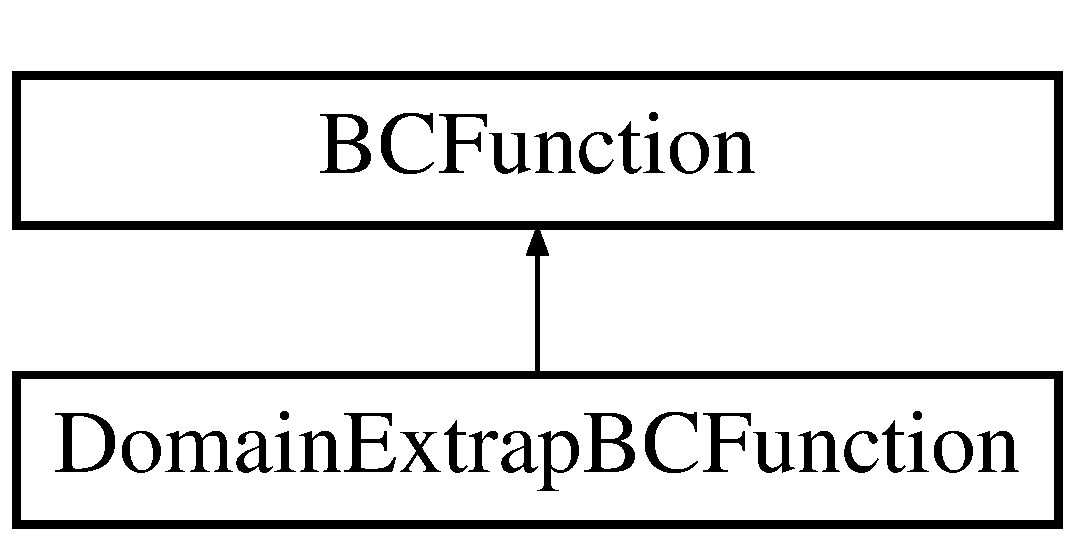
\includegraphics[height=2.000000cm]{class_domain_extrap_b_c_function}
\end{center}
\end{figure}
\subsection*{Public Member Functions}
\begin{DoxyCompactItemize}
\item 
\hypertarget{class_domain_extrap_b_c_function_a55a5528b06fed1fb88b785cf7d87fecc}{\hyperlink{class_domain_extrap_b_c_function_a55a5528b06fed1fb88b785cf7d87fecc}{Domain\-Extrap\-B\-C\-Function} ()}\label{class_domain_extrap_b_c_function_a55a5528b06fed1fb88b785cf7d87fecc}

\begin{DoxyCompactList}\small\item\em Default constructor. \end{DoxyCompactList}\item 
\hypertarget{class_domain_extrap_b_c_function_ad083a3d037a1a95e4f9dbcca09510379}{\hyperlink{class_domain_extrap_b_c_function_ad083a3d037a1a95e4f9dbcca09510379}{Domain\-Extrap\-B\-C\-Function} (bool a\-\_\-is\-Defined, \hyperlink{class_mushy_layer_params}{Mushy\-Layer\-Params} a\-\_\-params)}\label{class_domain_extrap_b_c_function_ad083a3d037a1a95e4f9dbcca09510379}

\begin{DoxyCompactList}\small\item\em Full constructor. \end{DoxyCompactList}\item 
\hypertarget{class_domain_extrap_b_c_function_a0131a3747f9d742a4c802aa460805f5f}{virtual void \hyperlink{class_domain_extrap_b_c_function_a0131a3747f9d742a4c802aa460805f5f}{operator()} (F\-Array\-Box \&a\-\_\-state, const Box \&a\-\_\-valid, const Problem\-Domain \&a\-\_\-domain, Real a\-\_\-dx, bool a\-\_\-homogeneous)}\label{class_domain_extrap_b_c_function_a0131a3747f9d742a4c802aa460805f5f}

\begin{DoxyCompactList}\small\item\em Apply B\-C. \end{DoxyCompactList}\end{DoxyCompactItemize}
\subsection*{Public Attributes}
\begin{DoxyCompactItemize}
\item 
\hypertarget{class_domain_extrap_b_c_function_adc313727aea12d585c4cda5752084a8a}{bool \hyperlink{class_domain_extrap_b_c_function_adc313727aea12d585c4cda5752084a8a}{m\-\_\-is\-Defined}}\label{class_domain_extrap_b_c_function_adc313727aea12d585c4cda5752084a8a}

\begin{DoxyCompactList}\small\item\em Is object defined? \end{DoxyCompactList}\item 
\hypertarget{class_domain_extrap_b_c_function_af988a9999fb0afb7f286c11ae85dc35c}{\hyperlink{class_mushy_layer_params}{Mushy\-Layer\-Params} \hyperlink{class_domain_extrap_b_c_function_af988a9999fb0afb7f286c11ae85dc35c}{m\-\_\-params}}\label{class_domain_extrap_b_c_function_af988a9999fb0afb7f286c11ae85dc35c}

\begin{DoxyCompactList}\small\item\em Physical parameters for the problem. \end{DoxyCompactList}\end{DoxyCompactItemize}


\subsection{Detailed Description}
Extrap Boundary condition. 

Extrapolation on all sides 

The documentation for this class was generated from the following file\-:\begin{DoxyCompactItemize}
\item 
/home/parkinsonjl/mushy-\/layer/\-B\-Cutil/Phys\-B\-C\-Util.\-cpp\end{DoxyCompactItemize}

\hypertarget{class_edge_vel_b_c_holder}{\section{Edge\-Vel\-B\-C\-Holder Class Reference}
\label{class_edge_vel_b_c_holder}\index{Edge\-Vel\-B\-C\-Holder@{Edge\-Vel\-B\-C\-Holder}}
}


this is a physical B\-C class designed to handle velocities on edges  




{\ttfamily \#include $<$Vel\-B\-C\-Holder.\-H$>$}

\subsection*{Public Member Functions}
\begin{DoxyCompactItemize}
\item 
\hypertarget{class_edge_vel_b_c_holder_aa2b8fa8269461af0855bfb1730868b15}{\hyperlink{class_edge_vel_b_c_holder_aa2b8fa8269461af0855bfb1730868b15}{Edge\-Vel\-B\-C\-Holder} ()}\label{class_edge_vel_b_c_holder_aa2b8fa8269461af0855bfb1730868b15}

\begin{DoxyCompactList}\small\item\em Default constructor. \end{DoxyCompactList}\item 
\hypertarget{class_edge_vel_b_c_holder_acf8f3b7abd18f5d2ebbeb652fc9350ee}{\hyperlink{class_edge_vel_b_c_holder_acf8f3b7abd18f5d2ebbeb652fc9350ee}{Edge\-Vel\-B\-C\-Holder} (const Tuple$<$ B\-C\-Holder, Space\-Dim $>$ \&a\-\_\-component\-B\-C)}\label{class_edge_vel_b_c_holder_acf8f3b7abd18f5d2ebbeb652fc9350ee}

\begin{DoxyCompactList}\small\item\em Full constructore. \end{DoxyCompactList}\item 
\hypertarget{class_edge_vel_b_c_holder_aa39ae49946806857b8136aea31e3f4ce}{virtual \hyperlink{class_edge_vel_b_c_holder_aa39ae49946806857b8136aea31e3f4ce}{$\sim$\-Edge\-Vel\-B\-C\-Holder} ()}\label{class_edge_vel_b_c_holder_aa39ae49946806857b8136aea31e3f4ce}

\begin{DoxyCompactList}\small\item\em Destructore. \end{DoxyCompactList}\item 
\hypertarget{class_edge_vel_b_c_holder_a9e4f58cb58cbefa89c76e8f2c5edc404}{virtual void \hyperlink{class_edge_vel_b_c_holder_a9e4f58cb58cbefa89c76e8f2c5edc404}{apply\-B\-Cs} (Level\-Data$<$ Flux\-Box $>$ \&a\-\_\-state, const Disjoint\-Box\-Layout \&a\-\_\-valid, const Problem\-Domain \&a\-\_\-domain, const Real a\-\_\-dx, bool a\-\_\-homogeneous)}\label{class_edge_vel_b_c_holder_a9e4f58cb58cbefa89c76e8f2c5edc404}

\begin{DoxyCompactList}\small\item\em Apply B\-Cs to a\-\_\-state. \end{DoxyCompactList}\end{DoxyCompactItemize}
\subsection*{Protected Attributes}
\begin{DoxyCompactItemize}
\item 
\hypertarget{class_edge_vel_b_c_holder_a80cc4520258374af4f7b76851d989bb2}{Tuple$<$ B\-C\-Holder, Space\-Dim $>$ \hyperlink{class_edge_vel_b_c_holder_a80cc4520258374af4f7b76851d989bb2}{m\-\_\-component\-B\-C}}\label{class_edge_vel_b_c_holder_a80cc4520258374af4f7b76851d989bb2}

\begin{DoxyCompactList}\small\item\em B\-C\-Holders for each component. \end{DoxyCompactList}\end{DoxyCompactItemize}


\subsection{Detailed Description}
this is a physical B\-C class designed to handle velocities on edges 

this class is handles velocities, which are by their nature multicomponent 

The documentation for this class was generated from the following files\-:\begin{DoxyCompactItemize}
\item 
/home/parkinsonjl/mushy-\/layer/\-B\-Cutil/Vel\-B\-C\-Holder.\-H\item 
/home/parkinsonjl/mushy-\/layer/\-B\-Cutil/Vel\-B\-C\-Holder.\-cpp\end{DoxyCompactItemize}

\hypertarget{class_extrapolation_b_c_function}{\section{Extrapolation\-B\-C\-Function Class Reference}
\label{class_extrapolation_b_c_function}\index{Extrapolation\-B\-C\-Function@{Extrapolation\-B\-C\-Function}}
}


Boundary condition for source terms.  


Inheritance diagram for Extrapolation\-B\-C\-Function\-:\begin{figure}[H]
\begin{center}
\leavevmode
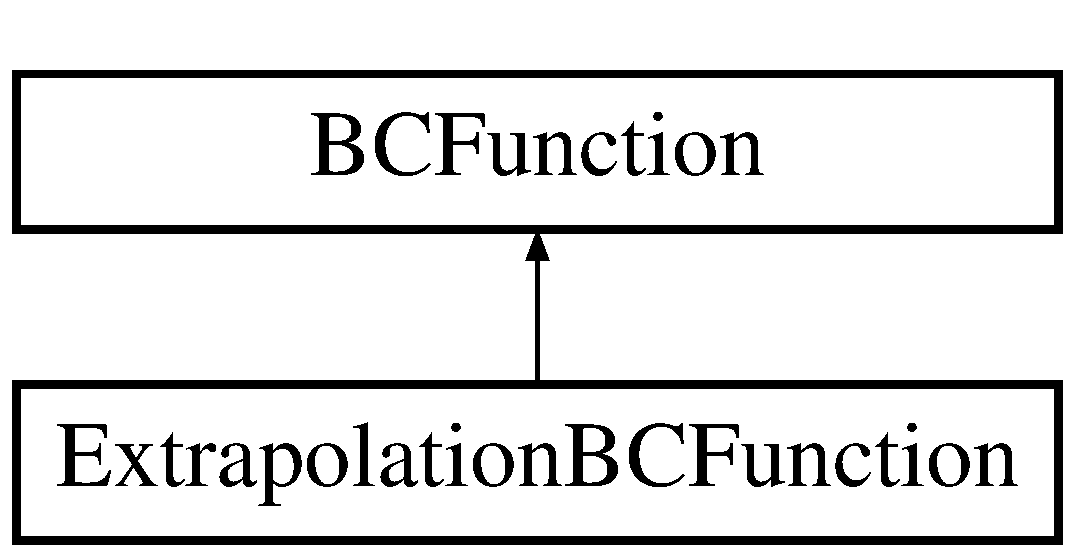
\includegraphics[height=2.000000cm]{class_extrapolation_b_c_function}
\end{center}
\end{figure}
\subsection*{Public Member Functions}
\begin{DoxyCompactItemize}
\item 
\hypertarget{class_extrapolation_b_c_function_ab6747f91f0d3ee6d32634cae85f62dd8}{\hyperlink{class_extrapolation_b_c_function_ab6747f91f0d3ee6d32634cae85f62dd8}{Extrapolation\-B\-C\-Function} (bool a\-\_\-is\-Defined, int a\-\_\-order=0)}\label{class_extrapolation_b_c_function_ab6747f91f0d3ee6d32634cae85f62dd8}

\begin{DoxyCompactList}\small\item\em Full constructor. \end{DoxyCompactList}\item 
\hypertarget{class_extrapolation_b_c_function_a3d8d0ed4cda1a8beb61c5ac5817b36aa}{virtual void \hyperlink{class_extrapolation_b_c_function_a3d8d0ed4cda1a8beb61c5ac5817b36aa}{operator()} (F\-Array\-Box \&a\-\_\-state, const Box \&a\-\_\-valid, const Problem\-Domain \&a\-\_\-domain, Real a\-\_\-dx, bool a\-\_\-homogeneous)}\label{class_extrapolation_b_c_function_a3d8d0ed4cda1a8beb61c5ac5817b36aa}

\begin{DoxyCompactList}\small\item\em Apply B\-C. \end{DoxyCompactList}\end{DoxyCompactItemize}
\subsection*{Public Attributes}
\begin{DoxyCompactItemize}
\item 
\hypertarget{class_extrapolation_b_c_function_a64590e6d6c7e4182ab3c5c9079620af3}{bool \hyperlink{class_extrapolation_b_c_function_a64590e6d6c7e4182ab3c5c9079620af3}{m\-\_\-is\-Defined}}\label{class_extrapolation_b_c_function_a64590e6d6c7e4182ab3c5c9079620af3}

\begin{DoxyCompactList}\small\item\em Is object defined? \end{DoxyCompactList}\item 
\hypertarget{class_extrapolation_b_c_function_a9fda57684ad22edeee9fb5c3b98a1469}{int {\bfseries m\-\_\-order}}\label{class_extrapolation_b_c_function_a9fda57684ad22edeee9fb5c3b98a1469}

\end{DoxyCompactItemize}


\subsection{Detailed Description}
Boundary condition for source terms. 

sets boundary conditions on source terms. At the moment, this is just 0th order extrapolation from the interior, so it's real simple. Fills interior as well as domain ghost cells. 

The documentation for this class was generated from the following file\-:\begin{DoxyCompactItemize}
\item 
/home/parkinsonjl/mushy-\/layer/\-B\-Cutil/Phys\-B\-C\-Util.\-cpp\end{DoxyCompactItemize}

\hypertarget{class_freestream_corr_b_c_function}{\section{Freestream\-Corr\-B\-C\-Function Class Reference}
\label{class_freestream_corr_b_c_function}\index{Freestream\-Corr\-B\-C\-Function@{Freestream\-Corr\-B\-C\-Function}}
}


Boundary condition for the freestream correction.  


Inheritance diagram for Freestream\-Corr\-B\-C\-Function\-:\begin{figure}[H]
\begin{center}
\leavevmode
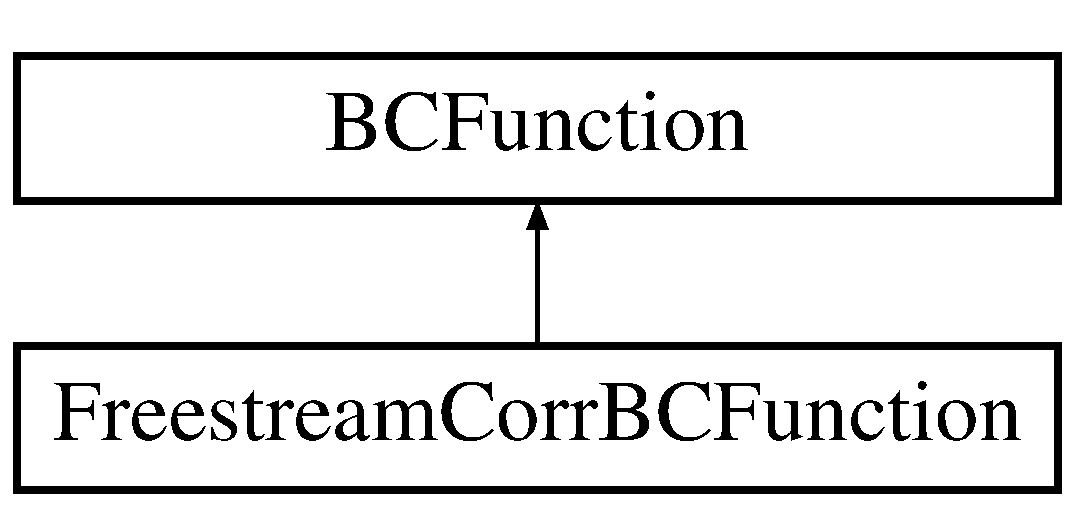
\includegraphics[height=2.000000cm]{class_freestream_corr_b_c_function}
\end{center}
\end{figure}
\subsection*{Public Member Functions}
\begin{DoxyCompactItemize}
\item 
\hypertarget{class_freestream_corr_b_c_function_a172724d0d72e728a531a314bdf487eff}{\hyperlink{class_freestream_corr_b_c_function_a172724d0d72e728a531a314bdf487eff}{Freestream\-Corr\-B\-C\-Function} ()}\label{class_freestream_corr_b_c_function_a172724d0d72e728a531a314bdf487eff}

\begin{DoxyCompactList}\small\item\em Default constructor. \end{DoxyCompactList}\item 
\hypertarget{class_freestream_corr_b_c_function_a6ef77a0c95d316d78af7a43d01f18fce}{\hyperlink{class_freestream_corr_b_c_function_a6ef77a0c95d316d78af7a43d01f18fce}{Freestream\-Corr\-B\-C\-Function} (bool a\-\_\-is\-Defined, \hyperlink{class_mushy_layer_params}{Mushy\-Layer\-Params} a\-\_\-params)}\label{class_freestream_corr_b_c_function_a6ef77a0c95d316d78af7a43d01f18fce}

\begin{DoxyCompactList}\small\item\em Full constructor. \end{DoxyCompactList}\item 
\hypertarget{class_freestream_corr_b_c_function_a3d1570440733a0cdc9eeb853774d0f60}{virtual void \hyperlink{class_freestream_corr_b_c_function_a3d1570440733a0cdc9eeb853774d0f60}{operator()} (F\-Array\-Box \&a\-\_\-state, const Box \&a\-\_\-valid, const Problem\-Domain \&a\-\_\-domain, Real a\-\_\-dx, bool a\-\_\-homogeneous)}\label{class_freestream_corr_b_c_function_a3d1570440733a0cdc9eeb853774d0f60}

\begin{DoxyCompactList}\small\item\em Apply B\-C. \end{DoxyCompactList}\end{DoxyCompactItemize}
\subsection*{Public Attributes}
\begin{DoxyCompactItemize}
\item 
\hypertarget{class_freestream_corr_b_c_function_ad6be36c1cc74d3b57f0e4e281facbb8b}{bool \hyperlink{class_freestream_corr_b_c_function_ad6be36c1cc74d3b57f0e4e281facbb8b}{m\-\_\-is\-Defined}}\label{class_freestream_corr_b_c_function_ad6be36c1cc74d3b57f0e4e281facbb8b}

\begin{DoxyCompactList}\small\item\em Is object defined? \end{DoxyCompactList}\item 
\hypertarget{class_freestream_corr_b_c_function_a263cee88a84aca937425bc75a14db918}{\hyperlink{class_mushy_layer_params}{Mushy\-Layer\-Params} \hyperlink{class_freestream_corr_b_c_function_a263cee88a84aca937425bc75a14db918}{m\-\_\-params}}\label{class_freestream_corr_b_c_function_a263cee88a84aca937425bc75a14db918}

\begin{DoxyCompactList}\small\item\em Physical parameters for the problem. \end{DoxyCompactList}\end{DoxyCompactItemize}


\subsection{Detailed Description}
Boundary condition for the freestream correction. 

sets normal gradient to be 0 

The documentation for this class was generated from the following file\-:\begin{DoxyCompactItemize}
\item 
/home/parkinsonjl/mushy-\/layer/\-B\-Cutil/Phys\-B\-C\-Util.\-cpp\end{DoxyCompactItemize}

\hypertarget{class_gradient}{\section{Gradient Class Reference}
\label{class_gradient}\index{Gradient@{Gradient}}
}


Class to encapsulate \hyperlink{class_gradient}{Gradient} functions (both C\-C and face-\/centered)  




{\ttfamily \#include $<$Gradient.\-H$>$}

\subsection*{Static Public Member Functions}
\begin{DoxyCompactItemize}
\item 
static void \hyperlink{class_gradient_aa657ff462b1dd44565ab4e5c35c097fa}{level\-Gradient\-C\-C} (Level\-Data$<$ F\-Array\-Box $>$ \&a\-\_\-grad, Level\-Data$<$ F\-Array\-Box $>$ \&a\-\_\-phi, const Level\-Data$<$ F\-Array\-Box $>$ $\ast$a\-\_\-phi\-Crse\-Ptr, const Real a\-\_\-dx, const int a\-\_\-n\-Ref\-Crse, const Problem\-Domain \&a\-\_\-d\-Problem)
\begin{DoxyCompactList}\small\item\em computes cell-\/centered level-\/operator gradient of cell-\/centered phi \end{DoxyCompactList}\item 
static void \hyperlink{class_gradient_a9e85cf629d0e4b0ad7809c0db1f0322c}{level\-Gradient\-C\-C} (Level\-Data$<$ F\-Array\-Box $>$ \&a\-\_\-grad, Level\-Data$<$ F\-Array\-Box $>$ \&a\-\_\-phi, const Level\-Data$<$ F\-Array\-Box $>$ $\ast$a\-\_\-phi\-Crse\-Ptr, const Real a\-\_\-dx, const int a\-\_\-n\-Ref\-Crse, const Box \&a\-\_\-d\-Problem)
\begin{DoxyCompactList}\small\item\em computes cell-\/centered level-\/operator gradient of cell-\/centered phi \end{DoxyCompactList}\item 
static void \hyperlink{class_gradient_a6a14b8f09f7882545497dcccac01e35e}{level\-Gradient\-C\-C} (Level\-Data$<$ F\-Array\-Box $>$ \&a\-\_\-grad, Level\-Data$<$ F\-Array\-Box $>$ \&a\-\_\-phi, const Level\-Data$<$ F\-Array\-Box $>$ $\ast$a\-\_\-phi\-Crse\-Ptr, const Real a\-\_\-dx, const Layout\-Data$<$ Int\-Vect\-Set $>$ \&a\-\_\-grid\-I\-V\-S, Quad\-C\-F\-Interp \&a\-\_\-cf\-Interp)
\begin{DoxyCompactList}\small\item\em computes cell-\/centered level-\/operator gradient of cell-\/centered phi \end{DoxyCompactList}\item 
static void \hyperlink{class_gradient_a6103f7090b4d658cc1086f31a47474ba}{level\-Gradient\-C\-C} (Level\-Data$<$ F\-Array\-Box $>$ \&a\-\_\-grad, const Level\-Data$<$ F\-Array\-Box $>$ \&a\-\_\-phi, const Real a\-\_\-dx)
\begin{DoxyCompactList}\small\item\em computes cell-\/centered, level-\/operator gradient of cell-\/centered phi \end{DoxyCompactList}\item 
static void \hyperlink{class_gradient_a8962d5f7dabe25690dce34ce1c00726d}{level\-Gradient\-C\-C} (Level\-Data$<$ F\-Array\-Box $>$ \&a\-\_\-grad, const Level\-Data$<$ Flux\-Box $>$ \&a\-\_\-phi, const Real a\-\_\-dx)
\begin{DoxyCompactList}\small\item\em computes cell-\/centered, level-\/operator gradient of face-\/centered phi \end{DoxyCompactList}\item 
static void \hyperlink{class_gradient_a476a6adb3c37375c48b60d91a3c9c949}{level\-Gradient\-C\-C} (Level\-Data$<$ F\-Array\-Box $>$ \&a\-\_\-grad, const Level\-Data$<$ F\-Array\-Box $>$ \&a\-\_\-phi, const Real a\-\_\-dx, const int n\-Ghost)
\begin{DoxyCompactList}\small\item\em computes cell-\/centered, level-\/operator gradient of cell-\/centered phi \end{DoxyCompactList}\item 
static void \hyperlink{class_gradient_ab5fa9029705d216a3c1ae97b58bb970e}{level\-Gradient\-C\-C\-Upwind} (Level\-Data$<$ F\-Array\-Box $>$ \&a\-\_\-grad, const Level\-Data$<$ F\-Array\-Box $>$ \&a\-\_\-phi, const Real a\-\_\-dx)
\begin{DoxyCompactList}\small\item\em computes onesided, level-\/operator gradient of cell-\/centered phi \end{DoxyCompactList}\item 
static void \hyperlink{class_gradient_ab55b4c85431294e40707bd0bdae6e012}{level\-Gradient\-C\-C\-Upwind} (Level\-Data$<$ F\-Array\-Box $>$ \&a\-\_\-grad, const Level\-Data$<$ F\-Array\-Box $>$ \&a\-\_\-phi, const Real a\-\_\-dx, const Side\-::\-Lo\-Hi\-Side extrap\-Side, int order=2)
\begin{DoxyCompactList}\small\item\em computes level-\/operator gradient of cell-\/centred phi \end{DoxyCompactList}\item 
static void \hyperlink{class_gradient_a00daa2aa0e66c5f70545cbd9cdf633a2}{level\-Gradient\-C\-C\-New\-One\-Sided} (Level\-Data$<$ F\-Array\-Box $>$ \&a\-\_\-grad, const Level\-Data$<$ F\-Array\-Box $>$ \&a\-\_\-phi, const Real a\-\_\-dx, int order=2)
\begin{DoxyCompactList}\small\item\em computes level-\/operator gradient of cell-\/centered phi \end{DoxyCompactList}\item 
static void \hyperlink{class_gradient_a306b5f347d51c38d5cf8a7f446ea0b86}{level\-Gradient\-C\-C\-New\-Centred} (Level\-Data$<$ F\-Array\-Box $>$ \&a\-\_\-grad, const Level\-Data$<$ F\-Array\-Box $>$ \&a\-\_\-phi, const Real a\-\_\-dx, int order=2)
\item 
static void \hyperlink{class_gradient_a6c741fa4909be6c7d55ddc70a128ca93}{comp\-Gradient\-C\-C} (Level\-Data$<$ F\-Array\-Box $>$ \&a\-\_\-grad, Level\-Data$<$ F\-Array\-Box $>$ \&a\-\_\-phi, const Level\-Data$<$ F\-Array\-Box $>$ $\ast$a\-\_\-phi\-Crse\-Ptr, const Level\-Data$<$ F\-Array\-Box $>$ $\ast$a\-\_\-phi\-Fine\-Ptr, const Real a\-\_\-dx, const int a\-\_\-n\-Ref\-Crse, const int a\-\_\-n\-Ref\-Fine, const Problem\-Domain \&a\-\_\-d\-Problem)
\begin{DoxyCompactList}\small\item\em computes cell-\/centered composite gradient of cell centered phi \end{DoxyCompactList}\item 
static void \hyperlink{class_gradient_a0a941dcb9ad58ed819f41d4fe1080106}{comp\-Gradient\-C\-C} (Level\-Data$<$ F\-Array\-Box $>$ \&a\-\_\-grad, Level\-Data$<$ F\-Array\-Box $>$ \&a\-\_\-phi, const Level\-Data$<$ F\-Array\-Box $>$ $\ast$a\-\_\-phi\-Crse\-Ptr, const Level\-Data$<$ F\-Array\-Box $>$ $\ast$a\-\_\-phi\-Fine\-Ptr, const Real a\-\_\-dx, const int a\-\_\-n\-Ref\-Crse, const int a\-\_\-n\-Ref\-Fine, const Box \&a\-\_\-d\-Problem)
\begin{DoxyCompactList}\small\item\em computes cell-\/centered composite gradient of cell centered phi \end{DoxyCompactList}\item 
static void \hyperlink{class_gradient_a029f7d1cb39888c2e12b9fb016b58928}{comp\-Gradient\-C\-C} (Level\-Data$<$ F\-Array\-Box $>$ \&a\-\_\-grad, Level\-Data$<$ F\-Array\-Box $>$ \&a\-\_\-phi, const Level\-Data$<$ F\-Array\-Box $>$ $\ast$a\-\_\-phi\-Crse\-Ptr, const Level\-Data$<$ F\-Array\-Box $>$ $\ast$a\-\_\-phi\-Fine\-Ptr, const Real a\-\_\-dx, const int a\-\_\-n\-Ref\-Fine, const Problem\-Domain \&a\-\_\-d\-Problem, const Layout\-Data$<$ Int\-Vect\-Set $>$ \&a\-\_\-grid\-I\-V\-S, Quad\-C\-F\-Interp \&a\-\_\-cf\-Interp\-Crse)
\begin{DoxyCompactList}\small\item\em computes cell-\/centered composite gradient of cell-\/centered phi \end{DoxyCompactList}\item 
static void \hyperlink{class_gradient_a4f44d7eef3d2b675d9c67c90b9904747}{comp\-Gradient\-C\-C} (Level\-Data$<$ F\-Array\-Box $>$ \&a\-\_\-grad, Level\-Data$<$ F\-Array\-Box $>$ \&a\-\_\-phi, const Level\-Data$<$ F\-Array\-Box $>$ $\ast$a\-\_\-phi\-Crse\-Ptr, const Level\-Data$<$ F\-Array\-Box $>$ $\ast$a\-\_\-phi\-Fine\-Ptr, const Real a\-\_\-dx, const int a\-\_\-n\-Ref\-Fine, const Box \&a\-\_\-d\-Problem, const Layout\-Data$<$ Int\-Vect\-Set $>$ \&a\-\_\-grid\-I\-V\-S, Quad\-C\-F\-Interp \&a\-\_\-cf\-Interp\-Crse)
\begin{DoxyCompactList}\small\item\em computes cell-\/centered composite gradient of cell-\/centered phi \end{DoxyCompactList}\item 
static void \hyperlink{class_gradient_a23967a97f57bc4c1609e63faa2eaf437}{comp\-Gradient\-C\-C} (Level\-Data$<$ F\-Array\-Box $>$ \&a\-\_\-\-Grad, const Level\-Data$<$ F\-Array\-Box $>$ \&a\-\_\-phi, const Level\-Data$<$ F\-Array\-Box $>$ $\ast$a\-\_\-phi\-Fine\-Ptr, const Real a\-\_\-dx, const int a\-\_\-n\-Ref\-Fine, const Problem\-Domain \&a\-\_\-d\-Problem)
\begin{DoxyCompactList}\small\item\em computes cell-\/centered composite gradient of cell-\/centered phi \end{DoxyCompactList}\item 
static void \hyperlink{class_gradient_ad59fcf73da0f075761f2363b1d1e6c2b}{comp\-Gradient\-C\-C} (Level\-Data$<$ F\-Array\-Box $>$ \&a\-\_\-\-Grad, const Level\-Data$<$ F\-Array\-Box $>$ \&a\-\_\-phi, const Level\-Data$<$ F\-Array\-Box $>$ $\ast$a\-\_\-phi\-Fine\-Ptr, const Real a\-\_\-dx, const int a\-\_\-n\-Ref\-Fine, const Box \&a\-\_\-d\-Problem)
\begin{DoxyCompactList}\small\item\em computes cell-\/centered composite gradient of cell-\/centered phi \end{DoxyCompactList}\item 
static void \hyperlink{class_gradient_a7d6a189f7e14c864e35ef507128c9113}{level\-Gradient\-M\-A\-C} (Level\-Data$<$ Flux\-Box $>$ \&a\-\_\-edge\-Grad, Level\-Data$<$ F\-Array\-Box $>$ \&a\-\_\-phi, const Level\-Data$<$ F\-Array\-Box $>$ $\ast$a\-\_\-phi\-Crse\-Ptr, const Real a\-\_\-dx, const int a\-\_\-n\-Ref\-Crse, const Problem\-Domain \&a\-\_\-d\-Problem)
\begin{DoxyCompactList}\small\item\em computes edge-\/centered level-\/operator gradient of cell-\/centered phi \end{DoxyCompactList}\item 
static void \hyperlink{class_gradient_a984db420418480a063fa7e60dc18144d}{level\-Gradient\-M\-A\-C} (Level\-Data$<$ Flux\-Box $>$ \&a\-\_\-edge\-Grad, Level\-Data$<$ F\-Array\-Box $>$ \&a\-\_\-phi, const Level\-Data$<$ F\-Array\-Box $>$ $\ast$a\-\_\-phi\-Crse\-Ptr, const Real a\-\_\-dx, const int a\-\_\-n\-Ref\-Crse, const Box \&a\-\_\-d\-Problem)
\begin{DoxyCompactList}\small\item\em computes edge-\/centered level-\/operator gradient of cell-\/centered phi \end{DoxyCompactList}\item 
static void \hyperlink{class_gradient_a1e5777612a7ff994896d694e2c1c816b}{level\-Gradient\-M\-A\-C} (Level\-Data$<$ Flux\-Box $>$ \&a\-\_\-edge\-Grad, Level\-Data$<$ F\-Array\-Box $>$ \&a\-\_\-phi, const Level\-Data$<$ F\-Array\-Box $>$ $\ast$a\-\_\-phi\-Crse\-Ptr, const Real a\-\_\-dx, const Layout\-Data$<$ Int\-Vect\-Set $>$ \&a\-\_\-grid\-I\-V\-S, Quad\-C\-F\-Interp \&a\-\_\-cf\-Interp\-Crse)
\begin{DoxyCompactList}\small\item\em computes edge-\/centered level-\/operator gradient of cell-\/centered phi \end{DoxyCompactList}\item 
static void \hyperlink{class_gradient_a3d95193c15462219bd5159de5341b291}{level\-Gradient\-M\-A\-C} (Level\-Data$<$ Flux\-Box $>$ \&a\-\_\-edge\-Grad, const Level\-Data$<$ F\-Array\-Box $>$ \&a\-\_\-phi, const Real a\-\_\-dx)
\begin{DoxyCompactList}\small\item\em computes edge-\/centered level-\/operator gradient of cell-\/centered phi \end{DoxyCompactList}\item 
\hypertarget{class_gradient_a9346502d05a030c51820bc034816d898}{static void \hyperlink{class_gradient_a9346502d05a030c51820bc034816d898}{level\-Gradient\-M\-A\-C\-New} (Level\-Data$<$ Flux\-Box $>$ \&a\-\_\-edge\-Grad, const Level\-Data$<$ F\-Array\-Box $>$ \&a\-\_\-phi, const Real a\-\_\-dx)}\label{class_gradient_a9346502d05a030c51820bc034816d898}

\begin{DoxyCompactList}\small\item\em Edge centred gradient, new version, assume ghost cells have been set. \end{DoxyCompactList}\item 
static void \hyperlink{class_gradient_a50d364c2e9951e70a74200537ebbd73d}{comp\-Gradient\-M\-A\-C} (Level\-Data$<$ Flux\-Box $>$ \&a\-\_\-edge\-Grad, Level\-Data$<$ F\-Array\-Box $>$ \&a\-\_\-phi, const Level\-Data$<$ F\-Array\-Box $>$ $\ast$a\-\_\-phi\-Crse, const Level\-Data$<$ F\-Array\-Box $>$ $\ast$a\-\_\-phi\-Fine, const Real a\-\_\-dx, const int a\-\_\-n\-Ref\-Crse, const int a\-\_\-n\-Ref\-Fine, const Box \&a\-\_\-d\-Problem)
\begin{DoxyCompactList}\small\item\em computes edge-\/centered composite gradient of cell-\/centered phi \end{DoxyCompactList}\item 
static void \hyperlink{class_gradient_ab53c80ecc42d684acd3456c47b4db5f2}{comp\-Gradient\-M\-A\-C} (Level\-Data$<$ Flux\-Box $>$ \&a\-\_\-edge\-Grad, Level\-Data$<$ F\-Array\-Box $>$ \&a\-\_\-phi, const Level\-Data$<$ F\-Array\-Box $>$ $\ast$a\-\_\-phi\-Crse, const Level\-Data$<$ F\-Array\-Box $>$ $\ast$a\-\_\-phi\-Fine, const Real a\-\_\-dx, const int a\-\_\-n\-Ref\-Crse, const int a\-\_\-n\-Ref\-Fine, const Problem\-Domain \&a\-\_\-d\-Problem)
\begin{DoxyCompactList}\small\item\em computes edge-\/centered composite gradient of cell-\/centered phi \end{DoxyCompactList}\item 
static void \hyperlink{class_gradient_a82e5e91499de8d5cbddf3c42528c9421}{comp\-Gradient\-M\-A\-C} (Level\-Data$<$ Flux\-Box $>$ \&a\-\_\-edge\-Grad, Level\-Data$<$ F\-Array\-Box $>$ \&a\-\_\-phi, const Level\-Data$<$ F\-Array\-Box $>$ $\ast$a\-\_\-phi\-Crse, const Level\-Data$<$ F\-Array\-Box $>$ $\ast$a\-\_\-phi\-Fine, const Real a\-\_\-dx, const int a\-\_\-n\-Ref\-Fine, const Layout\-Data$<$ Int\-Vect\-Set $>$ \&a\-\_\-grid\-I\-V\-S, Quad\-C\-F\-Interp \&a\-\_\-cf\-Interp\-Crse)
\begin{DoxyCompactList}\small\item\em computes edge-\/centered composite gradient of cell-\/centered phi \end{DoxyCompactList}\item 
\hypertarget{class_gradient_a54d7c331f9bf1ee1b95f6683b5ef4ca3}{static void \hyperlink{class_gradient_a54d7c331f9bf1ee1b95f6683b5ef4ca3}{single\-Box\-Mac\-Grad} (F\-Array\-Box \&a\-\_\-grad\-Fab, const F\-Array\-Box \&a\-\_\-phi\-Fab, int a\-\_\-grad\-Comp, int a\-\_\-phi\-Comp, int a\-\_\-num\-Comp, const Box \&a\-\_\-edge\-Box, Real a\-\_\-dx, int a\-\_\-dir, int a\-\_\-edge\-Dir, const Int\-Vect\-Set \&a\-\_\-grid\-I\-V\-S)}\label{class_gradient_a54d7c331f9bf1ee1b95f6683b5ef4ca3}

\begin{DoxyCompactList}\small\item\em utility function for internal use \end{DoxyCompactList}\item 
static void \hyperlink{class_gradient_a85f5cea4187536e8430d485a306b131d}{create\-Grid\-I\-V\-S} (Layout\-Data$<$ Int\-Vect\-Set $>$ \&a\-\_\-grids\-I\-V\-S, const Disjoint\-Box\-Layout \&a\-\_\-grids, const int a\-\_\-n\-Grow)
\begin{DoxyCompactList}\small\item\em create grid I\-V\-S for all grids \end{DoxyCompactList}\item 
static void \hyperlink{class_gradient_ab8d450f2f5e455e2a33ef3a33b2f5a98}{create\-Grid\-I\-V\-S} (Int\-Vect\-Set \&a\-\_\-grid\-I\-V\-S, const Disjoint\-Box\-Layout \&a\-\_\-grids, const Box \&a\-\_\-local\-Box, const int a\-\_\-n\-Grow=1)
\begin{DoxyCompactList}\small\item\em internal utility function \end{DoxyCompactList}\end{DoxyCompactItemize}


\subsection{Detailed Description}
Class to encapsulate \hyperlink{class_gradient}{Gradient} functions (both C\-C and face-\/centered) 

\subsection{Member Function Documentation}
\hypertarget{class_gradient_a6c741fa4909be6c7d55ddc70a128ca93}{\index{Gradient@{Gradient}!comp\-Gradient\-C\-C@{comp\-Gradient\-C\-C}}
\index{comp\-Gradient\-C\-C@{comp\-Gradient\-C\-C}!Gradient@{Gradient}}
\subsubsection[{comp\-Gradient\-C\-C}]{\setlength{\rightskip}{0pt plus 5cm}void Gradient\-::comp\-Gradient\-C\-C (
\begin{DoxyParamCaption}
\item[{Level\-Data$<$ F\-Array\-Box $>$ \&}]{a\-\_\-grad, }
\item[{Level\-Data$<$ F\-Array\-Box $>$ \&}]{a\-\_\-phi, }
\item[{const Level\-Data$<$ F\-Array\-Box $>$ $\ast$}]{a\-\_\-phi\-Crse\-Ptr, }
\item[{const Level\-Data$<$ F\-Array\-Box $>$ $\ast$}]{a\-\_\-phi\-Fine\-Ptr, }
\item[{const Real}]{a\-\_\-dx, }
\item[{const int}]{a\-\_\-n\-Ref\-Crse, }
\item[{const int}]{a\-\_\-n\-Ref\-Fine, }
\item[{const Problem\-Domain \&}]{a\-\_\-d\-Problem}
\end{DoxyParamCaption}
)\hspace{0.3cm}{\ttfamily [static]}}}\label{class_gradient_a6c741fa4909be6c7d55ddc70a128ca93}


computes cell-\/centered composite gradient of cell centered phi 

Uses same coarse-\/level C/\-F B\-C's as Level\-Gradient\-C\-C, if phi\-Fine\-Ptr != N\-U\-L\-L, then also uses one-\/sided differencing to compute gradient on coarse side of coarse-\/fine interface. \hypertarget{class_gradient_a0a941dcb9ad58ed819f41d4fe1080106}{\index{Gradient@{Gradient}!comp\-Gradient\-C\-C@{comp\-Gradient\-C\-C}}
\index{comp\-Gradient\-C\-C@{comp\-Gradient\-C\-C}!Gradient@{Gradient}}
\subsubsection[{comp\-Gradient\-C\-C}]{\setlength{\rightskip}{0pt plus 5cm}void Gradient\-::comp\-Gradient\-C\-C (
\begin{DoxyParamCaption}
\item[{Level\-Data$<$ F\-Array\-Box $>$ \&}]{a\-\_\-grad, }
\item[{Level\-Data$<$ F\-Array\-Box $>$ \&}]{a\-\_\-phi, }
\item[{const Level\-Data$<$ F\-Array\-Box $>$ $\ast$}]{a\-\_\-phi\-Crse\-Ptr, }
\item[{const Level\-Data$<$ F\-Array\-Box $>$ $\ast$}]{a\-\_\-phi\-Fine\-Ptr, }
\item[{const Real}]{a\-\_\-dx, }
\item[{const int}]{a\-\_\-n\-Ref\-Crse, }
\item[{const int}]{a\-\_\-n\-Ref\-Fine, }
\item[{const Box \&}]{a\-\_\-d\-Problem}
\end{DoxyParamCaption}
)\hspace{0.3cm}{\ttfamily [static]}}}\label{class_gradient_a0a941dcb9ad58ed819f41d4fe1080106}


computes cell-\/centered composite gradient of cell centered phi 

uses same coarse-\/level C/\-F B\-C's as Level\-Gradient\-C\-C, if phi\-Fine\-Ptr != N\-U\-L\-L, then also uses one-\/sided differencing to compute gradient on coarse side of coarse-\/fine interface. This (deprecated) interface uses a Box instead of a Problem\-Domain \hypertarget{class_gradient_a029f7d1cb39888c2e12b9fb016b58928}{\index{Gradient@{Gradient}!comp\-Gradient\-C\-C@{comp\-Gradient\-C\-C}}
\index{comp\-Gradient\-C\-C@{comp\-Gradient\-C\-C}!Gradient@{Gradient}}
\subsubsection[{comp\-Gradient\-C\-C}]{\setlength{\rightskip}{0pt plus 5cm}void Gradient\-::comp\-Gradient\-C\-C (
\begin{DoxyParamCaption}
\item[{Level\-Data$<$ F\-Array\-Box $>$ \&}]{a\-\_\-grad, }
\item[{Level\-Data$<$ F\-Array\-Box $>$ \&}]{a\-\_\-phi, }
\item[{const Level\-Data$<$ F\-Array\-Box $>$ $\ast$}]{a\-\_\-phi\-Crse\-Ptr, }
\item[{const Level\-Data$<$ F\-Array\-Box $>$ $\ast$}]{a\-\_\-phi\-Fine\-Ptr, }
\item[{const Real}]{a\-\_\-dx, }
\item[{const int}]{a\-\_\-n\-Ref\-Fine, }
\item[{const Problem\-Domain \&}]{a\-\_\-d\-Problem, }
\item[{const Layout\-Data$<$ Int\-Vect\-Set $>$ \&}]{a\-\_\-grid\-I\-V\-S, }
\item[{Quad\-C\-F\-Interp \&}]{a\-\_\-cf\-Interp\-Crse}
\end{DoxyParamCaption}
)\hspace{0.3cm}{\ttfamily [static]}}}\label{class_gradient_a029f7d1cb39888c2e12b9fb016b58928}


computes cell-\/centered composite gradient of cell-\/centered phi 

uses same coarse-\/level C/\-F B\-C's as Level\-Gradient\-C\-C, if phi\-Fine\-Ptr != N\-U\-L\-L, then also uses one-\/sided differencing to compute gradient on coarse side of coarse-\/fine interface. A predefined Quad\-C\-F\-Interp is also passed in for efficiency. Note that no fine Quad\-C\-F\-Interp is necessary because we use one-\/sided differencing for coarse cells adjacent to finer-\/level coarse-\/fine interfaces. Note also that gradient is only really defined in valid regions of grids. \hypertarget{class_gradient_a4f44d7eef3d2b675d9c67c90b9904747}{\index{Gradient@{Gradient}!comp\-Gradient\-C\-C@{comp\-Gradient\-C\-C}}
\index{comp\-Gradient\-C\-C@{comp\-Gradient\-C\-C}!Gradient@{Gradient}}
\subsubsection[{comp\-Gradient\-C\-C}]{\setlength{\rightskip}{0pt plus 5cm}void Gradient\-::comp\-Gradient\-C\-C (
\begin{DoxyParamCaption}
\item[{Level\-Data$<$ F\-Array\-Box $>$ \&}]{a\-\_\-grad, }
\item[{Level\-Data$<$ F\-Array\-Box $>$ \&}]{a\-\_\-phi, }
\item[{const Level\-Data$<$ F\-Array\-Box $>$ $\ast$}]{a\-\_\-phi\-Crse\-Ptr, }
\item[{const Level\-Data$<$ F\-Array\-Box $>$ $\ast$}]{a\-\_\-phi\-Fine\-Ptr, }
\item[{const Real}]{a\-\_\-dx, }
\item[{const int}]{a\-\_\-n\-Ref\-Fine, }
\item[{const Box \&}]{a\-\_\-d\-Problem, }
\item[{const Layout\-Data$<$ Int\-Vect\-Set $>$ \&}]{a\-\_\-grid\-I\-V\-S, }
\item[{Quad\-C\-F\-Interp \&}]{a\-\_\-cf\-Interp\-Crse}
\end{DoxyParamCaption}
)\hspace{0.3cm}{\ttfamily [static]}}}\label{class_gradient_a4f44d7eef3d2b675d9c67c90b9904747}


computes cell-\/centered composite gradient of cell-\/centered phi 

uses same coarse-\/level C/\-F B\-C's as Level\-Gradient\-C\-C, if phi\-Fine\-Ptr != N\-U\-L\-L, then also uses one-\/sided differencing to compute gradient on coarse side of coarse-\/fine interface. A predefined Quad\-C\-F\-Interp is also passed in for efficiency. Note that no fine Quad\-C\-F\-Interp is necessary because we use one-\/sided differencing for coarse cells adjacent to finer-\/level coarse-\/fine interfaces. Note also that gradient is only really defined in valid regions of grids. This (deprecated) interface uses a Box instead of a Problem\-Domain \hypertarget{class_gradient_a23967a97f57bc4c1609e63faa2eaf437}{\index{Gradient@{Gradient}!comp\-Gradient\-C\-C@{comp\-Gradient\-C\-C}}
\index{comp\-Gradient\-C\-C@{comp\-Gradient\-C\-C}!Gradient@{Gradient}}
\subsubsection[{comp\-Gradient\-C\-C}]{\setlength{\rightskip}{0pt plus 5cm}void Gradient\-::comp\-Gradient\-C\-C (
\begin{DoxyParamCaption}
\item[{Level\-Data$<$ F\-Array\-Box $>$ \&}]{a\-\_\-\-Grad, }
\item[{const Level\-Data$<$ F\-Array\-Box $>$ \&}]{a\-\_\-phi, }
\item[{const Level\-Data$<$ F\-Array\-Box $>$ $\ast$}]{a\-\_\-phi\-Fine\-Ptr, }
\item[{const Real}]{a\-\_\-dx, }
\item[{const int}]{a\-\_\-n\-Ref\-Fine, }
\item[{const Problem\-Domain \&}]{a\-\_\-d\-Problem}
\end{DoxyParamCaption}
)\hspace{0.3cm}{\ttfamily [static]}}}\label{class_gradient_a23967a97f57bc4c1609e63faa2eaf437}


computes cell-\/centered composite gradient of cell-\/centered phi 

this one assumes that all ghost-\/cell values have already been set; if phi\-Fine\-Ptr != N\-U\-L\-L, then also uses one-\/sided differencing to compute gradient on coarse side of corarse-\/fine interface. note that gradient is only really defined in valid regions of grids. \hypertarget{class_gradient_ad59fcf73da0f075761f2363b1d1e6c2b}{\index{Gradient@{Gradient}!comp\-Gradient\-C\-C@{comp\-Gradient\-C\-C}}
\index{comp\-Gradient\-C\-C@{comp\-Gradient\-C\-C}!Gradient@{Gradient}}
\subsubsection[{comp\-Gradient\-C\-C}]{\setlength{\rightskip}{0pt plus 5cm}void Gradient\-::comp\-Gradient\-C\-C (
\begin{DoxyParamCaption}
\item[{Level\-Data$<$ F\-Array\-Box $>$ \&}]{a\-\_\-\-Grad, }
\item[{const Level\-Data$<$ F\-Array\-Box $>$ \&}]{a\-\_\-phi, }
\item[{const Level\-Data$<$ F\-Array\-Box $>$ $\ast$}]{a\-\_\-phi\-Fine\-Ptr, }
\item[{const Real}]{a\-\_\-dx, }
\item[{const int}]{a\-\_\-n\-Ref\-Fine, }
\item[{const Box \&}]{a\-\_\-d\-Problem}
\end{DoxyParamCaption}
)\hspace{0.3cm}{\ttfamily [static]}}}\label{class_gradient_ad59fcf73da0f075761f2363b1d1e6c2b}


computes cell-\/centered composite gradient of cell-\/centered phi 

this one assumes that all ghost-\/cell values have already been set; if phi\-Fine\-Ptr != N\-U\-L\-L, then also uses one-\/sided differencing to compute gradient on coarse side of corarse-\/fine interface. note that gradient is only really defined in valid regions of grids. This (deprecated) interface uses a Box instead of a Problem\-Domain \hypertarget{class_gradient_a50d364c2e9951e70a74200537ebbd73d}{\index{Gradient@{Gradient}!comp\-Gradient\-M\-A\-C@{comp\-Gradient\-M\-A\-C}}
\index{comp\-Gradient\-M\-A\-C@{comp\-Gradient\-M\-A\-C}!Gradient@{Gradient}}
\subsubsection[{comp\-Gradient\-M\-A\-C}]{\setlength{\rightskip}{0pt plus 5cm}void Gradient\-::comp\-Gradient\-M\-A\-C (
\begin{DoxyParamCaption}
\item[{Level\-Data$<$ Flux\-Box $>$ \&}]{a\-\_\-edge\-Grad, }
\item[{Level\-Data$<$ F\-Array\-Box $>$ \&}]{a\-\_\-phi, }
\item[{const Level\-Data$<$ F\-Array\-Box $>$ $\ast$}]{a\-\_\-phi\-Crse, }
\item[{const Level\-Data$<$ F\-Array\-Box $>$ $\ast$}]{a\-\_\-phi\-Fine, }
\item[{const Real}]{a\-\_\-dx, }
\item[{const int}]{a\-\_\-n\-Ref\-Crse, }
\item[{const int}]{a\-\_\-n\-Ref\-Fine, }
\item[{const Box \&}]{a\-\_\-d\-Problem}
\end{DoxyParamCaption}
)\hspace{0.3cm}{\ttfamily [static]}}}\label{class_gradient_a50d364c2e9951e70a74200537ebbd73d}


computes edge-\/centered composite gradient of cell-\/centered phi 

if phi\-Crse\-Ptr != N\-U\-L\-L, does quadratic interpolation to compute coarse-\/fine boundary conditions for phi; since the edge between this level and finer levels is not considered to be a part of this level, there is no fine-\/level coarse-\/fine B\-C. because of this, this function produces exactly the same results as Level\-Gradient\-M\-A\-C -- it's just included for completeness... \hypertarget{class_gradient_ab53c80ecc42d684acd3456c47b4db5f2}{\index{Gradient@{Gradient}!comp\-Gradient\-M\-A\-C@{comp\-Gradient\-M\-A\-C}}
\index{comp\-Gradient\-M\-A\-C@{comp\-Gradient\-M\-A\-C}!Gradient@{Gradient}}
\subsubsection[{comp\-Gradient\-M\-A\-C}]{\setlength{\rightskip}{0pt plus 5cm}void Gradient\-::comp\-Gradient\-M\-A\-C (
\begin{DoxyParamCaption}
\item[{Level\-Data$<$ Flux\-Box $>$ \&}]{a\-\_\-edge\-Grad, }
\item[{Level\-Data$<$ F\-Array\-Box $>$ \&}]{a\-\_\-phi, }
\item[{const Level\-Data$<$ F\-Array\-Box $>$ $\ast$}]{a\-\_\-phi\-Crse, }
\item[{const Level\-Data$<$ F\-Array\-Box $>$ $\ast$}]{a\-\_\-phi\-Fine, }
\item[{const Real}]{a\-\_\-dx, }
\item[{const int}]{a\-\_\-n\-Ref\-Crse, }
\item[{const int}]{a\-\_\-n\-Ref\-Fine, }
\item[{const Problem\-Domain \&}]{a\-\_\-d\-Problem}
\end{DoxyParamCaption}
)\hspace{0.3cm}{\ttfamily [static]}}}\label{class_gradient_ab53c80ecc42d684acd3456c47b4db5f2}


computes edge-\/centered composite gradient of cell-\/centered phi 

if phi\-Crse\-Ptr != N\-U\-L\-L, does quadratic interpolation to compute coarse-\/fine boundary conditions for phi; since the edge between this level and finer levels is not considered to be a part of this level, there is no fine-\/level coarse-\/fine B\-C. because of this, this function produces exactly the same results as Level\-Gradient\-M\-A\-C -- it's just included for completeness... \hypertarget{class_gradient_a82e5e91499de8d5cbddf3c42528c9421}{\index{Gradient@{Gradient}!comp\-Gradient\-M\-A\-C@{comp\-Gradient\-M\-A\-C}}
\index{comp\-Gradient\-M\-A\-C@{comp\-Gradient\-M\-A\-C}!Gradient@{Gradient}}
\subsubsection[{comp\-Gradient\-M\-A\-C}]{\setlength{\rightskip}{0pt plus 5cm}void Gradient\-::comp\-Gradient\-M\-A\-C (
\begin{DoxyParamCaption}
\item[{Level\-Data$<$ Flux\-Box $>$ \&}]{a\-\_\-edge\-Grad, }
\item[{Level\-Data$<$ F\-Array\-Box $>$ \&}]{a\-\_\-phi, }
\item[{const Level\-Data$<$ F\-Array\-Box $>$ $\ast$}]{a\-\_\-phi\-Crse, }
\item[{const Level\-Data$<$ F\-Array\-Box $>$ $\ast$}]{a\-\_\-phi\-Fine, }
\item[{const Real}]{a\-\_\-dx, }
\item[{const int}]{a\-\_\-n\-Ref\-Fine, }
\item[{const Layout\-Data$<$ Int\-Vect\-Set $>$ \&}]{a\-\_\-grid\-I\-V\-S, }
\item[{Quad\-C\-F\-Interp \&}]{a\-\_\-cf\-Interp\-Crse}
\end{DoxyParamCaption}
)\hspace{0.3cm}{\ttfamily [static]}}}\label{class_gradient_a82e5e91499de8d5cbddf3c42528c9421}


computes edge-\/centered composite gradient of cell-\/centered phi 

if phi\-Crse\-Ptr != N\-U\-L\-L, does quadratic interpolation to compute coarse-\/fine boundary conditions for phi; since the edge between this level and finer levels is not considered to be a part of this level, there is no fine-\/level coarse-\/fine B\-C. because of this, this function produces exactly the same results as Level\-Gradient\-M\-A\-C -- it's just included for completeness... In this one, a predefined Quad\-C\-F\-Interp object is passed in. This (deprecated) interface uses a Box instead of a Problem\-Domain object \hypertarget{class_gradient_a85f5cea4187536e8430d485a306b131d}{\index{Gradient@{Gradient}!create\-Grid\-I\-V\-S@{create\-Grid\-I\-V\-S}}
\index{create\-Grid\-I\-V\-S@{create\-Grid\-I\-V\-S}!Gradient@{Gradient}}
\subsubsection[{create\-Grid\-I\-V\-S}]{\setlength{\rightskip}{0pt plus 5cm}void Gradient\-::create\-Grid\-I\-V\-S (
\begin{DoxyParamCaption}
\item[{Layout\-Data$<$ Int\-Vect\-Set $>$ \&}]{a\-\_\-grids\-I\-V\-S, }
\item[{const Disjoint\-Box\-Layout \&}]{a\-\_\-grids, }
\item[{const int}]{a\-\_\-n\-Grow}
\end{DoxyParamCaption}
)\hspace{0.3cm}{\ttfamily [static]}}}\label{class_gradient_a85f5cea4187536e8430d485a306b131d}


create grid I\-V\-S for all grids 

creates an I\-V\-S representation of the Disjoint\-Box\-Layout in the neighborhood around each box in the D\-B\-L. \hypertarget{class_gradient_ab8d450f2f5e455e2a33ef3a33b2f5a98}{\index{Gradient@{Gradient}!create\-Grid\-I\-V\-S@{create\-Grid\-I\-V\-S}}
\index{create\-Grid\-I\-V\-S@{create\-Grid\-I\-V\-S}!Gradient@{Gradient}}
\subsubsection[{create\-Grid\-I\-V\-S}]{\setlength{\rightskip}{0pt plus 5cm}void Gradient\-::create\-Grid\-I\-V\-S (
\begin{DoxyParamCaption}
\item[{Int\-Vect\-Set \&}]{a\-\_\-grid\-I\-V\-S, }
\item[{const Disjoint\-Box\-Layout \&}]{a\-\_\-grids, }
\item[{const Box \&}]{a\-\_\-local\-Box, }
\item[{const int}]{a\-\_\-n\-Grow = {\ttfamily 1}}
\end{DoxyParamCaption}
)\hspace{0.3cm}{\ttfamily [static]}}}\label{class_gradient_ab8d450f2f5e455e2a33ef3a33b2f5a98}


internal utility function 

creates I\-V\-S representation of the Disjoint\-Box\-Layout in the neighborhood of local\-Box \hypertarget{class_gradient_aa657ff462b1dd44565ab4e5c35c097fa}{\index{Gradient@{Gradient}!level\-Gradient\-C\-C@{level\-Gradient\-C\-C}}
\index{level\-Gradient\-C\-C@{level\-Gradient\-C\-C}!Gradient@{Gradient}}
\subsubsection[{level\-Gradient\-C\-C}]{\setlength{\rightskip}{0pt plus 5cm}void Gradient\-::level\-Gradient\-C\-C (
\begin{DoxyParamCaption}
\item[{Level\-Data$<$ F\-Array\-Box $>$ \&}]{a\-\_\-grad, }
\item[{Level\-Data$<$ F\-Array\-Box $>$ \&}]{a\-\_\-phi, }
\item[{const Level\-Data$<$ F\-Array\-Box $>$ $\ast$}]{a\-\_\-phi\-Crse\-Ptr, }
\item[{const Real}]{a\-\_\-dx, }
\item[{const int}]{a\-\_\-n\-Ref\-Crse, }
\item[{const Problem\-Domain \&}]{a\-\_\-d\-Problem}
\end{DoxyParamCaption}
)\hspace{0.3cm}{\ttfamily [static]}}}\label{class_gradient_aa657ff462b1dd44565ab4e5c35c097fa}


computes cell-\/centered level-\/operator gradient of cell-\/centered phi 

if phi\-Crse != N\-U\-L\-L, does coarse-\/fine boundary conditions for phi (quadratic interpolation) \hypertarget{class_gradient_a9e85cf629d0e4b0ad7809c0db1f0322c}{\index{Gradient@{Gradient}!level\-Gradient\-C\-C@{level\-Gradient\-C\-C}}
\index{level\-Gradient\-C\-C@{level\-Gradient\-C\-C}!Gradient@{Gradient}}
\subsubsection[{level\-Gradient\-C\-C}]{\setlength{\rightskip}{0pt plus 5cm}void Gradient\-::level\-Gradient\-C\-C (
\begin{DoxyParamCaption}
\item[{Level\-Data$<$ F\-Array\-Box $>$ \&}]{a\-\_\-grad, }
\item[{Level\-Data$<$ F\-Array\-Box $>$ \&}]{a\-\_\-phi, }
\item[{const Level\-Data$<$ F\-Array\-Box $>$ $\ast$}]{a\-\_\-phi\-Crse\-Ptr, }
\item[{const Real}]{a\-\_\-dx, }
\item[{const int}]{a\-\_\-n\-Ref\-Crse, }
\item[{const Box \&}]{a\-\_\-d\-Problem}
\end{DoxyParamCaption}
)\hspace{0.3cm}{\ttfamily [static]}}}\label{class_gradient_a9e85cf629d0e4b0ad7809c0db1f0322c}


computes cell-\/centered level-\/operator gradient of cell-\/centered phi 

if phi\-Crse != N\-U\-L\-L, does coarse-\/fine boundary conditions for phi (quadratic interpolation). This (deprecated) interface uses a Box instead of a Problem\-Domain \hypertarget{class_gradient_a6a14b8f09f7882545497dcccac01e35e}{\index{Gradient@{Gradient}!level\-Gradient\-C\-C@{level\-Gradient\-C\-C}}
\index{level\-Gradient\-C\-C@{level\-Gradient\-C\-C}!Gradient@{Gradient}}
\subsubsection[{level\-Gradient\-C\-C}]{\setlength{\rightskip}{0pt plus 5cm}void Gradient\-::level\-Gradient\-C\-C (
\begin{DoxyParamCaption}
\item[{Level\-Data$<$ F\-Array\-Box $>$ \&}]{a\-\_\-grad, }
\item[{Level\-Data$<$ F\-Array\-Box $>$ \&}]{a\-\_\-phi, }
\item[{const Level\-Data$<$ F\-Array\-Box $>$ $\ast$}]{a\-\_\-phi\-Crse\-Ptr, }
\item[{const Real}]{a\-\_\-dx, }
\item[{const Layout\-Data$<$ Int\-Vect\-Set $>$ \&}]{a\-\_\-grid\-I\-V\-S, }
\item[{Quad\-C\-F\-Interp \&}]{a\-\_\-cf\-Interp}
\end{DoxyParamCaption}
)\hspace{0.3cm}{\ttfamily [static]}}}\label{class_gradient_a6a14b8f09f7882545497dcccac01e35e}


computes cell-\/centered level-\/operator gradient of cell-\/centered phi 

if phi\-Crse != N\-U\-L\-L, does coarse-\/fine boundary conditions for phi (quadratic C/\-F interpolation); predefined Quad\-C\-F\-Interp object is passed in for efficiency \hypertarget{class_gradient_a6103f7090b4d658cc1086f31a47474ba}{\index{Gradient@{Gradient}!level\-Gradient\-C\-C@{level\-Gradient\-C\-C}}
\index{level\-Gradient\-C\-C@{level\-Gradient\-C\-C}!Gradient@{Gradient}}
\subsubsection[{level\-Gradient\-C\-C}]{\setlength{\rightskip}{0pt plus 5cm}void Gradient\-::level\-Gradient\-C\-C (
\begin{DoxyParamCaption}
\item[{Level\-Data$<$ F\-Array\-Box $>$ \&}]{a\-\_\-grad, }
\item[{const Level\-Data$<$ F\-Array\-Box $>$ \&}]{a\-\_\-phi, }
\item[{const Real}]{a\-\_\-dx}
\end{DoxyParamCaption}
)\hspace{0.3cm}{\ttfamily [static]}}}\label{class_gradient_a6103f7090b4d658cc1086f31a47474ba}


computes cell-\/centered, level-\/operator gradient of cell-\/centered phi 

in this case, assume that all relevant B\-C's (coarse-\/fine and physical) have already been set, so phi can be a const variable \hypertarget{class_gradient_a8962d5f7dabe25690dce34ce1c00726d}{\index{Gradient@{Gradient}!level\-Gradient\-C\-C@{level\-Gradient\-C\-C}}
\index{level\-Gradient\-C\-C@{level\-Gradient\-C\-C}!Gradient@{Gradient}}
\subsubsection[{level\-Gradient\-C\-C}]{\setlength{\rightskip}{0pt plus 5cm}void Gradient\-::level\-Gradient\-C\-C (
\begin{DoxyParamCaption}
\item[{Level\-Data$<$ F\-Array\-Box $>$ \&}]{a\-\_\-grad, }
\item[{const Level\-Data$<$ Flux\-Box $>$ \&}]{a\-\_\-phi, }
\item[{const Real}]{a\-\_\-dx}
\end{DoxyParamCaption}
)\hspace{0.3cm}{\ttfamily [static]}}}\label{class_gradient_a8962d5f7dabe25690dce34ce1c00726d}


computes cell-\/centered, level-\/operator gradient of face-\/centered phi 

in this case, assume that all relevant B\-C's (coarse-\/fine and physical) have already been set, so phi can be a const variable \hypertarget{class_gradient_a476a6adb3c37375c48b60d91a3c9c949}{\index{Gradient@{Gradient}!level\-Gradient\-C\-C@{level\-Gradient\-C\-C}}
\index{level\-Gradient\-C\-C@{level\-Gradient\-C\-C}!Gradient@{Gradient}}
\subsubsection[{level\-Gradient\-C\-C}]{\setlength{\rightskip}{0pt plus 5cm}void Gradient\-::level\-Gradient\-C\-C (
\begin{DoxyParamCaption}
\item[{Level\-Data$<$ F\-Array\-Box $>$ \&}]{a\-\_\-grad, }
\item[{const Level\-Data$<$ F\-Array\-Box $>$ \&}]{a\-\_\-phi, }
\item[{const Real}]{a\-\_\-dx, }
\item[{const int}]{n\-Ghost}
\end{DoxyParamCaption}
)\hspace{0.3cm}{\ttfamily [static]}}}\label{class_gradient_a476a6adb3c37375c48b60d91a3c9c949}


computes cell-\/centered, level-\/operator gradient of cell-\/centered phi 

in this case, assume that all relevant B\-C's (coarse-\/fine and physical) have already been set, so phi can be a const variable gradient is also calculate in nghost ghost cells, assuming that nghost+1 cells have been filled in phi \hypertarget{class_gradient_a306b5f347d51c38d5cf8a7f446ea0b86}{\index{Gradient@{Gradient}!level\-Gradient\-C\-C\-New\-Centred@{level\-Gradient\-C\-C\-New\-Centred}}
\index{level\-Gradient\-C\-C\-New\-Centred@{level\-Gradient\-C\-C\-New\-Centred}!Gradient@{Gradient}}
\subsubsection[{level\-Gradient\-C\-C\-New\-Centred}]{\setlength{\rightskip}{0pt plus 5cm}void Gradient\-::level\-Gradient\-C\-C\-New\-Centred (
\begin{DoxyParamCaption}
\item[{Level\-Data$<$ F\-Array\-Box $>$ \&}]{a\-\_\-grad, }
\item[{const Level\-Data$<$ F\-Array\-Box $>$ \&}]{a\-\_\-phi, }
\item[{const Real}]{a\-\_\-dx, }
\item[{int}]{order = {\ttfamily 2}}
\end{DoxyParamCaption}
)\hspace{0.3cm}{\ttfamily [static]}}}\label{class_gradient_a306b5f347d51c38d5cf8a7f446ea0b86}
Fills interior cells with centred diffs and one set of ghost cells with one sided diffs. All 2nd order. \hypertarget{class_gradient_a00daa2aa0e66c5f70545cbd9cdf633a2}{\index{Gradient@{Gradient}!level\-Gradient\-C\-C\-New\-One\-Sided@{level\-Gradient\-C\-C\-New\-One\-Sided}}
\index{level\-Gradient\-C\-C\-New\-One\-Sided@{level\-Gradient\-C\-C\-New\-One\-Sided}!Gradient@{Gradient}}
\subsubsection[{level\-Gradient\-C\-C\-New\-One\-Sided}]{\setlength{\rightskip}{0pt plus 5cm}void Gradient\-::level\-Gradient\-C\-C\-New\-One\-Sided (
\begin{DoxyParamCaption}
\item[{Level\-Data$<$ F\-Array\-Box $>$ \&}]{a\-\_\-grad, }
\item[{const Level\-Data$<$ F\-Array\-Box $>$ \&}]{a\-\_\-phi, }
\item[{const Real}]{a\-\_\-dx, }
\item[{int}]{order = {\ttfamily 2}}
\end{DoxyParamCaption}
)\hspace{0.3cm}{\ttfamily [static]}}}\label{class_gradient_a00daa2aa0e66c5f70545cbd9cdf633a2}


computes level-\/operator gradient of cell-\/centered phi 

use one sided differences everywhere for smooth errors. Doesn't fill ghost cells \hypertarget{class_gradient_ab5fa9029705d216a3c1ae97b58bb970e}{\index{Gradient@{Gradient}!level\-Gradient\-C\-C\-Upwind@{level\-Gradient\-C\-C\-Upwind}}
\index{level\-Gradient\-C\-C\-Upwind@{level\-Gradient\-C\-C\-Upwind}!Gradient@{Gradient}}
\subsubsection[{level\-Gradient\-C\-C\-Upwind}]{\setlength{\rightskip}{0pt plus 5cm}void Gradient\-::level\-Gradient\-C\-C\-Upwind (
\begin{DoxyParamCaption}
\item[{Level\-Data$<$ F\-Array\-Box $>$ \&}]{a\-\_\-grad, }
\item[{const Level\-Data$<$ F\-Array\-Box $>$ \&}]{a\-\_\-phi, }
\item[{const Real}]{a\-\_\-dx}
\end{DoxyParamCaption}
)\hspace{0.3cm}{\ttfamily [static]}}}\label{class_gradient_ab5fa9029705d216a3c1ae97b58bb970e}


computes onesided, level-\/operator gradient of cell-\/centered phi 

in this case, assume that all relevant B\-C's (coarse-\/fine and physical) have already been set, so phi can be a const variable. Uses grid cells at (i,j,k) and (i+1,j+1,k+1) \hypertarget{class_gradient_ab55b4c85431294e40707bd0bdae6e012}{\index{Gradient@{Gradient}!level\-Gradient\-C\-C\-Upwind@{level\-Gradient\-C\-C\-Upwind}}
\index{level\-Gradient\-C\-C\-Upwind@{level\-Gradient\-C\-C\-Upwind}!Gradient@{Gradient}}
\subsubsection[{level\-Gradient\-C\-C\-Upwind}]{\setlength{\rightskip}{0pt plus 5cm}void Gradient\-::level\-Gradient\-C\-C\-Upwind (
\begin{DoxyParamCaption}
\item[{Level\-Data$<$ F\-Array\-Box $>$ \&}]{a\-\_\-grad, }
\item[{const Level\-Data$<$ F\-Array\-Box $>$ \&}]{a\-\_\-phi, }
\item[{const Real}]{a\-\_\-dx, }
\item[{const Side\-::\-Lo\-Hi\-Side}]{extrap\-Side, }
\item[{int}]{order = {\ttfamily 2}}
\end{DoxyParamCaption}
)\hspace{0.3cm}{\ttfamily [static]}}}\label{class_gradient_ab55b4c85431294e40707bd0bdae6e012}


computes level-\/operator gradient of cell-\/centred phi 

Uses upwind stencil \hypertarget{class_gradient_a7d6a189f7e14c864e35ef507128c9113}{\index{Gradient@{Gradient}!level\-Gradient\-M\-A\-C@{level\-Gradient\-M\-A\-C}}
\index{level\-Gradient\-M\-A\-C@{level\-Gradient\-M\-A\-C}!Gradient@{Gradient}}
\subsubsection[{level\-Gradient\-M\-A\-C}]{\setlength{\rightskip}{0pt plus 5cm}void Gradient\-::level\-Gradient\-M\-A\-C (
\begin{DoxyParamCaption}
\item[{Level\-Data$<$ Flux\-Box $>$ \&}]{a\-\_\-edge\-Grad, }
\item[{Level\-Data$<$ F\-Array\-Box $>$ \&}]{a\-\_\-phi, }
\item[{const Level\-Data$<$ F\-Array\-Box $>$ $\ast$}]{a\-\_\-phi\-Crse\-Ptr, }
\item[{const Real}]{a\-\_\-dx, }
\item[{const int}]{a\-\_\-n\-Ref\-Crse, }
\item[{const Problem\-Domain \&}]{a\-\_\-d\-Problem}
\end{DoxyParamCaption}
)\hspace{0.3cm}{\ttfamily [static]}}}\label{class_gradient_a7d6a189f7e14c864e35ef507128c9113}


computes edge-\/centered level-\/operator gradient of cell-\/centered phi 

if phi\-Crse\-Ptr != N\-U\-L\-L, does quadratic interpolation to compute coarse-\/fine boundary conditions for phi \hypertarget{class_gradient_a984db420418480a063fa7e60dc18144d}{\index{Gradient@{Gradient}!level\-Gradient\-M\-A\-C@{level\-Gradient\-M\-A\-C}}
\index{level\-Gradient\-M\-A\-C@{level\-Gradient\-M\-A\-C}!Gradient@{Gradient}}
\subsubsection[{level\-Gradient\-M\-A\-C}]{\setlength{\rightskip}{0pt plus 5cm}void Gradient\-::level\-Gradient\-M\-A\-C (
\begin{DoxyParamCaption}
\item[{Level\-Data$<$ Flux\-Box $>$ \&}]{a\-\_\-edge\-Grad, }
\item[{Level\-Data$<$ F\-Array\-Box $>$ \&}]{a\-\_\-phi, }
\item[{const Level\-Data$<$ F\-Array\-Box $>$ $\ast$}]{a\-\_\-phi\-Crse\-Ptr, }
\item[{const Real}]{a\-\_\-dx, }
\item[{const int}]{a\-\_\-n\-Ref\-Crse, }
\item[{const Box \&}]{a\-\_\-d\-Problem}
\end{DoxyParamCaption}
)\hspace{0.3cm}{\ttfamily [static]}}}\label{class_gradient_a984db420418480a063fa7e60dc18144d}


computes edge-\/centered level-\/operator gradient of cell-\/centered phi 

if phi\-Crse\-Ptr != N\-U\-L\-L, does quadratic interpolation to compute coarse-\/fine boundary conditions for phi. This (deprecated) interface uses a Box instead of a Problem\-Domain \hypertarget{class_gradient_a1e5777612a7ff994896d694e2c1c816b}{\index{Gradient@{Gradient}!level\-Gradient\-M\-A\-C@{level\-Gradient\-M\-A\-C}}
\index{level\-Gradient\-M\-A\-C@{level\-Gradient\-M\-A\-C}!Gradient@{Gradient}}
\subsubsection[{level\-Gradient\-M\-A\-C}]{\setlength{\rightskip}{0pt plus 5cm}void Gradient\-::level\-Gradient\-M\-A\-C (
\begin{DoxyParamCaption}
\item[{Level\-Data$<$ Flux\-Box $>$ \&}]{a\-\_\-edge\-Grad, }
\item[{Level\-Data$<$ F\-Array\-Box $>$ \&}]{a\-\_\-phi, }
\item[{const Level\-Data$<$ F\-Array\-Box $>$ $\ast$}]{a\-\_\-phi\-Crse\-Ptr, }
\item[{const Real}]{a\-\_\-dx, }
\item[{const Layout\-Data$<$ Int\-Vect\-Set $>$ \&}]{a\-\_\-grid\-I\-V\-S, }
\item[{Quad\-C\-F\-Interp \&}]{a\-\_\-cf\-Interp\-Crse}
\end{DoxyParamCaption}
)\hspace{0.3cm}{\ttfamily [static]}}}\label{class_gradient_a1e5777612a7ff994896d694e2c1c816b}


computes edge-\/centered level-\/operator gradient of cell-\/centered phi 

if phi\-Crse\-Ptr != N\-U\-L\-L, does quadratic interpolation to compute coarse-\/fine boundary conditions for phi. A predefined Quad\-C\-F\-Interp object is passed in for efficiency \hypertarget{class_gradient_a3d95193c15462219bd5159de5341b291}{\index{Gradient@{Gradient}!level\-Gradient\-M\-A\-C@{level\-Gradient\-M\-A\-C}}
\index{level\-Gradient\-M\-A\-C@{level\-Gradient\-M\-A\-C}!Gradient@{Gradient}}
\subsubsection[{level\-Gradient\-M\-A\-C}]{\setlength{\rightskip}{0pt plus 5cm}void Gradient\-::level\-Gradient\-M\-A\-C (
\begin{DoxyParamCaption}
\item[{Level\-Data$<$ Flux\-Box $>$ \&}]{a\-\_\-edge\-Grad, }
\item[{const Level\-Data$<$ F\-Array\-Box $>$ \&}]{a\-\_\-phi, }
\item[{const Real}]{a\-\_\-dx}
\end{DoxyParamCaption}
)\hspace{0.3cm}{\ttfamily [static]}}}\label{class_gradient_a3d95193c15462219bd5159de5341b291}


computes edge-\/centered level-\/operator gradient of cell-\/centered phi 

assumes {\itshape A\-L\-L} ghost cell values have been preset (so phi can be const) 

The documentation for this class was generated from the following files\-:\begin{DoxyCompactItemize}
\item 
/home/parkinsonjl/mushy-\/layer/util/Gradient.\-H\item 
/home/parkinsonjl/mushy-\/layer/util/Gradient.\-cpp\end{DoxyCompactItemize}

\hypertarget{class_inflow_value_function}{\section{Inflow\-Value\-Function Class Reference}
\label{class_inflow_value_function}\index{Inflow\-Value\-Function@{Inflow\-Value\-Function}}
}


Return one value for inflow, and another if not.  


Inheritance diagram for Inflow\-Value\-Function\-:\begin{figure}[H]
\begin{center}
\leavevmode
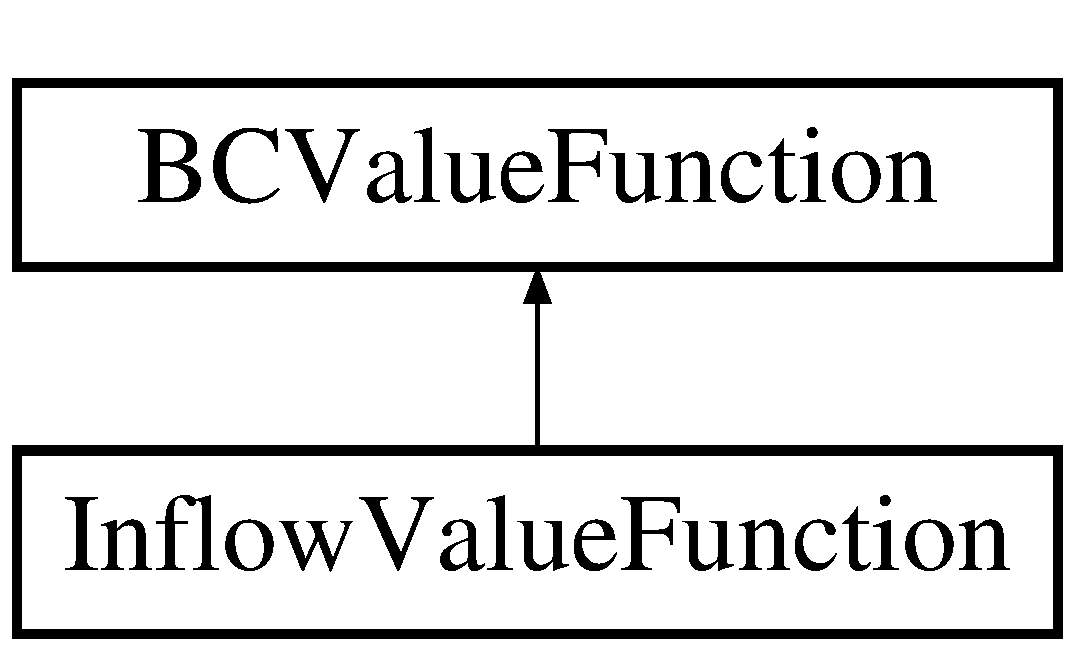
\includegraphics[height=2.000000cm]{class_inflow_value_function}
\end{center}
\end{figure}
\subsection*{Public Member Functions}
\begin{DoxyCompactItemize}
\item 
\hypertarget{class_inflow_value_function_aea9221992c346bbd12d03c3b7d86e47f}{\hyperlink{class_inflow_value_function_aea9221992c346bbd12d03c3b7d86e47f}{Inflow\-Value\-Function} ()}\label{class_inflow_value_function_aea9221992c346bbd12d03c3b7d86e47f}

\begin{DoxyCompactList}\small\item\em Default constructor. \end{DoxyCompactList}\item 
\hypertarget{class_inflow_value_function_a277df57c04250bc62a446a984a878546}{\hyperlink{class_inflow_value_function_a277df57c04250bc62a446a984a878546}{Inflow\-Value\-Function} (Real a\-\_\-value, int a\-\_\-n\-Comp, Real a\-\_\-inflow\-Value, Real a\-\_\-plume\-Start, Real a\-\_\-plume\-End)}\label{class_inflow_value_function_a277df57c04250bc62a446a984a878546}

\begin{DoxyCompactList}\small\item\em Constructor. \end{DoxyCompactList}\item 
\hypertarget{class_inflow_value_function_af9941db0cd9f74fc0a5133864cb7d141}{virtual void \hyperlink{class_inflow_value_function_af9941db0cd9f74fc0a5133864cb7d141}{operator()} (Real $\ast$a\-\_\-pos, int $\ast$a\-\_\-dir, Side\-::\-Lo\-Hi\-Side $\ast$a\-\_\-side, Real $\ast$a\-\_\-value)}\label{class_inflow_value_function_af9941db0cd9f74fc0a5133864cb7d141}

\begin{DoxyCompactList}\small\item\em Apply B\-C. \end{DoxyCompactList}\end{DoxyCompactItemize}
\subsection*{Public Attributes}
\begin{DoxyCompactItemize}
\item 
\hypertarget{class_inflow_value_function_a5a02392c298428969a7d750bbb111e80}{Real \hyperlink{class_inflow_value_function_a5a02392c298428969a7d750bbb111e80}{m\-\_\-value}}\label{class_inflow_value_function_a5a02392c298428969a7d750bbb111e80}

\begin{DoxyCompactList}\small\item\em The constant value to apply. \end{DoxyCompactList}\item 
\hypertarget{class_inflow_value_function_a5d9645cce1fdb3972fc7e2ae2b644b98}{int \hyperlink{class_inflow_value_function_a5d9645cce1fdb3972fc7e2ae2b644b98}{m\-\_\-n\-Comp}}\label{class_inflow_value_function_a5d9645cce1fdb3972fc7e2ae2b644b98}

\begin{DoxyCompactList}\small\item\em The component to apply this B\-C to. \end{DoxyCompactList}\item 
\hypertarget{class_inflow_value_function_a46bcf5848d66c489ac517d55259bfe44}{Real {\bfseries m\-\_\-inflow\-Value}}\label{class_inflow_value_function_a46bcf5848d66c489ac517d55259bfe44}

\item 
\hypertarget{class_inflow_value_function_a3e3686426aac78ec5aed2098e87f744c}{Real {\bfseries m\-\_\-plume\-Start}}\label{class_inflow_value_function_a3e3686426aac78ec5aed2098e87f744c}

\item 
\hypertarget{class_inflow_value_function_aa8f3be53977376cea300461c24e67e00}{Real {\bfseries m\-\_\-plume\-End}}\label{class_inflow_value_function_aa8f3be53977376cea300461c24e67e00}

\end{DoxyCompactItemize}


\subsection{Detailed Description}
Return one value for inflow, and another if not. 

The documentation for this class was generated from the following file\-:\begin{DoxyCompactItemize}
\item 
/home/parkinsonjl/mushy-\/layer/\-B\-Cutil/Phys\-B\-C\-Util.\-cpp\end{DoxyCompactItemize}

\hypertarget{class_level_advect}{\section{Level\-Advect Class Reference}
\label{class_level_advect}\index{Level\-Advect@{Level\-Advect}}
}


Advection integrator on a level.  




{\ttfamily \#include $<$Level\-Advect.\-H$>$}

\subsection*{Public Member Functions}
\begin{DoxyCompactItemize}
\item 
\hyperlink{class_level_advect_a87b0274e58afdb0058368ac6554592e5}{Level\-Advect} ()
\begin{DoxyCompactList}\small\item\em Default constructor. \end{DoxyCompactList}\item 
\hyperlink{class_level_advect_aeb34ed4774fb8e581789fd5a6ee2b4dd}{$\sim$\-Level\-Advect} ()
\begin{DoxyCompactList}\small\item\em Destructor. \end{DoxyCompactList}\item 
void \hyperlink{class_level_advect_aae945fee39376ceabd3fc46ea395e2fe}{define} (const Advect\-Physics \&a\-\_\-gphys, const Disjoint\-Box\-Layout \&a\-\_\-this\-Disjoint\-Box\-Layout, const Disjoint\-Box\-Layout \&a\-\_\-coarser\-Disjoint\-Box\-Layout, const Problem\-Domain \&a\-\_\-domain, const int \&a\-\_\-refine\-Coarse, const bool \&a\-\_\-use\-Limiting, const Real \&a\-\_\-dx, const bool \&a\-\_\-has\-Coarser, const bool \&a\-\_\-has\-Finer, const int \&a\-\_\-num\-Ghost)
\begin{DoxyCompactList}\small\item\em Actual constructor. \end{DoxyCompactList}\item 
Real \hyperlink{class_level_advect_a074ad96105762bb9796d642f07970c36}{step} (Level\-Data$<$ F\-Array\-Box $>$ \&a\-\_\-\-U, Level\-Flux\-Register \&a\-\_\-finer\-Flux\-Register, Level\-Flux\-Register \&a\-\_\-coarser\-Flux\-Register, Level\-Data$<$ Flux\-Box $>$ \&a\-\_\-advection\-Velocity, const Level\-Data$<$ F\-Array\-Box $>$ \&a\-\_\-\-S, const Level\-Data$<$ F\-Array\-Box $>$ \&a\-\_\-\-U\-Coarse\-Old, const Real \&a\-\_\-\-T\-Coarse\-Old, const Level\-Data$<$ F\-Array\-Box $>$ \&a\-\_\-\-U\-Coarse\-New, const Real \&a\-\_\-\-T\-Coarse\-New, const Real \&a\-\_\-time, const Real \&a\-\_\-dt, const bool a\-\_\-do\-F\-Rupdates=true, const bool a\-\_\-fill\-Ghosts=true)
\begin{DoxyCompactList}\small\item\em Advance the solution by one timestep on this grid level. \end{DoxyCompactList}\item 
void \hyperlink{class_level_advect_ab4af138371be3b5d2c4624b761e74941}{average\-Vel\-To\-C\-C} (F\-Array\-Box \&a\-\_\-normal\-Vel, const Flux\-Box \&a\-\_\-advection\-Vel, const Box \&a\-\_\-box) const 
\begin{DoxyCompactList}\small\item\em Convert velocity from face-\/centered to cell-\/centered. \end{DoxyCompactList}\item 
void \hyperlink{class_level_advect_a6e0534084ef26a19f41fbafe4bcba15e}{fill\-Ghost} (Level\-Data$<$ F\-Array\-Box $>$ \&a\-\_\-\-U, const Level\-Data$<$ F\-Array\-Box $>$ \&a\-\_\-\-U\-Coarse\-Old, const Real \&a\-\_\-\-T\-Coarse\-Old, const Level\-Data$<$ F\-Array\-Box $>$ \&a\-\_\-\-U\-Coarse\-New, const Real \&a\-\_\-\-T\-Coarse\-New, const Real \&a\-\_\-dt, const Real \&a\-\_\-time)
\begin{DoxyCompactList}\small\item\em Fill in ghost cells by exchange at this level and then by interpolation from coarser level (if any). \end{DoxyCompactList}\item 
Real \hyperlink{class_level_advect_a81626f8255195ae94d01248c3c90e6d5}{get\-Max\-Wave\-Speed} (const Level\-Data$<$ F\-Array\-Box $>$ \&a\-\_\-\-U, Level\-Data$<$ Flux\-Box $>$ \&a\-\_\-advection\-Velocity)
\begin{DoxyCompactList}\small\item\em Get maximum wave speed. \end{DoxyCompactList}\item 
\hypertarget{class_level_advect_a2dec4b6dd1075da650a811c8d0a32fe9}{void \hyperlink{class_level_advect_a2dec4b6dd1075da650a811c8d0a32fe9}{get\-Patch\-Godunov} (Patch\-Godunov \&patch\-Godunov)}\label{class_level_advect_a2dec4b6dd1075da650a811c8d0a32fe9}

\begin{DoxyCompactList}\small\item\em Get Patch\-Godunov object. \end{DoxyCompactList}\end{DoxyCompactItemize}
\subsection*{Protected Attributes}
\begin{DoxyCompactItemize}
\item 
\hypertarget{class_level_advect_a7e53aeeaa7bcd9e5371e5edf0a91956d}{Disjoint\-Box\-Layout \hyperlink{class_level_advect_a7e53aeeaa7bcd9e5371e5edf0a91956d}{m\-\_\-grids}}\label{class_level_advect_a7e53aeeaa7bcd9e5371e5edf0a91956d}

\begin{DoxyCompactList}\small\item\em layout for this level \end{DoxyCompactList}\item 
\hypertarget{class_level_advect_a5b9741fc6de32a21ea3dfa449288c6ac}{Patch\-Godunov \hyperlink{class_level_advect_a5b9741fc6de32a21ea3dfa449288c6ac}{m\-\_\-patch\-Godunov}}\label{class_level_advect_a5b9741fc6de32a21ea3dfa449288c6ac}

\begin{DoxyCompactList}\small\item\em patch integrator \end{DoxyCompactList}\item 
\hypertarget{class_level_advect_a26ff856333114236e82dbcfd712ba912}{Advect\-Physics $\ast$ \hyperlink{class_level_advect_a26ff856333114236e82dbcfd712ba912}{m\-\_\-advect\-Physics}}\label{class_level_advect_a26ff856333114236e82dbcfd712ba912}

\begin{DoxyCompactList}\small\item\em physics class \end{DoxyCompactList}\item 
\hypertarget{class_level_advect_a68fb9b1ed68cf6f6965e082e8f18e3ba}{int \hyperlink{class_level_advect_a68fb9b1ed68cf6f6965e082e8f18e3ba}{m\-\_\-num\-Ghost}}\label{class_level_advect_a68fb9b1ed68cf6f6965e082e8f18e3ba}

\begin{DoxyCompactList}\small\item\em number of ghost cells need locally for this level \end{DoxyCompactList}\item 
\hypertarget{class_level_advect_a752c22422040ef2e8b3d7e391155a0a7}{Copier \hyperlink{class_level_advect_a752c22422040ef2e8b3d7e391155a0a7}{m\-\_\-exchange\-Copier}}\label{class_level_advect_a752c22422040ef2e8b3d7e391155a0a7}

\begin{DoxyCompactList}\small\item\em exchange copier \end{DoxyCompactList}\item 
\hypertarget{class_level_advect_a5719da936000c1a7e4dcffc9d43aaf97}{Piecewise\-Linear\-Fill\-Patch \hyperlink{class_level_advect_a5719da936000c1a7e4dcffc9d43aaf97}{m\-\_\-patcher}}\label{class_level_advect_a5719da936000c1a7e4dcffc9d43aaf97}

\begin{DoxyCompactList}\small\item\em interpolator for filling in ghost cells from the next coarser level \end{DoxyCompactList}\item 
\hypertarget{class_level_advect_a3ee22e9a3df1f1c2400e6fd989158922}{Real \hyperlink{class_level_advect_a3ee22e9a3df1f1c2400e6fd989158922}{m\-\_\-dx}}\label{class_level_advect_a3ee22e9a3df1f1c2400e6fd989158922}

\begin{DoxyCompactList}\small\item\em grid spacing \end{DoxyCompactList}\item 
\hypertarget{class_level_advect_acc95fd3bf2296642ceb3cd97e733ac41}{Problem\-Domain \hyperlink{class_level_advect_acc95fd3bf2296642ceb3cd97e733ac41}{m\-\_\-domain}}\label{class_level_advect_acc95fd3bf2296642ceb3cd97e733ac41}

\begin{DoxyCompactList}\small\item\em problem domain -\/ index space for this level \end{DoxyCompactList}\item 
\hypertarget{class_level_advect_aba7ddca5882201cdbab13efc47e8635c}{int \hyperlink{class_level_advect_aba7ddca5882201cdbab13efc47e8635c}{m\-\_\-refine\-Coarse}}\label{class_level_advect_aba7ddca5882201cdbab13efc47e8635c}

\begin{DoxyCompactList}\small\item\em refinement ratio between this level and the next coarser \end{DoxyCompactList}\item 
\hypertarget{class_level_advect_a4c6b16c657ec5bf5053dfeae3dae64c0}{bool \hyperlink{class_level_advect_a4c6b16c657ec5bf5053dfeae3dae64c0}{m\-\_\-has\-Coarser}}\label{class_level_advect_a4c6b16c657ec5bf5053dfeae3dae64c0}

\begin{DoxyCompactList}\small\item\em whether a coarser level exists \end{DoxyCompactList}\item 
\hypertarget{class_level_advect_a71f2193804df1cdb778e7f8f98eb05d0}{bool \hyperlink{class_level_advect_a71f2193804df1cdb778e7f8f98eb05d0}{m\-\_\-has\-Finer}}\label{class_level_advect_a71f2193804df1cdb778e7f8f98eb05d0}

\begin{DoxyCompactList}\small\item\em whether a finer level exists \end{DoxyCompactList}\item 
\hypertarget{class_level_advect_a8a72b368d22f9f10fa9366365038a9bb}{int \hyperlink{class_level_advect_a8a72b368d22f9f10fa9366365038a9bb}{m\-\_\-num\-Cons}}\label{class_level_advect_a8a72b368d22f9f10fa9366365038a9bb}

\begin{DoxyCompactList}\small\item\em number of conserved variables (= 1) \end{DoxyCompactList}\item 
\hypertarget{class_level_advect_a554f4194c313e68690e2eaf3bd405630}{int \hyperlink{class_level_advect_a554f4194c313e68690e2eaf3bd405630}{m\-\_\-normal\-Pred\-Order}}\label{class_level_advect_a554f4194c313e68690e2eaf3bd405630}

\begin{DoxyCompactList}\small\item\em order of normal predictor \end{DoxyCompactList}\item 
\hypertarget{class_level_advect_a1eb9a05109cd588504185e3c5ee360af}{bool \hyperlink{class_level_advect_a1eb9a05109cd588504185e3c5ee360af}{m\-\_\-use\-Fourth\-Order\-Slopes}}\label{class_level_advect_a1eb9a05109cd588504185e3c5ee360af}

\begin{DoxyCompactList}\small\item\em whether to use 4th-\/order slope computations (otherwise, use 2nd order) \end{DoxyCompactList}\item 
\hypertarget{class_level_advect_ac75d3b654493d0b22955e9c573449089}{bool \hyperlink{class_level_advect_ac75d3b654493d0b22955e9c573449089}{m\-\_\-use\-Prim\-Limiting}}\label{class_level_advect_ac75d3b654493d0b22955e9c573449089}

\begin{DoxyCompactList}\small\item\em whether to do slope limiting in the primitive variables \end{DoxyCompactList}\item 
\hypertarget{class_level_advect_a586ff8dcb0832298bd962d061eb4ef56}{bool \hyperlink{class_level_advect_a586ff8dcb0832298bd962d061eb4ef56}{m\-\_\-use\-Char\-Limiting}}\label{class_level_advect_a586ff8dcb0832298bd962d061eb4ef56}

\begin{DoxyCompactList}\small\item\em whether to do slope limiting in the characteristic variables \end{DoxyCompactList}\item 
\hypertarget{class_level_advect_a14bfed42bbb2388494f60443ec92d4db}{bool \hyperlink{class_level_advect_a14bfed42bbb2388494f60443ec92d4db}{m\-\_\-use\-Flattening}}\label{class_level_advect_a14bfed42bbb2388494f60443ec92d4db}

\begin{DoxyCompactList}\small\item\em whether to do slope flattening -\/ M\-U\-S\-T B\-E U\-S\-I\-N\-G 4th-\/order slopes \end{DoxyCompactList}\item 
\hypertarget{class_level_advect_a3971ab078e31ce2d6815e813583804a5}{bool \hyperlink{class_level_advect_a3971ab078e31ce2d6815e813583804a5}{m\-\_\-use\-Artificial\-Viscosity}}\label{class_level_advect_a3971ab078e31ce2d6815e813583804a5}

\begin{DoxyCompactList}\small\item\em whether to apply artificial viscosity of a set value \end{DoxyCompactList}\item 
\hypertarget{class_level_advect_a3555480c3e66811829d48d3ace711dbc}{Real \hyperlink{class_level_advect_a3555480c3e66811829d48d3ace711dbc}{m\-\_\-artificial\-Viscosity}}\label{class_level_advect_a3555480c3e66811829d48d3ace711dbc}

\begin{DoxyCompactList}\small\item\em artificial viscosity coefficient \end{DoxyCompactList}\item 
\hypertarget{class_level_advect_a3f6eda4ee5c690fa4c2ca76404510f0a}{bool \hyperlink{class_level_advect_a3f6eda4ee5c690fa4c2ca76404510f0a}{m\-\_\-is\-Defined}}\label{class_level_advect_a3f6eda4ee5c690fa4c2ca76404510f0a}

\begin{DoxyCompactList}\small\item\em whether this object has been defined \end{DoxyCompactList}\end{DoxyCompactItemize}


\subsection{Detailed Description}
Advection integrator on a level. 

\subsection{Constructor \& Destructor Documentation}
\hypertarget{class_level_advect_a87b0274e58afdb0058368ac6554592e5}{\index{Level\-Advect@{Level\-Advect}!Level\-Advect@{Level\-Advect}}
\index{Level\-Advect@{Level\-Advect}!LevelAdvect@{Level\-Advect}}
\subsubsection[{Level\-Advect}]{\setlength{\rightskip}{0pt plus 5cm}Level\-Advect\-::\-Level\-Advect (
\begin{DoxyParamCaption}
{}
\end{DoxyParamCaption}
)\hspace{0.3cm}{\ttfamily [inline]}}}\label{class_level_advect_a87b0274e58afdb0058368ac6554592e5}


Default constructor. 

Object requires \hyperlink{class_level_advect_aae945fee39376ceabd3fc46ea395e2fe}{define()} to be called before all other functions. \hypertarget{class_level_advect_aeb34ed4774fb8e581789fd5a6ee2b4dd}{\index{Level\-Advect@{Level\-Advect}!$\sim$\-Level\-Advect@{$\sim$\-Level\-Advect}}
\index{$\sim$\-Level\-Advect@{$\sim$\-Level\-Advect}!LevelAdvect@{Level\-Advect}}
\subsubsection[{$\sim$\-Level\-Advect}]{\setlength{\rightskip}{0pt plus 5cm}Level\-Advect\-::$\sim$\-Level\-Advect (
\begin{DoxyParamCaption}
{}
\end{DoxyParamCaption}
)\hspace{0.3cm}{\ttfamily [inline]}}}\label{class_level_advect_aeb34ed4774fb8e581789fd5a6ee2b4dd}


Destructor. 

Destroys all objects created by \hyperlink{class_level_advect_aae945fee39376ceabd3fc46ea395e2fe}{define()}. Passed in data references of \hyperlink{class_level_advect_aae945fee39376ceabd3fc46ea395e2fe}{define()} are left alone. 

\subsection{Member Function Documentation}
\hypertarget{class_level_advect_ab4af138371be3b5d2c4624b761e74941}{\index{Level\-Advect@{Level\-Advect}!average\-Vel\-To\-C\-C@{average\-Vel\-To\-C\-C}}
\index{average\-Vel\-To\-C\-C@{average\-Vel\-To\-C\-C}!LevelAdvect@{Level\-Advect}}
\subsubsection[{average\-Vel\-To\-C\-C}]{\setlength{\rightskip}{0pt plus 5cm}void Level\-Advect\-::average\-Vel\-To\-C\-C (
\begin{DoxyParamCaption}
\item[{F\-Array\-Box \&}]{a\-\_\-normal\-Vel, }
\item[{const Flux\-Box \&}]{a\-\_\-advection\-Vel, }
\item[{const Box \&}]{a\-\_\-box}
\end{DoxyParamCaption}
) const}}\label{class_level_advect_ab4af138371be3b5d2c4624b761e74941}


Convert velocity from face-\/centered to cell-\/centered. 

In each direction, take average of normal component of velocity on the neighboring faces in that direction. 
\begin{DoxyParams}{Parameters}
{\em a\-\_\-normal\-Vel} & cell-\/centered velocity \\
\hline
{\em a\-\_\-advection\-Vel} & face-\/centered velocity \\
\hline
{\em a\-\_\-box} & Box on which to return a\-\_\-normal\-Vel \\
\hline
\end{DoxyParams}
\hypertarget{class_level_advect_aae945fee39376ceabd3fc46ea395e2fe}{\index{Level\-Advect@{Level\-Advect}!define@{define}}
\index{define@{define}!LevelAdvect@{Level\-Advect}}
\subsubsection[{define}]{\setlength{\rightskip}{0pt plus 5cm}void Level\-Advect\-::define (
\begin{DoxyParamCaption}
\item[{const Advect\-Physics \&}]{a\-\_\-gphys, }
\item[{const Disjoint\-Box\-Layout \&}]{a\-\_\-this\-Disjoint\-Box\-Layout, }
\item[{const Disjoint\-Box\-Layout \&}]{a\-\_\-coarser\-Disjoint\-Box\-Layout, }
\item[{const Problem\-Domain \&}]{a\-\_\-domain, }
\item[{const int \&}]{a\-\_\-refine\-Coarse, }
\item[{const bool \&}]{a\-\_\-use\-Limiting, }
\item[{const Real \&}]{a\-\_\-dx, }
\item[{const bool \&}]{a\-\_\-has\-Coarser, }
\item[{const bool \&}]{a\-\_\-has\-Finer, }
\item[{const int \&}]{a\-\_\-num\-Ghost}
\end{DoxyParamCaption}
)}}\label{class_level_advect_aae945fee39376ceabd3fc46ea395e2fe}


Actual constructor. 

Inside the routine, we cast away const-\/ness on the data members for the assignment. The arguments passed in are maintained const (coding standards). 
\begin{DoxyParams}{Parameters}
{\em a\-\_\-gphys} & advection physics class \\
\hline
{\em a\-\_\-this\-Disjoint\-Box\-Layout} & box layout at this level \\
\hline
{\em a\-\_\-coarser\-Disjoint\-Box\-Layout} & box layout at next coarser level (or empty if this is coarsest level) \\
\hline
{\em a\-\_\-domain} & problem domain at this level \\
\hline
{\em a\-\_\-refine\-Coarse} & refinement ratio between this level and next coarser level \\
\hline
{\em a\-\_\-use\-Limiting} & whether to use limiting \\
\hline
{\em a\-\_\-dx} & grid spacing at this level \\
\hline
{\em a\-\_\-has\-Coarser} & whether there is a coarser level \\
\hline
{\em a\-\_\-has\-Finer} & whether there is a finer level \\
\hline
{\em a\-\_\-num\-Ghost} & number of ghost cells \\
\hline
\end{DoxyParams}
\hypertarget{class_level_advect_a6e0534084ef26a19f41fbafe4bcba15e}{\index{Level\-Advect@{Level\-Advect}!fill\-Ghost@{fill\-Ghost}}
\index{fill\-Ghost@{fill\-Ghost}!LevelAdvect@{Level\-Advect}}
\subsubsection[{fill\-Ghost}]{\setlength{\rightskip}{0pt plus 5cm}void Level\-Advect\-::fill\-Ghost (
\begin{DoxyParamCaption}
\item[{Level\-Data$<$ F\-Array\-Box $>$ \&}]{a\-\_\-\-U, }
\item[{const Level\-Data$<$ F\-Array\-Box $>$ \&}]{a\-\_\-\-U\-Coarse\-Old, }
\item[{const Real \&}]{a\-\_\-\-T\-Coarse\-Old, }
\item[{const Level\-Data$<$ F\-Array\-Box $>$ \&}]{a\-\_\-\-U\-Coarse\-New, }
\item[{const Real \&}]{a\-\_\-\-T\-Coarse\-New, }
\item[{const Real \&}]{a\-\_\-dt, }
\item[{const Real \&}]{a\-\_\-time}
\end{DoxyParamCaption}
)}}\label{class_level_advect_a6e0534084ef26a19f41fbafe4bcba15e}


Fill in ghost cells by exchange at this level and then by interpolation from coarser level (if any). 


\begin{DoxyParams}{Parameters}
{\em a\-\_\-\-U} & conserved variables at this level, with ghosts cells to be filled in \\
\hline
{\em a\-\_\-\-U\-Coarse\-Old} & conserved variables at coarser level at time of last coarser-\/level update, or empty if no coarser level; may be empty if interpolation not required \\
\hline
{\em a\-\_\-\-T\-Coarse\-Old} & time of last update at coarser level \\
\hline
{\em a\-\_\-\-U\-Coarse\-New} & conserved variables at coarser level at time of next coarser-\/level update, or empty if no coarser level; may be empty if interpolation not required \\
\hline
{\em a\-\_\-\-T\-Coarse\-New} & time of next update at coarser level \\
\hline
{\em a\-\_\-dt} & time step \\
\hline
{\em a\-\_\-time} & current time \\
\hline
\end{DoxyParams}
\hypertarget{class_level_advect_a81626f8255195ae94d01248c3c90e6d5}{\index{Level\-Advect@{Level\-Advect}!get\-Max\-Wave\-Speed@{get\-Max\-Wave\-Speed}}
\index{get\-Max\-Wave\-Speed@{get\-Max\-Wave\-Speed}!LevelAdvect@{Level\-Advect}}
\subsubsection[{get\-Max\-Wave\-Speed}]{\setlength{\rightskip}{0pt plus 5cm}Real Level\-Advect\-::get\-Max\-Wave\-Speed (
\begin{DoxyParamCaption}
\item[{const Level\-Data$<$ F\-Array\-Box $>$ \&}]{a\-\_\-\-U, }
\item[{Level\-Data$<$ Flux\-Box $>$ \&}]{a\-\_\-advection\-Velocity}
\end{DoxyParamCaption}
)}}\label{class_level_advect_a81626f8255195ae94d01248c3c90e6d5}


Get maximum wave speed. 


\begin{DoxyParams}{Parameters}
{\em a\-\_\-\-U} & conserved variables at this level \\
\hline
{\em a\-\_\-advection\-Velocity} & face-\/centered velocities \\
\hline
\end{DoxyParams}
\hypertarget{class_level_advect_a074ad96105762bb9796d642f07970c36}{\index{Level\-Advect@{Level\-Advect}!step@{step}}
\index{step@{step}!LevelAdvect@{Level\-Advect}}
\subsubsection[{step}]{\setlength{\rightskip}{0pt plus 5cm}Real Level\-Advect\-::step (
\begin{DoxyParamCaption}
\item[{Level\-Data$<$ F\-Array\-Box $>$ \&}]{a\-\_\-\-U, }
\item[{Level\-Flux\-Register \&}]{a\-\_\-finer\-Flux\-Register, }
\item[{Level\-Flux\-Register \&}]{a\-\_\-coarser\-Flux\-Register, }
\item[{Level\-Data$<$ Flux\-Box $>$ \&}]{a\-\_\-advection\-Velocity, }
\item[{const Level\-Data$<$ F\-Array\-Box $>$ \&}]{a\-\_\-\-S, }
\item[{const Level\-Data$<$ F\-Array\-Box $>$ \&}]{a\-\_\-\-U\-Coarse\-Old, }
\item[{const Real \&}]{a\-\_\-\-T\-Coarse\-Old, }
\item[{const Level\-Data$<$ F\-Array\-Box $>$ \&}]{a\-\_\-\-U\-Coarse\-New, }
\item[{const Real \&}]{a\-\_\-\-T\-Coarse\-New, }
\item[{const Real \&}]{a\-\_\-time, }
\item[{const Real \&}]{a\-\_\-dt, }
\item[{const bool}]{a\-\_\-do\-F\-Rupdates = {\ttfamily true}, }
\item[{const bool}]{a\-\_\-fill\-Ghosts = {\ttfamily true}}
\end{DoxyParamCaption}
)}}\label{class_level_advect_a074ad96105762bb9796d642f07970c36}


Advance the solution by one timestep on this grid level. 


\begin{DoxyParams}{Parameters}
{\em a\-\_\-\-U} & conserved variables at this level, defined on a\-\_\-this\-Disjoint\-Box\-Layout in \hyperlink{class_level_advect_aae945fee39376ceabd3fc46ea395e2fe}{define()}; gets updated in this routine \\
\hline
{\em a\-\_\-finer\-Flux\-Register} & flux register with next finer level \\
\hline
{\em a\-\_\-coarser\-Flux\-Register} & flux register with next coarser level \\
\hline
{\em a\-\_\-advection\-Velocity} & advection velocity on faces \\
\hline
{\em a\-\_\-\-S} & source term, or if no source term then this is null constructed and not defined \\
\hline
{\em a\-\_\-\-U\-Coarse\-Old} & conserved variables at coarser level at time of last coarser-\/level update, or empty if no coarser level; may be empty if interpolation not required \\
\hline
{\em a\-\_\-\-T\-Coarse\-Old} & time of last update at coarser level \\
\hline
{\em a\-\_\-\-U\-Coarse\-New} & conserved variables at coarser level at time of next coarser-\/level update, or empty if no coarser level; may be empty if interpolation not required \\
\hline
{\em a\-\_\-\-T\-Coarse\-New} & time of next update at coarser level \\
\hline
{\em a\-\_\-time} & current time \\
\hline
{\em a\-\_\-dt} & time step \\
\hline
{\em a\-\_\-do\-F\-Rupdates} & whether or not to do flux register updates \\
\hline
{\em a\-\_\-fill\-Ghosts} & whether or not to fill ghost cells \\
\hline
\end{DoxyParams}


The documentation for this class was generated from the following files\-:\begin{DoxyCompactItemize}
\item 
/home/parkinsonjl/mushy-\/layer/src/Level\-Advect.\-H\item 
/home/parkinsonjl/mushy-\/layer/src/Level\-Advect.\-cpp\end{DoxyCompactItemize}

\hypertarget{class_mask}{\section{Mask Class Reference}
\label{class_mask}\index{Mask@{Mask}}
}


class to determine coarse-\/fine validity info  




{\ttfamily \#include $<$Mask.\-H$>$}

\subsection*{Public Types}
\begin{DoxyCompactItemize}
\item 
enum \hyperlink{class_mask_a81350474ba1eed5e378837d0772d86c2}{cell\-Type} \{ {\bfseries mask\-Covered} = -\/2, 
{\bfseries mask\-Physical} = -\/1, 
{\bfseries mask\-Copy} = 0, 
{\bfseries mask\-Coarse} = 1
 \}
\begin{DoxyCompactList}\small\item\em Cell type. \end{DoxyCompactList}\end{DoxyCompactItemize}
\subsection*{Public Member Functions}
\begin{DoxyCompactItemize}
\item 
\hypertarget{class_mask_ab1652414426159d30e756e1da3a8932c}{void \hyperlink{class_mask_ab1652414426159d30e756e1da3a8932c}{build\-Mask} (Base\-Fab$<$ int $>$ \&a\-\_\-mask, const Problem\-Domain \&a\-\_\-d\-Problem, const Box\-Layout \&a\-\_\-grids, const Box\-Layout $\ast$a\-\_\-fine\-Grids\-Ptr=N\-U\-L\-L, int a\-\_\-n\-Ref\-Fine=-\/1)}\label{class_mask_ab1652414426159d30e756e1da3a8932c}

\begin{DoxyCompactList}\small\item\em Build mask. \end{DoxyCompactList}\item 
\hypertarget{class_mask_a2d53aed5c96ff103c2b54955a134c5af}{void \hyperlink{class_mask_a2d53aed5c96ff103c2b54955a134c5af}{build\-Masks} (Level\-Data$<$ Base\-Fab$<$ int $>$ $>$ \&a\-\_\-masks, const Problem\-Domain \&a\-\_\-d\-Problem, const Box\-Layout \&a\-\_\-grids, const Box\-Layout $\ast$a\-\_\-fine\-Grids\-Ptr=N\-U\-L\-L, int a\-\_\-n\-Ref\-Fine=-\/1)}\label{class_mask_a2d53aed5c96ff103c2b54955a134c5af}

\begin{DoxyCompactList}\small\item\em Build masks. \end{DoxyCompactList}\item 
\hypertarget{class_mask_a5df266dd84059e03b3e1e139c98c6c66}{void \hyperlink{class_mask_a5df266dd84059e03b3e1e139c98c6c66}{build\-Mask} (Base\-Fab$<$ int $>$ \&a\-\_\-mask, const Box \&a\-\_\-d\-Problem, const Box\-Layout \&a\-\_\-grids, const Box\-Layout $\ast$a\-\_\-fine\-Grids\-Ptr=N\-U\-L\-L, int a\-\_\-n\-Ref\-Fine=-\/1)}\label{class_mask_a5df266dd84059e03b3e1e139c98c6c66}

\begin{DoxyCompactList}\small\item\em deprecated interface \end{DoxyCompactList}\item 
\hypertarget{class_mask_ac62bddb04af6dbbe798a870a1e86c01c}{void \hyperlink{class_mask_ac62bddb04af6dbbe798a870a1e86c01c}{build\-Masks} (Level\-Data$<$ Base\-Fab$<$ int $>$ $>$ \&a\-\_\-masks, const Box \&a\-\_\-d\-Problem, const Box\-Layout \&a\-\_\-grids, const Box\-Layout $\ast$a\-\_\-fine\-Grids\-Ptr=N\-U\-L\-L, int a\-\_\-n\-Ref\-Fine=-\/1)}\label{class_mask_ac62bddb04af6dbbe798a870a1e86c01c}

\begin{DoxyCompactList}\small\item\em deprecated interface \end{DoxyCompactList}\end{DoxyCompactItemize}


\subsection{Detailed Description}
class to determine coarse-\/fine validity info 

The documentation for this class was generated from the following files\-:\begin{DoxyCompactItemize}
\item 
/home/parkinsonjl/mushy-\/layer/util/Mask.\-H\item 
/home/parkinsonjl/mushy-\/layer/util/Mask.\-cpp\end{DoxyCompactItemize}

\hypertarget{class_mushy_layer_params}{\section{Mushy\-Layer\-Params Class Reference}
\label{class_mushy_layer_params}\index{Mushy\-Layer\-Params@{Mushy\-Layer\-Params}}
}


Class to handle the physical parameters of a mushy layer simulation.  




{\ttfamily \#include $<$Mushy\-Layer\-Params.\-h$>$}

\subsection*{Public Types}
\begin{DoxyCompactItemize}
\item 
enum {\bfseries nondimensionalisations} \{ \\*
{\bfseries m\-\_\-diffusive\-Time\-\_\-advective\-Vel}, 
{\bfseries m\-\_\-darcy\-Time\-\_\-advective\-Vel}, 
{\bfseries m\-\_\-darcy\-Time\-\_\-darcy\-Vel}, 
{\bfseries m\-\_\-advective\-Time\-\_\-darcy\-Vel}, 
\\*
{\bfseries m\-\_\-buoyancy\-Time\-\_\-advective\-Vel}, 
{\bfseries m\-\_\-num\-\_\-nondimensionalisations}
 \}
\item 
enum \hyperlink{class_mushy_layer_params_a029cd583b3d31671363f600177a885ac}{time\-Dependent\-B\-Ctypes} \{ {\bfseries m\-\_\-constant}, 
{\bfseries m\-\_\-sinusoid}, 
{\bfseries m\-\_\-custom}
 \}
\begin{DoxyCompactList}\small\item\em Possible time dependences for B\-Cs. \end{DoxyCompactList}\item 
enum \hyperlink{class_mushy_layer_params_aed4f8585e71acda083351ecdc6be5b5c}{permeability\-Functions} \{ \\*
{\bfseries m\-\_\-pure\-Fluid}, 
{\bfseries m\-\_\-cubic\-Permeability}, 
{\bfseries m\-\_\-kozeny\-Carman}, 
{\bfseries m\-\_\-log\-Permeability}, 
\\*
{\bfseries m\-\_\-permeability\-X\-Squared}, 
{\bfseries m\-\_\-porosity\-Permeability}
 \}
\begin{DoxyCompactList}\small\item\em Different possible permeability functions. \end{DoxyCompactList}\item 
enum {\bfseries porosity\-Functions} \{ \\*
{\bfseries m\-\_\-porosity\-Constant}, 
{\bfseries m\-\_\-porosity\-Linear}, 
{\bfseries m\-\_\-porosity\-Gaussian}, 
{\bfseries m\-\_\-porosity\-Edge}, 
\\*
{\bfseries m\-\_\-porosity\-Time\-Dependent}
 \}
\item 
enum \hyperlink{class_mushy_layer_params_a9681d6bd2a80ea8862f8e5442a403309}{physical\-Problems} \{ \\*
{\bfseries m\-\_\-mushy\-Layer}, 
{\bfseries m\-\_\-burgers\-Sin}, 
{\bfseries m\-\_\-burgers\-Periodic}, 
{\bfseries m\-\_\-poiseuille\-Flow}, 
\\*
{\bfseries m\-\_\-diffusion}, 
{\bfseries m\-\_\-solidification\-No\-Flow}, 
{\bfseries m\-\_\-corner\-Flow}, 
{\bfseries m\-\_\-sidewall\-Heating}, 
\\*
{\bfseries m\-\_\-\-H\-R\-L}, 
{\bfseries m\-\_\-rayleigh\-Benard}, 
{\bfseries m\-\_\-solute\-Flux\-Test}, 
{\bfseries m\-\_\-reflux\-Test}, 
\\*
{\bfseries m\-\_\-zero\-Porosity\-Test}, 
{\bfseries m\-\_\-melting\-Ice\-Block}, 
{\bfseries m\-\_\-convection\-Mixed\-Porous}, 
{\bfseries m\-\_\-vortex\-Pair}
 \}
\begin{DoxyCompactList}\small\item\em Different physical problems. \end{DoxyCompactList}\end{DoxyCompactItemize}
\subsection*{Public Member Functions}
\begin{DoxyCompactItemize}
\item 
\hypertarget{class_mushy_layer_params_a2adf3cf11a6d85e97d1bd05d21e0fda0}{void \hyperlink{class_mushy_layer_params_a2adf3cf11a6d85e97d1bd05d21e0fda0}{get\-Parameters} ()}\label{class_mushy_layer_params_a2adf3cf11a6d85e97d1bd05d21e0fda0}

\begin{DoxyCompactList}\small\item\em Get all parameters from the inputs file. \end{DoxyCompactList}\item 
\hypertarget{class_mushy_layer_params_ab0c7b6204884af8093216788b3d1635f}{void \hyperlink{class_mushy_layer_params_ab0c7b6204884af8093216788b3d1635f}{print\-Parameters} ()}\label{class_mushy_layer_params_ab0c7b6204884af8093216788b3d1635f}

\begin{DoxyCompactList}\small\item\em Write out parameters to the command line (pout) \end{DoxyCompactList}\item 
\hypertarget{class_mushy_layer_params_a63bfa2c38942a3113a2cd99c694c003b}{Real \hyperlink{class_mushy_layer_params_a63bfa2c38942a3113a2cd99c694c003b}{directional\-Solidification\-Mushy\-Z} (Real theta, Real z\-Eutectic=1.\-0)}\label{class_mushy_layer_params_a63bfa2c38942a3113a2cd99c694c003b}

\begin{DoxyCompactList}\small\item\em Calculate $ z(\theta) $ for the directional solidification without flow benchmark. \end{DoxyCompactList}\item 
\hypertarget{class_mushy_layer_params_a497dc7bd7c29819bd697d255af8de3d6}{void \hyperlink{class_mushy_layer_params_a497dc7bd7c29819bd697d255af8de3d6}{parse\-B\-Cs} (string a\-\_\-name, Vector$<$ int $>$ $\ast$a\-\_\-bc\-Holder, bool required=false)}\label{class_mushy_layer_params_a497dc7bd7c29819bd697d255af8de3d6}

\begin{DoxyCompactList}\small\item\em Read in B\-Cs from the inputs file. \end{DoxyCompactList}\item 
\hypertarget{class_mushy_layer_params_a534c1e576d710007d5bb7ad8354cd495}{void \hyperlink{class_mushy_layer_params_a534c1e576d710007d5bb7ad8354cd495}{parse\-B\-C\-Vals} (string a\-\_\-name, Real\-Vect \&a\-\_\-bc\-Holder, bool required=false)}\label{class_mushy_layer_params_a534c1e576d710007d5bb7ad8354cd495}

\begin{DoxyCompactList}\small\item\em Read in B\-C vals from inputs file. \end{DoxyCompactList}\item 
\hypertarget{class_mushy_layer_params_a096f90c939815ffda795d7c81a0a25d3}{Real \hyperlink{class_mushy_layer_params_a096f90c939815ffda795d7c81a0a25d3}{temp\-Totheta} (const Real T)}\label{class_mushy_layer_params_a096f90c939815ffda795d7c81a0a25d3}

\begin{DoxyCompactList}\small\item\em Convert dimensional to non-\/dimensional temperature. \end{DoxyCompactList}\item 
\hypertarget{class_mushy_layer_params_ab9cc390b6c5db5c4d6f083c0f2f14503}{Real \hyperlink{class_mushy_layer_params_ab9cc390b6c5db5c4d6f083c0f2f14503}{conc\-To\-Theta} (const Real C)}\label{class_mushy_layer_params_ab9cc390b6c5db5c4d6f083c0f2f14503}

\begin{DoxyCompactList}\small\item\em Convert dimensional to non-\/dimensional composition. \end{DoxyCompactList}\item 
\hypertarget{class_mushy_layer_params_ae036d6b6250a955546827dd17b9f967c}{int \hyperlink{class_mushy_layer_params_ae036d6b6250a955546827dd17b9f967c}{get\-Vel\-B\-C\-Type} (int dir, Side\-::\-Lo\-Hi\-Side side)}\label{class_mushy_layer_params_ae036d6b6250a955546827dd17b9f967c}

\begin{DoxyCompactList}\small\item\em Get the velocity boundary condition. \end{DoxyCompactList}\item 
\hypertarget{class_mushy_layer_params_a4b241acadb703afb0034a7bc39bdce00}{Real \hyperlink{class_mushy_layer_params_a4b241acadb703afb0034a7bc39bdce00}{calculate\-Permeability} (Real liquid\-Fraction)}\label{class_mushy_layer_params_a4b241acadb703afb0034a7bc39bdce00}

\begin{DoxyCompactList}\small\item\em Compute permeability from porosity. \end{DoxyCompactList}\item 
\hypertarget{class_mushy_layer_params_ab026a06d59c128d23f360e83cbd41eaa}{void \hyperlink{class_mushy_layer_params_ab026a06d59c128d23f360e83cbd41eaa}{set\-Time} (Real a\-\_\-time)}\label{class_mushy_layer_params_ab026a06d59c128d23f360e83cbd41eaa}

\begin{DoxyCompactList}\small\item\em Set the time, might be used for B\-Cs. \end{DoxyCompactList}\end{DoxyCompactItemize}
\subsection*{Public Attributes}
\begin{DoxyCompactItemize}
\item 
\hypertarget{class_mushy_layer_params_ab3689b3bc343632d15684e88c48f2278}{int \hyperlink{class_mushy_layer_params_ab3689b3bc343632d15684e88c48f2278}{physical\-Problem}}\label{class_mushy_layer_params_ab3689b3bc343632d15684e88c48f2278}

\begin{DoxyCompactList}\small\item\em Benchmark problem to solve. \end{DoxyCompactList}\item 
\hypertarget{class_mushy_layer_params_a0458bb90fd4db3977b2af0a0aa369386}{Real \hyperlink{class_mushy_layer_params_a0458bb90fd4db3977b2af0a0aa369386}{viscosity}}\label{class_mushy_layer_params_a0458bb90fd4db3977b2af0a0aa369386}

\begin{DoxyCompactList}\small\item\em Viscosity, $ \eta $, used in rayleigh number calculations. \end{DoxyCompactList}\item 
\hypertarget{class_mushy_layer_params_ac5dcaee57b4ea4ea4fc1c26d578f2e48}{Real \hyperlink{class_mushy_layer_params_ac5dcaee57b4ea4ea4fc1c26d578f2e48}{heat\-Conductivity\-Liquid}}\label{class_mushy_layer_params_ac5dcaee57b4ea4ea4fc1c26d578f2e48}

\begin{DoxyCompactList}\small\item\em Liquid heat conductivity, $ k_l $. \end{DoxyCompactList}\item 
\hypertarget{class_mushy_layer_params_a57cd61cc35cfd06330a3cb6e67c1bddc}{Real \hyperlink{class_mushy_layer_params_a57cd61cc35cfd06330a3cb6e67c1bddc}{heat\-Conductivity\-Solid}}\label{class_mushy_layer_params_a57cd61cc35cfd06330a3cb6e67c1bddc}

\begin{DoxyCompactList}\small\item\em Solid heat conductivity, $ k_s $. \end{DoxyCompactList}\item 
\hypertarget{class_mushy_layer_params_ab80de1952111d2c7bd8eeb30c4388441}{Real \hyperlink{class_mushy_layer_params_ab80de1952111d2c7bd8eeb30c4388441}{specific\-Heat\-Liquid}}\label{class_mushy_layer_params_ab80de1952111d2c7bd8eeb30c4388441}

\begin{DoxyCompactList}\small\item\em Specific heat capacity of the liquid phase, $ c_l $. \end{DoxyCompactList}\item 
\hypertarget{class_mushy_layer_params_ad7f89d49eb18122b9a8a6be3359ae5c1}{Real \hyperlink{class_mushy_layer_params_ad7f89d49eb18122b9a8a6be3359ae5c1}{specific\-Heat\-Solid}}\label{class_mushy_layer_params_ad7f89d49eb18122b9a8a6be3359ae5c1}

\begin{DoxyCompactList}\small\item\em Specific heat capacity of the solid phase, $c_s$. \end{DoxyCompactList}\item 
\hypertarget{class_mushy_layer_params_add77a2b935f21ac4cf3d7fe83afac04c}{Real \hyperlink{class_mushy_layer_params_add77a2b935f21ac4cf3d7fe83afac04c}{liquid\-Density}}\label{class_mushy_layer_params_add77a2b935f21ac4cf3d7fe83afac04c}

\begin{DoxyCompactList}\small\item\em Density of the liquid. \end{DoxyCompactList}\item 
\hypertarget{class_mushy_layer_params_a98ffdd6b098c0950601611df2b6c60a4}{Real \hyperlink{class_mushy_layer_params_a98ffdd6b098c0950601611df2b6c60a4}{latent\-Heat\-Dissolution}}\label{class_mushy_layer_params_a98ffdd6b098c0950601611df2b6c60a4}

\begin{DoxyCompactList}\small\item\em Latent heat for liquid-\/$>$solid phase change. \end{DoxyCompactList}\item 
\hypertarget{class_mushy_layer_params_abac32891e2e9f03ab16ce6502104db9a}{Real \hyperlink{class_mushy_layer_params_abac32891e2e9f03ab16ce6502104db9a}{thermal\-Expansivity}}\label{class_mushy_layer_params_abac32891e2e9f03ab16ce6502104db9a}

\begin{DoxyCompactList}\small\item\em Thermal expansivity ( $\mbox{K}^{-1} $) \end{DoxyCompactList}\item 
\hypertarget{class_mushy_layer_params_a2aa5fcbb49c158c75b8728596ed25b45}{Real \hyperlink{class_mushy_layer_params_a2aa5fcbb49c158c75b8728596ed25b45}{solutal\-Expansivity}}\label{class_mushy_layer_params_a2aa5fcbb49c158c75b8728596ed25b45}

\begin{DoxyCompactList}\small\item\em Solutal expansitivity ( $\mbox{(g/kg)}^{-1}$ ) \end{DoxyCompactList}\item 
\hypertarget{class_mushy_layer_params_a7e4644fe40db5622b9ff782e46b968c8}{Real \hyperlink{class_mushy_layer_params_a7e4644fe40db5622b9ff782e46b968c8}{eutectic\-Temp}}\label{class_mushy_layer_params_a7e4644fe40db5622b9ff782e46b968c8}

\begin{DoxyCompactList}\small\item\em Temperature at the eutectic point. \end{DoxyCompactList}\item 
Real \hyperlink{class_mushy_layer_params_a0bda0637f2ed28646edd079ebc2e3f71}{eutectic\-Composition}
\begin{DoxyCompactList}\small\item\em Temperature at the bottom of the domain. \end{DoxyCompactList}\item 
\hypertarget{class_mushy_layer_params_ad4d662e2932cc5ee90ecd5caa6ba466a}{Real \hyperlink{class_mushy_layer_params_ad4d662e2932cc5ee90ecd5caa6ba466a}{initial\-Composition}}\label{class_mushy_layer_params_ad4d662e2932cc5ee90ecd5caa6ba466a}

\begin{DoxyCompactList}\small\item\em Initial bulk concentration. \end{DoxyCompactList}\item 
\hypertarget{class_mushy_layer_params_a36aab0acf29577d5eef1f92870ee60f2}{Real \hyperlink{class_mushy_layer_params_a36aab0acf29577d5eef1f92870ee60f2}{liquidus\-Slope}}\label{class_mushy_layer_params_a36aab0acf29577d5eef1f92870ee60f2}

\begin{DoxyCompactList}\small\item\em Slope of the linearised liquidus $\mbox{ K (g/kg)}^{-1} $. \end{DoxyCompactList}\item 
Real \hyperlink{class_mushy_layer_params_a2b0038ec10c9660952ea88efd146a846}{water\-Distribution\-Coeff}
\begin{DoxyCompactList}\small\item\em Water distribution coefficient, $ p_c $. \end{DoxyCompactList}\item 
\hypertarget{class_mushy_layer_params_aad3b65b68693c8e28778eed4738cfeb7}{Real \hyperlink{class_mushy_layer_params_aad3b65b68693c8e28778eed4738cfeb7}{hele\-Shaw\-Cooling\-Coeff}}\label{class_mushy_layer_params_aad3b65b68693c8e28778eed4738cfeb7}

\begin{DoxyCompactList}\small\item\em Hele-\/\-Shaw cooling coefficient -\/ not currently in use. \end{DoxyCompactList}\item 
\hypertarget{class_mushy_layer_params_aeb3d05c0fc784e2fbe216e2ca086d5e1}{Real \hyperlink{class_mushy_layer_params_aeb3d05c0fc784e2fbe216e2ca086d5e1}{liquid\-Solute\-Diffusivity}}\label{class_mushy_layer_params_aeb3d05c0fc784e2fbe216e2ca086d5e1}

\begin{DoxyCompactList}\small\item\em Diffusivity of salt in the liquid phase, $ D_l $. \end{DoxyCompactList}\item 
\hypertarget{class_mushy_layer_params_a5016899efd8d969b2f65c20a3239fbe7}{Real \hyperlink{class_mushy_layer_params_a5016899efd8d969b2f65c20a3239fbe7}{d}}\label{class_mushy_layer_params_a5016899efd8d969b2f65c20a3239fbe7}

\begin{DoxyCompactList}\small\item\em Hele-\/\-Shaw cell width -\/ not currently in use. \end{DoxyCompactList}\item 
\hypertarget{class_mushy_layer_params_ae6c806a4560f2711543ba1a9b72e7d76}{Real \hyperlink{class_mushy_layer_params_ae6c806a4560f2711543ba1a9b72e7d76}{height}}\label{class_mushy_layer_params_ae6c806a4560f2711543ba1a9b72e7d76}

\begin{DoxyCompactList}\small\item\em Domain height. \end{DoxyCompactList}\item 
\hypertarget{class_mushy_layer_params_a90af7620cab61b798af5843f8b003386}{Real \hyperlink{class_mushy_layer_params_a90af7620cab61b798af5843f8b003386}{width}}\label{class_mushy_layer_params_a90af7620cab61b798af5843f8b003386}

\begin{DoxyCompactList}\small\item\em Domain width -\/ not currently in use. \end{DoxyCompactList}\item 
\hypertarget{class_mushy_layer_params_a8124873b3f9a1a5657b1b980b99d6b3b}{Real \hyperlink{class_mushy_layer_params_a8124873b3f9a1a5657b1b980b99d6b3b}{reference\-Permeability}}\label{class_mushy_layer_params_a8124873b3f9a1a5657b1b980b99d6b3b}

\begin{DoxyCompactList}\small\item\em Reference permeability $ K_0 $. \end{DoxyCompactList}\item 
\hypertarget{class_mushy_layer_params_a8ef8bc3509b02356ed98368f5e484771}{Real \hyperlink{class_mushy_layer_params_a8ef8bc3509b02356ed98368f5e484771}{gravitational\-Acceleration}}\label{class_mushy_layer_params_a8ef8bc3509b02356ed98368f5e484771}

\begin{DoxyCompactList}\small\item\em Gravitational acceleration, $ g $. \end{DoxyCompactList}\item 
\hypertarget{class_mushy_layer_params_afa52e49caf853141c99a7505dfa293b6}{Real \hyperlink{class_mushy_layer_params_afa52e49caf853141c99a7505dfa293b6}{V}}\label{class_mushy_layer_params_afa52e49caf853141c99a7505dfa293b6}

\begin{DoxyCompactList}\small\item\em Frame advection velocity $ V $. \end{DoxyCompactList}\item 
Real \hyperlink{class_mushy_layer_params_ae221423b95517958c6a2c7acf5c271c6}{delta\-Temp}
\begin{DoxyCompactList}\small\item\em Temperature differenece used for nondimensionalisation. \end{DoxyCompactList}\item 
Real \hyperlink{class_mushy_layer_params_acea8da7cc75a779bb8dd7967fb3b0586}{delta\-Salt}
\begin{DoxyCompactList}\small\item\em Salt difference used for nondimensionalisation. \end{DoxyCompactList}\item 
Real \hyperlink{class_mushy_layer_params_ae226ddaa8dc0171b6fcb1e5393ef61a4}{stefan}
\begin{DoxyCompactList}\small\item\em Stefan number. \end{DoxyCompactList}\item 
\hypertarget{class_mushy_layer_params_ac97e799b81db331d775928ab31c9080e}{Real \hyperlink{class_mushy_layer_params_ac97e799b81db331d775928ab31c9080e}{composition\-Ratio}}\label{class_mushy_layer_params_ac97e799b81db331d775928ab31c9080e}

\begin{DoxyCompactList}\small\item\em Composition ratio = $ \frac{S_e (p_c - 1)}{S_i -S_e} $. \end{DoxyCompactList}\item 
\hypertarget{class_mushy_layer_params_a7ebd7811b912361059bb8fcde091dec3}{Real \hyperlink{class_mushy_layer_params_a7ebd7811b912361059bb8fcde091dec3}{liquid\-Heat\-Diffusivity}}\label{class_mushy_layer_params_a7ebd7811b912361059bb8fcde091dec3}

\begin{DoxyCompactList}\small\item\em Heat diffusivity in the liquid phase. \end{DoxyCompactList}\item 
\hypertarget{class_mushy_layer_params_aca0e7fca4cf6ab1fca77d8ff63045125}{Real \hyperlink{class_mushy_layer_params_aca0e7fca4cf6ab1fca77d8ff63045125}{heat\-Conductivity\-Ratio}}\label{class_mushy_layer_params_aca0e7fca4cf6ab1fca77d8ff63045125}

\begin{DoxyCompactList}\small\item\em Thermal conductivity ratio $ \bar{k} = k_s/k_l $. \end{DoxyCompactList}\item 
\hypertarget{class_mushy_layer_params_ae74a860e74c94a9592de44ad52139ffa}{Real \hyperlink{class_mushy_layer_params_ae74a860e74c94a9592de44ad52139ffa}{specific\-Heat\-Ratio}}\label{class_mushy_layer_params_ae74a860e74c94a9592de44ad52139ffa}

\begin{DoxyCompactList}\small\item\em Specific heat ratio $ \bar{c} = c_s/c_l $. \end{DoxyCompactList}\item 
\hypertarget{class_mushy_layer_params_add4a51dbf21185fb7172b52d54425cb5}{Real \hyperlink{class_mushy_layer_params_add4a51dbf21185fb7172b52d54425cb5}{lewis}}\label{class_mushy_layer_params_add4a51dbf21185fb7172b52d54425cb5}

\begin{DoxyCompactList}\small\item\em Lewis number $ Le = \kappa_l/D_l $. \end{DoxyCompactList}\item 
Real \hyperlink{class_mushy_layer_params_a1cc8074618d57c994ce1771cba4a973c}{darcy}
\begin{DoxyCompactList}\small\item\em Darcy number $ K_0/h^2 $. \end{DoxyCompactList}\item 
Real \hyperlink{class_mushy_layer_params_a157dde93ce7d9c83740fb9fc7fc0aadd}{non\-Dim\-Reluctance}
\begin{DoxyCompactList}\small\item\em Non dimensional reluctance of the hele-\/shaw cell. \end{DoxyCompactList}\item 
\hypertarget{class_mushy_layer_params_a6d4d8af975cb229d66da7b66b84de8e1}{Real \hyperlink{class_mushy_layer_params_a6d4d8af975cb229d66da7b66b84de8e1}{reynolds}}\label{class_mushy_layer_params_a6d4d8af975cb229d66da7b66b84de8e1}

\begin{DoxyCompactList}\small\item\em Reynolds number $ \rho_0 \kappa_l / \eta $. Not used any more. \end{DoxyCompactList}\item 
\hypertarget{class_mushy_layer_params_a5b15d882a9c331fd9e63873e7bf44b80}{Real \hyperlink{class_mushy_layer_params_a5b15d882a9c331fd9e63873e7bf44b80}{prandtl}}\label{class_mushy_layer_params_a5b15d882a9c331fd9e63873e7bf44b80}

\begin{DoxyCompactList}\small\item\em Prandtl number $ \eta / \rho_0 \kappa_l $. \end{DoxyCompactList}\item 
Real \hyperlink{class_mushy_layer_params_ada4f0f588513e96f72dcb1ba35a2585f}{rayleigh\-Temp}
\begin{DoxyCompactList}\small\item\em Rayleigh number for temperature contributions to buoyancy. \end{DoxyCompactList}\item 
Real \hyperlink{class_mushy_layer_params_a7caaf9bff2bf7525386717144ecb7118}{rayleigh\-Composition}
\begin{DoxyCompactList}\small\item\em Rayleigh number for salinity contributions to buoyancy. \end{DoxyCompactList}\item 
Real \hyperlink{class_mushy_layer_params_a77c66c8908da36411b789c07dd412eca}{timescale}
\begin{DoxyCompactList}\small\item\em Timescale for nondimensionalisation -\/ not currently used. \end{DoxyCompactList}\item 
\hypertarget{class_mushy_layer_params_aa9567ee5806f9aa8619a760da3574ba4}{int {\bfseries m\-\_\-nondimensionalisation}}\label{class_mushy_layer_params_aa9567ee5806f9aa8619a760da3574ba4}

\item 
\hypertarget{class_mushy_layer_params_a6c0e412490392930b9e23bc271fa6538}{Real {\bfseries m\-\_\-heat\-Diffusion\-Coeff}}\label{class_mushy_layer_params_a6c0e412490392930b9e23bc271fa6538}

\item 
\hypertarget{class_mushy_layer_params_a797b35fc1db221bff72743474c7a89a8}{Real {\bfseries m\-\_\-salt\-Diffusion\-Coeff}}\label{class_mushy_layer_params_a797b35fc1db221bff72743474c7a89a8}

\item 
\hypertarget{class_mushy_layer_params_a739fe4d09f2dc6d3af092275bf74af9d}{Real {\bfseries m\-\_\-viscosity\-Coeff}}\label{class_mushy_layer_params_a739fe4d09f2dc6d3af092275bf74af9d}

\item 
\hypertarget{class_mushy_layer_params_a750c29a32b8ca88dd3c62fe093ec2760}{Real {\bfseries m\-\_\-buoyancy\-T\-Coeff}}\label{class_mushy_layer_params_a750c29a32b8ca88dd3c62fe093ec2760}

\item 
\hypertarget{class_mushy_layer_params_aaa23101aa42c18cf486657a7f67ba849}{Real {\bfseries m\-\_\-buoyancy\-S\-Coeff}}\label{class_mushy_layer_params_aaa23101aa42c18cf486657a7f67ba849}

\item 
\hypertarget{class_mushy_layer_params_aaebe5958b0fba7ee680fd50ce2cddcc5}{Real {\bfseries m\-\_\-darcy\-Coeff}}\label{class_mushy_layer_params_aaebe5958b0fba7ee680fd50ce2cddcc5}

\item 
\hypertarget{class_mushy_layer_params_ab92ff3374f9423afb3757c46e6ca4ea2}{Real {\bfseries m\-\_\-advection\-Coeff}}\label{class_mushy_layer_params_ab92ff3374f9423afb3757c46e6ca4ea2}

\item 
\hypertarget{class_mushy_layer_params_ad39ae54e74b73aa8ec86df8186b6fa6d}{Real \hyperlink{class_mushy_layer_params_ad39ae54e74b73aa8ec86df8186b6fa6d}{non\-Dim\-Vel}}\label{class_mushy_layer_params_ad39ae54e74b73aa8ec86df8186b6fa6d}

\begin{DoxyCompactList}\small\item\em Dimensionless frame advection velocity. \end{DoxyCompactList}\item 
\hypertarget{class_mushy_layer_params_aa62c3b14e58be4912cacb2120068960a}{Real \hyperlink{class_mushy_layer_params_aa62c3b14e58be4912cacb2120068960a}{non\-Dim\-Hele\-Shaw\-Cooling}}\label{class_mushy_layer_params_aa62c3b14e58be4912cacb2120068960a}

\begin{DoxyCompactList}\small\item\em Dimensionless hele-\/shaw cooling coefficient. \end{DoxyCompactList}\item 
\hypertarget{class_mushy_layer_params_a45829b6d494fc913f1680e2352596c38}{Real \hyperlink{class_mushy_layer_params_a45829b6d494fc913f1680e2352596c38}{theta\-Eutectic}}\label{class_mushy_layer_params_a45829b6d494fc913f1680e2352596c38}

\begin{DoxyCompactList}\small\item\em Dimensionless temperature at the eutectic, $ \theta_e $. \end{DoxyCompactList}\item 
\hypertarget{class_mushy_layer_params_a5fbe1ecc5dec8ea3d40f2f790207245c}{Real \hyperlink{class_mushy_layer_params_a5fbe1ecc5dec8ea3d40f2f790207245c}{theta\-Inf}}\label{class_mushy_layer_params_a5fbe1ecc5dec8ea3d40f2f790207245c}

\begin{DoxyCompactList}\small\item\em Dimensionless temperature at infinity, $ \theta_\infty $. \end{DoxyCompactList}\item 
\hypertarget{class_mushy_layer_params_a5cbbc3540205aa69d2e54d1695c08c86}{Real \hyperlink{class_mushy_layer_params_a5cbbc3540205aa69d2e54d1695c08c86}{theta\-Initial\-Liquidus}}\label{class_mushy_layer_params_a5cbbc3540205aa69d2e54d1695c08c86}

\begin{DoxyCompactList}\small\item\em Dimensionless initial temperature calculated from liquidus (not currently used) \end{DoxyCompactList}\item 
\hypertarget{class_mushy_layer_params_a8f801f6995fcd9d6cbe8a99fb07c4aaf}{Real \hyperlink{class_mushy_layer_params_a8f801f6995fcd9d6cbe8a99fb07c4aaf}{theta\-Initial}}\label{class_mushy_layer_params_a8f801f6995fcd9d6cbe8a99fb07c4aaf}

\begin{DoxyCompactList}\small\item\em Dimensionless initial temperature $ \theta_i $. \end{DoxyCompactList}\item 
Real \hyperlink{class_mushy_layer_params_a4f5bbe8dd1098ccc6bac03fce6b6bfa0}{theta\-Interface}
\begin{DoxyCompactList}\small\item\em Dimensionless temperature at mush-\/liquid interface. \end{DoxyCompactList}\item 
Real \hyperlink{class_mushy_layer_params_add018c55cd0f09f969e3fa03872c6cf3}{Theta\-Eutectic}
\begin{DoxyCompactList}\small\item\em Dimensionless temperature at the bottom of the domain $ \theta_b $. \end{DoxyCompactList}\item 
\hypertarget{class_mushy_layer_params_ae326e39ee5950300791ce6d4a03657fc}{Real \hyperlink{class_mushy_layer_params_ae326e39ee5950300791ce6d4a03657fc}{Theta\-Initial}}\label{class_mushy_layer_params_ae326e39ee5950300791ce6d4a03657fc}

\begin{DoxyCompactList}\small\item\em Dimensionless initial bulk concentration $ \Theta_i $. \end{DoxyCompactList}\item 
\hypertarget{class_mushy_layer_params_ae6ea963354fd718de64b7fefc8d06446}{Real \hyperlink{class_mushy_layer_params_ae6ea963354fd718de64b7fefc8d06446}{Theta\-Inf}}\label{class_mushy_layer_params_ae6ea963354fd718de64b7fefc8d06446}

\begin{DoxyCompactList}\small\item\em Dimensionless far field bulk concentration $ \Theta_\infty $. \end{DoxyCompactList}\item 
Real \hyperlink{class_mushy_layer_params_a3781f0d56c7054c5f28a7004324a0891}{Theta\-L\-Initial}
\begin{DoxyCompactList}\small\item\em Dimensionless bulk concentration at the top of the domain $ \Theta_t $. \end{DoxyCompactList}\item 
Real \hyperlink{class_mushy_layer_params_a71937d2796fc2c061fc8b4781355fd00}{Theta\-S\-Initial}
\begin{DoxyCompactList}\small\item\em Dimensionless liquid concentration at the top of the domain $ \Theta_{l,t} $. \end{DoxyCompactList}\item 
Real \hyperlink{class_mushy_layer_params_ab2e1279e2b97f6b6bfbd79aef9f4fd07}{Hinitial}
\begin{DoxyCompactList}\small\item\em Porosity at the top of the domain. \end{DoxyCompactList}\item 
Real \hyperlink{class_mushy_layer_params_abd2acb1163b9a8660abea009ecbc2a09}{theta\-Plume\-Inflow}
\begin{DoxyCompactList}\small\item\em Dimensionless enthalpy solidus at the bottom of the domain. \end{DoxyCompactList}\item 
\hypertarget{class_mushy_layer_params_ae3cbbe4b6c0ac5438a2c753d615e175e}{Real {\bfseries H\-Plume\-Inflow}}\label{class_mushy_layer_params_ae3cbbe4b6c0ac5438a2c753d615e175e}

\item 
\hypertarget{class_mushy_layer_params_a20062da3b7047b0f9fc5a3f5d320499c}{Real {\bfseries Theta\-Plume\-Inflow}}\label{class_mushy_layer_params_a20062da3b7047b0f9fc5a3f5d320499c}

\item 
\hypertarget{class_mushy_layer_params_ab0d16dc81fb443313e427b11ff37a83d}{Real {\bfseries Theta\-L\-Plume\-Inflow}}\label{class_mushy_layer_params_ab0d16dc81fb443313e427b11ff37a83d}

\item 
\hypertarget{class_mushy_layer_params_a70175dbbe59391b96e645b6177299f46}{Real {\bfseries Theta\-S\-Plume\-Inflow}}\label{class_mushy_layer_params_a70175dbbe59391b96e645b6177299f46}

\item 
\hypertarget{class_mushy_layer_params_af380ecbe4bc2c44acc5f857e715743dc}{Real {\bfseries porosity\-Plume}}\label{class_mushy_layer_params_af380ecbe4bc2c44acc5f857e715743dc}

\item 
\hypertarget{class_mushy_layer_params_a4b59e75468fdf85d06da1539de16ff15}{Real {\bfseries permeability\-Plume}}\label{class_mushy_layer_params_a4b59e75468fdf85d06da1539de16ff15}

\item 
\hypertarget{class_mushy_layer_params_a54b70cb9b79d980e8b0ae541f2123be6}{Real {\bfseries H\-Liquidus\-Plume}}\label{class_mushy_layer_params_a54b70cb9b79d980e8b0ae541f2123be6}

\item 
\hypertarget{class_mushy_layer_params_ad4c0bfd873c178376e2d9238f97c40f2}{Real {\bfseries H\-Eutectic\-Plume}}\label{class_mushy_layer_params_ad4c0bfd873c178376e2d9238f97c40f2}

\item 
\hypertarget{class_mushy_layer_params_af82a376576ff4165d3e43729d2f367a9}{Real {\bfseries H\-Solidus\-Plume}}\label{class_mushy_layer_params_af82a376576ff4165d3e43729d2f367a9}

\item 
\hypertarget{class_mushy_layer_params_a3eeb2d5c33ea07b2ae1921af69bde3fc}{Real {\bfseries reference\-Temperature}}\label{class_mushy_layer_params_a3eeb2d5c33ea07b2ae1921af69bde3fc}

\item 
\hypertarget{class_mushy_layer_params_a0c53c6f3d00bb95fbdb3c3a2c42275ec}{Real {\bfseries reference\-Salinity}}\label{class_mushy_layer_params_a0c53c6f3d00bb95fbdb3c3a2c42275ec}

\item 
\hypertarget{class_mushy_layer_params_a624702d391490bba774a2f9db3db004f}{Real \hyperlink{class_mushy_layer_params_a624702d391490bba774a2f9db3db004f}{inflow\-Velocity}}\label{class_mushy_layer_params_a624702d391490bba774a2f9db3db004f}

\begin{DoxyCompactList}\small\item\em Inflow velocity, when required. \end{DoxyCompactList}\item 
\hypertarget{class_mushy_layer_params_a958ff5abdfeb7c6e40b1f872730fe096}{Vector$<$ Real $>$ \hyperlink{class_mushy_layer_params_a958ff5abdfeb7c6e40b1f872730fe096}{plume\-Bounds}}\label{class_mushy_layer_params_a958ff5abdfeb7c6e40b1f872730fe096}

\begin{DoxyCompactList}\small\item\em Specify start and end of an inflow plume. \end{DoxyCompactList}\item 
\hypertarget{class_mushy_layer_params_ab4202e8c981298a3723c865fefd5595b}{Vector$<$ int $>$ \hyperlink{class_mushy_layer_params_ab4202e8c981298a3723c865fefd5595b}{bc\-Type\-Vel\-Lo}}\label{class_mushy_layer_params_ab4202e8c981298a3723c865fefd5595b}

\begin{DoxyCompactList}\small\item\em Velocity boundary conditions (lo side, for each spatial direction) \end{DoxyCompactList}\item 
\hypertarget{class_mushy_layer_params_adb891e3de531ee991361b91b7d8aa528}{Vector$<$ int $>$ \hyperlink{class_mushy_layer_params_adb891e3de531ee991361b91b7d8aa528}{bc\-Type\-Vel\-Hi}}\label{class_mushy_layer_params_adb891e3de531ee991361b91b7d8aa528}

\begin{DoxyCompactList}\small\item\em Velocity boundary conditions (hi side, for each spatial direction) \end{DoxyCompactList}\item 
\hypertarget{class_mushy_layer_params_ac308a0d191cc626bf2df54e3a3a9fdca}{Vector$<$ int $>$ \hyperlink{class_mushy_layer_params_ac308a0d191cc626bf2df54e3a3a9fdca}{bc\-Type\-Enthalpy\-Lo}}\label{class_mushy_layer_params_ac308a0d191cc626bf2df54e3a3a9fdca}

\begin{DoxyCompactList}\small\item\em Enthalpy boundary conditions (lo side, for each spatial direction) \end{DoxyCompactList}\item 
\hypertarget{class_mushy_layer_params_ae81f844a9bb7d53ca363b255942d1f87}{Vector$<$ int $>$ \hyperlink{class_mushy_layer_params_ae81f844a9bb7d53ca363b255942d1f87}{bc\-Type\-Enthalpy\-Hi}}\label{class_mushy_layer_params_ae81f844a9bb7d53ca363b255942d1f87}

\begin{DoxyCompactList}\small\item\em Enthalpy boundary conditions (hi side, for each spatial direction) \end{DoxyCompactList}\item 
\hypertarget{class_mushy_layer_params_a255ae9ca43a9de9d1cd160504d7d8050}{Vector$<$ int $>$ \hyperlink{class_mushy_layer_params_a255ae9ca43a9de9d1cd160504d7d8050}{bc\-Type\-Bulk\-Concentration\-Lo}}\label{class_mushy_layer_params_a255ae9ca43a9de9d1cd160504d7d8050}

\begin{DoxyCompactList}\small\item\em Bulk concentration boundary conditions (lo side, for each spatial direction) \end{DoxyCompactList}\item 
\hypertarget{class_mushy_layer_params_a368d1490a15b2c3ee6e62cb0aff82b5e}{Vector$<$ int $>$ \hyperlink{class_mushy_layer_params_a368d1490a15b2c3ee6e62cb0aff82b5e}{bc\-Type\-Bulk\-Concentration\-Hi}}\label{class_mushy_layer_params_a368d1490a15b2c3ee6e62cb0aff82b5e}

\begin{DoxyCompactList}\small\item\em Bulk concentration boundary conditions (hi side, for each spatial direction) \end{DoxyCompactList}\item 
\hypertarget{class_mushy_layer_params_aa6d0b74290e73410c2fb7eda2bb2efa5}{Vector$<$ int $>$ {\bfseries bc\-Type\-Temperature\-Lo}}\label{class_mushy_layer_params_aa6d0b74290e73410c2fb7eda2bb2efa5}

\item 
\hypertarget{class_mushy_layer_params_a8862878c5d545a228a100fb6ef527cc9}{Vector$<$ int $>$ {\bfseries bc\-Type\-Temperature\-Hi}}\label{class_mushy_layer_params_a8862878c5d545a228a100fb6ef527cc9}

\item 
\hypertarget{class_mushy_layer_params_a14ab801e982911620a5367a5a19091a2}{Vector$<$ int $>$ {\bfseries bc\-Type\-Liquid\-Concentration\-Lo}}\label{class_mushy_layer_params_a14ab801e982911620a5367a5a19091a2}

\item 
\hypertarget{class_mushy_layer_params_a7ef4f85d8b31359cb3a4bab15333a885}{Vector$<$ int $>$ {\bfseries bc\-Type\-Liquid\-Concentration\-Hi}}\label{class_mushy_layer_params_a7ef4f85d8b31359cb3a4bab15333a885}

\item 
\hypertarget{class_mushy_layer_params_a32e3ba5dee5c413aabdbd237b10665c6}{Vector$<$ int $>$ {\bfseries bc\-Type\-Porosity\-Lo}}\label{class_mushy_layer_params_a32e3ba5dee5c413aabdbd237b10665c6}

\item 
\hypertarget{class_mushy_layer_params_a0c21268e365bffc758882f01ca67bc7f}{Vector$<$ int $>$ {\bfseries bc\-Type\-Porosity\-Hi}}\label{class_mushy_layer_params_a0c21268e365bffc758882f01ca67bc7f}

\item 
\hypertarget{class_mushy_layer_params_a4b8ab639d783fa87bfe65eaddc2386b1}{Vector$<$ int $>$ {\bfseries bc\-Type\-Permeability\-Lo}}\label{class_mushy_layer_params_a4b8ab639d783fa87bfe65eaddc2386b1}

\item 
\hypertarget{class_mushy_layer_params_a5b6fae7451c1f563711f732308058d0c}{Vector$<$ int $>$ {\bfseries bc\-Type\-Permeability\-Hi}}\label{class_mushy_layer_params_a5b6fae7451c1f563711f732308058d0c}

\item 
\hypertarget{class_mushy_layer_params_a9f6c79192f3543f76536ee658717dd9c}{Vector$<$ int $>$ \hyperlink{class_mushy_layer_params_a9f6c79192f3543f76536ee658717dd9c}{bc\-Type\-Scalar\-Lo}}\label{class_mushy_layer_params_a9f6c79192f3543f76536ee658717dd9c}

\begin{DoxyCompactList}\small\item\em Unified B\-Cs for all scalars (lo side, for each spatial direction) \end{DoxyCompactList}\item 
\hypertarget{class_mushy_layer_params_a0967dab260886cd49012d03cd38bb0fd}{Vector$<$ int $>$ \hyperlink{class_mushy_layer_params_a0967dab260886cd49012d03cd38bb0fd}{bc\-Type\-Scalar\-Hi}}\label{class_mushy_layer_params_a0967dab260886cd49012d03cd38bb0fd}

\begin{DoxyCompactList}\small\item\em Unified B\-Cs for all scalars (hi side, for each spatial direction) \end{DoxyCompactList}\item 
\hypertarget{class_mushy_layer_params_a54544cff481fc73b80114133caeb08f4}{Real\-Vect \hyperlink{class_mushy_layer_params_a54544cff481fc73b80114133caeb08f4}{bc\-Val\-Enthalpy\-Hi}}\label{class_mushy_layer_params_a54544cff481fc73b80114133caeb08f4}

\begin{DoxyCompactList}\small\item\em Vector containing boundary values. \end{DoxyCompactList}\item 
\hypertarget{class_mushy_layer_params_a7c6879d90958f9798389e497779cecbc}{Real\-Vect {\bfseries bc\-Val\-Enthalpy\-Lo}}\label{class_mushy_layer_params_a7c6879d90958f9798389e497779cecbc}

\item 
\hypertarget{class_mushy_layer_params_a10f2afe241fb5442559ae32da03ace73}{Real\-Vect {\bfseries bc\-Val\-Bulk\-Concentration\-Hi}}\label{class_mushy_layer_params_a10f2afe241fb5442559ae32da03ace73}

\item 
\hypertarget{class_mushy_layer_params_a06f2d284d0ad84792bc599a7cdf540e7}{Real\-Vect {\bfseries bc\-Val\-Bulk\-Concentration\-Lo}}\label{class_mushy_layer_params_a06f2d284d0ad84792bc599a7cdf540e7}

\item 
\hypertarget{class_mushy_layer_params_a7fb0967406b3327327e5173fce438576}{Real\-Vect {\bfseries bc\-Val\-Temperature\-Hi}}\label{class_mushy_layer_params_a7fb0967406b3327327e5173fce438576}

\item 
\hypertarget{class_mushy_layer_params_ae51b5d35b60e2a82d430bf98fc8ddbd8}{Real\-Vect {\bfseries bc\-Val\-Temperature\-Lo}}\label{class_mushy_layer_params_ae51b5d35b60e2a82d430bf98fc8ddbd8}

\item 
\hypertarget{class_mushy_layer_params_a85ff36d3793f22046df4837fdf72087c}{Real\-Vect {\bfseries bc\-Val\-Liquid\-Concentration\-Lo}}\label{class_mushy_layer_params_a85ff36d3793f22046df4837fdf72087c}

\item 
\hypertarget{class_mushy_layer_params_af2cdd1c9f59cdeaf080d45787265f092}{Real\-Vect {\bfseries bc\-Val\-Liquid\-Concentration\-Hi}}\label{class_mushy_layer_params_af2cdd1c9f59cdeaf080d45787265f092}

\item 
\hypertarget{class_mushy_layer_params_af47fd22702ced3bffd3ca0fc0c192e55}{Real\-Vect {\bfseries bc\-Val\-Porosity\-Lo}}\label{class_mushy_layer_params_af47fd22702ced3bffd3ca0fc0c192e55}

\item 
\hypertarget{class_mushy_layer_params_ae0b8c12c138c8e461e5e5a1765650991}{Real\-Vect {\bfseries bc\-Val\-Porosity\-Hi}}\label{class_mushy_layer_params_ae0b8c12c138c8e461e5e5a1765650991}

\item 
\hypertarget{class_mushy_layer_params_ac8aa3ddd33f0c56267398fa301da5484}{Real\-Vect {\bfseries bc\-Val\-Permeability\-Lo}}\label{class_mushy_layer_params_ac8aa3ddd33f0c56267398fa301da5484}

\item 
\hypertarget{class_mushy_layer_params_af397adcc43a1fa6770b16563719bf68f}{Real\-Vect {\bfseries bc\-Val\-Permeability\-Hi}}\label{class_mushy_layer_params_af397adcc43a1fa6770b16563719bf68f}

\item 
\hypertarget{class_mushy_layer_params_aaf7f9ac5ba10e69efd231de803e8b88a}{Real\-Vect {\bfseries bc\-Val\-Vel\-Hi}}\label{class_mushy_layer_params_aaf7f9ac5ba10e69efd231de803e8b88a}

\item 
\hypertarget{class_mushy_layer_params_a02557e4768584af590e549f7c5885b6a}{Real\-Vect {\bfseries bc\-Val\-Vel\-Lo}}\label{class_mushy_layer_params_a02557e4768584af590e549f7c5885b6a}

\item 
\hypertarget{class_mushy_layer_params_a0e15c65909ba92b45761d1cc37a63815}{Real\-Vect {\bfseries bc\-Val\-Solidus\-Hi}}\label{class_mushy_layer_params_a0e15c65909ba92b45761d1cc37a63815}

\item 
\hypertarget{class_mushy_layer_params_af3f11d55e8b2c20877342ec5805e0095}{Real\-Vect {\bfseries bc\-Val\-Solidus\-Lo}}\label{class_mushy_layer_params_af3f11d55e8b2c20877342ec5805e0095}

\item 
\hypertarget{class_mushy_layer_params_aa02bf078b2d372f5d05fd27bf2479881}{Real\-Vect {\bfseries bc\-Val\-Liquidus\-Hi}}\label{class_mushy_layer_params_aa02bf078b2d372f5d05fd27bf2479881}

\item 
\hypertarget{class_mushy_layer_params_a24a6dca9f6fd3aa7b67f73b6e90e4d7f}{Real\-Vect {\bfseries bc\-Val\-Liquidus\-Lo}}\label{class_mushy_layer_params_a24a6dca9f6fd3aa7b67f73b6e90e4d7f}

\item 
\hypertarget{class_mushy_layer_params_a902bc54e365a674dfb832981ffe4c105}{Real\-Vect {\bfseries bc\-Val\-Eutectic\-Hi}}\label{class_mushy_layer_params_a902bc54e365a674dfb832981ffe4c105}

\item 
\hypertarget{class_mushy_layer_params_a7b5ccdd2995d371414f37d7b4817e6b2}{Real\-Vect {\bfseries bc\-Val\-Eutectic\-Lo}}\label{class_mushy_layer_params_a7b5ccdd2995d371414f37d7b4817e6b2}

\item 
\hypertarget{class_mushy_layer_params_a6a4304fd045912277d4ddfcbe4fa1736}{Real\-Vect {\bfseries bc\-Val\-Solid\-Concentration\-Lo}}\label{class_mushy_layer_params_a6a4304fd045912277d4ddfcbe4fa1736}

\item 
\hypertarget{class_mushy_layer_params_a38066e836e93647e50557ffa9fa5b8bd}{Real\-Vect {\bfseries bc\-Val\-Solid\-Concentration\-Hi}}\label{class_mushy_layer_params_a38066e836e93647e50557ffa9fa5b8bd}

\item 
\hypertarget{class_mushy_layer_params_a0b5cfae6cbb345071e9b37bb07eb5287}{Real \hyperlink{class_mushy_layer_params_a0b5cfae6cbb345071e9b37bb07eb5287}{m\-\_\-time}}\label{class_mushy_layer_params_a0b5cfae6cbb345071e9b37bb07eb5287}

\begin{DoxyCompactList}\small\item\em Time, in case B\-Cs are time-\/dependent. \end{DoxyCompactList}\item 
\hypertarget{class_mushy_layer_params_a937df03bcbfa36f79227b731e8531e13}{int \hyperlink{class_mushy_layer_params_a937df03bcbfa36f79227b731e8531e13}{m\-\_\-time\-Dependent\-B\-C}}\label{class_mushy_layer_params_a937df03bcbfa36f79227b731e8531e13}

\begin{DoxyCompactList}\small\item\em To specify which of time\-Dependent\-B\-Ctypes we want to use. \end{DoxyCompactList}\item 
\hypertarget{class_mushy_layer_params_aece8565e95c703995b0dc90bcc7066db}{Real {\bfseries m\-\_\-\-B\-Camplitude}}\label{class_mushy_layer_params_aece8565e95c703995b0dc90bcc7066db}

\item 
\hypertarget{class_mushy_layer_params_acd308081fbec823c35e80f63b10d0b22}{Real {\bfseries m\-\_\-\-B\-Ctimescale}}\label{class_mushy_layer_params_acd308081fbec823c35e80f63b10d0b22}

\item 
\hypertarget{class_mushy_layer_params_ad6f93ffb81ff66d7cf3a8f26c41e807f}{int \hyperlink{class_mushy_layer_params_ad6f93ffb81ff66d7cf3a8f26c41e807f}{fixed\-Temp\-Direction}}\label{class_mushy_layer_params_ad6f93ffb81ff66d7cf3a8f26c41e807f}

\begin{DoxyCompactList}\small\item\em 0 means sidewall heating, 1 means vertical heating (sea ice) \end{DoxyCompactList}\item 
\hypertarget{class_mushy_layer_params_a6598df14f2e4a82d67efeece6b2ad73f}{int \hyperlink{class_mushy_layer_params_a6598df14f2e4a82d67efeece6b2ad73f}{permeability\-Function}}\label{class_mushy_layer_params_a6598df14f2e4a82d67efeece6b2ad73f}

\begin{DoxyCompactList}\small\item\em Which permeability function should we use? \end{DoxyCompactList}\item 
\hypertarget{class_mushy_layer_params_a55a2f43bc312f950f53d4e05dca51b55}{bool \hyperlink{class_mushy_layer_params_a55a2f43bc312f950f53d4e05dca51b55}{hele\-Shaw}}\label{class_mushy_layer_params_a55a2f43bc312f950f53d4e05dca51b55}

\begin{DoxyCompactList}\small\item\em Are we running the experiment in a Hele-\/\-Shaw cell? \end{DoxyCompactList}\item 
\hypertarget{class_mushy_layer_params_aabdc87aa520120752a66ee502a5bd5be}{int \hyperlink{class_mushy_layer_params_aabdc87aa520120752a66ee502a5bd5be}{m\-\_\-porosity\-Function}}\label{class_mushy_layer_params_aabdc87aa520120752a66ee502a5bd5be}

\begin{DoxyCompactList}\small\item\em For cases where want to impose a porosity, e.\-g. for benchmarking. \end{DoxyCompactList}\end{DoxyCompactItemize}


\subsection{Detailed Description}
Class to handle the physical parameters of a mushy layer simulation. 

This includes material properties, boundary conditions, initial conditions and more. Properties are read in and then non-\/dimensionalised here. 

\subsection{Member Data Documentation}
\hypertarget{class_mushy_layer_params_a1cc8074618d57c994ce1771cba4a973c}{\index{Mushy\-Layer\-Params@{Mushy\-Layer\-Params}!darcy@{darcy}}
\index{darcy@{darcy}!MushyLayerParams@{Mushy\-Layer\-Params}}
\subsubsection[{darcy}]{\setlength{\rightskip}{0pt plus 5cm}Real Mushy\-Layer\-Params\-::darcy}}\label{class_mushy_layer_params_a1cc8074618d57c994ce1771cba4a973c}


Darcy number $ K_0/h^2 $. 

Set to zero to turn off viscosity. \hypertarget{class_mushy_layer_params_acea8da7cc75a779bb8dd7967fb3b0586}{\index{Mushy\-Layer\-Params@{Mushy\-Layer\-Params}!delta\-Salt@{delta\-Salt}}
\index{delta\-Salt@{delta\-Salt}!MushyLayerParams@{Mushy\-Layer\-Params}}
\subsubsection[{delta\-Salt}]{\setlength{\rightskip}{0pt plus 5cm}Real Mushy\-Layer\-Params\-::delta\-Salt}}\label{class_mushy_layer_params_acea8da7cc75a779bb8dd7967fb3b0586}


Salt difference used for nondimensionalisation. 

$ \Delta S = S_e - S_i $ \hypertarget{class_mushy_layer_params_ae221423b95517958c6a2c7acf5c271c6}{\index{Mushy\-Layer\-Params@{Mushy\-Layer\-Params}!delta\-Temp@{delta\-Temp}}
\index{delta\-Temp@{delta\-Temp}!MushyLayerParams@{Mushy\-Layer\-Params}}
\subsubsection[{delta\-Temp}]{\setlength{\rightskip}{0pt plus 5cm}Real Mushy\-Layer\-Params\-::delta\-Temp}}\label{class_mushy_layer_params_ae221423b95517958c6a2c7acf5c271c6}


Temperature differenece used for nondimensionalisation. 

$ \Delta T = - \Gamma \Delta S $ \hypertarget{class_mushy_layer_params_a0bda0637f2ed28646edd079ebc2e3f71}{\index{Mushy\-Layer\-Params@{Mushy\-Layer\-Params}!eutectic\-Composition@{eutectic\-Composition}}
\index{eutectic\-Composition@{eutectic\-Composition}!MushyLayerParams@{Mushy\-Layer\-Params}}
\subsubsection[{eutectic\-Composition}]{\setlength{\rightskip}{0pt plus 5cm}Real Mushy\-Layer\-Params\-::eutectic\-Composition}}\label{class_mushy_layer_params_a0bda0637f2ed28646edd079ebc2e3f71}


Temperature at the bottom of the domain. 

Temperature at the top of the domain Bulk concentration at the eutectic point \hypertarget{class_mushy_layer_params_ab2e1279e2b97f6b6bfbd79aef9f4fd07}{\index{Mushy\-Layer\-Params@{Mushy\-Layer\-Params}!Hinitial@{Hinitial}}
\index{Hinitial@{Hinitial}!MushyLayerParams@{Mushy\-Layer\-Params}}
\subsubsection[{Hinitial}]{\setlength{\rightskip}{0pt plus 5cm}Real Mushy\-Layer\-Params\-::\-Hinitial}}\label{class_mushy_layer_params_ab2e1279e2b97f6b6bfbd79aef9f4fd07}


Porosity at the top of the domain. 

Porosity at the bottom of the domain Permeability at the top of the domain Permeability at the bottom of the domain Dimensionless enthalpy at the bottom of the domain Dimensionless enthalpy at the top of the domain Dimensionless initial enthalpy \hypertarget{class_mushy_layer_params_a157dde93ce7d9c83740fb9fc7fc0aadd}{\index{Mushy\-Layer\-Params@{Mushy\-Layer\-Params}!non\-Dim\-Reluctance@{non\-Dim\-Reluctance}}
\index{non\-Dim\-Reluctance@{non\-Dim\-Reluctance}!MushyLayerParams@{Mushy\-Layer\-Params}}
\subsubsection[{non\-Dim\-Reluctance}]{\setlength{\rightskip}{0pt plus 5cm}Real Mushy\-Layer\-Params\-::non\-Dim\-Reluctance}}\label{class_mushy_layer_params_a157dde93ce7d9c83740fb9fc7fc0aadd}


Non dimensional reluctance of the hele-\/shaw cell. 

Inverse of permeability. Equivalent to the Darcy number if Katz \& Worster (2008) Reluctance = Da $\ast$ 12 $\ast$ (h/d)$^\wedge$2 \hypertarget{class_mushy_layer_params_a7caaf9bff2bf7525386717144ecb7118}{\index{Mushy\-Layer\-Params@{Mushy\-Layer\-Params}!rayleigh\-Composition@{rayleigh\-Composition}}
\index{rayleigh\-Composition@{rayleigh\-Composition}!MushyLayerParams@{Mushy\-Layer\-Params}}
\subsubsection[{rayleigh\-Composition}]{\setlength{\rightskip}{0pt plus 5cm}Real Mushy\-Layer\-Params\-::rayleigh\-Composition}}\label{class_mushy_layer_params_a7caaf9bff2bf7525386717144ecb7118}


Rayleigh number for salinity contributions to buoyancy. 

\[ Ra_T = \frac{\rho_0 g h K_0 \beta (S_i - S_e)}{\kappa_l \eta} \] \hypertarget{class_mushy_layer_params_ada4f0f588513e96f72dcb1ba35a2585f}{\index{Mushy\-Layer\-Params@{Mushy\-Layer\-Params}!rayleigh\-Temp@{rayleigh\-Temp}}
\index{rayleigh\-Temp@{rayleigh\-Temp}!MushyLayerParams@{Mushy\-Layer\-Params}}
\subsubsection[{rayleigh\-Temp}]{\setlength{\rightskip}{0pt plus 5cm}Real Mushy\-Layer\-Params\-::rayleigh\-Temp}}\label{class_mushy_layer_params_ada4f0f588513e96f72dcb1ba35a2585f}


Rayleigh number for temperature contributions to buoyancy. 

\[ Ra_T = \frac{\rho_0 g h K_0 \alpha (T_i - T_e)}{\kappa_l \eta} \] \hypertarget{class_mushy_layer_params_ae226ddaa8dc0171b6fcb1e5393ef61a4}{\index{Mushy\-Layer\-Params@{Mushy\-Layer\-Params}!stefan@{stefan}}
\index{stefan@{stefan}!MushyLayerParams@{Mushy\-Layer\-Params}}
\subsubsection[{stefan}]{\setlength{\rightskip}{0pt plus 5cm}Real Mushy\-Layer\-Params\-::stefan}}\label{class_mushy_layer_params_ae226ddaa8dc0171b6fcb1e5393ef61a4}


Stefan number. 

\[ = \frac{L}{c_{p,l} (T_i - T_e)} \] \hypertarget{class_mushy_layer_params_add018c55cd0f09f969e3fa03872c6cf3}{\index{Mushy\-Layer\-Params@{Mushy\-Layer\-Params}!Theta\-Eutectic@{Theta\-Eutectic}}
\index{Theta\-Eutectic@{Theta\-Eutectic}!MushyLayerParams@{Mushy\-Layer\-Params}}
\subsubsection[{Theta\-Eutectic}]{\setlength{\rightskip}{0pt plus 5cm}Real Mushy\-Layer\-Params\-::\-Theta\-Eutectic}}\label{class_mushy_layer_params_add018c55cd0f09f969e3fa03872c6cf3}


Dimensionless temperature at the bottom of the domain $ \theta_b $. 

Dimensionless temperature at the top of the domain $ \theta_t $ Dimensionless bulk concentration at the eutectic $ \Theta_e $ \hypertarget{class_mushy_layer_params_a4f5bbe8dd1098ccc6bac03fce6b6bfa0}{\index{Mushy\-Layer\-Params@{Mushy\-Layer\-Params}!theta\-Interface@{theta\-Interface}}
\index{theta\-Interface@{theta\-Interface}!MushyLayerParams@{Mushy\-Layer\-Params}}
\subsubsection[{theta\-Interface}]{\setlength{\rightskip}{0pt plus 5cm}Real Mushy\-Layer\-Params\-::theta\-Interface}}\label{class_mushy_layer_params_a4f5bbe8dd1098ccc6bac03fce6b6bfa0}


Dimensionless temperature at mush-\/liquid interface. 

Used particularly for solidification without flow benchmark problem \hypertarget{class_mushy_layer_params_a3781f0d56c7054c5f28a7004324a0891}{\index{Mushy\-Layer\-Params@{Mushy\-Layer\-Params}!Theta\-L\-Initial@{Theta\-L\-Initial}}
\index{Theta\-L\-Initial@{Theta\-L\-Initial}!MushyLayerParams@{Mushy\-Layer\-Params}}
\subsubsection[{Theta\-L\-Initial}]{\setlength{\rightskip}{0pt plus 5cm}Real Mushy\-Layer\-Params\-::\-Theta\-L\-Initial}}\label{class_mushy_layer_params_a3781f0d56c7054c5f28a7004324a0891}


Dimensionless bulk concentration at the top of the domain $ \Theta_t $. 

Dimensionless bulk concentration at the bottom of the domain $ \Theta_b $ Dimensionless liquid concentration at the bottom of the domain $ \Theta_l $ Dimensionless initial liquid concentration $ \Theta_{l,i} $ \hypertarget{class_mushy_layer_params_abd2acb1163b9a8660abea009ecbc2a09}{\index{Mushy\-Layer\-Params@{Mushy\-Layer\-Params}!theta\-Plume\-Inflow@{theta\-Plume\-Inflow}}
\index{theta\-Plume\-Inflow@{theta\-Plume\-Inflow}!MushyLayerParams@{Mushy\-Layer\-Params}}
\subsubsection[{theta\-Plume\-Inflow}]{\setlength{\rightskip}{0pt plus 5cm}Real Mushy\-Layer\-Params\-::theta\-Plume\-Inflow}}\label{class_mushy_layer_params_abd2acb1163b9a8660abea009ecbc2a09}


Dimensionless enthalpy solidus at the bottom of the domain. 

Dimensionless enthalpy solidus at the top of the domain Dimensionless eutectic enthalpy at the bottom of the domain Dimensionless eutectic enthalpy at the top of the domain Dimensionless enthalpy liquidus at the bottom of the domain Dimensionless enthalpy liquidus at the top of the domain For plumes \hypertarget{class_mushy_layer_params_a71937d2796fc2c061fc8b4781355fd00}{\index{Mushy\-Layer\-Params@{Mushy\-Layer\-Params}!Theta\-S\-Initial@{Theta\-S\-Initial}}
\index{Theta\-S\-Initial@{Theta\-S\-Initial}!MushyLayerParams@{Mushy\-Layer\-Params}}
\subsubsection[{Theta\-S\-Initial}]{\setlength{\rightskip}{0pt plus 5cm}Real Mushy\-Layer\-Params\-::\-Theta\-S\-Initial}}\label{class_mushy_layer_params_a71937d2796fc2c061fc8b4781355fd00}


Dimensionless liquid concentration at the top of the domain $ \Theta_{l,t} $. 

Dimensionless solid concentration at the top of the domain $ \Theta_{s,t} $ Dimensionless solid concentration at the bottom of the domain $ \Theta_{s,b} $ Dimensionless initial solid concentration $ \Theta_{s,i} $ \hypertarget{class_mushy_layer_params_a77c66c8908da36411b789c07dd412eca}{\index{Mushy\-Layer\-Params@{Mushy\-Layer\-Params}!timescale@{timescale}}
\index{timescale@{timescale}!MushyLayerParams@{Mushy\-Layer\-Params}}
\subsubsection[{timescale}]{\setlength{\rightskip}{0pt plus 5cm}Real Mushy\-Layer\-Params\-::timescale}}\label{class_mushy_layer_params_a77c66c8908da36411b789c07dd412eca}


Timescale for nondimensionalisation -\/ not currently used. 

$ \tau = h^2 / \kappa_l $ \hypertarget{class_mushy_layer_params_a2b0038ec10c9660952ea88efd146a846}{\index{Mushy\-Layer\-Params@{Mushy\-Layer\-Params}!water\-Distribution\-Coeff@{water\-Distribution\-Coeff}}
\index{water\-Distribution\-Coeff@{water\-Distribution\-Coeff}!MushyLayerParams@{Mushy\-Layer\-Params}}
\subsubsection[{water\-Distribution\-Coeff}]{\setlength{\rightskip}{0pt plus 5cm}Real Mushy\-Layer\-Params\-::water\-Distribution\-Coeff}}\label{class_mushy_layer_params_a2b0038ec10c9660952ea88efd146a846}


Water distribution coefficient, $ p_c $. 

ratio of solid to liquid concentration, $ S_s/S_l $. 

The documentation for this class was generated from the following files\-:\begin{DoxyCompactItemize}
\item 
/home/parkinsonjl/mushy-\/layer/src/Mushy\-Layer\-Params.\-h\item 
/home/parkinsonjl/mushy-\/layer/src/Mushy\-Layer\-Params.\-cpp\end{DoxyCompactItemize}

\hypertarget{class_no_flux_b_c_function}{\section{No\-Flux\-B\-C\-Function Class Reference}
\label{class_no_flux_b_c_function}\index{No\-Flux\-B\-C\-Function@{No\-Flux\-B\-C\-Function}}
}


Boundary condition for reflux correction.  


Inheritance diagram for No\-Flux\-B\-C\-Function\-:\begin{figure}[H]
\begin{center}
\leavevmode
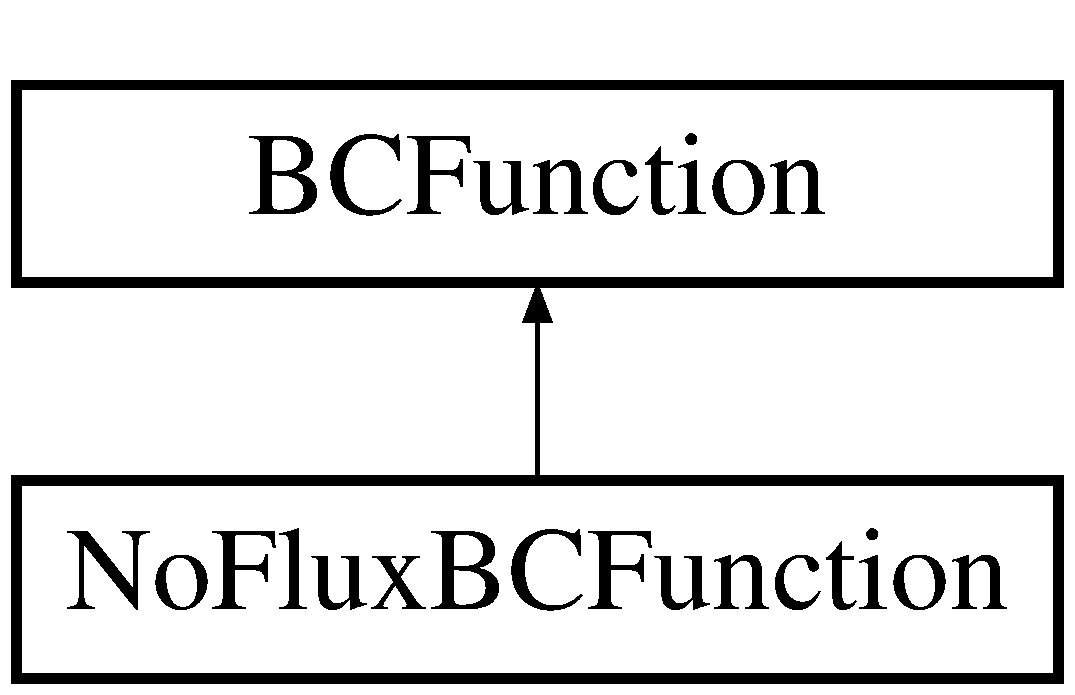
\includegraphics[height=2.000000cm]{class_no_flux_b_c_function}
\end{center}
\end{figure}
\subsection*{Public Member Functions}
\begin{DoxyCompactItemize}
\item 
\hypertarget{class_no_flux_b_c_function_a6243d50e9672fb6869a40bdb1f335cf3}{\hyperlink{class_no_flux_b_c_function_a6243d50e9672fb6869a40bdb1f335cf3}{No\-Flux\-B\-C\-Function} ()}\label{class_no_flux_b_c_function_a6243d50e9672fb6869a40bdb1f335cf3}

\begin{DoxyCompactList}\small\item\em Default constructor. \end{DoxyCompactList}\item 
\hypertarget{class_no_flux_b_c_function_a966de8831cfb254ff72d255f060c3d43}{\hyperlink{class_no_flux_b_c_function_a966de8831cfb254ff72d255f060c3d43}{No\-Flux\-B\-C\-Function} (bool a\-\_\-is\-Defined, \hyperlink{class_mushy_layer_params}{Mushy\-Layer\-Params} a\-\_\-params)}\label{class_no_flux_b_c_function_a966de8831cfb254ff72d255f060c3d43}

\begin{DoxyCompactList}\small\item\em Full constructor. \end{DoxyCompactList}\item 
\hypertarget{class_no_flux_b_c_function_a2ba95ac273b5afafd28a156fea4ae980}{virtual void \hyperlink{class_no_flux_b_c_function_a2ba95ac273b5afafd28a156fea4ae980}{operator()} (F\-Array\-Box \&a\-\_\-state, const Box \&a\-\_\-valid, const Problem\-Domain \&a\-\_\-domain, Real a\-\_\-dx, bool a\-\_\-homogeneous)}\label{class_no_flux_b_c_function_a2ba95ac273b5afafd28a156fea4ae980}

\begin{DoxyCompactList}\small\item\em Apply B\-C. \end{DoxyCompactList}\end{DoxyCompactItemize}
\subsection*{Public Attributes}
\begin{DoxyCompactItemize}
\item 
\hypertarget{class_no_flux_b_c_function_abcfc09a4099e8a362e2b2106d894fee5}{bool \hyperlink{class_no_flux_b_c_function_abcfc09a4099e8a362e2b2106d894fee5}{m\-\_\-is\-Defined}}\label{class_no_flux_b_c_function_abcfc09a4099e8a362e2b2106d894fee5}

\begin{DoxyCompactList}\small\item\em Is object defined? \end{DoxyCompactList}\item 
\hypertarget{class_no_flux_b_c_function_a2248e0ef0368d0a188a6baf8d7dd4682}{\hyperlink{class_mushy_layer_params}{Mushy\-Layer\-Params} \hyperlink{class_no_flux_b_c_function_a2248e0ef0368d0a188a6baf8d7dd4682}{m\-\_\-params}}\label{class_no_flux_b_c_function_a2248e0ef0368d0a188a6baf8d7dd4682}

\begin{DoxyCompactList}\small\item\em Physical parameters for the problem. \end{DoxyCompactList}\end{DoxyCompactItemize}


\subsection{Detailed Description}
Boundary condition for reflux correction. 

Sets correction = 0 on all boundaries 

The documentation for this class was generated from the following file\-:\begin{DoxyCompactItemize}
\item 
/home/parkinsonjl/mushy-\/layer/\-B\-Cutil/Phys\-B\-C\-Util.\-cpp\end{DoxyCompactItemize}

\hypertarget{class_phys_b_c_util}{\section{Phys\-B\-C\-Util Class Reference}
\label{class_phys_b_c_util}\index{Phys\-B\-C\-Util@{Phys\-B\-C\-Util}}
}


Big class to encapsulate physical boundary conditions.  




{\ttfamily \#include $<$Phys\-B\-C\-Util.\-H$>$}

\subsection*{Public Types}
\begin{DoxyCompactItemize}
\item 
enum \hyperlink{class_phys_b_c_util_a1aaacd3006840779878dc6287355a358}{Vel\-B\-C\-Type} \{ \\*
{\bfseries bogus\-B\-C} = -\/1, 
{\bfseries Solid\-Wall}, 
{\bfseries Inflow}, 
{\bfseries Outflow}, 
\\*
{\bfseries Outflow\-Normal}, 
{\bfseries Vel\-Inflow\-Outflow}, 
{\bfseries no\-Shear}, 
{\bfseries Symmetry}, 
\\*
{\bfseries Vel\-Inflow\-Plume}, 
{\bfseries N\-U\-M\-\_\-\-P\-H\-Y\-S\-\_\-\-B\-C\-\_\-\-T\-Y\-P\-E\-S}
 \}
\begin{DoxyCompactList}\small\item\em Different types of velocity boundary conditions. \end{DoxyCompactList}\item 
enum \hyperlink{class_phys_b_c_util_a1beb9821cf9e783e3742b82b7070c97a}{scalar\-B\-C\-Type} \{ \hyperlink{class_phys_b_c_util_a1beb9821cf9e783e3742b82b7070c97aa3c458c6b8958fb7d8f8f575725a0e91c}{Dirichlet}, 
\hyperlink{class_phys_b_c_util_a1beb9821cf9e783e3742b82b7070c97aae1ec2629a88cd0c687f102296e995d6b}{Neumann}, 
\hyperlink{class_phys_b_c_util_a1beb9821cf9e783e3742b82b7070c97aae85fc8bb407faa51331a6602f82577b7}{Inflow\-Outflow}, 
\hyperlink{class_phys_b_c_util_a1beb9821cf9e783e3742b82b7070c97aa3f9f8b4486f10b1ae3cef04b812d882f}{Only\-Inflow}
 \}
\begin{DoxyCompactList}\small\item\em Different options for scalar boundary conditions. \end{DoxyCompactList}\end{DoxyCompactItemize}
\subsection*{Public Member Functions}
\begin{DoxyCompactItemize}
\item 
\hyperlink{class_phys_b_c_util_a08574a3a8d645947c3914ef6eb56694f}{Phys\-B\-C\-Util} (\hyperlink{class_mushy_layer_params}{Mushy\-Layer\-Params} a\-\_\-params, Real a\-\_\-dx)
\item 
\hypertarget{class_phys_b_c_util_a499c4b2427896f35a2b4c4b857d17b89}{virtual \hyperlink{class_phys_b_c_util}{Phys\-B\-C\-Util} $\ast$ \hyperlink{class_phys_b_c_util_a499c4b2427896f35a2b4c4b857d17b89}{new\-Phys\-B\-C\-Util} () const }\label{class_phys_b_c_util_a499c4b2427896f35a2b4c4b857d17b89}

\begin{DoxyCompactList}\small\item\em \char`\"{}virtual\char`\"{} constructor \end{DoxyCompactList}\item 
virtual Tuple$<$ B\-C\-Holder, Space\-Dim $>$ \hyperlink{class_phys_b_c_util_ad86270197f828321cffe7c8f2b9d9110}{tracing\-Vel\-Func\-B\-C} () const 
\begin{DoxyCompactList}\small\item\em returns velocity B\-C for tracing (inviscid) \end{DoxyCompactList}\item 
virtual Tuple$<$ B\-C\-Holder, Space\-Dim $>$ \hyperlink{class_phys_b_c_util_a5702e30d8bc08c378544213430cabf4c}{advection\-Vel\-Func\-B\-C} (bool a\-\_\-is\-Viscous) const 
\begin{DoxyCompactList}\small\item\em added by petermc, 20 nov 2007 \end{DoxyCompactList}\item 
\hypertarget{class_phys_b_c_util_a525b2443f35d2fc7574cb13782d7cc67}{virtual Tuple$<$ B\-C\-Holder, Space\-Dim $>$ \hyperlink{class_phys_b_c_util_a525b2443f35d2fc7574cb13782d7cc67}{flux\-Extrap\-B\-C} () const }\label{class_phys_b_c_util_a525b2443f35d2fc7574cb13782d7cc67}

\begin{DoxyCompactList}\small\item\em Currently unused. \end{DoxyCompactList}\item 
\hypertarget{class_phys_b_c_util_abb7e75548708a66c6ac30b64d2461ab3}{virtual Tuple$<$ B\-C\-Holder, Space\-Dim $>$ \hyperlink{class_phys_b_c_util_abb7e75548708a66c6ac30b64d2461ab3}{u\-Star\-Func\-B\-C} (bool a\-\_\-is\-Viscous=false) const }\label{class_phys_b_c_util_abb7e75548708a66c6ac30b64d2461ab3}

\begin{DoxyCompactList}\small\item\em B\-C holder for $ \mathbf{u}^* $. \end{DoxyCompactList}\item 
\hypertarget{class_phys_b_c_util_a2925ca7d7b6a788bd84a8d4316000194}{virtual Tuple$<$ B\-C\-Holder, Space\-Dim $>$ \hyperlink{class_phys_b_c_util_a2925ca7d7b6a788bd84a8d4316000194}{edge\-Vel\-Func\-B\-C} (bool a\-\_\-is\-Viscous=false) const }\label{class_phys_b_c_util_a2925ca7d7b6a788bd84a8d4316000194}

\begin{DoxyCompactList}\small\item\em B\-C holder for $ \mathbf{u} $ (edge centred) \end{DoxyCompactList}\item 
\hypertarget{class_phys_b_c_util_a18a9e464ba4ebbc126de38b7678c87dc}{virtual Tuple$<$ B\-C\-Holder, Space\-Dim $>$ \hyperlink{class_phys_b_c_util_a18a9e464ba4ebbc126de38b7678c87dc}{porosity\-Face\-B\-C} () const }\label{class_phys_b_c_util_a18a9e464ba4ebbc126de38b7678c87dc}

\begin{DoxyCompactList}\small\item\em B\-C holder for porosity $ \chi $, (edge centred) \end{DoxyCompactList}\item 
\hypertarget{class_phys_b_c_util_a7bbf17a8fb9f268c1315cd663b69b9b7}{virtual Tuple$<$ B\-C\-Holder, Space\-Dim $>$ {\bfseries permeability\-Face\-B\-C} () const }\label{class_phys_b_c_util_a7bbf17a8fb9f268c1315cd663b69b9b7}

\item 
\hypertarget{class_phys_b_c_util_a247e8d8fe685f3a9ef56884d08c82fb9}{virtual Tuple$<$ B\-C\-Holder, Space\-Dim $>$ \hyperlink{class_phys_b_c_util_a247e8d8fe685f3a9ef56884d08c82fb9}{vel\-Extrap\-B\-C} (bool a\-\_\-is\-Viscous=false, int num\-\_\-ghost=1) const }\label{class_phys_b_c_util_a247e8d8fe685f3a9ef56884d08c82fb9}

\begin{DoxyCompactList}\small\item\em B\-C holder for velocity $ \mathbf{u} $ -\/ extrapolation. \end{DoxyCompactList}\item 
virtual B\-C\-Holder \hyperlink{class_phys_b_c_util_aac70ea0fdeca92be7adaef6317a52fe0}{viscous\-Reflux\-B\-C} (int a\-\_\-dir, bool a\-\_\-is\-Viscous=false) const 
\begin{DoxyCompactList}\small\item\em Fills interior ghost cells of vector field by extrapolation. \end{DoxyCompactList}\item 
virtual Phys\-I\-B\-C $\ast$ \hyperlink{class_phys_b_c_util_af5990ab84f0758727c35c27b4a02f35b}{advection\-Vel\-I\-B\-C} () const 
\begin{DoxyCompactList}\small\item\em returns a B\-C object compatible with A\-M\-R\-Godunov advection infrastructure \end{DoxyCompactList}\item 
\hypertarget{class_phys_b_c_util_afbc82bf7d509c99722005bbb202bd71e}{bool \hyperlink{class_phys_b_c_util_afbc82bf7d509c99722005bbb202bd71e}{is\-Defined} ()}\label{class_phys_b_c_util_afbc82bf7d509c99722005bbb202bd71e}

\begin{DoxyCompactList}\small\item\em Is object defined? \end{DoxyCompactList}\item 
\hypertarget{class_phys_b_c_util_a35dc4c0a9f1f3a7515c924d2de3dcaf7}{void \hyperlink{class_phys_b_c_util_a35dc4c0a9f1f3a7515c924d2de3dcaf7}{Dx} (const Real a\-\_\-dx)}\label{class_phys_b_c_util_a35dc4c0a9f1f3a7515c924d2de3dcaf7}

\begin{DoxyCompactList}\small\item\em sets cell spacing \end{DoxyCompactList}\item 
\hypertarget{class_phys_b_c_util_a58e8554dff0205baa224603fe7dfdc0a}{void {\bfseries convert\-B\-C\-Type} (const int a\-\_\-implicit\-B\-C, const Real a\-\_\-implicit\-Val, int \&a\-\_\-explicit\-B\-C, Real \&a\-\_\-explicit\-Val) const }\label{class_phys_b_c_util_a58e8554dff0205baa224603fe7dfdc0a}

\item 
\hypertarget{class_phys_b_c_util_acda802116f691baba67995132d60752b}{int {\bfseries convert\-B\-C\-Type} (const int a\-\_\-implicit\-B\-C) const }\label{class_phys_b_c_util_acda802116f691baba67995132d60752b}

\item 
\hypertarget{class_phys_b_c_util_a29d26fc7ceda182a4854307f6f8d62ae}{Real \hyperlink{class_phys_b_c_util_a29d26fc7ceda182a4854307f6f8d62ae}{Dx} () const }\label{class_phys_b_c_util_a29d26fc7ceda182a4854307f6f8d62ae}

\begin{DoxyCompactList}\small\item\em returns cell spacing \end{DoxyCompactList}\item 
\hypertarget{class_phys_b_c_util_ab0e771887c439318b0501b9f67a1b8c2}{void \hyperlink{class_phys_b_c_util_ab0e771887c439318b0501b9f67a1b8c2}{Time} (const Real a\-\_\-time)}\label{class_phys_b_c_util_ab0e771887c439318b0501b9f67a1b8c2}

\begin{DoxyCompactList}\small\item\em sets time \end{DoxyCompactList}\item 
\hypertarget{class_phys_b_c_util_a1b2bda9dea48021098134c846f487c6d}{Real \hyperlink{class_phys_b_c_util_a1b2bda9dea48021098134c846f487c6d}{Time} () const }\label{class_phys_b_c_util_a1b2bda9dea48021098134c846f487c6d}

\begin{DoxyCompactList}\small\item\em returns current time \end{DoxyCompactList}\item 
\hypertarget{class_phys_b_c_util_aacb13faac8c92afafe5ddc7d667e6181}{void \hyperlink{class_phys_b_c_util_aacb13faac8c92afafe5ddc7d667e6181}{set\-Adv\-Vel} (Level\-Data$<$ Flux\-Box $>$ $\ast$a\-\_\-adv\-Vel)}\label{class_phys_b_c_util_aacb13faac8c92afafe5ddc7d667e6181}

\begin{DoxyCompactList}\small\item\em Set pointer to advection velocity. \end{DoxyCompactList}\item 
\hypertarget{class_phys_b_c_util_ae121a247bdd5732a82af904ac77257e8}{Level\-Data$<$ Flux\-Box $>$ $\ast$ \hyperlink{class_phys_b_c_util_ae121a247bdd5732a82af904ac77257e8}{get\-Adv\-Vel} ()}\label{class_phys_b_c_util_ae121a247bdd5732a82af904ac77257e8}

\begin{DoxyCompactList}\small\item\em Get pointer to advection velocity. \end{DoxyCompactList}\item 
virtual B\-C\-Holder \hyperlink{class_phys_b_c_util_a62588222f0f6bf31efdab93760054077}{Level\-Pressure\-Func\-B\-C} () const 
\begin{DoxyCompactList}\small\item\em B\-C holder for pressure $ P $. \end{DoxyCompactList}\item 
virtual B\-C\-Holder \hyperlink{class_phys_b_c_util_a46b4a269ff7865055b6646575d11a600}{grad\-E\-Sync\-Func\-B\-C} () const 
\begin{DoxyCompactList}\small\item\em B\-C holder for synchronisation correction. \end{DoxyCompactList}\item 
\hypertarget{class_phys_b_c_util_a4d226e14d67824f313f3ff786c427c2d}{virtual B\-C\-Holder \hyperlink{class_phys_b_c_util_a4d226e14d67824f313f3ff786c427c2d}{grad\-Pi\-Func\-B\-C} () const }\label{class_phys_b_c_util_a4d226e14d67824f313f3ff786c427c2d}

\begin{DoxyCompactList}\small\item\em B\-C holder for $ \nabla \Pi $. \end{DoxyCompactList}\item 
\hypertarget{class_phys_b_c_util_a22628a8b9351997d1c753147765b7279}{virtual B\-C\-Holder \hyperlink{class_phys_b_c_util_a22628a8b9351997d1c753147765b7279}{extrap\-Func\-B\-C} () const }\label{class_phys_b_c_util_a22628a8b9351997d1c753147765b7279}

\begin{DoxyCompactList}\small\item\em Extrap B\-Cs on all domain boundaries. \end{DoxyCompactList}\item 
virtual B\-C\-Holder \hyperlink{class_phys_b_c_util_abee97d7d7bf3037aca0e1792a81a558d}{Freestream\-Corr\-Func\-B\-C} () const 
\begin{DoxyCompactList}\small\item\em B\-C holder for freestream correction. \end{DoxyCompactList}\item 
virtual B\-C\-Holder \hyperlink{class_phys_b_c_util_ab7b16d2dba8d3952a9a8321ecac5cb97}{Sync\-Proj\-Func\-B\-C} () const 
\begin{DoxyCompactList}\small\item\em B\-C holder for synchronisation projection. \end{DoxyCompactList}\item 
virtual B\-C\-Holder \hyperlink{class_phys_b_c_util_a19088e434b5c1510377761745e789d5f}{grad\-Mac\-Pressure\-Func\-B\-C} () const 
\begin{DoxyCompactList}\small\item\em B\-C holder for $ \nabla P $ in the M\-A\-C projection. \end{DoxyCompactList}\item 
virtual B\-C\-Holder \hyperlink{class_phys_b_c_util_a61e8e687697e7164f3e1a732a52fcbd5}{grad\-E\-Lambda\-Func\-B\-C} () const 
\begin{DoxyCompactList}\small\item\em B\-C holder for freestream preservation correction $ \nabla e_\lambda $. \end{DoxyCompactList}\item 
virtual B\-C\-Holder \hyperlink{class_phys_b_c_util_a91c00ce227d128cdd5cd996ad6142bec}{vel\-Func\-B\-C} (int a\-\_\-dir, bool a\-\_\-viscous, Interval interval=Interval(0, 0)) const 
\begin{DoxyCompactList}\small\item\em returns single-\/component B\-C for viscous solves \end{DoxyCompactList}\item 
virtual B\-C\-Holder \hyperlink{class_phys_b_c_util_a096c38e7c08e42f095456519d34bba4e}{extrapolation\-Func\-B\-C} (int a\-\_\-order=0) const 
\begin{DoxyCompactList}\small\item\em returns single-\/component B\-C \end{DoxyCompactList}\item 
virtual B\-C\-Holder \hyperlink{class_phys_b_c_util_a322ff42e655dd2a77b73e77f6b413159}{Basic\-Grad\-Pressure\-Func\-B\-C} () const 
\begin{DoxyCompactList}\small\item\em B\-C holder for $ \nabla P $. \end{DoxyCompactList}\item 
\hypertarget{class_phys_b_c_util_ad8f25c0af3d3b453a0d419cf0520349c}{virtual B\-C\-Holder {\bfseries stream\-Function\-B\-C} () const }\label{class_phys_b_c_util_ad8f25c0af3d3b453a0d419cf0520349c}

\item 
virtual B\-C\-Holder \hyperlink{class_phys_b_c_util_aadb095de5dc8347b10e0109c7754e764}{Basic\-Pressure\-Func\-B\-C} (bool a\-\_\-is\-Homogeneous) const 
\begin{DoxyCompactList}\small\item\em B\-C holder for pressure. \end{DoxyCompactList}\item 
\hypertarget{class_phys_b_c_util_aae91468f5b33eb3a2a52a3fc5af54d35}{virtual B\-C\-Holder \hyperlink{class_phys_b_c_util_aae91468f5b33eb3a2a52a3fc5af54d35}{Theta\-L\-Func\-B\-C} (bool a\-\_\-homogeneous=false, Level\-Data$<$ Flux\-Box $>$ $\ast$a\-\_\-adv\-Vel=N\-U\-L\-L) const }\label{class_phys_b_c_util_aae91468f5b33eb3a2a52a3fc5af54d35}

\begin{DoxyCompactList}\small\item\em B\-C holder for liquid concentration, $ \Theta_l $. \end{DoxyCompactList}\item 
\hypertarget{class_phys_b_c_util_ac73090123aca05c7b468f7d54cf85f92}{virtual B\-C\-Holder \hyperlink{class_phys_b_c_util_ac73090123aca05c7b468f7d54cf85f92}{Basictheta\-Func\-B\-C} (bool a\-\_\-homogeneous=false, Level\-Data$<$ Flux\-Box $>$ $\ast$a\-\_\-adv\-Vel=N\-U\-L\-L) const }\label{class_phys_b_c_util_ac73090123aca05c7b468f7d54cf85f92}

\begin{DoxyCompactList}\small\item\em B\-C holder for temperature, $ \theta $. \end{DoxyCompactList}\item 
\hypertarget{class_phys_b_c_util_a2508fcbc784f47bb77a38ed106a62fe2}{virtual B\-C\-Holder \hyperlink{class_phys_b_c_util_a2508fcbc784f47bb77a38ed106a62fe2}{Basic\-Porosity\-Func\-B\-C} (bool a\-\_\-homogeneous=false) const }\label{class_phys_b_c_util_a2508fcbc784f47bb77a38ed106a62fe2}

\begin{DoxyCompactList}\small\item\em B\-C holder for porosity, $ \chi $ (cell centred) \end{DoxyCompactList}\item 
\hypertarget{class_phys_b_c_util_a3d1deac59d469738b4cec7d61073510f}{virtual B\-C\-Holder \hyperlink{class_phys_b_c_util_a3d1deac59d469738b4cec7d61073510f}{Basic\-Porosity\-Face\-Func\-B\-C} (int a\-\_\-comp, bool a\-\_\-homogeneous=false) const }\label{class_phys_b_c_util_a3d1deac59d469738b4cec7d61073510f}

\begin{DoxyCompactList}\small\item\em B\-C holder for porosity, $ \chi $ (edge centred) \end{DoxyCompactList}\item 
\hypertarget{class_phys_b_c_util_a7af8441b5551c0105a88322d25659b1d}{virtual B\-C\-Holder \hyperlink{class_phys_b_c_util_a7af8441b5551c0105a88322d25659b1d}{Basic\-Permeability\-Func\-B\-C} (bool a\-\_\-homogeneous=false) const }\label{class_phys_b_c_util_a7af8441b5551c0105a88322d25659b1d}

\begin{DoxyCompactList}\small\item\em B\-C holder for permeability, $ \Pi $. \end{DoxyCompactList}\item 
\hypertarget{class_phys_b_c_util_ad78db7cfa2a4e13121c21eff7c52d8fe}{virtual B\-C\-Holder \hyperlink{class_phys_b_c_util_ad78db7cfa2a4e13121c21eff7c52d8fe}{Basic\-Permeability\-Face\-Func\-B\-C} (int a\-\_\-comp, bool a\-\_\-homogeneous=false) const }\label{class_phys_b_c_util_ad78db7cfa2a4e13121c21eff7c52d8fe}

\begin{DoxyCompactList}\small\item\em B\-C holder for permeability, $ \Pi $ (edge centred) \end{DoxyCompactList}\item 
\hypertarget{class_phys_b_c_util_a2e644dedf1a1af8ca706934373243b71}{virtual B\-C\-Holder \hyperlink{class_phys_b_c_util_a2e644dedf1a1af8ca706934373243b71}{Basic\-Enthalpy\-Func\-B\-C} (bool a\-\_\-homogeneous=false, Level\-Data$<$ Flux\-Box $>$ $\ast$a\-\_\-adv\-Vel=N\-U\-L\-L) const }\label{class_phys_b_c_util_a2e644dedf1a1af8ca706934373243b71}

\begin{DoxyCompactList}\small\item\em B\-C holder for enthalpy. \end{DoxyCompactList}\item 
\hypertarget{class_phys_b_c_util_a176ee6a7c294b39ccf125396a9b8ae83}{virtual B\-C\-Holder {\bfseries Basic\-Liquidus\-B\-C} (bool a\-\_\-homogeneous=false, Level\-Data$<$ Flux\-Box $>$ $\ast$a\-\_\-adv\-Vel=N\-U\-L\-L) const }\label{class_phys_b_c_util_a176ee6a7c294b39ccf125396a9b8ae83}

\item 
\hypertarget{class_phys_b_c_util_a4521d04f7b741128bfe22ecf7a619ae7}{virtual B\-C\-Holder {\bfseries Basic\-Eutectic\-B\-C} (bool a\-\_\-homogeneous=false, Level\-Data$<$ Flux\-Box $>$ $\ast$a\-\_\-adv\-Vel=N\-U\-L\-L) const }\label{class_phys_b_c_util_a4521d04f7b741128bfe22ecf7a619ae7}

\item 
\hypertarget{class_phys_b_c_util_a740da087df9ecb41abf9cab67a58a066}{virtual B\-C\-Holder {\bfseries Basic\-Solidus\-B\-C} (bool a\-\_\-homogeneous=false, Level\-Data$<$ Flux\-Box $>$ $\ast$a\-\_\-adv\-Vel=N\-U\-L\-L) const }\label{class_phys_b_c_util_a740da087df9ecb41abf9cab67a58a066}

\item 
\hypertarget{class_phys_b_c_util_acc28f597e867ec180867c8b6a4ebb07f}{virtual B\-C\-Holder \hyperlink{class_phys_b_c_util_acc28f597e867ec180867c8b6a4ebb07f}{Basic\-Scalar\-Func\-B\-C} (Real a\-\_\-top\-Val, Real a\-\_\-bottom\-Val, Real a\-\_\-plume\-Val, bool a\-\_\-homogeneous=false) const }\label{class_phys_b_c_util_acc28f597e867ec180867c8b6a4ebb07f}

\begin{DoxyCompactList}\small\item\em B\-C holder for some generic scalar. \end{DoxyCompactList}\item 
\hypertarget{class_phys_b_c_util_af438215be0fa9dc036688e366ac3838d}{virtual B\-C\-Holder \hyperlink{class_phys_b_c_util_af438215be0fa9dc036688e366ac3838d}{Theta\-Func\-B\-C} (bool a\-\_\-homogeneous=false, Level\-Data$<$ Flux\-Box $>$ $\ast$a\-\_\-adv\-Vel=N\-U\-L\-L) const }\label{class_phys_b_c_util_af438215be0fa9dc036688e366ac3838d}

\begin{DoxyCompactList}\small\item\em B\-C holder for bulk concentration $ \Theta $. \end{DoxyCompactList}\item 
\hypertarget{class_phys_b_c_util_a6410e91f537da1e28cc82c53c7cbdde4}{virtual B\-C\-Holder \hyperlink{class_phys_b_c_util_a6410e91f537da1e28cc82c53c7cbdde4}{basic\-Lambda\-Func\-B\-C} (bool a\-\_\-homogeneous=false, bool a\-\_\-scale\-With\-Porosity=false) const }\label{class_phys_b_c_util_a6410e91f537da1e28cc82c53c7cbdde4}

\begin{DoxyCompactList}\small\item\em B\-C holder for $ \lambda $ (for finding freestream preservation errors) \end{DoxyCompactList}\item 
\hypertarget{class_phys_b_c_util_a5959fe1d9dfdb154fea3b6c1f6fba434}{virtual B\-C\-Holder {\bfseries no\-Flux\-B\-C} () const }\label{class_phys_b_c_util_a5959fe1d9dfdb154fea3b6c1f6fba434}

\item 
virtual Phys\-I\-B\-C $\ast$ \hyperlink{class_phys_b_c_util_a3f43d8133f5a67f061a44e678018e6ae}{scalar\-Trace\-I\-B\-C} (Real\-Vect bc\-Val\-Lo, Real\-Vect bc\-Val\-Hi, Int\-Vect bc\-Type\-Lo, Int\-Vect bc\-Type\-Hi, Real a\-\_\-bc\-Plume\-Val=0.\-0, Vector$<$ Real $>$ a\-\_\-plume\-Bounds=Vector$<$ Real $>$(0)) const 
\begin{DoxyCompactList}\small\item\em Initial and Boundary Conditions for advecting scalars. \end{DoxyCompactList}\item 
\hypertarget{class_phys_b_c_util_a54d969da4cfdb8d222b8f688d26e2224}{virtual Phys\-I\-B\-C $\ast$ \hyperlink{class_phys_b_c_util_a54d969da4cfdb8d222b8f688d26e2224}{scalar\-Trace\-H\-C\-\_\-\-I\-B\-C} () const }\label{class_phys_b_c_util_a54d969da4cfdb8d222b8f688d26e2224}

\begin{DoxyCompactList}\small\item\em For multi component enthalpy-\/salinity solve. \end{DoxyCompactList}\item 
\hypertarget{class_phys_b_c_util_a63c20ba58745ef4b0ffddaeea56be2cb}{virtual Phys\-I\-B\-C $\ast$ {\bfseries scalar\-Trace\-H\-\_\-\-I\-B\-C} () const }\label{class_phys_b_c_util_a63c20ba58745ef4b0ffddaeea56be2cb}

\item 
\hypertarget{class_phys_b_c_util_a8010bc6fbfa7c558e0895289f3961c2d}{virtual Phys\-I\-B\-C $\ast$ {\bfseries scalar\-Trace\-C\-\_\-\-I\-B\-C} () const }\label{class_phys_b_c_util_a8010bc6fbfa7c558e0895289f3961c2d}

\item 
\hypertarget{class_phys_b_c_util_abe4ed912c0b312b1643dd16ea9af37fb}{virtual Phys\-I\-B\-C $\ast$ {\bfseries scalar\-Trace\-\_\-\-I\-B\-C} (Vector$<$ int $>$ a\-\_\-bc\-Type\-Hi, Vector$<$ int $>$ a\-\_\-bc\-Type\-Lo, Real\-Vect a\-\_\-bc\-Val\-Hi, Real\-Vect a\-\_\-bc\-Val\-Lo, Real a\-\_\-plume\-Inflow) const }\label{class_phys_b_c_util_abe4ed912c0b312b1643dd16ea9af37fb}

\item 
\hypertarget{class_phys_b_c_util_ae46dac1d9673a30a68be15fb27f4208c}{void {\bfseries apply\-Frame\-Advection\-B\-C} (Int\-Vect \&bc\-Type\-Hi, Int\-Vect \&bc\-Type\-Lo) const }\label{class_phys_b_c_util_ae46dac1d9673a30a68be15fb27f4208c}

\item 
\hypertarget{class_phys_b_c_util_a16ee868eeecae5c95db606a2bce0c181}{virtual Phys\-I\-B\-C $\ast$ \hyperlink{class_phys_b_c_util_a16ee868eeecae5c95db606a2bce0c181}{scalar\-Trace\-T\-Sl\-\_\-\-I\-B\-C} () const }\label{class_phys_b_c_util_a16ee868eeecae5c95db606a2bce0c181}

\begin{DoxyCompactList}\small\item\em For multi component enthalpy-\/salinity solve. \end{DoxyCompactList}\item 
\hypertarget{class_phys_b_c_util_ac2d93df710bd85569c3e943f46db6803}{virtual B\-C\-Holder \hyperlink{class_phys_b_c_util_ac2d93df710bd85569c3e943f46db6803}{temperature\-Liquid\-Salinity\-B\-C} (bool a\-\_\-homogeneous=false) const }\label{class_phys_b_c_util_ac2d93df710bd85569c3e943f46db6803}

\begin{DoxyCompactList}\small\item\em B\-C for object with two components, temperature and liquid salinity. \end{DoxyCompactList}\item 
\hypertarget{class_phys_b_c_util_ab852d537da8e31d294949510ce547c48}{virtual B\-C\-Holder \hyperlink{class_phys_b_c_util_ab852d537da8e31d294949510ce547c48}{enthalpy\-Salinity\-B\-C} (bool a\-\_\-homogeneous=false) const }\label{class_phys_b_c_util_ab852d537da8e31d294949510ce547c48}

\begin{DoxyCompactList}\small\item\em B\-C for object with two components, enthalpy and bulk salinity. \end{DoxyCompactList}\end{DoxyCompactItemize}
\subsection*{Public Attributes}
\begin{DoxyCompactItemize}
\item 
\hypertarget{class_phys_b_c_util_a1007b24a131e788c97781df04ae9037e}{\hyperlink{class_mushy_layer_params}{Mushy\-Layer\-Params} \hyperlink{class_phys_b_c_util_a1007b24a131e788c97781df04ae9037e}{m\-\_\-params}}\label{class_phys_b_c_util_a1007b24a131e788c97781df04ae9037e}

\begin{DoxyCompactList}\small\item\em Physical parameters for the system. \end{DoxyCompactList}\end{DoxyCompactItemize}
\subsection*{Protected Member Functions}
\begin{DoxyCompactItemize}
\item 
\hypertarget{class_phys_b_c_util_ad36596132d256e449f3cee586f8db8c5}{virtual B\-C\-Holder \hyperlink{class_phys_b_c_util_ad36596132d256e449f3cee586f8db8c5}{basic\-E\-C\-Vel\-Func\-B\-C} (bool a\-\_\-is\-Homogeneous, bool a\-\_\-is\-Viscous, int a\-\_\-comp, const Interval \&a\-\_\-interval) const }\label{class_phys_b_c_util_ad36596132d256e449f3cee586f8db8c5}

\begin{DoxyCompactList}\small\item\em B\-C\-Holder for edge centred velocity. \end{DoxyCompactList}\item 
\hypertarget{class_phys_b_c_util_a5575a252b14709be10c556f65f8d98d6}{virtual B\-C\-Holder \hyperlink{class_phys_b_c_util_a5575a252b14709be10c556f65f8d98d6}{basic\-C\-C\-Vel\-Func\-B\-C} (bool a\-\_\-is\-Homogeneous, bool a\-\_\-is\-Viscous, int a\-\_\-vel\-Component, const Interval \&a\-\_\-interval) const }\label{class_phys_b_c_util_a5575a252b14709be10c556f65f8d98d6}

\begin{DoxyCompactList}\small\item\em returns a B\-C\-Holder for cell-\/centered velocity \end{DoxyCompactList}\item 
\hypertarget{class_phys_b_c_util_aa296d3c2bac46734f50b55de22b45548}{virtual B\-C\-Holder \hyperlink{class_phys_b_c_util_aa296d3c2bac46734f50b55de22b45548}{extrap\-Vel\-Func\-B\-C} (bool a\-\_\-is\-Homogeneous, bool a\-\_\-is\-Viscous, int a\-\_\-comp, const Interval \&a\-\_\-interval, int num\-\_\-ghost=1) const }\label{class_phys_b_c_util_aa296d3c2bac46734f50b55de22b45548}

\begin{DoxyCompactList}\small\item\em Apply extrapolation B\-Cs to velocity. \end{DoxyCompactList}\item 
\hypertarget{class_phys_b_c_util_a25fcb4a8892a70b42eca416dfa01be63}{virtual B\-C\-Holder \hyperlink{class_phys_b_c_util_a25fcb4a8892a70b42eca416dfa01be63}{extrap\-Vel\-Func\-Interior} (bool a\-\_\-is\-Homogeneous, int a\-\_\-comp, const Interval \&a\-\_\-interval, int n\-\_\-ghost) const }\label{class_phys_b_c_util_a25fcb4a8892a70b42eca416dfa01be63}

\begin{DoxyCompactList}\small\item\em Apply extrapolation B\-Cs to velocity (interior ghost cells) \end{DoxyCompactList}\item 
virtual void \hyperlink{class_phys_b_c_util_a5abe105b9a924f6401b78ab6a5b4b1ab}{set\-B\-Cs} ()
\begin{DoxyCompactList}\small\item\em returns a B\-C\-Holder for edge-\/centered velocity \end{DoxyCompactList}\end{DoxyCompactItemize}
\subsection*{Protected Attributes}
\begin{DoxyCompactItemize}
\item 
\hypertarget{class_phys_b_c_util_a4c1aae9e1f5a676c93e0cd3bd7100f0b}{Tuple$<$ int, Space\-Dim $>$ \hyperlink{class_phys_b_c_util_a4c1aae9e1f5a676c93e0cd3bd7100f0b}{m\-\_\-lo\-B\-C}}\label{class_phys_b_c_util_a4c1aae9e1f5a676c93e0cd3bd7100f0b}

\begin{DoxyCompactList}\small\item\em contains the enumerated values for the lo-\/end B\-C \end{DoxyCompactList}\item 
\hypertarget{class_phys_b_c_util_a3469ac43534392033eb7d99c2398947b}{Tuple$<$ int, Space\-Dim $>$ \hyperlink{class_phys_b_c_util_a3469ac43534392033eb7d99c2398947b}{m\-\_\-hi\-B\-C}}\label{class_phys_b_c_util_a3469ac43534392033eb7d99c2398947b}

\begin{DoxyCompactList}\small\item\em contains the enumerated values for the hi-\/end B\-C \end{DoxyCompactList}\end{DoxyCompactItemize}


\subsection{Detailed Description}
Big class to encapsulate physical boundary conditions. 

\subsection{Member Enumeration Documentation}
\hypertarget{class_phys_b_c_util_a1beb9821cf9e783e3742b82b7070c97a}{\index{Phys\-B\-C\-Util@{Phys\-B\-C\-Util}!scalar\-B\-C\-Type@{scalar\-B\-C\-Type}}
\index{scalar\-B\-C\-Type@{scalar\-B\-C\-Type}!PhysBCUtil@{Phys\-B\-C\-Util}}
\subsubsection[{scalar\-B\-C\-Type}]{\setlength{\rightskip}{0pt plus 5cm}enum {\bf Phys\-B\-C\-Util\-::scalar\-B\-C\-Type}}}\label{class_phys_b_c_util_a1beb9821cf9e783e3742b82b7070c97a}


Different options for scalar boundary conditions. 

\begin{Desc}
\item[Enumerator]\par
\begin{description}
\index{Dirichlet@{Dirichlet}!Phys\-B\-C\-Util@{Phys\-B\-C\-Util}}\index{Phys\-B\-C\-Util@{Phys\-B\-C\-Util}!Dirichlet@{Dirichlet}}\item[{\em 
\hypertarget{class_phys_b_c_util_a1beb9821cf9e783e3742b82b7070c97aa3c458c6b8958fb7d8f8f575725a0e91c}{Dirichlet}\label{class_phys_b_c_util_a1beb9821cf9e783e3742b82b7070c97aa3c458c6b8958fb7d8f8f575725a0e91c}
}]Fix value at boundary. \index{Neumann@{Neumann}!Phys\-B\-C\-Util@{Phys\-B\-C\-Util}}\index{Phys\-B\-C\-Util@{Phys\-B\-C\-Util}!Neumann@{Neumann}}\item[{\em 
\hypertarget{class_phys_b_c_util_a1beb9821cf9e783e3742b82b7070c97aae1ec2629a88cd0c687f102296e995d6b}{Neumann}\label{class_phys_b_c_util_a1beb9821cf9e783e3742b82b7070c97aae1ec2629a88cd0c687f102296e995d6b}
}]Fix gradient at boundary. \index{Inflow\-Outflow@{Inflow\-Outflow}!Phys\-B\-C\-Util@{Phys\-B\-C\-Util}}\index{Phys\-B\-C\-Util@{Phys\-B\-C\-Util}!Inflow\-Outflow@{Inflow\-Outflow}}\item[{\em 
\hypertarget{class_phys_b_c_util_a1beb9821cf9e783e3742b82b7070c97aae85fc8bb407faa51331a6602f82577b7}{Inflow\-Outflow}\label{class_phys_b_c_util_a1beb9821cf9e783e3742b82b7070c97aae85fc8bb407faa51331a6602f82577b7}
}]Separate conditions for inflow and outflow regions. Where there's inflow -\/ dirichlet, where there's outflow -\/ zero normal gradient \index{Only\-Inflow@{Only\-Inflow}!Phys\-B\-C\-Util@{Phys\-B\-C\-Util}}\index{Phys\-B\-C\-Util@{Phys\-B\-C\-Util}!Only\-Inflow@{Only\-Inflow}}\item[{\em 
\hypertarget{class_phys_b_c_util_a1beb9821cf9e783e3742b82b7070c97aa3f9f8b4486f10b1ae3cef04b812d882f}{Only\-Inflow}\label{class_phys_b_c_util_a1beb9821cf9e783e3742b82b7070c97aa3f9f8b4486f10b1ae3cef04b812d882f}
}]Allow inflow but no outflow. For e.\-g. a plume forced into the domain. Enforce dirichlet B\-Cs everywhere, but with a different value for inflow vs outflow regions \end{description}
\end{Desc}
\hypertarget{class_phys_b_c_util_a1aaacd3006840779878dc6287355a358}{\index{Phys\-B\-C\-Util@{Phys\-B\-C\-Util}!Vel\-B\-C\-Type@{Vel\-B\-C\-Type}}
\index{Vel\-B\-C\-Type@{Vel\-B\-C\-Type}!PhysBCUtil@{Phys\-B\-C\-Util}}
\subsubsection[{Vel\-B\-C\-Type}]{\setlength{\rightskip}{0pt plus 5cm}enum {\bf Phys\-B\-C\-Util\-::\-Vel\-B\-C\-Type}}}\label{class_phys_b_c_util_a1aaacd3006840779878dc6287355a358}


Different types of velocity boundary conditions. 

Solid\-Wall -\/ no normal flow, no transverse flow is viscous Inflow -\/ Outflow -\/ Outflow\-Normal -\/ normal component has zero gradient at boundary, transverse component = 0 Vel\-Inflow\-Outflow -\/ no\-Shear -\/ Symmetry -\/ 

\subsection{Constructor \& Destructor Documentation}
\hypertarget{class_phys_b_c_util_a08574a3a8d645947c3914ef6eb56694f}{\index{Phys\-B\-C\-Util@{Phys\-B\-C\-Util}!Phys\-B\-C\-Util@{Phys\-B\-C\-Util}}
\index{Phys\-B\-C\-Util@{Phys\-B\-C\-Util}!PhysBCUtil@{Phys\-B\-C\-Util}}
\subsubsection[{Phys\-B\-C\-Util}]{\setlength{\rightskip}{0pt plus 5cm}Phys\-B\-C\-Util\-::\-Phys\-B\-C\-Util (
\begin{DoxyParamCaption}
\item[{{\bf Mushy\-Layer\-Params}}]{a\-\_\-params, }
\item[{Real}]{a\-\_\-dx}
\end{DoxyParamCaption}
)}}\label{class_phys_b_c_util_a08574a3a8d645947c3914ef6eb56694f}
this will access the Parm\-Parse database using the phys\-B\-C prefix and use it to define the physical B\-C types (hi and lo) in each direction. The B\-C type \char`\"{}custom\char`\"{} will imply that the B\-C is a somewhat nonstandard one, but that the derived class will know what to do with it. 

\subsection{Member Function Documentation}
\hypertarget{class_phys_b_c_util_a5702e30d8bc08c378544213430cabf4c}{\index{Phys\-B\-C\-Util@{Phys\-B\-C\-Util}!advection\-Vel\-Func\-B\-C@{advection\-Vel\-Func\-B\-C}}
\index{advection\-Vel\-Func\-B\-C@{advection\-Vel\-Func\-B\-C}!PhysBCUtil@{Phys\-B\-C\-Util}}
\subsubsection[{advection\-Vel\-Func\-B\-C}]{\setlength{\rightskip}{0pt plus 5cm}Tuple$<$ B\-C\-Holder, Space\-Dim $>$ Phys\-B\-C\-Util\-::advection\-Vel\-Func\-B\-C (
\begin{DoxyParamCaption}
\item[{bool}]{a\-\_\-is\-Viscous}
\end{DoxyParamCaption}
) const\hspace{0.3cm}{\ttfamily [virtual]}}}\label{class_phys_b_c_util_a5702e30d8bc08c378544213430cabf4c}


added by petermc, 20 nov 2007 

returns edge-\/centered vel B\-C for edge-\/ctrd vel (single component) \hypertarget{class_phys_b_c_util_af5990ab84f0758727c35c27b4a02f35b}{\index{Phys\-B\-C\-Util@{Phys\-B\-C\-Util}!advection\-Vel\-I\-B\-C@{advection\-Vel\-I\-B\-C}}
\index{advection\-Vel\-I\-B\-C@{advection\-Vel\-I\-B\-C}!PhysBCUtil@{Phys\-B\-C\-Util}}
\subsubsection[{advection\-Vel\-I\-B\-C}]{\setlength{\rightskip}{0pt plus 5cm}Phys\-I\-B\-C $\ast$ Phys\-B\-C\-Util\-::advection\-Vel\-I\-B\-C (
\begin{DoxyParamCaption}
{}
\end{DoxyParamCaption}
) const\hspace{0.3cm}{\ttfamily [virtual]}}}\label{class_phys_b_c_util_af5990ab84f0758727c35c27b4a02f35b}


returns a B\-C object compatible with A\-M\-R\-Godunov advection infrastructure 

this is a B\-C object used in the Patch\-Godunov stuff \hypertarget{class_phys_b_c_util_a322ff42e655dd2a77b73e77f6b413159}{\index{Phys\-B\-C\-Util@{Phys\-B\-C\-Util}!Basic\-Grad\-Pressure\-Func\-B\-C@{Basic\-Grad\-Pressure\-Func\-B\-C}}
\index{Basic\-Grad\-Pressure\-Func\-B\-C@{Basic\-Grad\-Pressure\-Func\-B\-C}!PhysBCUtil@{Phys\-B\-C\-Util}}
\subsubsection[{Basic\-Grad\-Pressure\-Func\-B\-C}]{\setlength{\rightskip}{0pt plus 5cm}B\-C\-Holder Phys\-B\-C\-Util\-::\-Basic\-Grad\-Pressure\-Func\-B\-C (
\begin{DoxyParamCaption}
{}
\end{DoxyParamCaption}
) const\hspace{0.3cm}{\ttfamily [virtual]}}}\label{class_phys_b_c_util_a322ff42e655dd2a77b73e77f6b413159}


B\-C holder for $ \nabla P $. 

Extrapolation B\-Cs on all boundaries \hypertarget{class_phys_b_c_util_aadb095de5dc8347b10e0109c7754e764}{\index{Phys\-B\-C\-Util@{Phys\-B\-C\-Util}!Basic\-Pressure\-Func\-B\-C@{Basic\-Pressure\-Func\-B\-C}}
\index{Basic\-Pressure\-Func\-B\-C@{Basic\-Pressure\-Func\-B\-C}!PhysBCUtil@{Phys\-B\-C\-Util}}
\subsubsection[{Basic\-Pressure\-Func\-B\-C}]{\setlength{\rightskip}{0pt plus 5cm}B\-C\-Holder Phys\-B\-C\-Util\-::\-Basic\-Pressure\-Func\-B\-C (
\begin{DoxyParamCaption}
\item[{bool}]{a\-\_\-is\-Homogeneous}
\end{DoxyParamCaption}
) const\hspace{0.3cm}{\ttfamily [virtual]}}}\label{class_phys_b_c_util_aadb095de5dc8347b10e0109c7754e764}


B\-C holder for pressure. 

For subcycled code. \hypertarget{class_phys_b_c_util_a096c38e7c08e42f095456519d34bba4e}{\index{Phys\-B\-C\-Util@{Phys\-B\-C\-Util}!extrapolation\-Func\-B\-C@{extrapolation\-Func\-B\-C}}
\index{extrapolation\-Func\-B\-C@{extrapolation\-Func\-B\-C}!PhysBCUtil@{Phys\-B\-C\-Util}}
\subsubsection[{extrapolation\-Func\-B\-C}]{\setlength{\rightskip}{0pt plus 5cm}B\-C\-Holder Phys\-B\-C\-Util\-::extrapolation\-Func\-B\-C (
\begin{DoxyParamCaption}
\item[{int}]{a\-\_\-order = {\ttfamily 0}}
\end{DoxyParamCaption}
) const\hspace{0.3cm}{\ttfamily [virtual]}}}\label{class_phys_b_c_util_a096c38e7c08e42f095456519d34bba4e}


returns single-\/component B\-C 

Be very careful with this function -\/ it fills C\-F ghost cells.

Applies B\-Cs to component in the Interval(a\-\_\-dir, a\-\_\-dir)returns multi-\/component B\-C for applying to fields which have been calculated Not for use when computing fields -\/ use \hyperlink{class_phys_b_c_util_a91c00ce227d128cdd5cd996ad6142bec}{vel\-Func\-B\-C()} for solves. 0th order extrapolation, also fills interior ghost cells \hypertarget{class_phys_b_c_util_abee97d7d7bf3037aca0e1792a81a558d}{\index{Phys\-B\-C\-Util@{Phys\-B\-C\-Util}!Freestream\-Corr\-Func\-B\-C@{Freestream\-Corr\-Func\-B\-C}}
\index{Freestream\-Corr\-Func\-B\-C@{Freestream\-Corr\-Func\-B\-C}!PhysBCUtil@{Phys\-B\-C\-Util}}
\subsubsection[{Freestream\-Corr\-Func\-B\-C}]{\setlength{\rightskip}{0pt plus 5cm}B\-C\-Holder Phys\-B\-C\-Util\-::\-Freestream\-Corr\-Func\-B\-C (
\begin{DoxyParamCaption}
{}
\end{DoxyParamCaption}
) const\hspace{0.3cm}{\ttfamily [virtual]}}}\label{class_phys_b_c_util_abee97d7d7bf3037aca0e1792a81a558d}


B\-C holder for freestream correction. 

Normal gradient = 0 \hypertarget{class_phys_b_c_util_a61e8e687697e7164f3e1a732a52fcbd5}{\index{Phys\-B\-C\-Util@{Phys\-B\-C\-Util}!grad\-E\-Lambda\-Func\-B\-C@{grad\-E\-Lambda\-Func\-B\-C}}
\index{grad\-E\-Lambda\-Func\-B\-C@{grad\-E\-Lambda\-Func\-B\-C}!PhysBCUtil@{Phys\-B\-C\-Util}}
\subsubsection[{grad\-E\-Lambda\-Func\-B\-C}]{\setlength{\rightskip}{0pt plus 5cm}B\-C\-Holder Phys\-B\-C\-Util\-::grad\-E\-Lambda\-Func\-B\-C (
\begin{DoxyParamCaption}
{}
\end{DoxyParamCaption}
) const\hspace{0.3cm}{\ttfamily [virtual]}}}\label{class_phys_b_c_util_a61e8e687697e7164f3e1a732a52fcbd5}


B\-C holder for freestream preservation correction $ \nabla e_\lambda $. 

Same as for $ \nabla P $ in general \hypertarget{class_phys_b_c_util_a46b4a269ff7865055b6646575d11a600}{\index{Phys\-B\-C\-Util@{Phys\-B\-C\-Util}!grad\-E\-Sync\-Func\-B\-C@{grad\-E\-Sync\-Func\-B\-C}}
\index{grad\-E\-Sync\-Func\-B\-C@{grad\-E\-Sync\-Func\-B\-C}!PhysBCUtil@{Phys\-B\-C\-Util}}
\subsubsection[{grad\-E\-Sync\-Func\-B\-C}]{\setlength{\rightskip}{0pt plus 5cm}B\-C\-Holder Phys\-B\-C\-Util\-::grad\-E\-Sync\-Func\-B\-C (
\begin{DoxyParamCaption}
{}
\end{DoxyParamCaption}
) const\hspace{0.3cm}{\ttfamily [virtual]}}}\label{class_phys_b_c_util_a46b4a269ff7865055b6646575d11a600}


B\-C holder for synchronisation correction. 

Just use same B\-C as $ \nabla P $ \hypertarget{class_phys_b_c_util_a19088e434b5c1510377761745e789d5f}{\index{Phys\-B\-C\-Util@{Phys\-B\-C\-Util}!grad\-Mac\-Pressure\-Func\-B\-C@{grad\-Mac\-Pressure\-Func\-B\-C}}
\index{grad\-Mac\-Pressure\-Func\-B\-C@{grad\-Mac\-Pressure\-Func\-B\-C}!PhysBCUtil@{Phys\-B\-C\-Util}}
\subsubsection[{grad\-Mac\-Pressure\-Func\-B\-C}]{\setlength{\rightskip}{0pt plus 5cm}B\-C\-Holder Phys\-B\-C\-Util\-::grad\-Mac\-Pressure\-Func\-B\-C (
\begin{DoxyParamCaption}
{}
\end{DoxyParamCaption}
) const\hspace{0.3cm}{\ttfamily [virtual]}}}\label{class_phys_b_c_util_a19088e434b5c1510377761745e789d5f}


B\-C holder for $ \nabla P $ in the M\-A\-C projection. 

Same as for $ \nabla P $ in general \hypertarget{class_phys_b_c_util_a62588222f0f6bf31efdab93760054077}{\index{Phys\-B\-C\-Util@{Phys\-B\-C\-Util}!Level\-Pressure\-Func\-B\-C@{Level\-Pressure\-Func\-B\-C}}
\index{Level\-Pressure\-Func\-B\-C@{Level\-Pressure\-Func\-B\-C}!PhysBCUtil@{Phys\-B\-C\-Util}}
\subsubsection[{Level\-Pressure\-Func\-B\-C}]{\setlength{\rightskip}{0pt plus 5cm}B\-C\-Holder Phys\-B\-C\-Util\-::\-Level\-Pressure\-Func\-B\-C (
\begin{DoxyParamCaption}
{}
\end{DoxyParamCaption}
) const\hspace{0.3cm}{\ttfamily [virtual]}}}\label{class_phys_b_c_util_a62588222f0f6bf31efdab93760054077}


B\-C holder for pressure $ P $. 

For subcycled code. \hypertarget{class_phys_b_c_util_a3f43d8133f5a67f061a44e678018e6ae}{\index{Phys\-B\-C\-Util@{Phys\-B\-C\-Util}!scalar\-Trace\-I\-B\-C@{scalar\-Trace\-I\-B\-C}}
\index{scalar\-Trace\-I\-B\-C@{scalar\-Trace\-I\-B\-C}!PhysBCUtil@{Phys\-B\-C\-Util}}
\subsubsection[{scalar\-Trace\-I\-B\-C}]{\setlength{\rightskip}{0pt plus 5cm}Phys\-I\-B\-C $\ast$ Phys\-B\-C\-Util\-::scalar\-Trace\-I\-B\-C (
\begin{DoxyParamCaption}
\item[{Real\-Vect}]{bc\-Val\-Lo, }
\item[{Real\-Vect}]{bc\-Val\-Hi, }
\item[{Int\-Vect}]{bc\-Type\-Lo, }
\item[{Int\-Vect}]{bc\-Type\-Hi, }
\item[{Real}]{a\-\_\-bc\-Plume\-Val = {\ttfamily 0.0}, }
\item[{Vector$<$ Real $>$}]{a\-\_\-plume\-Bounds = {\ttfamily Vector$<$Real$>$(0)}}
\end{DoxyParamCaption}
) const\hspace{0.3cm}{\ttfamily [virtual]}}}\label{class_phys_b_c_util_a3f43d8133f5a67f061a44e678018e6ae}


Initial and Boundary Conditions for advecting scalars. 

this is a B\-C object used in the Patch\-Godunov stuff \hypertarget{class_phys_b_c_util_a5abe105b9a924f6401b78ab6a5b4b1ab}{\index{Phys\-B\-C\-Util@{Phys\-B\-C\-Util}!set\-B\-Cs@{set\-B\-Cs}}
\index{set\-B\-Cs@{set\-B\-Cs}!PhysBCUtil@{Phys\-B\-C\-Util}}
\subsubsection[{set\-B\-Cs}]{\setlength{\rightskip}{0pt plus 5cm}void Phys\-B\-C\-Util\-::set\-B\-Cs (
\begin{DoxyParamCaption}
{}
\end{DoxyParamCaption}
)\hspace{0.3cm}{\ttfamily [protected]}, {\ttfamily [virtual]}}}\label{class_phys_b_c_util_a5abe105b9a924f6401b78ab6a5b4b1ab}


returns a B\-C\-Holder for edge-\/centered velocity 

interact with Parm\-Parse to set physical B\-C types \hypertarget{class_phys_b_c_util_ab7b16d2dba8d3952a9a8321ecac5cb97}{\index{Phys\-B\-C\-Util@{Phys\-B\-C\-Util}!Sync\-Proj\-Func\-B\-C@{Sync\-Proj\-Func\-B\-C}}
\index{Sync\-Proj\-Func\-B\-C@{Sync\-Proj\-Func\-B\-C}!PhysBCUtil@{Phys\-B\-C\-Util}}
\subsubsection[{Sync\-Proj\-Func\-B\-C}]{\setlength{\rightskip}{0pt plus 5cm}B\-C\-Holder Phys\-B\-C\-Util\-::\-Sync\-Proj\-Func\-B\-C (
\begin{DoxyParamCaption}
{}
\end{DoxyParamCaption}
) const\hspace{0.3cm}{\ttfamily [virtual]}}}\label{class_phys_b_c_util_ab7b16d2dba8d3952a9a8321ecac5cb97}


B\-C holder for synchronisation projection. 

Same B\-Cs as for pressure \hypertarget{class_phys_b_c_util_ad86270197f828321cffe7c8f2b9d9110}{\index{Phys\-B\-C\-Util@{Phys\-B\-C\-Util}!tracing\-Vel\-Func\-B\-C@{tracing\-Vel\-Func\-B\-C}}
\index{tracing\-Vel\-Func\-B\-C@{tracing\-Vel\-Func\-B\-C}!PhysBCUtil@{Phys\-B\-C\-Util}}
\subsubsection[{tracing\-Vel\-Func\-B\-C}]{\setlength{\rightskip}{0pt plus 5cm}Tuple$<$ B\-C\-Holder, Space\-Dim $>$ Phys\-B\-C\-Util\-::tracing\-Vel\-Func\-B\-C (
\begin{DoxyParamCaption}
{}
\end{DoxyParamCaption}
) const\hspace{0.3cm}{\ttfamily [virtual]}}}\label{class_phys_b_c_util_ad86270197f828321cffe7c8f2b9d9110}


returns velocity B\-C for tracing (inviscid) 

returns pre-\/projection velocity B\-C returns velocity B\-C for viscous source \hypertarget{class_phys_b_c_util_a91c00ce227d128cdd5cd996ad6142bec}{\index{Phys\-B\-C\-Util@{Phys\-B\-C\-Util}!vel\-Func\-B\-C@{vel\-Func\-B\-C}}
\index{vel\-Func\-B\-C@{vel\-Func\-B\-C}!PhysBCUtil@{Phys\-B\-C\-Util}}
\subsubsection[{vel\-Func\-B\-C}]{\setlength{\rightskip}{0pt plus 5cm}B\-C\-Holder Phys\-B\-C\-Util\-::vel\-Func\-B\-C (
\begin{DoxyParamCaption}
\item[{int}]{a\-\_\-dir, }
\item[{bool}]{a\-\_\-viscous, }
\item[{Interval}]{interval = {\ttfamily Interval(0,0)}}
\end{DoxyParamCaption}
) const\hspace{0.3cm}{\ttfamily [virtual]}}}\label{class_phys_b_c_util_a91c00ce227d128cdd5cd996ad6142bec}


returns single-\/component B\-C for viscous solves 

Applies B\-Cs to the component in the Interval(0,0) \hypertarget{class_phys_b_c_util_aac70ea0fdeca92be7adaef6317a52fe0}{\index{Phys\-B\-C\-Util@{Phys\-B\-C\-Util}!viscous\-Reflux\-B\-C@{viscous\-Reflux\-B\-C}}
\index{viscous\-Reflux\-B\-C@{viscous\-Reflux\-B\-C}!PhysBCUtil@{Phys\-B\-C\-Util}}
\subsubsection[{viscous\-Reflux\-B\-C}]{\setlength{\rightskip}{0pt plus 5cm}B\-C\-Holder Phys\-B\-C\-Util\-::viscous\-Reflux\-B\-C (
\begin{DoxyParamCaption}
\item[{int}]{a\-\_\-dir, }
\item[{bool}]{a\-\_\-is\-Viscous = {\ttfamily false}}
\end{DoxyParamCaption}
) const\hspace{0.3cm}{\ttfamily [virtual]}}}\label{class_phys_b_c_util_aac70ea0fdeca92be7adaef6317a52fe0}


Fills interior ghost cells of vector field by extrapolation. 

returns single-\/component B\-C for viscous refluxing solves 

The documentation for this class was generated from the following files\-:\begin{DoxyCompactItemize}
\item 
/home/parkinsonjl/mushy-\/layer/\-B\-Cutil/Phys\-B\-C\-Util.\-H\item 
/home/parkinsonjl/mushy-\/layer/\-B\-Cutil/Phys\-B\-C\-Util.\-cpp\end{DoxyCompactItemize}

\hypertarget{class_pressure_inflow_value_function}{\section{Pressure\-Inflow\-Value\-Function Class Reference}
\label{class_pressure_inflow_value_function}\index{Pressure\-Inflow\-Value\-Function@{Pressure\-Inflow\-Value\-Function}}
}
Inheritance diagram for Pressure\-Inflow\-Value\-Function\-:\begin{figure}[H]
\begin{center}
\leavevmode
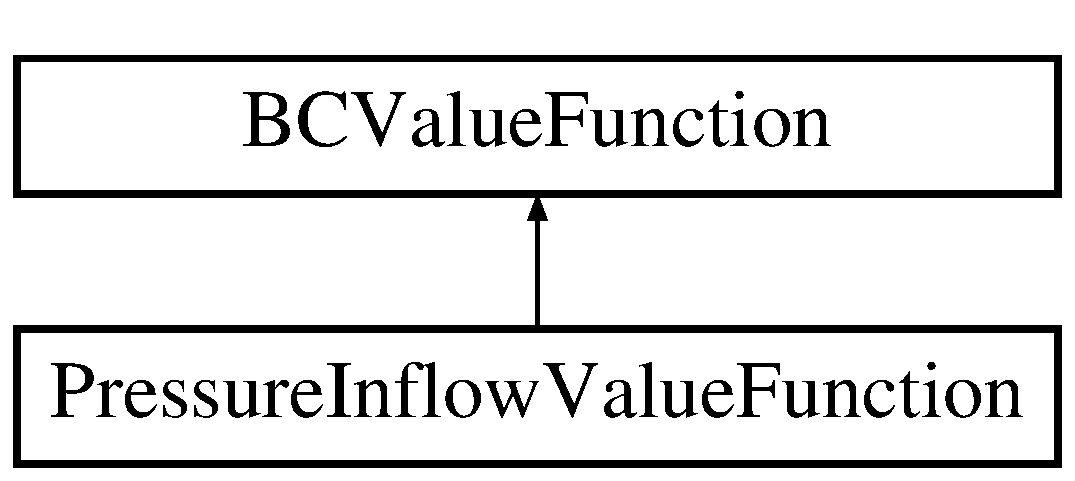
\includegraphics[height=2.000000cm]{class_pressure_inflow_value_function}
\end{center}
\end{figure}
\subsection*{Public Member Functions}
\begin{DoxyCompactItemize}
\item 
\hypertarget{class_pressure_inflow_value_function_aafa131789b607de20fefcca422d6795c}{\hyperlink{class_pressure_inflow_value_function_aafa131789b607de20fefcca422d6795c}{Pressure\-Inflow\-Value\-Function} ()}\label{class_pressure_inflow_value_function_aafa131789b607de20fefcca422d6795c}

\begin{DoxyCompactList}\small\item\em Default constructor. \end{DoxyCompactList}\item 
\hypertarget{class_pressure_inflow_value_function_a2907075ed6815d19bb140409dd79f5b5}{\hyperlink{class_pressure_inflow_value_function_a2907075ed6815d19bb140409dd79f5b5}{Pressure\-Inflow\-Value\-Function} (Real a\-\_\-value, int a\-\_\-n\-Comp, Real a\-\_\-inflow\-Value, Real a\-\_\-plume\-Start, Real a\-\_\-plume\-End, \hyperlink{class_mushy_layer_params}{Mushy\-Layer\-Params} $\ast$a\-\_\-params)}\label{class_pressure_inflow_value_function_a2907075ed6815d19bb140409dd79f5b5}

\begin{DoxyCompactList}\small\item\em Constructor. \end{DoxyCompactList}\item 
\hypertarget{class_pressure_inflow_value_function_ae700fea713b189f7b4ce066290f8b14e}{virtual void \hyperlink{class_pressure_inflow_value_function_ae700fea713b189f7b4ce066290f8b14e}{operator()} (Real $\ast$a\-\_\-pos, int $\ast$a\-\_\-dir, Side\-::\-Lo\-Hi\-Side $\ast$a\-\_\-side, Real $\ast$a\-\_\-value)}\label{class_pressure_inflow_value_function_ae700fea713b189f7b4ce066290f8b14e}

\begin{DoxyCompactList}\small\item\em Apply B\-C. \end{DoxyCompactList}\end{DoxyCompactItemize}
\subsection*{Public Attributes}
\begin{DoxyCompactItemize}
\item 
\hypertarget{class_pressure_inflow_value_function_a4ea988fb2567fad484acbdd1192f04c1}{Real \hyperlink{class_pressure_inflow_value_function_a4ea988fb2567fad484acbdd1192f04c1}{m\-\_\-value}}\label{class_pressure_inflow_value_function_a4ea988fb2567fad484acbdd1192f04c1}

\begin{DoxyCompactList}\small\item\em The constant value to apply. \end{DoxyCompactList}\item 
\hypertarget{class_pressure_inflow_value_function_a696bcf66ca28efa96314cb959dfb9f6a}{int \hyperlink{class_pressure_inflow_value_function_a696bcf66ca28efa96314cb959dfb9f6a}{m\-\_\-n\-Comp}}\label{class_pressure_inflow_value_function_a696bcf66ca28efa96314cb959dfb9f6a}

\begin{DoxyCompactList}\small\item\em The component to apply this B\-C to. \end{DoxyCompactList}\item 
\hypertarget{class_pressure_inflow_value_function_acb7b9ec6085a1b79ed4d7bf341185a32}{Real {\bfseries m\-\_\-inflow\-Value}}\label{class_pressure_inflow_value_function_acb7b9ec6085a1b79ed4d7bf341185a32}

\item 
\hypertarget{class_pressure_inflow_value_function_a14ffe6da33fc18c3394805b8934e9cfc}{Real {\bfseries m\-\_\-plume\-Start}}\label{class_pressure_inflow_value_function_a14ffe6da33fc18c3394805b8934e9cfc}

\item 
\hypertarget{class_pressure_inflow_value_function_ae342d40736d7519d777db87979f2b713}{Real {\bfseries m\-\_\-plume\-End}}\label{class_pressure_inflow_value_function_ae342d40736d7519d777db87979f2b713}

\item 
\hypertarget{class_pressure_inflow_value_function_a77a3ee87530c9cdc4b13a6373addb651}{\hyperlink{class_mushy_layer_params}{Mushy\-Layer\-Params} $\ast$ {\bfseries m\-\_\-params}}\label{class_pressure_inflow_value_function_a77a3ee87530c9cdc4b13a6373addb651}

\end{DoxyCompactItemize}


The documentation for this class was generated from the following file\-:\begin{DoxyCompactItemize}
\item 
/home/parkinsonjl/mushy-\/layer/\-B\-Cutil/Phys\-B\-C\-Util.\-cpp\end{DoxyCompactItemize}

\hypertarget{classspline}{\section{spline Class Reference}
\label{classspline}\index{spline@{spline}}
}
\subsection*{Public Types}
\begin{DoxyCompactItemize}
\item 
enum {\bfseries bd\-\_\-type} \{ {\bfseries first\-\_\-deriv} = 1, 
{\bfseries second\-\_\-deriv} = 2
 \}
\end{DoxyCompactItemize}
\subsection*{Public Member Functions}
\begin{DoxyCompactItemize}
\item 
\hypertarget{classspline_a8faa0e24c31c45b976606e1376e2eff2}{void {\bfseries set\-\_\-boundary} (bd\-\_\-type left, Real left\-\_\-value, bd\-\_\-type right, Real right\-\_\-value, bool force\-\_\-linear\-\_\-extrapolation=false)}\label{classspline_a8faa0e24c31c45b976606e1376e2eff2}

\item 
\hypertarget{classspline_abfb0f9a39a5c59e72aa59e0f1ce8cc6d}{void {\bfseries set\-\_\-points} (const std\-::vector$<$ Real $>$ \&x, const std\-::vector$<$ Real $>$ \&y, bool cubic\-\_\-spline=true)}\label{classspline_abfb0f9a39a5c59e72aa59e0f1ce8cc6d}

\item 
\hypertarget{classspline_a89cf037a96ee3d16af5f4d640e8e5b04}{Real {\bfseries operator()} (Real x) const }\label{classspline_a89cf037a96ee3d16af5f4d640e8e5b04}

\end{DoxyCompactItemize}


The documentation for this class was generated from the following files\-:\begin{DoxyCompactItemize}
\item 
/home/parkinsonjl/mushy-\/layer/src/Chombo\-Spline.\-h\item 
/home/parkinsonjl/mushy-\/layer/src/Chombo\-Spline.\-cpp\end{DoxyCompactItemize}

\hypertarget{class_stream_function_b_c}{\section{Stream\-Function\-B\-C Class Reference}
\label{class_stream_function_b_c}\index{Stream\-Function\-B\-C@{Stream\-Function\-B\-C}}
}


Boundary conditions for pressure $P$ (subcycled version)  


Inheritance diagram for Stream\-Function\-B\-C\-:\begin{figure}[H]
\begin{center}
\leavevmode
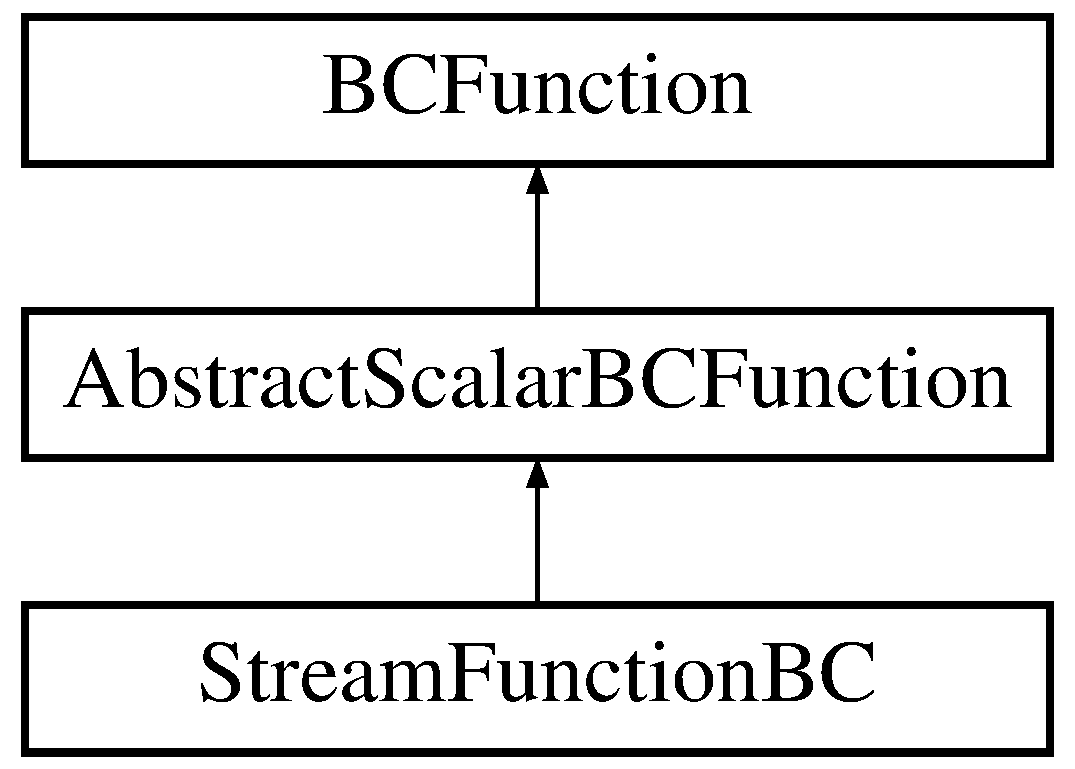
\includegraphics[height=3.000000cm]{class_stream_function_b_c}
\end{center}
\end{figure}
\subsection*{Public Member Functions}
\begin{DoxyCompactItemize}
\item 
\hypertarget{class_stream_function_b_c_a48da0de78c77018a8607988d836ffed0}{{\bfseries Stream\-Function\-B\-C} (bool a\-\_\-is\-Defined, \hyperlink{class_mushy_layer_params}{Mushy\-Layer\-Params} a\-\_\-params, bool a\-\_\-homogeneous, Level\-Data$<$ Flux\-Box $>$ $\ast$a\-\_\-adv\-Vel, Real a\-\_\-dx)}\label{class_stream_function_b_c_a48da0de78c77018a8607988d836ffed0}

\item 
\hypertarget{class_stream_function_b_c_ad87081663cc380e95de4fba24ddc4e39}{void \hyperlink{class_stream_function_b_c_ad87081663cc380e95de4fba24ddc4e39}{operator()} (F\-Array\-Box \&a\-\_\-state, const Box \&a\-\_\-valid, const Problem\-Domain \&a\-\_\-domain, Real a\-\_\-dx, bool a\-\_\-homogeneous)}\label{class_stream_function_b_c_ad87081663cc380e95de4fba24ddc4e39}

\begin{DoxyCompactList}\small\item\em Apply B\-C. \end{DoxyCompactList}\end{DoxyCompactItemize}
\subsection*{Additional Inherited Members}


\subsection{Detailed Description}
Boundary conditions for pressure $P$ (subcycled version) 

The documentation for this class was generated from the following file\-:\begin{DoxyCompactItemize}
\item 
/home/parkinsonjl/mushy-\/layer/\-B\-Cutil/Phys\-B\-C\-Util.\-cpp\end{DoxyCompactItemize}

\hypertarget{class_vel_b_c_holder}{\section{Vel\-B\-C\-Holder Class Reference}
\label{class_vel_b_c_holder}\index{Vel\-B\-C\-Holder@{Vel\-B\-C\-Holder}}
}


this is a physical B\-C class designed to handle velocities  




{\ttfamily \#include $<$Vel\-B\-C\-Holder.\-H$>$}

\subsection*{Public Member Functions}
\begin{DoxyCompactItemize}
\item 
\hypertarget{class_vel_b_c_holder_af5fa130e47bbac1e8f01ef5e4ff8453d}{\hyperlink{class_vel_b_c_holder_af5fa130e47bbac1e8f01ef5e4ff8453d}{Vel\-B\-C\-Holder} ()}\label{class_vel_b_c_holder_af5fa130e47bbac1e8f01ef5e4ff8453d}

\begin{DoxyCompactList}\small\item\em Default constructore. \end{DoxyCompactList}\item 
\hypertarget{class_vel_b_c_holder_a8946f96dbe531366cb223f87678e3110}{\hyperlink{class_vel_b_c_holder_a8946f96dbe531366cb223f87678e3110}{Vel\-B\-C\-Holder} (const Tuple$<$ B\-C\-Holder, Space\-Dim $>$ \&a\-\_\-component\-B\-C)}\label{class_vel_b_c_holder_a8946f96dbe531366cb223f87678e3110}

\begin{DoxyCompactList}\small\item\em Full constructore. \end{DoxyCompactList}\item 
\hypertarget{class_vel_b_c_holder_a3c80e1db72a619f73d535f441824ee82}{virtual \hyperlink{class_vel_b_c_holder_a3c80e1db72a619f73d535f441824ee82}{$\sim$\-Vel\-B\-C\-Holder} ()}\label{class_vel_b_c_holder_a3c80e1db72a619f73d535f441824ee82}

\begin{DoxyCompactList}\small\item\em Destructore. \end{DoxyCompactList}\item 
\hypertarget{class_vel_b_c_holder_a917796c7b5448f28fb4a15eae90e86a3}{virtual void \hyperlink{class_vel_b_c_holder_a917796c7b5448f28fb4a15eae90e86a3}{apply\-B\-Cs} (Level\-Data$<$ F\-Array\-Box $>$ \&a\-\_\-state, const Disjoint\-Box\-Layout \&a\-\_\-valid, const Problem\-Domain \&a\-\_\-domain, const Real a\-\_\-dx, bool a\-\_\-homogeneous)}\label{class_vel_b_c_holder_a917796c7b5448f28fb4a15eae90e86a3}

\begin{DoxyCompactList}\small\item\em Apply B\-Cs to a\-\_\-state. \end{DoxyCompactList}\end{DoxyCompactItemize}
\subsection*{Protected Attributes}
\begin{DoxyCompactItemize}
\item 
\hypertarget{class_vel_b_c_holder_a96bc0178395c31ab7ecc41538f63f457}{Tuple$<$ B\-C\-Holder, Space\-Dim $>$ \hyperlink{class_vel_b_c_holder_a96bc0178395c31ab7ecc41538f63f457}{m\-\_\-component\-B\-C}}\label{class_vel_b_c_holder_a96bc0178395c31ab7ecc41538f63f457}

\begin{DoxyCompactList}\small\item\em B\-C\-Holders for each component. \end{DoxyCompactList}\end{DoxyCompactItemize}


\subsection{Detailed Description}
this is a physical B\-C class designed to handle velocities 

this class is handles velocities, which are by their nature multicomponent 

The documentation for this class was generated from the following files\-:\begin{DoxyCompactItemize}
\item 
/home/parkinsonjl/mushy-\/layer/\-B\-Cutil/Vel\-B\-C\-Holder.\-H\item 
/home/parkinsonjl/mushy-\/layer/\-B\-Cutil/Vel\-B\-C\-Holder.\-cpp\end{DoxyCompactItemize}

\hypertarget{class_vel_i_b_c}{\section{Vel\-I\-B\-C Class Reference}
\label{class_vel_i_b_c}\index{Vel\-I\-B\-C@{Vel\-I\-B\-C}}
}


I\-B\-C for simple Velocity advection (solid wall) boundary conditions.  




{\ttfamily \#include $<$Vel\-I\-B\-C.\-H$>$}

Inheritance diagram for Vel\-I\-B\-C\-:\begin{figure}[H]
\begin{center}
\leavevmode
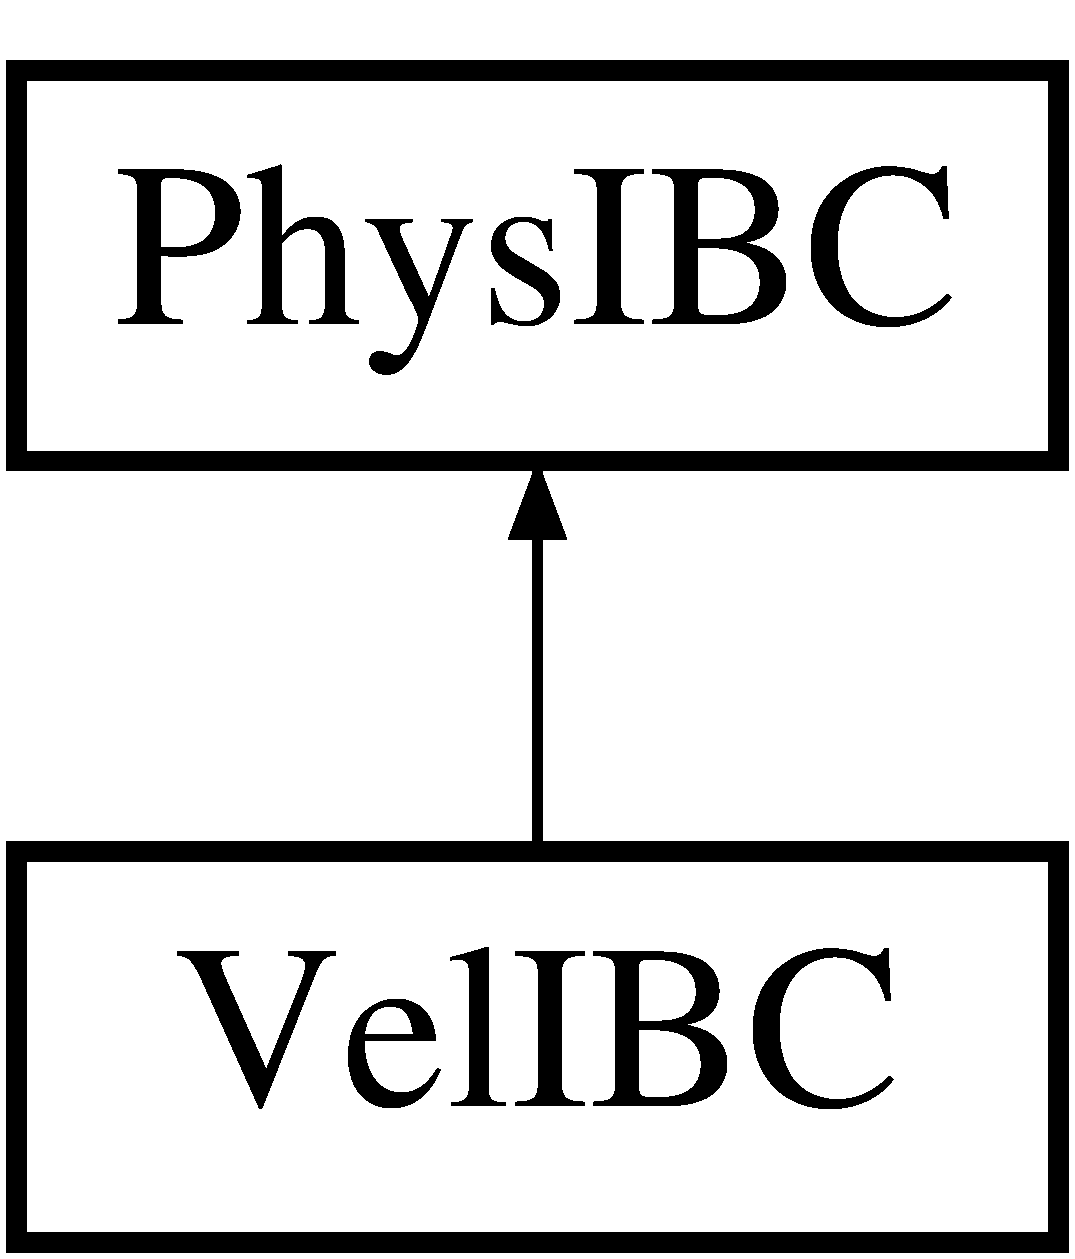
\includegraphics[height=2.000000cm]{class_vel_i_b_c}
\end{center}
\end{figure}
\subsection*{Public Member Functions}
\begin{DoxyCompactItemize}
\item 
\hypertarget{class_vel_i_b_c_a5823ec0d34fc039346f6f5970ac20393}{\hyperlink{class_vel_i_b_c_a5823ec0d34fc039346f6f5970ac20393}{Vel\-I\-B\-C} ()}\label{class_vel_i_b_c_a5823ec0d34fc039346f6f5970ac20393}

\begin{DoxyCompactList}\small\item\em Null constructor. \end{DoxyCompactList}\item 
\hypertarget{class_vel_i_b_c_a4b4e45d8bcd831ee73e360ca953fc3e3}{\hyperlink{class_vel_i_b_c_a4b4e45d8bcd831ee73e360ca953fc3e3}{$\sim$\-Vel\-I\-B\-C} ()}\label{class_vel_i_b_c_a4b4e45d8bcd831ee73e360ca953fc3e3}

\begin{DoxyCompactList}\small\item\em Destructor. \end{DoxyCompactList}\item 
Phys\-I\-B\-C $\ast$ \hyperlink{class_vel_i_b_c_ac53daf9706542e3fa4734c8701f5fff5}{new\-\_\-phys\-I\-B\-C} ()
\begin{DoxyCompactList}\small\item\em Factory method -\/ this object is its own factory. \end{DoxyCompactList}\item 
\hypertarget{class_vel_i_b_c_a67c793da1efebd887de7b0c7907b7e5b}{void \hyperlink{class_vel_i_b_c_a67c793da1efebd887de7b0c7907b7e5b}{set\-Default\-Values} ()}\label{class_vel_i_b_c_a67c793da1efebd887de7b0c7907b7e5b}

\begin{DoxyCompactList}\small\item\em set default boundary values \end{DoxyCompactList}\item 
\hypertarget{class_vel_i_b_c_a30d5d96e3f384b7fa82d919a424c7847}{void \hyperlink{class_vel_i_b_c_a30d5d96e3f384b7fa82d919a424c7847}{prim\-B\-C} (F\-Array\-Box \&a\-\_\-\-W\-Gdnv, const F\-Array\-Box \&a\-\_\-\-Wextrap, const F\-Array\-Box \&a\-\_\-\-W, const int \&a\-\_\-dir, const Side\-::\-Lo\-Hi\-Side \&a\-\_\-side, const Real \&a\-\_\-time)}\label{class_vel_i_b_c_a30d5d96e3f384b7fa82d919a424c7847}

\begin{DoxyCompactList}\small\item\em Set boundary fluxes. \end{DoxyCompactList}\item 
void \hyperlink{class_vel_i_b_c_a39ac3b18e885c749a1081ba7042941df}{set\-Bdry\-Slopes} (F\-Array\-Box \&a\-\_\-d\-W, const F\-Array\-Box \&a\-\_\-\-W, const int \&a\-\_\-dir, const Real \&a\-\_\-time)
\begin{DoxyCompactList}\small\item\em Set boundary slopes. \end{DoxyCompactList}\item 
void \hyperlink{class_vel_i_b_c_a0f2d126d3a569f828e0370c0c7dc6ec9}{initialize} (Level\-Data$<$ F\-Array\-Box $>$ \&a\-\_\-\-U)
\begin{DoxyCompactList}\small\item\em Set up initial conditions. \end{DoxyCompactList}\item 
\hypertarget{class_vel_i_b_c_a6b43f398d36e8aeb1ca17d11003b57f4}{void \hyperlink{class_vel_i_b_c_a6b43f398d36e8aeb1ca17d11003b57f4}{advection\-Vel} (const Real\-Vect \&a\-\_\-adv\-Vel)}\label{class_vel_i_b_c_a6b43f398d36e8aeb1ca17d11003b57f4}

\begin{DoxyCompactList}\small\item\em set velocity \end{DoxyCompactList}\item 
\hypertarget{class_vel_i_b_c_aa6ee7928a2f0d92c6420c4ac0e29b0e6}{const Real\-Vect \& \hyperlink{class_vel_i_b_c_aa6ee7928a2f0d92c6420c4ac0e29b0e6}{advection\-Vel} () const }\label{class_vel_i_b_c_aa6ee7928a2f0d92c6420c4ac0e29b0e6}

\begin{DoxyCompactList}\small\item\em Not sure why we have this. \end{DoxyCompactList}\item 
\hypertarget{class_vel_i_b_c_acbb613201240705e212ba21f906ba08e}{void \hyperlink{class_vel_i_b_c_acbb613201240705e212ba21f906ba08e}{prob\-Type} (const int a\-\_\-probtype)}\label{class_vel_i_b_c_acbb613201240705e212ba21f906ba08e}

\begin{DoxyCompactList}\small\item\em set problem type \end{DoxyCompactList}\item 
\hypertarget{class_vel_i_b_c_a5f45d506e02001c6c9b2034c973dc44e}{void \hyperlink{class_vel_i_b_c_a5f45d506e02001c6c9b2034c973dc44e}{set\-Normal\-Wall\-Vel} (Real a\-\_\-bc\-Val, int a\-\_\-dir, Side\-::\-Lo\-Hi\-Side a\-\_\-hi\-Lo)}\label{class_vel_i_b_c_a5f45d506e02001c6c9b2034c973dc44e}

\begin{DoxyCompactList}\small\item\em set boundary value (default is 0) \end{DoxyCompactList}\item 
\hypertarget{class_vel_i_b_c_a7336cd5660b2f29b9d59eacb3fa60ae5}{Real \hyperlink{class_vel_i_b_c_a7336cd5660b2f29b9d59eacb3fa60ae5}{get\-Normal\-Wall\-Vel} (int a\-\_\-dir, Side\-::\-Lo\-Hi\-Side a\-\_\-hi\-Lo) const }\label{class_vel_i_b_c_a7336cd5660b2f29b9d59eacb3fa60ae5}

\begin{DoxyCompactList}\small\item\em access boundary value \end{DoxyCompactList}\item 
\hypertarget{class_vel_i_b_c_a927055b4423e2ff7f412a36a7c7f8072}{void \hyperlink{class_vel_i_b_c_a927055b4423e2ff7f412a36a7c7f8072}{set\-Slope\-Value} (Real a\-\_\-slope\-Val, int a\-\_\-dir, Side\-::\-Lo\-Hi\-Side a\-\_\-hi\-Lo)}\label{class_vel_i_b_c_a927055b4423e2ff7f412a36a7c7f8072}

\begin{DoxyCompactList}\small\item\em set slope value (default is 0) \end{DoxyCompactList}\item 
\hypertarget{class_vel_i_b_c_af8d199f84cc3bfc4aae0c1c27a430dda}{Real \hyperlink{class_vel_i_b_c_af8d199f84cc3bfc4aae0c1c27a430dda}{get\-Slope\-Value} (int a\-\_\-dir, Side\-::\-Lo\-Hi\-Side a\-\_\-hi\-Lo) const }\label{class_vel_i_b_c_af8d199f84cc3bfc4aae0c1c27a430dda}

\begin{DoxyCompactList}\small\item\em access slope value \end{DoxyCompactList}\item 
\hypertarget{class_vel_i_b_c_a16760cd6971354c37ebe7e7482446ec4}{void \hyperlink{class_vel_i_b_c_a16760cd6971354c37ebe7e7482446ec4}{art\-Visc\-B\-C} (F\-Array\-Box \&a\-\_\-\-F, const F\-Array\-Box \&a\-\_\-\-U, const F\-Array\-Box \&a\-\_\-div\-Vel, const int \&a\-\_\-dir, const Real \&a\-\_\-time)}\label{class_vel_i_b_c_a16760cd6971354c37ebe7e7482446ec4}

\begin{DoxyCompactList}\small\item\em Apply artifical viscosity B\-C. \end{DoxyCompactList}\item 
\hypertarget{class_vel_i_b_c_a3133837da4e4555196362e6a7c73cd56}{int \hyperlink{class_vel_i_b_c_a3133837da4e4555196362e6a7c73cd56}{prob\-Type} () const }\label{class_vel_i_b_c_a3133837da4e4555196362e6a7c73cd56}

\begin{DoxyCompactList}\small\item\em accessor \end{DoxyCompactList}\end{DoxyCompactItemize}
\subsection*{Protected Attributes}
\begin{DoxyCompactItemize}
\item 
\hypertarget{class_vel_i_b_c_a3e9192d36c775a9b052578c5ec6a3afc}{Real\-Vect \hyperlink{class_vel_i_b_c_a3e9192d36c775a9b052578c5ec6a3afc}{m\-\_\-velocity}}\label{class_vel_i_b_c_a3e9192d36c775a9b052578c5ec6a3afc}

\begin{DoxyCompactList}\small\item\em advection velocity field \end{DoxyCompactList}\item 
\hypertarget{class_vel_i_b_c_aff3f3f8a757a0116c190cdceb78b8547}{Real \hyperlink{class_vel_i_b_c_aff3f3f8a757a0116c190cdceb78b8547}{m\-\_\-bc\-Val} \mbox{[}Space\-Dim\mbox{]}\mbox{[}2\mbox{]}}\label{class_vel_i_b_c_aff3f3f8a757a0116c190cdceb78b8547}

\begin{DoxyCompactList}\small\item\em B\-C values. \end{DoxyCompactList}\item 
\hypertarget{class_vel_i_b_c_a3cfacea013daf4121ebfbf1e2ef2b36d}{Real \hyperlink{class_vel_i_b_c_a3cfacea013daf4121ebfbf1e2ef2b36d}{m\-\_\-slope\-Val} \mbox{[}Space\-Dim\mbox{]}\mbox{[}2\mbox{]}}\label{class_vel_i_b_c_a3cfacea013daf4121ebfbf1e2ef2b36d}

\begin{DoxyCompactList}\small\item\em B\-C slope values. \end{DoxyCompactList}\item 
\hypertarget{class_vel_i_b_c_a4d82a0285b2fd37173521c2e478d5cc7}{bool \hyperlink{class_vel_i_b_c_a4d82a0285b2fd37173521c2e478d5cc7}{m\-\_\-is\-B\-Cval\-Set}}\label{class_vel_i_b_c_a4d82a0285b2fd37173521c2e478d5cc7}

\begin{DoxyCompactList}\small\item\em Are B\-C values set? \end{DoxyCompactList}\item 
\hypertarget{class_vel_i_b_c_ab2a7f49e9b7d93a22ecdffbd65516ca8}{bool \hyperlink{class_vel_i_b_c_ab2a7f49e9b7d93a22ecdffbd65516ca8}{m\-\_\-is\-Slope\-Val\-Set}}\label{class_vel_i_b_c_ab2a7f49e9b7d93a22ecdffbd65516ca8}

\begin{DoxyCompactList}\small\item\em Are B\-C slope values set? \end{DoxyCompactList}\item 
\hypertarget{class_vel_i_b_c_a994f298ad10972ec9b53d8a74e26d3c8}{int \hyperlink{class_vel_i_b_c_a994f298ad10972ec9b53d8a74e26d3c8}{m\-\_\-probtype}}\label{class_vel_i_b_c_a994f298ad10972ec9b53d8a74e26d3c8}

\begin{DoxyCompactList}\small\item\em initial condition type \end{DoxyCompactList}\end{DoxyCompactItemize}


\subsection{Detailed Description}
I\-B\-C for simple Velocity advection (solid wall) boundary conditions. 

This I\-B\-C sets normal component of velocities to the prescribed value (normally 0) at physical boundaries, and uses extrapolation to set tangential velocities. 

\subsection{Member Function Documentation}
\hypertarget{class_vel_i_b_c_a0f2d126d3a569f828e0370c0c7dc6ec9}{\index{Vel\-I\-B\-C@{Vel\-I\-B\-C}!initialize@{initialize}}
\index{initialize@{initialize}!VelIBC@{Vel\-I\-B\-C}}
\subsubsection[{initialize}]{\setlength{\rightskip}{0pt plus 5cm}void Vel\-I\-B\-C\-::initialize (
\begin{DoxyParamCaption}
\item[{Level\-Data$<$ F\-Array\-Box $>$ \&}]{a\-\_\-\-U}
\end{DoxyParamCaption}
)}}\label{class_vel_i_b_c_a0f2d126d3a569f828e0370c0c7dc6ec9}


Set up initial conditions. 

shouldn't be in this function -- we're required to \hypertarget{class_vel_i_b_c_ac53daf9706542e3fa4734c8701f5fff5}{\index{Vel\-I\-B\-C@{Vel\-I\-B\-C}!new\-\_\-phys\-I\-B\-C@{new\-\_\-phys\-I\-B\-C}}
\index{new\-\_\-phys\-I\-B\-C@{new\-\_\-phys\-I\-B\-C}!VelIBC@{Vel\-I\-B\-C}}
\subsubsection[{new\-\_\-phys\-I\-B\-C}]{\setlength{\rightskip}{0pt plus 5cm}Phys\-I\-B\-C $\ast$ Vel\-I\-B\-C\-::new\-\_\-phys\-I\-B\-C (
\begin{DoxyParamCaption}
{}
\end{DoxyParamCaption}
)}}\label{class_vel_i_b_c_ac53daf9706542e3fa4734c8701f5fff5}


Factory method -\/ this object is its own factory. 

Return a pointer to a new Phys\-I\-B\-C object with m\-\_\-is\-Defined = false (i.\-e., its define() must be called before it is used) and m\-\_\-is\-Fortran\-Common\-Set set to value of m\-\_\-is\-Fortran\-Commonset in the current (factory) object. \hypertarget{class_vel_i_b_c_a39ac3b18e885c749a1081ba7042941df}{\index{Vel\-I\-B\-C@{Vel\-I\-B\-C}!set\-Bdry\-Slopes@{set\-Bdry\-Slopes}}
\index{set\-Bdry\-Slopes@{set\-Bdry\-Slopes}!VelIBC@{Vel\-I\-B\-C}}
\subsubsection[{set\-Bdry\-Slopes}]{\setlength{\rightskip}{0pt plus 5cm}void Vel\-I\-B\-C\-::set\-Bdry\-Slopes (
\begin{DoxyParamCaption}
\item[{F\-Array\-Box \&}]{a\-\_\-d\-W, }
\item[{const F\-Array\-Box \&}]{a\-\_\-\-W, }
\item[{const int \&}]{a\-\_\-dir, }
\item[{const Real \&}]{a\-\_\-time}
\end{DoxyParamCaption}
)}}\label{class_vel_i_b_c_a39ac3b18e885c749a1081ba7042941df}


Set boundary slopes. 

The boundary slopes in a\-\_\-d\-W are already set to one sided difference approximations. If this function doesn't change them they will be used for the slopes at the boundaries. 

The documentation for this class was generated from the following files\-:\begin{DoxyCompactItemize}
\item 
/home/parkinsonjl/mushy-\/layer/\-B\-Cutil/Vel\-I\-B\-C.\-H\item 
/home/parkinsonjl/mushy-\/layer/\-B\-Cutil/Vel\-I\-B\-C.\-cpp\end{DoxyCompactItemize}

%--- End generated contents ---

% Index
\newpage
\phantomsection
\addcontentsline{toc}{chapter}{Index}
\printindex

\end{document}
